% Options for packages loaded elsewhere
% Options for packages loaded elsewhere
\PassOptionsToPackage{unicode}{hyperref}
\PassOptionsToPackage{hyphens}{url}
\PassOptionsToPackage{dvipsnames,svgnames,x11names}{xcolor}
%
\documentclass[
  letterpaper,
  DIV=11,
  numbers=noendperiod]{scrreprt}
\usepackage{xcolor}
\usepackage{amsmath,amssymb}
\setcounter{secnumdepth}{5}
\usepackage{iftex}
\ifPDFTeX
  \usepackage[T1]{fontenc}
  \usepackage[utf8]{inputenc}
  \usepackage{textcomp} % provide euro and other symbols
\else % if luatex or xetex
  \usepackage{unicode-math} % this also loads fontspec
  \defaultfontfeatures{Scale=MatchLowercase}
  \defaultfontfeatures[\rmfamily]{Ligatures=TeX,Scale=1}
\fi
\usepackage{lmodern}
\ifPDFTeX\else
  % xetex/luatex font selection
\fi
% Use upquote if available, for straight quotes in verbatim environments
\IfFileExists{upquote.sty}{\usepackage{upquote}}{}
\IfFileExists{microtype.sty}{% use microtype if available
  \usepackage[]{microtype}
  \UseMicrotypeSet[protrusion]{basicmath} % disable protrusion for tt fonts
}{}
\makeatletter
\@ifundefined{KOMAClassName}{% if non-KOMA class
  \IfFileExists{parskip.sty}{%
    \usepackage{parskip}
  }{% else
    \setlength{\parindent}{0pt}
    \setlength{\parskip}{6pt plus 2pt minus 1pt}}
}{% if KOMA class
  \KOMAoptions{parskip=half}}
\makeatother
% Make \paragraph and \subparagraph free-standing
\makeatletter
\ifx\paragraph\undefined\else
  \let\oldparagraph\paragraph
  \renewcommand{\paragraph}{
    \@ifstar
      \xxxParagraphStar
      \xxxParagraphNoStar
  }
  \newcommand{\xxxParagraphStar}[1]{\oldparagraph*{#1}\mbox{}}
  \newcommand{\xxxParagraphNoStar}[1]{\oldparagraph{#1}\mbox{}}
\fi
\ifx\subparagraph\undefined\else
  \let\oldsubparagraph\subparagraph
  \renewcommand{\subparagraph}{
    \@ifstar
      \xxxSubParagraphStar
      \xxxSubParagraphNoStar
  }
  \newcommand{\xxxSubParagraphStar}[1]{\oldsubparagraph*{#1}\mbox{}}
  \newcommand{\xxxSubParagraphNoStar}[1]{\oldsubparagraph{#1}\mbox{}}
\fi
\makeatother

\usepackage{color}
\usepackage{fancyvrb}
\newcommand{\VerbBar}{|}
\newcommand{\VERB}{\Verb[commandchars=\\\{\}]}
\DefineVerbatimEnvironment{Highlighting}{Verbatim}{commandchars=\\\{\}}
% Add ',fontsize=\small' for more characters per line
\usepackage{framed}
\definecolor{shadecolor}{RGB}{241,243,245}
\newenvironment{Shaded}{\begin{snugshade}}{\end{snugshade}}
\newcommand{\AlertTok}[1]{\textcolor[rgb]{0.68,0.00,0.00}{#1}}
\newcommand{\AnnotationTok}[1]{\textcolor[rgb]{0.37,0.37,0.37}{#1}}
\newcommand{\AttributeTok}[1]{\textcolor[rgb]{0.40,0.45,0.13}{#1}}
\newcommand{\BaseNTok}[1]{\textcolor[rgb]{0.68,0.00,0.00}{#1}}
\newcommand{\BuiltInTok}[1]{\textcolor[rgb]{0.00,0.23,0.31}{#1}}
\newcommand{\CharTok}[1]{\textcolor[rgb]{0.13,0.47,0.30}{#1}}
\newcommand{\CommentTok}[1]{\textcolor[rgb]{0.37,0.37,0.37}{#1}}
\newcommand{\CommentVarTok}[1]{\textcolor[rgb]{0.37,0.37,0.37}{\textit{#1}}}
\newcommand{\ConstantTok}[1]{\textcolor[rgb]{0.56,0.35,0.01}{#1}}
\newcommand{\ControlFlowTok}[1]{\textcolor[rgb]{0.00,0.23,0.31}{\textbf{#1}}}
\newcommand{\DataTypeTok}[1]{\textcolor[rgb]{0.68,0.00,0.00}{#1}}
\newcommand{\DecValTok}[1]{\textcolor[rgb]{0.68,0.00,0.00}{#1}}
\newcommand{\DocumentationTok}[1]{\textcolor[rgb]{0.37,0.37,0.37}{\textit{#1}}}
\newcommand{\ErrorTok}[1]{\textcolor[rgb]{0.68,0.00,0.00}{#1}}
\newcommand{\ExtensionTok}[1]{\textcolor[rgb]{0.00,0.23,0.31}{#1}}
\newcommand{\FloatTok}[1]{\textcolor[rgb]{0.68,0.00,0.00}{#1}}
\newcommand{\FunctionTok}[1]{\textcolor[rgb]{0.28,0.35,0.67}{#1}}
\newcommand{\ImportTok}[1]{\textcolor[rgb]{0.00,0.46,0.62}{#1}}
\newcommand{\InformationTok}[1]{\textcolor[rgb]{0.37,0.37,0.37}{#1}}
\newcommand{\KeywordTok}[1]{\textcolor[rgb]{0.00,0.23,0.31}{\textbf{#1}}}
\newcommand{\NormalTok}[1]{\textcolor[rgb]{0.00,0.23,0.31}{#1}}
\newcommand{\OperatorTok}[1]{\textcolor[rgb]{0.37,0.37,0.37}{#1}}
\newcommand{\OtherTok}[1]{\textcolor[rgb]{0.00,0.23,0.31}{#1}}
\newcommand{\PreprocessorTok}[1]{\textcolor[rgb]{0.68,0.00,0.00}{#1}}
\newcommand{\RegionMarkerTok}[1]{\textcolor[rgb]{0.00,0.23,0.31}{#1}}
\newcommand{\SpecialCharTok}[1]{\textcolor[rgb]{0.37,0.37,0.37}{#1}}
\newcommand{\SpecialStringTok}[1]{\textcolor[rgb]{0.13,0.47,0.30}{#1}}
\newcommand{\StringTok}[1]{\textcolor[rgb]{0.13,0.47,0.30}{#1}}
\newcommand{\VariableTok}[1]{\textcolor[rgb]{0.07,0.07,0.07}{#1}}
\newcommand{\VerbatimStringTok}[1]{\textcolor[rgb]{0.13,0.47,0.30}{#1}}
\newcommand{\WarningTok}[1]{\textcolor[rgb]{0.37,0.37,0.37}{\textit{#1}}}

\usepackage{longtable,booktabs,array}
\newcounter{none} % for unnumbered tables
\usepackage{calc} % for calculating minipage widths
% Correct order of tables after \paragraph or \subparagraph
\usepackage{etoolbox}
\makeatletter
\patchcmd\longtable{\par}{\if@noskipsec\mbox{}\fi\par}{}{}
\makeatother
% Allow footnotes in longtable head/foot
\IfFileExists{footnotehyper.sty}{\usepackage{footnotehyper}}{\usepackage{footnote}}
\makesavenoteenv{longtable}
\usepackage{graphicx}
\makeatletter
\newsavebox\pandoc@box
\newcommand*\pandocbounded[1]{% scales image to fit in text height/width
  \sbox\pandoc@box{#1}%
  \Gscale@div\@tempa{\textheight}{\dimexpr\ht\pandoc@box+\dp\pandoc@box\relax}%
  \Gscale@div\@tempb{\linewidth}{\wd\pandoc@box}%
  \ifdim\@tempb\p@<\@tempa\p@\let\@tempa\@tempb\fi% select the smaller of both
  \ifdim\@tempa\p@<\p@\scalebox{\@tempa}{\usebox\pandoc@box}%
  \else\usebox{\pandoc@box}%
  \fi%
}
% Set default figure placement to htbp
\def\fps@figure{htbp}
\makeatother

\ifLuaTeX
  \usepackage{luacolor}
  \usepackage[soul]{lua-ul}
\else
  \usepackage{soul}
\fi

% definitions for citeproc citations
\NewDocumentCommand\citeproctext{}{}
\NewDocumentCommand\citeproc{mm}{%
  \begingroup\def\citeproctext{#2}\cite{#1}\endgroup}
\makeatletter
 % allow citations to break across lines
 \let\@cite@ofmt\@firstofone
 % avoid brackets around text for \cite:
 \def\@biblabel#1{}
 \def\@cite#1#2{{#1\if@tempswa , #2\fi}}
\makeatother
\newlength{\cslhangindent}
\setlength{\cslhangindent}{1.5em}
\newlength{\csllabelwidth}
\setlength{\csllabelwidth}{3em}
\newenvironment{CSLReferences}[2] % #1 hanging-indent, #2 entry-spacing
 {\begin{list}{}{%
  \setlength{\itemindent}{0pt}
  \setlength{\leftmargin}{0pt}
  \setlength{\parsep}{0pt}
  % turn on hanging indent if param 1 is 1
  \ifodd #1
   \setlength{\leftmargin}{\cslhangindent}
   \setlength{\itemindent}{-1\cslhangindent}
  \fi
  % set entry spacing
  \setlength{\itemsep}{#2\baselineskip}}}
 {\end{list}}
\usepackage{calc}
\newcommand{\CSLBlock}[1]{\hfill\break\parbox[t]{\linewidth}{\strut\ignorespaces#1\strut}}
\newcommand{\CSLLeftMargin}[1]{\parbox[t]{\csllabelwidth}{\strut#1\strut}}
\newcommand{\CSLRightInline}[1]{\parbox[t]{\linewidth - \csllabelwidth}{\strut#1\strut}}
\newcommand{\CSLIndent}[1]{\hspace{\cslhangindent}#1}



\setlength{\emergencystretch}{3em} % prevent overfull lines

\providecommand{\tightlist}{%
  \setlength{\itemsep}{0pt}\setlength{\parskip}{0pt}}



 


\usepackage{float}
\usepackage{tabularray}
\usepackage[normalem]{ulem}
\usepackage{graphicx}
\usepackage{rotating}
\UseTblrLibrary{siunitx}
\NewTableCommand{\tinytableDefineColor}[3]{\definecolor{#1}{#2}{#3}}
\newcommand{\tinytableTabularrayUnderline}[1]{\underline{#1}}
\newcommand{\tinytableTabularrayStrikeout}[1]{\sout{#1}}
\KOMAoption{captions}{tableheading,figureheading}
\makeatletter
\@ifpackageloaded{tcolorbox}{}{\usepackage[skins,breakable]{tcolorbox}}
\@ifpackageloaded{fontawesome5}{}{\usepackage{fontawesome5}}
\definecolor{quarto-callout-color}{HTML}{909090}
\definecolor{quarto-callout-note-color}{HTML}{0758E5}
\definecolor{quarto-callout-important-color}{HTML}{CC1914}
\definecolor{quarto-callout-warning-color}{HTML}{EB9113}
\definecolor{quarto-callout-tip-color}{HTML}{00A047}
\definecolor{quarto-callout-caution-color}{HTML}{FC5300}
\definecolor{quarto-callout-color-frame}{HTML}{acacac}
\definecolor{quarto-callout-note-color-frame}{HTML}{4582ec}
\definecolor{quarto-callout-important-color-frame}{HTML}{d9534f}
\definecolor{quarto-callout-warning-color-frame}{HTML}{f0ad4e}
\definecolor{quarto-callout-tip-color-frame}{HTML}{02b875}
\definecolor{quarto-callout-caution-color-frame}{HTML}{fd7e14}
\makeatother
\makeatletter
\@ifpackageloaded{bookmark}{}{\usepackage{bookmark}}
\makeatother
\makeatletter
\@ifpackageloaded{caption}{}{\usepackage{caption}}
\AtBeginDocument{%
\ifdefined\contentsname
  \renewcommand*\contentsname{Table of contents}
\else
  \newcommand\contentsname{Table of contents}
\fi
\ifdefined\listfigurename
  \renewcommand*\listfigurename{List of Figures}
\else
  \newcommand\listfigurename{List of Figures}
\fi
\ifdefined\listtablename
  \renewcommand*\listtablename{List of Tables}
\else
  \newcommand\listtablename{List of Tables}
\fi
\ifdefined\figurename
  \renewcommand*\figurename{Figure}
\else
  \newcommand\figurename{Figure}
\fi
\ifdefined\tablename
  \renewcommand*\tablename{Table}
\else
  \newcommand\tablename{Table}
\fi
}
\@ifpackageloaded{float}{}{\usepackage{float}}
\floatstyle{ruled}
\@ifundefined{c@chapter}{\newfloat{codelisting}{h}{lop}}{\newfloat{codelisting}{h}{lop}[chapter]}
\floatname{codelisting}{Listing}
\newcommand*\listoflistings{\listof{codelisting}{List of Listings}}
\makeatother
\makeatletter
\makeatother
\makeatletter
\@ifpackageloaded{caption}{}{\usepackage{caption}}
\@ifpackageloaded{subcaption}{}{\usepackage{subcaption}}
\makeatother
\usepackage{bookmark}
\IfFileExists{xurl.sty}{\usepackage{xurl}}{} % add URL line breaks if available
\urlstyle{same}
\hypersetup{
  pdftitle={EC325 Lecture Notes},
  pdfauthor={Prof.~Caraher},
  colorlinks=true,
  linkcolor={blue},
  filecolor={Maroon},
  citecolor={Blue},
  urlcolor={Blue},
  pdfcreator={LaTeX via pandoc}}


\title{EC325 Lecture Notes}
\usepackage{etoolbox}
\makeatletter
\providecommand{\subtitle}[1]{% add subtitle to \maketitle
  \apptocmd{\@title}{\par {\large #1 \par}}{}{}
}
\makeatother
\subtitle{EC325: Econometrics \textbar{} Colby College}
\author{Prof.~Caraher}
\date{April 10, 2026}
\begin{document}
\maketitle

\renewcommand*\contentsname{Table of contents}
{
\setcounter{tocdepth}{2}
\tableofcontents
}

\bookmarksetup{startatroot}

\chapter*{Preface}\label{preface}
\addcontentsline{toc}{chapter}{Preface}

\markboth{Preface}{Preface}

Welcome to EC 325: Econometrics at Colby College! This booklet contains
the lecture notes, interactive exercises, and R tutorials that will
guide you through your first course in econometrics.

\section*{What is Econometrics?}\label{what-is-econometrics}
\addcontentsline{toc}{section}{What is Econometrics?}

\markright{What is Econometrics?}

Econometrics is the application of statistical methods to economic data
with a particular emphasis on \emph{causal inference}---figuring out
whether one thing actually \emph{causes} another, rather than merely
being correlated with it. This distinction matters enormously for
policy: if we want to know whether raising the minimum wage reduces
employment, whether health insurance improves health, or whether
education increases earnings, we need tools that go beyond simple
correlations.

This course will teach you those tools. By the end of the semester,
you'll be able to read and critically evaluate empirical research in
economics, conduct your own quantitative analyses, and---most
importantly---think carefully about when statistical evidence can and
cannot support causal claims.

\section*{About These Notes}\label{about-these-notes}
\addcontentsline{toc}{section}{About These Notes}

\markright{About These Notes}

These notes are designed to be a \emph{companion} to the course, not a
replacement for the textbook or class participation. They aim to:

\begin{itemize}
\tightlist
\item
  Present core concepts in accessible, narrative form
\item
  Provide extensive R code examples you can run yourself
\item
  Include interactive exercises to test your understanding
\item
  Emphasize intuition through simulations before introducing formulas
\end{itemize}

The content draws heavily from the following texts, which are required
or recommended for this course:

\begin{itemize}
\tightlist
\item
  Wooldridge (2019) --- The primary textbook, providing rigorous
  coverage of econometric methods
\item
  Angrist and Pischke (2014) --- An accessible introduction to causal
  inference and the ``credibility revolution'' in economics
\item
  Bailey (2020) --- A practical guide to doing econometrics in R
\item
  Wickham et al. (2023) --- The definitive guide to data science in R
  with the tidyverse
\end{itemize}

\section*{Structure of the Course}\label{structure-of-the-course}
\addcontentsline{toc}{section}{Structure of the Course}

\markright{Structure of the Course}

The course is organized into three modules:

\textbf{Module 1: Correlation, Causation, and Regression} We begin by
establishing why correlation doesn't imply causation and what additional
assumptions we need to make causal claims. We then develop the core tool
of econometrics---Ordinary Least Squares (OLS) regression---first in its
simple bivariate form, then with multiple control variables.

\textbf{Module 2: Statistical Inference and Real-World Regression} With
the mechanics of OLS in hand, we turn to quantifying uncertainty. How
confident should we be in our estimates? We develop the tools of
hypothesis testing, confidence intervals, and statistical significance.
We then explore practical issues like functional form, dummy variables,
and interactions.

\textbf{Module 3: Causal Inference Methods} The final module covers the
major identification strategies economists use to make causal claims
from observational data: instrumental variables,
difference-in-differences, and regression discontinuity designs.

\section*{Roadmap Through the
Midterm}\label{roadmap-through-the-midterm}
\addcontentsline{toc}{section}{Roadmap Through the Midterm}

\markright{Roadmap Through the Midterm}

The first half of the course (through the midterm) covers the
foundations:

\begin{itemize}
\item
  \textbf{Chapter~\ref{sec-introduction}}: We begin with the central
  question---does correlation imply causation?---using the example of
  health insurance and health outcomes. You'll see why simple
  comparisons can be misleading and why we need econometric tools.
\item
  \textbf{Chapter~\ref{sec-data-practices}}: Before we move onto
  econometric theory, we cover best practices for data best practices
  and reproducible research in R
\item
  \textbf{Chapter~\ref{sec-rcts}}: We introduce the ``gold standard'' of
  causal inference---Randomized Control Trials (RCTs)---and the
  Potential Outcomes Framework, which provides the mathematical
  foundation for thinking about causality.
\item
  \textbf{Chapter~\ref{sec-ols}}: We develop bivariate OLS regression,
  deriving the estimator, understanding when it gives us causal
  estimates, and diagnosing when it fails due to omitted variable bias.
\item
  \textbf{Chapter~\ref{sec-multivariate}}: We extend OLS to multiple
  independent variables, learning how to ``control for'' confounders and
  interpret coefficients in the multivariate setting.
\item
  \textbf{Chapter~\ref{sec-inference}}: We tackle statistical
  inference---hypothesis testing, t-statistics, p-values, and confidence
  intervals---learning to distinguish real effects from statistical
  noise.
\end{itemize}

\section*{Statistical Software}\label{statistical-software}
\addcontentsline{toc}{section}{Statistical Software}

\markright{Statistical Software}

Modern econometrics is done with statistical software that you interact
with through code. In this course, we use \textbf{R}, a free and
open-source programming language widely used in academia, government,
and industry.

Why R? Three reasons:

\begin{enumerate}
\def\labelenumi{\arabic{enumi}.}
\item
  \textbf{It's free.} Unlike Stata or SAS, you can install R on any
  computer and use it forever at no cost.
\item
  \textbf{It's powerful.} R can handle everything from simple
  regressions to cutting-edge machine learning, beautiful data
  visualizations, and reproducible research documents (these notes were
  entirely written in R!).
\item
  \textbf{It's in demand.} R skills are valued by employers in
  consulting, tech, finance, public policy, and academic research. It
  regularly ranks among the most widely used programming languages.
\end{enumerate}

Don't worry if you've never programmed before. We'll start from the
basics. See Appendix~\ref{sec-installingR} for instructions on getting
set up.

\section*{A Note on Learning
Econometrics}\label{a-note-on-learning-econometrics}
\addcontentsline{toc}{section}{A Note on Learning Econometrics}

\markright{A Note on Learning Econometrics}

Econometrics is challenging. It combines economic intuition, statistical
theory, and programming skills, often all at once. If you find yourself
struggling (and you will), that's normal. Here's my advice:

\begin{itemize}
\item
  \textbf{Run the code yourself.} Don't just read the examples---type
  them out, run them, break them, fix them. You learn programming by
  doing.
\item
  \textbf{Focus on intuition first.} Before memorizing formulas, make
  sure you understand \emph{why} a method works.
\item
  \textbf{Ask questions.} Come to office hours, post on the discussion
  board, work with classmates.
\item
  \textbf{Be patient with yourself.} The skills you're learning will
  serve you well beyond this course, whether you pursue graduate study,
  policy work, or a career in the private sector.
\end{itemize}

\section*{About the Instructor}\label{about-the-instructor}
\addcontentsline{toc}{section}{About the Instructor}

\markright{About the Instructor}

I am a recent PhD from UMass Amherst. My research focuses on the
relationship between public policy and maternal, infant, and child
health, with particular attention to racial and ethnic health
disparities. In my work, I use many of the methods you'll learn in this
course.

You can find out more about me and my research at
\href{https://www.raymondcaraher.com}{www.raymondcaraher.com}.

\begin{center}\rule{0.5\linewidth}{0.5pt}\end{center}

\emph{These notes are a work in progress. If you spot errors or have
suggestions for improvement, please let me know!}

\bookmarksetup{startatroot}

\chapter{Introduction}\label{sec-introduction}

\begin{tcolorbox}[enhanced jigsaw, arc=.35mm, bottomrule=.15mm, bottomtitle=1mm, breakable, colback=white, colbacktitle=quarto-callout-tip-color!10!white, colframe=quarto-callout-tip-color-frame, coltitle=black, left=2mm, leftrule=.75mm, opacityback=0, opacitybacktitle=0.6, rightrule=.15mm, title=\textcolor{quarto-callout-tip-color}{\faLightbulb}\hspace{0.5em}{\textbf{Key Questions}}, titlerule=0mm, toprule=.15mm, toptitle=1mm]

\begin{itemize}
\tightlist
\item
  What is the difference between correlation and causation?
\item
  What does an econometrics research project entail?
\item
  What are the main types of data formats we will work with?
\item
  What is statistical software and why is it useful?
\end{itemize}

\end{tcolorbox}

\begin{tcolorbox}[enhanced jigsaw, arc=.35mm, bottomrule=.15mm, bottomtitle=1mm, breakable, colback=white, colbacktitle=quarto-callout-note-color!10!white, colframe=quarto-callout-note-color-frame, coltitle=black, left=2mm, leftrule=.75mm, opacityback=0, opacitybacktitle=0.6, rightrule=.15mm, title=\textcolor{quarto-callout-note-color}{\faInfo}\hspace{0.5em}{\textbf{Suggested Readings}}, titlerule=0mm, toprule=.15mm, toptitle=1mm]

\begin{itemize}
\tightlist
\item
  Wooldridge (2019), Ch. 1
\item
  Wickham et al. (2023), Ch. 1
\end{itemize}

\end{tcolorbox}

\section{What is this Class About?}\label{what-is-this-class-about}

This class is obviously dedicated to the study of econometrics
(endearingly shortened `metrics). But what exactly does econometrics
entail? What differentiates it from broader terms such as ``statistical
analysis'' or ``data analysis''?

From Wooldridge (2019), we get a classic definition of econometrics:

\begin{quote}
``\ldots statistical methods for estimating economic relationships,
testing economic theories, and evaluating and implementing government
and business policy.''
\end{quote}

However, my view of econometrics is at the same time, broader and more
narrow:

\begin{tcolorbox}[enhanced jigsaw, arc=.35mm, bottomrule=.15mm, bottomtitle=1mm, breakable, colback=white, colbacktitle=quarto-callout-note-color!10!white, colframe=quarto-callout-note-color-frame, coltitle=black, left=2mm, leftrule=.75mm, opacityback=0, opacitybacktitle=0.6, rightrule=.15mm, title=\textcolor{quarto-callout-note-color}{\faInfo}\hspace{0.5em}{Definition of Econometrics}, titlerule=0mm, toprule=.15mm, toptitle=1mm]

The practice of using statistical, quantitative methods to study social
phenomena and provide insights into public policy. More specifically,
modern econometrics has focused on identifying the \textbf{causal
effects} of social phenomena/policy as opposed to \textbf{correlations}.

\end{tcolorbox}

In other words, I view the practice of econometrics as the use of
quantitative methods to understand the social world around us, with a
special (though not exclusive) lens focusing on separating correlation
from causation.

\section{\texorpdfstring{Does Having Health Insurance \emph{Cause} You
to be
Healthier?}{Does Having Health Insurance Cause You to be Healthier?}}\label{does-having-health-insurance-cause-you-to-be-healthier}

Let's think about a critical question in public policy: \emph{does
having health insurance make someone healthier}? This is especially an
important question in the context of the United States, which does not
have a public health insurance system. Instead, it is a predominantly
private system entangled with a complex net of social safety nets meant
to provide a patchwork of coverage to the most marginalized.

However, as of 2023, 9.5\% of U.S. adults do not have any health
insurance coverage.\footnote{Source:
  \href{https://www.kff.org/uninsured/key-facts-about-the-uninsured-population/}{KFF}}
Would the US as a whole be better off guarantee health insurance
coverage for everyone? If health insurance makes people healthier, then
there may be a strong case to do so. If not, the benefits of such a
system would become, at the very least, more opaque.

Let's take a look at life expectancy in the US (a course but important
measure of population health), relative to similar high-income,
developed countries. Figure~\ref{fig-us-life-exp-vs-peers} shows the
average life expectancy from 1990 to 2021 for the US, UK, Canada,
Australia, and a number of other high-income countries. As can be seen,
the US performs considerably worse in terms of life expectancy, and this
divergence between peer countries has gotten \emph{larger} since the
1990s, and especially during the COVID-19 pandemic.

\begin{figure}

\caption{\label{fig-us-life-exp-vs-peers}Life expectancy in the US
vs.~peer countries.}

\centering{

\pandocbounded{
\includegraphics[keepaspectratio]{chapters/images/life_expectancy_us_vs_peers.png}}

Source:
\href{https://ourworldindata.org/data-insights/life-expectancy-is-lower-in-the-united-states-than-in-other-high-income-countries}{Our
World in Data}

}

\end{figure}%

Critically---with the exception of the US---all of the countries in the
peer group have some form of universal health care. In other words, all
developed countries which are healthier than the US have policies which
guarantee the uninsured rate is zero.

This then leads to a critical question: did universal health insurance
\emph{cause} these countries to have better health outcomes? Or is this
a correlation between policy and outcomes? Certainly, one could make an
argument that having health insurance does cause better health outcomes.
On the other hand, there are lots of differences between the US and
other high-income countries which may also explain the pattern seen in
Figure~\ref{fig-us-life-exp-vs-peers}. For example, maybe these
countries have different regulations regarding the food quality, which
may explain part of the difference in life expectancy. Or maybe because
relatively more people commute to work via bicycle or walking, which may
have health benefits compared to driving to work.

These other differences between groups which may \emph{confound} our
comparison between countries with universal health insurance and those
without also extends to individuals. In the US at least, those with
health insurance may be more likely to have a high-paying job which
includes insurance as a benefit. Therefore, a comparison between those
who have insurance and those who do not will be plagued with the fact
that those who have insurance \emph{also are more likely to have a high
income job}, who may have had better health outcomes regardless of if
they had insurance or not. In other words, we may be confusing
\emph{correlation} for **causation*.

\begin{tcolorbox}[enhanced jigsaw, arc=.35mm, bottomrule=.15mm, bottomtitle=1mm, breakable, colback=white, colbacktitle=quarto-callout-note-color!10!white, colframe=quarto-callout-note-color-frame, coltitle=black, left=2mm, leftrule=.75mm, opacityback=0, opacitybacktitle=0.6, rightrule=.15mm, title=\textcolor{quarto-callout-note-color}{\faInfo}\hspace{0.5em}{Correlation vs.~Causation}, titlerule=0mm, toprule=.15mm, toptitle=1mm]

The \textbf{correlation} between two variables describes how they move
together. It means two things are \emph{associated}. \textbf{Causation}
describes a direct relationship where a change in one variable causes a
change in another. It means one thing \emph{makes the other happen.}

\end{tcolorbox}

A key part of the content in this course is to think about when our
comparisons are describing a \textbf{correlative} relationship or a
\textbf{causal} relationship. We will study techniques which---if one is
convinced that the requisite assumptions hold---will actually be able to
recover the \emph{causal effect} of social phenomena, and bring
important insights into essential public policy questions like: what is
the effect of health insurance on health outcomes? Does going to college
cause you to have higher wages? Do immigrants reduce native wages? and
does policing cause decreases in crime?

\section{Broad Steps of Econometric
Analysis}\label{broad-steps-of-econometric-analysis}

Let's say we want to know what the effect of on-the-job training has on
your wage. What steps would we need to take to answer this question?

\subsection{Step 1: Write the Model}\label{step-1-write-the-model}

Our first step would be to write an \emph{econometric model,} with the
goal of using data and econometric tools to \emph{estimate the
parameters of the model.} This model can sometimes be derived from a
formal model in economics (i.e., the profit maximization of firms), but
it is at least based on some intuitive logic which mathematically
relates some variable (the \textbf{dependent variable}) to some
\textbf{independent variable}(s).

An example of the type of econometric model you may want to run to study
the effect of on-the-job training is:

\begin{equation}\protect\phantomsection\label{eq-basic-econometric-model}{
wage = \beta_0 + \beta_1(training) + \mu,
}\end{equation}

where \(wage\) is the \emph{outcome, left-hand side (LHS), predicted, or
dependent variable} (these are synonyms for the same thing), and
\(training\) is the \emph{explanatory, right-hand side (RHS), predictor,
or independent variable} (again, synonyms for the same thing). The
\(\beta_0\) and \(\beta_1\) variables are the parameters that we want to
\emph{estimate the value of} using econometric methods, and they tell us
\emph{how} our \emph{independent} variable is related mathematically to
our dependent variable.

\subsection{Step 2: Find and Explore the
Data}\label{step-2-find-and-explore-the-data}

The next thing you have to do---after we figure out the model we want to
estimate, such as in Equation~\ref{eq-basic-econometric-model}---is to
get the data. There is a \emph{huge} range of datasets out there, and we
are especially lucky that the data-gathering infrastructure in the
United States is incredibly robust. As we go through the semester, we
will work with as many different datasets that we can, which cover a
range of topics: from sports to health, crime, and economic development.
While different datasets usually can their own quirks, broadly speaking
there are three different types of data we will work with in this class:

\begin{enumerate}
\def\labelenumi{\arabic{enumi}.}
\item
  \textbf{Cross-sectional data:} This is data which contains information
  on units (e.g., individuals, countries, firms, households, etc.) at a
  \emph{single point in time.} This data is the most common, and also is
  generally the simplest to work with, so we will start out by working
  mostly with cross-sectional data.
\item
  \textbf{Time-series data:} This data consists of observations on a
  single unit (e.g., a country's Gross Domestic Product (GDP), a
  specific company's stock price, or the national unemployment rate)
  across multiple time periods (e.g., years, quarters, months, or even
  minutes). In time series data, a crucial characteristic is the
  temporal ordering of the observations. This structure is often used
  for forecasting and modeling how a variable's past values influence
  its present and future values.
\item
  \textbf{Panel (or Longitudinal) data}: Panel data combines both
  cross-sectional and time-series dimensions. It consists of
  observations on multiple units (e.g., individuals, firms, or
  countries) over multiple time periods. It essentially tracks the same
  set of cross-sectional units over time. This gives it more
  information, more variability, and allows researchers to use a rich
  set of methods to really hone in on the causal effects of whatever
  social phenomena being studied.
\end{enumerate}

In all of these cases, econometric data is organized in what is called a
\textbf{matrix} or a \textbf{dataframe}. It should look roughly similar
to an Excel Spreadsheet, where each column represents a different
variable (which is usually labelled, sometimes not), and each row
represents the values that a specific unit has across these variables.

For example, the data we use to estimate the model in
Equation~\ref{eq-basic-econometric-model} may look like
Table~\ref{tbl-training-wages},

\begin{table}

\caption{\label{tbl-training-wages}Relationship between training and
wages for 10 workers}

\centering{

\centering
\begin{tblr}[         %% tabularray outer open
]                     %% tabularray outer close
{                     %% tabularray inner open
colspec={Q[]Q[]Q[]Q[]},
hline{2}={1-4}{solid, black, 0.05em},
hline{1}={1-4}{solid, black, 0.08em},
hline{12}={1-4}{solid, black, 0.08em},
column{1-4}={}{halign=l},
}                     %% tabularray inner close
person\_name & person\_id & wage & yrs\_training \\
Paul & 1 & \num{18.50} & \num{1.00} \\
Ringo & 2 & \num{22.00} & \num{3.00} \\
George & 3 & \num{17.65} & \num{2.50} \\
John & 4 & \num{27.95} & \num{8.20} \\
Linda & 5 & \num{19.20} & \num{0.50} \\
Yoko & 6 & \num{24.80} & \num{6.80} \\
Pattie & 7 & \num{20.50} & \num{5.50} \\
Maureen & 8 & \num{23.75} & \num{4.20} \\
Cynthia & 9 & \num{16.40} & \num{0.80} \\
Barbara & 10 & \num{28.50} & \num{9.10} \\
\end{tblr}

}

\end{table}%

where the \textbf{person\_name} column is (obviously) each person's
name, \textbf{person\_id} column corresponds the unique numerical
identifier associated with each person (this will be more common to see
in datasets since names are usually anonymous), the \textbf{wage} column
shows each person's hourly wage in dollars, and the
\textbf{yrs\_training} column shows the number of years each person
received on-the-job training. This row-column structure of organizing
data is so fundamental that the word \emph{column} is often interchanged
with the word \emph{variable}.

When you first look at some data, it is really important to figure out
what each row represents. In the simple example shown in
Table~\ref{tbl-training-wages}, this is straightforward since each row
represents a different person. However, in more complex datasets, it may
not be immediately obvious what each row represents. For example, in
panel data, each row may represent a specific person at a specific point
in time. So row 1 may be Paul in year 2020, row 2 may be Paul in year
2021, row 3 may be Ringo in year 2020, and so on. Figuring out what each
row represents is \emph{critical} to understanding the data, as well as
how to appropriately analyze it.

Once we have the data in hand, then we may need to do some data cleaning
and organization. This may involve: - Removing missing values - Creating
new variables - Changing the format of variables (e.g., from string to
numeric) - Merging datasets together - Filtering the data to only
include certain observations - And many other tasks.

These are all tasks that in many cases take up the bulk of the time in
an econometric research project, and while not the most glamorous part
of econometrics, it is absolutely essential to get right.

Before moving on to estimation, it is also important to do some
\textbf{exploratory data analysis}, (which should be considered step 2.5
in the econometric research process). This involves looking at summary
statistics of the data (means, medians, standard deviations, etc.), as
well as visualizations (histograms, scatter plots, etc.). Exploratory
data analysis is important for understanding the data, as well as for
identifying potential issues with the data (e.g., outliers, missing
values, etc.).

One of the most important parts of exploratory data analysis is to look
at the relationship between the dependent variable and independent
variable(s) in your model. One way this can be done is using a
\textbf{scatterplot}, which plots each observation in the dataset using
the independent and dependent variables as coordinates, with the
independent variable on the x-axis and the dependent variable on the
y-axis.

\begin{figure}

\caption{\label{fig-scatter-training-wages}Relationship between training
and wages for 10 workers}

\centering{

\pandocbounded{
\includegraphics[keepaspectratio]{chapters/intro_files/figure-pdf/fig-scatter-training-wages-1.pdf}}

}

\end{figure}%

In Figure~\ref{fig-scatter-training-wages}, we see a scatterplot of the
relationship between years of training and wages for the 10 workers
shown in Table~\ref{tbl-training-wages}. From this plot, we can see that
there is a positive relationship between years of training and wages: as
years of training increases, wages also tend to increase. While not good
enough to draw any strong conclusions, one can see how this type of
exploratory data analysis is useful for understanding the data and the
relationship between variables.

\subsection{Step 3: Estimate the Model}\label{step-3-estimate-the-model}

Once we have a model in mind as well as the appropriate data, we can
then use our econometric methods to estimate the relationship. The bulk
of this class is dedicated to this step in the econometric research
process, but the other stages are no less important! The most common way
that econometric models are estimated is with \textbf{Ordinary Least
Squares} (OLS), which you may remember from your pre-req. In addition to
estimating the actually value of the parameters in the model, we also
want some idea of how \emph{uncertain} we are about the estimated
parameter value. This is where notions of statistical significance and
confidence intervals come in.

\subsection{Step 4: Interpret the
Estimate}\label{step-4-interpret-the-estimate}

Once we have an estimated number for the parameter in our model, we then
have to interpret the number. Here, the phrase ``interpret the
estimate'' means two parallel things. First, there is the literal,
mathematical interpretation of the model. This will change depending on
the functional form we use to estimate the model, and we will spend lots
of time learning about this. The second part of ``interpreting'' the
model is about what the results mean in the context of your broader
research question. Is your estimate big or small? Is it economically
important? Do you actually think it reflects a causal effect? These are
all types of interpretation which are a critical part of econometrics
research, but for which there is not usually a formula we can use. A
large part of the ``art'' working on an econometrics project is exactly
this type of interpretation, and how you form it into a compelling
narrative. While there are some tools we will cover which will help in
this regard, in my opinion, nothing will help you more with this than
just reading lots of good, well-written econometrics papers.

\section{Statistical Software}\label{statistical-software-1}

Much of the econometric process is done using specialized statistical
software. We will use this software to: ``clean'' our data and organize
in the appropriate row-column format to do our econometric estimations;
explore our data using descriptive statistics (means, medians, etc.) and
visualizations (an increasingly important part of a compelling
econometric project); estimate our model and conduct analyses of
statistical uncertainty; and output our results to easy-to-interpret
tables and figures.

There are a few commonly used econometrics software:

\begin{itemize}
\tightlist
\item
  \textbf{Stata:} Proprietary software purpose-built for econometrics
\item
  \textbf{R:} Open-source programming language with a focus on
  statistical analysis
\item
  \textbf{Python:} Open-source programming language with a focus on data
  science more broadly
\item
  \textbf{EViews:} Proprietary software with a focus on forecasting and
  other time series applications
\end{itemize}

Each one of these software of their own pros and cons, and it is worth
knowing several quite well. For the purposes of this class, we will
learn the \textbf{R} programming language to do econometrics. If you
haven't take the time to review Appendix~\ref{sec-installingR} to learn
more about R, how to install it, and to run your first chunk of code!

\section{Summary and Conclusion}\label{summary-and-conclusion}

This chapter introduced the fundamental framework that will guide our
study of econometrics throughout this course. We defined econometrics as
the use of quantitative methods to understand social phenomena and
inform public policy, with a particular focus on distinguishing between
correlation and causation. Through the example of health insurance and
health outcomes, we saw how patterns in data can be misleading. While
the United States lags behind peer countries in life expectancy, and
those peer countries all have universal health insurance, we cannot
immediately conclude that universal coverage causes better health
outcomes. The tools you will learn in this course are designed to help
you identify causal relationships rather than mere associations.

\subsection{Key Takeaways:}\label{key-takeaways}

\begin{itemize}
\item
  \textbf{Econometrics vs.~correlation:} Modern econometrics focuses on
  identifying causal effects, not just correlations between variables
\item
  \textbf{Four steps of econometric research:}

  \begin{enumerate}
  \def\labelenumi{\arabic{enumi}.}
  \tightlist
  \item
    Write an econometric model
  \item
    Find and explore the appropriate data
  \item
    Estimate the model parameters
  \item
    Interpret the results
  \end{enumerate}
\item
  \textbf{Three main data types:} Cross-sectional (single point in
  time), time-series (one unit over time), and panel data (multiple
  units over time)
\item
  \textbf{Statistical software:} We will use \textbf{R} to clean data,
  estimate models, and present results
\end{itemize}

As we move forward, remember that econometrics is as much an art as it
is a science. The mathematical tools we will learn are powerful, but
they are only as good as the questions we ask and the care with which we
interpret our results.

\section{Check Your Understanding}\label{check-your-understanding}

\emph{Note: This section contains interactive content only available in
the HTML version.}

\bookmarksetup{startatroot}

\chapter{Good Data Practices}\label{sec-data-practices}

\begin{tcolorbox}[enhanced jigsaw, arc=.35mm, bottomrule=.15mm, bottomtitle=1mm, breakable, colback=white, colbacktitle=quarto-callout-tip-color!10!white, colframe=quarto-callout-tip-color-frame, coltitle=black, left=2mm, leftrule=.75mm, opacityback=0, opacitybacktitle=0.6, rightrule=.15mm, title=\textcolor{quarto-callout-tip-color}{\faLightbulb}\hspace{0.5em}{\textbf{Key Questions}}, titlerule=0mm, toprule=.15mm, toptitle=1mm]

\begin{itemize}
\tightlist
\item
  Why do data errors matter for econometric analysis?
\item
  What are descriptive statistics and why should we examine them?
\item
  How can data visualization help us detect problems?
\item
  What is replication and why is it fundamental to credible research?
\end{itemize}

\end{tcolorbox}

\begin{tcolorbox}[enhanced jigsaw, arc=.35mm, bottomrule=.15mm, bottomtitle=1mm, breakable, colback=white, colbacktitle=quarto-callout-note-color!10!white, colframe=quarto-callout-note-color-frame, coltitle=black, left=2mm, leftrule=.75mm, opacityback=0, opacitybacktitle=0.6, rightrule=.15mm, title=\textcolor{quarto-callout-note-color}{\faInfo}\hspace{0.5em}{\textbf{Suggested Readings}}, titlerule=0mm, toprule=.15mm, toptitle=1mm]

\begin{itemize}
\tightlist
\item
  Bailey (2020), Ch. 2
\end{itemize}

\end{tcolorbox}

Before we dive into sophisticated econometric methods, we need to
establish good habits for working with data. Even the most advanced
statistical techniques cannot rescue an analysis built on flawed or
misunderstood data. This chapter focuses on the essential first steps:
understanding our data through descriptive statistics and visualization,
and documenting our work so that others (including our future selves)
can verify and build upon it.

\section{When Good Economists Use Bad
Data}\label{when-good-economists-use-bad-data}

In 2010, economists Carmen Reinhart and Kenneth Rogoff published
influential research on government debt and economic growth. Their
analysis covered many annual observations from countries around the
world, and their key finding was striking: when a country's government
debt exceeded 90\% of GDP, economic growth dropped dramatically.

The policy implications seemed clear. Governments should be cautious
about using deficit spending to fight unemployment. This finding
influenced policy debates across the world during a period when many
countries were considering how aggressively to respond to the Great
Recession. There was one problem with this analysis, however: the data
didn't quite say what Reinhart and Rogoff thought it did.

In 2014, a graduate student named Thomas Herndon was trying to replicate
their results for a homework assignment. He couldn't get the numbers to
match. After obtaining the original Excel spreadsheet from Reinhart and
Rogoff, Herndon and his advisors discovered three issues: some
observations had been mistakenly excluded from key calculations,
observations were weighed strangely, and some cells in the Excel
spreadsheet had simply not been included in the formula calculating the
average.

When the data were corrected, the dramatic ``cliff'' in economic growth
disappeared. While growth did decline somewhat as debt increased, the
relationship was much more gradual than originally reported. There was
no ``cliff'' that was so central to the original analysis. The corrected
analysis told a very different policy story.

This experience teaches us that good data practices are one of the most
fundamental tenants of credible research. No amount of sophisticated
econometric technique can compensate for errors and misunderstandings in
the underlying data. This chapter introduces practices that help us
avoid such problems, and will be useful throughout your career as an
econometrician.

\section{Know Your Data}\label{know-your-data}

The first rule of data analysis is simple: \textbf{know your data}. This
means examining it carefully before conducting any formal analysis. We
want to understand what we're working with, detect potential errors, and
develop intuition about the relationships we might find.

\subsection{Descriptive Statistics}\label{descriptive-statistics}

For every variable in our dataset, we should know several key
statistics: the number of observations, the mean, the standard
deviation, and the minimum and maximum values (refer to
Appendix~\ref{sec-stats-review} for a review of what exactly these
calculations mean). These statistics give us a feel for the data and
help us spot problems.

Let's look at a simple example. Suppose we're studying the relationship
between education and wages. Here's simulated data for 100 individuals:

\begin{Shaded}
\begin{Highlighting}[]
\CommentTok{\# Set seed for reproducibility}
\FunctionTok{set.seed}\NormalTok{(}\DecValTok{42}\NormalTok{)}

\CommentTok{\# Generate simulated wage and education data}
\NormalTok{n }\OtherTok{\textless{}{-}} \DecValTok{100}
\NormalTok{education }\OtherTok{\textless{}{-}} \FunctionTok{round}\NormalTok{(}\FunctionTok{rnorm}\NormalTok{(n, }\AttributeTok{mean =} \DecValTok{14}\NormalTok{, }\AttributeTok{sd =} \FloatTok{2.5}\NormalTok{))}
\NormalTok{education }\OtherTok{\textless{}{-}} \FunctionTok{pmax}\NormalTok{(}\DecValTok{8}\NormalTok{, }\FunctionTok{pmin}\NormalTok{(education, }\DecValTok{20}\NormalTok{))  }\CommentTok{\# Constrain between 8 and 20 years}

\CommentTok{\# Generate wages with some relationship to education}
\NormalTok{wages }\OtherTok{\textless{}{-}} \DecValTok{10} \SpecialCharTok{+} \FloatTok{2.5} \SpecialCharTok{*}\NormalTok{ education }\SpecialCharTok{+} \FunctionTok{rnorm}\NormalTok{(n, }\AttributeTok{mean =} \DecValTok{0}\NormalTok{, }\AttributeTok{sd =} \DecValTok{5}\NormalTok{)}
\NormalTok{wages }\OtherTok{\textless{}{-}} \FunctionTok{pmax}\NormalTok{(wages, }\DecValTok{8}\NormalTok{)  }\CommentTok{\# Minimum wage floor}

\CommentTok{\# Create age variable}
\NormalTok{age }\OtherTok{\textless{}{-}} \FunctionTok{round}\NormalTok{(}\FunctionTok{rnorm}\NormalTok{(n, }\AttributeTok{mean =} \DecValTok{35}\NormalTok{, }\AttributeTok{sd =} \DecValTok{10}\NormalTok{))}
\NormalTok{age }\OtherTok{\textless{}{-}} \FunctionTok{pmax}\NormalTok{(age, }\DecValTok{22}\NormalTok{)  }\CommentTok{\# Minimum age}

\CommentTok{\# Create a tibble}
\NormalTok{wage\_data }\OtherTok{\textless{}{-}} \FunctionTok{tibble}\NormalTok{(}
  \AttributeTok{id =} \DecValTok{1}\SpecialCharTok{:}\NormalTok{n,}
  \AttributeTok{education =}\NormalTok{ education,}
  \AttributeTok{wage =}\NormalTok{ wages,}
  \AttributeTok{age =}\NormalTok{ age}
\NormalTok{)}

\CommentTok{\# Display descriptive statistics}
\FunctionTok{datasummary\_skim}\NormalTok{(wage\_data }\SpecialCharTok{|\textgreater{}} \FunctionTok{select}\NormalTok{(education, wage, age),}
                 \AttributeTok{title =} \StringTok{"Descriptive Statistics: Education and Wages"}\NormalTok{,}
                 \AttributeTok{histogram =} \ConstantTok{FALSE}\NormalTok{)}
\end{Highlighting}
\end{Shaded}

\begin{table}
\centering
\begin{tblr}[         %% tabularray outer open
]                     %% tabularray outer close
{                     %% tabularray inner open
colspec={Q[]Q[]Q[]Q[]Q[]Q[]Q[]Q[]},
hline{2}={1-8}{solid, black, 0.05em},
hline{1}={1-8}{solid, black, 0.08em},
hline{5}={1-8}{solid, black, 0.08em},
column{1-8}={}{halign=l},
}                     %% tabularray inner close
& Unique & Missing Pct. & Mean & SD & Min & Median & Max \\
education & 12 & 0 & \num{14.1} & \num{2.6} & \num{8.0} & \num{14.0} & \num{20.0} \\
wage & 100 & 0 & \num{44.9} & \num{7.9} & \num{23.2} & \num{45.6} & \num{60.8} \\
age & 33 & 0 & \num{35.3} & \num{9.4} & \num{22.0} & \num{35.0} & \num{60.0} \\
\end{tblr}
\end{table}

These statistics immediately tell us several things. We have 100
observations with no missing data (N = 100 for all variables). Education
ranges from 8 to 20 years, with a mean around 14 years---this seems
reasonable for a sample of working adults. Wages range from about \$8 to
\$63 per hour, with substantial variation (standard deviation of about
\$10).

But what if our summary statistics looked like this instead?

\begin{table}
\centering
\begin{tblr}[         %% tabularray outer open
]                     %% tabularray outer close
{                     %% tabularray inner open
colspec={Q[]Q[]Q[]Q[]Q[]Q[]Q[]Q[]},
hline{2}={1-8}{solid, black, 0.05em},
hline{1}={1-8}{solid, black, 0.08em},
hline{5}={1-8}{solid, black, 0.08em},
column{1-8}={}{halign=l},
}                     %% tabularray inner close
& Unique & Missing Pct. & Mean & SD & Min & Median & Max \\
education & 13 & 0 & \num{13.9} & \num{3.2} & \num{-5.0} & \num{14.0} & \num{20.0} \\
wage & 100 & 0 & \num{52.8} & \num{80.9} & \num{23.2} & \num{45.6} & \num{850.0} \\
age & 34 & 0 & \num{37.0} & \num{19.0} & \num{22.0} & \num{35.0} & \num{200.0} \\
\end{tblr}
\end{table}

Now we have a problem! The maximum wage of \$850 per hour seems
suspicious---is this real or a data entry error? The minimum education
value of -5 years is impossible. And an age of 200 is clearly wrong.
These obvious errors suggest we need to investigate our data more
carefully.

\subsection{Computing Descriptive Statistics in
R}\label{computing-descriptive-statistics-in-r}

While summary tables like those above are useful for reports, you often
need to calculate specific statistics yourself. R provides simple
functions for all the common descriptive statistics.

\subsubsection{Basic Summary Functions}\label{basic-summary-functions}

The most commonly used functions for numeric variables are:

\begin{Shaded}
\begin{Highlighting}[]
\CommentTok{\# Mean (average)}
\FunctionTok{mean}\NormalTok{(wage\_data}\SpecialCharTok{$}\NormalTok{wage)}
\end{Highlighting}
\end{Shaded}

\begin{verbatim}
[1] 44.91258
\end{verbatim}

\begin{Shaded}
\begin{Highlighting}[]
\CommentTok{\# Standard deviation}
\FunctionTok{sd}\NormalTok{(wage\_data}\SpecialCharTok{$}\NormalTok{wage)}
\end{Highlighting}
\end{Shaded}

\begin{verbatim}
[1] 7.9215
\end{verbatim}

\begin{Shaded}
\begin{Highlighting}[]
\CommentTok{\# Median (middle value)}
\FunctionTok{median}\NormalTok{(wage\_data}\SpecialCharTok{$}\NormalTok{wage)}
\end{Highlighting}
\end{Shaded}

\begin{verbatim}
[1] 45.60513
\end{verbatim}

\begin{Shaded}
\begin{Highlighting}[]
\CommentTok{\# Minimum and maximum}
\FunctionTok{min}\NormalTok{(wage\_data}\SpecialCharTok{$}\NormalTok{wage)}
\end{Highlighting}
\end{Shaded}

\begin{verbatim}
[1] 23.18942
\end{verbatim}

\begin{Shaded}
\begin{Highlighting}[]
\FunctionTok{max}\NormalTok{(wage\_data}\SpecialCharTok{$}\NormalTok{wage)}
\end{Highlighting}
\end{Shaded}

\begin{verbatim}
[1] 60.83585
\end{verbatim}

You can also get several statistics at once using \texttt{summary()}:

\begin{Shaded}
\begin{Highlighting}[]
\FunctionTok{summary}\NormalTok{(wage\_data}\SpecialCharTok{$}\NormalTok{wage)}
\end{Highlighting}
\end{Shaded}

\begin{verbatim}
   Min. 1st Qu.  Median    Mean 3rd Qu.    Max. 
  23.19   40.26   45.61   44.91   50.36   60.84 
\end{verbatim}

\subsubsection{Handling Missing Values}\label{handling-missing-values}

Real-world data often contains missing values, represented as
\texttt{NA} in R. Most summary functions will return \texttt{NA} if the
data contains any missing values:

\begin{Shaded}
\begin{Highlighting}[]
\CommentTok{\# Create a vector with a missing value}
\NormalTok{wages\_with\_na }\OtherTok{\textless{}{-}} \FunctionTok{c}\NormalTok{(}\DecValTok{15}\NormalTok{, }\DecValTok{22}\NormalTok{, }\ConstantTok{NA}\NormalTok{, }\DecValTok{18}\NormalTok{, }\DecValTok{25}\NormalTok{)}
\FunctionTok{mean}\NormalTok{(wages\_with\_na)}
\end{Highlighting}
\end{Shaded}

\begin{verbatim}
[1] NA
\end{verbatim}

To calculate statistics while ignoring missing values, use the
\texttt{na.rm\ =\ TRUE} argument:

\begin{Shaded}
\begin{Highlighting}[]
\FunctionTok{mean}\NormalTok{(wages\_with\_na, }\AttributeTok{na.rm =} \ConstantTok{TRUE}\NormalTok{)}
\end{Highlighting}
\end{Shaded}

\begin{verbatim}
[1] 20
\end{verbatim}

\begin{Shaded}
\begin{Highlighting}[]
\FunctionTok{sd}\NormalTok{(wages\_with\_na, }\AttributeTok{na.rm =} \ConstantTok{TRUE}\NormalTok{)}
\end{Highlighting}
\end{Shaded}

\begin{verbatim}
[1] 4.396969
\end{verbatim}

\begin{tcolorbox}[enhanced jigsaw, arc=.35mm, bottomrule=.15mm, bottomtitle=1mm, breakable, colback=white, colbacktitle=quarto-callout-warning-color!10!white, colframe=quarto-callout-warning-color-frame, coltitle=black, left=2mm, leftrule=.75mm, opacityback=0, opacitybacktitle=0.6, rightrule=.15mm, title=\textcolor{quarto-callout-warning-color}{\faExclamationTriangle}\hspace{0.5em}{Always Check for Missing Data}, titlerule=0mm, toprule=.15mm, toptitle=1mm]

Before calculating any statistics, check how many missing values you
have. The \texttt{sum(is.na())} function counts missing values:

\begin{Shaded}
\begin{Highlighting}[]
\FunctionTok{sum}\NormalTok{(}\FunctionTok{is.na}\NormalTok{(wages\_with\_na))}
\end{Highlighting}
\end{Shaded}

\begin{verbatim}
[1] 1
\end{verbatim}

If a large proportion of observations are missing, your statistics may
not be representative of the full sample.

\end{tcolorbox}

\subsubsection{Counting and Frequency
Tables}\label{counting-and-frequency-tables}

For categorical variables, we want to count how many observations fall
into each category. The \texttt{count()} function from the
\texttt{tidyverse} makes this easy. We are also going to be using the
pipe \texttt{\textbar{}\textgreater{}} in order to string our data
operations together like a sentence. For more info on the
\texttt{tidyverse} and the pipe operator, refer to
Appendix~\ref{sec-installingR}.

First, let's create some categorical variables to work with:

\begin{Shaded}
\begin{Highlighting}[]
\CommentTok{\# Create categorical variables for demonstration}
\NormalTok{wage\_data }\OtherTok{\textless{}{-}}\NormalTok{ wage\_data }\SpecialCharTok{|\textgreater{}}
  \FunctionTok{mutate}\NormalTok{(}
    \CommentTok{\# College degree: 1 if 16+ years of education}
    \AttributeTok{college =} \FunctionTok{ifelse}\NormalTok{(education }\SpecialCharTok{\textgreater{}=} \DecValTok{16}\NormalTok{, }\DecValTok{1}\NormalTok{, }\DecValTok{0}\NormalTok{),}
    \CommentTok{\# Age groups}
    \AttributeTok{age\_group =} \FunctionTok{case\_when}\NormalTok{(}
\NormalTok{      age }\SpecialCharTok{\textless{}} \DecValTok{30} \SpecialCharTok{\textasciitilde{}} \StringTok{"Under 30"}\NormalTok{,}
\NormalTok{      age }\SpecialCharTok{\textless{}} \DecValTok{45} \SpecialCharTok{\textasciitilde{}} \StringTok{"30{-}44"}\NormalTok{,}
      \ConstantTok{TRUE} \SpecialCharTok{\textasciitilde{}} \StringTok{"45+"}
\NormalTok{    )}
\NormalTok{  )}
\end{Highlighting}
\end{Shaded}

Now we can count observations in each category:

\begin{Shaded}
\begin{Highlighting}[]
\CommentTok{\# Count observations by college status}
\NormalTok{wage\_data }\SpecialCharTok{|\textgreater{}}
  \FunctionTok{count}\NormalTok{(college)}
\end{Highlighting}
\end{Shaded}

\begin{verbatim}
# A tibble: 2 x 2
  college     n
    <dbl> <int>
1       0    67
2       1    33
\end{verbatim}

You can count by multiple variables to create cross-tabulations:

\begin{Shaded}
\begin{Highlighting}[]
\CommentTok{\# Count by two variables}
\NormalTok{wage\_data }\SpecialCharTok{|\textgreater{}}
  \FunctionTok{count}\NormalTok{(college, age\_group)}
\end{Highlighting}
\end{Shaded}

\begin{verbatim}
# A tibble: 6 x 3
  college age_group     n
    <dbl> <chr>     <int>
1       0 30-44        39
2       0 45+          14
3       0 Under 30     14
4       1 30-44        12
5       1 45+           5
6       1 Under 30     16
\end{verbatim}

To add percentages, you can extend the \texttt{count()} output:

\begin{Shaded}
\begin{Highlighting}[]
\NormalTok{wage\_data }\SpecialCharTok{|\textgreater{}}
  \FunctionTok{count}\NormalTok{(college) }\SpecialCharTok{|\textgreater{}}
  \FunctionTok{mutate}\NormalTok{(}\AttributeTok{percent =} \DecValTok{100} \SpecialCharTok{*}\NormalTok{ n }\SpecialCharTok{/} \FunctionTok{sum}\NormalTok{(n))}
\end{Highlighting}
\end{Shaded}

\begin{verbatim}
# A tibble: 2 x 3
  college     n percent
    <dbl> <int>   <dbl>
1       0    67      67
2       1    33      33
\end{verbatim}

\subsubsection{Group-wise Statistics}\label{group-wise-statistics}

Often we want to compare statistics across groups. The
\texttt{group\_by()} and \texttt{summarize()} functions work together
for this:

\begin{Shaded}
\begin{Highlighting}[]
\CommentTok{\# Calculate mean wage by college status}
\NormalTok{wage\_data }\SpecialCharTok{|\textgreater{}}
  \FunctionTok{group\_by}\NormalTok{(college) }\SpecialCharTok{|\textgreater{}}
  \FunctionTok{summarize}\NormalTok{(}
    \AttributeTok{mean\_wage =} \FunctionTok{mean}\NormalTok{(wage),}
    \AttributeTok{sd\_wage =} \FunctionTok{sd}\NormalTok{(wage),}
    \AttributeTok{n =} \FunctionTok{n}\NormalTok{()}
\NormalTok{  )}
\end{Highlighting}
\end{Shaded}

\begin{verbatim}
# A tibble: 2 x 4
  college mean_wage sd_wage     n
    <dbl>     <dbl>   <dbl> <int>
1       0      41.7    6.92    67
2       1      51.4    5.57    33
\end{verbatim}

This is incredibly useful for exploring how outcomes differ across
groups---exactly what we'll be doing in regression analysis.

\begin{Shaded}
\begin{Highlighting}[]
\CommentTok{\# Compare wages across age groups}
\NormalTok{wage\_data }\SpecialCharTok{|\textgreater{}}
  \FunctionTok{group\_by}\NormalTok{(age\_group) }\SpecialCharTok{|\textgreater{}}
  \FunctionTok{summarize}\NormalTok{(}
    \AttributeTok{mean\_wage =} \FunctionTok{mean}\NormalTok{(wage),}
    \AttributeTok{median\_wage =} \FunctionTok{median}\NormalTok{(wage),}
    \AttributeTok{min\_wage =} \FunctionTok{min}\NormalTok{(wage),}
    \AttributeTok{max\_wage =} \FunctionTok{max}\NormalTok{(wage),}
    \AttributeTok{count =} \FunctionTok{n}\NormalTok{()}
\NormalTok{  )}
\end{Highlighting}
\end{Shaded}

\begin{verbatim}
# A tibble: 3 x 6
  age_group mean_wage median_wage min_wage max_wage count
  <chr>         <dbl>       <dbl>    <dbl>    <dbl> <int>
1 30-44          42.9        43.0     23.2     57.5    51
2 45+            45.4        42.7     37.5     60.5    19
3 Under 30       48.1        47.6     27.3     60.8    30
\end{verbatim}

\begin{tcolorbox}[enhanced jigsaw, arc=.35mm, bottomrule=.15mm, bottomtitle=1mm, breakable, colback=white, colbacktitle=quarto-callout-tip-color!10!white, colframe=quarto-callout-tip-color-frame, coltitle=black, left=2mm, leftrule=.75mm, opacityback=0, opacitybacktitle=0.6, rightrule=.15mm, title=\textcolor{quarto-callout-tip-color}{\faLightbulb}\hspace{0.5em}{Quick Reference: Common Summary Functions}, titlerule=0mm, toprule=.15mm, toptitle=1mm]

\begin{longtable}[]{@{}ll@{}}
\caption{Common functions for descriptive
statistics}\label{tbl-summary-funcs}\tabularnewline
\toprule\noalign{}
Function & What it calculates \\
\midrule\noalign{}
\endfirsthead
\toprule\noalign{}
Function & What it calculates \\
\midrule\noalign{}
\endhead
\bottomrule\noalign{}
\endlastfoot
\texttt{mean()} & Average \\
\texttt{sd()} & Standard deviation \\
\texttt{median()} & Middle value \\
\texttt{min()}, \texttt{max()} & Minimum, maximum \\
\texttt{sum()} & Total \\
\texttt{n()} & Count (inside summarize) \\
\texttt{count()} & Frequency table \\
\texttt{summary()} & Multiple statistics at once \\
\end{longtable}

\end{tcolorbox}

\subsection{Examining Distributions}\label{examining-distributions}

When a variable takes on a limited number of values, it's helpful to
examine the frequency distribution. Recall that we created a variable
indicating whether someone has a college degree (1 = yes, 0 = no). Let's
look at its distribution:

\begin{Shaded}
\begin{Highlighting}[]
\CommentTok{\# Create frequency table}
\NormalTok{wage\_data }\SpecialCharTok{|\textgreater{}}
  \FunctionTok{count}\NormalTok{(college) }\SpecialCharTok{|\textgreater{}}
  \FunctionTok{mutate}\NormalTok{(}\AttributeTok{percent =}\NormalTok{ n }\SpecialCharTok{/} \FunctionTok{sum}\NormalTok{(n) }\SpecialCharTok{*} \DecValTok{100}\NormalTok{) }\SpecialCharTok{|\textgreater{}}
\NormalTok{  knitr}\SpecialCharTok{::}\FunctionTok{kable}\NormalTok{(}
    \AttributeTok{col.names =} \FunctionTok{c}\NormalTok{(}\StringTok{"College Degree"}\NormalTok{, }\StringTok{"Count"}\NormalTok{, }\StringTok{"Percent"}\NormalTok{),}
    \AttributeTok{digits =} \DecValTok{1}\NormalTok{,}
    \AttributeTok{caption =} \StringTok{"Distribution of College Degree"}
\NormalTok{  )}
\end{Highlighting}
\end{Shaded}

\begin{longtable}[]{@{}rrr@{}}
\caption{Distribution of College Degree}\tabularnewline
\toprule\noalign{}
College Degree & Count & Percent \\
\midrule\noalign{}
\endfirsthead
\toprule\noalign{}
College Degree & Count & Percent \\
\midrule\noalign{}
\endhead
\bottomrule\noalign{}
\endlastfoot
0 & 67 & 67 \\
1 & 33 & 33 \\
\end{longtable}

This tells us that 29\% of our sample has a college degree. But imagine
our frequency table looked like this:

\begin{longtable}[]{@{}rrr@{}}
\caption{A Problematic Distribution}\tabularnewline
\toprule\noalign{}
College Degree & Count & Percent \\
\midrule\noalign{}
\endfirsthead
\toprule\noalign{}
College Degree & Count & Percent \\
\midrule\noalign{}
\endhead
\bottomrule\noalign{}
\endlastfoot
0 & 30 & 58.8 \\
1 & 20 & 39.2 \\
100 & 1 & 2.0 \\
\end{longtable}

We have a value of 100 for the college degree variable. Either we have
someone with 100 college degrees (unlikely), or---much more
probably---we have a coding error. This is the kind of problem that
descriptive statistics help us catch.

\section{Visualizing Data}\label{visualizing-data}

Numbers are useful, but graphs often reveal patterns and problems that
summary statistics miss. Effective data visualization is both a
diagnostic tool and a way to understand relationships in our data. In
econometrics, we rely heavily on visualizations to explore data,
diagnose problems, and communicate results.

\begin{tcolorbox}[enhanced jigsaw, arc=.35mm, bottomrule=.15mm, bottomtitle=1mm, breakable, colback=white, colbacktitle=quarto-callout-important-color!10!white, colframe=quarto-callout-important-color-frame, coltitle=black, left=2mm, leftrule=.75mm, opacityback=0, opacitybacktitle=0.6, rightrule=.15mm, title=\textcolor{quarto-callout-important-color}{\faExclamation}\hspace{0.5em}{Why Visualization Matters}, titlerule=0mm, toprule=.15mm, toptitle=1mm]

A good data visualization translates complex data into a clear visual
format, revealing patterns, trends, and relationships that would be
difficult to see in tables of numbers. The goal is to tell an accurate
and compelling story that allows your audience to quickly grasp key
insights.

\end{tcolorbox}

\subsection{The Grammar of Graphics:
ggplot2}\label{the-grammar-of-graphics-ggplot2}

We'll use \texttt{ggplot2} (part of the tidyverse) for creating
visualizations. The ``gg'' stands for ``grammar of graphics''---a
systematic way of thinking about how to build plots.

Every ggplot has two main components:

\begin{enumerate}
\def\labelenumi{\arabic{enumi}.}
\tightlist
\item
  \textbf{The scaffolding}: titles, axis labels, legends, sources
\item
  \textbf{The content}: the actual data encoded as visual elements
  (points, lines, bars, etc.)
\end{enumerate}

The key insight of ggplot2 is that we build plots \textbf{layer by
layer}, adding elements one at a time until we have a complete
visualization.

\subsection{Getting Started: The Palmer
Penguins}\label{getting-started-the-palmer-penguins}

Let's use real data to learn ggplot2. The Palmer Penguins dataset
contains measurements of 344 penguins from three species collected near
Palmer Station, Antarctica.

\begin{Shaded}
\begin{Highlighting}[]
\CommentTok{\# Load the penguins data}
\FunctionTok{library}\NormalTok{(palmerpenguins)}

\CommentTok{\# Take a look at the data}
\FunctionTok{glimpse}\NormalTok{(penguins)}
\end{Highlighting}
\end{Shaded}

\begin{verbatim}
Rows: 344
Columns: 8
$ species           <fct> Adelie, Adelie, Adelie, Adelie, Adelie, Adelie, Adel~
$ island            <fct> Torgersen, Torgersen, Torgersen, Torgersen, Torgerse~
$ bill_length_mm    <dbl> 39.1, 39.5, 40.3, NA, 36.7, 39.3, 38.9, 39.2, 34.1, ~
$ bill_depth_mm     <dbl> 18.7, 17.4, 18.0, NA, 19.3, 20.6, 17.8, 19.6, 18.1, ~
$ flipper_length_mm <int> 181, 186, 195, NA, 193, 190, 181, 195, 193, 190, 186~
$ body_mass_g       <int> 3750, 3800, 3250, NA, 3450, 3650, 3625, 4675, 3475, ~
$ sex               <fct> male, female, female, NA, female, male, female, male~
$ year              <int> 2007, 2007, 2007, 2007, 2007, 2007, 2007, 2007, 2007~
\end{verbatim}

The data includes species, island location, bill measurements, flipper
length, body mass, sex, and year of observation.

\subsection{Building a Plot: Step by
Step}\label{building-a-plot-step-by-step}

Let's answer a research question: \textbf{Do penguins with longer
flippers weigh more?}

We start by creating an empty plot object:

\begin{Shaded}
\begin{Highlighting}[]
\FunctionTok{ggplot}\NormalTok{(}\AttributeTok{data =}\NormalTok{ penguins)}
\end{Highlighting}
\end{Shaded}

\begin{figure}[H]

\caption{\label{fig-empty-plot}An empty ggplot object with no layers.}

\centering{

\pandocbounded{
\includegraphics[keepaspectratio]{chapters/data_practices_files/figure-pdf/fig-empty-plot-1.pdf}}

}

\end{figure}%

This creates the plotting area but doesn't show any data yet.

Now let's add a layer with points. We need to specify: - The
\textbf{geometry} (what shape): \texttt{geom\_point()} for a scatterplot
- The \textbf{aesthetic mapping} (which variables go where):
\texttt{aes(x\ =\ ...,\ y\ =\ ...)}

\begin{Shaded}
\begin{Highlighting}[]
\FunctionTok{ggplot}\NormalTok{(}\AttributeTok{data =}\NormalTok{ penguins) }\SpecialCharTok{+}
  \FunctionTok{geom\_point}\NormalTok{(}\FunctionTok{aes}\NormalTok{(}\AttributeTok{x =}\NormalTok{ flipper\_length\_mm, }\AttributeTok{y =}\NormalTok{ body\_mass\_g))}
\end{Highlighting}
\end{Shaded}

\begin{figure}[H]

\caption{\label{fig-basic-scatter}A basic scatterplot showing flipper
length versus body mass.}

\centering{

\pandocbounded{
\includegraphics[keepaspectratio]{chapters/data_practices_files/figure-pdf/fig-basic-scatter-1.pdf}}

}

\end{figure}%

The plot clearly shows a positive relationship: penguins with longer
flippers tend to be heavier.

\subsection{Adding More Information: Color and
Shape}\label{adding-more-information-color-and-shape}

But wait---could this relationship be driven by different penguin
species? Maybe larger species have both longer flippers and greater body
mass. We can \emph{encode} species information using color:

\begin{Shaded}
\begin{Highlighting}[]
\FunctionTok{ggplot}\NormalTok{(}\AttributeTok{data =}\NormalTok{ penguins) }\SpecialCharTok{+}
  \FunctionTok{geom\_point}\NormalTok{(}\FunctionTok{aes}\NormalTok{(}\AttributeTok{x =}\NormalTok{ flipper\_length\_mm, }\AttributeTok{y =}\NormalTok{ body\_mass\_g, }\AttributeTok{color =}\NormalTok{ species))}
\end{Highlighting}
\end{Shaded}

\begin{figure}[H]

\caption{\label{fig-scatter-color}Scatterplot with species indicated by
color. The positive relationship holds within each species.}

\centering{

\pandocbounded{
\includegraphics[keepaspectratio]{chapters/data_practices_files/figure-pdf/fig-scatter-color-1.pdf}}

}

\end{figure}%

Now we can see that:

\begin{itemize}
\tightlist
\item
  Gentoo penguins (blue) are generally larger
\item
  The positive relationship between flipper length and body mass exists
  \textbf{within each species}
\item
  This suggests the relationship isn't just due to species differences
\end{itemize}

\subsection{Adding a Line-of-Best Fit}\label{adding-a-line-of-best-fit}

Let's add a line-of-best fit (i.e., a regression line) to visualize the
overall trend. This requires a new \textbf{layer} (not a new aesthetic):

\begin{Shaded}
\begin{Highlighting}[]
\FunctionTok{ggplot}\NormalTok{(}\AttributeTok{data =}\NormalTok{ penguins) }\SpecialCharTok{+}
  \FunctionTok{geom\_point}\NormalTok{(}\FunctionTok{aes}\NormalTok{(}\AttributeTok{x =}\NormalTok{ flipper\_length\_mm, }\AttributeTok{y =}\NormalTok{ body\_mass\_g, }\AttributeTok{color =}\NormalTok{ species)) }\SpecialCharTok{+}
  \FunctionTok{geom\_smooth}\NormalTok{(}\FunctionTok{aes}\NormalTok{(}\AttributeTok{x =}\NormalTok{ flipper\_length\_mm, }\AttributeTok{y =}\NormalTok{ body\_mass\_g), }\AttributeTok{method =} \StringTok{"lm"}\NormalTok{)}
\end{Highlighting}
\end{Shaded}

\begin{figure}[H]

\caption{\label{fig-scatter-regression}Scatterplot with regression line.
The blue line shows the estimated linear relationship.}

\centering{

\pandocbounded{
\includegraphics[keepaspectratio]{chapters/data_practices_files/figure-pdf/fig-scatter-regression-1.pdf}}

}

\end{figure}%

The \texttt{geom\_smooth()} layer adds a line of best fit using linear
regression (\texttt{method\ =\ "lm"}).

\subsection{Proper Labeling}\label{proper-labeling}

Our plot conveys information well, but the axis labels and title need
improvement. Good labels are essential for clear communication:

\begin{Shaded}
\begin{Highlighting}[]
\FunctionTok{ggplot}\NormalTok{(}\AttributeTok{data =}\NormalTok{ penguins) }\SpecialCharTok{+}
  \FunctionTok{geom\_point}\NormalTok{(}\FunctionTok{aes}\NormalTok{(}\AttributeTok{x =}\NormalTok{ flipper\_length\_mm, }\AttributeTok{y =}\NormalTok{ body\_mass\_g, }\AttributeTok{color =}\NormalTok{ species, }\AttributeTok{shape =}\NormalTok{ species)) }\SpecialCharTok{+}
  \FunctionTok{geom\_smooth}\NormalTok{(}\FunctionTok{aes}\NormalTok{(}\AttributeTok{x =}\NormalTok{ flipper\_length\_mm, }\AttributeTok{y =}\NormalTok{ body\_mass\_g), }\AttributeTok{method =} \StringTok{"lm"}\NormalTok{) }\SpecialCharTok{+}
  \FunctionTok{labs}\NormalTok{(}
    \AttributeTok{title =} \StringTok{"Body Mass and Flipper Length by Species"}\NormalTok{,}
    \AttributeTok{subtitle =} \StringTok{"Data from Palmer Station, Antarctica"}\NormalTok{,}
    \AttributeTok{x =} \StringTok{"Flipper Length (mm)"}\NormalTok{,}
    \AttributeTok{y =} \StringTok{"Body Mass (g)"}\NormalTok{,}
    \AttributeTok{color =} \StringTok{"Penguin Species"}\NormalTok{,}
    \AttributeTok{shape =} \StringTok{"Penguin Species"}
\NormalTok{  ) }\SpecialCharTok{+}
  \FunctionTok{theme\_minimal}\NormalTok{()}
\end{Highlighting}
\end{Shaded}

\begin{figure}[H]

\caption{\label{fig-scatter-labeled}A properly labeled scatterplot with
clear titles and axis labels.}

\centering{

\pandocbounded{
\includegraphics[keepaspectratio]{chapters/data_practices_files/figure-pdf/fig-scatter-labeled-1.pdf}}

}

\end{figure}%

Notice how much clearer this is! The plot now includes:

\begin{itemize}
\tightlist
\item
  A descriptive title
\item
  Proper axis labels with units
\item
  A data source in the subtitle
\item
  Readable legend labels
\end{itemize}

\subsection{Histograms for
Distributions}\label{histograms-for-distributions}

Histograms show the distribution of a continuous variable by dividing it
into bins:

\begin{Shaded}
\begin{Highlighting}[]
\FunctionTok{ggplot}\NormalTok{(penguins) }\SpecialCharTok{+}
  \FunctionTok{geom\_histogram}\NormalTok{(}\FunctionTok{aes}\NormalTok{(}\AttributeTok{x =}\NormalTok{ body\_mass\_g), }\AttributeTok{binwidth =} \DecValTok{200}\NormalTok{, }\AttributeTok{fill =} \StringTok{"steelblue"}\NormalTok{, }\AttributeTok{alpha =} \FloatTok{0.7}\NormalTok{) }\SpecialCharTok{+}
  \FunctionTok{labs}\NormalTok{(}
    \AttributeTok{title =} \StringTok{"Distribution of Penguin Body Mass"}\NormalTok{,}
    \AttributeTok{x =} \StringTok{"Body Mass (g)"}\NormalTok{,}
    \AttributeTok{y =} \StringTok{"Count"}
\NormalTok{  ) }\SpecialCharTok{+}
  \FunctionTok{theme\_minimal}\NormalTok{()}
\end{Highlighting}
\end{Shaded}

\begin{figure}[H]

\caption{\label{fig-histogram}Histogram showing the distribution of
penguin body mass.}

\centering{

\pandocbounded{
\includegraphics[keepaspectratio]{chapters/data_practices_files/figure-pdf/fig-histogram-1.pdf}}

}

\end{figure}%

The \texttt{binwidth} parameter controls how wide each bar is. Smaller
binwidths create more bars and show more detail.

\subsection{A Simple Example with Our Wage
Data}\label{a-simple-example-with-our-wage-data}

Let's apply these principles to our wage and education data:

\begin{Shaded}
\begin{Highlighting}[]
\FunctionTok{ggplot}\NormalTok{(wage\_data, }\FunctionTok{aes}\NormalTok{(}\AttributeTok{x =}\NormalTok{ education, }\AttributeTok{y =}\NormalTok{ wage)) }\SpecialCharTok{+}
  \FunctionTok{geom\_point}\NormalTok{(}\AttributeTok{alpha =} \FloatTok{0.6}\NormalTok{, }\AttributeTok{size =} \DecValTok{2}\NormalTok{, }\AttributeTok{color =} \StringTok{"steelblue"}\NormalTok{) }\SpecialCharTok{+}
  \FunctionTok{geom\_smooth}\NormalTok{(}\AttributeTok{method =} \StringTok{"lm"}\NormalTok{, }\AttributeTok{se =} \ConstantTok{TRUE}\NormalTok{, }\AttributeTok{color =} \StringTok{"darkblue"}\NormalTok{) }\SpecialCharTok{+}
  \FunctionTok{labs}\NormalTok{(}
    \AttributeTok{title =} \StringTok{"Education and Hourly Wages"}\NormalTok{,}
    \AttributeTok{subtitle =} \StringTok{"Simulated data for demonstration"}\NormalTok{,}
    \AttributeTok{x =} \StringTok{"Years of Education"}\NormalTok{,}
    \AttributeTok{y =} \StringTok{"Hourly Wage ($)"}
\NormalTok{  ) }\SpecialCharTok{+}
  \FunctionTok{theme\_minimal}\NormalTok{()}
\end{Highlighting}
\end{Shaded}

\begin{figure}[H]

\caption{\label{fig-education-wages-final}The relationship between
education and wages with proper labeling and styling.}

\centering{

\pandocbounded{
\includegraphics[keepaspectratio]{chapters/data_practices_files/figure-pdf/fig-education-wages-final-1.pdf}}

}

\end{figure}%

\begin{tcolorbox}[enhanced jigsaw, arc=.35mm, bottomrule=.15mm, bottomtitle=1mm, breakable, colback=white, colbacktitle=quarto-callout-tip-color!10!white, colframe=quarto-callout-tip-color-frame, coltitle=black, left=2mm, leftrule=.75mm, opacityback=0, opacitybacktitle=0.6, rightrule=.15mm, title=\textcolor{quarto-callout-tip-color}{\faLightbulb}\hspace{0.5em}{Building Intuition}, titlerule=0mm, toprule=.15mm, toptitle=1mm]

The layered approach of ggplot2 mirrors how we think about data
analysis: - Start with the data - Add visual representations - Refine
with labels and formatting Experiment with different geometries,
aesthetics, and layers to find the visualization that best tells your
data's story.

\end{tcolorbox}

\section{Replication: The Foundation of Credible
Research}\label{replication-the-foundation-of-credible-research}

Science depends on replication. If other researchers cannot reproduce
our results using the information we provide, then our findings cannot
be verified or built upon. This is not just an abstract principle---it's
a practical necessity.

\begin{tcolorbox}[enhanced jigsaw, arc=.35mm, bottomrule=.15mm, bottomtitle=1mm, breakable, colback=white, colbacktitle=quarto-callout-important-color!10!white, colframe=quarto-callout-important-color-frame, coltitle=black, left=2mm, leftrule=.75mm, opacityback=0, opacitybacktitle=0.6, rightrule=.15mm, title=\textcolor{quarto-callout-important-color}{\faExclamation}\hspace{0.5em}{The Replication Standard}, titlerule=0mm, toprule=.15mm, toptitle=1mm]

Research meets the \textbf{replication standard} when an independent
researcher can exactly duplicate the results using only the information
provided.

\end{tcolorbox}

\subsection{Why Replication Matters}\label{why-replication-matters}

Replication serves several crucial purposes. First, it allows others to
check our work. The Reinhart-Rogoff example shows why this matters: only
because they shared their data could Thomas Herndon discover the errors.
Without replication materials, the mistakes might never have been found.

Second, replication enables others to probe our analysis. Statistical
results often hinge on seemingly small decisions---which observations to
include, how to handle missing data, which variables to control for.
Skeptical readers (which should be everyone!) want to see whether
reasonable alternative approaches produce similar conclusions. If a
certain choice substantially changes our results, we need to pay
attention.

Third, committing to a replication standard keeps our work honest. If we
know others will check our work, we're less likely to make choices based
on getting the ``right'' answer rather than statistical merit.

Finally, replication helps our future selves. Even a moderately complex
project can involve hundreds of decisions over weeks or months. What
seemed obvious at the time can become completely opaque later. Good
documentation means we can return to a project after a break and
immediately understand what we did.

\subsection{What Makes Good Replication
Materials?}\label{what-makes-good-replication-materials}

Effective replication files have two components: a \textbf{codebook}
that documents the data, and \textbf{analysis code} that shows exactly
how results were produced.

The codebook describes where each variable comes from and any
transformations applied. For example:

\begin{itemize}
\tightlist
\item
  \textbf{Variable name}: \texttt{wage}
\item
  \textbf{Description}: Hourly wage in dollars, calculated as annual
  salary divided by hours worked in past year
\item
  \textbf{Source}: National Longitudinal Survey of Youth, 1996 wave
\item
  \textbf{Notes}: Wages above \$200/hour were excluded as likely data
  errors
\end{itemize}

The analysis code shows the exact steps used to produce each result.
This means providing the actual R code, not just descriptions of what we
did. And crucially, the code should include comments explaining
\emph{why} we made certain choices:

\begin{Shaded}
\begin{Highlighting}[]
\CommentTok{\# Estimate relationship between education and wages}
\CommentTok{\# We control for age because it affects both education and wages}
\CommentTok{\# (older workers have had more time to complete education and gain experience)}

\NormalTok{model }\OtherTok{\textless{}{-}} \FunctionTok{lm}\NormalTok{(wage }\SpecialCharTok{\textasciitilde{}}\NormalTok{ education }\SpecialCharTok{+}\NormalTok{ age, }\AttributeTok{data =}\NormalTok{ wage\_data)}
\FunctionTok{summary}\NormalTok{(model)}
\end{Highlighting}
\end{Shaded}

\subsection{Good Coding Practices}\label{good-coding-practices}

As we write code for our analysis, several practices make our work
easier to understand and verify:

\textbf{Use descriptive variable names}. Compare \texttt{x1} versus
\texttt{years\_education}---the second is much clearer.

\textbf{Comment extensively}. Explain what each section of code does and
why you made certain choices. Your future self will thank you.

\textbf{Organize your code logically}. Start with data loading and
cleaning, then move to analysis, then to creating tables and figures.

\textbf{Make your code reproducible}. Use \texttt{set.seed()} before any
random operations so results don't change each time you run the code.

Here's an example of well-documented code:

\begin{Shaded}
\begin{Highlighting}[]
\CommentTok{\# =============================================================================}
\CommentTok{\# Analysis of Education and Wages}
\CommentTok{\# Author: Your Name}
\CommentTok{\# Date: December 2024}
\CommentTok{\# =============================================================================}

\CommentTok{\# Load required packages}
\FunctionTok{library}\NormalTok{(tidyverse)}

\CommentTok{\# Set seed for reproducibility}
\FunctionTok{set.seed}\NormalTok{(}\DecValTok{42}\NormalTok{)}

\CommentTok{\# {-}{-}{-}{-}{-}{-}{-}{-}{-}{-}{-}{-}{-}{-}{-}{-}{-}{-}{-}{-}{-}{-}{-}{-}{-}{-}{-}{-}{-}{-}{-}{-}{-}{-}{-}{-}{-}{-}{-}{-}{-}{-}{-}{-}{-}{-}{-}{-}{-}{-}{-}{-}{-}{-}{-}{-}{-}{-}{-}{-}{-}{-}{-}{-}{-}{-}{-}{-}{-}{-}{-}{-}{-}{-}{-}{-}{-}}
\CommentTok{\# 1. LOAD AND CLEAN DATA}
\CommentTok{\# {-}{-}{-}{-}{-}{-}{-}{-}{-}{-}{-}{-}{-}{-}{-}{-}{-}{-}{-}{-}{-}{-}{-}{-}{-}{-}{-}{-}{-}{-}{-}{-}{-}{-}{-}{-}{-}{-}{-}{-}{-}{-}{-}{-}{-}{-}{-}{-}{-}{-}{-}{-}{-}{-}{-}{-}{-}{-}{-}{-}{-}{-}{-}{-}{-}{-}{-}{-}{-}{-}{-}{-}{-}{-}{-}{-}{-}}

\CommentTok{\# Load data from National Longitudinal Survey}
\CommentTok{\# Downloaded from: https://www.nlsinfo.org/content/cohorts/nlsy79}
\CommentTok{\# Download date: December 1, 2024}
\NormalTok{wage\_data }\OtherTok{\textless{}{-}} \FunctionTok{read\_csv}\NormalTok{(}\StringTok{"nlsy\_wages.csv"}\NormalTok{)}

\CommentTok{\# Remove observations with missing wage data}
\CommentTok{\# This affects 23 observations (2.3\% of sample)}
\NormalTok{wage\_data }\OtherTok{\textless{}{-}}\NormalTok{ wage\_data }\SpecialCharTok{|\textgreater{}}
  \FunctionTok{filter}\NormalTok{(}\SpecialCharTok{!}\FunctionTok{is.na}\NormalTok{(wage))}

\CommentTok{\# Create college degree indicator}
\CommentTok{\# Defined as 16+ years of education (bachelor\textquotesingle{}s degree)}
\NormalTok{wage\_data }\OtherTok{\textless{}{-}}\NormalTok{ wage\_data }\SpecialCharTok{|\textgreater{}}
  \FunctionTok{mutate}\NormalTok{(}\AttributeTok{college =} \FunctionTok{ifelse}\NormalTok{(education }\SpecialCharTok{\textgreater{}=} \DecValTok{16}\NormalTok{, }\DecValTok{1}\NormalTok{, }\DecValTok{0}\NormalTok{))}

\CommentTok{\# {-}{-}{-}{-}{-}{-}{-}{-}{-}{-}{-}{-}{-}{-}{-}{-}{-}{-}{-}{-}{-}{-}{-}{-}{-}{-}{-}{-}{-}{-}{-}{-}{-}{-}{-}{-}{-}{-}{-}{-}{-}{-}{-}{-}{-}{-}{-}{-}{-}{-}{-}{-}{-}{-}{-}{-}{-}{-}{-}{-}{-}{-}{-}{-}{-}{-}{-}{-}{-}{-}{-}{-}{-}{-}{-}{-}{-}}
\CommentTok{\# 2. DESCRIPTIVE STATISTICS}
\CommentTok{\# {-}{-}{-}{-}{-}{-}{-}{-}{-}{-}{-}{-}{-}{-}{-}{-}{-}{-}{-}{-}{-}{-}{-}{-}{-}{-}{-}{-}{-}{-}{-}{-}{-}{-}{-}{-}{-}{-}{-}{-}{-}{-}{-}{-}{-}{-}{-}{-}{-}{-}{-}{-}{-}{-}{-}{-}{-}{-}{-}{-}{-}{-}{-}{-}{-}{-}{-}{-}{-}{-}{-}{-}{-}{-}{-}{-}{-}}

\CommentTok{\# Summary statistics for main variables}
\FunctionTok{summary}\NormalTok{(wage\_data }\SpecialCharTok{|\textgreater{}} \FunctionTok{select}\NormalTok{(wage, education, age))}

\CommentTok{\# {-}{-}{-}{-}{-}{-}{-}{-}{-}{-}{-}{-}{-}{-}{-}{-}{-}{-}{-}{-}{-}{-}{-}{-}{-}{-}{-}{-}{-}{-}{-}{-}{-}{-}{-}{-}{-}{-}{-}{-}{-}{-}{-}{-}{-}{-}{-}{-}{-}{-}{-}{-}{-}{-}{-}{-}{-}{-}{-}{-}{-}{-}{-}{-}{-}{-}{-}{-}{-}{-}{-}{-}{-}{-}{-}{-}{-}}
\CommentTok{\# 3. MAIN ANALYSIS}
\CommentTok{\# {-}{-}{-}{-}{-}{-}{-}{-}{-}{-}{-}{-}{-}{-}{-}{-}{-}{-}{-}{-}{-}{-}{-}{-}{-}{-}{-}{-}{-}{-}{-}{-}{-}{-}{-}{-}{-}{-}{-}{-}{-}{-}{-}{-}{-}{-}{-}{-}{-}{-}{-}{-}{-}{-}{-}{-}{-}{-}{-}{-}{-}{-}{-}{-}{-}{-}{-}{-}{-}{-}{-}{-}{-}{-}{-}{-}{-}}

\CommentTok{\# Estimate basic relationship between education and wages}
\CommentTok{\# Simple regression without controls}
\NormalTok{model1 }\OtherTok{\textless{}{-}} \FunctionTok{lm}\NormalTok{(wage }\SpecialCharTok{\textasciitilde{}}\NormalTok{ education, }\AttributeTok{data =}\NormalTok{ wage\_data)}

\CommentTok{\# Add age as control variable}
\CommentTok{\# Age affects both education completion and wage levels}
\NormalTok{model2 }\OtherTok{\textless{}{-}} \FunctionTok{lm}\NormalTok{(wage }\SpecialCharTok{\textasciitilde{}}\NormalTok{ education }\SpecialCharTok{+}\NormalTok{ age, }\AttributeTok{data =}\NormalTok{ wage\_data)}
\end{Highlighting}
\end{Shaded}

\section{A Quick Example: State Crime
Data}\label{a-quick-example-state-crime-data}

Let's practice these principles with a small example. We'll look at
violent crime rates across U.S. states and potential correlates.

\begin{Shaded}
\begin{Highlighting}[]
\CommentTok{\# Create simulated state crime data for demonstration}
\FunctionTok{set.seed}\NormalTok{(}\DecValTok{123}\NormalTok{)}
\NormalTok{n\_states }\OtherTok{\textless{}{-}} \DecValTok{50}

\NormalTok{state\_data }\OtherTok{\textless{}{-}} \FunctionTok{tibble}\NormalTok{(}
  \AttributeTok{state =}\NormalTok{ state.abb,}
  \AttributeTok{violent\_crime =} \FunctionTok{rnorm}\NormalTok{(n\_states, }\AttributeTok{mean =} \DecValTok{400}\NormalTok{, }\AttributeTok{sd =} \DecValTok{150}\NormalTok{),}
  \AttributeTok{percent\_urban =} \FunctionTok{rnorm}\NormalTok{(n\_states, }\AttributeTok{mean =} \DecValTok{70}\NormalTok{, }\AttributeTok{sd =} \DecValTok{15}\NormalTok{),}
  \AttributeTok{percent\_poverty =} \FunctionTok{rnorm}\NormalTok{(n\_states, }\AttributeTok{mean =} \DecValTok{14}\NormalTok{, }\AttributeTok{sd =} \DecValTok{3}\NormalTok{)}
\NormalTok{) }\SpecialCharTok{|\textgreater{}}
  \FunctionTok{mutate}\NormalTok{(}
    \AttributeTok{violent\_crime =} \FunctionTok{pmax}\NormalTok{(violent\_crime, }\DecValTok{100}\NormalTok{),  }\CommentTok{\# Keep positive}
    \AttributeTok{percent\_urban =} \FunctionTok{pmax}\NormalTok{(}\DecValTok{20}\NormalTok{, }\FunctionTok{pmin}\NormalTok{(percent\_urban, }\DecValTok{100}\NormalTok{)),  }\CommentTok{\# Constrain to 0{-}100}
    \AttributeTok{percent\_poverty =} \FunctionTok{pmax}\NormalTok{(}\DecValTok{8}\NormalTok{, }\FunctionTok{pmin}\NormalTok{(percent\_poverty, }\DecValTok{22}\NormalTok{))  }\CommentTok{\# Reasonable range}
\NormalTok{  )}

\CommentTok{\# Display descriptive statistics}
\FunctionTok{datasummary\_skim}\NormalTok{(state\_data }\SpecialCharTok{|\textgreater{}} \FunctionTok{select}\NormalTok{(}\SpecialCharTok{{-}}\NormalTok{state),}
                 \AttributeTok{title =} \StringTok{"State Crime Data: Descriptive Statistics"}\NormalTok{,}
                 \AttributeTok{histogram =} \ConstantTok{FALSE}\NormalTok{)}
\end{Highlighting}
\end{Shaded}

\begin{table}
\centering
\begin{tblr}[         %% tabularray outer open
]                     %% tabularray outer close
{                     %% tabularray inner open
colspec={Q[]Q[]Q[]Q[]Q[]Q[]Q[]Q[]},
hline{2}={1-8}{solid, black, 0.05em},
hline{1}={1-8}{solid, black, 0.08em},
hline{5}={1-8}{solid, black, 0.08em},
column{1-8}={}{halign=l},
}                     %% tabularray inner close
& Unique & Missing Pct. & Mean & SD & Min & Median & Max \\
violent\_crime & 50 & 0 & \num{405.2} & \num{138.9} & \num{105.0} & \num{389.1} & \num{725.3} \\
percent\_urban & 49 & 0 & \num{72.1} & \num{13.4} & \num{35.4} & \num{72.3} & \num{100.0} \\
percent\_poverty & 50 & 0 & \num{13.2} & \num{3.0} & \num{8.0} & \num{13.1} & \num{20.3} \\
\end{tblr}
\end{table}

The descriptive statistics look reasonable. Crime rates range from about
150 to 750 per 100,000 people. The urbanization variable is measured on
a 0-100 scale, while poverty is measured as a percentage (8\% to 22\%).
Understanding these scales is important for interpreting results.

Now let's visualize the relationship between urbanization and crime:

\begin{Shaded}
\begin{Highlighting}[]
\FunctionTok{ggplot}\NormalTok{(state\_data, }\FunctionTok{aes}\NormalTok{(}\AttributeTok{x =}\NormalTok{ percent\_urban, }\AttributeTok{y =}\NormalTok{ violent\_crime)) }\SpecialCharTok{+}
  \FunctionTok{geom\_point}\NormalTok{(}\AttributeTok{alpha =} \FloatTok{0.6}\NormalTok{, }\AttributeTok{size =} \FloatTok{2.5}\NormalTok{) }\SpecialCharTok{+}
  \FunctionTok{geom\_smooth}\NormalTok{(}\AttributeTok{method =} \StringTok{"lm"}\NormalTok{, }\AttributeTok{se =} \ConstantTok{FALSE}\NormalTok{, }\AttributeTok{color =} \StringTok{"steelblue"}\NormalTok{) }\SpecialCharTok{+}
  \FunctionTok{labs}\NormalTok{(}
    \AttributeTok{x =} \StringTok{"Percent Urban (\%)"}\NormalTok{,}
    \AttributeTok{y =} \StringTok{"Violent Crime Rate (per 100,000)"}\NormalTok{,}
    \AttributeTok{title =} \StringTok{"Urbanization and Violent Crime"}
\NormalTok{  ) }\SpecialCharTok{+}
  \FunctionTok{theme\_minimal}\NormalTok{()}
\end{Highlighting}
\end{Shaded}

\begin{figure}[H]

\caption{\label{fig-crime-urban}Relationship between urbanization and
violent crime rates across U.S. states.}

\centering{

\pandocbounded{
\includegraphics[keepaspectratio]{chapters/data_practices_files/figure-pdf/fig-crime-urban-1.pdf}}

}

\end{figure}%

The scatterplot suggests a positive relationship: more urbanized states
tend to have higher violent crime rates. But this is just correlation,
not causation. Many factors differ between urban and rural states beyond
just population density, and any of these could be driving the
relationship we observe. This is precisely the kind of endogeneity
problem that motivates the econometric methods we'll study in later
chapters.

\section{Summary}\label{summary}

Good data practices are the foundation of credible econometric analysis.
Before conducting any formal statistical tests, we must understand our
data through descriptive statistics and visualization. These diagnostic
tools help us catch errors, understand variable scales and
distributions, and develop intuition about relationships in the data.

Equally important is documenting our work so that others can replicate
our results. A replication file should include a codebook describing
data sources and transformations, plus the complete analysis code with
clear comments explaining our choices. This commitment to transparency
keeps our work honest, enables others to verify and build on our
findings, and helps our future selves understand what we did months or
years later.

The Reinhart-Rogoff case reminds us that even accomplished researchers
make data mistakes. The best defense is establishing good habits:
examine your data carefully, document everything, and write code that
your future self (and others) can understand.

\section{Check Your Understanding}\label{check-your-understanding-1}

\emph{Note: This section contains interactive content only available in
the HTML version.}

\bookmarksetup{startatroot}

\chapter{Causality and Randomized Control Trials}\label{sec-rcts}

\begin{tcolorbox}[enhanced jigsaw, arc=.35mm, bottomrule=.15mm, bottomtitle=1mm, breakable, colback=white, colbacktitle=quarto-callout-tip-color!10!white, colframe=quarto-callout-tip-color-frame, coltitle=black, left=2mm, leftrule=.75mm, opacityback=0, opacitybacktitle=0.6, rightrule=.15mm, title=\textcolor{quarto-callout-tip-color}{\faLightbulb}\hspace{0.5em}{\textbf{Key Questions}}, titlerule=0mm, toprule=.15mm, toptitle=1mm]

\begin{itemize}
\tightlist
\item
  Why can't we interpret correlations as causal effects?
\item
  What is selection bias and how does it arise?
\item
  How do randomized control trials eliminate selection bias?
\item
  What is the potential outcomes framework and how does it formalize
  causal inference?
\end{itemize}

\end{tcolorbox}

\begin{tcolorbox}[enhanced jigsaw, arc=.35mm, bottomrule=.15mm, bottomtitle=1mm, breakable, colback=white, colbacktitle=quarto-callout-note-color!10!white, colframe=quarto-callout-note-color-frame, coltitle=black, left=2mm, leftrule=.75mm, opacityback=0, opacitybacktitle=0.6, rightrule=.15mm, title=\textcolor{quarto-callout-note-color}{\faInfo}\hspace{0.5em}{\textbf{Suggested Readings}}, titlerule=0mm, toprule=.15mm, toptitle=1mm]

\begin{itemize}
\tightlist
\item
  Angrist and Pischke (2014), Ch. 1
\end{itemize}

\end{tcolorbox}

In Chapter~\ref{sec-introduction}, we discussed how econometrics focuses
on identifying \textbf{causal effects} rather than mere correlations. We
used the example of health insurance: while people with health insurance
tend to be healthier than people without insurance, we cannot
immediately conclude that health insurance \emph{causes} better health.
This chapter develops the conceptual and mathematical tools we need to
think rigorously about causality, and introduces the randomized control
trial (RCT) as the gold standard for causal inference.

\section{The Problem with Simple
Comparisons}\label{the-problem-with-simple-comparisons}

Let's return to our health insurance example. People with health
insurance are, on average, healthier than people without it. This
correlation is undeniable. But can we interpret this as evidence that
insurance \emph{causes} better health?

The problem is that people who have health insurance differ from those
who don't in many ways beyond just their insurance status. Those with
insurance tend to be wealthier, more educated, and have more stable
employment. All of these factors independently affect health outcomes.
When we compare the health of insured and uninsured individuals, we're
not just comparing the effect of insurance---we're comparing people who
differ along many dimensions.

\begin{tcolorbox}[enhanced jigsaw, arc=.35mm, bottomrule=.15mm, bottomtitle=1mm, breakable, colback=white, colbacktitle=quarto-callout-note-color!10!white, colframe=quarto-callout-note-color-frame, coltitle=black, left=2mm, leftrule=.75mm, opacityback=0, opacitybacktitle=0.6, rightrule=.15mm, title=\textcolor{quarto-callout-note-color}{\faInfo}\hspace{0.5em}{Selection Bias}, titlerule=0mm, toprule=.15mm, toptitle=1mm]

\textbf{Selection bias} occurs when we compare groups that differ
systematically in ways beyond just the treatment we're studying. In
other words, we are comparing \textbf{apples to oranges}.

\end{tcolorbox}

The comparison we \emph{want} to make is between two otherwise identical
people who differ only in whether they have health insurance. In other
words, we want an \textbf{apples to apples} comparison. This is the
essence of the \emph{ceteris paribus} condition: \textbf{all else being
equal}, the difference between treated and untreated units reveals the
causal effect of treatment.

\section{The Multiverse of
Possibilities}\label{the-multiverse-of-possibilities}

To build intuition for causal inference, consider the television show
\emph{Rick and Morty}. In this show, the character Rick possesses a
``portal gun'' that allows him to travel across infinite parallel
universes. In each universe, there exists a version of his grandson
Morty who is identical in every way except for one
characteristic---Cowboy Morty, Evil Morty, Hammer Morty, and so on. Each
Morty has the same home, same parents, same sister, same
\emph{everything else}.

\begin{figure}

\caption{\label{fig-rick-and-morty}Rick and Morty: A show about infinite
parallel universes.}

\centering{


\includegraphics[width=0.5\linewidth,height=\textheight,keepaspectratio]{chapters/images/rick_and_morty_title.png}

}

\end{figure}%

This multiverse provides the perfect setting for causal inference!
Comparisons between different Mortys are truly \emph{ceteris paribus}
comparisons because everything except the one characteristic of interest
is held constant.

\subsection{The Causal Effect of
College}\label{the-causal-effect-of-college}

Suppose we want to know the causal effect of attending college on wages.
We can't simply compare the wages of college graduates to non-graduates
because these groups likely differ in many unobserved ways (motivation,
family background, innate ability, etc.).

But imagine we could observe two versions of Morty from parallel
universes: Morty C-137 (who didn't attend college) and College Morty
(who did). These two Mortys are identical in every way---same
intelligence, same family, same opportunities---except that one went to
college and the other didn't.

\begin{figure}

\caption{\label{fig-morty-comparison}Morty C-137 (left) and College
Morty (right). The wage difference between them represents the true
causal effect of college.}

\begin{minipage}[t]{0.50\linewidth}

\subcaption{\label{fig-mortyc137}Morty C-137}

\centering{


\includegraphics[width=3.125in,height=\textheight,keepaspectratio]{chapters/images/c137_morty.png}

}

\end{minipage}%
%
\begin{minipage}[t]{0.50\linewidth}

\subcaption{\label{fig-collegemorty}College Morty}

\centering{


\includegraphics[width=3.125in,height=\textheight,keepaspectratio]{chapters/images/college_morty.png}

}

\end{minipage}%

\end{figure}%

The difference in wages between College Morty and Morty C-137 would be a
genuine \emph{ceteris paribus} difference---the true causal effect of
college on wages.

\subsection{The Fundamental Problem}\label{the-fundamental-problem}

Of course, the fundamental problem of causal inference is that
\textbf{we don't have a portal gun}. We only observe one version of
reality, not parallel universes. We can never observe what would have
happened to a college graduate had they \emph{not} gone to college, or
what would have happened to a non-graduate had they attended. This
unobserved ``what if'' scenario is called the \textbf{counterfactual}.

\section{Randomized Control Trials: The Next Best
Thing}\label{randomized-control-trials-the-next-best-thing}

Since we can't travel between parallel universes, we need another way to
make valid causal comparisons. The solution that comes closest to
achieving \emph{ceteris paribus} conditions in the real world is the
\textbf{randomized control trial} (RCT).

Consider how a pharmaceutical company tests whether a new drug works.
They don't just give the drug to sick people and see if they get
better---that would be subject to all sorts of selection bias. Instead,
they conduct an RCT:

\begin{enumerate}
\def\labelenumi{\arabic{enumi}.}
\tightlist
\item
  \textbf{Sample} a group of volunteers from the population of interest
\item
  \textbf{Randomly assign} some volunteers to receive the drug (the
  ``treatment'' group) and others to receive a placebo (the ``control''
  group)
\item
  \textbf{Compare} the average outcomes between the treatment and
  control groups
\end{enumerate}

The key insight is that \textbf{random assignment eliminates selection
bias}. When treatment is assigned randomly, there is no systematic
relationship between who receives treatment and their underlying
characteristics. On average, the treatment group and control group will
be identical in terms of age, health status, income, motivation, and
every other characteristic---both observed and unobserved.

\begin{tcolorbox}[enhanced jigsaw, arc=.35mm, bottomrule=.15mm, bottomtitle=1mm, breakable, colback=white, colbacktitle=quarto-callout-important-color!10!white, colframe=quarto-callout-important-color-frame, coltitle=black, left=2mm, leftrule=.75mm, opacityback=0, opacitybacktitle=0.6, rightrule=.15mm, title=\textcolor{quarto-callout-important-color}{\faExclamation}\hspace{0.5em}{Why Randomization Works}, titlerule=0mm, toprule=.15mm, toptitle=1mm]

Random assignment ensures that, on average, the treatment and control
groups have identical characteristics. Any difference in outcomes
between the groups can therefore be attributed to the treatment itself,
not to pre-existing differences between the groups.

\end{tcolorbox}

\section{The Law of Large Numbers}\label{the-law-of-large-numbers}

Why exactly does randomization eliminate selection bias? The answer lies
in a fundamental result from probability theory: the \textbf{Law of
Large Numbers} (LLN).

The LLN states that as the sample size increases, the sample average
converges to the population average. Formally, if \(Y_1, Y_2, ..., Y_n\)
are independent, identically distributed random variables with mean
\(\mu\), then:

\[
\text{plim}(\bar{Y}_n) = \mu
\]

where \(\bar{Y}_n\) is the sample average and \(\text{plim}\) denotes
the probability limit (what the value converges to as \(n \to \infty\)).

\subsection{Seeing the LLN in Action: Rolling
Dice}\label{seeing-the-lln-in-action-rolling-dice}

To see the Law of Large Numbers at work, consider a simple example:
rolling a fair six-sided die. The expected value (average outcome) of a
single roll is:

\[
\mu = \frac{1 + 2 + 3 + 4 + 5 + 6}{6} = 3.5
\]

If we roll a die just once or twice, we might get values far from 3.5
(like a 1 or a 6). But what happens if we roll it many, many times?
Let's see what happens!

First, we will ``pretend'' rolling a dice by using the \texttt{sample()}
function. This function will randomly select \texttt{n} numbers from a
vector, here the numbers 1-6.

Let's first roll the dice once. We will set the \texttt{size} argument
in the \texttt{sample()} function to \texttt{size\ =\ 1} to generate a
single random number from our vector.

\begin{Shaded}
\begin{Highlighting}[]
\CommentTok{\# Set seed for reproducibility}
\FunctionTok{set.seed}\NormalTok{(}\DecValTok{1248}\NormalTok{)}

\CommentTok{\# Create a vector which represents the possible outcomes of a dice roll}
\NormalTok{dice }\OtherTok{\textless{}{-}} \FunctionTok{c}\NormalTok{(}\DecValTok{1}\NormalTok{, }\DecValTok{2}\NormalTok{, }\DecValTok{3}\NormalTok{, }\DecValTok{4}\NormalTok{, }\DecValTok{5}\NormalTok{, }\DecValTok{6}\NormalTok{)}

\CommentTok{\# Now "roll" the dice using the sample() function}

\NormalTok{roll\_1 }\OtherTok{\textless{}{-}} \FunctionTok{sample}\NormalTok{(dice, }\AttributeTok{size =} \DecValTok{1}\NormalTok{, }\AttributeTok{replace =} \ConstantTok{TRUE}\NormalTok{)}

\CommentTok{\# Print the result of the dice roll}
\NormalTok{roll\_1}
\end{Highlighting}
\end{Shaded}

\begin{verbatim}
[1] 2
\end{verbatim}

With 1 dice roll, we get a value of 2. Obviously pretty far from the
expected value \(\mu = 3.5\).

Now, let's roll it 5 times and take the average of our 5 different rolls
using the \texttt{mean()} function:

\begin{Shaded}
\begin{Highlighting}[]
\NormalTok{roll\_5 }\OtherTok{\textless{}{-}} \FunctionTok{sample}\NormalTok{(dice, }\AttributeTok{size =} \DecValTok{5}\NormalTok{, }\AttributeTok{replace =} \ConstantTok{TRUE}\NormalTok{)}

\CommentTok{\# Print the 5 different dice rolls}
\NormalTok{roll\_5}
\end{Highlighting}
\end{Shaded}

\begin{verbatim}
[1] 1 5 2 5 1
\end{verbatim}

\begin{Shaded}
\begin{Highlighting}[]
\CommentTok{\# Find the mean of the 5 different dice rolls}
\FunctionTok{mean}\NormalTok{(roll\_5)}
\end{Highlighting}
\end{Shaded}

\begin{verbatim}
[1] 2.8
\end{verbatim}

With just 5 rolls, our average is a little closer to the expected value.
Now, let's try to roll it 25 times, 50 times, and 100 times and find the
average values of our dice roll!

\begin{Shaded}
\begin{Highlighting}[]
\CommentTok{\# Continue rolling to get 10 total rolls}
\NormalTok{rolls\_25 }\OtherTok{\textless{}{-}} \FunctionTok{sample}\NormalTok{(dice, }\AttributeTok{size =} \DecValTok{10}\NormalTok{, }\AttributeTok{replace =} \ConstantTok{TRUE}\NormalTok{)}
\FunctionTok{mean}\NormalTok{(rolls\_25)}
\end{Highlighting}
\end{Shaded}

\begin{verbatim}
[1] 2.3
\end{verbatim}

\begin{Shaded}
\begin{Highlighting}[]
\CommentTok{\# Keep going to 50 rolls}
\NormalTok{rolls\_50 }\OtherTok{\textless{}{-}} \FunctionTok{sample}\NormalTok{(dice, }\AttributeTok{size =} \DecValTok{50}\NormalTok{, }\AttributeTok{replace =} \ConstantTok{TRUE}\NormalTok{)}
\FunctionTok{mean}\NormalTok{(rolls\_50)}
\end{Highlighting}
\end{Shaded}

\begin{verbatim}
[1] 3.68
\end{verbatim}

\begin{Shaded}
\begin{Highlighting}[]
\CommentTok{\# And finally 100 rolls}
\NormalTok{rolls\_100 }\OtherTok{\textless{}{-}} \FunctionTok{sample}\NormalTok{(}\DecValTok{1}\SpecialCharTok{:}\DecValTok{6}\NormalTok{, }\AttributeTok{size =} \DecValTok{100}\NormalTok{, }\AttributeTok{replace =} \ConstantTok{TRUE}\NormalTok{)}
\FunctionTok{mean}\NormalTok{(rolls\_100)}
\end{Highlighting}
\end{Shaded}

\begin{verbatim}
[1] 3.35
\end{verbatim}

Notice how the average tends to get closer to 3.5 as we increase the
number of rolls. This isn't guaranteed on any single attempt (randomness
still plays a role), but the general tendency is clear.

Now let's see what happens when we roll the die many times and track the
running average at each step. In Figure~\ref{fig-lln-dice}, I plot the
\emph{sample average} of our dice rolls on the y-axis, and the number of
times I roll the dice on the x-axis. The population mean, 3.5, is
plotted with a dashed red line.

\begin{Shaded}
\begin{Highlighting}[]
\CommentTok{\# Set seed for reproducibility}
\FunctionTok{set.seed}\NormalTok{(}\DecValTok{12345}\NormalTok{)}

\CommentTok{\# Number of dice rolls to simulate}
\NormalTok{n\_rolls }\OtherTok{\textless{}{-}} \DecValTok{1000}

\CommentTok{\# Simulate rolling a six{-}sided die n\_rolls times}
\NormalTok{dice\_rolls }\OtherTok{\textless{}{-}} \FunctionTok{sample}\NormalTok{(}\DecValTok{1}\SpecialCharTok{:}\DecValTok{6}\NormalTok{, }\AttributeTok{size =}\NormalTok{ n\_rolls, }\AttributeTok{replace =} \ConstantTok{TRUE}\NormalTok{)}

\CommentTok{\# Calculate the running average after each roll}
\NormalTok{running\_avg }\OtherTok{\textless{}{-}} \FunctionTok{cumsum}\NormalTok{(dice\_rolls) }\SpecialCharTok{/} \DecValTok{1}\SpecialCharTok{:}\NormalTok{n\_rolls}

\CommentTok{\# Create a data frame for plotting}
\NormalTok{dice\_data }\OtherTok{\textless{}{-}} \FunctionTok{tibble}\NormalTok{(}
  \AttributeTok{roll\_number =} \DecValTok{1}\SpecialCharTok{:}\NormalTok{n\_rolls,}
  \AttributeTok{running\_average =}\NormalTok{ running\_avg}
\NormalTok{)}

\CommentTok{\# Plot the running average}
\FunctionTok{ggplot}\NormalTok{(dice\_data, }\FunctionTok{aes}\NormalTok{(}\AttributeTok{x =}\NormalTok{ roll\_number, }\AttributeTok{y =}\NormalTok{ running\_average)) }\SpecialCharTok{+}
  \FunctionTok{geom\_line}\NormalTok{(}\AttributeTok{color =} \StringTok{"steelblue"}\NormalTok{, }\AttributeTok{linewidth =} \FloatTok{0.8}\NormalTok{) }\SpecialCharTok{+}
  \FunctionTok{geom\_hline}\NormalTok{(}\AttributeTok{yintercept =} \FloatTok{3.5}\NormalTok{, }\AttributeTok{linetype =} \StringTok{"dashed"}\NormalTok{, }\AttributeTok{color =} \StringTok{"red"}\NormalTok{, }\AttributeTok{linewidth =} \DecValTok{1}\NormalTok{) }\SpecialCharTok{+}
  \FunctionTok{annotate}\NormalTok{(}\StringTok{"text"}\NormalTok{, }\AttributeTok{x =} \DecValTok{750}\NormalTok{, }\AttributeTok{y =} \FloatTok{3.7}\NormalTok{, }\AttributeTok{label =} \StringTok{"Expected value = 3.5"}\NormalTok{, }
           \AttributeTok{color =} \StringTok{"red"}\NormalTok{, }\AttributeTok{size =} \DecValTok{4}\NormalTok{) }\SpecialCharTok{+}
  \FunctionTok{labs}\NormalTok{(}
    \AttributeTok{x =} \StringTok{"Number of Rolls"}\NormalTok{,}
    \AttributeTok{y =} \StringTok{"Running Average"}\NormalTok{,}
    \AttributeTok{title =} \StringTok{"Convergence to Expected Value"}
\NormalTok{  ) }\SpecialCharTok{+}
  \FunctionTok{theme\_minimal}\NormalTok{() }\SpecialCharTok{+}
  \FunctionTok{coord\_cartesian}\NormalTok{(}\AttributeTok{ylim =} \FunctionTok{c}\NormalTok{(}\FloatTok{2.5}\NormalTok{, }\FloatTok{4.5}\NormalTok{))}
\end{Highlighting}
\end{Shaded}

\begin{figure}[H]

\caption{\label{fig-lln-dice}The Law of Large Numbers in action. As we
roll a die more times, the average of all rolls converges to the
expected value of 3.5.}

\centering{

\pandocbounded{
\includegraphics[keepaspectratio]{chapters/rcts_files/figure-pdf/fig-lln-dice-1.pdf}}

}

\end{figure}%

Notice several key features about Figure~\ref{fig-lln-dice}:

\begin{itemize}
\tightlist
\item
  \textbf{Early volatility}: In the first few rolls, the running average
  bounces around wildly. After just 10 rolls, we might be at 4.2 or 2.9.
\item
  \textbf{Gradual stabilization}: As we accumulate more rolls (say, 100
  or 200), the average starts to settle down closer to 3.5.
\item
  \textbf{Long-run convergence}: By the time we've rolled 1,000 times,
  the average is very close to the theoretical expected value of 3.5.
\end{itemize}

This is the Law of Large Numbers in action: \textbf{with enough
observations, sample averages converge to population averages}. The key
word is ``enough''---we need a sufficiently large sample for the
convergence to occur.

\subsection{How the LLN Enables Causal
Inference}\label{how-the-lln-enables-causal-inference}

When we randomly assign individuals to treatment and control groups, we
are essentially drawing random samples from the same underlying
population. The LLN guarantees that, with a large enough sample, the
average characteristics of each group will converge to the population
average---and therefore, to each other.

This is why randomization eliminates selection bias: the treatment and
control groups become statistically identical in all
characteristics---both observed and unobserved---as the sample size
grows.

\section{How Randomization Eliminates Selection Bias: A
Simulation}\label{how-randomization-eliminates-selection-bias-a-simulation}

\begin{tcolorbox}[enhanced jigsaw, arc=.35mm, bottomrule=.15mm, bottomtitle=1mm, breakable, colback=white, colbacktitle=quarto-callout-note-color!10!white, colframe=quarto-callout-note-color-frame, coltitle=black, left=2mm, leftrule=.75mm, opacityback=0, opacitybacktitle=0.6, rightrule=.15mm, title=\textcolor{quarto-callout-note-color}{\faInfo}\hspace{0.5em}{What is a Simulation?}, titlerule=0mm, toprule=.15mm, toptitle=1mm]

A \textbf{simulation} is a computer-based experiment where we generate
artificial data according to rules we specify. Unlike real-world data,
we know exactly how the simulated data was created---including the true
causal effects, which variables influence which outcomes, and how
treatment was assigned.

Simulations are powerful learning tools because they let us see what
\emph{should} happen under ideal conditions. If we set the true causal
effect to zero and then compare treated and untreated groups, any
difference we observe must be due to something other than a real
treatment effect (like selection bias or random chance). By manipulating
features of the simulation---such as sample size or how treatment is
assigned---we can build intuition for how these factors affect our
ability to recover causal effects. Think of simulations as a laboratory
where we can run controlled experiments on statistical methods
themselves.

\end{tcolorbox}

Let's look at a more complex version of how the LLN works in the context
of a randomized control trial. Consider a simulation where we have a
population with three observable characteristics: light-colored eyes,
dark hair, and being tall. Suppose these characteristics are correlated
with both treatment status and outcomes in the observational data (i.e.,
without random assignment). Specifically, having light-colored eyes will
be \emph{strongly positively correlated} with the treatment and the
outcome; having dark hair will be \emph{moderately positively
correlated} with the treatment and the outcome, and being tall will be
\emph{slightly negatively correlated} with the treatment and the
outcome. Critically, we set the true causal effect of treatment on the
outcome to \textbf{zero}.

\begin{tcolorbox}[enhanced jigsaw, arc=.35mm, bottomrule=.15mm, bottomtitle=1mm, breakable, colback=white, colbacktitle=quarto-callout-tip-color!10!white, colframe=quarto-callout-tip-color-frame, coltitle=black, left=2mm, leftrule=.75mm, opacityback=0, opacitybacktitle=0.6, rightrule=.15mm, title=\textcolor{quarto-callout-tip-color}{\faLightbulb}\hspace{0.5em}{A Note on the Code Below}, titlerule=0mm, toprule=.15mm, toptitle=1mm]

The R code in the following sections is more advanced than what we've
covered so far in the course. Don't worry if you don't understand every
line! The code is provided for those who are curious and want to see how
simulations work ``under the hood.'' Even if the syntax is unfamiliar,
reading through the comments can help you understand the logic of what
we're doing. As you progress through the course, more of this code will
start to make sense.

\end{tcolorbox}

\begin{Shaded}
\begin{Highlighting}[]
\CommentTok{\# Load the tidyverse package for data manipulation and plotting}
\FunctionTok{library}\NormalTok{(tidyverse)}

\CommentTok{\# Set a "seed" for reproducibility}
\CommentTok{\# This ensures we get the same random numbers each time we run the code}
\FunctionTok{set.seed}\NormalTok{(}\DecValTok{181247}\NormalTok{)}

\CommentTok{\# Define the TRUE causal effect of treatment}
\CommentTok{\# We\textquotesingle{}re setting this to ZERO so we know any observed difference is bias!}
\NormalTok{causal\_effect }\OtherTok{\textless{}{-}} \DecValTok{0}

\CommentTok{\# Create a population of 10,000 individuals}
\NormalTok{n\_population }\OtherTok{\textless{}{-}} \DecValTok{10000}

\CommentTok{\# Generate three random characteristics for each person}
\CommentTok{\# Each characteristic is randomly 0 or 1 (like a coin flip)}
\NormalTok{eye\_light }\OtherTok{\textless{}{-}} \FunctionTok{sample}\NormalTok{(}\AttributeTok{x =} \FunctionTok{c}\NormalTok{(}\DecValTok{1}\NormalTok{, }\DecValTok{0}\NormalTok{), }\AttributeTok{size =}\NormalTok{ n\_population, }\AttributeTok{replace =} \ConstantTok{TRUE}\NormalTok{)}
\NormalTok{hair\_dark }\OtherTok{\textless{}{-}} \FunctionTok{sample}\NormalTok{(}\AttributeTok{x =} \FunctionTok{c}\NormalTok{(}\DecValTok{1}\NormalTok{, }\DecValTok{0}\NormalTok{), }\AttributeTok{size =}\NormalTok{ n\_population, }\AttributeTok{replace =} \ConstantTok{TRUE}\NormalTok{)}
\NormalTok{big\_feet }\OtherTok{\textless{}{-}} \FunctionTok{sample}\NormalTok{(}\AttributeTok{x =} \FunctionTok{c}\NormalTok{(}\DecValTok{1}\NormalTok{, }\DecValTok{0}\NormalTok{), }\AttributeTok{size =}\NormalTok{ n\_population, }\AttributeTok{replace =} \ConstantTok{TRUE}\NormalTok{)}

\CommentTok{\# Generate random "noise" {-} unexplained variation in outcomes}
\NormalTok{err }\OtherTok{\textless{}{-}} \FunctionTok{rnorm}\NormalTok{(n\_population)}

\CommentTok{\# Create an underlying "propensity" for treatment}
\CommentTok{\# Notice: people with light eyes are MUCH more likely to be treated (coefficient = 2.1)}
\CommentTok{\# People with dark hair are moderately more likely (coefficient = 0.83)}
\CommentTok{\# Big feet has a small negative effect (coefficient = {-}0.11)}
\NormalTok{treatment\_propensity }\OtherTok{\textless{}{-}} \DecValTok{1} \SpecialCharTok{+} \FloatTok{2.1} \SpecialCharTok{*}\NormalTok{ eye\_light }\SpecialCharTok{+} \FloatTok{0.83} \SpecialCharTok{*}\NormalTok{ hair\_dark }\SpecialCharTok{{-}} \FloatTok{0.11} \SpecialCharTok{*}\NormalTok{ big\_feet }\SpecialCharTok{+}\NormalTok{ err}

\CommentTok{\# Assign treatment based on this propensity (treated if propensity \textgreater{} 2.25)}
\CommentTok{\# This creates SELECTION BIAS: treatment is correlated with characteristics}
\NormalTok{treated }\OtherTok{\textless{}{-}} \FunctionTok{ifelse}\NormalTok{(treatment\_propensity }\SpecialCharTok{\textgreater{}} \FloatTok{2.25}\NormalTok{, }\DecValTok{1}\NormalTok{, }\DecValTok{0}\NormalTok{)}

\CommentTok{\# Create the outcome variable}
\CommentTok{\# The outcome depends on the same characteristics that predict treatment!}
\CommentTok{\# But notice: we add "treated * causal\_effect" which equals zero}
\CommentTok{\# So treatment has NO real effect on the outcome}
\NormalTok{outcome }\OtherTok{\textless{}{-}} \DecValTok{1} \SpecialCharTok{+} \FloatTok{2.2} \SpecialCharTok{*}\NormalTok{ eye\_light }\SpecialCharTok{+} \FloatTok{1.2} \SpecialCharTok{*}\NormalTok{ hair\_dark }\SpecialCharTok{{-}} \FloatTok{0.01} \SpecialCharTok{*}\NormalTok{ big\_feet }\SpecialCharTok{+}\NormalTok{ treated }\SpecialCharTok{*}\NormalTok{ causal\_effect}

\CommentTok{\# Combine everything into a data frame}
\NormalTok{dat }\OtherTok{\textless{}{-}} \FunctionTok{tibble}\NormalTok{(}
  \AttributeTok{outcome =}\NormalTok{ outcome,}
  \AttributeTok{treated =}\NormalTok{ treated,}
  \AttributeTok{eye\_light =}\NormalTok{ eye\_light,}
  \AttributeTok{hair\_dark =}\NormalTok{ hair\_dark,}
  \AttributeTok{big\_feet =}\NormalTok{ big\_feet}
\NormalTok{)}
\end{Highlighting}
\end{Shaded}

\begin{Shaded}
\begin{Highlighting}[]
\CommentTok{\# Calculate the mean of each variable for treated vs untreated groups}
\NormalTok{baseline\_diffs }\OtherTok{\textless{}{-}}\NormalTok{ dat }\SpecialCharTok{|\textgreater{}}
  \CommentTok{\# Group the data by treatment status}
  \FunctionTok{group\_by}\NormalTok{(treated) }\SpecialCharTok{|\textgreater{}}
  \CommentTok{\# Calculate summary statistics for each group}
  \FunctionTok{summarise}\NormalTok{(}
    \AttributeTok{Outcome =} \FunctionTok{mean}\NormalTok{(outcome),}
    \StringTok{\textasciigrave{}}\AttributeTok{Prop. light eyes}\StringTok{\textasciigrave{}} \OtherTok{=} \FunctionTok{mean}\NormalTok{(eye\_light),}
    \StringTok{\textasciigrave{}}\AttributeTok{Prop. dark hair}\StringTok{\textasciigrave{}} \OtherTok{=} \FunctionTok{mean}\NormalTok{(hair\_dark),}
    \StringTok{\textasciigrave{}}\AttributeTok{Prop. big feet}\StringTok{\textasciigrave{}} \OtherTok{=} \FunctionTok{mean}\NormalTok{(big\_feet)}
\NormalTok{  ) }\SpecialCharTok{|\textgreater{}}
  \CommentTok{\# Reshape data from "wide" to "long" format for plotting}
  \FunctionTok{pivot\_longer}\NormalTok{(}
    \AttributeTok{cols =}\NormalTok{ Outcome}\SpecialCharTok{:}\StringTok{\textasciigrave{}}\AttributeTok{Prop. big feet}\StringTok{\textasciigrave{}}\NormalTok{,}
    \AttributeTok{names\_to =} \StringTok{"variable"}\NormalTok{,}
    \AttributeTok{values\_to =} \StringTok{"value"}
\NormalTok{  ) }\SpecialCharTok{|\textgreater{}}
  \CommentTok{\# Create nice labels for the treatment groups}

  \FunctionTok{mutate}\NormalTok{(}\AttributeTok{group =} \FunctionTok{ifelse}\NormalTok{(treated }\SpecialCharTok{==} \DecValTok{1}\NormalTok{, }\StringTok{"Treated"}\NormalTok{, }\StringTok{"Untreated"}\NormalTok{))}

\CommentTok{\# Create the bar plot}
\FunctionTok{ggplot}\NormalTok{(baseline\_diffs) }\SpecialCharTok{+}
  \FunctionTok{geom\_bar}\NormalTok{(}
    \FunctionTok{aes}\NormalTok{(}\AttributeTok{x =}\NormalTok{ group, }\AttributeTok{y =}\NormalTok{ value, }\AttributeTok{fill =}\NormalTok{ group),}
    \AttributeTok{stat =} \StringTok{"identity"}
\NormalTok{  ) }\SpecialCharTok{+}
  \CommentTok{\# Create separate panels for each variable}
  \FunctionTok{facet\_wrap}\NormalTok{(}\SpecialCharTok{\textasciitilde{}}\NormalTok{variable, }\AttributeTok{nrow =} \DecValTok{1}\NormalTok{, }\AttributeTok{scales =} \StringTok{"free\_y"}\NormalTok{) }\SpecialCharTok{+}
  \FunctionTok{labs}\NormalTok{(}
    \AttributeTok{x =} \StringTok{"Group"}\NormalTok{,}
    \AttributeTok{y =} \StringTok{"Value"}\NormalTok{,}
    \AttributeTok{title =} \StringTok{"Baseline Differences: No Randomization"}
\NormalTok{  ) }\SpecialCharTok{+}
  \FunctionTok{theme\_minimal}\NormalTok{() }\SpecialCharTok{+}
  \FunctionTok{theme}\NormalTok{(}
    \AttributeTok{legend.position =} \StringTok{"none"}\NormalTok{,}
    \AttributeTok{strip.text =} \FunctionTok{element\_text}\NormalTok{(}\AttributeTok{size =} \DecValTok{11}\NormalTok{)}
\NormalTok{  )}
\end{Highlighting}
\end{Shaded}

\begin{figure}[H]

\caption{\label{fig-baseline-diffs}Baseline differences between treated
and untreated groups without randomization. Despite the true causal
effect being zero, we observe large differences in both characteristics
and outcomes.}

\centering{

\pandocbounded{
\includegraphics[keepaspectratio]{chapters/rcts_files/figure-pdf/fig-baseline-diffs-1.pdf}}

}

\end{figure}%

Notice in Figure~\ref{fig-baseline-diffs} how the treated and untreated
groups look very different! The treated group has a higher proportion of
people with light eyes and dark hair. Most importantly, the treated
group has a higher mean outcome---even though \textbf{we know the true
causal effect is zero}. This is selection bias in action: people who
``select into'' treatment have characteristics that also lead to better
outcomes.

\begin{Shaded}
\begin{Highlighting}[]
\CommentTok{\# Function to run the random assignment simulation for a given sample size}
\NormalTok{run\_random\_assignment }\OtherTok{\textless{}{-}} \ControlFlowTok{function}\NormalTok{(data, sample\_size, }\AttributeTok{seed =} \DecValTok{181247}\NormalTok{) \{}
  
  \CommentTok{\# Set seed for reproducibility}
  \FunctionTok{set.seed}\NormalTok{(seed)}
  
  \CommentTok{\# Take a random sample from the untreated population}
  \CommentTok{\# (We use untreated only to avoid any prior treatment effects)}
\NormalTok{  sample\_data }\OtherTok{\textless{}{-}}\NormalTok{ data }\SpecialCharTok{|\textgreater{}}
    \FunctionTok{filter}\NormalTok{(treated }\SpecialCharTok{==} \DecValTok{0}\NormalTok{) }\SpecialCharTok{|\textgreater{}}
    \FunctionTok{slice\_sample}\NormalTok{(}\AttributeTok{n =}\NormalTok{ sample\_size)}
  
  \CommentTok{\# RANDOMLY assign treatment {-} this is the key step!}
  \CommentTok{\# Each person has a 50\% chance of being assigned to treatment}
  \CommentTok{\# This assignment is INDEPENDENT of their characteristics}
\NormalTok{  random\_treatment }\OtherTok{\textless{}{-}} \FunctionTok{sample}\NormalTok{(}\FunctionTok{c}\NormalTok{(}\DecValTok{1}\NormalTok{, }\DecValTok{0}\NormalTok{), }\AttributeTok{size =}\NormalTok{ sample\_size, }\AttributeTok{replace =} \ConstantTok{TRUE}\NormalTok{)}
  
  \CommentTok{\# Add the random treatment assignment to our sample}
\NormalTok{  sample\_data }\OtherTok{\textless{}{-}}\NormalTok{ sample\_data }\SpecialCharTok{|\textgreater{}}
    \FunctionTok{mutate}\NormalTok{(}\AttributeTok{rand\_treat =}\NormalTok{ random\_treatment)}
  
  \CommentTok{\# Calculate means for each randomly assigned group}
\NormalTok{  sample\_data }\SpecialCharTok{|\textgreater{}}
    \FunctionTok{group\_by}\NormalTok{(rand\_treat) }\SpecialCharTok{|\textgreater{}}
    \FunctionTok{summarise}\NormalTok{(}
      \AttributeTok{Outcome =} \FunctionTok{mean}\NormalTok{(outcome),}
      \StringTok{\textasciigrave{}}\AttributeTok{Prop. light eyes}\StringTok{\textasciigrave{}} \OtherTok{=} \FunctionTok{mean}\NormalTok{(eye\_light),}
      \StringTok{\textasciigrave{}}\AttributeTok{Prop. dark hair}\StringTok{\textasciigrave{}} \OtherTok{=} \FunctionTok{mean}\NormalTok{(hair\_dark),}
      \StringTok{\textasciigrave{}}\AttributeTok{Prop. big feet}\StringTok{\textasciigrave{}} \OtherTok{=} \FunctionTok{mean}\NormalTok{(big\_feet),}
      \AttributeTok{.groups =} \StringTok{"drop"}
\NormalTok{    ) }\SpecialCharTok{|\textgreater{}}
    \FunctionTok{mutate}\NormalTok{(}\AttributeTok{sample\_size =}\NormalTok{ sample\_size)}
\NormalTok{\}}

\CommentTok{\# Run the simulation for different sample sizes}
\NormalTok{results\_n10 }\OtherTok{\textless{}{-}} \FunctionTok{run\_random\_assignment}\NormalTok{(dat, }\AttributeTok{sample\_size =} \DecValTok{10}\NormalTok{)}
\NormalTok{results\_n25 }\OtherTok{\textless{}{-}} \FunctionTok{run\_random\_assignment}\NormalTok{(dat, }\AttributeTok{sample\_size =} \DecValTok{25}\NormalTok{)}
\NormalTok{results\_n50 }\OtherTok{\textless{}{-}} \FunctionTok{run\_random\_assignment}\NormalTok{(dat, }\AttributeTok{sample\_size =} \DecValTok{50}\NormalTok{)}
\NormalTok{results\_n100 }\OtherTok{\textless{}{-}} \FunctionTok{run\_random\_assignment}\NormalTok{(dat, }\AttributeTok{sample\_size =} \DecValTok{100}\NormalTok{)}
\NormalTok{results\_n500 }\OtherTok{\textless{}{-}} \FunctionTok{run\_random\_assignment}\NormalTok{(dat, }\AttributeTok{sample\_size =} \DecValTok{500}\NormalTok{)}


\CommentTok{\# Combine all results}
\NormalTok{all\_results }\OtherTok{\textless{}{-}} \FunctionTok{bind\_rows}\NormalTok{(results\_n10, results\_n25, results\_n50, }
\NormalTok{  results\_n100, results\_n500)}

\CommentTok{\# Reshape for plotting}
\NormalTok{all\_results\_long }\OtherTok{\textless{}{-}}\NormalTok{ all\_results }\SpecialCharTok{|\textgreater{}}
  \FunctionTok{pivot\_longer}\NormalTok{(}
    \AttributeTok{cols =}\NormalTok{ Outcome}\SpecialCharTok{:}\StringTok{\textasciigrave{}}\AttributeTok{Prop. big feet}\StringTok{\textasciigrave{}}\NormalTok{,}
    \AttributeTok{names\_to =} \StringTok{"variable"}\NormalTok{,}
    \AttributeTok{values\_to =} \StringTok{"value"}
\NormalTok{  ) }\SpecialCharTok{|\textgreater{}}
  \FunctionTok{mutate}\NormalTok{(}
    \AttributeTok{group =} \FunctionTok{ifelse}\NormalTok{(rand\_treat }\SpecialCharTok{==} \DecValTok{1}\NormalTok{, }\StringTok{"Treated"}\NormalTok{, }\StringTok{"Control"}\NormalTok{),}
    \AttributeTok{sample\_size\_label =} \FunctionTok{paste}\NormalTok{(}\StringTok{"N ="}\NormalTok{, sample\_size)}
\NormalTok{  )}
\end{Highlighting}
\end{Shaded}

Now let's see what happens when we randomly assign treatment. Starting
with a small sample (N=10), we see in Figure~\ref{fig-random-n10} that
random assignment reduces but doesn't eliminate the differences between
groups. With such a small sample, random chance can still produce
imbalanced groups. With only 10 people, we still see noticeable
differences between the randomly assigned treatment and control groups.

\begin{figure}

\caption{\label{fig-random-n10}Random assignment with N=10. Some
imbalance remains due to small sample size.}

\centering{

\pandocbounded{
\includegraphics[keepaspectratio]{chapters/rcts_files/figure-pdf/fig-random-n10-1.pdf}}

}

\end{figure}%

As we increase the sample size to N=25 and N=50, as shown in
Figure~\ref{fig-random-n25} and Figure~\ref{fig-random-n50}, the
differences between treatment and control groups shrink. The LLN is at
work: larger samples produce more balanced groups in terms of their
background characteristics.

\begin{figure}

\caption{\label{fig-random-n25}Random assignment with N=25.}

\centering{

\pandocbounded{
\includegraphics[keepaspectratio]{chapters/rcts_files/figure-pdf/fig-random-n25-1.pdf}}

}

\end{figure}%

\begin{figure}

\caption{\label{fig-random-n50}Random assignment with N=50.}

\centering{

\pandocbounded{
\includegraphics[keepaspectratio]{chapters/rcts_files/figure-pdf/fig-random-n50-1.pdf}}

}

\end{figure}%

\begin{figure}

\caption{\label{fig-random-n500}Random assignment with N=500. The
treatment and control groups are now nearly identical in their
characteristics, and the difference in outcomes is close to the true
causal effect of zero.}

\centering{

\pandocbounded{
\includegraphics[keepaspectratio]{chapters/rcts_files/figure-pdf/fig-random-n500-1.pdf}}

}

\end{figure}%

By N=500, as show in Figure~\ref{fig-random-n500}, the treatment and
control groups are nearly identical across all characteristics. The
difference in outcomes between groups is now close to zero---the true
causal effect! Any remaining difference is just random variation, not
systematic selection bias.

\section{The Potential Outcomes
Framework}\label{the-potential-outcomes-framework}

Now that we intuitively understand why simple comparisons can be
misleading and how randomization addresses this problem, let's formalize
these concepts mathematically using the \textbf{Potential Outcomes
Framework}.

\subsection{Defining Potential
Outcomes}\label{defining-potential-outcomes}

Consider our example of estimating the causal effect of college on
wages. For any individual \(i\), we can define two \textbf{potential
outcomes}:

\begin{itemize}
\tightlist
\item
  \(Y_{1i}\): The wage individual \(i\) would earn \textbf{if they
  attend college}
\item
  \(Y_{0i}\): The wage individual \(i\) would earn \textbf{if they do
  not attend college}
\end{itemize}

The causal effect of college for individual \(i\) is simply the
difference between these potential outcomes:

\[
\kappa_i = Y_{1i} - Y_{0i}
\]

This framework captures the ``multiverse'' intuition: \(Y_{1i}\) is
College Morty's wage, \(Y_{0i}\) is Morty C-137's wage, and \(\kappa_i\)
is the causal effect of college for Morty.

\subsection{The Fundamental Problem of Causal
Inference}\label{the-fundamental-problem-of-causal-inference}

The fundamental problem is that we only observe \textbf{one} potential
outcome for each individual. If person \(i\) attends college, we observe
\(Y_{1i}\) but never see \(Y_{0i}\). If they don't attend, we observe
\(Y_{0i}\) but never see \(Y_{1i}\). We never observe both potential
outcomes for the same individual.

Let \(D_i\) be a treatment indicator:

\[
D_i = \begin{cases}
1 & \text{if individual } i \text{ is treated (attends college)} \\
0 & \text{otherwise}
\end{cases}
\]

What we actually observe is:

\[
Y_i = D_i \cdot Y_{1i} + (1 - D_i) \cdot Y_{0i}
\]

That is, we observe the treated outcome for treated individuals and the
untreated outcome for untreated individuals---but never both.

\subsection{Selection Bias Formalized}\label{selection-bias-formalized}

Now we can formally see why simple comparisons are problematic. Suppose
we compare average outcomes between those who are treated (\(D_i = 1\))
and those who are untreated (\(D_i = 0\)). The difference in group means
is:

\[
E[Y_i | D_i = 1] - E[Y_i | D_i = 0]
\]

Since we only observe \(Y_{1i}\) for the treated and \(Y_{0i}\) for the
untreated, this becomes:

\[
E[Y_{1i} | D_i = 1] - E[Y_{0i} | D_i = 0]
\]

Here's the key insight. Let's add and subtract a term that represents
the counterfactual---what the treated group's outcome would have been
without treatment:

\[
E[Y_{1i} | D_i = 1] - E[Y_{0i} | D_i = 0] + \underbrace{\{E[Y_{0i} | D_i = 1] - E[Y_{0i} | D_i = 1]\}}_{= 0}
\]

Rearranging terms:

\[
\underbrace{E[Y_{1i} | D_i = 1] - E[Y_{0i} | D_i = 1]}_{\text{Causal effect for the treated}} + \underbrace{\{E[Y_{0i} | D_i = 1] - E[Y_{0i} | D_i = 0]\}}_{\text{Selection bias}}
\]

\begin{tcolorbox}[enhanced jigsaw, arc=.35mm, bottomrule=.15mm, bottomtitle=1mm, breakable, colback=white, colbacktitle=quarto-callout-important-color!10!white, colframe=quarto-callout-important-color-frame, coltitle=black, left=2mm, leftrule=.75mm, opacityback=0, opacitybacktitle=0.6, rightrule=.15mm, title=\textcolor{quarto-callout-important-color}{\faExclamation}\hspace{0.5em}{The Selection Bias Decomposition}, titlerule=0mm, toprule=.15mm, toptitle=1mm]

A simple difference in group means equals the causal effect
\textbf{plus} selection bias:

\[
\underbrace{E[Y_i | D_i = 1] - E[Y_i | D_i = 0]}_{\text{Observed difference}} = \underbrace{\kappa}_{\text{Causal effect}} + \underbrace{\{E[Y_{0i} | D_i = 1] - E[Y_{0i} | D_i = 0]\}}_{\text{Selection bias}}
\]

\end{tcolorbox}

The selection bias term compares the \textbf{untreated potential
outcomes} of the treated group to the untreated potential outcomes of
the control group. In the health insurance example, this captures
differences in baseline health (absent insurance) between those who
choose to get insurance and those who don't. If people who get insurance
would be healthier even without insurance (perhaps because they're
wealthier or more health-conscious), then selection bias is positive,
and the simple comparison overstates the causal effect.

\subsection{How Randomization Eliminates Selection
Bias}\label{how-randomization-eliminates-selection-bias}

When treatment is randomly assigned, the treatment and control groups
are drawn from the same population. By the Law of Large Numbers, their
average characteristics---including their average potential
outcomes---converge to each other. Formally:

\[
E[Y_{0i} | D_i = 1] = E[Y_{0i} | D_i = 0]
\]

This says that the average untreated potential outcome is the same for
both groups. Plugging this into our decomposition:

\[
E[Y_i | D_i = 1] - E[Y_i | D_i = 0] = \kappa + \{E[Y_{0i} | D_i = 1] - E[Y_{0i} | D_i = 0]\} = \kappa + 0 = \kappa
\]

\textbf{With random assignment, the simple difference in means equals
the causal effect.} Selection bias disappears.

\section{The Oregon Health Insurance
Experiment}\label{the-oregon-health-insurance-experiment}

Most econometric research cannot rely on randomization to identify
causal effects. We typically work with observational data where
treatment is not randomly assigned, and much of this course focuses on
methods for addressing selection bias in such settings. However, there
have been a few landmark studies that used randomization to study
important policy questions. One of the most influential is the
\textbf{Oregon Health Insurance Experiment}.

\subsection{Context: Medicaid
Expansion}\label{context-medicaid-expansion}

Throughout the 2000s, many U.S. states expanded their Medicaid programs
to cover more low-income residents. Most states simply extended coverage
to everyone who became newly eligible. But in 2008, Oregon did something
unique: facing limited resources, they offered Medicaid coverage through
a public lottery.

\subsection{The Lottery}\label{the-lottery}

Oregon's approach created a natural randomized experiment. People who
wanted coverage could sign up for the lottery. Winners received the
opportunity to apply for the Oregon Health Plan (the state's Medicaid
program), while losers remained uninsured. To be eligible, applicants
had to be legal Oregon residents aged 19-64, uninsured for the past six
months, with income below the federal poverty line, and not otherwise
eligible for health insurance.

Because lottery winners were chosen randomly, the comparison between
winners and losers provides a valid causal estimate of the effect of
health insurance---free from the selection bias that plagues
observational studies.

\subsection{Results}\label{results}

Researchers followed lottery participants and found that lottery winners
(relative to losers) experienced:

\begin{enumerate}
\def\labelenumi{\arabic{enumi}.}
\tightlist
\item
  \textbf{Increased take-up of Medicaid:} The lottery actually changed
  insurance status, confirming the treatment ``worked''
\item
  \textbf{Increased use of medical resources:} Winners used more
  hospital and outpatient services
\item
  \textbf{Small improvements in overall health:} Physical health
  improvements were modest, though mental health and financial security
  improved substantially
\end{enumerate}

These findings are important because they come from a rigorous RCT
rather than observational comparisons. The study provides some of the
cleanest evidence we have on what health insurance actually
\emph{causes}, as opposed to what it merely correlates with.

\begin{tcolorbox}[enhanced jigsaw, arc=.35mm, bottomrule=.15mm, bottomtitle=1mm, breakable, colback=white, colbacktitle=quarto-callout-tip-color!10!white, colframe=quarto-callout-tip-color-frame, coltitle=black, left=2mm, leftrule=.75mm, opacityback=0, opacitybacktitle=0.6, rightrule=.15mm, title=\textcolor{quarto-callout-tip-color}{\faLightbulb}\hspace{0.5em}{Discussion Question}, titlerule=0mm, toprule=.15mm, toptitle=1mm]

The Oregon experiment found modest effects of insurance on physical
health. Does this mean expanding health insurance is not worthwhile?
What other outcomes might matter for policy decisions?

\end{tcolorbox}

\section{Summary and Conclusion}\label{summary-and-conclusion-1}

This chapter introduced the fundamental concepts underlying causal
inference in econometrics. We began with the intuition that simple
comparisons between treated and untreated groups can be misleading due
to selection bias---the groups may differ in ways beyond just the
treatment. The ``multiverse'' thought experiment illustrated what we
really want: \emph{ceteris paribus} comparisons where everything except
the treatment is held constant.

Randomized control trials approximate this ideal by randomly assigning
treatment, which ensures that treatment and control groups are
comparable on average. The Law of Large Numbers guarantees that with
large enough samples, random assignment eliminates selection bias.

We then formalized these ideas using the potential outcomes framework,
which defines causal effects as the difference between what would happen
with and without treatment. The fundamental problem is that we only
observe one potential outcome per individual. Simple comparisons of
means capture both the causal effect and selection bias, but random
assignment makes selection bias vanish.

\subsection{Key Takeaways}\label{key-takeaways-1}

\begin{itemize}
\item
  \textbf{Selection bias} arises when treated and untreated groups
  differ systematically beyond just the treatment---we're comparing
  apples to oranges
\item
  \textbf{Ceteris paribus} (``all else equal'') comparisons isolate the
  causal effect by holding everything constant except the treatment
\item
  \textbf{Randomized control trials} eliminate selection bias by
  ensuring treatment and control groups are drawn from the same
  population
\item
  The \textbf{Law of Large Numbers} guarantees that with large samples,
  randomly assigned groups have identical average characteristics
\item
  The \textbf{potential outcomes framework} formalizes causal effects as
  \(\kappa = Y_{1i} - Y_{0i}\), but we only observe one potential
  outcome per individual
\item
  Simple differences in means equal:
  \(\text{Causal effect} + \text{Selection bias}\). Randomization sets
  selection bias to zero.
\end{itemize}

\section{Check Your Understanding}\label{check-your-understanding-2}

\emph{Note: This section contains interactive content only available in
the HTML version.}

\bookmarksetup{startatroot}

\chapter{Bivariate Regression and Ordinary Least Squares}\label{sec-ols}

\begin{tcolorbox}[enhanced jigsaw, arc=.35mm, bottomrule=.15mm, bottomtitle=1mm, breakable, colback=white, colbacktitle=quarto-callout-tip-color!10!white, colframe=quarto-callout-tip-color-frame, coltitle=black, left=2mm, leftrule=.75mm, opacityback=0, opacitybacktitle=0.6, rightrule=.15mm, title=\textcolor{quarto-callout-tip-color}{\faLightbulb}\hspace{0.5em}{\textbf{Key Questions}}, titlerule=0mm, toprule=.15mm, toptitle=1mm]

\begin{itemize}
\tightlist
\item
  How do we mathematically model the relationship between two variables?
\item
  What is the population regression model and how do we interpret its
  parameters?
\item
  How do we derive the OLS estimator?
\item
  What assumptions are required for OLS to be unbiased?
\item
  What is omitted variable bias and when does it arise?
\item
  When can we interpret OLS estimates as causal effects?
\item
  How do we measure the precision of our estimates?
\end{itemize}

\end{tcolorbox}

\begin{tcolorbox}[enhanced jigsaw, arc=.35mm, bottomrule=.15mm, bottomtitle=1mm, breakable, colback=white, colbacktitle=quarto-callout-note-color!10!white, colframe=quarto-callout-note-color-frame, coltitle=black, left=2mm, leftrule=.75mm, opacityback=0, opacitybacktitle=0.6, rightrule=.15mm, title=\textcolor{quarto-callout-note-color}{\faInfo}\hspace{0.5em}{\textbf{Suggested Readings}}, titlerule=0mm, toprule=.15mm, toptitle=1mm]

\begin{itemize}
\tightlist
\item
  Wooldridge (2019), Ch. 2
\end{itemize}

\end{tcolorbox}

In Chapter~\ref{sec-rcts}, we learned that randomized control trials
provide the gold standard for causal inference by eliminating selection
bias through random assignment. But most economic questions cannot be
answered with experiments. We typically work with observational data
where ``treatment'' is not randomly assigned. This chapter introduces
\textbf{Ordinary Least Squares (OLS)} regression, the workhorse tool of
econometrics. We focus here on the \textbf{bivariate} case---a single
independent variable---to build intuition before extending to multiple
variables.

\section{Modeling Relationships Between
Variables}\label{modeling-relationships-between-variables}

Suppose we have two variables, \(y\) and \(x\). In econometrics, we are
often interested in one of several related goals: estimating the
\textbf{causal effect} of \(x\) on \(y\), explaining variation in \(y\)
using \(x\), or simply describing how \(y\) varies with \(x\). OLS is a
tool that can help with all of these---though as we'll see, whether we
can interpret results causally depends on assumptions that may or may
not hold.

But what do we even \emph{mean} when we say we want to study ``how \(x\)
is related to \(y\)''? We need a precise, mathematical way to
operationalize this question. The most straightforward approach is to
ask: what is the \emph{average} value of \(y\) for each different value
that \(x\) can take?

Consider some examples. How can we quantify the gender pay gap? We
compare the \emph{average} wage for men versus women. How do we measure
the returns to education? We compare the \emph{average} wage of people
with different levels of education. In both cases, we are asking about
how the average of one variable changes across values of another.

\subsection{Conditional Expectations}\label{conditional-expectations}

This idea of finding ``the average value of \(y\) for a given value of
\(x\)'' is exactly what we call the \textbf{conditional expectation}.
Formally, the conditional expectation of \(y\) given \(x\) is written
as:

\[
E[Y | X = x]
\]

This notation asks: if we knew that \(X\) took on some specific value
\(x\), what would we expect \(Y\) to be, on average? The conditional
expectation is often the central quantity we want to model and estimate
in econometrics.

\subsection{Example: Education and
Wages}\label{example-education-and-wages}

Suppose \(X\) represents education level, which can take values
\(X = \{\text{hsdeg}, \text{colldeg}, \text{profdeg}\}\) (high school
degree, college degree, professional degree), and \(Y\) represents
hourly wage.

For each education level, we can compute the average wage among people
in that group. This will gives us a good idea of how wages are related
to education.

\begin{figure}

\caption{\label{fig-cond-exp-example}Wages by education level. Each
point represents an individual. Red points show the conditional
expectation (average wage) for each education group.}

\centering{


\includegraphics[width=0.8\linewidth,height=\textheight,keepaspectratio]{chapters/bivariate_ols_files/figure-pdf/fig-cond-exp-example-1.pdf}

}

\end{figure}%

Figure~\ref{fig-cond-exp-example} is a scatterplot with an indiviudal's
wage on the y-axis and their education level on the x-axis, with each
point plotted in blue. The red points in
Figure~\ref{fig-cond-exp-example} show the conditional
expectations---the average wage for individuals \emph{within each
education category,} i.e.,
\(E[Y|X=HS], E[Y|X=College], \text{and} E[Y|X=Prof]\).

These averages tell us how we can expect wages to change when we
increase education, which is precisely what we set out to measure.

\section{The Population Regression
Model}\label{the-population-regression-model}

Now that we understand what we want to estimate (the conditional
expectation), we need a framework for \emph{how} to estimate it. Before
we can estimate anything, we must first describe the underlying
relationship we believe exists in the population.

\subsection{The Bivariate Model}\label{the-bivariate-model}

The simplest specification is called the \textbf{bivariate} (or simple)
regression model:

\begin{equation}\protect\phantomsection\label{eq-pop-reg}{
y = \beta_0 + \beta_1 x + \mu
}\end{equation}

where:

\begin{itemize}
\tightlist
\item
  \(y\) is the \textbf{dependent variable} (also called the explained,
  response, or outcome variable)
\item
  \(x\) is the \textbf{independent variable} (also called the
  explanatory, control, or predictor variable)
\item
  \(\mu\) is the \textbf{error term}, which represents all unobserved
  factors that affect \(y\)
\item
  \(\beta_0\) and \(\beta_1\) are \textbf{population parameters}---the
  ``true'' values describing the relationship between \(x\) and \(y\) in
  the population
\end{itemize}

\begin{tcolorbox}[enhanced jigsaw, arc=.35mm, bottomrule=.15mm, bottomtitle=1mm, breakable, colback=white, colbacktitle=quarto-callout-note-color!10!white, colframe=quarto-callout-note-color-frame, coltitle=black, left=2mm, leftrule=.75mm, opacityback=0, opacitybacktitle=0.6, rightrule=.15mm, title=\textcolor{quarto-callout-note-color}{\faInfo}\hspace{0.5em}{The Error Term}, titlerule=0mm, toprule=.15mm, toptitle=1mm]

The error term \(\mu\) is crucial. It captures everything that affects
\(y\) other than \(x\). In a wage equation, \(\mu\) might include
ability, motivation, family connections, luck, and countless other
factors we cannot observe or measure.

\end{tcolorbox}

\subsection{Connecting to Conditional
Expectations}\label{connecting-to-conditional-expectations}

How does this regression model relate to our goal of estimating
\(E[Y|X]\)? If we assume that the error term has mean zero conditional
on \(x\)---that is, \(E[\mu | x] = 0\)---then:

\[
E[y | x] = E[\beta_0 + \beta_1 x + \mu | x] = \beta_0 + \beta_1 x + E[\mu | x] = \beta_0 + \beta_1 x
\]

This is exactly the conditional expectation we set out to estimate! The
regression line \(\beta_0 + \beta_1 x\) traces out the average value of
\(y\) for each value of \(x\).

\subsection{Interpreting the
Coefficients}\label{interpreting-the-coefficients}

The coefficients in Equation~\ref{eq-pop-reg} have specific
interpretations:

\begin{itemize}
\item
  \textbf{\(\beta_0\) (the intercept):} The predicted value of \(y\)
  when \(x = 0\). Depending on the context, this may or may not have a
  meaningful interpretation.
\item
  \textbf{\(\beta_1\) (the slope):} The \textbf{marginal effect} of
  \(x\) on \(y\). Mathematically, it is the derivative:
\end{itemize}

\[
\frac{dy}{dx} = \beta_1
\]

This tells us: when \(x\) increases by one unit, \(y\) changes by
\(\beta_1\) units, on average.

\subsection{Example: Education and
Wages}\label{example-education-and-wages-1}

A regression model relating years of education to hourly wages might be:

\[
wage = \beta_0 + \beta_1 \cdot educ + \mu
\]

where \(wage\) is dollars per hour, \(educ\) is years of education, and
\(\mu\) captures all other determinants of wages (experience, ability,
etc.).

If \(\beta_1 = 2.50\), this would mean that each additional year of
education is associated with \$2.50 higher hourly wages, on average.

\section{The Regression Line: Predicted Values and
Residuals}\label{the-regression-line-predicted-values-and-residuals}

The entire goal of linear regression is to use our \emph{sample} of the
data from the wider \emph{population} to estimate the values of
\(\beta_0\) and \(\beta_1\) that are the best possible estimates we can
generate. We call these estimates \(\hat{\beta_0}\) and
\(\hat{\beta_1}\), and the method we use to calculate these estimates
the \textbf{estimator}. We can never actually get the \emph{true}
population values \(\beta_0\) and \(\beta_1\); we have to rely on
estimates!

Before we derive estimators for \(\beta_0\) and \(\beta_1\), let's
introduce some key concepts that will guide our approach.

\subsection{Fitted Values and the Regression
Line}\label{fitted-values-and-the-regression-line}

Once we have estimates \(\hat{\beta}_0\) and \(\hat{\beta}_1\), we can
construct the \textbf{OLS regression line} (or fitted line):

\[
\hat{y} = \hat{\beta}_0 + \hat{\beta}_1 x
\]

For any value of \(x\), this line gives us \(\hat{y}\), the
\textbf{predicted value} (or \textbf{fitted value}) of \(y\). The
regression line represents our best guess for the average value of \(y\)
at each level of \(x\).

\subsection{Residuals: The Prediction
Errors}\label{residuals-the-prediction-errors}

Of course, our predictions won't be perfect. The \textbf{residual} for
observation \(i\) is the difference between the actual value and the
predicted value:

\[
\hat{\mu}_i = y_i - \hat{y}_i = y_i - (\hat{\beta}_0 + \hat{\beta}_1 x_i)
\]

The residual measures how much our prediction ``misses'' for each
observation. Positive residuals mean we underpredicted; negative
residuals mean we overpredicted.

\begin{figure}

\caption{\label{fig-regression-components}Components of the regression
line. Black points show actual values, the blue line shows predicted
values, and the salmon segment illustrates a residual.}

\centering{

\pandocbounded{
\includegraphics[keepaspectratio]{chapters/bivariate_ols_files/figure-pdf/fig-regression-components-1.pdf}}

}

\end{figure}%

\subsection{A Numerical Example}\label{a-numerical-example}

Let's see these concepts with actual numbers. The table below shows the
first six observations from a regression of MPG on horsepower, along
with the predicted values and residuals:

{

\begin{longtable}[]{@{}
  >{\raggedright\arraybackslash}p{(\linewidth - 8\tabcolsep) * \real{0.2500}}
  >{\centering\arraybackslash}p{(\linewidth - 8\tabcolsep) * \real{0.2222}}
  >{\centering\arraybackslash}p{(\linewidth - 8\tabcolsep) * \real{0.1250}}
  >{\centering\arraybackslash}p{(\linewidth - 8\tabcolsep) * \real{0.2083}}
  >{\centering\arraybackslash}p{(\linewidth - 8\tabcolsep) * \real{0.1944}}@{}}

\caption{\label{tbl-regression-example}Example regression data showing
actual values, predicted values, and residuals.}

\tabularnewline

\toprule\noalign{}
\begin{minipage}[b]{\linewidth}\raggedright
\end{minipage} & \begin{minipage}[b]{\linewidth}\centering
x (Horsepower)
\end{minipage} & \begin{minipage}[b]{\linewidth}\centering
y (MPG)
\end{minipage} & \begin{minipage}[b]{\linewidth}\centering
ŷ (Predicted)
\end{minipage} & \begin{minipage}[b]{\linewidth}\centering
û (Residual)
\end{minipage} \\
\midrule\noalign{}
\endhead
\bottomrule\noalign{}
\endlastfoot
Mazda RX4 & 110 & 21.0 & 22.59 & -1.59 \\
Mazda RX4 Wag & 110 & 21.0 & 22.59 & -1.59 \\
Datsun 710 & 93 & 22.8 & 23.75 & -0.95 \\
Hornet 4 Drive & 110 & 21.4 & 22.59 & -1.19 \\
Hornet Sportabout & 175 & 18.7 & 18.16 & 0.54 \\
Valiant & 105 & 18.1 & 22.93 & -4.83 \\

\end{longtable}

}

Notice how the residual column equals the actual value minus the
predicted value. For the first observation, the car has 110 horsepower
and gets 21 MPG. Our regression predicts it should get about 22.59 MPG,
so the residual is \(21 - 22.59 = -1.59\). The negative residual means
we \emph{overpredicted}---the car actually gets slightly worse fuel
economy than our model predicted.

\subsection{The Goal: Minimize the
Residuals}\label{the-goal-minimize-the-residuals}

Here's the crucial idea: we want to choose \(\hat{\beta}_0\) and
\(\hat{\beta}_1\) so that our predictions are as good as possible. In
other words, we want to make the residuals as small as possible.

But we can't simply minimize the sum of residuals \(\sum \hat{\mu}_i\),
because positive and negative residuals would cancel out. Instead, we
minimize the \textbf{Sum of Squared Residuals (SSR)}:

\[
SSR = \sum_{i=1}^{n} \hat{\mu}_i^2 = \sum_{i=1}^{n} (y_i - \hat{\beta}_0 - \hat{\beta}_1 x_i)^2
\]

This is exactly where the name ``Ordinary Least Squares'' comes from: we
find the estimates that make the sum of squared residuals as small as
possible.

\section{Deriving the OLS Estimator}\label{deriving-the-ols-estimator}

Now we turn to the mechanics of estimation. The \textbf{population}
regression model describes the true relationship, but we never observe
the entire population or the true values of \(\beta_0\) and \(\beta_1\).
Instead, we have a \textbf{sample} of data and must \emph{estimate} the
population parameters.

\subsection{The Minimization Problem}\label{the-minimization-problem}

Suppose we have a sample of \(n\) observations,
\(\{(x_i, y_i): i = 1, 2, ..., n\}\). As discussed above, we want to
find the values of \(\hat{\beta}_0\) and \(\hat{\beta}_1\) that minimize
the sum of squared residuals:

\[
\min_{\hat{\beta}_0, \hat{\beta}_1} \sum_{i=1}^{n} (y_i - \hat{\beta}_0 - \hat{\beta}_1 x_i)^2
\]

This is a calculus optimization problem! The SSR is a function of two
unknowns (\(\hat{\beta}_0\) and \(\hat{\beta}_1\)), and we want to find
the values that minimize it.

\subsection{First-Order Conditions}\label{first-order-conditions}

To find the minimum, we take partial derivatives with respect to each
parameter, set them equal to zero, and solve. These are called the
\textbf{first-order conditions}.

\textbf{Partial derivative with respect to \(\hat{\beta}_0\):}

\[
\frac{\partial SSR}{\partial \hat{\beta}_0} = -2 \sum_{i=1}^{n} (y_i - \hat{\beta}_0 - \hat{\beta}_1 x_i) = 0
\]

Dividing by \(-2\) and rearranging:

\[
\sum_{i=1}^{n} (y_i - \hat{\beta}_0 - \hat{\beta}_1 x_i) = 0
\]

\textbf{Partial derivative with respect to \(\hat{\beta}_1\):}

\[
\frac{\partial SSR}{\partial \hat{\beta}_1} = -2 \sum_{i=1}^{n} x_i(y_i - \hat{\beta}_0 - \hat{\beta}_1 x_i) = 0
\]

Dividing by \(-2\):

\[
\sum_{i=1}^{n} x_i(y_i - \hat{\beta}_0 - \hat{\beta}_1 x_i) = 0
\]

\subsection{Solving for the Intercept}\label{solving-for-the-intercept}

From the first condition, distributing the summation:

\[
\sum_{i=1}^{n} y_i - n\hat{\beta}_0 - \hat{\beta}_1 \sum_{i=1}^{n} x_i = 0
\]

Dividing by \(n\) and recognizing sample means:

\[
\bar{y} = \hat{\beta}_0 + \hat{\beta}_1 \bar{x}
\]

Solving for the intercept:

\begin{equation}\protect\phantomsection\label{eq-b0-formula}{
\hat{\beta}_0 = \bar{y} - \hat{\beta}_1 \bar{x}
}\end{equation}

This tells us that the regression line always passes through the point
\((\bar{x}, \bar{y})\)---the ``center'' of the data.

\subsection{Solving for the Slope}\label{solving-for-the-slope}

Substituting Equation~\ref{eq-b0-formula} into the second first-order
condition and working through the algebra (using summation properties
from Appendix~\ref{sec-stats-review}):

\[
\sum_{i=1}^{n} x_i[y_i - (\bar{y} - \hat{\beta}_1\bar{x}) - \hat{\beta}_1 x_i] = 0
\]

After distributing and rearranging:

\[
\sum_{i=1}^{n} x_i(y_i - \bar{y}) = \hat{\beta}_1 \sum_{i=1}^{n} x_i(x_i - \bar{x})
\]

Using the summation properties
\(\sum x_i(y_i - \bar{y}) = \sum(x_i - \bar{x})(y_i - \bar{y})\) and
\(\sum x_i(x_i - \bar{x}) = \sum(x_i - \bar{x})^2\)\footnote{Why can we
  replace \(\sum x_i(y_i - \bar{y})\) with
  \(\sum (x_i - \bar{x})(y_i - \bar{y})\)? Expand the second expression:
  \(\sum (x_i - \bar{x})(y_i - \bar{y}) = \sum x_i(y_i - \bar{y}) - \bar{x}\sum(y_i - \bar{y})\).
  But from Result 1 in Appendix~\ref{sec-stats-review}, deviations from
  the mean always sum to zero, so \(\sum(y_i - \bar{y}) = 0\). The
  second term vanishes and the two expressions are equal. The same logic
  applies to \(\sum x_i(x_i - \bar{x}) = \sum(x_i - \bar{x})^2\).}:

\[
\sum_{i=1}^{n} (x_i - \bar{x})(y_i - \bar{y}) = \hat{\beta}_1 \sum_{i=1}^{n} (x_i - \bar{x})^2
\]

Solving for \(\hat{\beta}_1\):

\begin{equation}\protect\phantomsection\label{eq-b1-formula}{
\hat{\beta}_1 = \frac{\sum_{i=1}^{n}(x_i - \bar{x})(y_i - \bar{y})}{\sum_{i=1}^{n}(x_i - \bar{x})^2}
}\end{equation}

\subsection{Confirming It's a Minimum}\label{confirming-its-a-minimum}

How do we know this critical point is a minimum rather than a maximum?
We check the second-order conditions. The second partial derivative of
SSR with respect to \(\hat{\beta}_1\) is:

\[
\frac{\partial^2 SSR}{\partial \hat{\beta}_1^2} = 2\sum_{i=1}^{n} x_i^2 > 0
\]

Since this is positive (as long as there's variation in \(x\)), the SSR
function is convex, and our solution is indeed a minimum.

\begin{tcolorbox}[enhanced jigsaw, arc=.35mm, bottomrule=.15mm, bottomtitle=1mm, breakable, colback=white, colbacktitle=quarto-callout-important-color!10!white, colframe=quarto-callout-important-color-frame, coltitle=black, left=2mm, leftrule=.75mm, opacityback=0, opacitybacktitle=0.6, rightrule=.15mm, title=\textcolor{quarto-callout-important-color}{\faExclamation}\hspace{0.5em}{The OLS Slope Formula}, titlerule=0mm, toprule=.15mm, toptitle=1mm]

The OLS slope estimate equals the sample covariance of \(x\) and \(y\)
divided by the sample variance of \(x\):

\[
\hat{\beta}_1 = \frac{Cov(x, y)}{Var(x)} = \frac{\sum(x_i - \bar{x})(y_i - \bar{y})}{\sum(x_i - \bar{x})^2}
\]

This can also be written in terms of the correlation coefficient: \[
\hat{\beta}_1 = \rho_{xy} \frac{\sigma_y}{\sigma_x}
\]

\end{tcolorbox}

This last expression reveals something important: bivariate OLS is
essentially a scaled version of the correlation between \(x\) and \(y\).
And as we discussed in Chapter~\ref{sec-introduction}, correlation does
not imply causation! We must be very careful about interpreting
bivariate OLS results causally.

\section{A Worked Example by Hand}\label{a-worked-example-by-hand}

Before we let R do the heavy lifting, let's apply the OLS formulas to a
tiny dataset to make sure we understand what's going on. Suppose we
survey 5 workers and record their years of education (\(x\)) and hourly
wage in dollars (\(y\)):

{\def\LTcaptype{none} % do not increment counter
\begin{longtable}[]{@{}ccc@{}}
\toprule\noalign{}
Worker & \(x_i\) (Years of Education) & \(y_i\) (Hourly Wage) \\
\midrule\noalign{}
\endhead
\bottomrule\noalign{}
\endlastfoot
1 & 10 & 12 \\
2 & 12 & 15 \\
3 & 14 & 17 \\
4 & 16 & 22 \\
5 & 18 & 24 \\
\end{longtable}
}

\subsection{Step 1: Compute the Means}\label{step-1-compute-the-means}

\[
\bar{x} = \frac{10 + 12 + 14 + 16 + 18}{5} = \frac{70}{5} = 14
\]

\[
\bar{y} = \frac{12 + 15 + 17 + 22 + 24}{5} = \frac{90}{5} = 18
\]

\subsection{Step 2: Compute the
Deviations}\label{step-2-compute-the-deviations}

We need \((x_i - \bar{x})\), \((y_i - \bar{y})\), their product, and
\((x_i - \bar{x})^2\):

{\def\LTcaptype{none} % do not increment counter
\begin{longtable}[]{@{}
  >{\centering\arraybackslash}p{(\linewidth - 10\tabcolsep) * \real{0.0734}}
  >{\centering\arraybackslash}p{(\linewidth - 10\tabcolsep) * \real{0.0734}}
  >{\centering\arraybackslash}p{(\linewidth - 10\tabcolsep) * \real{0.1651}}
  >{\centering\arraybackslash}p{(\linewidth - 10\tabcolsep) * \real{0.1651}}
  >{\centering\arraybackslash}p{(\linewidth - 10\tabcolsep) * \real{0.3211}}
  >{\centering\arraybackslash}p{(\linewidth - 10\tabcolsep) * \real{0.2018}}@{}}
\toprule\noalign{}
\begin{minipage}[b]{\linewidth}\centering
\(x_i\)
\end{minipage} & \begin{minipage}[b]{\linewidth}\centering
\(y_i\)
\end{minipage} & \begin{minipage}[b]{\linewidth}\centering
\(x_i - \bar{x}\)
\end{minipage} & \begin{minipage}[b]{\linewidth}\centering
\(y_i - \bar{y}\)
\end{minipage} & \begin{minipage}[b]{\linewidth}\centering
\((x_i - \bar{x})(y_i - \bar{y})\)
\end{minipage} & \begin{minipage}[b]{\linewidth}\centering
\((x_i - \bar{x})^2\)
\end{minipage} \\
\midrule\noalign{}
\endhead
\bottomrule\noalign{}
\endlastfoot
10 & 12 & −4 & −6 & 24 & 16 \\
12 & 15 & −2 & −3 & 6 & 4 \\
14 & 17 & 0 & −1 & 0 & 0 \\
16 & 22 & 2 & 4 & 8 & 4 \\
18 & 24 & 4 & 6 & 24 & 16 \\
& & & \textbf{Sum} & \textbf{62} & \textbf{40} \\
\end{longtable}
}

Notice that the deviations \((x_i - \bar{x})\) sum to zero, just as
Result 1 in Appendix~\ref{sec-stats-review} promises.

\subsection{Step 3: Compute the Slope}\label{step-3-compute-the-slope}

Applying Equation~\ref{eq-b1-formula}:

\[
\hat{\beta}_1 = \frac{\sum(x_i - \bar{x})(y_i - \bar{y})}{\sum(x_i - \bar{x})^2} = \frac{62}{40} = 1.55
\]

Each additional year of education is associated with \$1.55 higher
hourly wages in our sample.

\subsection{Step 4: Compute the
Intercept}\label{step-4-compute-the-intercept}

Applying Equation~\ref{eq-b0-formula}:

\[
\hat{\beta}_0 = \bar{y} - \hat{\beta}_1 \bar{x} = 18 - 1.55 \times 14 = 18 - 21.7 = -3.7
\]

Our estimated regression line is:

\[
\hat{y}_i = -3.7 + 1.55 \, x_i
\]

The intercept (−3.7) is the predicted wage for someone with zero years
of education. This doesn't have a meaningful real-world interpretation
here---nobody in our data has zero years of education---but the
intercept is still necessary for the line to fit the data correctly.

\subsection{Step 5: Check Fitted Values and
Residuals}\label{step-5-check-fitted-values-and-residuals}

Let's plug each \(x_i\) into our equation and compute the residuals
\(\hat{\mu}_i = y_i - \hat{y}_i\):

{\def\LTcaptype{none} % do not increment counter
\begin{longtable}[]{@{}cccc@{}}
\toprule\noalign{}
\(x_i\) & \(y_i\) & \(\hat{y}_i\) & \(\hat{\mu}_i = y_i - \hat{y}_i\) \\
\midrule\noalign{}
\endhead
\bottomrule\noalign{}
\endlastfoot
10 & 12 & 11.8 & 0.2 \\
12 & 15 & 14.9 & 0.1 \\
14 & 17 & 18.0 & −1.0 \\
16 & 22 & 21.1 & 0.9 \\
18 & 24 & 24.2 & −0.2 \\
& & \textbf{Sum of residuals} & \textbf{0.0} \\
\end{longtable}
}

As expected, the residuals sum to zero. This isn't a coincidence---it's
guaranteed by the first-order condition from Section 4.4.2, which
requires \(\sum(y_i - \hat{\beta}_0 - \hat{\beta}_1 x_i) = 0\).

\begin{tcolorbox}[enhanced jigsaw, arc=.35mm, bottomrule=.15mm, bottomtitle=1mm, breakable, colback=white, colbacktitle=quarto-callout-tip-color!10!white, colframe=quarto-callout-tip-color-frame, coltitle=black, left=2mm, leftrule=.75mm, opacityback=0, opacitybacktitle=0.6, rightrule=.15mm, title=\textcolor{quarto-callout-tip-color}{\faLightbulb}\hspace{0.5em}{Try It Yourself}, titlerule=0mm, toprule=.15mm, toptitle=1mm]

Before moving on, try reproducing this example on paper or in a
calculator. Getting comfortable with the mechanics of these formulas
will make everything that follows easier to understand.

\end{tcolorbox}

\section{Computing OLS in R}\label{computing-ols-in-r}

While we derived the formulas by hand, in practice we use software to
compute OLS estimates. In R, the \texttt{lm()} function (for ``linear
model'') performs OLS regression.

\subsection{Basic Syntax}\label{basic-syntax}

\begin{Shaded}
\begin{Highlighting}[]
\CommentTok{\# General syntax}
\FunctionTok{lm}\NormalTok{(y }\SpecialCharTok{\textasciitilde{}}\NormalTok{ x, }\AttributeTok{data =}\NormalTok{ your\_data)}
\end{Highlighting}
\end{Shaded}

The formula \texttt{y\ \textasciitilde{}\ x} specifies that \(y\) is the
dependent variable and \(x\) is the independent variable. An intercept
is included by default.

\subsection{Example: MPG and
Horsepower}\label{example-mpg-and-horsepower}

Let's estimate the relationship between fuel efficiency (MPG) and engine
horsepower using the built-in \texttt{mtcars} dataset:

\begin{Shaded}
\begin{Highlighting}[]
\CommentTok{\# Load the data}
\FunctionTok{data}\NormalTok{(mtcars)}

\CommentTok{\# Estimate the regression}
\NormalTok{lm\_mpg }\OtherTok{\textless{}{-}} \FunctionTok{lm}\NormalTok{(mpg }\SpecialCharTok{\textasciitilde{}}\NormalTok{ hp, }\AttributeTok{data =}\NormalTok{ mtcars)}

\CommentTok{\# View the results}
\FunctionTok{summary}\NormalTok{(lm\_mpg)}
\end{Highlighting}
\end{Shaded}

\begin{verbatim}

Call:
lm(formula = mpg ~ hp, data = mtcars)

Residuals:
    Min      1Q  Median      3Q     Max 
-5.7121 -2.1122 -0.8854  1.5819  8.2360 

Coefficients:
            Estimate Std. Error t value Pr(>|t|)    
(Intercept) 30.09886    1.63392  18.421  < 2e-16 ***
hp          -0.06823    0.01012  -6.742 1.79e-07 ***
---
Signif. codes:  0 '***' 0.001 '**' 0.01 '*' 0.05 '.' 0.1 ' ' 1

Residual standard error: 3.863 on 30 degrees of freedom
Multiple R-squared:  0.6024,    Adjusted R-squared:  0.5892 
F-statistic: 45.46 on 1 and 30 DF,  p-value: 1.788e-07
\end{verbatim}

The output shows our estimates: \(\hat{\beta}_0 = 30.10\) and
\(\hat{\beta}_1 = -0.07\). The slope suggests that each additional unit
of horsepower is associated with about 0.07 fewer miles per gallon.
Similarly, according to this estimate, a car with 50 additional
horsepower is associated with about 3.5 (\(50 \times 0.07\)) fewer miles
per gallon.

A one-unit increase isn't always the most meaningful way to think about
a coefficient. When the units of \(x\) are hard to interpret on their
own, it can be helpful to consider a \textbf{one standard deviation}
increase instead. In this dataset, the standard deviation of horsepower
is about 68.6. So a one standard deviation increase in horsepower is
associated with a change in fuel economy of roughly
\(68.6 \times (-0.07) \approx 4.8\) fewer miles per gallon. This gives a
better sense of what a ``typical'' difference in horsepower implies for
fuel economy.

\section{Goodness-of-Fit: R-Squared}\label{goodness-of-fit-r-squared}

How well does our regression line fit the data? The \textbf{R-squared}
(\(R^2\)) provides one measure of goodness-of-fit.

Define:

\begin{itemize}
\tightlist
\item
  \textbf{Total Sum of Squares (SST):}
  \(SST = \sum_{i=1}^{n}(y_i - \bar{y})^2\) --- total variation in \(y\)
\item
  \textbf{Explained Sum of Squares (SSE):}
  \(SSE = \sum_{i=1}^{n}(\hat{y}_i - \bar{y})^2\) --- variation
  explained by the regression
\item
  \textbf{Residual Sum of Squares (SSR):}
  \(SSR = \sum_{i=1}^{n}\hat{\mu}_i^2\) --- unexplained variation
\end{itemize}

The R-squared is:

\[
R^2 = \frac{SSE}{SST} = 1 - \frac{SSR}{SST}
\]

This measures the fraction of the total variation in \(y\) that is
explained by the regression. \(R^2\) ranges from 0 (no explanatory
power) to 1 (perfect fit). We usually interpret the calculated value as
a percent. For example if the \(R^2 = 0.386\), you might say something
the model *explains about \(39\%\) of the variation in \(y\).

\begin{tcolorbox}[enhanced jigsaw, arc=.35mm, bottomrule=.15mm, bottomtitle=1mm, breakable, colback=white, colbacktitle=quarto-callout-warning-color!10!white, colframe=quarto-callout-warning-color-frame, coltitle=black, left=2mm, leftrule=.75mm, opacityback=0, opacitybacktitle=0.6, rightrule=.15mm, title=\textcolor{quarto-callout-warning-color}{\faExclamationTriangle}\hspace{0.5em}{Interpreting R-Squared}, titlerule=0mm, toprule=.15mm, toptitle=1mm]

Be careful interpreting \(R^2\), especially in the context of causal
inference. A high \(R^2\) does not mean we have a causal estimate---it
just means \(x\) is correlated with \(y\). Conversely, a low \(R^2\)
does not mean our estimate is wrong or unimportant. In cross-sectional
data, \(R^2\) values of 0.1 to 0.3 are common and can still represent
economically meaningful relationships.

\end{tcolorbox}

\section{The Gauss-Markov
Assumptions}\label{the-gauss-markov-assumptions}

We've derived the OLS formulas, but how do we know if the estimates are
any good? The formulas will always give us \emph{some} numbers, but
whether those numbers have useful statistical properties depends on
certain conditions being met.

The \textbf{Gauss-Markov assumptions} are a set of conditions under
which OLS has desirable properties. Understanding these assumptions is
crucial: they tell us when we can trust our estimates and when we should
be skeptical.

\subsection{Assumption 1: Linear in
Parameters}\label{assumption-1-linear-in-parameters}

\begin{tcolorbox}[enhanced jigsaw, arc=.35mm, bottomrule=.15mm, bottomtitle=1mm, breakable, colback=white, colbacktitle=quarto-callout-note-color!10!white, colframe=quarto-callout-note-color-frame, coltitle=black, left=2mm, leftrule=.75mm, opacityback=0, opacitybacktitle=0.6, rightrule=.15mm, title=\textcolor{quarto-callout-note-color}{\faInfo}\hspace{0.5em}{Gauss-Markov Assumption 1: Linear in Parameters}, titlerule=0mm, toprule=.15mm, toptitle=1mm]

The population model is: \(y = \beta_0 + \beta_1 x + \mu\)

\end{tcolorbox}

This assumption states that the dependent variable \(y\) can be written
as a linear function of the parameters \(\beta_0\) and \(\beta_1\), plus
an error term.

\textbf{What this does NOT mean:} This assumption is less restrictive
than it might first appear. It does \emph{not} require that \(y\) and
\(x\) have a linear relationship. We can model many non-linear
relationships by transforming the variables. For example:

\begin{itemize}
\tightlist
\item
  \(y = \beta_0 + \beta_1 x^2 + \mu\) is linear in parameters (we can
  define \(z = x^2\) and estimate \(y = \beta_0 + \beta_1 z + \mu\))
\item
  \(\log(y) = \beta_0 + \beta_1 x + \mu\) is linear in parameters
\item
  \(y = \beta_0 + \beta_1 \log(x) + \mu\) is linear in parameters
\end{itemize}

\textbf{What would violate this assumption:} Models where parameters
enter non-linearly, such as \(y = \beta_0 + x^{\beta_1} + \mu\) or
\(y = \frac{1}{1 + e^{-\beta_0 - \beta_1 x}} + \mu\) (a logistic
function). These require different estimation techniques.

\subsection{Assumption 2: Random
Sampling}\label{assumption-2-random-sampling}

\begin{tcolorbox}[enhanced jigsaw, arc=.35mm, bottomrule=.15mm, bottomtitle=1mm, breakable, colback=white, colbacktitle=quarto-callout-note-color!10!white, colframe=quarto-callout-note-color-frame, coltitle=black, left=2mm, leftrule=.75mm, opacityback=0, opacitybacktitle=0.6, rightrule=.15mm, title=\textcolor{quarto-callout-note-color}{\faInfo}\hspace{0.5em}{Gauss-Markov Assumption 2: Random Sampling}, titlerule=0mm, toprule=.15mm, toptitle=1mm]

We have a random sample of size \(n\) from the population:
\(\{(x_i, y_i): i = 1, ..., n\}\)

\end{tcolorbox}

This assumption states that each observation in our dataset is drawn
randomly and independently from the population of interest. Each unit in
the population has an equal chance of being selected, and the selection
of one unit doesn't affect the probability of selecting another.

\textbf{Why it matters:} Random sampling ensures that our sample is
representative of the population. If certain types of observations are
more likely to be included, our estimates may not generalize to the full
population.

\textbf{When this might be violated:}

\begin{itemize}
\item
  \textbf{Self-selection:} If people choose whether to participate in a
  survey, those who respond may differ systematically from those who
  don't. For example, a wage survey might oversample high earners if
  low-wage workers are less likely to respond.
\item
  \textbf{Convenience sampling:} Surveying only people who are easy to
  reach (e.g., college students for a study about the general
  population).
\item
  \textbf{Time series data:} Observations collected over time are often
  correlated with each other. Today's stock price depends on yesterday's
  stock price, violating independence.
\item
  \textbf{Clustered data:} Students within the same classroom, or
  workers within the same firm, may be more similar to each other than
  to randomly selected individuals.
\end{itemize}

\subsection{Assumption 3: Variation in the Independent
Variable}\label{assumption-3-variation-in-the-independent-variable}

\begin{tcolorbox}[enhanced jigsaw, arc=.35mm, bottomrule=.15mm, bottomtitle=1mm, breakable, colback=white, colbacktitle=quarto-callout-note-color!10!white, colframe=quarto-callout-note-color-frame, coltitle=black, left=2mm, leftrule=.75mm, opacityback=0, opacitybacktitle=0.6, rightrule=.15mm, title=\textcolor{quarto-callout-note-color}{\faInfo}\hspace{0.5em}{Gauss-Markov Assumption 3: Sample Variation in \(x\)}, titlerule=0mm, toprule=.15mm, toptitle=1mm]

The independent variable has some variation in the sample:
\(\sum(x_i - \bar{x})^2 > 0\)

\end{tcolorbox}

This assumption simply requires that \(x\) is not constant in our
sample. If everyone in our sample has the same value of \(x\), we cannot
estimate how changes in \(x\) relate to changes in \(y\).

\textbf{Why it matters:} Look back at our formula for \(\hat{\beta}_1\):

\[
\hat{\beta}_1 = \frac{\sum(x_i - \bar{x})(y_i - \bar{y})}{\sum(x_i - \bar{x})^2}
\]

If all \(x_i\) equal \(\bar{x}\), the denominator is zero, and the
formula is undefined. Intuitively, if everyone has 12 years of
education, we have no way to estimate what would happen with 13 years of
education.

\textbf{In practice:} This assumption is almost always satisfied. It
would only fail in unusual circumstances, like if you accidentally
collected a sample where everyone happened to have the exact same value
of \(x\). However, having \emph{little} variation in \(x\) (even if not
zero) can lead to imprecise estimates, as we'll see when discussing
variance.

\subsection{Assumption 4: Zero Conditional
Mean}\label{assumption-4-zero-conditional-mean}

\begin{tcolorbox}[enhanced jigsaw, arc=.35mm, bottomrule=.15mm, bottomtitle=1mm, breakable, colback=white, colbacktitle=quarto-callout-note-color!10!white, colframe=quarto-callout-note-color-frame, coltitle=black, left=2mm, leftrule=.75mm, opacityback=0, opacitybacktitle=0.6, rightrule=.15mm, title=\textcolor{quarto-callout-note-color}{\faInfo}\hspace{0.5em}{Gauss-Markov Assumption 4: Zero Conditional Mean}, titlerule=0mm, toprule=.15mm, toptitle=1mm]

The expected value of the error term is zero for any value of \(x\):
\(E[\mu | x] = 0\)

\end{tcolorbox}

This is the most important and most frequently violated assumption. It
states that the average value of all the unobserved factors affecting
\(y\) is the same regardless of the value of \(x\).

\textbf{Understanding the assumption:} Let's break this down carefully.
The error term \(\mu\) contains everything that affects \(y\) other than
\(x\). The zero conditional mean assumption says that if we could
collect all people with \(x = 10\) and compute the average of their
\(\mu\) values, it would be zero. And if we collected all people with
\(x = 20\) and averaged their \(\mu\) values, that would also be zero.
The average of unobservables is the same at every level of \(x\).

\textbf{Example: Education and Wages}

Consider the regression: \[wage = \beta_0 + \beta_1 \cdot educ + \mu\]

The error term \(\mu\) includes ability, motivation, family connections,
and other unobserved factors. The zero conditional mean assumption
requires:

\[E[\mu | educ = 8] = E[\mu | educ = 12] = E[\mu | educ = 16] = 0\]

Is this plausible? Probably not. People with higher ability tend to get
more education (because school is easier for them, or because they enjoy
learning). So among people with 16 years of education, average ability
is probably higher than among people with 8 years. This means
\(E[\mu | educ = 16] > E[\mu | educ = 8]\), violating the assumption.

\textbf{Why it matters:} When this assumption fails, OLS is
\textbf{biased}. The estimate \(\hat{\beta}_1\) will systematically
overshoot or undershoot the true \(\beta_1\). In the education example,
if high-ability people get more education, our estimate of the ``return
to education'' will partly capture the ``return to ability,'' making
education look more valuable than it really is.

This is the essence of \textbf{omitted variable bias}, which we'll
explore in more detail in Chapter~\ref{sec-multivariate}.

\subsection{Assumption 5:
Homoskedasticity}\label{assumption-5-homoskedasticity}

\begin{tcolorbox}[enhanced jigsaw, arc=.35mm, bottomrule=.15mm, bottomtitle=1mm, breakable, colback=white, colbacktitle=quarto-callout-note-color!10!white, colframe=quarto-callout-note-color-frame, coltitle=black, left=2mm, leftrule=.75mm, opacityback=0, opacitybacktitle=0.6, rightrule=.15mm, title=\textcolor{quarto-callout-note-color}{\faInfo}\hspace{0.5em}{Gauss-Markov Assumption 5: Homoskedasticity}, titlerule=0mm, toprule=.15mm, toptitle=1mm]

The variance of the error term is constant across all values of \(x\):
\(Var(\mu | x) = \sigma^2\)

\end{tcolorbox}

This assumption states that the spread of the error term is the same
regardless of the value of \(x\). The ``noise'' in our data is equally
noisy everywhere.

\textbf{Understanding the assumption:} While Assumption 4 concerns the
\emph{mean} of \(\mu\) at different values of \(x\), Assumption 5
concerns the \emph{variance}. Homoskedasticity (from Greek: ``same
scatter'') means the scatter of points around the regression line is
constant. \textbf{Heteroskedasticity} (different scatter) occurs when
the variance of \(\mu\) depends on \(x\).

\textbf{Example: Income and Spending}

Consider a regression of consumption spending on income. For low-income
households, spending is relatively constrained---there's not much room
for variation because most income goes to necessities. For high-income
households, there's much more discretion in spending patterns, leading
to greater variation. This would create heteroskedasticity:
\(Var(\mu | income)\) increases with income.

\begin{figure}

\caption{\label{fig-homohetero}Left: Homoskedasticity---the spread of
points around the line is constant. Right: Heteroskedasticity---the
spread increases with x.}

\centering{


\includegraphics[width=0.9\linewidth,height=\textheight,keepaspectratio]{chapters/bivariate_ols_files/figure-pdf/fig-homohetero-1.pdf}

}

\end{figure}%

\textbf{Why it matters:} Unlike Assumption 4, violating homoskedasticity
does \textbf{not} make OLS biased. Your estimate of \(\beta_1\) is still
centered on the true value. However, heteroskedasticity affects the
\emph{variance} and \emph{standard errors} of the estimator. The usual
standard error formulas become incorrect, which can lead to invalid
hypothesis tests and confidence intervals.

We'll discuss how to handle heteroskedasticity later in the course using
\textbf{robust standard errors}.

\subsection{Summary: Which Assumptions Matter for
What?}\label{summary-which-assumptions-matter-for-what}

Assumptions 1--4 (linearity in parameters, random sampling, variation in
\(x\), and zero conditional mean) are all required for OLS to be
\textbf{unbiased}---that is, for the estimator to hit the true parameter
values on average. If any one of these assumptions fails, OLS may
systematically over- or under-estimate the true \(\beta_0\) and
\(\beta_1\).

Assumption 5 (homoskedasticity) is \emph{not} needed for unbiasedness.
Even if this fails, OLS still gets the right answer on average. However,
homoskedasticity \emph{is} required for an additional property:

\begin{tcolorbox}[enhanced jigsaw, arc=.35mm, bottomrule=.15mm, bottomtitle=1mm, breakable, colback=white, colbacktitle=quarto-callout-note-color!10!white, colframe=quarto-callout-note-color-frame, coltitle=black, left=2mm, leftrule=.75mm, opacityback=0, opacitybacktitle=0.6, rightrule=.15mm, title=\textcolor{quarto-callout-note-color}{\faInfo}\hspace{0.5em}{\textbf{BLUE}}, titlerule=0mm, toprule=.15mm, toptitle=1mm]

If all five Gauss-Markov assumptions hold, OLS is the \textbf{Best
Linear Unbiased Estimator (BLUE)}. The Gauss--Markov theorem tells us
that when all five assumptions hold, OLS has the smallest variance among
\emph{all} estimators that are (a) linear functions of the outcome
variable \(y\) and (b) unbiased. In other words, no other linear
unbiased estimator can produce more precise estimates than OLS. When
assumption 5 fails, OLS is still unbiased, but it is no longer the most
efficient---other estimators could do better.

\end{tcolorbox}

\section{Unbiasedness of OLS}\label{unbiasedness-of-ols}

\subsection{Population Parameters vs.~Sample
Estimates}\label{population-parameters-vs.-sample-estimates}

Before discussing unbiasedness, recall an important distinction we
introduced in Appendix~\ref{sec-stats-review}: the difference between
the \textbf{population} and the \textbf{sample}.

The \textbf{population} represents the entire group we're interested in
studying. In our wage-education example, the population might be all
workers in the U.S. economy. The population regression model describes
the \emph{true} relationship in this population:

\[
y = \beta_0 + \beta_1 x + \mu
\]

The parameters \(\beta_0\) and \(\beta_1\) are \textbf{population
parameters}---fixed, unknown constants that describe how \(x\) and \(y\)
are related for everyone in the population. We never observe these true
values directly.

Instead, we collect a \textbf{sample}---a subset of observations from
the population. Using this sample, we compute \textbf{estimates}
\(\hat{\beta}_0\) and \(\hat{\beta}_1\). These estimates are our best
guesses for the unknown population parameters.

Critically, \emph{if we drew a different sample, we would get different
estimates}. Your classmate analyzing a different random sample of
workers would compute different values of \(\hat{\beta}_0\) and
\(\hat{\beta}_1\) than you would, even though the population and
regression model are the same. This randomness in the estimates is
called \textbf{sampling variability}.

\subsection{What Does Unbiasedness
Mean?}\label{what-does-unbiasedness-mean}

Given that estimates vary from sample to sample, how do we know if our
specific estimation is any good? One desirable property is
\textbf{unbiasedness}.

An estimator \(\hat{\theta}\) is \textbf{unbiased} if its expected value
equals the true population parameter:

\[
E[\hat{\theta}] = \theta
\]

Unbiasedness does \emph{not} mean that any particular estimate exactly
equals the truth. Rather, it means that if we could:

\begin{enumerate}
\def\labelenumi{\arabic{enumi}.}
\tightlist
\item
  Draw a random sample from the population
\item
  Compute \(\hat{\beta}_1\) from that sample
\item
  Repeat steps 1-2 many, many times
\item
  Average all the \(\hat{\beta}_1\) values we computed
\end{enumerate}

\ldots then that average would equal the true \(\beta_1\).

In other words, our estimation procedure doesn't systematically
overshoot or undershoot the target. Individual estimates might be too
high or too low, but on average, we get it right.

\subsection{Proof Sketch}\label{proof-sketch}

We start from the OLS slope formula (Equation~\ref{eq-b1-formula}):

\[
\hat{\beta}_1 = \frac{\sum_{i=1}^{n}(x_i - \bar{x})(y_i - \bar{y})}{\sum_{i=1}^{n}(x_i - \bar{x})^2}
\]

Now substitute the true population model
\(y_i = \beta_0 + \beta_1 x_i + \mu_i\) into the numerator. Since
\(\bar{y} = \beta_0 + \beta_1 \bar{x} + \bar{\mu}\), we get
\(y_i - \bar{y} = \beta_1(x_i - \bar{x}) + (\mu_i - \bar{\mu})\).
Plugging this in:

\[
\hat{\beta}_1 = \frac{\sum_{i=1}^{n}(x_i - \bar{x})[\beta_1(x_i - \bar{x}) + (\mu_i - \bar{\mu})]}{\sum_{i=1}^{n}(x_i - \bar{x})^2}
\]

Distributing the numerator and splitting the fraction:

\[
\hat{\beta}_1 = \beta_1 \frac{\sum(x_i - \bar{x})^2}{\sum(x_i - \bar{x})^2} + \frac{\sum(x_i - \bar{x})(\mu_i - \bar{\mu})}{\sum(x_i - \bar{x})^2}
\]

The first fraction equals 1, so:

\begin{equation}\protect\phantomsection\label{eq-decomposition}{
\hat{\beta}_1 = \beta_1 + \frac{\sum_{i=1}^{n}(x_i - \bar{x})\mu_i}{\sum_{i=1}^{n}(x_i - \bar{x})^2}
}\end{equation}

where the \(\bar{\mu}\) term drops out because
\(\sum(x_i - \bar{x}) = 0\) (Result 1 from
Appendix~\ref{sec-stats-review}).

This is a powerful decomposition. It says: \textbf{our estimate = the
truth + estimation error}. The estimation error depends on how the
unobserved errors \(\mu_i\) happen to line up with the \(x_i\) values in
our particular sample.

Now take expectations. Treating the \(x_i\) as fixed (Assumption 2), the
only random part is the \(\mu_i\) terms. Under the zero conditional mean
assumption (\(E[\mu_i | x_i] = 0\)):

\[
E[\hat{\beta}_1] = \beta_1 + \frac{\sum_{i=1}^{n}(x_i - \bar{x}) \cdot 0}{\sum_{i=1}^{n}(x_i - \bar{x})^2} = \beta_1
\]

Thus, OLS is unbiased when the Gauss-Markov assumptions 1--4 hold.

\subsection{Simulation: Unbiasedness in
Action}\label{simulation-unbiasedness-in-action}

\begin{tcolorbox}[enhanced jigsaw, arc=.35mm, bottomrule=.15mm, bottomtitle=1mm, breakable, colback=white, colbacktitle=quarto-callout-note-color!10!white, colframe=quarto-callout-note-color-frame, coltitle=black, left=2mm, leftrule=.75mm, opacityback=0, opacitybacktitle=0.6, rightrule=.15mm, title=\textcolor{quarto-callout-note-color}{\faInfo}\hspace{0.5em}{Show Code: Unbiasedness Simulation}, titlerule=0mm, toprule=.15mm, toptitle=1mm]

\begin{Shaded}
\begin{Highlighting}[]
\CommentTok{\# Create a "population" with known parameters}
\FunctionTok{set.seed}\NormalTok{(}\DecValTok{1248}\NormalTok{)}
\NormalTok{n\_pop }\OtherTok{\textless{}{-}} \DecValTok{1000}
\NormalTok{x\_pop }\OtherTok{\textless{}{-}} \FunctionTok{sample}\NormalTok{(}\DecValTok{1}\SpecialCharTok{:}\DecValTok{100}\NormalTok{, }\AttributeTok{size =}\NormalTok{ n\_pop, }\AttributeTok{replace =} \ConstantTok{TRUE}\NormalTok{)}
\NormalTok{err\_pop }\OtherTok{\textless{}{-}} \FunctionTok{rnorm}\NormalTok{(n\_pop)}

\CommentTok{\# True model: y = 3.5 + 2.21*x + error}
\NormalTok{pop\_data }\OtherTok{\textless{}{-}} \FunctionTok{tibble}\NormalTok{(}
  \AttributeTok{x =}\NormalTok{ x\_pop,}
  \AttributeTok{y =} \FloatTok{3.5} \SpecialCharTok{+} \FloatTok{2.21} \SpecialCharTok{*}\NormalTok{ x }\SpecialCharTok{+}\NormalTok{ err\_pop}
\NormalTok{)}

\CommentTok{\# Draw many samples and estimate beta\_1 each time}
\FunctionTok{set.seed}\NormalTok{(}\DecValTok{812476}\NormalTok{)}
\NormalTok{n\_simulations }\OtherTok{\textless{}{-}} \DecValTok{500}
\NormalTok{sample\_size }\OtherTok{\textless{}{-}} \DecValTok{25}

\NormalTok{sim\_results }\OtherTok{\textless{}{-}} \FunctionTok{map\_dfr}\NormalTok{(}\DecValTok{1}\SpecialCharTok{:}\NormalTok{n\_simulations, }\ControlFlowTok{function}\NormalTok{(i) \{}
  \CommentTok{\# Draw a random sample}
\NormalTok{  sample\_data }\OtherTok{\textless{}{-}} \FunctionTok{slice\_sample}\NormalTok{(pop\_data, }\AttributeTok{n =}\NormalTok{ sample\_size, }\AttributeTok{replace =} \ConstantTok{TRUE}\NormalTok{)}
  
  \CommentTok{\# Estimate OLS}
\NormalTok{  reg }\OtherTok{\textless{}{-}} \FunctionTok{lm}\NormalTok{(y }\SpecialCharTok{\textasciitilde{}}\NormalTok{ x, }\AttributeTok{data =}\NormalTok{ sample\_data)}
  
  \FunctionTok{tibble}\NormalTok{(}
    \AttributeTok{iteration =}\NormalTok{ i,}
    \AttributeTok{b1\_hat =} \FunctionTok{coef}\NormalTok{(reg)[}\DecValTok{2}\NormalTok{]}
\NormalTok{  )}
\NormalTok{\})}

\CommentTok{\# Calculate the average of all estimates}
\NormalTok{mean\_b1 }\OtherTok{\textless{}{-}} \FunctionTok{mean}\NormalTok{(sim\_results}\SpecialCharTok{$}\NormalTok{b1\_hat)}
\end{Highlighting}
\end{Shaded}

\end{tcolorbox}

\begin{figure}

\caption{\label{fig-unbiasedness}Distribution of OLS slope estimates
across 500 samples. The green line shows the average of all estimates,
which equals the true value (2.21), demonstrating unbiasedness.}

\centering{


\includegraphics[width=0.8\linewidth,height=\textheight,keepaspectratio]{chapters/bivariate_ols_files/figure-pdf/fig-unbiasedness-1.pdf}

}

\end{figure}%

The simulation in Figure~\ref{fig-unbiasedness} confirms the theory.
Each of the 500 samples of size 25 produces a different estimate of
\(\beta_1\)---some too high, some too low---because each sample is a
different random draw from the population. This spread is
\textbf{sampling variability}, and it is completely normal. The key
thing about unbiasedness is that these estimates are centered on the
true value of 2.21: the overestimates and underestimates cancel out on
average, so the mean across all 500 estimates lands right on the truth.

\subsection{\texorpdfstring{When Can We Interpret \(\hat{\beta}_1\)
Causally?}{When Can We Interpret \textbackslash hat\{\textbackslash beta\}\_1 Causally?}}\label{when-can-we-interpret-hatbeta_1-causally}

Consider our wage regression:
\[wage = \beta_0 + \beta_1 \cdot educ + \mu\]

When \(E[\mu | educ] = 0\), our OLS estimate \(\hat{\beta}_1\) is
unbiased for \(\beta_1\). But what does \(\beta_1\) actually represent?

If the zero conditional mean assumption holds, then \(\beta_1\)
represents the \textbf{causal effect} of education on wages: how much
wages would change if we could take a person and give them one more year
of education, holding everything else constant. In this case,
\(\hat{\beta}_1\) is an unbiased estimate of this causal effect.

But if \(E[\mu | educ] \neq 0\)---say, because high-ability people get
more education---then \(\beta_1\) no longer represents a pure causal
effect. It conflates the effect of education with the effect of ability.
Our estimate \(\hat{\beta}_1\) is biased, and we cannot interpret it as
the causal effect of education. In other words, our estimate
\(\hat{\beta}_1\) reflects some \textbf{selection bias}, in that there
is some systemic differences groups at different values of \(x\).

\subsection{Correlation vs.~Causation,
Revisited}\label{correlation-vs.-causation-revisited}

If our estimate \(\hat{\beta}_1\) can't be interpreted causally, what is
it?

Recall that the OLS slope can be written as:
\[\hat{\beta}_1 = \rho_{xy} \frac{\sigma_y}{\sigma_x}\]

Bivariate OLS is fundamentally measuring the \emph{correlation} between
\(x\) and \(y\), scaled by their relative standard deviations.
Correlation becomes causation \textbf{only when the Gauss-Markov
assumptions hold}---especially the zero conditional mean assumption.

This is why we emphasize these assumptions so heavily. Without them:

\begin{itemize}
\tightlist
\item
  OLS still gives you numbers
\item
  Those numbers still describe the correlation in your data
\item
  But you \textbf{cannot} interpret those numbers as causal effects
\end{itemize}

\section{Variance of the OLS
Estimator}\label{variance-of-the-ols-estimator}

As discussed above, our OLS estimates will always--biased or
unbiased--vary from sample to sample. The \textbf{variance} of
\(\hat{\beta}_1\) tells us how much variation to expect amoung our
different estimates.

In this section we derive the formula step by step.

\subsection{Starting Point: Decomposing the
Estimator}\label{starting-point-decomposing-the-estimator}

Recall from the unbiasedness proof that we can write:

\[
\hat{\beta}_1 = \beta_1 + \frac{\sum_{i=1}^{n}(x_i - \bar{x})\mu_i}{\sum_{i=1}^{n}(x_i - \bar{x})^2}
\]

Since \(\beta_1\) is a constant, the variance of \(\hat{\beta}_1\) comes
entirely from the second term:

\[
Var(\hat{\beta}_1) = Var\left(\frac{\sum_{i=1}^{n}(x_i - \bar{x})\mu_i}{\sum_{i=1}^{n}(x_i - \bar{x})^2}\right)
\]

\subsection{Treating the Denominator as a
Constant}\label{treating-the-denominator-as-a-constant}

Under Assumptions 2 and 3 (random sampling and variation in \(x\)), we
treat the \(x_i\) values as fixed (or condition on them). This means
\(\sum(x_i - \bar{x})^2 = SST_x\) is a constant. Using the Variance
Property \(Var(cX) = c^2 Var(X)\), we can pull this term out of the
variance:

\[
Var(\hat{\beta}_1) = \frac{1}{SST_x^2} \cdot Var\left(\sum_{i=1}^{n}(x_i - \bar{x})\mu_i\right).
\]

Similarly, we can also pull the \(\sum(x_i - \bar{x})\mu_i\) term out of
the expression using the same property:

\[
Var(\hat{\beta}_1) = \frac{\sum_{i=1}^{n}(x_i - \bar{x})^2}{SST_x^2} \cdot Var(\mu_i) = 
\frac{SST_x}{SST_x^2} \cdot Var(\mu_i) = \frac{1}{SST_x} \cdot Var(\mu_i).
\]

\subsection{Applying the Homoskedasticity
Assumption}\label{applying-the-homoskedasticity-assumption}

Under Assumption 5 (homoskedasticity), the error variance is the same
for every observation: \(Var(\mu_i) = \sigma^2\) for all \(i\). This
lets us factor \(\sigma^2\) out of the variance term:

\[
Var(\hat{\beta}_1) = \frac{1}{SST_x} \cdot Var(\mu_i) = \frac{1}{SST_x} \cdot \sigma^2
\]

\subsection{Putting It All Together}\label{putting-it-all-together}

Thus, we get our expression for the variance of the OLS estimate of our
population parameter:

\[
Var(\hat{\beta}_1) = \frac{\sigma^2}{SST_x}
\]

where \(\sigma^2 = Var(\mu)\) is the error variance and
\(SST_x = \sum(x_i - \bar{x})^2\) is the total variation in \(x\).

\subsection{What Does This Tell Us?}\label{what-does-this-tell-us}

This formula reveals three important things about the precision of our
estimates:

\begin{enumerate}
\def\labelenumi{\arabic{enumi}.}
\item
  \textbf{More noise (\(\sigma^2\)) means more variance:} If there's a
  lot of unexplained variation in \(y\), our estimates are less precise.
  Unfortunately, we typically can't control this.
\item
  \textbf{More variation in \(x\) means less variance:} Spreading out
  our observations of \(x\) gives us more information about the
  relationship and more precise estimates.
\item
  \textbf{Larger samples help:} More observations mean more total
  variation in \(x\) (larger \(SST_x\)), which pushes the variance down.
  This is one reason why larger samples are better.
\end{enumerate}

\begin{tcolorbox}[enhanced jigsaw, arc=.35mm, bottomrule=.15mm, bottomtitle=1mm, breakable, colback=white, colbacktitle=quarto-callout-note-color!10!white, colframe=quarto-callout-note-color-frame, coltitle=black, left=2mm, leftrule=.75mm, opacityback=0, opacitybacktitle=0.6, rightrule=.15mm, title=\textcolor{quarto-callout-note-color}{\faInfo}\hspace{0.5em}{Which Assumptions Did We Use?}, titlerule=0mm, toprule=.15mm, toptitle=1mm]

Notice that the variance formula requires \emph{all five} Gauss-Markov
assumptions: Assumptions 1--4 for unbiasedness (so the decomposition in
Step 1 holds), and Assumption 5 (homoskedasticity) to factor
\(\sigma^2\) out of the sum. This is why the variance formula
\(\sigma^2 / SST_x\) is only valid under homoskedasticity.

\end{tcolorbox}

\section{Standard Errors}\label{standard-errors}

The \textbf{standard error} of \(\hat{\beta}_1\) is the square root of
the variance:

\[
se(\hat{\beta}_1) = \frac{\hat{\sigma}}{\sqrt{SST_x}}
\]

where \(\hat{\sigma} = \sqrt{\frac{SSR}{n-2}}\) is the estimated
standard deviation of the errors (more about this in
Chapter~\ref{sec-multivariate}).

Standard errors quantify the precision of our estimates and are
essential for hypothesis testing and confidence intervals (which we'll
cover in Chapter~\ref{sec-inference}).

\begin{Shaded}
\begin{Highlighting}[]
\CommentTok{\# R reports standard errors automatically}
\FunctionTok{summary}\NormalTok{(lm\_mpg)}
\end{Highlighting}
\end{Shaded}

\begin{verbatim}

Call:
lm(formula = mpg ~ hp, data = mtcars)

Residuals:
    Min      1Q  Median      3Q     Max 
-5.7121 -2.1122 -0.8854  1.5819  8.2360 

Coefficients:
            Estimate Std. Error t value Pr(>|t|)    
(Intercept) 30.09886    1.63392  18.421  < 2e-16 ***
hp          -0.06823    0.01012  -6.742 1.79e-07 ***
---
Signif. codes:  0 '***' 0.001 '**' 0.01 '*' 0.05 '.' 0.1 ' ' 1

Residual standard error: 3.863 on 30 degrees of freedom
Multiple R-squared:  0.6024,    Adjusted R-squared:  0.5892 
F-statistic: 45.46 on 1 and 30 DF,  p-value: 1.788e-07
\end{verbatim}

The standard error of \(\hat{\beta}_1\) is 0.01, shown in the
\texttt{Std.\ Error} column.

\section{Summary and Conclusion}\label{summary-and-conclusion-2}

This chapter introduced Ordinary Least Squares regression, the
foundational tool of econometrics. We started with the goal of modeling
how the conditional expectation \(E[Y|X]\) varies with \(x\), and showed
how the linear regression model \(y = \beta_0 + \beta_1 x + \mu\)
provides a framework for this.

We derived the OLS estimator by minimizing the sum of squared residuals,
learned to compute regressions in R, and explored the properties of the
OLS regression line. We then turned to the statistical properties of
OLS, introducing the Gauss-Markov assumptions and proving that OLS is
unbiased when these assumptions hold. When the zero conditional mean
assumption fails---typically due to omitted variables---our estimates
become biased.

Crucially, we connected unbiasedness to causality: the zero conditional
mean assumption is what allows us to interpret OLS coefficients as
causal effects rather than mere correlations. Without this assumption,
OLS still produces numbers, but those numbers cannot be given a causal
interpretation.

Finally, we discussed the variance of OLS estimates and the conditions
under which OLS is the best linear unbiased estimator.

\subsection{Key Takeaways}\label{key-takeaways-2}

\begin{itemize}
\item
  \textbf{The goal} is to estimate the conditional expectation
  \(E[Y|X] = \beta_0 + \beta_1 x\)
\item
  \textbf{The OLS slope} equals the covariance of \(x\) and \(y\)
  divided by the variance of \(x\):
  \[\hat{\beta}_1 = \frac{Cov(x,y)}{Var(x)}\]
\item
  \textbf{Bivariate OLS is essentially correlation}---be very careful
  about causal interpretation
\item
  \textbf{The Gauss-Markov assumptions} (especially zero conditional
  mean) are required for unbiasedness
\item
  \textbf{Causality requires unbiasedness}---only when \(E[\mu|x] = 0\)
  can we interpret \(\hat{\beta}_1\) as a causal effect
\item
  \textbf{OLS is BLUE} under the Gauss-Markov assumptions---best among
  linear unbiased estimators
\end{itemize}

\section{Check Your Understanding}\label{check-your-understanding-3}

\subsection{Practice: Interpreting Regression
Output}\label{practice-interpreting-regression-output}

The following questions present regression results for you to interpret.

\begin{tcolorbox}[enhanced jigsaw, arc=.35mm, bottomrule=.15mm, bottomtitle=1mm, breakable, colback=white, colbacktitle=quarto-callout-tip-color!10!white, colframe=quarto-callout-tip-color-frame, coltitle=black, left=2mm, leftrule=.75mm, opacityback=0, opacitybacktitle=0.6, rightrule=.15mm, title=\textcolor{quarto-callout-tip-color}{\faLightbulb}\hspace{0.5em}{Show Explanation}, titlerule=0mm, toprule=.15mm, toptitle=1mm]

\begin{enumerate}
\def\labelenumi{\roman{enumi}.}
\item
  The slope coefficient \(\beta_1\) is the marginal effect---it tells us
  how much \(y\) changes when \(x\) increases by one unit. The intercept
  \(\beta_0\) gives the predicted value when \(x = 0\).
\item
  The zero conditional mean assumption \(E[\mu|x] = 0\) states that the
  expected value of the error term is zero for any given value of \(x\).
  This is crucial for unbiasedness.
\item
  The OLS slope equals the sample covariance of \(x\) and \(y\) divided
  by the sample variance of \(x\). This follows directly from the
  derivation.
\item
  Unbiasedness means that if we could repeat the sampling process many
  times, the \emph{average} of our estimates would equal the true
  parameter. Individual estimates can still miss the target.
\item
  Omitted variable bias occurs when we leave out a variable that belongs
  in the model and is correlated with our included independent variable.
  This causes \(E[\mu|x] \neq 0\).
\item
  The zero conditional mean assumption (\(E[\mu|x] = 0\)) is needed to
  prove OLS is unbiased, but it is not needed to derive the OLS formulas
  themselves. The calculus minimization approach works regardless of
  this assumption---it just tells us which values minimize squared
  residuals.
\item
  As sample size increases, we get more variation in \(x\), so
  \(SST = \sum(x_i - \bar{x})^2\) increases. Since this appears in the
  denominator, the variance of our estimate decreases. Larger samples
  give more precise estimates.
\end{enumerate}

\textbf{Regression Interpretation Questions:}

\begin{enumerate}
\def\labelenumi{\roman{enumi}.}
\setcounter{enumi}{7}
\item
  The coefficient on \texttt{str} is \(-2.28\), meaning each additional
  student per teacher is associated with 2.28 fewer points. For 5
  additional students: \(5 \times (-2.28) = -11.4\) points.
\item
  Using the regression equation:
  \(\hat{y} = 698.93 + (-2.28)(20) = 698.93 - 45.6 = 653.33\)
\item
  R-squared measures the fraction of variance in \(y\) explained by the
  regression. Here, 5.1\% of test score variation is explained by class
  size. A low R-squared doesn't make the coefficient meaningless---it
  just means other factors also matter.
\item
  The coefficient is \(-1.04\), so a 10-cent increase predicts:
  \(10 \times (-1.04) = -10.4\) packs per capita.
\item
  The negative relationship between price and quantity is exactly what
  economic theory predicts---the law of demand.
\item
  States with strong anti-smoking policies might have both higher
  cigarette taxes (raising prices) AND other policies that reduce
  smoking. This would create omitted variable bias, making price appear
  more effective than it actually is at reducing consumption.
\end{enumerate}

\end{tcolorbox}

::::

\emph{Note: This section contains interactive content only available in
the HTML version.}

\bookmarksetup{startatroot}

\chapter{Multivariate Regression}\label{sec-multivariate}

\begin{tcolorbox}[enhanced jigsaw, arc=.35mm, bottomrule=.15mm, bottomtitle=1mm, breakable, colback=white, colbacktitle=quarto-callout-tip-color!10!white, colframe=quarto-callout-tip-color-frame, coltitle=black, left=2mm, leftrule=.75mm, opacityback=0, opacitybacktitle=0.6, rightrule=.15mm, title=\textcolor{quarto-callout-tip-color}{\faLightbulb}\hspace{0.5em}{\textbf{Key Questions}}, titlerule=0mm, toprule=.15mm, toptitle=1mm]

\begin{itemize}
\tightlist
\item
  Why do we need multivariate regression?
\item
  How do we interpret coefficients when there are multiple independent
  variables?
\item
  What is the zero conditional mean assumption in the multivariate case?
\item
  How does multivariate OLS function as a ``matching'' estimator?
\item
  What is the omitted variable bias formula and how do we use it?
\item
  What is the bias-variance tradeoff when deciding which controls to
  include?
\end{itemize}

\end{tcolorbox}

\begin{tcolorbox}[enhanced jigsaw, arc=.35mm, bottomrule=.15mm, bottomtitle=1mm, breakable, colback=white, colbacktitle=quarto-callout-note-color!10!white, colframe=quarto-callout-note-color-frame, coltitle=black, left=2mm, leftrule=.75mm, opacityback=0, opacitybacktitle=0.6, rightrule=.15mm, title=\textcolor{quarto-callout-note-color}{\faInfo}\hspace{0.5em}{\textbf{Suggested Readings}}, titlerule=0mm, toprule=.15mm, toptitle=1mm]

\begin{itemize}
\tightlist
\item
  Wooldridge (2019), Ch. 3
\end{itemize}

\end{tcolorbox}

In Chapter~\ref{sec-ols}, we introduced bivariate OLS and saw that
causal interpretation requires the zero conditional mean assumption:
\(E[\mu | x] = 0\). We also saw that this assumption is \emph{very}
difficult to justify.

This chapter introduces \textbf{multivariate OLS}, which allows us to
explicitly control for confounding variables. By including additional
variables on the right-hand side of our regression, we can make the zero
conditional mean assumption more plausible and get closer to causal
estimates.

\section{The Problem with Bivariate
OLS}\label{the-problem-with-bivariate-ols}

Let's revisit why bivariate OLS often fails to give us causal estimates.

Consider a regression of wages on education:

\[
wage = \beta_0 + \beta_1 \cdot educ + \mu
\]

For \(\hat{\beta}_1\) to be an unbiased estimate of the causal effect of
education, we need \(E[\mu | educ] = 0\). But the error term \(\mu\)
contains everything else that affects wages: ability, family
connections, motivation, and countless other factors.

Many of these factors are likely correlated with education. For example,
people from wealthier families tend to get more education (better
schools, tutors, college is affordable) \emph{and} earn higher wages
(family connections, inherited wealth). If family income is in \(\mu\)
and correlated with education, then \(E[\mu | educ] \neq 0\), and our
estimate is biased.

\begin{tcolorbox}[enhanced jigsaw, arc=.35mm, bottomrule=.15mm, bottomtitle=1mm, breakable, colback=white, colbacktitle=quarto-callout-important-color!10!white, colframe=quarto-callout-important-color-frame, coltitle=black, left=2mm, leftrule=.75mm, opacityback=0, opacitybacktitle=0.6, rightrule=.15mm, title=\textcolor{quarto-callout-important-color}{\faExclamation}\hspace{0.5em}{The Core Problem}, titlerule=0mm, toprule=.15mm, toptitle=1mm]

With bivariate OLS, the zero conditional mean assumption requires that
\emph{all} factors affecting \(y\) (other than \(x\)) be uncorrelated
with \(x\). This is almost never plausible in observational data.

\end{tcolorbox}

\section{The Multivariate Solution}\label{the-multivariate-solution}

Multivariate OLS offers a solution: \textbf{explicitly control} for
variables that might be confounders.

If we're worried that family income confounds the education-wage
relationship, we can include it in our population regression model by
simply adding additional right-hand side, independent variables:

\[
wage = \beta_0 + \beta_1 \cdot educ + \beta_2 \cdot family\_income + \mu
\]

Now \(\beta_1\) represents the effect of education on wages
\textbf{holding family income constant}. The error term \(\mu\) no
longer contains family income, so that specific source of bias is
eliminated.

\subsection{The General Multivariate
Model}\label{the-general-multivariate-model}

If we are worried about additional sources of omitted variable bias (as
we probably should be), it is easy to expand our regression model and
include even more control variables.

The general multivariate linear regression model with \(k\) independent
variables is:

\begin{equation}\protect\phantomsection\label{eq-multivariate}{
y = \beta_0 + \beta_1 x_1 + \beta_2 x_2 + \cdots + \beta_k x_k + \mu
}\end{equation}

where:

\begin{itemize}
\tightlist
\item
  \(y\) is the dependent variable
\item
  \(x_1, x_2, \ldots, x_k\) are the independent/control variables
\item
  \(\beta_0\) is the intercept
\item
  \(\beta_j\) is the coefficient on \(x_j\) (for
  \(j = 1, 2, \ldots, k\))
\item
  \(\mu\) is the error term containing all factors not included in the
  model
\end{itemize}

\subsection{Interpreting Coefficients}\label{interpreting-coefficients}

In multivariate regression, each coefficient has a \textbf{ceteris
paribus} interpretation:

\[
\beta_j = \frac{\partial y}{\partial x_j}
\]

This is the change in \(y\) associated with a one-unit increase in
\(x_j\), \textbf{holding all other independent variables constant}.

For example, in the model:

\[
wage = \beta_0 + \beta_1 \cdot educ + \beta_2 \cdot family\_income + \mu
\]

\begin{itemize}
\tightlist
\item
  \(\beta_1\): The change in wages for one additional year of education,
  \textbf{holding family income constant}
\item
  \(\beta_2\): The change in wages for one additional dollar of family
  income, \textbf{holding education constant}
\end{itemize}

\subsection{The Zero Conditional Mean
Assumption}\label{the-zero-conditional-mean-assumption}

In multivariate OLS, the zero conditional mean assumption becomes:

\[
E[\mu | x_1, x_2, \ldots, x_k] = 0
\]

This states that the average of unobserved factors is zero for \emph{all
unique combinations} of the independent variables. In other words,
everything in \(\mu\) must be uncorrelated with \emph{all} the variables
we've included.

This assumption is much more plausible than its bivariate counterpart.
By including relevant control variables, we've removed them from
\(\mu\), making it more likely that what remains is uncorrelated with
our variables of interest.

\section{Deriving the Multivariate OLS
Estimator}\label{deriving-the-multivariate-ols-estimator}

The derivation follows the same logic as bivariate OLS: we minimize the
sum of squared residuals.

\subsection{The Minimization Problem}\label{the-minimization-problem-1}

Given a sample of \(n\) observations, we want to find values
\(\hat{\beta}_0, \hat{\beta}_1, \ldots, \hat{\beta}_k\) that minimize:

\[
SSR = \sum_{i=1}^{n} (y_i - \hat{\beta}_0 - \hat{\beta}_1 x_{1i} - \hat{\beta}_2 x_{2i} - \cdots - \hat{\beta}_k x_{ki})^2
\]

\subsection{First-Order Conditions}\label{first-order-conditions-1}

Taking partial derivatives with respect to each \(\hat{\beta}_j\) and
setting them equal to zero yields \(k + 1\) first-order conditions:

\[
\sum_{i=1}^{n}(y_i - \hat{\beta}_0 - \hat{\beta}_1 x_{1i} - \cdots - \hat{\beta}_k x_{ki}) = 0
\]

\[
\sum_{i=1}^{n} x_{1i}(y_i - \hat{\beta}_0 - \hat{\beta}_1 x_{1i} - \cdots - \hat{\beta}_k x_{ki}) = 0
\]

\[
\vdots
\]

\[
\sum_{i=1}^{n} x_{ki}(y_i - \hat{\beta}_0 - \hat{\beta}_1 x_{1i} - \cdots - \hat{\beta}_k x_{ki}) = 0
\]

Solving this system of equations yields the OLS estimates. The algebra
is tedious (and typically handled with matrix methods), so we won't
derive the explicit formulas here. Fortunately, your computer does this
effortlessly.

\section{Estimating Multivariate OLS in
R}\label{estimating-multivariate-ols-in-r}

In R, we estimate multivariate regression using the same \texttt{lm()}
function, simply adding variables with the \texttt{+} symbol.

\subsection{Example: MPG, Horsepower, and
Weight}\label{example-mpg-horsepower-and-weight}

Let's estimate the effect of horsepower on fuel efficiency, first
without and then with a control for vehicle weight.

\begin{Shaded}
\begin{Highlighting}[]
\CommentTok{\# Load data}
\FunctionTok{data}\NormalTok{(mtcars)}

\CommentTok{\# Bivariate regression}
\NormalTok{lm\_bivariate }\OtherTok{\textless{}{-}} \FunctionTok{lm}\NormalTok{(mpg }\SpecialCharTok{\textasciitilde{}}\NormalTok{ hp, }\AttributeTok{data =}\NormalTok{ mtcars)}

\CommentTok{\# Multivariate regression (adding weight as control)}
\NormalTok{lm\_multivariate }\OtherTok{\textless{}{-}} \FunctionTok{lm}\NormalTok{(mpg }\SpecialCharTok{\textasciitilde{}}\NormalTok{ hp }\SpecialCharTok{+}\NormalTok{ wt, }\AttributeTok{data =}\NormalTok{ mtcars)}
\end{Highlighting}
\end{Shaded}

\textbf{Bivariate results:}

\begin{Shaded}
\begin{Highlighting}[]
\FunctionTok{summary}\NormalTok{(lm\_bivariate)}
\end{Highlighting}
\end{Shaded}

\begin{verbatim}

Call:
lm(formula = mpg ~ hp, data = mtcars)

Residuals:
    Min      1Q  Median      3Q     Max 
-5.7121 -2.1122 -0.8854  1.5819  8.2360 

Coefficients:
            Estimate Std. Error t value Pr(>|t|)    
(Intercept) 30.09886    1.63392  18.421  < 2e-16 ***
hp          -0.06823    0.01012  -6.742 1.79e-07 ***
---
Signif. codes:  0 '***' 0.001 '**' 0.01 '*' 0.05 '.' 0.1 ' ' 1

Residual standard error: 3.863 on 30 degrees of freedom
Multiple R-squared:  0.6024,    Adjusted R-squared:  0.5892 
F-statistic: 45.46 on 1 and 30 DF,  p-value: 1.788e-07
\end{verbatim}

\textbf{Multivariate results:}

\begin{Shaded}
\begin{Highlighting}[]
\FunctionTok{summary}\NormalTok{(lm\_multivariate)}
\end{Highlighting}
\end{Shaded}

\begin{verbatim}

Call:
lm(formula = mpg ~ hp + wt, data = mtcars)

Residuals:
   Min     1Q Median     3Q    Max 
-3.941 -1.600 -0.182  1.050  5.854 

Coefficients:
            Estimate Std. Error t value Pr(>|t|)    
(Intercept) 37.22727    1.59879  23.285  < 2e-16 ***
hp          -0.03177    0.00903  -3.519  0.00145 ** 
wt          -3.87783    0.63273  -6.129 1.12e-06 ***
---
Signif. codes:  0 '***' 0.001 '**' 0.01 '*' 0.05 '.' 0.1 ' ' 1

Residual standard error: 2.593 on 29 degrees of freedom
Multiple R-squared:  0.8268,    Adjusted R-squared:  0.8148 
F-statistic: 69.21 on 2 and 29 DF,  p-value: 9.109e-12
\end{verbatim}

\subsection{Interpreting the Results}\label{interpreting-the-results}

In the \textbf{bivariate} regression, the coefficient on horsepower is
\(-0.068\): each additional unit of horsepower is associated with 0.068
fewer miles per gallon.

In the \textbf{multivariate} regression (controlling for weight), the
coefficient on horsepower drops to \(-0.032\)---less than half the size!

What happened? Horsepower and weight are positively correlated (more
powerful engines tend to be in heavier vehicles), and weight
independently reduces fuel efficiency. The bivariate estimate was
conflating the effect of horsepower with the effect of weight. Once we
control for weight, we isolate the effect of horsepower alone.

\begin{tcolorbox}[enhanced jigsaw, arc=.35mm, bottomrule=.15mm, bottomtitle=1mm, breakable, colback=white, colbacktitle=quarto-callout-tip-color!10!white, colframe=quarto-callout-tip-color-frame, coltitle=black, left=2mm, leftrule=.75mm, opacityback=0, opacitybacktitle=0.6, rightrule=.15mm, title=\textcolor{quarto-callout-tip-color}{\faLightbulb}\hspace{0.5em}{What Changed?}, titlerule=0mm, toprule=.15mm, toptitle=1mm]

The coefficient on \texttt{hp} dropped from \(-0.068\) to \(-0.032\)
when we added \texttt{wt}. This suggests that much of what appeared to
be the ``effect'' of horsepower was actually the effect of weight. This
is precisely what controlling for confounders accomplishes.

\end{tcolorbox}

\section{Multivariate OLS as
Matching}\label{multivariate-ols-as-matching}

What is actually happening ``under the hood'' when we say we want to
``control'' for a given variable?

There's an intuitive way to understand what multivariate OLS does: it's
essentially a \textbf{matching} estimator. When we ``control for'' a
variable, we're comparing observations (i.e., values of \(x_1\)) that
have similar values of a control variable (ie., \(x_2\)).

\subsection{The Returns to Education
Example}\label{the-returns-to-education-example}

Suppose we want to estimate the effect of education on wages. A simple
comparison of average wages across education levels might be misleading
because people with more education tend to work in higher-paying
industries. Part of the apparent ``return to education'' might actually
be an ``industry premium.''

Let's work through this with simulated data to see exactly how
controlling for industry works.

Specifically, let's create an imaginary population where:

\begin{enumerate}
\def\labelenumi{\arabic{enumi}.}
\tightlist
\item
  Individuals have either 12. 14, or 16 years of education
\item
  Those with 12, 14, and 16 years of education have a 0.20, 0.40, and
  0.65 chance of working in a high-paying industry
\item
  The ``true'' population regression model is:
\end{enumerate}

\[
wage = 25000 + 3000 \cdot \text{education} + 15000 \cdot \text{professional industry} 
\]

So, the ``true'' effect of an additional year of education on wages is
thus 3000.

\begin{Shaded}
\begin{Highlighting}[]
\CommentTok{\# Simulate wage data}
\FunctionTok{set.seed}\NormalTok{(}\DecValTok{12345}\NormalTok{)}
\NormalTok{n }\OtherTok{\textless{}{-}} \DecValTok{5000}

\CommentTok{\# Create data where:}
\CommentTok{\# {-} More educated workers are more likely to be in high{-}paying industries}
\CommentTok{\# {-} Industry independently affects wages}
\NormalTok{wage\_data }\OtherTok{\textless{}{-}} \FunctionTok{tibble}\NormalTok{(}
  \CommentTok{\# Education: 1 = HS, 2 = Some College, 3 = Bachelor\textquotesingle{}s+}
  \AttributeTok{educ\_years =} \FunctionTok{sample}\NormalTok{(}\FunctionTok{c}\NormalTok{(}\DecValTok{12}\NormalTok{, }\DecValTok{14}\NormalTok{, }\DecValTok{16}\NormalTok{), n, }\AttributeTok{replace =} \ConstantTok{TRUE}\NormalTok{, }\AttributeTok{prob =} \FunctionTok{c}\NormalTok{(}\FloatTok{0.4}\NormalTok{, }\FloatTok{0.3}\NormalTok{, }\FloatTok{0.3}\NormalTok{)),}
  
  \CommentTok{\# Higher education {-}\textgreater{} more likely in professional services (high pay industry)}
  \AttributeTok{ind\_professional =} \FunctionTok{rbinom}\NormalTok{(n, }\DecValTok{1}\NormalTok{, }\AttributeTok{prob =} \FunctionTok{case\_when}\NormalTok{(}
\NormalTok{    educ\_years }\SpecialCharTok{==} \DecValTok{12} \SpecialCharTok{\textasciitilde{}} \FloatTok{0.20}\NormalTok{,}
\NormalTok{    educ\_years }\SpecialCharTok{==} \DecValTok{14} \SpecialCharTok{\textasciitilde{}} \FloatTok{0.40}\NormalTok{,}
\NormalTok{    educ\_years }\SpecialCharTok{==} \DecValTok{16} \SpecialCharTok{\textasciitilde{}} \FloatTok{0.65}
\NormalTok{  )),}
  
  \CommentTok{\# Wages depend on education AND industry}
  \AttributeTok{wage =} \DecValTok{25000} \SpecialCharTok{+} 
    \DecValTok{3000} \SpecialCharTok{*}\NormalTok{ (educ\_years }\SpecialCharTok{{-}} \DecValTok{12}\NormalTok{) }\SpecialCharTok{+}     \CommentTok{\# True education effect: $3000 per year}
    \DecValTok{15000} \SpecialCharTok{*}\NormalTok{ ind\_professional }\SpecialCharTok{+}      \CommentTok{\# Industry premium: $15000}
    \FunctionTok{rnorm}\NormalTok{(n, }\DecValTok{0}\NormalTok{, }\DecValTok{8000}\NormalTok{)}
\NormalTok{) }\SpecialCharTok{|\textgreater{}}
  \FunctionTok{mutate}\NormalTok{(}
    \AttributeTok{educ\_cat =} \FunctionTok{case\_when}\NormalTok{(}
\NormalTok{      educ\_years }\SpecialCharTok{==} \DecValTok{12} \SpecialCharTok{\textasciitilde{}} \StringTok{"HS Only"}\NormalTok{,}
\NormalTok{      educ\_years }\SpecialCharTok{==} \DecValTok{14} \SpecialCharTok{\textasciitilde{}} \StringTok{"Some College"}\NormalTok{, }
\NormalTok{      educ\_years }\SpecialCharTok{==} \DecValTok{16} \SpecialCharTok{\textasciitilde{}} \StringTok{"Bachelor\textquotesingle{}s+"}
\NormalTok{    ),}
    \AttributeTok{industry =} \FunctionTok{ifelse}\NormalTok{(ind\_professional }\SpecialCharTok{==} \DecValTok{1}\NormalTok{, }\StringTok{"Professional"}\NormalTok{, }\StringTok{"Other"}\NormalTok{)}
\NormalTok{  )}
\end{Highlighting}
\end{Shaded}

\subsection{The Naive Comparison}\label{the-naive-comparison}

First, let's compute average wages by education level without any
controls:

\begin{Shaded}
\begin{Highlighting}[]
\NormalTok{naive\_means }\OtherTok{\textless{}{-}}\NormalTok{ wage\_data }\SpecialCharTok{|\textgreater{}}
  \FunctionTok{group\_by}\NormalTok{(educ\_cat, educ\_years) }\SpecialCharTok{|\textgreater{}}
  \FunctionTok{summarise}\NormalTok{(}\AttributeTok{avg\_wage =} \FunctionTok{mean}\NormalTok{(wage), }\AttributeTok{n =} \FunctionTok{n}\NormalTok{(), }\AttributeTok{.groups =} \StringTok{"drop"}\NormalTok{) }\SpecialCharTok{|\textgreater{}}
  \FunctionTok{arrange}\NormalTok{(educ\_years)}

\NormalTok{naive\_means }\SpecialCharTok{|\textgreater{}}
\NormalTok{  knitr}\SpecialCharTok{::}\FunctionTok{kable}\NormalTok{(}
    \AttributeTok{col.names =} \FunctionTok{c}\NormalTok{(}\StringTok{"Education"}\NormalTok{, }\StringTok{"Years"}\NormalTok{, }\StringTok{"Avg Wage ($)"}\NormalTok{, }\StringTok{"N"}\NormalTok{),}
    \AttributeTok{digits =} \DecValTok{0}
\NormalTok{  )}
\end{Highlighting}
\end{Shaded}

{\def\LTcaptype{none} % do not increment counter
\begin{longtable}[]{@{}lrrr@{}}
\toprule\noalign{}
Education & Years & Avg Wage (\$) & N \\
\midrule\noalign{}
\endhead
\bottomrule\noalign{}
\endlastfoot
HS Only & 12 & 28060 & 1994 \\
Some College & 14 & 36499 & 1508 \\
Bachelor's+ & 16 & 47005 & 1498 \\
\end{longtable}
}

The naive comparison suggests that going from high school to some
college is associated with about \$8,439 higher wages, and going from
high school to a bachelor's degree is associated with about \$18,945
higher wages (i.e., the difference between average wages for those with
only 12 years of education vs.~14 years, and so on).

But wait! The true effect of education in our simulation is only \$3,000
per year (so \$6,000 for 2 extra years and \$12,000 for 4 extra years).
The naive estimates are too large!

We can also see this in the results if we run a simple bivariate
regression:

\begin{Shaded}
\begin{Highlighting}[]
\NormalTok{naive\_ols }\OtherTok{\textless{}{-}} \FunctionTok{lm}\NormalTok{(wage }\SpecialCharTok{\textasciitilde{}}\NormalTok{ educ\_years, }\AttributeTok{data =}\NormalTok{ wage\_data)}

\FunctionTok{summary}\NormalTok{(naive\_ols)}
\end{Highlighting}
\end{Shaded}

\begin{verbatim}

Call:
lm(formula = wage ~ educ_years, data = wage_data)

Residuals:
   Min     1Q Median     3Q    Max 
-31072  -7558   -354   7555  34592 

Coefficients:
             Estimate Std. Error t value Pr(>|t|)    
(Intercept) -28775.40    1250.54  -23.01   <2e-16 ***
educ_years    4713.69      89.96   52.40   <2e-16 ***
---
Signif. codes:  0 '***' 0.001 '**' 0.01 '*' 0.05 '.' 0.1 ' ' 1

Residual standard error: 10560 on 4998 degrees of freedom
Multiple R-squared:  0.3546,    Adjusted R-squared:  0.3544 
F-statistic:  2745 on 1 and 4998 DF,  p-value: < 2.2e-16
\end{verbatim}

The coefficient on \texttt{educ\_years} is way bigger than the true
effect!

This is because more educated workers are more likely to be in
high-paying industries. By failing to account that some industries just
pay higher than others, our simple

\subsection{Step 1: Compute Within-Industry
Differences}\label{step-1-compute-within-industry-differences}

To control for industry, we first compute average wages separately for
each education-industry combination:

\begin{Shaded}
\begin{Highlighting}[]
\NormalTok{cell\_means }\OtherTok{\textless{}{-}}\NormalTok{ wage\_data }\SpecialCharTok{|\textgreater{}}
  \FunctionTok{group\_by}\NormalTok{(industry, educ\_cat, educ\_years) }\SpecialCharTok{|\textgreater{}}
  \FunctionTok{summarise}\NormalTok{(}\AttributeTok{avg\_wage =} \FunctionTok{mean}\NormalTok{(wage), }\AttributeTok{n =} \FunctionTok{n}\NormalTok{(), }\AttributeTok{.groups =} \StringTok{"drop"}\NormalTok{) }\SpecialCharTok{|\textgreater{}}
  \FunctionTok{arrange}\NormalTok{(industry, educ\_years)}

\NormalTok{cell\_means }\SpecialCharTok{|\textgreater{}}
  \FunctionTok{select}\NormalTok{(industry, educ\_cat, avg\_wage, n) }\SpecialCharTok{|\textgreater{}}
\NormalTok{  knitr}\SpecialCharTok{::}\FunctionTok{kable}\NormalTok{(}
    \AttributeTok{col.names =} \FunctionTok{c}\NormalTok{(}\StringTok{"Industry"}\NormalTok{, }\StringTok{"Education"}\NormalTok{, }\StringTok{"Avg Wage ($)"}\NormalTok{, }\StringTok{"N"}\NormalTok{),}
    \AttributeTok{digits =} \DecValTok{0}
\NormalTok{  )}
\end{Highlighting}
\end{Shaded}

{

\begin{longtable}[]{@{}llrr@{}}

\caption{\label{tbl-matching-detailed}Average wages by education and
industry}

\tabularnewline

\toprule\noalign{}
Industry & Education & Avg Wage (\$) & N \\
\midrule\noalign{}
\endhead
\bottomrule\noalign{}
\endlastfoot
Other & HS Only & 24925 & 1583 \\
Other & Some College & 30793 & 939 \\
Other & Bachelor's+ & 37385 & 515 \\
Professional & HS Only & 40136 & 411 \\
Professional & Some College & 45915 & 569 \\
Professional & Bachelor's+ & 52044 & 983 \\

\end{longtable}

}

Now let's compute the wage differences \textbf{within} each industry:

\begin{Shaded}
\begin{Highlighting}[]
\NormalTok{within\_industry }\OtherTok{\textless{}{-}}\NormalTok{ cell\_means }\SpecialCharTok{|\textgreater{}}
  \FunctionTok{group\_by}\NormalTok{(industry) }\SpecialCharTok{|\textgreater{}}
  \FunctionTok{mutate}\NormalTok{(}
    \AttributeTok{diff\_from\_hs =}\NormalTok{ avg\_wage }\SpecialCharTok{{-}}\NormalTok{ avg\_wage[educ\_years }\SpecialCharTok{==} \DecValTok{12}\NormalTok{]}
\NormalTok{  ) }\SpecialCharTok{|\textgreater{}}
  \FunctionTok{filter}\NormalTok{(educ\_years }\SpecialCharTok{\textgreater{}} \DecValTok{12}\NormalTok{) }\SpecialCharTok{|\textgreater{}}
  \FunctionTok{select}\NormalTok{(industry, educ\_cat, diff\_from\_hs, n)}

\NormalTok{within\_industry }\SpecialCharTok{|\textgreater{}}
\NormalTok{  knitr}\SpecialCharTok{::}\FunctionTok{kable}\NormalTok{(}
    \AttributeTok{col.names =} \FunctionTok{c}\NormalTok{(}\StringTok{"Industry"}\NormalTok{, }\StringTok{"Education"}\NormalTok{, }\StringTok{"Wage Diff vs HS ($)"}\NormalTok{, }\StringTok{"N in Cell"}\NormalTok{),}
    \AttributeTok{digits =} \DecValTok{0}
\NormalTok{  )}
\end{Highlighting}
\end{Shaded}

{\def\LTcaptype{none} % do not increment counter
\begin{longtable}[]{@{}llrr@{}}
\toprule\noalign{}
Industry & Education & Wage Diff vs HS (\$) & N in Cell \\
\midrule\noalign{}
\endhead
\bottomrule\noalign{}
\endlastfoot
Other & Some College & 5868 & 939 \\
Other & Bachelor's+ & 12461 & 515 \\
Professional & Some College & 5779 & 569 \\
Professional & Bachelor's+ & 11908 & 983 \\
\end{longtable}
}

Notice that the within-industry differences are much closer to the true
values (\$6,000 for Some College, \$12,000 for Bachelor's+).

\subsection{Step 2: Compute Weights}\label{step-2-compute-weights}

To combine these within-industry estimates into a single number, we take
a \textbf{weighted average}. The weights are based on the number of
observations in each industry:

\begin{Shaded}
\begin{Highlighting}[]
\CommentTok{\# Total workers in each industry}
\NormalTok{industry\_totals }\OtherTok{\textless{}{-}}\NormalTok{ wage\_data }\SpecialCharTok{|\textgreater{}}
  \FunctionTok{count}\NormalTok{(industry) }\SpecialCharTok{|\textgreater{}}
  \FunctionTok{mutate}\NormalTok{(}\AttributeTok{weight =}\NormalTok{ n }\SpecialCharTok{/} \FunctionTok{sum}\NormalTok{(n))}

\NormalTok{industry\_totals }\SpecialCharTok{|\textgreater{}}
\NormalTok{  knitr}\SpecialCharTok{::}\FunctionTok{kable}\NormalTok{(}
    \AttributeTok{col.names =} \FunctionTok{c}\NormalTok{(}\StringTok{"Industry"}\NormalTok{, }\StringTok{"N"}\NormalTok{, }\StringTok{"Weight"}\NormalTok{),}
    \AttributeTok{digits =} \DecValTok{3}
\NormalTok{  )}
\end{Highlighting}
\end{Shaded}

{\def\LTcaptype{none} % do not increment counter
\begin{longtable}[]{@{}lrr@{}}
\toprule\noalign{}
Industry & N & Weight \\
\midrule\noalign{}
\endhead
\bottomrule\noalign{}
\endlastfoot
Other & 3037 & 0.607 \\
Professional & 1963 & 0.393 \\
\end{longtable}
}

\subsection{Step 3: Compute Weighted
Average}\label{step-3-compute-weighted-average}

Now we combine the within-industry differences using these weights.
Let's do this for the Bachelor's+ vs HS comparison:

\begin{Shaded}
\begin{Highlighting}[]
\CommentTok{\# Get the within{-}industry differences for Bachelor\textquotesingle{}s+}
\NormalTok{ba\_diffs }\OtherTok{\textless{}{-}}\NormalTok{ within\_industry }\SpecialCharTok{|\textgreater{}}
  \FunctionTok{filter}\NormalTok{(educ\_cat }\SpecialCharTok{==} \StringTok{"Bachelor\textquotesingle{}s+"}\NormalTok{) }\SpecialCharTok{|\textgreater{}}
  \FunctionTok{left\_join}\NormalTok{(industry\_totals, }\AttributeTok{by =} \StringTok{"industry"}\NormalTok{)}

\NormalTok{ba\_diffs }\SpecialCharTok{|\textgreater{}}
  \FunctionTok{select}\NormalTok{(industry, diff\_from\_hs, weight) }\SpecialCharTok{|\textgreater{}}
\NormalTok{  knitr}\SpecialCharTok{::}\FunctionTok{kable}\NormalTok{(}
    \AttributeTok{col.names =} \FunctionTok{c}\NormalTok{(}\StringTok{"Industry"}\NormalTok{, }\StringTok{"Within{-}Industry Diff ($)"}\NormalTok{, }\StringTok{"Weight"}\NormalTok{),}
    \AttributeTok{digits =} \FunctionTok{c}\NormalTok{(}\DecValTok{0}\NormalTok{, }\DecValTok{0}\NormalTok{, }\DecValTok{3}\NormalTok{)}
\NormalTok{  )}
\end{Highlighting}
\end{Shaded}

{\def\LTcaptype{none} % do not increment counter
\begin{longtable}[]{@{}lrr@{}}
\toprule\noalign{}
Industry & Within-Industry Diff (\$) & Weight \\
\midrule\noalign{}
\endhead
\bottomrule\noalign{}
\endlastfoot
Other & 12461 & 0.607 \\
Professional & 11908 & 0.393 \\
\end{longtable}
}

\begin{Shaded}
\begin{Highlighting}[]
\CommentTok{\# Weighted average}
\NormalTok{weighted\_avg }\OtherTok{\textless{}{-}} \FunctionTok{sum}\NormalTok{(ba\_diffs}\SpecialCharTok{$}\NormalTok{diff\_from\_hs }\SpecialCharTok{*}\NormalTok{ ba\_diffs}\SpecialCharTok{$}\NormalTok{weight)}
\end{Highlighting}
\end{Shaded}

The weighted average is:

\[
(\ensuremath{1.2461\times 10^{4}} \times 0.607) + (\ensuremath{1.1908\times 10^{4}} \times 0.393) = 12,244
\]

This is much closer to the true effect of \$12,000!

\subsection{The Regression Equivalent}\label{the-regression-equivalent}

Now let's see what regression gives us:

\begin{Shaded}
\begin{Highlighting}[]
\CommentTok{\# Create numeric education variable (years beyond HS {-} just to get easier to interpret numbers)}
\NormalTok{wage\_data }\OtherTok{\textless{}{-}}\NormalTok{ wage\_data }\SpecialCharTok{|\textgreater{}}
  \FunctionTok{mutate}\NormalTok{(}\AttributeTok{educ\_beyond\_hs =}\NormalTok{ educ\_years }\SpecialCharTok{{-}} \DecValTok{12}\NormalTok{)}

\CommentTok{\# Regression controlling for industry}
\NormalTok{lm\_controlled }\OtherTok{\textless{}{-}} \FunctionTok{lm}\NormalTok{(wage }\SpecialCharTok{\textasciitilde{}}\NormalTok{ educ\_beyond\_hs }\SpecialCharTok{+}\NormalTok{ ind\_professional, }\AttributeTok{data =}\NormalTok{ wage\_data)}
\FunctionTok{summary}\NormalTok{(lm\_controlled)}
\end{Highlighting}
\end{Shaded}

\begin{verbatim}

Call:
lm(formula = wage ~ educ_beyond_hs + ind_professional, data = wage_data)

Residuals:
     Min       1Q   Median       3Q      Max 
-28099.0  -5366.5    -53.9   5311.7  26941.5 

Coefficients:
                 Estimate Std. Error t value Pr(>|t|)    
(Intercept)      24907.19     175.67  141.78   <2e-16 ***
educ_beyond_hs    3042.33      74.46   40.86   <2e-16 ***
ind_professional 15009.59     253.05   59.32   <2e-16 ***
---
Signif. codes:  0 '***' 0.001 '**' 0.01 '*' 0.05 '.' 0.1 ' ' 1

Residual standard error: 8088 on 4997 degrees of freedom
Multiple R-squared:  0.6212,    Adjusted R-squared:  0.6211 
F-statistic:  4098 on 2 and 4997 DF,  p-value: < 2.2e-16
\end{verbatim}

The coefficient on \texttt{educ\_beyond\_hs} is approximately \$3,000
per year---almost exactly the true value we built into the simulation!

Compare this to the naive regression without the industry control:

\begin{Shaded}
\begin{Highlighting}[]
\NormalTok{lm\_naive }\OtherTok{\textless{}{-}} \FunctionTok{lm}\NormalTok{(wage }\SpecialCharTok{\textasciitilde{}}\NormalTok{ educ\_beyond\_hs, }\AttributeTok{data =}\NormalTok{ wage\_data)}
\FunctionTok{coef}\NormalTok{(lm\_naive)[}\StringTok{"educ\_beyond\_hs"}\NormalTok{]}
\end{Highlighting}
\end{Shaded}

\begin{verbatim}
educ_beyond_hs 
      4713.686 
\end{verbatim}

The naive estimate (4,714) is inflated because it conflates the
education effect with the industry premium.

\begin{tcolorbox}[enhanced jigsaw, arc=.35mm, bottomrule=.15mm, bottomtitle=1mm, breakable, colback=white, colbacktitle=quarto-callout-note-color!10!white, colframe=quarto-callout-note-color-frame, coltitle=black, left=2mm, leftrule=.75mm, opacityback=0, opacitybacktitle=0.6, rightrule=.15mm, title=\textcolor{quarto-callout-note-color}{\faInfo}\hspace{0.5em}{Multivariate OLS as Matching}, titlerule=0mm, toprule=.15mm, toptitle=1mm]

When you include control variables, OLS is effectively:

\begin{enumerate}
\def\labelenumi{\arabic{enumi}.}
\tightlist
\item
  \textbf{Grouping} observations by similar values of the control
  variables
\item
  \textbf{Computing} the relationship between \(x\) and \(y\) within
  each group
\item
  \textbf{Taking a weighted average} across groups, where weights
  reflect group sizes
\end{enumerate}

This is why multivariate regression can sometimes be thought of as a
``matching'' estimator---we're matching people who work in the same
industry and then comparing their wages based on education. The same
logic applies if we have multiple control variables, although the
grouping gets complicated fast.

\end{tcolorbox}

\section{Goodness-of-Fit: Adjusted
R-Squared}\label{goodness-of-fit-adjusted-r-squared}

In bivariate OLS, we used \(R^2\) to measure how much variation in \(y\)
our model explains. The same concept applies to multivariate OLS, but
with an important caveat.

\subsection{The Problem with
R-Squared}\label{the-problem-with-r-squared}

The \(R^2\) can never decrease when you add more variables---it can only
increase or stay the same. This is because adding variables can only
improve (or maintain) the fit, even if those variables are irrelevant.

This creates a problem: \(R^2\) mechanically increases as you add more
variables, potentially making a bloated model look better than a
parsimonious one.

\subsection{The Adjusted R-Squared}\label{the-adjusted-r-squared}

The \textbf{adjusted R-squared} penalizes for the number of parameters:

\[
\bar{R}^2 = 1 - \frac{(1 - R^2)(n - 1)}{n - k - 1}
\]

where \(n\) is the sample size and \(k\) is the number of independent
variables.

The adjusted \(R^2\):

\begin{itemize}
\tightlist
\item
  Is always smaller than the regular \(R^2\)
\item
  Can decrease when you add irrelevant variables
\item
  Provides a better comparison between models with different numbers of
  variables
\end{itemize}

\begin{Shaded}
\begin{Highlighting}[]
\CommentTok{\# Compare R{-}squared and Adjusted R{-}squared}
\FunctionTok{c}\NormalTok{(}
  \StringTok{"Bivariate R{-}sq"} \OtherTok{=} \FunctionTok{summary}\NormalTok{(lm\_bivariate)}\SpecialCharTok{$}\NormalTok{r.squared,}
  \StringTok{"Bivariate Adj R{-}sq"} \OtherTok{=} \FunctionTok{summary}\NormalTok{(lm\_bivariate)}\SpecialCharTok{$}\NormalTok{adj.r.squared,}
  \StringTok{"Multivariate R{-}sq"} \OtherTok{=} \FunctionTok{summary}\NormalTok{(lm\_multivariate)}\SpecialCharTok{$}\NormalTok{r.squared,}
  \StringTok{"Multivariate Adj R{-}sq"} \OtherTok{=} \FunctionTok{summary}\NormalTok{(lm\_multivariate)}\SpecialCharTok{$}\NormalTok{adj.r.squared}
\NormalTok{)}
\end{Highlighting}
\end{Shaded}

\begin{verbatim}
       Bivariate R-sq    Bivariate Adj R-sq     Multivariate R-sq 
            0.6024373             0.5891853             0.8267855 
Multivariate Adj R-sq 
            0.8148396 
\end{verbatim}

\section{Gauss-Markov Assumptions for Multivariate
OLS}\label{gauss-markov-assumptions-for-multivariate-ols}

The Gauss-Markov assumptions extend naturally to the multivariate case,
with one important addition.

\subsection{Assumption 1: Linear in
Parameters}\label{assumption-1-linear-in-parameters-1}

\[
y = \beta_0 + \beta_1 x_1 + \beta_2 x_2 + \cdots + \beta_k x_k + \mu
\]

As in the bivariate case, we can transform variables to model non-linear
relationships while maintaining linearity in parameters.

\subsection{Assumption 2: Random
Sampling}\label{assumption-2-random-sampling-1}

We have a random sample
\(\{(x_{1i}, x_{2i}, \ldots, x_{ki}, y_i) : i = 1, \ldots, n\}\) from
the population.

\subsection{Assumption 3: No Perfect
Multicollinearity}\label{assumption-3-no-perfect-multicollinearity}

This assumption has two parts:

\begin{enumerate}
\def\labelenumi{\arabic{enumi}.}
\tightlist
\item
  \textbf{No constant variables:} Each independent variable must have
  some variation in the sample
\item
  \textbf{No exact linear relationships:} No independent variable can be
  a perfect linear function of other independent variables
\end{enumerate}

The second part is new and important in multivariate regression.

\begin{tcolorbox}[enhanced jigsaw, arc=.35mm, bottomrule=.15mm, bottomtitle=1mm, breakable, colback=white, colbacktitle=quarto-callout-warning-color!10!white, colframe=quarto-callout-warning-color-frame, coltitle=black, left=2mm, leftrule=.75mm, opacityback=0, opacitybacktitle=0.6, rightrule=.15mm, title=\textcolor{quarto-callout-warning-color}{\faExclamationTriangle}\hspace{0.5em}{Perfect Multicollinearity}, titlerule=0mm, toprule=.15mm, toptitle=1mm]

\textbf{Perfect multicollinearity} occurs when one independent variable
is an exact linear combination of others. Examples:

\begin{itemize}
\tightlist
\item
  Including both \texttt{family\_income} and
  \texttt{family\_income\_thousands} (one is just the other divided by
  1000)
\item
  Including \texttt{parent1\_income}, \texttt{parent2\_income}, and
  \texttt{family\_income} when
  \texttt{family\_income\ =\ parent1\_income\ +\ parent2\_income}
\item
  Including dummy variables for all categories of a categorical variable
  plus an intercept
\end{itemize}

When perfect multicollinearity exists, the OLS formulas break down (the
system of equations has no unique solution). R will typically drop one
of the collinear variables automatically and issue a warning.

\end{tcolorbox}

\subsection{Assumption 4: Zero Conditional
Mean}\label{assumption-4-zero-conditional-mean-1}

\[
E[\mu | x_1, x_2, \ldots, x_k] = 0
\]

The error term has mean zero for all combinations of the independent
variables. This can still fail due to:

\begin{itemize}
\tightlist
\item
  Omitted variables correlated with included variables
\item
  Wrong functional form
\item
  Measurement error in independent variables
\item
  Simultaneous causality
\end{itemize}

\subsection{Assumption 5:
Homoskedasticity}\label{assumption-5-homoskedasticity-1}

\[
Var(\mu | x_1, x_2, \ldots, x_k) = \sigma^2
\]

The variance of the error term is constant across all combinations of
independent variable values.

\section{Unbiasedness of Multivariate
OLS}\label{unbiasedness-of-multivariate-ols}

Just like with bivariate OLS, if Gauss-Markov assumptions 1--4 hold,
then our multivariate OLS estimates are \textbf{unbiased:}

\[
E[\hat{\beta_j}] = \beta_j, j = {0, 1, ..., k}.
\]

We can then interpret our estimates as \emph{ceteris paribus}
comparisons, or apples-to-apples comparisons \emph{conditional on
control variables}.

\subsection{Observed vs.~Unobserved
Variables}\label{observed-vs.-unobserved-variables}

However, just because we are able to control for lots of variables
doesn't mean we have a causal estimate. In many cases, if we have lots
of \emph{observed} correlation between control variables and our
independent variable of interest, we also probably have lots of
\textbf{unobserved} correlation between variables.

For example, there could be important components of \(\mu\) that we
simply cannot measure sufficiently--inherent motivation in a wage
regression, for example. Labor market surveys generally do not have an
effective way to capture this, so this important determinant of wages is
considered \emph{unobserved}, and we thus have cannot include it in our
multivariate regression model and we will therefore end up with a biased
estimate.

But this is not the end of the world. Throughout the course, we are
going to cover some methods which allow us to deal with some of these
issues.

\section{The Omitted Variable Bias
Formula}\label{the-omitted-variable-bias-formula}

Even when we can't include an omitted variable (perhaps because it's
unobservable), we can still reason about the \textbf{direction} of the
bias.

\subsection{Setup}\label{setup}

Let's say our independent variable of interest is \(beta_1\) (e.g.,
education).

Suppose the true population regression model is:

\[
y = \beta_0 + \beta_1 x_1 + \beta_2 x_2 + \mu
\]

In an ideal world, we would be able to estimate an unbiased model:

\[
\hat{y} = \hat{\beta_0} + \hat{\beta_1} x. 
\]

But we can't observe \(x_2\) (it may be motivation or ability, for
example), so instead we estimate the misspecified model:

\[
\tilde{y} = \tilde{\beta}_0 + \tilde{\beta}_1 x_1
\]

where the tilde (\(\tilde{}\)) indicates estimates from the misspecified
model.

\subsection{The OVB Formula}\label{the-ovb-formula}

It turns out there is a simple relationship between our biased estimate
from the misspecified model, \(\tilde{\beta}_1\), and our unbiased,
correctly specified model \(\hat{\beta}_1\):

It can be shown that:

\begin{equation}\protect\phantomsection\label{eq-ovb-formula}{
\tilde{\beta}_1 = \hat{\beta}_1 + \hat{\beta}_2 \tilde{\delta}_1
}\end{equation}

where \(\tilde{\delta}_1\) is the coefficient from regressing \(x_2\) on
\(x_1\):

\[
x_2 = \tilde{\delta}_0 + \tilde{\delta}_1 x_1 + \text{error}.
\]

Taking expectations:

\[
E[\tilde{\beta}_1] = \beta_1 + \beta_2 \tilde{\delta}_1
\]

Therefore, the \textbf{bias} is:

\begin{equation}\protect\phantomsection\label{eq-ovb-bias}{
\text{Bias}(\tilde{\beta}_1) = \beta_2 \cdot \tilde{\delta}_1
}\end{equation}

\subsection{Interpreting the Bias
Formula}\label{interpreting-the-bias-formula}

The bias depends on two factors:

\begin{enumerate}
\def\labelenumi{\arabic{enumi}.}
\tightlist
\item
  \textbf{\(\beta_2\):} The effect of the omitted variable on \(y\)
\item
  \textbf{\(\tilde{\delta}_1\):} The correlation between the omitted
  variable (\(x_2\)) and the included variable (\(x_1\))
\end{enumerate}

If either factor is zero, there is no bias. But if both are non-zero,
bias exists, and its direction depends on the signs:

{\def\LTcaptype{none} % do not increment counter
\begin{longtable}[]{@{}
  >{\raggedright\arraybackslash}p{(\linewidth - 4\tabcolsep) * \real{0.1064}}
  >{\raggedright\arraybackslash}p{(\linewidth - 4\tabcolsep) * \real{0.4468}}
  >{\raggedright\arraybackslash}p{(\linewidth - 4\tabcolsep) * \real{0.4468}}@{}}
\toprule\noalign{}
\begin{minipage}[b]{\linewidth}\raggedright
\end{minipage} & \begin{minipage}[b]{\linewidth}\raggedright
\(Corr(x_1, x_2) > 0\)
\end{minipage} & \begin{minipage}[b]{\linewidth}\raggedright
\(Corr(x_1, x_2) < 0\)
\end{minipage} \\
\midrule\noalign{}
\endhead
\bottomrule\noalign{}
\endlastfoot
\(\beta_2 > 0\) & Positive bias (overestimate) & Negative bias
(underestimate) \\
\(\beta_2 < 0\) & Negative bias (underestimate) & Positive bias
(overestimate) \\
\end{longtable}
}

\subsection{Example: Education, Wages, and
Ability}\label{example-education-wages-and-ability}

Consider estimating the return to education while omitting ability:

\begin{itemize}
\tightlist
\item
  \textbf{\(\beta_2\) (effect of ability on wages):} Positive (more able
  people earn more)
\item
  \textbf{\(\tilde{\delta}_1\) (correlation of ability with education):}
  Positive (more able people get more education)
\end{itemize}

Therefore: \[\text{Bias} = (+)(+) = \text{Positive}\]

Our estimate of the return to education is \textbf{too large}---it
includes part of the return to ability.

\subsection{Example: Policing, Crime, and
Poverty}\label{example-policing-crime-and-poverty}

Consider estimating the effect of policing on crime while omitting local
poverty:

\begin{itemize}
\tightlist
\item
  \textbf{Effect of poverty on crime (\(\beta_2\)):} Positive (higher
  poverty → more crime)
\item
  \textbf{Correlation of poverty with policing (\(\tilde{\delta}_1\)):}
  Positive (high-poverty areas get more policing)
\end{itemize}

Therefore: \[\text{Bias} = (+)(+) = \text{Positive}\]

Our estimate suggests policing \emph{increases} crime more than it
actually does (or reduces it less than it actually does). This is why
naive correlations between police presence and crime can be misleading.

\subsection{Example: Study Hours, Course Difficulty, and
GPA}\label{example-study-hours-course-difficulty-and-gpa}

Consider estimating the effect of study hours on GPA while omitting
course difficulty:

\begin{itemize}
\tightlist
\item
  \textbf{Effect of course difficulty on GPA (\(\beta_2\)):} Negative
  (harder courses → lower GPA)
\item
  \textbf{Correlation of course difficulty with study hours
  (\(\tilde{\delta}_1\)):} Positive (harder courses → students study
  more)
\end{itemize}

Therefore: \[\text{Bias} = (-)(+) = \text{Negative}\]

Our estimate understates the true benefit of studying. Students who
study the most tend to be taking harder courses that drag down their
GPAs, so the naive estimate makes studying look \emph{less} effective
than it actually is.

\section{Variance in Multivariate
OLS}\label{variance-in-multivariate-ols}

Under the Gauss-Markov assumptions, the variance of \(\hat{\beta}_j\)
is:

\begin{equation}\protect\phantomsection\label{eq-multivar-variance}{
Var(\hat{\beta}_j) = \frac{\sigma^2}{SST_j (1 - R_j^2)}
}\end{equation}

where:

\begin{itemize}
\tightlist
\item
  \(\sigma^2\) is the error variance
\item
  \(SST_j = \sum(x_{ji} - \bar{x}_j)^2\) is the total variation in
  \(x_j\)
\item
  \(R_j^2\) is the R-squared from regressing \(x_j\) on all other
  independent variables
\end{itemize}

\subsection{What Increases Variance?}\label{what-increases-variance}

From Equation~\ref{eq-multivar-variance}, the variance of
\(\hat{\beta}_j\) increases when:

\begin{enumerate}
\def\labelenumi{\arabic{enumi}.}
\tightlist
\item
  \textbf{More noise (\(\sigma^2\)):} Higher error variance means less
  precise estimates
\item
  \textbf{Less variation in \(x_j\) (\(SST_j\)):} Less information about
  how \(x_j\) relates to \(y\)
\item
  \textbf{Higher \(R_j^2\):} More correlation between \(x_j\) and other
  independent variables
\end{enumerate}

The third point is crucial: when your variable of interest is highly
correlated with control variables, your estimate becomes less precise.
This is sometimes called \textbf{high multicollinearity} or the
\textbf{multicollinearity problem}.

Note this is different from \textbf{perfect multicolinearity}, which
makes it \emph{impossible} to get an estimate. Here, we still will be
able to estimate our \(\beta_j\) successfully, but it will have a high
variance and be ``noisy''.

\subsection{\texorpdfstring{Estimating \(\sigma^2\) from the
Data}{Estimating \textbackslash sigma\^{}2 from the Data}}\label{estimating-sigma2-from-the-data}

Look carefully at the variance formula above. The denominator contains
quantities we can compute directly from our sample: \(SST_j\) (the total
variation in \(x_j\)) and \(R^2_j\) (how much of \(x_j\) is explained by
the other regressors). But the numerator contains \(\sigma^2\)---the
\textbf{variance of the population error term}. This is a population
parameter that we cannot observe directly.

So how do we estimate \(\sigma^2\)?

Recall from the homoskedasticity assumption (GM.5) that
\(Var(\mu_i | \mathbf{x}_i) = \sigma^2\) for all observations \(i\).
Combined with the zero conditional mean assumption (GM.4), which gives
us \(E[\mu_i | \mathbf{x}_i] = 0\), we can show that
\(\sigma^2 = E[\mu_i^2]\). Let's work through why.

From Appendix~\ref{sec-stats-review}, the definition of variance is
\(Var(X) = E[(X - \mu)^2]\)---the expected squared deviation from the
mean. Applying this to \(\mu_i\) and using the fact that
\(E[\mu_i] = 0\) from GM.4:

\[Var(\mu_i) = E[(\mu_i - 0)^2] = E[\mu_i^2]\]

And from GM.5, \(Var(\mu_i) = \sigma^2\), giving us:

\[\sigma^2 = E[\mu_i^2]\]

In other words, \(\sigma^2\) is simply the expected value of the squared
error terms. If we could observe the true errors \(\mu_i\), we'd just
compute their average squared value. But we can't observe the true
errors---they're the difference between the actual outcome \(y_i\) and
the \textbf{population} regression line, which we don't know.

What we \emph{can} compute are the \textbf{residuals}:

\[\hat{\mu}_i = y_i - \hat{y}_i = y_i - \hat{\beta}_0 - \hat{\beta}_1 x_{1i} - \dots - \hat{\beta}_k x_{ki}\]

The residuals are the sample analog of the population errors. They
measure the difference between the actual outcome and the
\textbf{estimated} regression line. Since the residuals approximate the
true errors, we can use them to estimate \(\sigma^2\).

It turns out that the average squared residual, adjusted for
\textbf{degrees of freedom}, is an unbiased estimator of \(\sigma^2\):

\begin{tcolorbox}[enhanced jigsaw, arc=.35mm, bottomrule=.15mm, bottomtitle=1mm, breakable, colback=white, colbacktitle=quarto-callout-note-color!10!white, colframe=quarto-callout-note-color-frame, coltitle=black, left=2mm, leftrule=.75mm, opacityback=0, opacitybacktitle=0.6, rightrule=.15mm, title=\textcolor{quarto-callout-note-color}{\faInfo}\hspace{0.5em}{Estimating \(\sigma^2\)}, titlerule=0mm, toprule=.15mm, toptitle=1mm]

\[\hat{\sigma}^2 = \frac{\sum_{i=1}^{n} \hat{\mu}_i^2}{n - k - 1} = \frac{SSR}{n - k - 1}\]

where \(SSR = \sum_{i=1}^{n}\hat{\mu}_i^2\) is the sum of squared
residuals and \(n - k - 1\) is the degrees of freedom (sample size minus
the number of estimated parameters).

\end{tcolorbox}

Why do we divide by \(n - k - 1\) instead of \(n\)? Because we used
\(k + 1\) estimated coefficients
(\(\hat{\beta}_0, \hat{\beta}_1, \dots, \hat{\beta}_k\)) to compute the
residuals. Each estimated coefficient ``uses up'' one degree of freedom,
so we need to correct for this to get an unbiased estimate. This is the
same logic behind the degrees-of-freedom correction in the adjusted
\(R^2\).

The square root \(\hat{\sigma} = \sqrt{\hat{\sigma}^2}\) is sometimes
called the \textbf{standard error of the regression} (SER) or the
\textbf{root mean squared error} (RMSE). In R output, this appears as
\textbf{Residual standard error}.

\subsection{\texorpdfstring{From \(\hat{\sigma}^2\) to the Standard
Error}{From \textbackslash hat\{\textbackslash sigma\}\^{}2 to the Standard Error}}\label{from-hatsigma2-to-the-standard-error}

Now we can plug our estimate \(\hat{\sigma}^2\) into the variance
formula. The \textbf{standard error} of \(\hat{\beta}_j\) is:

\[
se(\hat{\beta}_j) = \frac{\hat{\sigma}}{\sqrt{SST_j(1 - R_j^2)}}
\]

The standard error is the estimated standard deviation of the sampling
distribution of \(\hat{\beta}_j\). It tells us how much our estimate
would typically vary across repeated samples. Every time you see
\(se(\hat{\beta}_j)\) in a regression table, a formula, or R output,
this is what's being computed behind the scenes.

\begin{tcolorbox}[enhanced jigsaw, arc=.35mm, bottomrule=.15mm, bottomtitle=1mm, breakable, colback=white, colbacktitle=quarto-callout-tip-color!10!white, colframe=quarto-callout-tip-color-frame, coltitle=black, left=2mm, leftrule=.75mm, opacityback=0, opacitybacktitle=0.6, rightrule=.15mm, title=\textcolor{quarto-callout-tip-color}{\faLightbulb}\hspace{0.5em}{The Big Picture}, titlerule=0mm, toprule=.15mm, toptitle=1mm]

\[Var(\hat{\beta}_j) = \frac{\sigma^2}{SST_j(1-R_j^2)} \xrightarrow{\text{estimate } \sigma^2 \text{ with residuals}} se(\hat{\beta}_j) = \frac{\hat{\sigma}}{\sqrt{SST_j(1-R_j^2)}}\]

We go from a formula involving an unknown population parameter
(\(\sigma^2\)) to a fully computable \textbf{standard error} by
replacing \(\sigma^2\) with its sample estimate
\(\hat{\sigma}^2 = SSR/(n-k-1)\). The standard error is the foundation
of statistical inference: t-statistics, p-values, and confidence
intervals (covered in the next unit) all depend on it.

\end{tcolorbox}

\subsection{\texorpdfstring{Simulation: Does \(\hat{\sigma}^2\) Actually
Work?}{Simulation: Does \textbackslash hat\{\textbackslash sigma\}\^{}2 Actually Work?}}\label{simulation-does-hatsigma2-actually-work}

Let's verify that \(\hat{\sigma}^2 = SSR/(n-k-1)\) is a good estimator
of \(\sigma^2\) with a simulation. We'll set up a known population where
we \emph{choose} the true \(\sigma^2\), then check whether our estimator
recovers it.

\begin{Shaded}
\begin{Highlighting}[]
\FunctionTok{set.seed}\NormalTok{(}\DecValTok{325}\NormalTok{)}

\CommentTok{\# {-}{-}{-} Population parameters {-}{-}{-}}
\NormalTok{n }\OtherTok{\textless{}{-}} \DecValTok{100}          \CommentTok{\# sample size}
\NormalTok{true\_sigma2 }\OtherTok{\textless{}{-}} \DecValTok{4}  \CommentTok{\# the TRUE error variance (σ² = 4)}
\NormalTok{n\_sims }\OtherTok{\textless{}{-}} \DecValTok{5000}    \CommentTok{\# number of simulations}

\CommentTok{\# {-}{-}{-} Run the simulation {-}{-}{-}}
\NormalTok{sigma2\_hat }\OtherTok{\textless{}{-}} \FunctionTok{numeric}\NormalTok{(n\_sims)}

\ControlFlowTok{for}\NormalTok{ (i }\ControlFlowTok{in} \DecValTok{1}\SpecialCharTok{:}\NormalTok{n\_sims) \{}
  \CommentTok{\# Generate data from a known DGP: y = 2 + 3*x1 + 1*x2 + μ}
\NormalTok{  x1 }\OtherTok{\textless{}{-}} \FunctionTok{rnorm}\NormalTok{(n)}
\NormalTok{  x2 }\OtherTok{\textless{}{-}} \FunctionTok{rnorm}\NormalTok{(n)}
\NormalTok{  mu }\OtherTok{\textless{}{-}} \FunctionTok{rnorm}\NormalTok{(n, }\AttributeTok{mean =} \DecValTok{0}\NormalTok{, }\AttributeTok{sd =} \FunctionTok{sqrt}\NormalTok{(true\_sigma2))  }\CommentTok{\# errors with σ² = 4}
\NormalTok{  y }\OtherTok{\textless{}{-}} \DecValTok{2} \SpecialCharTok{+} \DecValTok{3} \SpecialCharTok{*}\NormalTok{ x1 }\SpecialCharTok{+} \DecValTok{1} \SpecialCharTok{*}\NormalTok{ x2 }\SpecialCharTok{+}\NormalTok{ mu}

  \CommentTok{\# Estimate the model}
\NormalTok{  reg }\OtherTok{\textless{}{-}} \FunctionTok{lm}\NormalTok{(y }\SpecialCharTok{\textasciitilde{}}\NormalTok{ x1 }\SpecialCharTok{+}\NormalTok{ x2)}

  \CommentTok{\# Compute σ̂² = SSR / (n {-} k {-} 1)}
\NormalTok{  residuals\_sq }\OtherTok{\textless{}{-}} \FunctionTok{residuals}\NormalTok{(reg)}\SpecialCharTok{\^{}}\DecValTok{2}
\NormalTok{  sigma2\_hat[i] }\OtherTok{\textless{}{-}} \FunctionTok{sum}\NormalTok{(residuals\_sq) }\SpecialCharTok{/}\NormalTok{ (n }\SpecialCharTok{{-}} \DecValTok{2} \SpecialCharTok{{-}} \DecValTok{1}\NormalTok{)  }\CommentTok{\# n {-} k {-} 1 = 100 {-} 2 {-} 1 = 97}
\NormalTok{\}}

\CommentTok{\# {-}{-}{-} Visualize the results {-}{-}{-}}
\FunctionTok{ggplot}\NormalTok{(}\FunctionTok{tibble}\NormalTok{(sigma2\_hat), }\FunctionTok{aes}\NormalTok{(}\AttributeTok{x =}\NormalTok{ sigma2\_hat)) }\SpecialCharTok{+}
  \FunctionTok{geom\_histogram}\NormalTok{(}\AttributeTok{fill =} \StringTok{"steelblue"}\NormalTok{, }\AttributeTok{color =} \StringTok{"white"}\NormalTok{, }\AttributeTok{bins =} \DecValTok{50}\NormalTok{, }\AttributeTok{alpha =} \FloatTok{0.8}\NormalTok{) }\SpecialCharTok{+}
  \FunctionTok{geom\_vline}\NormalTok{(}\AttributeTok{xintercept =}\NormalTok{ true\_sigma2, }\AttributeTok{color =} \StringTok{"darkred"}\NormalTok{, }\AttributeTok{linewidth =} \FloatTok{1.5}\NormalTok{, }\AttributeTok{linetype =} \StringTok{"dashed"}\NormalTok{) }\SpecialCharTok{+}
  \FunctionTok{geom\_vline}\NormalTok{(}\AttributeTok{xintercept =} \FunctionTok{mean}\NormalTok{(sigma2\_hat), }\AttributeTok{color =} \StringTok{"darkgreen"}\NormalTok{, }\AttributeTok{linewidth =} \FloatTok{1.2}\NormalTok{) }\SpecialCharTok{+}
  \FunctionTok{annotate}\NormalTok{(}\StringTok{"text"}\NormalTok{, }\AttributeTok{x =}\NormalTok{ true\_sigma2 }\SpecialCharTok{+} \FloatTok{0.15}\NormalTok{, }\AttributeTok{y =} \ConstantTok{Inf}\NormalTok{, }\AttributeTok{vjust =} \DecValTok{2}\NormalTok{,}
           \AttributeTok{label =} \FunctionTok{paste0}\NormalTok{(}\StringTok{"True σ² = "}\NormalTok{, true\_sigma2),}
           \AttributeTok{color =} \StringTok{"darkred"}\NormalTok{, }\AttributeTok{size =} \DecValTok{4}\NormalTok{, }\AttributeTok{hjust =} \DecValTok{0}\NormalTok{, }\AttributeTok{fontface =} \StringTok{"italic"}\NormalTok{) }\SpecialCharTok{+}
  \FunctionTok{annotate}\NormalTok{(}\StringTok{"text"}\NormalTok{, }\AttributeTok{x =} \FunctionTok{mean}\NormalTok{(sigma2\_hat) }\SpecialCharTok{+} \FloatTok{0.15}\NormalTok{, }\AttributeTok{y =} \ConstantTok{Inf}\NormalTok{, }\AttributeTok{vjust =} \DecValTok{4}\NormalTok{,}
           \AttributeTok{label =} \FunctionTok{paste0}\NormalTok{(}\StringTok{"Average σ̂² = "}\NormalTok{, }\FunctionTok{round}\NormalTok{(}\FunctionTok{mean}\NormalTok{(sigma2\_hat), }\DecValTok{3}\NormalTok{)),}
           \AttributeTok{color =} \StringTok{"darkgreen"}\NormalTok{, }\AttributeTok{size =} \DecValTok{4}\NormalTok{, }\AttributeTok{hjust =} \DecValTok{0}\NormalTok{, }\AttributeTok{fontface =} \StringTok{"italic"}\NormalTok{) }\SpecialCharTok{+}
  \FunctionTok{labs}\NormalTok{(}\AttributeTok{x =} \FunctionTok{expression}\NormalTok{(}\FunctionTok{hat}\NormalTok{(sigma)}\SpecialCharTok{\^{}}\DecValTok{2}\NormalTok{),}
       \AttributeTok{y =} \StringTok{"Frequency"}\NormalTok{,}
       \AttributeTok{title =} \FunctionTok{expression}\NormalTok{(}\FunctionTok{paste}\NormalTok{(}\StringTok{"Sampling Distribution of "}\NormalTok{, }\FunctionTok{hat}\NormalTok{(sigma)}\SpecialCharTok{\^{}}\DecValTok{2}\NormalTok{))) }\SpecialCharTok{+}
  \FunctionTok{theme\_minimal}\NormalTok{(}\AttributeTok{base\_size =} \DecValTok{14}\NormalTok{)}
\end{Highlighting}
\end{Shaded}

\begin{figure}[H]

\caption{\label{fig-sigma-hat-sim}Distribution of \(\hat{\sigma}^2\)
across 5,000 simulated samples. The estimator is centered on the true
\(\sigma^2 = 4\), confirming it is unbiased.}

\centering{

\pandocbounded{
\includegraphics[keepaspectratio]{chapters/multivariate_ols_files/figure-pdf/fig-sigma-hat-sim-1.pdf}}

}

\end{figure}%

The simulation confirms two important things. First, the average of
\(\hat{\sigma}^2\) across all 5,000 samples is very close to the true
\(\sigma^2 = 4\)---this is unbiasedness in action. Second, while any
\emph{single} estimate of \(\hat{\sigma}^2\) can be above or below the
true value, the distribution is centered in the right place.

What happens if we divide by \(n\) instead of \(n - k - 1\)? Let's
check:

\begin{Shaded}
\begin{Highlighting}[]
\CommentTok{\# Compute the naive (biased) estimator that divides by n}
\NormalTok{sigma2\_naive }\OtherTok{\textless{}{-}}\NormalTok{ sigma2\_hat }\SpecialCharTok{*}\NormalTok{ (n }\SpecialCharTok{{-}} \DecValTok{2} \SpecialCharTok{{-}} \DecValTok{1}\NormalTok{) }\SpecialCharTok{/}\NormalTok{ n  }\CommentTok{\# convert back: multiply by (n{-}k{-}1) then divide by n}

\FunctionTok{bind\_rows}\NormalTok{(}
  \FunctionTok{tibble}\NormalTok{(}\AttributeTok{estimate =}\NormalTok{ sigma2\_hat, }\AttributeTok{type =} \StringTok{"SSR / (n {-} k {-} 1)  [unbiased]"}\NormalTok{),}
  \FunctionTok{tibble}\NormalTok{(}\AttributeTok{estimate =}\NormalTok{ sigma2\_naive, }\AttributeTok{type =} \StringTok{"SSR / n  [biased]"}\NormalTok{)}
\NormalTok{) }\SpecialCharTok{|\textgreater{}}
  \FunctionTok{ggplot}\NormalTok{(}\FunctionTok{aes}\NormalTok{(}\AttributeTok{x =}\NormalTok{ estimate, }\AttributeTok{fill =}\NormalTok{ type)) }\SpecialCharTok{+}
  \FunctionTok{geom\_histogram}\NormalTok{(}\AttributeTok{alpha =} \FloatTok{0.6}\NormalTok{, }\AttributeTok{bins =} \DecValTok{50}\NormalTok{, }\AttributeTok{color =} \StringTok{"white"}\NormalTok{, }\AttributeTok{position =} \StringTok{"identity"}\NormalTok{) }\SpecialCharTok{+}
  \FunctionTok{geom\_vline}\NormalTok{(}\AttributeTok{xintercept =}\NormalTok{ true\_sigma2, }\AttributeTok{color =} \StringTok{"darkred"}\NormalTok{, }\AttributeTok{linewidth =} \FloatTok{1.5}\NormalTok{, }\AttributeTok{linetype =} \StringTok{"dashed"}\NormalTok{) }\SpecialCharTok{+}
  \FunctionTok{scale\_fill\_manual}\NormalTok{(}\AttributeTok{values =} \FunctionTok{c}\NormalTok{(}\StringTok{"steelblue"}\NormalTok{, }\StringTok{"orange"}\NormalTok{)) }\SpecialCharTok{+}
  \FunctionTok{annotate}\NormalTok{(}\StringTok{"text"}\NormalTok{, }\AttributeTok{x =}\NormalTok{ true\_sigma2 }\SpecialCharTok{+} \FloatTok{0.1}\NormalTok{, }\AttributeTok{y =} \ConstantTok{Inf}\NormalTok{, }\AttributeTok{vjust =} \DecValTok{2}\NormalTok{,}
           \AttributeTok{label =} \FunctionTok{paste0}\NormalTok{(}\StringTok{"True σ² = "}\NormalTok{, true\_sigma2),}
           \AttributeTok{color =} \StringTok{"darkred"}\NormalTok{, }\AttributeTok{size =} \DecValTok{4}\NormalTok{, }\AttributeTok{hjust =} \DecValTok{0}\NormalTok{, }\AttributeTok{fontface =} \StringTok{"italic"}\NormalTok{) }\SpecialCharTok{+}
  \FunctionTok{labs}\NormalTok{(}\AttributeTok{x =} \FunctionTok{expression}\NormalTok{(}\FunctionTok{hat}\NormalTok{(sigma)}\SpecialCharTok{\^{}}\DecValTok{2}\NormalTok{),}
       \AttributeTok{y =} \StringTok{"Frequency"}\NormalTok{,}
       \AttributeTok{fill =} \StringTok{"Estimator"}\NormalTok{,}
       \AttributeTok{title =} \StringTok{"Why the Degrees{-}of{-}Freedom Correction Matters"}\NormalTok{) }\SpecialCharTok{+}
  \FunctionTok{theme\_minimal}\NormalTok{(}\AttributeTok{base\_size =} \DecValTok{14}\NormalTok{) }\SpecialCharTok{+}
  \FunctionTok{theme}\NormalTok{(}\AttributeTok{legend.position =} \StringTok{"bottom"}\NormalTok{)}
\end{Highlighting}
\end{Shaded}

\begin{figure}[H]

\caption{\label{fig-sigma-hat-biased}Comparing the unbiased estimator
\(SSR/(n-k-1)\) to the naive estimator \(SSR/n\). Dividing by \(n\)
systematically underestimates \(\sigma^2\).}

\centering{

\pandocbounded{
\includegraphics[keepaspectratio]{chapters/multivariate_ols_files/figure-pdf/fig-sigma-hat-biased-1.pdf}}

}

\end{figure}%

The orange distribution (dividing by \(n\)) is shifted to the left---it
systematically \emph{underestimates} \(\sigma^2\). The
degrees-of-freedom correction fixes this bias. The intuition is that the
residuals are computed from the \emph{estimated} regression line, which
is already chosen to fit the data as closely as possible. This makes the
residuals systematically smaller than the true errors, and dividing by
\(n - k - 1\) instead of \(n\) corrects for this.

\section{The Bias-Variance Tradeoff}\label{the-bias-variance-tradeoff}

Should you include a variable in your regression? The answer depends on
a tradeoff.

\subsection{The Costs of Omitting a Relevant
Variable}\label{the-costs-of-omitting-a-relevant-variable}

If a variable truly belongs in the model (\(\beta_2 \neq 0\)) and is
correlated with \(x_1\), omitting it causes \textbf{bias}. Your estimate
systematically misses the true value.

\subsection{The Costs of Including an Irrelevant
Variable}\label{the-costs-of-including-an-irrelevant-variable}

What if you include a variable that doesn't belong (\(\beta_2 = 0\))?

From the OVB formula:
\[E[\hat{\beta}_1] = \beta_1 + (0) \cdot \tilde{\delta}_1 = \beta_1\]

No bias! Including an irrelevant variable doesn't bias your estimate.

But look at the variance formula. Including an extra variable increases
\(R_1^2\) (the correlation between \(x_1\) and other variables), which
increases the variance of \(\hat{\beta}_1\).

\textbf{Including irrelevant variables inflates variance without
reducing bias.}

\subsection{The Tradeoff}\label{the-tradeoff}

{\def\LTcaptype{none} % do not increment counter
\begin{longtable}[]{@{}lll@{}}
\toprule\noalign{}
Action & Bias & Variance \\
\midrule\noalign{}
\endhead
\bottomrule\noalign{}
\endlastfoot
Omit relevant variable & Increases & Decreases \\
Include irrelevant variable & No change & Increases \\
\end{longtable}
}

This is the \textbf{bias-variance tradeoff}:

\begin{itemize}
\tightlist
\item
  If you're too conservative (omit too many variables), you risk bias
\item
  If you're too liberal (include everything), you inflate variance
\end{itemize}

\subsection{Practical Guidance}\label{practical-guidance}

There's no perfect solution, but some principles help:

\begin{enumerate}
\def\labelenumi{\arabic{enumi}.}
\item
  \textbf{Include variables you have strong theoretical reasons to
  believe are confounders.} Use economic theory and prior research to
  guide variable selection.
\item
  \textbf{Be cautious about highly correlated controls.} If two controls
  are very highly correlated with each other, including both can
  dramatically inflate variance.
\item
  \textbf{Larger samples help.} As \(n\) increases, variance decreases,
  making the ``include it just in case'' strategy less costly.
\item
  \textbf{Check how estimates change.} If adding a control substantially
  changes your coefficient of interest, that control is probably
  important.
\end{enumerate}

\section{Simulation: Bias
vs.~Variance}\label{simulation-bias-vs.-variance}

Let's see the bias-variance tradeoff in action with a simulation. We
generate two populations---one where \(x_2\) is irrelevant
(\(\beta_2 = 0\)) and one where \(x_2\) is relevant
(\(\beta_2 \neq 0\))---then repeatedly estimate \(\hat{\beta}_1\) using
either the short model (omit \(x_2\)) or the long model (include
\(x_2\)).

\begin{figure}

\caption{\label{fig-bias-variance}The bias-variance tradeoff across all
four cases. Each panel shows the sampling distribution of
\(\hat{\beta}_1\) from 1,000 simulations. The dashed red line marks the
true \(\beta_1 = 2.21\).}

\centering{


\includegraphics[width=1\linewidth,height=\textheight,keepaspectratio]{chapters/multivariate_ols_files/figure-pdf/fig-bias-variance-1.pdf}

}

\end{figure}%

Each panel shows one of the four possible scenarios:

\begin{itemize}
\item
  \textbf{Case 1} (top-left): \(x_2\) is irrelevant and we omit it. Both
  bias and variance are small. This is the \emph{best case}---we
  correctly leave out a variable that doesn't belong.
\item
  \textbf{Case 2} (top-right): \(x_2\) is irrelevant but we include it
  anyway. The estimates are still centered on the true value (no bias),
  but the distribution is \emph{wider} (higher variance). Including an
  irrelevant variable costs us precision for no benefit.
\item
  \textbf{Case 3} (bottom-left): \(x_2\) is relevant but we omit it. The
  distribution shifts away from the true \(\beta_1\)---this is
  \textbf{omitted variable bias}. Even though the variance is low, the
  estimates are \emph{systematically wrong}.
\item
  \textbf{Case 4} (bottom-right): \(x_2\) is relevant and we include it.
  The distribution is centered on the true value (no bias), though
  variance is slightly higher than Case 1. This is the \emph{correct}
  specification---the variance cost is worth paying to eliminate bias.
\end{itemize}

\section{Summary}\label{summary-1}

This chapter extended OLS to the multivariate case, allowing us to
control for confounding variables.

\subsection{Key Takeaways}\label{key-takeaways-3}

\begin{itemize}
\item
  \textbf{Multivariate OLS} includes multiple independent variables:
  \[y = \beta_0 + \beta_1 x_1 + \beta_2 x_2 + \cdots + \beta_k x_k + \mu\]
\item
  \textbf{Coefficients have ceteris paribus interpretations:}
  \(\beta_j\) is the effect of \(x_j\) holding all other variables
  constant
\item
  \textbf{The zero conditional mean assumption} now requires
  \(E[\mu | x_1, \ldots, x_k] = 0\)---more plausible with good controls
\item
  \textbf{Multivariate OLS is like matching:} It compares observations
  within groups defined by control variables
\item
  \textbf{The OVB formula} tells us the direction of bias from omitting
  a variable: \[\text{Bias} = \beta_2 \cdot \tilde{\delta}_1\]
\item
  \textbf{There's a bias-variance tradeoff:} Omitting relevant variables
  causes bias; including irrelevant variables inflates variance
\item
  \textbf{Perfect multicollinearity} occurs when one variable is an
  exact linear function of others; it must be avoided
\end{itemize}

\section{Check Your Understanding}\label{check-your-understanding-4}

\emph{Note: This section contains interactive content only available in
the HTML version.}

\bookmarksetup{startatroot}

\chapter{Statistical Inference}\label{sec-inference}

\begin{tcolorbox}[enhanced jigsaw, arc=.35mm, bottomrule=.15mm, bottomtitle=1mm, breakable, colback=white, colbacktitle=quarto-callout-tip-color!10!white, colframe=quarto-callout-tip-color-frame, coltitle=black, left=2mm, leftrule=.75mm, opacityback=0, opacitybacktitle=0.6, rightrule=.15mm, title=\textcolor{quarto-callout-tip-color}{\faLightbulb}\hspace{0.5em}{\textbf{Key Questions}}, titlerule=0mm, toprule=.15mm, toptitle=1mm]

\begin{itemize}
\tightlist
\item
  How do we know if our OLS estimate reflects a ``real'' effect or is
  just due to random chance?
\item
  What is the sampling distribution of our OLS estimator and why does it
  matter?
\item
  How do we conduct hypothesis tests using t-statistics and p-values?
\item
  What do confidence intervals tell us about our estimates?
\item
  How do we test multiple hypotheses simultaneously using F-tests?
\item
  How do we read and interpret regression tables in published research?
\end{itemize}

\end{tcolorbox}

\begin{tcolorbox}[enhanced jigsaw, arc=.35mm, bottomrule=.15mm, bottomtitle=1mm, breakable, colback=white, colbacktitle=quarto-callout-note-color!10!white, colframe=quarto-callout-note-color-frame, coltitle=black, left=2mm, leftrule=.75mm, opacityback=0, opacitybacktitle=0.6, rightrule=.15mm, title=\textcolor{quarto-callout-note-color}{\faInfo}\hspace{0.5em}{\textbf{Suggested Readings}}, titlerule=0mm, toprule=.15mm, toptitle=1mm]

\begin{itemize}
\tightlist
\item
  Wooldridge (2019), Ch. 4
\end{itemize}

\end{tcolorbox}

\section{From Point Estimates to
Uncertainty}\label{from-point-estimates-to-uncertainty}

In the previous chapters, we learned how to estimate the parameters of a
regression model using OLS. We discussed how, under certain assumptions,
our OLS estimator \(\hat{\beta}_j\) is \emph{unbiased}---meaning that on
average, across many hypothetical samples, our estimate equals the true
population parameter \(\beta_j\).

But here's the catch: we only ever observe \emph{one} sample. Our single
estimate might be too high or too low relative to the truth, simply due
to the random variation inherent in sampling. \textbf{Statistical
inference} is the set of tools that allows us to quantify this
uncertainty and make statements about population parameters based on
sample data.

The central question of statistical inference is: \emph{Is our single
OLS estimate ``real,'' or is it due to random chance?}

\section{The Sampling Distribution: A
Simulation}\label{the-sampling-distribution-a-simulation}

To understand why uncertainty matters, let's run a simulation. Imagine
we have a population where the true relationship between \(x\) and \(y\)
is:

\[y = 2.45 + 0 \cdot x + \mu\]

Notice that the true effect of \(x\) on \(y\) is \textbf{exactly zero}.
In the population, \(x\) has no effect on \(y\) whatsoever.

But what happens when we draw samples from this population and estimate
OLS regressions? Let's find out.

\begin{Shaded}
\begin{Highlighting}[]
\FunctionTok{set.seed}\NormalTok{(}\DecValTok{124890}\NormalTok{)}

\CommentTok{\# Create our "population" data}
\NormalTok{pop\_data }\OtherTok{\textless{}{-}} \FunctionTok{tibble}\NormalTok{(}
  \AttributeTok{x =} \FunctionTok{sample}\NormalTok{(}\DecValTok{1}\SpecialCharTok{:}\DecValTok{100}\NormalTok{, }\AttributeTok{size =} \DecValTok{1000}\NormalTok{, }\AttributeTok{replace =} \ConstantTok{TRUE}\NormalTok{),}
  \AttributeTok{err =} \FunctionTok{rnorm}\NormalTok{(}\DecValTok{1000}\NormalTok{),}
  \AttributeTok{y =} \FloatTok{2.45} \SpecialCharTok{+} \DecValTok{0} \SpecialCharTok{*}\NormalTok{ x }\SpecialCharTok{+}\NormalTok{ err  }\CommentTok{\# True beta\_1 = 0}
\NormalTok{)}

\CommentTok{\# Number of simulation repetitions}
\NormalTok{n\_sims }\OtherTok{\textless{}{-}} \DecValTok{1000}

\CommentTok{\# Run the simulation}
\NormalTok{sim\_results }\OtherTok{\textless{}{-}} \FunctionTok{map\_dfr}\NormalTok{(}\DecValTok{1}\SpecialCharTok{:}\NormalTok{n\_sims, }\ControlFlowTok{function}\NormalTok{(i) \{}
  \CommentTok{\# Draw a random sample of 50 observations}
\NormalTok{  sample\_data }\OtherTok{\textless{}{-}}\NormalTok{ pop\_data }\SpecialCharTok{|\textgreater{}}
    \FunctionTok{slice\_sample}\NormalTok{(}\AttributeTok{n =} \DecValTok{50}\NormalTok{, }\AttributeTok{replace =} \ConstantTok{TRUE}\NormalTok{)}
  
  \CommentTok{\# Estimate OLS regression}
\NormalTok{  reg }\OtherTok{\textless{}{-}} \FunctionTok{lm}\NormalTok{(y }\SpecialCharTok{\textasciitilde{}}\NormalTok{ x, }\AttributeTok{data =}\NormalTok{ sample\_data)}
  
  \CommentTok{\# Store the estimate}
  \FunctionTok{tibble}\NormalTok{(}
    \AttributeTok{iteration =}\NormalTok{ i,}
    \AttributeTok{b1\_hat =} \FunctionTok{coef}\NormalTok{(reg)[}\StringTok{"x"}\NormalTok{]}
\NormalTok{  )}
\NormalTok{\})}

\CommentTok{\# Calculate the average estimate}
\NormalTok{avg\_estimate }\OtherTok{\textless{}{-}} \FunctionTok{mean}\NormalTok{(sim\_results}\SpecialCharTok{$}\NormalTok{b1\_hat)}

\CommentTok{\# Create the visualization}
\FunctionTok{ggplot}\NormalTok{(sim\_results, }\FunctionTok{aes}\NormalTok{(}\AttributeTok{x =}\NormalTok{ b1\_hat)) }\SpecialCharTok{+}
  \FunctionTok{geom\_histogram}\NormalTok{(}\AttributeTok{fill =} \StringTok{"lightgrey"}\NormalTok{, }\AttributeTok{color =} \StringTok{"black"}\NormalTok{, }\AttributeTok{bins =} \DecValTok{40}\NormalTok{) }\SpecialCharTok{+}
  \FunctionTok{geom\_vline}\NormalTok{(}\AttributeTok{xintercept =}\NormalTok{ avg\_estimate, }\AttributeTok{color =} \StringTok{"darkgreen"}\NormalTok{, }\AttributeTok{linewidth =} \FloatTok{1.5}\NormalTok{) }\SpecialCharTok{+}
  \FunctionTok{annotate}\NormalTok{(}\StringTok{"text"}\NormalTok{, }\AttributeTok{x =}\NormalTok{ avg\_estimate }\SpecialCharTok{+} \FloatTok{0.003}\NormalTok{, }\AttributeTok{y =} \DecValTok{85}\NormalTok{,}
           \AttributeTok{label =} \FunctionTok{paste0}\NormalTok{(}\StringTok{"Average estimate}\SpecialCharTok{\textbackslash{}n}\StringTok{= "}\NormalTok{, }\FunctionTok{round}\NormalTok{(avg\_estimate, }\DecValTok{4}\NormalTok{)),}
           \AttributeTok{color =} \StringTok{"darkgreen"}\NormalTok{, }\AttributeTok{size =} \DecValTok{4}\NormalTok{, }\AttributeTok{hjust =} \DecValTok{0}\NormalTok{) }\SpecialCharTok{+}
  \FunctionTok{labs}\NormalTok{(}
    \AttributeTok{x =} \FunctionTok{expression}\NormalTok{(}\FunctionTok{hat}\NormalTok{(beta)[}\DecValTok{1}\NormalTok{]),}
    \AttributeTok{y =} \StringTok{"Frequency"}
\NormalTok{  ) }\SpecialCharTok{+}
  \FunctionTok{theme\_minimal}\NormalTok{() }\SpecialCharTok{+}
  \FunctionTok{theme}\NormalTok{(}
    \AttributeTok{axis.text =} \FunctionTok{element\_text}\NormalTok{(}\AttributeTok{size =} \DecValTok{12}\NormalTok{),}
    \AttributeTok{axis.title =} \FunctionTok{element\_text}\NormalTok{(}\AttributeTok{size =} \DecValTok{14}\NormalTok{)}
\NormalTok{  )}
\end{Highlighting}
\end{Shaded}

\begin{figure}[H]

\caption{\label{fig-sampling-dist-sim}Sampling distribution of β̂₁ when
the true β₁ = 0. Each bar represents the frequency of estimates across
1,000 different samples.}

\centering{

\pandocbounded{
\includegraphics[keepaspectratio]{chapters/statistical_inference_files/figure-pdf/fig-sampling-dist-sim-1.pdf}}

}

\end{figure}%

Look at what happened! Even though the true \(\beta_1 = 0\), we got a
\emph{distribution} of different estimates ranging from about -0.02 to
+0.02. Some samples produced positive estimates, others produced
negative estimates. The average across all samples is very close to zero
(as expected from unbiasedness), but any \emph{individual} sample could
give us an estimate that deviates from zero.

This distribution of estimates across all possible samples is called the
\textbf{sampling distribution} of \(\hat{\beta}_j\).

\section{Where Does Our Estimate
Fall?}\label{where-does-our-estimate-fall}

Now imagine you only have access to \emph{one} sample---as is always the
case in practice. You run your regression and get an estimate of, say,
\(\hat{\beta}_1 = 0.001\).

How do you know if your estimate comes from here (close to the true
value):

\begin{figure}

\caption{\label{fig-estimate-close}An estimate close to the average is
likely consistent with the null hypothesis.}

\centering{

\pandocbounded{
\includegraphics[keepaspectratio]{chapters/statistical_inference_files/figure-pdf/fig-estimate-close-1.pdf}}

}

\end{figure}%

Or from here (far out in the tails):

\begin{figure}

\caption{\label{fig-estimate-far}An estimate in the tail is unlikely if
the true effect is zero---suggesting the true effect might not be zero.}

\centering{

\pandocbounded{
\includegraphics[keepaspectratio]{chapters/statistical_inference_files/figure-pdf/fig-estimate-far-1.pdf}}

}

\end{figure}%

Remember, when you are out in the wild running regressions, you won't
actually be able to observe the full distribution of estimates since you
have only one sample. Sure, the \emph{unbiasedness} property will tell
us that \emph{on average} our estimate will be correct, but that only
tells us about the \emph{center of our distribution}, not where any
specific estimate lays along the \emph{entire} distribution. If your
specific estimate from your one sample falls in the middle of the
distribution where \(\beta_1 = 0\), it's consistent with the null
hypothesis of no effect. But if your estimate falls way out in the
tails, it suggests that maybe the true \(\beta_1\) isn't zero after
all---because getting such an extreme estimate would be very unlikely if
\(\beta_1\) really were zero.

The tools of statistical inference formalize this intuition.

\section{\texorpdfstring{The Sampling Distribution of
\(\hat{\beta}_j\)}{The Sampling Distribution of \textbackslash hat\{\textbackslash beta\}\_j}}\label{the-sampling-distribution-of-hatbeta_j}

To conduct statistical inference, we need to make a few assumptions.
We've already established two key properties of our OLS estimator (under
the Gauss-Markov assumptions):

\textbf{Expected Value (Unbiasedness):} \[E[\hat{\beta}_j] = \beta_j\]

\textbf{Variance (under homoskedasticity):}
\[Var(\hat{\beta}_j) = \frac{\sigma^2}{SST_j(1 - R^2_j)}\]

where \(SST_j\) is the total sum of squares of \(x_j\) and \(R^2_j\) is
the R-squared from regressing \(x_j\) on all other independent
variables.

But knowing the mean and variance isn't enough---we need to know the
\emph{shape} of the distribution. (Recall from the previous chapter that
we estimate \(\sigma^2\) from the residuals using
\(\hat{\sigma}^2 = SSR/(n-k-1)\), which gives us the computable standard
error \(se(\hat{\beta}_j) = \hat{\sigma}/\sqrt{SST_j(1 - R_j^2)}\).)

\subsection{The Normality Assumption}\label{the-normality-assumption}

To fully characterize the sampling distribution, we make an additional
assumption:

\begin{tcolorbox}[enhanced jigsaw, arc=.35mm, bottomrule=.15mm, bottomtitle=1mm, breakable, colback=white, colbacktitle=quarto-callout-important-color!10!white, colframe=quarto-callout-important-color-frame, coltitle=black, left=2mm, leftrule=.75mm, opacityback=0, opacitybacktitle=0.6, rightrule=.15mm, title=\textcolor{quarto-callout-important-color}{\faExclamation}\hspace{0.5em}{Normality Assumption}, titlerule=0mm, toprule=.15mm, toptitle=1mm]

The population error \(\mu\) is independent of the explanatory variables
\(x_1, x_2, ..., x_k\) and is normally distributed with zero mean and
variance \(\sigma^2\):

\[\mu \sim Normal(0, \sigma^2)\]

Equivalently, we can write:

\[y | \mathbf{x} \sim Normal(\beta_0 + \beta_1 x_1 + ... + \beta_k x_k, \sigma^2)\]

\end{tcolorbox}

This says that conditional on the independent variables, the outcome
\(y\) follows a normal distribution centered on the regression line.

Let's visualize what a normal distribution looks like:

\begin{Shaded}
\begin{Highlighting}[]
\FunctionTok{set.seed}\NormalTok{(}\DecValTok{123}\NormalTok{)}
\NormalTok{mu }\OtherTok{\textless{}{-}} \DecValTok{100}
\NormalTok{sigma }\OtherTok{\textless{}{-}} \DecValTok{15}

\NormalTok{normal\_data }\OtherTok{\textless{}{-}} \FunctionTok{tibble}\NormalTok{(}
  \AttributeTok{values =} \FunctionTok{rnorm}\NormalTok{(}\AttributeTok{n =} \DecValTok{1000}\NormalTok{, }\AttributeTok{mean =}\NormalTok{ mu, }\AttributeTok{sd =}\NormalTok{ sigma)}
\NormalTok{)}

\FunctionTok{ggplot}\NormalTok{(normal\_data, }\FunctionTok{aes}\NormalTok{(}\AttributeTok{x =}\NormalTok{ values)) }\SpecialCharTok{+}
  \FunctionTok{geom\_histogram}\NormalTok{(}\FunctionTok{aes}\NormalTok{(}\AttributeTok{y =} \FunctionTok{after\_stat}\NormalTok{(density)),}
                 \AttributeTok{bins =} \DecValTok{30}\NormalTok{,}
                 \AttributeTok{fill =} \StringTok{"skyblue"}\NormalTok{,}
                 \AttributeTok{color =} \StringTok{"white"}\NormalTok{,}
                 \AttributeTok{alpha =} \FloatTok{0.8}\NormalTok{) }\SpecialCharTok{+}
  \FunctionTok{stat\_function}\NormalTok{(}\AttributeTok{fun =}\NormalTok{ dnorm,}
                \AttributeTok{args =} \FunctionTok{list}\NormalTok{(}\AttributeTok{mean =}\NormalTok{ mu, }\AttributeTok{sd =}\NormalTok{ sigma),}
                \AttributeTok{color =} \StringTok{"darkred"}\NormalTok{,}
                \AttributeTok{linewidth =} \FloatTok{1.2}\NormalTok{) }\SpecialCharTok{+}
  \FunctionTok{labs}\NormalTok{(}
    \AttributeTok{title =} \StringTok{"Normal Distribution with Density Curve"}\NormalTok{,}
    \AttributeTok{subtitle =} \FunctionTok{paste0}\NormalTok{(}\StringTok{"Generated from N(μ = "}\NormalTok{, mu, }\StringTok{", σ = "}\NormalTok{, sigma, }\StringTok{")"}\NormalTok{),}
    \AttributeTok{x =} \StringTok{"Values (e.g., IQ Scores)"}\NormalTok{,}
    \AttributeTok{y =} \StringTok{"Density"}
\NormalTok{  ) }\SpecialCharTok{+}
  \FunctionTok{theme\_minimal}\NormalTok{()}
\end{Highlighting}
\end{Shaded}

\begin{figure}[H]

\caption{\label{fig-normal-dist}The normal (Gaussian) distribution---the
classic `bell curve.' The example shows IQ scores, which are designed to
follow N(100, 15).}

\centering{

\pandocbounded{
\includegraphics[keepaspectratio]{chapters/statistical_inference_files/figure-pdf/fig-normal-dist-1.pdf}}

}

\end{figure}%

At first glance, the normality assumption seems quite strong. For many
economic variables---like wages, which are bounded below by zero and
have a right skew---the distribution is clearly not normal. However,
there's good news: as long as our sample size is large enough, the
\emph{sampling distribution of \(\hat{\beta}_j\)} will be approximately
normal \emph{even if the errors themselves aren't normally distributed}.
This result is called \textbf{asymptotic normality} and follows from the
Central Limit Theorem.

\subsection{The Normal Sampling
Distribution}\label{the-normal-sampling-distribution}

Under the classical linear model (CLM) assumptions---that is, the
Gauss-Markov assumptions plus the normality assumption---the normality
of the error term directly gives us:

\[\hat{\beta}_j \sim Normal\left[\beta_j, Var(\hat{\beta}_j)\right]\]

We already showed above that the sampling distribution of
\(\hat{\beta}_1\) from our simulation looks like a bell curve. Let's
overlay the theoretical normal density to confirm:

\begin{Shaded}
\begin{Highlighting}[]
\CommentTok{\# Overlay a normal density on our simulation results}
\FunctionTok{ggplot}\NormalTok{(sim\_results, }\FunctionTok{aes}\NormalTok{(}\AttributeTok{x =}\NormalTok{ b1\_hat)) }\SpecialCharTok{+}
  \FunctionTok{geom\_histogram}\NormalTok{(}\FunctionTok{aes}\NormalTok{(}\AttributeTok{y =} \FunctionTok{after\_stat}\NormalTok{(density)),}
                 \AttributeTok{fill =} \StringTok{"lightgrey"}\NormalTok{, }\AttributeTok{color =} \StringTok{"black"}\NormalTok{, }\AttributeTok{bins =} \DecValTok{40}\NormalTok{) }\SpecialCharTok{+}
  \FunctionTok{stat\_function}\NormalTok{(}
    \AttributeTok{fun =}\NormalTok{ dnorm,}
    \AttributeTok{args =} \FunctionTok{list}\NormalTok{(}\AttributeTok{mean =} \FunctionTok{mean}\NormalTok{(sim\_results}\SpecialCharTok{$}\NormalTok{b1\_hat),}
                \AttributeTok{sd =} \FunctionTok{sd}\NormalTok{(sim\_results}\SpecialCharTok{$}\NormalTok{b1\_hat)),}
    \AttributeTok{color =} \StringTok{"darkred"}\NormalTok{,}
    \AttributeTok{linewidth =} \FloatTok{1.2}
\NormalTok{  ) }\SpecialCharTok{+}
  \FunctionTok{geom\_vline}\NormalTok{(}\AttributeTok{xintercept =} \DecValTok{0}\NormalTok{, }\AttributeTok{color =} \StringTok{"darkgreen"}\NormalTok{, }\AttributeTok{linewidth =} \FloatTok{1.2}\NormalTok{, }\AttributeTok{linetype =} \StringTok{"dashed"}\NormalTok{) }\SpecialCharTok{+}
  \FunctionTok{annotate}\NormalTok{(}\StringTok{"text"}\NormalTok{, }\AttributeTok{x =} \FloatTok{0.012}\NormalTok{, }\AttributeTok{y =} \DecValTok{55}\NormalTok{,}
           \AttributeTok{label =} \StringTok{"True\textasciitilde{}beta == 0"}\NormalTok{, }\AttributeTok{parse =} \ConstantTok{TRUE}\NormalTok{, }\AttributeTok{color =} \StringTok{"darkgreen"}\NormalTok{, }\AttributeTok{size =} \DecValTok{4}\NormalTok{) }\SpecialCharTok{+}
  \FunctionTok{labs}\NormalTok{(}
    \AttributeTok{x =} \FunctionTok{expression}\NormalTok{(}\FunctionTok{hat}\NormalTok{(beta)[}\DecValTok{1}\NormalTok{]),}
    \AttributeTok{y =} \StringTok{"Density"}
\NormalTok{  ) }\SpecialCharTok{+}
  \FunctionTok{theme\_minimal}\NormalTok{()}
\end{Highlighting}
\end{Shaded}

\begin{figure}[H]

\caption{\label{fig-normal-sampling}The sampling distribution of β̂₁
follows a normal distribution (red curve) centered on the true value.}

\centering{

\pandocbounded{
\includegraphics[keepaspectratio]{chapters/statistical_inference_files/figure-pdf/fig-normal-sampling-1.pdf}}

}

\end{figure}%

The histogram of our 1,000 simulated estimates matches the theoretical
normal curve almost perfectly. But in that simulation, the errors were
drawn from a normal distribution. What if they aren't?

\subsection{Asymptotic Normality: Why It Still Works with Non-Normal
Errors}\label{asymptotic-normality-why-it-still-works-with-non-normal-errors}

In practice, we rarely believe the error term is truly normal. Wages are
right-skewed. Health expenditures have a long right tail. Test scores
may be bimodal. But here is the good news: by the \textbf{Central Limit
Theorem}, as \(n \to \infty\), the sampling distribution of
\(\hat{\beta}_j\) converges to a normal distribution \emph{regardless of
the distribution of \(u\)}, provided the Guass-Markov assumptions hold
and a few regularity conditions are satisfied. Formally:

\[\frac{\hat{\beta}_j - \beta_j}{se(\hat{\beta}_j)} \xrightarrow{d} Normal(0, 1)\]

The intuition is straightforward: \(\hat{\beta}_j\) is a weighted
average of the \(y_i\) values, and by extension a weighted average of
the \(u_i\). The CLT tells us that averages of independent random
variables become approximately normal, even when the underlying
variables are far from normal themselves.

To see this in action, let's compare two data generating processes: one
where the errors are well-behaved (normal), and one where they are
heavily skewed---as we might expect when modeling something like wages.

\subsubsection{Model 1: Normal Errors}\label{model-1-normal-errors}

Our first DGP uses the classic setup with normally distributed errors:

\[y_i = 2 + 3x_i + u_i, \qquad u_i \sim Normal(0, 4)\]

\begin{Shaded}
\begin{Highlighting}[]
\FunctionTok{set.seed}\NormalTok{(}\DecValTok{42}\NormalTok{)}
\NormalTok{n\_obs }\OtherTok{\textless{}{-}} \DecValTok{50}          \CommentTok{\# modest sample size}
\NormalTok{n\_sims\_asym }\OtherTok{\textless{}{-}} \DecValTok{2000}
\NormalTok{beta0\_true }\OtherTok{\textless{}{-}} \DecValTok{2}
\NormalTok{beta1\_true }\OtherTok{\textless{}{-}} \DecValTok{3}

\CommentTok{\# Store estimates}
\NormalTok{sim\_normal }\OtherTok{\textless{}{-}} \FunctionTok{tibble}\NormalTok{(}\AttributeTok{b1\_hat =} \FunctionTok{numeric}\NormalTok{(n\_sims\_asym))}

\ControlFlowTok{for}\NormalTok{ (s }\ControlFlowTok{in} \DecValTok{1}\SpecialCharTok{:}\NormalTok{n\_sims\_asym) \{}
\NormalTok{  x }\OtherTok{\textless{}{-}} \FunctionTok{runif}\NormalTok{(n\_obs, }\DecValTok{1}\NormalTok{, }\DecValTok{10}\NormalTok{)}
\NormalTok{  u }\OtherTok{\textless{}{-}} \FunctionTok{rnorm}\NormalTok{(n\_obs, }\AttributeTok{mean =} \DecValTok{0}\NormalTok{, }\AttributeTok{sd =} \DecValTok{2}\NormalTok{)        }\CommentTok{\# normal errors}
\NormalTok{  y }\OtherTok{\textless{}{-}}\NormalTok{ beta0\_true }\SpecialCharTok{+}\NormalTok{ beta1\_true }\SpecialCharTok{*}\NormalTok{ x }\SpecialCharTok{+}\NormalTok{ u}
\NormalTok{  fit }\OtherTok{\textless{}{-}} \FunctionTok{lm}\NormalTok{(y }\SpecialCharTok{\textasciitilde{}}\NormalTok{ x)}
\NormalTok{  sim\_normal}\SpecialCharTok{$}\NormalTok{b1\_hat[s] }\OtherTok{\textless{}{-}} \FunctionTok{coef}\NormalTok{(fit)[}\StringTok{"x"}\NormalTok{]}
\NormalTok{\}}
\end{Highlighting}
\end{Shaded}

\subsubsection{Model 2: Skewed Errors
(Wage-Like)}\label{model-2-skewed-errors-wage-like}

Now consider a model that looks more like a wage equation. Wages are
right-skewed: most workers earn moderate amounts, but a long tail
stretches toward high earners. We can capture this by drawing errors
from a shifted exponential distribution, which is decidedly non-normal:

\[wage_i = 2 + 3 \cdot educ_i + u_i, \qquad u_i \sim Exponential(\lambda = 0.5) - 2\]

The errors here have a mean of zero (we shift the exponential so it's
centered), but they are heavily right-skewed with a skewness of 2---very
far from the symmetric bell curve.

\begin{Shaded}
\begin{Highlighting}[]
\NormalTok{sim\_skewed }\OtherTok{\textless{}{-}} \FunctionTok{tibble}\NormalTok{(}\AttributeTok{b1\_hat =} \FunctionTok{numeric}\NormalTok{(n\_sims\_asym))}

\NormalTok{lambda\_rate }\OtherTok{\textless{}{-}} \FloatTok{0.5}
\NormalTok{error\_mean }\OtherTok{\textless{}{-}} \DecValTok{1} \SpecialCharTok{/}\NormalTok{ lambda\_rate   }\CommentTok{\# mean of Exp(0.5) is 2}

\ControlFlowTok{for}\NormalTok{ (s }\ControlFlowTok{in} \DecValTok{1}\SpecialCharTok{:}\NormalTok{n\_sims\_asym) \{}
\NormalTok{  x }\OtherTok{\textless{}{-}} \FunctionTok{runif}\NormalTok{(n\_obs, }\DecValTok{1}\NormalTok{, }\DecValTok{10}\NormalTok{)}
\NormalTok{  u }\OtherTok{\textless{}{-}} \FunctionTok{rexp}\NormalTok{(n\_obs, }\AttributeTok{rate =}\NormalTok{ lambda\_rate) }\SpecialCharTok{{-}}\NormalTok{ error\_mean   }\CommentTok{\# shifted so E[u] = 0, skewness = 2}
\NormalTok{  y }\OtherTok{\textless{}{-}}\NormalTok{ beta0\_true }\SpecialCharTok{+}\NormalTok{ beta1\_true }\SpecialCharTok{*}\NormalTok{ x }\SpecialCharTok{+}\NormalTok{ u}
\NormalTok{  fit }\OtherTok{\textless{}{-}} \FunctionTok{lm}\NormalTok{(y }\SpecialCharTok{\textasciitilde{}}\NormalTok{ x)}
\NormalTok{  sim\_skewed}\SpecialCharTok{$}\NormalTok{b1\_hat[s] }\OtherTok{\textless{}{-}} \FunctionTok{coef}\NormalTok{(fit)[}\StringTok{"x"}\NormalTok{]}
\NormalTok{\}}
\end{Highlighting}
\end{Shaded}

\subsubsection{Comparing the Error
Distributions}\label{comparing-the-error-distributions}

Before looking at the sampling distributions, let's see what a single
draw of errors looks like in each case. The contrast is stark:

\begin{Shaded}
\begin{Highlighting}[]
\FunctionTok{set.seed}\NormalTok{(}\DecValTok{42}\NormalTok{)}
\NormalTok{errors\_df }\OtherTok{\textless{}{-}} \FunctionTok{tibble}\NormalTok{(}
  \AttributeTok{Normal =} \FunctionTok{rnorm}\NormalTok{(}\DecValTok{500}\NormalTok{, }\DecValTok{0}\NormalTok{, }\DecValTok{2}\NormalTok{),}
  \StringTok{\textasciigrave{}}\AttributeTok{Shifted Exponential}\StringTok{\textasciigrave{}} \OtherTok{=} \FunctionTok{rexp}\NormalTok{(}\DecValTok{500}\NormalTok{, }\AttributeTok{rate =}\NormalTok{ lambda\_rate) }\SpecialCharTok{{-}}\NormalTok{ error\_mean}
\NormalTok{) }\SpecialCharTok{|\textgreater{}}
  \FunctionTok{pivot\_longer}\NormalTok{(}\FunctionTok{everything}\NormalTok{(), }\AttributeTok{names\_to =} \StringTok{"Distribution"}\NormalTok{, }\AttributeTok{values\_to =} \StringTok{"u"}\NormalTok{)}

\FunctionTok{ggplot}\NormalTok{(errors\_df, }\FunctionTok{aes}\NormalTok{(}\AttributeTok{x =}\NormalTok{ u)) }\SpecialCharTok{+}
  \FunctionTok{geom\_histogram}\NormalTok{(}\FunctionTok{aes}\NormalTok{(}\AttributeTok{y =} \FunctionTok{after\_stat}\NormalTok{(density)),}
                 \AttributeTok{fill =} \StringTok{"lightgrey"}\NormalTok{, }\AttributeTok{color =} \StringTok{"black"}\NormalTok{, }\AttributeTok{bins =} \DecValTok{40}\NormalTok{) }\SpecialCharTok{+}
  \FunctionTok{facet\_wrap}\NormalTok{(}\SpecialCharTok{\textasciitilde{}}\NormalTok{Distribution, }\AttributeTok{scales =} \StringTok{"free"}\NormalTok{) }\SpecialCharTok{+}
  \FunctionTok{labs}\NormalTok{(}\AttributeTok{x =} \StringTok{"Error (u)"}\NormalTok{, }\AttributeTok{y =} \StringTok{"Density"}\NormalTok{) }\SpecialCharTok{+}
  \FunctionTok{theme\_minimal}\NormalTok{()}
\end{Highlighting}
\end{Shaded}

\begin{figure}[H]

\caption{\label{fig-error-distributions}A single draw of errors from
each DGP. The normal errors (left) are symmetric; the exponential errors
(right) are heavily right-skewed.}

\centering{

\pandocbounded{
\includegraphics[keepaspectratio]{chapters/statistical_inference_files/figure-pdf/fig-error-distributions-1.pdf}}

}

\end{figure}%

\subsubsection{The Punchline: Both Sampling Distributions Are
Normal}\label{the-punchline-both-sampling-distributions-are-normal}

Despite the dramatic difference in error distributions, the sampling
distribution of \(\hat{\beta}_1\) is approximately normal in \emph{both}
cases:

\begin{Shaded}
\begin{Highlighting}[]
\NormalTok{combined }\OtherTok{\textless{}{-}} \FunctionTok{bind\_rows}\NormalTok{(}
\NormalTok{  sim\_normal }\SpecialCharTok{|\textgreater{}} \FunctionTok{mutate}\NormalTok{(}\AttributeTok{DGP =} \StringTok{"Model 1: Normal Errors"}\NormalTok{),}
\NormalTok{  sim\_skewed }\SpecialCharTok{|\textgreater{}} \FunctionTok{mutate}\NormalTok{(}\AttributeTok{DGP =} \StringTok{"Model 2: Skewed Errors"}\NormalTok{)}
\NormalTok{)}

\FunctionTok{ggplot}\NormalTok{(combined, }\FunctionTok{aes}\NormalTok{(}\AttributeTok{x =}\NormalTok{ b1\_hat)) }\SpecialCharTok{+}
  \FunctionTok{geom\_histogram}\NormalTok{(}\FunctionTok{aes}\NormalTok{(}\AttributeTok{y =} \FunctionTok{after\_stat}\NormalTok{(density)),}
                 \AttributeTok{fill =} \StringTok{"lightgrey"}\NormalTok{, }\AttributeTok{color =} \StringTok{"black"}\NormalTok{, }\AttributeTok{bins =} \DecValTok{40}\NormalTok{) }\SpecialCharTok{+}
  \FunctionTok{stat\_function}\NormalTok{(}
    \AttributeTok{data =}\NormalTok{ combined }\SpecialCharTok{|\textgreater{}} \FunctionTok{filter}\NormalTok{(DGP }\SpecialCharTok{==} \StringTok{"Model 1: Normal Errors"}\NormalTok{),}
    \AttributeTok{fun =}\NormalTok{ dnorm,}
    \AttributeTok{args =} \FunctionTok{list}\NormalTok{(}\AttributeTok{mean =} \FunctionTok{mean}\NormalTok{(sim\_normal}\SpecialCharTok{$}\NormalTok{b1\_hat), }\AttributeTok{sd =} \FunctionTok{sd}\NormalTok{(sim\_normal}\SpecialCharTok{$}\NormalTok{b1\_hat)),}
    \AttributeTok{color =} \StringTok{"darkred"}\NormalTok{, }\AttributeTok{linewidth =} \FloatTok{1.2}
\NormalTok{  ) }\SpecialCharTok{+}
  \FunctionTok{stat\_function}\NormalTok{(}
    \AttributeTok{data =}\NormalTok{ combined }\SpecialCharTok{|\textgreater{}} \FunctionTok{filter}\NormalTok{(DGP }\SpecialCharTok{==} \StringTok{"Model 2: Skewed Errors"}\NormalTok{),}
    \AttributeTok{fun =}\NormalTok{ dnorm,}
    \AttributeTok{args =} \FunctionTok{list}\NormalTok{(}\AttributeTok{mean =} \FunctionTok{mean}\NormalTok{(sim\_skewed}\SpecialCharTok{$}\NormalTok{b1\_hat), }\AttributeTok{sd =} \FunctionTok{sd}\NormalTok{(sim\_skewed}\SpecialCharTok{$}\NormalTok{b1\_hat)),}
    \AttributeTok{color =} \StringTok{"darkred"}\NormalTok{, }\AttributeTok{linewidth =} \FloatTok{1.2}
\NormalTok{  ) }\SpecialCharTok{+}
  \FunctionTok{geom\_vline}\NormalTok{(}\AttributeTok{xintercept =}\NormalTok{ beta1\_true, }\AttributeTok{color =} \StringTok{"darkgreen"}\NormalTok{, }\AttributeTok{linewidth =} \FloatTok{1.2}\NormalTok{, }\AttributeTok{linetype =} \StringTok{"dashed"}\NormalTok{) }\SpecialCharTok{+}
  \FunctionTok{annotate}\NormalTok{(}\StringTok{"text"}\NormalTok{, }\AttributeTok{x =}\NormalTok{ beta1\_true }\SpecialCharTok{+} \FloatTok{0.07}\NormalTok{, }\AttributeTok{y =} \FunctionTok{max}\NormalTok{(}
    \FunctionTok{dnorm}\NormalTok{(}\FunctionTok{mean}\NormalTok{(sim\_normal}\SpecialCharTok{$}\NormalTok{b1\_hat), }\FunctionTok{mean}\NormalTok{(sim\_normal}\SpecialCharTok{$}\NormalTok{b1\_hat), }\FunctionTok{sd}\NormalTok{(sim\_normal}\SpecialCharTok{$}\NormalTok{b1\_hat)),}
    \FunctionTok{dnorm}\NormalTok{(}\FunctionTok{mean}\NormalTok{(sim\_skewed}\SpecialCharTok{$}\NormalTok{b1\_hat), }\FunctionTok{mean}\NormalTok{(sim\_skewed}\SpecialCharTok{$}\NormalTok{b1\_hat), }\FunctionTok{sd}\NormalTok{(sim\_skewed}\SpecialCharTok{$}\NormalTok{b1\_hat))}
\NormalTok{  ) }\SpecialCharTok{*} \FloatTok{0.9}\NormalTok{,}
  \AttributeTok{label =} \FunctionTok{paste0}\NormalTok{(}\StringTok{"True\textasciitilde{}beta[1] == "}\NormalTok{, beta1\_true), }\AttributeTok{parse =} \ConstantTok{TRUE}\NormalTok{, }\AttributeTok{color =} \StringTok{"darkgreen"}\NormalTok{, }\AttributeTok{size =} \FloatTok{3.5}\NormalTok{, }\AttributeTok{hjust =} \DecValTok{0}\NormalTok{) }\SpecialCharTok{+}
  \FunctionTok{facet\_wrap}\NormalTok{(}\SpecialCharTok{\textasciitilde{}}\NormalTok{DGP) }\SpecialCharTok{+}
  \FunctionTok{labs}\NormalTok{(}\AttributeTok{x =} \FunctionTok{expression}\NormalTok{(}\FunctionTok{hat}\NormalTok{(beta)[}\DecValTok{1}\NormalTok{]), }\AttributeTok{y =} \StringTok{"Density"}\NormalTok{) }\SpecialCharTok{+}
  \FunctionTok{theme\_minimal}\NormalTok{()}
\end{Highlighting}
\end{Shaded}

\begin{figure}[H]

\caption{\label{fig-asymptotic-normality}Sampling distributions of β̂₁
from 2,000 replications. Despite skewed errors in Model 2, both
distributions are well-approximated by the normal curve (red).}

\centering{

\pandocbounded{
\includegraphics[keepaspectratio]{chapters/statistical_inference_files/figure-pdf/fig-asymptotic-normality-1.pdf}}

}

\end{figure}%

The normal curve fits both histograms remarkably well. Even with
\(n = 50\) and a heavily skewed error distribution, the CLT does its
work. Both sampling distributions are centered on the true value
\(\beta_1 = 3\) (unbiasedness), and both are well-approximated by a
normal density.

This is why asymptotic normality is so powerful for applied
econometrics: we don't need to believe that wages, test scores, or
health expenditures are normally distributed. We only need a large
enough sample for the CLT to kick in---and in practice, \(n = 50\) is
often sufficient.

\begin{tcolorbox}[enhanced jigsaw, arc=.35mm, bottomrule=.15mm, bottomtitle=1mm, breakable, colback=white, colbacktitle=quarto-callout-note-color!10!white, colframe=quarto-callout-note-color-frame, coltitle=black, left=2mm, leftrule=.75mm, opacityback=0, opacitybacktitle=0.6, rightrule=.15mm, title=\textcolor{quarto-callout-note-color}{\faInfo}\hspace{0.5em}{Practical Implication}, titlerule=0mm, toprule=.15mm, toptitle=1mm]

This result justifies our use of \(t\)-statistics and confidence
intervals even when the dependent variable (and hence the errors) is
clearly non-normal. When you estimate a wage equation and
\texttt{summary(lm(...))} reports \(p\)-values based on the
\(t\)-distribution, it's asymptotic normality doing the heavy lifting.

\end{tcolorbox}

\emph{Quick Check: This section contains interactive content only
available in the HTML version.}

\section{Hypothesis Testing}\label{hypothesis-testing}

Now that we understand the sampling distribution, we can use it to make
inferences about population parameters. The key idea is
\textbf{hypothesis testing}: we hypothesize about the value of
\(\beta_j\) in the population, then use our sample estimate to evaluate
whether the hypothesis is plausible.

Here's the roadmap: first, we'll state the hypothesis. Then we'll ask,
``If the null hypothesis were true, what would the world look like?''
Once we have that picture in mind, we'll introduce the tool---the
t-statistic---that lets us locate our estimate in that picture. Finally,
we'll formalize a decision rule.

\subsection{The Null and Alternative
Hypotheses}\label{the-null-and-alternative-hypotheses}

In econometrics, we're usually interested in whether a variable has
\emph{any} effect on the outcome. We formalize this as:

\textbf{Null Hypothesis:} \(H_0: \beta_j = 0\)

The null hypothesis states that the variable \(x_j\) has no effect on
\(y\) in the population (after controlling for other variables).

\textbf{Alternative Hypothesis:} We test the null against one of:

\begin{itemize}
\tightlist
\item
  \(H_1: \beta_j \neq 0\) (two-sided test, most common)
\item
  \(H_1: \beta_j > 0\) (one-sided, if we expect a positive effect)
\item
  \(H_1: \beta_j < 0\) (one-sided, if we expect a negative effect)
\end{itemize}

For example, consider the wage equation:

\[wage = \beta_0 + \beta_1(educ) + \beta_2(experience) + \beta_3(tenure) + \mu\]

The null hypothesis \(H_0: \beta_2 = 0\) states that, after controlling
for education and tenure, experience has no effect on wages.

\subsection{Step 1: What Does the World Look Like Under the Null
Hypothesis?}\label{step-1-what-does-the-world-look-like-under-the-null-hypothesis}

Before we get to any formulas, let's think about what the null
hypothesis \emph{implies}. If \(H_0: \beta_j = 0\) is true---that is, if
the variable truly has no effect---then our non-zero estimate
\(\hat{\beta}_j\) is just picking up random noise from sampling
variation. Sometimes it'll be a little positive, sometimes a little
negative, but it should hover around zero.

We already saw this in our simulation earlier: when the true
\(\beta_1 = 0\), repeated sampling produced a bell-shaped distribution
of estimates centered on zero. Under the null, the \emph{standardized}
version of our estimator follows a t-distribution:

\begin{Shaded}
\begin{Highlighting}[]
\FunctionTok{set.seed}\NormalTok{(}\DecValTok{42}\NormalTok{)}
\NormalTok{df\_value }\OtherTok{\textless{}{-}} \DecValTok{100}  \CommentTok{\# degrees of freedom}

\NormalTok{t\_sample }\OtherTok{\textless{}{-}} \FunctionTok{tibble}\NormalTok{(}
  \AttributeTok{t\_value =} \FunctionTok{rt}\NormalTok{(}\DecValTok{10000}\NormalTok{, }\AttributeTok{df =}\NormalTok{ df\_value)}
\NormalTok{)}

\FunctionTok{ggplot}\NormalTok{(t\_sample, }\FunctionTok{aes}\NormalTok{(}\AttributeTok{x =}\NormalTok{ t\_value)) }\SpecialCharTok{+}
  \FunctionTok{geom\_histogram}\NormalTok{(}\FunctionTok{aes}\NormalTok{(}\AttributeTok{y =} \FunctionTok{after\_stat}\NormalTok{(density)),}
                 \AttributeTok{bins =} \DecValTok{50}\NormalTok{,}
                 \AttributeTok{fill =} \StringTok{"lightblue"}\NormalTok{,}
                 \AttributeTok{color =} \StringTok{"black"}\NormalTok{) }\SpecialCharTok{+}
  \FunctionTok{stat\_function}\NormalTok{(}\AttributeTok{fun =}\NormalTok{ dt,}
                \AttributeTok{args =} \FunctionTok{list}\NormalTok{(}\AttributeTok{df =}\NormalTok{ df\_value),}
                \AttributeTok{color =} \StringTok{"darkred"}\NormalTok{,}
                \AttributeTok{linewidth =} \FloatTok{1.2}\NormalTok{) }\SpecialCharTok{+}
  \FunctionTok{geom\_vline}\NormalTok{(}\AttributeTok{xintercept =} \DecValTok{0}\NormalTok{, }\AttributeTok{color =} \StringTok{"darkgreen"}\NormalTok{, }\AttributeTok{linewidth =} \FloatTok{1.2}\NormalTok{) }\SpecialCharTok{+}
  \FunctionTok{annotate}\NormalTok{(}\StringTok{"text"}\NormalTok{, }\AttributeTok{x =} \FloatTok{1.75}\NormalTok{, }\AttributeTok{y =} \FloatTok{0.35}\NormalTok{,}
           \AttributeTok{label =} \StringTok{"Distribution\textasciitilde{}under\textasciitilde{}H[0]"}\NormalTok{, }\AttributeTok{parse =} \ConstantTok{TRUE}\NormalTok{,}
           \AttributeTok{color =} \StringTok{"darkgreen"}\NormalTok{, }\AttributeTok{size =} \DecValTok{5}\NormalTok{) }\SpecialCharTok{+}
  \FunctionTok{labs}\NormalTok{(}\AttributeTok{x =} \StringTok{"t{-}values"}\NormalTok{, }\AttributeTok{y =} \StringTok{"Density"}\NormalTok{) }\SpecialCharTok{+}
  \FunctionTok{coord\_cartesian}\NormalTok{(}\AttributeTok{xlim =} \FunctionTok{c}\NormalTok{(}\SpecialCharTok{{-}}\DecValTok{4}\NormalTok{, }\DecValTok{4}\NormalTok{)) }\SpecialCharTok{+}
  \FunctionTok{theme\_minimal}\NormalTok{()}
\end{Highlighting}
\end{Shaded}

\begin{figure}[H]

\caption{\label{fig-t-dist-null}The t-distribution under the null
hypothesis H₀: βⱼ = 0. If the null is true, most standardized estimates
will fall near zero.}

\centering{

\pandocbounded{
\includegraphics[keepaspectratio]{chapters/statistical_inference_files/figure-pdf/fig-t-dist-null-1.pdf}}

}

\end{figure}%

This is the world we're assuming when we conduct a hypothesis test. Most
values cluster near zero, and values far from zero are rare. The
question becomes: \emph{does our estimate look like it belongs in this
distribution, or does it look like an outlier?}

\subsection{Step 2: The t-Statistic---Placing Our Estimate on the
Distribution}\label{step-2-the-t-statisticplacing-our-estimate-on-the-distribution}

Now we need a tool for locating where our particular estimate falls on
that distribution. We can't just use \(\hat{\beta}_j\) directly, because
the scale depends on the units of measurement and the amount of noise in
the data. Instead, we \emph{standardize} the estimate by dividing by its
\textbf{standard error}.

Recall that the standard error \(se(\hat{\beta}_j)\) measures the
standard deviation of the sampling distribution of
\(\hat{\beta}_j\)---it tells us how much our estimate would typically
vary across repeated samples. A large standard error means there's a lot
of noise in our estimate; a small standard error means our estimate is
relatively precise. When you run \texttt{summary()} on an \texttt{lm()}
object in R, the standard error is reported in the \texttt{Std.\ Error}
column right next to each coefficient.

We standardize by dividing our estimate by the standard error:

\[t_{\hat{\beta}_j} = \frac{\hat{\beta}_j}{se(\hat{\beta}_j)}\]

This is the \textbf{t-statistic}. It tells us: \emph{how many standard
errors away from zero is our estimate?} Under the null hypothesis, this
quantity follows a t-distribution with \(n - k - 1\) degrees of freedom:

\[\frac{\hat{\beta}_j - \beta_j}{se(\hat{\beta}_j)} \sim t_{n-k-1}\]

where \(\beta_j\) is the assumed value of the true population parameter
under the null hypothesis, \(\hat{\beta}_j\) is the estimate,
\(se(\hat{\beta}_j)\) is the standard error of the estimate, and
\(n - k - 1\) are the degrees of freedom (sample size minus the number
of parameters minus 1).

When testing \(H_0: \beta_j = 0\), the \(\beta_j\) in the numerator
drops out, giving us the simple formula above.

The t-statistic has several useful properties:

\begin{enumerate}
\def\labelenumi{\arabic{enumi}.}
\item
  \textbf{Same sign as the estimate:} Since \(se(\hat{\beta}_j) > 0\),
  the t-stat has the same sign as \(\hat{\beta}_j\)
\item
  \textbf{Magnitude matters:} As \(\hat{\beta}_j\) grows in magnitude,
  so does \(t_{\hat{\beta}_j}\)
\item
  \textbf{Signal-to-noise ratio:} The t-stat measures how large our
  estimate is \emph{relative to the noise} (uncertainty) in our data
\end{enumerate}

\subsection{Step 3: How Far is ``Too
Far''?}\label{step-3-how-far-is-too-far}

Now we can put it all together. We have our imagined distribution of
possible estimates under the null, and we have a t-statistic that tells
us where our estimate falls on it. The question is: \emph{is our
t-statistic close enough to zero to be consistent with the null, or is
it so far out in the tails that we should doubt the null?}

\begin{Shaded}
\begin{Highlighting}[]
\NormalTok{p\_close }\OtherTok{\textless{}{-}} \FunctionTok{ggplot}\NormalTok{(t\_sample, }\FunctionTok{aes}\NormalTok{(}\AttributeTok{x =}\NormalTok{ t\_value)) }\SpecialCharTok{+}
  \FunctionTok{geom\_histogram}\NormalTok{(}\FunctionTok{aes}\NormalTok{(}\AttributeTok{y =} \FunctionTok{after\_stat}\NormalTok{(density)),}
                 \AttributeTok{bins =} \DecValTok{50}\NormalTok{, }\AttributeTok{fill =} \StringTok{"lightblue"}\NormalTok{, }\AttributeTok{color =} \StringTok{"black"}\NormalTok{) }\SpecialCharTok{+}
  \FunctionTok{stat\_function}\NormalTok{(}\AttributeTok{fun =}\NormalTok{ dt, }\AttributeTok{args =} \FunctionTok{list}\NormalTok{(}\AttributeTok{df =}\NormalTok{ df\_value),}
                \AttributeTok{color =} \StringTok{"darkred"}\NormalTok{, }\AttributeTok{linewidth =} \FloatTok{1.2}\NormalTok{) }\SpecialCharTok{+}
  \FunctionTok{geom\_vline}\NormalTok{(}\AttributeTok{xintercept =} \FloatTok{0.85}\NormalTok{, }\AttributeTok{color =} \StringTok{"blue"}\NormalTok{, }\AttributeTok{linewidth =} \FloatTok{1.5}\NormalTok{) }\SpecialCharTok{+}
  \FunctionTok{annotate}\NormalTok{(}\StringTok{"text"}\NormalTok{, }\AttributeTok{x =} \FloatTok{0.85}\NormalTok{, }\AttributeTok{y =} \FloatTok{0.42}\NormalTok{, }\AttributeTok{label =} \StringTok{"t == 0.85"}\NormalTok{,}
           \AttributeTok{parse =} \ConstantTok{TRUE}\NormalTok{, }\AttributeTok{color =} \StringTok{"blue"}\NormalTok{, }\AttributeTok{size =} \DecValTok{4}\NormalTok{, }\AttributeTok{hjust =} \SpecialCharTok{{-}}\FloatTok{0.1}\NormalTok{) }\SpecialCharTok{+}
  \FunctionTok{labs}\NormalTok{(}\AttributeTok{x =} \StringTok{"t{-}values"}\NormalTok{, }\AttributeTok{y =} \StringTok{"Density"}\NormalTok{, }
       \AttributeTok{title =} \StringTok{"t{-}stat close to zero"}\NormalTok{) }\SpecialCharTok{+}
  \FunctionTok{coord\_cartesian}\NormalTok{(}\AttributeTok{xlim =} \FunctionTok{c}\NormalTok{(}\SpecialCharTok{{-}}\DecValTok{4}\NormalTok{, }\DecValTok{4}\NormalTok{)) }\SpecialCharTok{+}
  \FunctionTok{theme\_minimal}\NormalTok{()}

\NormalTok{p\_far }\OtherTok{\textless{}{-}} \FunctionTok{ggplot}\NormalTok{(t\_sample, }\FunctionTok{aes}\NormalTok{(}\AttributeTok{x =}\NormalTok{ t\_value)) }\SpecialCharTok{+}
  \FunctionTok{geom\_histogram}\NormalTok{(}\FunctionTok{aes}\NormalTok{(}\AttributeTok{y =} \FunctionTok{after\_stat}\NormalTok{(density)),}
                 \AttributeTok{bins =} \DecValTok{50}\NormalTok{, }\AttributeTok{fill =} \StringTok{"lightblue"}\NormalTok{, }\AttributeTok{color =} \StringTok{"black"}\NormalTok{) }\SpecialCharTok{+}
  \FunctionTok{stat\_function}\NormalTok{(}\AttributeTok{fun =}\NormalTok{ dt, }\AttributeTok{args =} \FunctionTok{list}\NormalTok{(}\AttributeTok{df =}\NormalTok{ df\_value),}
                \AttributeTok{color =} \StringTok{"darkred"}\NormalTok{, }\AttributeTok{linewidth =} \FloatTok{1.2}\NormalTok{) }\SpecialCharTok{+}
  \FunctionTok{geom\_vline}\NormalTok{(}\AttributeTok{xintercept =} \FloatTok{2.8}\NormalTok{, }\AttributeTok{color =} \StringTok{"red"}\NormalTok{, }\AttributeTok{linewidth =} \FloatTok{1.5}\NormalTok{) }\SpecialCharTok{+}
  \FunctionTok{annotate}\NormalTok{(}\StringTok{"text"}\NormalTok{, }\AttributeTok{x =} \FloatTok{2.8}\NormalTok{, }\AttributeTok{y =} \FloatTok{0.15}\NormalTok{, }\AttributeTok{label =} \StringTok{"t == 2.8"}\NormalTok{,}
           \AttributeTok{parse =} \ConstantTok{TRUE}\NormalTok{, }\AttributeTok{color =} \StringTok{"red"}\NormalTok{, }\AttributeTok{size =} \DecValTok{4}\NormalTok{, }\AttributeTok{hjust =} \SpecialCharTok{{-}}\FloatTok{0.1}\NormalTok{) }\SpecialCharTok{+}
  \FunctionTok{labs}\NormalTok{(}\AttributeTok{x =} \StringTok{"t{-}values"}\NormalTok{, }\AttributeTok{y =} \StringTok{"Density"}\NormalTok{,}
       \AttributeTok{title =} \StringTok{"t{-}stat in the tail"}\NormalTok{) }\SpecialCharTok{+}
  \FunctionTok{coord\_cartesian}\NormalTok{(}\AttributeTok{xlim =} \FunctionTok{c}\NormalTok{(}\SpecialCharTok{{-}}\DecValTok{4}\NormalTok{, }\DecValTok{4}\NormalTok{)) }\SpecialCharTok{+}
  \FunctionTok{theme\_minimal}\NormalTok{()}

\NormalTok{p\_close }\SpecialCharTok{+}\NormalTok{ p\_far}
\end{Highlighting}
\end{Shaded}

\begin{figure}[H]

\caption{\label{fig-t-test-comparison}Two possible t-statistics: one at
0.85 (consistent with H₀) and one at 2.8 (in the tail, suggesting we
reject H₀).}

\centering{

\pandocbounded{
\includegraphics[keepaspectratio]{chapters/statistical_inference_files/figure-pdf/fig-t-test-comparison-1.pdf}}

}

\end{figure}%

A t-statistic of 0.85 falls well within the ``body'' of the
distribution---values like this occur frequently when \(H_0\) is true.
We'd have no reason to doubt the null. But a t-statistic of 2.8 is out
in the tail---such extreme values are rare when \(H_0\) is true. This is
evidence that the null may not be correct.

\subsection{Critical Values and Rejection
Regions}\label{critical-values-and-rejection-regions}

So we have a way to measure whether our estimate is ``far'' from zero
(the t-statistic), and we can see from the comparison above that values
of \(t\) far out in the tails seem inconsistent with the null. But how
far is far enough to \emph{reject} the null? We need a formal decision
rule.

The key concern is that we might make a mistake. Even when \(H_0\) is
true, we could get an unlucky sample that produces a large t-statistic,
leading us to reject a null that is actually correct. This is called a
\textbf{Type I error} (a ``false positive''). We want to control how
often this happens.

The \textbf{significance level} \(\alpha\) is the probability of
committing a Type I error---the probability of rejecting \(H_0\) when it
is in fact true. By choosing \(\alpha\) before we look at the data, we
set our tolerance for false positives. Common choices are 10\%, 5\%, and
1\%.

With the significance level in hand, we can define a \textbf{critical
value} \(c\): the threshold on the t-distribution beyond which we reject
\(H_0\). For a two-sided test at the 5\% level, we reject \(H_0\) if
\(|t_{\hat{\beta}_j}| > c\), where \(c\) is the value that leaves 2.5\%
of the distribution in each tail (so the total probability of being in
either tail is 5\%).

\begin{Shaded}
\begin{Highlighting}[]
\CommentTok{\# Calculate critical value for 5\% significance, two{-}sided}
\NormalTok{alpha }\OtherTok{\textless{}{-}} \FloatTok{0.05}
\NormalTok{c\_val }\OtherTok{\textless{}{-}} \FloatTok{1.96}

\CommentTok{\# Create shading data for rejection regions}
\NormalTok{t\_grid }\OtherTok{\textless{}{-}} \FunctionTok{seq}\NormalTok{(}\SpecialCharTok{{-}}\DecValTok{4}\NormalTok{, }\DecValTok{4}\NormalTok{, }\AttributeTok{length.out =} \DecValTok{500}\NormalTok{)}
\NormalTok{t\_dens }\OtherTok{\textless{}{-}} \FunctionTok{dt}\NormalTok{(t\_grid, }\AttributeTok{df =}\NormalTok{ df\_value)}

\NormalTok{shade\_data }\OtherTok{\textless{}{-}} \FunctionTok{tibble}\NormalTok{(}\AttributeTok{t\_value =}\NormalTok{ t\_grid, }\AttributeTok{density =}\NormalTok{ t\_dens) }\SpecialCharTok{|\textgreater{}}
  \FunctionTok{mutate}\NormalTok{(}
    \AttributeTok{region =} \FunctionTok{case\_when}\NormalTok{(}
\NormalTok{      t\_value }\SpecialCharTok{\textless{}} \SpecialCharTok{{-}}\NormalTok{c\_val }\SpecialCharTok{\textasciitilde{}} \StringTok{"reject"}\NormalTok{,}
\NormalTok{      t\_value }\SpecialCharTok{\textgreater{}}\NormalTok{ c\_val }\SpecialCharTok{\textasciitilde{}} \StringTok{"reject"}\NormalTok{,}
      \ConstantTok{TRUE} \SpecialCharTok{\textasciitilde{}} \StringTok{"fail\_to\_reject"}
\NormalTok{    )}
\NormalTok{  )}

\FunctionTok{ggplot}\NormalTok{() }\SpecialCharTok{+}
  \CommentTok{\# Fail to reject region (blue)}
  \FunctionTok{geom\_ribbon}\NormalTok{(}\AttributeTok{data =}\NormalTok{ shade\_data }\SpecialCharTok{|\textgreater{}} \FunctionTok{filter}\NormalTok{(region }\SpecialCharTok{==} \StringTok{"fail\_to\_reject"}\NormalTok{),}
              \FunctionTok{aes}\NormalTok{(}\AttributeTok{x =}\NormalTok{ t\_value, }\AttributeTok{ymin =} \DecValTok{0}\NormalTok{, }\AttributeTok{ymax =}\NormalTok{ density),}
              \AttributeTok{fill =} \StringTok{"lightblue"}\NormalTok{, }\AttributeTok{alpha =} \FloatTok{0.7}\NormalTok{) }\SpecialCharTok{+}
  \CommentTok{\# Left rejection region (red)}
  \FunctionTok{geom\_ribbon}\NormalTok{(}\AttributeTok{data =}\NormalTok{ shade\_data }\SpecialCharTok{|\textgreater{}} \FunctionTok{filter}\NormalTok{(t\_value }\SpecialCharTok{\textless{}=} \SpecialCharTok{{-}}\NormalTok{c\_val),}
              \FunctionTok{aes}\NormalTok{(}\AttributeTok{x =}\NormalTok{ t\_value, }\AttributeTok{ymin =} \DecValTok{0}\NormalTok{, }\AttributeTok{ymax =}\NormalTok{ density),}
              \AttributeTok{fill =} \StringTok{"red"}\NormalTok{, }\AttributeTok{alpha =} \FloatTok{0.5}\NormalTok{) }\SpecialCharTok{+}
  \CommentTok{\# Right rejection region (red)}
  \FunctionTok{geom\_ribbon}\NormalTok{(}\AttributeTok{data =}\NormalTok{ shade\_data }\SpecialCharTok{|\textgreater{}} \FunctionTok{filter}\NormalTok{(t\_value }\SpecialCharTok{\textgreater{}=}\NormalTok{ c\_val),}
              \FunctionTok{aes}\NormalTok{(}\AttributeTok{x =}\NormalTok{ t\_value, }\AttributeTok{ymin =} \DecValTok{0}\NormalTok{, }\AttributeTok{ymax =}\NormalTok{ density),}
              \AttributeTok{fill =} \StringTok{"red"}\NormalTok{, }\AttributeTok{alpha =} \FloatTok{0.5}\NormalTok{) }\SpecialCharTok{+}
  \CommentTok{\# Distribution curve}
  \FunctionTok{stat\_function}\NormalTok{(}\AttributeTok{fun =}\NormalTok{ dt, }\AttributeTok{args =} \FunctionTok{list}\NormalTok{(}\AttributeTok{df =}\NormalTok{ df\_value),}
                \AttributeTok{color =} \StringTok{"darkblue"}\NormalTok{, }\AttributeTok{linewidth =} \FloatTok{1.2}\NormalTok{) }\SpecialCharTok{+}
  \CommentTok{\# Critical value lines}
  \FunctionTok{geom\_vline}\NormalTok{(}\AttributeTok{xintercept =} \FunctionTok{c}\NormalTok{(}\SpecialCharTok{{-}}\NormalTok{c\_val, c\_val),}
             \AttributeTok{color =} \StringTok{"darkgoldenrod"}\NormalTok{, }\AttributeTok{linewidth =} \FloatTok{1.2}\NormalTok{, }\AttributeTok{linetype =} \StringTok{"dashed"}\NormalTok{) }\SpecialCharTok{+}
  \CommentTok{\# Annotations}
  \FunctionTok{annotate}\NormalTok{(}\StringTok{"text"}\NormalTok{, }\AttributeTok{x =} \SpecialCharTok{{-}}\NormalTok{c\_val, }\AttributeTok{y =} \FloatTok{0.42}\NormalTok{,}
           \AttributeTok{label =} \FunctionTok{paste0}\NormalTok{(}\StringTok{"{-}"}\NormalTok{, }\FunctionTok{round}\NormalTok{(c\_val, }\DecValTok{2}\NormalTok{)),}
           \AttributeTok{color =} \StringTok{"darkgoldenrod"}\NormalTok{, }\AttributeTok{size =} \DecValTok{4}\NormalTok{, }\AttributeTok{hjust =} \FloatTok{1.1}\NormalTok{) }\SpecialCharTok{+}
  \FunctionTok{annotate}\NormalTok{(}\StringTok{"text"}\NormalTok{, }\AttributeTok{x =}\NormalTok{ c\_val, }\AttributeTok{y =} \FloatTok{0.42}\NormalTok{,}
           \AttributeTok{label =} \FunctionTok{paste0}\NormalTok{(}\StringTok{"+"}\NormalTok{, }\FunctionTok{round}\NormalTok{(c\_val, }\DecValTok{2}\NormalTok{)),}
           \AttributeTok{color =} \StringTok{"darkgoldenrod"}\NormalTok{, }\AttributeTok{size =} \DecValTok{4}\NormalTok{, }\AttributeTok{hjust =} \SpecialCharTok{{-}}\FloatTok{0.1}\NormalTok{) }\SpecialCharTok{+}
  \FunctionTok{annotate}\NormalTok{(}\StringTok{"text"}\NormalTok{, }\AttributeTok{x =} \DecValTok{0}\NormalTok{, }\AttributeTok{y =} \FloatTok{0.2}\NormalTok{,}
           \AttributeTok{label =} \StringTok{"atop(\textquotesingle{}Fail to reject\textquotesingle{}\textasciitilde{}H[0], \textquotesingle{}(95\%)\textquotesingle{})"}\NormalTok{, }\AttributeTok{parse =} \ConstantTok{TRUE}\NormalTok{,}
           \AttributeTok{color =} \StringTok{"darkblue"}\NormalTok{, }\AttributeTok{size =} \DecValTok{4}\NormalTok{) }\SpecialCharTok{+}
  \FunctionTok{annotate}\NormalTok{(}\StringTok{"text"}\NormalTok{, }\AttributeTok{x =} \FloatTok{3.2}\NormalTok{, }\AttributeTok{y =} \FloatTok{0.05}\NormalTok{,}
           \AttributeTok{label =} \StringTok{"atop(\textquotesingle{}Reject\textquotesingle{}\textasciitilde{}H[0], \textquotesingle{}(2.5\%)\textquotesingle{})"}\NormalTok{, }\AttributeTok{parse =} \ConstantTok{TRUE}\NormalTok{,}
           \AttributeTok{color =} \StringTok{"red"}\NormalTok{, }\AttributeTok{size =} \DecValTok{3}\NormalTok{) }\SpecialCharTok{+}
  \FunctionTok{annotate}\NormalTok{(}\StringTok{"text"}\NormalTok{, }\AttributeTok{x =} \SpecialCharTok{{-}}\FloatTok{3.2}\NormalTok{, }\AttributeTok{y =} \FloatTok{0.05}\NormalTok{,}
           \AttributeTok{label =} \StringTok{"atop(\textquotesingle{}Reject\textquotesingle{}\textasciitilde{}H[0], \textquotesingle{}(2.5\%)\textquotesingle{})"}\NormalTok{, }\AttributeTok{parse =} \ConstantTok{TRUE}\NormalTok{,}
           \AttributeTok{color =} \StringTok{"red"}\NormalTok{, }\AttributeTok{size =} \DecValTok{3}\NormalTok{) }\SpecialCharTok{+}
  \FunctionTok{labs}\NormalTok{(}\AttributeTok{x =} \StringTok{"t{-}values"}\NormalTok{, }\AttributeTok{y =} \StringTok{"Density"}\NormalTok{) }\SpecialCharTok{+}
  \FunctionTok{coord\_cartesian}\NormalTok{(}\AttributeTok{xlim =} \FunctionTok{c}\NormalTok{(}\SpecialCharTok{{-}}\DecValTok{4}\NormalTok{, }\DecValTok{4}\NormalTok{)) }\SpecialCharTok{+}
  \FunctionTok{theme\_minimal}\NormalTok{()}
\end{Highlighting}
\end{Shaded}

\begin{figure}[H]

\caption{\label{fig-critical-values}Critical values for a two-sided test
at the 5\% significance level. We reject H₀ if \textbar t\textbar{}
\textgreater{} 1.96.}

\centering{

\pandocbounded{
\includegraphics[keepaspectratio]{chapters/statistical_inference_files/figure-pdf/fig-critical-values-1.pdf}}

}

\end{figure}%

\subsection{Hypothesis Testing
Example}\label{hypothesis-testing-example}

Let's work through a complete example. We'll create some simulated
housing data and test whether lot area affects sale price:

\begin{Shaded}
\begin{Highlighting}[]
\CommentTok{\# Create simulated housing data}
\FunctionTok{set.seed}\NormalTok{(}\DecValTok{2025}\NormalTok{)}
\NormalTok{n }\OtherTok{\textless{}{-}} \DecValTok{500}

\NormalTok{housing\_data }\OtherTok{\textless{}{-}} \FunctionTok{tibble}\NormalTok{(}
  \AttributeTok{lot\_area =} \FunctionTok{runif}\NormalTok{(n, }\DecValTok{5000}\NormalTok{, }\DecValTok{20000}\NormalTok{),}
  \AttributeTok{pool\_area =} \FunctionTok{rbinom}\NormalTok{(n, }\DecValTok{1}\NormalTok{, }\FloatTok{0.15}\NormalTok{) }\SpecialCharTok{*} \FunctionTok{runif}\NormalTok{(n, }\DecValTok{200}\NormalTok{, }\DecValTok{600}\NormalTok{),}
  \AttributeTok{garage\_area =} \FunctionTok{runif}\NormalTok{(n, }\DecValTok{200}\NormalTok{, }\DecValTok{800}\NormalTok{),}
  \AttributeTok{year\_built =} \FunctionTok{sample}\NormalTok{(}\DecValTok{1960}\SpecialCharTok{:}\DecValTok{2020}\NormalTok{, n, }\AttributeTok{replace =} \ConstantTok{TRUE}\NormalTok{),}
  \AttributeTok{year\_remod =} \FunctionTok{pmax}\NormalTok{(year\_built, }\FunctionTok{sample}\NormalTok{(}\DecValTok{1980}\SpecialCharTok{:}\DecValTok{2023}\NormalTok{, n, }\AttributeTok{replace =} \ConstantTok{TRUE}\NormalTok{)),}
  \CommentTok{\# True relationship: lot\_area has effect of $1.50 per sq ft}
  \AttributeTok{sale\_price =} \SpecialCharTok{{-}}\DecValTok{2500000} \SpecialCharTok{+} \FloatTok{1.50} \SpecialCharTok{*}\NormalTok{ lot\_area }\SpecialCharTok{+} \DecValTok{80} \SpecialCharTok{*}\NormalTok{ pool\_area }\SpecialCharTok{+} 
               \DecValTok{150} \SpecialCharTok{*}\NormalTok{ garage\_area }\SpecialCharTok{+} \DecValTok{500} \SpecialCharTok{*}\NormalTok{ year\_built }\SpecialCharTok{+} 
               \DecValTok{900} \SpecialCharTok{*}\NormalTok{ year\_remod }\SpecialCharTok{+} \FunctionTok{rnorm}\NormalTok{(n, }\DecValTok{0}\NormalTok{, }\DecValTok{50000}\NormalTok{)}
\NormalTok{)}

\CommentTok{\# Estimate the regression}
\NormalTok{reg\_housing }\OtherTok{\textless{}{-}} \FunctionTok{lm}\NormalTok{(sale\_price }\SpecialCharTok{\textasciitilde{}}\NormalTok{ lot\_area }\SpecialCharTok{+}\NormalTok{ pool\_area }\SpecialCharTok{+}\NormalTok{ garage\_area }\SpecialCharTok{+} 
\NormalTok{                    year\_built }\SpecialCharTok{+}\NormalTok{ year\_remod, }
                  \AttributeTok{data =}\NormalTok{ housing\_data)}

\FunctionTok{summary}\NormalTok{(reg\_housing)}
\end{Highlighting}
\end{Shaded}

\begin{verbatim}

Call:
lm(formula = sale_price ~ lot_area + pool_area + garage_area + 
    year_built + year_remod, data = housing_data)

Residuals:
    Min      1Q  Median      3Q     Max 
-134582  -32117     138   32584  167861 

Coefficients:
                 Estimate    Std. Error t value             Pr(>|t|)    
(Intercept) -2369345.4532   407348.8976  -5.817         0.0000000108 ***
lot_area           1.5528        0.5207   2.982             0.003002 ** 
pool_area         81.5522       14.6980   5.549         0.0000000470 ***
garage_area      167.0837       13.4931  12.383 < 0.0000000000000002 ***
year_built       554.2853      143.8278   3.854             0.000132 ***
year_remod       775.7472      223.5861   3.470             0.000567 ***
---
Signif. codes:  0 '***' 0.001 '**' 0.01 '*' 0.05 '.' 0.1 ' ' 1

Residual standard error: 51130 on 494 degrees of freedom
Multiple R-squared:  0.3396,    Adjusted R-squared:  0.3329 
F-statistic: 50.81 on 5 and 494 DF,  p-value: < 0.00000000000000022
\end{verbatim}

To test \(H_0: \beta_1 = 0\) (lot area has no effect), we extract the
coefficient and standard error, compute the t-statistic, and compare it
to a critical value. To find the critical value in R, we use the
\texttt{qt()} function, which is R's \textbf{quantile function} for the
t-distribution. It returns the t-value that leaves a given probability
in the tail. For a two-sided 5\% test, we pass \texttt{0.025} (half of
0.05) to get the value that leaves 2.5\% in each tail:

\begin{Shaded}
\begin{Highlighting}[]
\CommentTok{\# Extract the coefficient and standard error for lot\_area}
\NormalTok{b1\_hat }\OtherTok{\textless{}{-}} \FunctionTok{coef}\NormalTok{(reg\_housing)[}\StringTok{"lot\_area"}\NormalTok{]}
\NormalTok{se\_b1 }\OtherTok{\textless{}{-}} \FunctionTok{summary}\NormalTok{(reg\_housing)}\SpecialCharTok{$}\NormalTok{coefficients[}\StringTok{"lot\_area"}\NormalTok{, }\StringTok{"Std. Error"}\NormalTok{]}

\CommentTok{\# Calculate the t{-}statistic}
\NormalTok{t\_stat }\OtherTok{\textless{}{-}}\NormalTok{ b1\_hat }\SpecialCharTok{/}\NormalTok{ se\_b1}

\CommentTok{\# Find the critical value at 5\% significance}
\NormalTok{sig\_level }\OtherTok{\textless{}{-}} \FloatTok{0.05}
\NormalTok{n\_obs }\OtherTok{\textless{}{-}} \FunctionTok{nobs}\NormalTok{(reg\_housing)}
\NormalTok{k }\OtherTok{\textless{}{-}} \DecValTok{5}  \CommentTok{\# number of independent variables}
\NormalTok{df }\OtherTok{\textless{}{-}}\NormalTok{ n\_obs }\SpecialCharTok{{-}}\NormalTok{ k }\SpecialCharTok{{-}} \DecValTok{1}

\NormalTok{t\_crit }\OtherTok{\textless{}{-}} \FunctionTok{qt}\NormalTok{(sig\_level }\SpecialCharTok{/} \DecValTok{2}\NormalTok{, }\AttributeTok{df =}\NormalTok{ df, }\AttributeTok{lower.tail =} \ConstantTok{FALSE}\NormalTok{)}

\CommentTok{\# Display results}
\FunctionTok{cat}\NormalTok{(}\StringTok{"Estimate:"}\NormalTok{, }\FunctionTok{round}\NormalTok{(b1\_hat, }\DecValTok{4}\NormalTok{), }\StringTok{"}\SpecialCharTok{\textbackslash{}n}\StringTok{"}\NormalTok{)}
\end{Highlighting}
\end{Shaded}

\begin{verbatim}
Estimate: 1.5528 
\end{verbatim}

\begin{Shaded}
\begin{Highlighting}[]
\FunctionTok{cat}\NormalTok{(}\StringTok{"Standard Error:"}\NormalTok{, }\FunctionTok{round}\NormalTok{(se\_b1, }\DecValTok{4}\NormalTok{), }\StringTok{"}\SpecialCharTok{\textbackslash{}n}\StringTok{"}\NormalTok{)}
\end{Highlighting}
\end{Shaded}

\begin{verbatim}
Standard Error: 0.5207 
\end{verbatim}

\begin{Shaded}
\begin{Highlighting}[]
\FunctionTok{cat}\NormalTok{(}\StringTok{"t{-}statistic:"}\NormalTok{, }\FunctionTok{round}\NormalTok{(t\_stat, }\DecValTok{2}\NormalTok{), }\StringTok{"}\SpecialCharTok{\textbackslash{}n}\StringTok{"}\NormalTok{)}
\end{Highlighting}
\end{Shaded}

\begin{verbatim}
t-statistic: 2.98 
\end{verbatim}

\begin{Shaded}
\begin{Highlighting}[]
\FunctionTok{cat}\NormalTok{(}\StringTok{"Critical value (5\%):"}\NormalTok{, }\FunctionTok{round}\NormalTok{(t\_crit, }\DecValTok{2}\NormalTok{), }\StringTok{"}\SpecialCharTok{\textbackslash{}n}\StringTok{"}\NormalTok{)}
\end{Highlighting}
\end{Shaded}

\begin{verbatim}
Critical value (5%): 1.96 
\end{verbatim}

\begin{Shaded}
\begin{Highlighting}[]
\FunctionTok{cat}\NormalTok{(}\StringTok{"Reject H0?"}\NormalTok{, }\FunctionTok{abs}\NormalTok{(t\_stat) }\SpecialCharTok{\textgreater{}}\NormalTok{ t\_crit, }\StringTok{"}\SpecialCharTok{\textbackslash{}n}\StringTok{"}\NormalTok{)}
\end{Highlighting}
\end{Shaded}

\begin{verbatim}
Reject H0? TRUE 
\end{verbatim}

Since \(|t_{\hat{\beta}_1}|\) exceeds the critical value of
approximately 1.96, we \textbf{reject the null hypothesis} that lot area
has no effect on sale price. The estimate is \textbf{statistically
significant at the 5\% level}.

\subsection{Rule of Thumb}\label{rule-of-thumb}

With modern datasets that have hundreds or thousands of observations,
the critical value for a two-sided 5\% test is essentially always
\textbf{1.96 ≈ 2}.

This gives us a handy rule of thumb:

\begin{tcolorbox}[enhanced jigsaw, arc=.35mm, bottomrule=.15mm, bottomtitle=1mm, breakable, colback=white, colbacktitle=quarto-callout-tip-color!10!white, colframe=quarto-callout-tip-color-frame, coltitle=black, left=2mm, leftrule=.75mm, opacityback=0, opacitybacktitle=0.6, rightrule=.15mm, title=\textcolor{quarto-callout-tip-color}{\faLightbulb}\hspace{0.5em}{The ``Rule of 2''}, titlerule=0mm, toprule=.15mm, toptitle=1mm]

An estimate is statistically significant at the 5\% level if:

\[|\hat{\beta}_j| > 2 \times se(\hat{\beta}_j)\]

In other words, if your estimate is more than twice as large as its
standard error, you can reject the null hypothesis of no effect at the
5\% level.

\end{tcolorbox}

\section{P-Values}\label{p-values}

While the t-test with a fixed significance level is useful, it has
limitations. Saying an estimate is ``significant at 5\%'' doesn't tell
us \emph{how strongly} we reject the null. Was it a narrow rejection or
a ``knock out''?

The \textbf{p-value} answers this question.

Put differently, in the critical value approach, \emph{we} pick a
significance level (say 5\%) and then ask whether our t-statistic
exceeds the corresponding cutoff. The p-value flips this around. Instead
of fixing the significance level and checking if we reject, the p-value
asks: \emph{what is the smallest significance level at which we would
still reject?} If that number is very small (like 0.001), it means we'd
reject even with an extremely strict threshold---strong evidence against
the null. If it's large (like 0.45), it means we'd need a very loose
threshold to reject---weak or no evidence against the null.

More concretely, the p-value is the probability of observing a
t-statistic as extreme (or more extreme) as the one we calculated,
\emph{assuming the null hypothesis is true}. It measures how
``surprising'' our data are under the null. A small p-value means the
data would be very unlikely if \(H_0\) were true, which casts doubt on
\(H_0\).

\begin{tcolorbox}[enhanced jigsaw, arc=.35mm, bottomrule=.15mm, bottomtitle=1mm, breakable, colback=white, colbacktitle=quarto-callout-important-color!10!white, colframe=quarto-callout-important-color-frame, coltitle=black, left=2mm, leftrule=.75mm, opacityback=0, opacitybacktitle=0.6, rightrule=.15mm, title=\textcolor{quarto-callout-important-color}{\faExclamation}\hspace{0.5em}{Definition: P-Value}, titlerule=0mm, toprule=.15mm, toptitle=1mm]

The p-value is the smallest significance level at which we would reject
the null hypothesis.

Equivalently: the p-value is the probability of observing a t-statistic
as extreme (or more extreme) as the one we calculated, \emph{if the null
hypothesis were true}.

\end{tcolorbox}

\begin{tcolorbox}[enhanced jigsaw, arc=.35mm, bottomrule=.15mm, bottomtitle=1mm, breakable, colback=white, colbacktitle=quarto-callout-warning-color!10!white, colframe=quarto-callout-warning-color-frame, coltitle=black, left=2mm, leftrule=.75mm, opacityback=0, opacitybacktitle=0.6, rightrule=.15mm, title=\textcolor{quarto-callout-warning-color}{\faExclamationTriangle}\hspace{0.5em}{Common Misconception}, titlerule=0mm, toprule=.15mm, toptitle=1mm]

The p-value is \textbf{not} the probability that the null hypothesis is
true. It is the probability of seeing data as extreme as ours \emph{if}
the null were true. This is a subtle but critical distinction. Saying
``there's a 3\% chance that \(\beta_j = 0\)'' is incorrect. The correct
interpretation is: ``if \(\beta_j\) really were zero, there's only a 3\%
chance we'd observe an estimate this far from zero.''

\end{tcolorbox}

\subsection{Visualizing P-Values}\label{visualizing-p-values}

Let's make this concrete. Suppose we run a regression and get a
t-statistic of 2.3. To compute the p-value, we ask: ``Under the null,
what fraction of the t-distribution lies beyond \(\pm 2.3\)?'' The red
shaded area in the figure below is exactly that probability. We shade
\emph{both} tails because, for a two-sided test, an estimate of \(-2.3\)
would be just as much evidence against the null as \(+2.3\). The total
red area---the sum of both tails---is the p-value.

\begin{Shaded}
\begin{Highlighting}[]
\CommentTok{\# Parameters}
\NormalTok{df\_viz }\OtherTok{\textless{}{-}} \DecValTok{250}
\NormalTok{observed\_t }\OtherTok{\textless{}{-}} \FloatTok{2.3}

\CommentTok{\# Calculate p{-}value}
\NormalTok{p\_val }\OtherTok{\textless{}{-}} \DecValTok{2} \SpecialCharTok{*} \FunctionTok{pt}\NormalTok{(}\FunctionTok{abs}\NormalTok{(observed\_t), }\AttributeTok{df =}\NormalTok{ df\_viz, }\AttributeTok{lower.tail =} \ConstantTok{FALSE}\NormalTok{)}

\CommentTok{\# Create the visualization}
\NormalTok{t\_grid }\OtherTok{\textless{}{-}} \FunctionTok{seq}\NormalTok{(}\SpecialCharTok{{-}}\DecValTok{4}\NormalTok{, }\DecValTok{4}\NormalTok{, }\AttributeTok{length.out =} \DecValTok{500}\NormalTok{)}
\NormalTok{t\_dens }\OtherTok{\textless{}{-}} \FunctionTok{dt}\NormalTok{(t\_grid, }\AttributeTok{df =}\NormalTok{ df\_viz)}

\NormalTok{shade\_data }\OtherTok{\textless{}{-}} \FunctionTok{tibble}\NormalTok{(}\AttributeTok{t\_value =}\NormalTok{ t\_grid, }\AttributeTok{density =}\NormalTok{ t\_dens) }\SpecialCharTok{|\textgreater{}}
  \FunctionTok{mutate}\NormalTok{(}
    \AttributeTok{in\_tail =} \FunctionTok{abs}\NormalTok{(t\_value) }\SpecialCharTok{\textgreater{}=} \FunctionTok{abs}\NormalTok{(observed\_t)}
\NormalTok{  )}

\FunctionTok{ggplot}\NormalTok{() }\SpecialCharTok{+}
  \CommentTok{\# Main curve}
  \FunctionTok{geom\_line}\NormalTok{(}\AttributeTok{data =}\NormalTok{ shade\_data, }\FunctionTok{aes}\NormalTok{(}\AttributeTok{x =}\NormalTok{ t\_value, }\AttributeTok{y =}\NormalTok{ density),}
            \AttributeTok{color =} \StringTok{"darkblue"}\NormalTok{, }\AttributeTok{linewidth =} \FloatTok{1.2}\NormalTok{) }\SpecialCharTok{+}
  \CommentTok{\# Shaded tails (p{-}value area)}
  \FunctionTok{geom\_area}\NormalTok{(}\AttributeTok{data =}\NormalTok{ shade\_data }\SpecialCharTok{|\textgreater{}} \FunctionTok{filter}\NormalTok{(in\_tail }\SpecialCharTok{\&}\NormalTok{ t\_value }\SpecialCharTok{\textgreater{}} \DecValTok{0}\NormalTok{),}
            \FunctionTok{aes}\NormalTok{(}\AttributeTok{x =}\NormalTok{ t\_value, }\AttributeTok{y =}\NormalTok{ density),}
            \AttributeTok{fill =} \StringTok{"red"}\NormalTok{, }\AttributeTok{alpha =} \FloatTok{0.6}\NormalTok{) }\SpecialCharTok{+}
  \FunctionTok{geom\_area}\NormalTok{(}\AttributeTok{data =}\NormalTok{ shade\_data }\SpecialCharTok{|\textgreater{}} \FunctionTok{filter}\NormalTok{(in\_tail }\SpecialCharTok{\&}\NormalTok{ t\_value }\SpecialCharTok{\textless{}} \DecValTok{0}\NormalTok{),}
            \FunctionTok{aes}\NormalTok{(}\AttributeTok{x =}\NormalTok{ t\_value, }\AttributeTok{y =}\NormalTok{ density),}
            \AttributeTok{fill =} \StringTok{"red"}\NormalTok{, }\AttributeTok{alpha =} \FloatTok{0.6}\NormalTok{) }\SpecialCharTok{+}
  \CommentTok{\# Observed t{-}statistic lines}
  \FunctionTok{geom\_vline}\NormalTok{(}\AttributeTok{xintercept =} \FunctionTok{c}\NormalTok{(}\SpecialCharTok{{-}}\NormalTok{observed\_t, observed\_t),}
             \AttributeTok{color =} \StringTok{"darkgreen"}\NormalTok{, }\AttributeTok{linewidth =} \DecValTok{1}\NormalTok{, }\AttributeTok{linetype =} \StringTok{"dashed"}\NormalTok{) }\SpecialCharTok{+}
  \CommentTok{\# Annotations}
  \FunctionTok{annotate}\NormalTok{(}\StringTok{"text"}\NormalTok{, }\AttributeTok{x =}\NormalTok{ observed\_t }\SpecialCharTok{+} \FloatTok{0.3}\NormalTok{, }\AttributeTok{y =} \FloatTok{0.05}\NormalTok{,}
           \AttributeTok{label =} \FunctionTok{paste0}\NormalTok{(}\StringTok{"\textquotesingle{}Observed\textquotesingle{}\textasciitilde{}t == "}\NormalTok{, observed\_t),}
           \AttributeTok{parse =} \ConstantTok{TRUE}\NormalTok{, }\AttributeTok{color =} \StringTok{"darkgreen"}\NormalTok{, }\AttributeTok{size =} \DecValTok{4}\NormalTok{, }\AttributeTok{hjust =} \DecValTok{0}\NormalTok{) }\SpecialCharTok{+}
  \FunctionTok{annotate}\NormalTok{(}\StringTok{"text"}\NormalTok{, }\AttributeTok{x =} \DecValTok{0}\NormalTok{, }\AttributeTok{y =} \FloatTok{0.2}\NormalTok{,}
           \AttributeTok{label =} \FunctionTok{paste0}\NormalTok{(}\StringTok{"\textquotesingle{}P{-}value\textquotesingle{} == "}\NormalTok{, }\FunctionTok{round}\NormalTok{(p\_val, }\DecValTok{4}\NormalTok{)),}
           \AttributeTok{parse =} \ConstantTok{TRUE}\NormalTok{, }\AttributeTok{color =} \StringTok{"red"}\NormalTok{, }\AttributeTok{size =} \DecValTok{5}\NormalTok{) }\SpecialCharTok{+}
  \FunctionTok{labs}\NormalTok{(}
    \AttributeTok{title =} \StringTok{"P{-}Value Visualization"}\NormalTok{,}
    \AttributeTok{subtitle =} \FunctionTok{paste0}\NormalTok{(}\StringTok{"df = "}\NormalTok{, df\_viz, }\StringTok{", Observed t = "}\NormalTok{, observed\_t),}
    \AttributeTok{x =} \StringTok{"t{-}statistic"}\NormalTok{,}
    \AttributeTok{y =} \StringTok{"Density"}
\NormalTok{  ) }\SpecialCharTok{+}
  \FunctionTok{theme\_minimal}\NormalTok{()}
\end{Highlighting}
\end{Shaded}

\begin{figure}[H]

\caption{\label{fig-pvalue-viz}The p-value is the total shaded area in
both tails beyond the observed t-statistic. Here, the observed t = 2.3,
and the combined red area gives p ≈ 0.022.}

\centering{

\pandocbounded{
\includegraphics[keepaspectratio]{chapters/statistical_inference_files/figure-pdf/fig-pvalue-viz-1.pdf}}

}

\end{figure}%

\subsection{Interpreting P-Values}\label{interpreting-p-values}

The p-value tells us the probability of getting our estimate (or
something more extreme) if the null were true:

\begin{itemize}
\item
  \textbf{p = 0.035:} There's a 3.5\% chance of getting our estimate if
  \(\beta_j = 0\). That's quite unlikely---evidence against \(H_0\).
\item
  \textbf{p = 0.35:} There's a 35\% chance of getting our estimate if
  \(\beta_j = 0\). That's not unusual at all---no evidence against
  \(H_0\).
\end{itemize}

Common decision rules:

\begin{itemize}
\tightlist
\item
  p \textless{} 0.10: Reject \(H_0\) at 10\% level (weak evidence
  against \(H_0\))
\item
  p \textless{} 0.05: Reject \(H_0\) at 5\% level (moderate evidence
  against \(H_0\))
\item
  p \textless{} 0.01: Reject \(H_0\) at 1\% level (strong evidence
  against \(H_0\))
\end{itemize}

\subsection{A Note on Language}\label{a-note-on-language}

When we \emph{cannot} reject the null hypothesis, we say:

\begin{quote}
``We \textbf{fail to reject} the null at the x\% level.''
\end{quote}

We do \textbf{not} say we ``accept'' the null. Why? Because there are
many possible values of \(\beta_j\) that we would also fail to reject.
Failing to reject \(\beta_j = 0\) doesn't mean \(\beta_j\) actually
equals zero---it just means our data aren't precise enough to
distinguish \(\beta_j\) from zero.

\subsection{Statistical vs.~Practical
Significance}\label{statistical-vs.-practical-significance}

\begin{tcolorbox}[enhanced jigsaw, arc=.35mm, bottomrule=.15mm, bottomtitle=1mm, breakable, colback=white, colbacktitle=quarto-callout-warning-color!10!white, colframe=quarto-callout-warning-color-frame, coltitle=black, left=2mm, leftrule=.75mm, opacityback=0, opacitybacktitle=0.6, rightrule=.15mm, title=\textcolor{quarto-callout-warning-color}{\faExclamationTriangle}\hspace{0.5em}{Important Distinction}, titlerule=0mm, toprule=.15mm, toptitle=1mm]

\textbf{Statistical significance} and \textbf{practical (economic)
significance} are not the same thing!

A coefficient can be statistically significant but practically
unimportant. This is especially common in very large samples, where even
tiny effects can be detected.

\end{tcolorbox}

For example, suppose we find that an additional year of education
increases wages by \$0.50 per year, and this is statistically
significant with p \textless{} 0.001. Statistically, we're very
confident the effect isn't zero. But practically, a 50-cent annual raise
is economically trivial.

Always interpret the \emph{magnitude} of coefficients, not just their
statistical significance.

\emph{Quick Check: This section contains interactive content only
available in the HTML version.}

\section{Confidence Intervals}\label{confidence-intervals}

Another way to quantify uncertainty is through \textbf{confidence
intervals}. While hypothesis tests ask ``is \(\beta_j\) different from
zero?'', confidence intervals ask ``what range of values is \(\beta_j\)
likely to fall within?''

\subsection{Computing a Confidence
Interval}\label{computing-a-confidence-interval}

A confidence interval at the \((1 - \alpha)\) level is:

\[\hat{\beta}_j \pm c_{\alpha} \times se(\hat{\beta}_j)\]

where \(c_{\alpha}\) is the critical value at significance level
\(\alpha\).

For a 95\% confidence interval with large samples:

\[\hat{\beta}_j \pm 1.96 \times se(\hat{\beta}_j)\]

\subsection{Example}\label{example}

Using our housing regression:

\begin{Shaded}
\begin{Highlighting}[]
\CommentTok{\# 95\% confidence interval for lot\_area coefficient}
\NormalTok{lower }\OtherTok{\textless{}{-}}\NormalTok{ b1\_hat }\SpecialCharTok{{-}} \FloatTok{1.96} \SpecialCharTok{*}\NormalTok{ se\_b1}
\NormalTok{upper }\OtherTok{\textless{}{-}}\NormalTok{ b1\_hat }\SpecialCharTok{+} \FloatTok{1.96} \SpecialCharTok{*}\NormalTok{ se\_b1}

\FunctionTok{cat}\NormalTok{(}\StringTok{"Point estimate:"}\NormalTok{, }\FunctionTok{round}\NormalTok{(b1\_hat, }\DecValTok{4}\NormalTok{), }\StringTok{"}\SpecialCharTok{\textbackslash{}n}\StringTok{"}\NormalTok{)}
\end{Highlighting}
\end{Shaded}

\begin{verbatim}
Point estimate: 1.5528 
\end{verbatim}

\begin{Shaded}
\begin{Highlighting}[]
\FunctionTok{cat}\NormalTok{(}\StringTok{"95\% CI: ["}\NormalTok{, }\FunctionTok{round}\NormalTok{(lower, }\DecValTok{4}\NormalTok{), }\StringTok{","}\NormalTok{, }\FunctionTok{round}\NormalTok{(upper, }\DecValTok{4}\NormalTok{), }\StringTok{"]}\SpecialCharTok{\textbackslash{}n}\StringTok{"}\NormalTok{)}
\end{Highlighting}
\end{Shaded}

\begin{verbatim}
95% CI: [ 0.5323 , 2.5733 ]
\end{verbatim}

In practice, you don't need to compute confidence intervals by hand. R's
\texttt{confint()} function does it for you. The first argument is the
fitted model, the second specifies which coefficient (or omit it to get
CIs for all coefficients), and \texttt{level} sets the confidence level
(0.95 for a 95\% CI):

\begin{Shaded}
\begin{Highlighting}[]
\FunctionTok{confint}\NormalTok{(reg\_housing, }\StringTok{"lot\_area"}\NormalTok{, }\AttributeTok{level =} \FloatTok{0.95}\NormalTok{)}
\end{Highlighting}
\end{Shaded}

\begin{verbatim}
             2.5 %  97.5 %
lot_area 0.5298262 2.57581
\end{verbatim}

\subsection{Interpreting Confidence
Intervals}\label{interpreting-confidence-intervals}

\begin{quote}
``We are 95\% confident that the true effect of lot area on sale price
is between \$0.53 and \$2.57 per square foot.''
\end{quote}

What does ``95\% confident'' actually mean? It does \emph{not} mean
there's a 95\% probability that the true \(\beta_j\) falls in this
particular interval. The true \(\beta_j\) is a fixed number---it's
either in the interval or it isn't. Rather, the ``95\%'' refers to the
\emph{procedure}: if we drew 100 different samples from the same
population and computed a 95\% confidence interval from each one, about
95 of those intervals would contain the true \(\beta_j\), and about 5
would miss it. Any single interval is one draw from this process, and we
don't know whether ours is one of the lucky 95 or the unlucky 5.

This is why confidence intervals are so useful in practice: they give us
a range of \emph{plausible} values for the population parameter, not
just a single point estimate. A narrow confidence interval means our
estimate is precise; a wide one means there's still a lot of
uncertainty.

\textbf{Key insight:} There is a direct connection between confidence
intervals and hypothesis testing. If the 95\% confidence interval
includes zero, then we \emph{cannot} reject \(H_0: \beta_j = 0\) at the
5\% level. Conversely, if the interval excludes zero, we \emph{can}
reject. This makes confidence intervals a handy visual shortcut: just
check whether zero is inside or outside the interval.

\subsection{Simulation: Understanding Confidence
Intervals}\label{simulation-understanding-confidence-intervals}

Let's run a simulation to see what ``95\% confidence'' really means.
We'll use a simple DGP with enough noise that some intervals will miss
the true value---exactly as the theory predicts:

\begin{Shaded}
\begin{Highlighting}[]
\FunctionTok{set.seed}\NormalTok{(}\DecValTok{321}\NormalTok{)}

\CommentTok{\# Simple DGP: y = 5 + 3x + u, with enough noise to get some misses}
\NormalTok{true\_b0 }\OtherTok{\textless{}{-}} \DecValTok{5}
\NormalTok{true\_b1\_ci }\OtherTok{\textless{}{-}} \DecValTok{3}
\NormalTok{n\_per\_sample }\OtherTok{\textless{}{-}} \DecValTok{30}     \CommentTok{\# small samples = wider CIs = more misses}
\NormalTok{n\_samples }\OtherTok{\textless{}{-}} \DecValTok{50}

\NormalTok{ci\_data }\OtherTok{\textless{}{-}} \FunctionTok{map\_dfr}\NormalTok{(}\DecValTok{1}\SpecialCharTok{:}\NormalTok{n\_samples, }\ControlFlowTok{function}\NormalTok{(i) \{}
\NormalTok{  x }\OtherTok{\textless{}{-}} \FunctionTok{runif}\NormalTok{(n\_per\_sample, }\DecValTok{0}\NormalTok{, }\DecValTok{10}\NormalTok{)}
\NormalTok{  u }\OtherTok{\textless{}{-}} \FunctionTok{rnorm}\NormalTok{(n\_per\_sample, }\DecValTok{0}\NormalTok{, }\DecValTok{8}\NormalTok{)    }\CommentTok{\# substantial noise}
\NormalTok{  y }\OtherTok{\textless{}{-}}\NormalTok{ true\_b0 }\SpecialCharTok{+}\NormalTok{ true\_b1\_ci }\SpecialCharTok{*}\NormalTok{ x }\SpecialCharTok{+}\NormalTok{ u}

\NormalTok{  reg }\OtherTok{\textless{}{-}} \FunctionTok{lm}\NormalTok{(y }\SpecialCharTok{\textasciitilde{}}\NormalTok{ x)}
\NormalTok{  ci }\OtherTok{\textless{}{-}} \FunctionTok{confint}\NormalTok{(reg, }\StringTok{"x"}\NormalTok{, }\AttributeTok{level =} \FloatTok{0.95}\NormalTok{)}

  \FunctionTok{tibble}\NormalTok{(}
    \AttributeTok{sample =}\NormalTok{ i,}
    \AttributeTok{estimate =} \FunctionTok{coef}\NormalTok{(reg)[}\StringTok{"x"}\NormalTok{],}
    \AttributeTok{lower =}\NormalTok{ ci[}\DecValTok{1}\NormalTok{],}
    \AttributeTok{upper =}\NormalTok{ ci[}\DecValTok{2}\NormalTok{],}
    \AttributeTok{covers\_true =}\NormalTok{ lower }\SpecialCharTok{\textless{}=}\NormalTok{ true\_b1\_ci }\SpecialCharTok{\&}\NormalTok{ upper }\SpecialCharTok{\textgreater{}=}\NormalTok{ true\_b1\_ci}
\NormalTok{  )}
\NormalTok{\})}

\CommentTok{\# Count coverage}
\NormalTok{n\_covered }\OtherTok{\textless{}{-}} \FunctionTok{sum}\NormalTok{(ci\_data}\SpecialCharTok{$}\NormalTok{covers\_true)}

\FunctionTok{ggplot}\NormalTok{(ci\_data, }\FunctionTok{aes}\NormalTok{(}\AttributeTok{y =} \FunctionTok{reorder}\NormalTok{(}\FunctionTok{factor}\NormalTok{(sample), sample))) }\SpecialCharTok{+}
  \FunctionTok{geom\_vline}\NormalTok{(}\AttributeTok{xintercept =}\NormalTok{ true\_b1\_ci, }\AttributeTok{linetype =} \StringTok{"dashed"}\NormalTok{,}
             \AttributeTok{color =} \StringTok{"darkgreen"}\NormalTok{, }\AttributeTok{linewidth =} \DecValTok{1}\NormalTok{) }\SpecialCharTok{+}
  \FunctionTok{geom\_errorbar}\NormalTok{(}\FunctionTok{aes}\NormalTok{(}\AttributeTok{xmin =}\NormalTok{ lower, }\AttributeTok{xmax =}\NormalTok{ upper,}
                    \AttributeTok{color =}\NormalTok{ covers\_true),}
                \AttributeTok{width =} \FloatTok{0.3}\NormalTok{, }\AttributeTok{linewidth =} \FloatTok{0.6}\NormalTok{, }\AttributeTok{orientation =} \StringTok{"y"}\NormalTok{) }\SpecialCharTok{+}
  \FunctionTok{geom\_point}\NormalTok{(}\FunctionTok{aes}\NormalTok{(}\AttributeTok{x =}\NormalTok{ estimate, }\AttributeTok{color =}\NormalTok{ covers\_true), }\AttributeTok{size =} \FloatTok{1.5}\NormalTok{) }\SpecialCharTok{+}
  \FunctionTok{scale\_color\_manual}\NormalTok{(}\AttributeTok{values =} \FunctionTok{c}\NormalTok{(}\StringTok{"TRUE"} \OtherTok{=} \StringTok{"steelblue"}\NormalTok{, }\StringTok{"FALSE"} \OtherTok{=} \StringTok{"red"}\NormalTok{),}
                     \AttributeTok{labels =} \FunctionTok{c}\NormalTok{(}\StringTok{"TRUE"} \OtherTok{=} \StringTok{"Contains true value"}\NormalTok{,}
                                \StringTok{"FALSE"} \OtherTok{=} \StringTok{"Misses true value"}\NormalTok{)) }\SpecialCharTok{+}
  \FunctionTok{annotate}\NormalTok{(}\StringTok{"text"}\NormalTok{, }\AttributeTok{x =} \FunctionTok{max}\NormalTok{(ci\_data}\SpecialCharTok{$}\NormalTok{upper) }\SpecialCharTok{{-}} \FloatTok{0.5} \SpecialCharTok{+} \DecValTok{1}\NormalTok{, }\AttributeTok{y =} \DecValTok{5}\NormalTok{,}
           \AttributeTok{label =} \FunctionTok{paste0}\NormalTok{(n\_covered, }\StringTok{" of "}\NormalTok{, n\_samples, }\StringTok{" intervals}\SpecialCharTok{\textbackslash{}n}\StringTok{contain the true value"}\NormalTok{),}
           \AttributeTok{color =} \StringTok{"grey30"}\NormalTok{, }\AttributeTok{size =} \FloatTok{3.5}\NormalTok{, }\AttributeTok{hjust =} \DecValTok{1}\NormalTok{) }\SpecialCharTok{+}
  \FunctionTok{labs}\NormalTok{(}
    \AttributeTok{x =} \FunctionTok{expression}\NormalTok{(}\FunctionTok{hat}\NormalTok{(beta)[}\DecValTok{1}\NormalTok{]),}
    \AttributeTok{y =} \StringTok{"Sample"}\NormalTok{,}
    \AttributeTok{color =} \ConstantTok{NULL}
\NormalTok{  ) }\SpecialCharTok{+}
  \FunctionTok{theme\_minimal}\NormalTok{() }\SpecialCharTok{+}
  \FunctionTok{theme}\NormalTok{(}
    \AttributeTok{legend.position =} \StringTok{"bottom"}\NormalTok{,}
    \AttributeTok{axis.text.y =} \FunctionTok{element\_text}\NormalTok{(}\AttributeTok{size =} \DecValTok{6}\NormalTok{)}
\NormalTok{  )}
\end{Highlighting}
\end{Shaded}

\begin{figure}[H]

\caption{\label{fig-ci-simulation}Fifty 95\% confidence intervals from
different samples. The true β₁ = 3 (dashed line). Blue intervals contain
the true value; red intervals miss it. About 95\% of intervals should
capture the truth.}

\centering{

\pandocbounded{
\includegraphics[keepaspectratio]{chapters/statistical_inference_files/figure-pdf/fig-ci-simulation-1.pdf}}

}

\end{figure}%

Notice the red intervals: these are the roughly 5\% of samples where the
confidence interval happened to miss the true value. This is \emph{not}
a failure of the method---it's exactly what ``95\% confidence'' means.
The procedure works correctly 95\% of the time, but any individual
interval might be one of the unlucky ones. This is why we say we are
``95\% confident'' rather than ``100\% certain.''

\section{T-Tests, P-Values, and CIs: A
Comparison}\label{t-tests-p-values-and-cis-a-comparison}

These three approaches are closely related but answer slightly different
questions:

{\def\LTcaptype{none} % do not increment counter
\begin{longtable}[]{@{}
  >{\raggedright\arraybackslash}p{(\linewidth - 2\tabcolsep) * \real{0.2963}}
  >{\raggedright\arraybackslash}p{(\linewidth - 2\tabcolsep) * \real{0.7037}}@{}}
\toprule\noalign{}
\begin{minipage}[b]{\linewidth}\raggedright
Method
\end{minipage} & \begin{minipage}[b]{\linewidth}\raggedright
Question Answered
\end{minipage} \\
\midrule\noalign{}
\endhead
\bottomrule\noalign{}
\endlastfoot
T-statistic & Is my estimate large relative to the noise in the data? \\
P-value & What's the probability of seeing my estimate if \(H_0\) were
true? \\
Confidence Interval & What range of values is plausible for
\(\beta_j\)? \\
\end{longtable}
}

All three are mathematically connected:

\begin{itemize}
\tightlist
\item
  If \(|t| > 1.96\), then p \textless{} 0.05, and the 95\% CI excludes
  zero
\item
  If p \textless{} 0.05, then \(|t| > 1.96\), and the 95\% CI excludes
  zero
\item
  If the 95\% CI excludes zero, then p \textless{} 0.05 and
  \(|t| > 1.96\)
\end{itemize}

\section{F-Tests: Testing Multiple
Hypotheses}\label{f-tests-testing-multiple-hypotheses}

So far, all of our inference tools---t-tests, p-values, confidence
intervals---have focused on testing \emph{one} coefficient at a time.
But in practice, we often want to ask broader questions. For instance,
suppose you're estimating a wage equation with education, experience,
tenure, and age. You might want to know: ``Do experience and tenure
\emph{jointly} matter for wages?'' That's not a question about a single
\(\beta_j\)---it's a question about multiple coefficients at once.

You might be tempted to just look at the individual t-tests for
experience and tenure separately. But this approach has problems.

\subsection{Why Not Just Use Multiple
t-Tests?}\label{why-not-just-use-multiple-t-tests}

There are two issues with testing each coefficient individually:

\begin{enumerate}
\def\labelenumi{\arabic{enumi}.}
\item
  \textbf{No restrictions on other parameters:} A t-test on \(\beta_2\)
  puts no restrictions on \(\beta_3\). If the variables are correlated,
  this can be misleading. You could find that neither is individually
  significant, yet they jointly explain a lot of variation in the
  outcome.
\item
  \textbf{Multiple comparisons problem:} If you run many tests at the
  5\% level, you'll reject \emph{some} true null hypotheses just by
  chance. With 20 tests, you'd expect about 1 false rejection even if
  all nulls are true!
\end{enumerate}

The \textbf{F-test} solves both problems by testing multiple
coefficients simultaneously.

\subsection{Setting Up the F-Test}\label{setting-up-the-f-test}

Consider the wage model:

\[\log(wage) = \beta_0 + \beta_1(education) + \beta_2(experience) + \beta_3(tenure) + \beta_4(age) + \mu\]

Suppose we want to test whether on-the-job training variables
(experience and tenure) matter at all:

\[H_0: \beta_2 = \beta_3 = 0\] \[H_1: H_0 \text{ is not true}\]

The alternative is satisfied if \emph{either} \(\beta_2 \neq 0\) or
\(\beta_3 \neq 0\) (or both).

\subsection{Computing the F-Statistic}\label{computing-the-f-statistic}

The F-test compares two models:

\textbf{Unrestricted Model:} The full model with all variables
\[UR: \widehat{\log(wage)} = \hat{\beta}_0 + \hat{\beta}_1(educ) + \hat{\beta}_2(exper) + \hat{\beta}_3(tenure) + \hat{\beta}_4(age)\]

\textbf{Restricted Model:} The model assuming the null is true (dropping
the restricted variables)
\[R: \widehat{\log(wage)} = \hat{\beta}_0 + \hat{\beta}_1(educ) + \hat{\beta}_4(age)\]

The F-statistic is:

\[F = \frac{(SSR_R - SSR_{UR})/q}{SSR_{UR}/df_{UR}}\]

where:

\begin{itemize}
\tightlist
\item
  \(SSR_R\) = Sum of squared residuals from restricted model
\item
  \(SSR_{UR}\) = Sum of squared residuals from unrestricted model
\item
  \(q\) = Number of restrictions (variables dropped)
\item
  \(df_{UR}\) = Degrees of freedom in unrestricted model (\(n - k - 1\))
\end{itemize}

The intuition: if the restricted variables actually matter, then
dropping them should make the model fit \emph{worse}---that is,
\(SSR_R\) should be much larger than \(SSR_{UR}\). The F-statistic
captures how much worse the fit gets, scaled by the noise in the data.

\subsection{F-Test Example}\label{f-test-example}

Let's test whether year built and year remodeled jointly affect home
prices:

\begin{Shaded}
\begin{Highlighting}[]
\CommentTok{\# Unrestricted model (full model)}
\NormalTok{reg\_unrestricted }\OtherTok{\textless{}{-}} \FunctionTok{lm}\NormalTok{(sale\_price }\SpecialCharTok{\textasciitilde{}}\NormalTok{ lot\_area }\SpecialCharTok{+}\NormalTok{ pool\_area }\SpecialCharTok{+}\NormalTok{ garage\_area }\SpecialCharTok{+}
\NormalTok{                         year\_built }\SpecialCharTok{+}\NormalTok{ year\_remod,}
                       \AttributeTok{data =}\NormalTok{ housing\_data)}

\CommentTok{\# Restricted model (dropping year variables)}
\NormalTok{reg\_restricted }\OtherTok{\textless{}{-}} \FunctionTok{lm}\NormalTok{(sale\_price }\SpecialCharTok{\textasciitilde{}}\NormalTok{ lot\_area }\SpecialCharTok{+}\NormalTok{ pool\_area }\SpecialCharTok{+}\NormalTok{ garage\_area,}
                     \AttributeTok{data =}\NormalTok{ housing\_data)}

\CommentTok{\# Compute F{-}statistic manually}
\NormalTok{ssr\_r }\OtherTok{\textless{}{-}} \FunctionTok{sum}\NormalTok{(}\FunctionTok{resid}\NormalTok{(reg\_restricted)}\SpecialCharTok{\^{}}\DecValTok{2}\NormalTok{)}
\NormalTok{ssr\_ur }\OtherTok{\textless{}{-}} \FunctionTok{sum}\NormalTok{(}\FunctionTok{resid}\NormalTok{(reg\_unrestricted)}\SpecialCharTok{\^{}}\DecValTok{2}\NormalTok{)}
\NormalTok{df\_ur }\OtherTok{\textless{}{-}} \FunctionTok{df.residual}\NormalTok{(reg\_unrestricted)}
\NormalTok{q }\OtherTok{\textless{}{-}} \DecValTok{2}  \CommentTok{\# number of restrictions}

\NormalTok{f\_numerator }\OtherTok{\textless{}{-}}\NormalTok{ (ssr\_r }\SpecialCharTok{{-}}\NormalTok{ ssr\_ur) }\SpecialCharTok{/}\NormalTok{ q}
\NormalTok{f\_denominator }\OtherTok{\textless{}{-}}\NormalTok{ ssr\_ur }\SpecialCharTok{/}\NormalTok{ df\_ur}
\NormalTok{f\_stat }\OtherTok{\textless{}{-}}\NormalTok{ f\_numerator }\SpecialCharTok{/}\NormalTok{ f\_denominator}

\CommentTok{\# Critical value at 5\% significance}
\NormalTok{f\_crit }\OtherTok{\textless{}{-}} \FunctionTok{qf}\NormalTok{(}\FloatTok{0.05}\NormalTok{, }\AttributeTok{df1 =}\NormalTok{ q, }\AttributeTok{df2 =}\NormalTok{ df\_ur, }\AttributeTok{lower.tail =} \ConstantTok{FALSE}\NormalTok{)}

\FunctionTok{cat}\NormalTok{(}\StringTok{"F{-}statistic:"}\NormalTok{, }\FunctionTok{round}\NormalTok{(f\_stat, }\DecValTok{2}\NormalTok{), }\StringTok{"}\SpecialCharTok{\textbackslash{}n}\StringTok{"}\NormalTok{)}
\end{Highlighting}
\end{Shaded}

\begin{verbatim}
F-statistic: 24.69 
\end{verbatim}

\begin{Shaded}
\begin{Highlighting}[]
\FunctionTok{cat}\NormalTok{(}\StringTok{"Critical value (5\%):"}\NormalTok{, }\FunctionTok{round}\NormalTok{(f\_crit, }\DecValTok{2}\NormalTok{), }\StringTok{"}\SpecialCharTok{\textbackslash{}n}\StringTok{"}\NormalTok{)}
\end{Highlighting}
\end{Shaded}

\begin{verbatim}
Critical value (5%): 3.01 
\end{verbatim}

\begin{Shaded}
\begin{Highlighting}[]
\FunctionTok{cat}\NormalTok{(}\StringTok{"Reject H0?"}\NormalTok{, f\_stat }\SpecialCharTok{\textgreater{}}\NormalTok{ f\_crit, }\StringTok{"}\SpecialCharTok{\textbackslash{}n}\StringTok{"}\NormalTok{)}
\end{Highlighting}
\end{Shaded}

\begin{verbatim}
Reject H0? TRUE 
\end{verbatim}

Since the F-statistic exceeds the critical value, we \textbf{reject the
null hypothesis}. Year built and year remodeled are \textbf{jointly
statistically significant}---they collectively improve the model's fit.

\subsection{Using R's anova() Function}\label{using-rs-anova-function}

In practice, you'll use R's \texttt{anova()} function to perform
F-tests. Pass it the restricted model first, then the unrestricted
model:

\begin{Shaded}
\begin{Highlighting}[]
\FunctionTok{anova}\NormalTok{(reg\_restricted, reg\_unrestricted)}
\end{Highlighting}
\end{Shaded}

\begin{verbatim}
Analysis of Variance Table

Model 1: sale_price ~ lot_area + pool_area + garage_area
Model 2: sale_price ~ lot_area + pool_area + garage_area + year_built + 
    year_remod
  Res.Df           RSS Df    Sum of Sq      F           Pr(>F)    
1    496 1420348267818                                            
2    494 1291292854097  2 129055413721 24.686 0.00000000006048 ***
---
Signif. codes:  0 '***' 0.001 '**' 0.01 '*' 0.05 '.' 0.1 ' ' 1
\end{verbatim}

The output shows the F-statistic, degrees of freedom, and p-value
directly.

\subsection{The F-Statistic in Terms of
R²}\label{the-f-statistic-in-terms-of-ruxb2}

The F-statistic can also be written in terms of R-squared values:

\[F = \frac{(R^2_{UR} - R^2_R)/q}{(1 - R^2_{UR})/df_{UR}}\]

This shows that the F-test is essentially asking: \emph{Does the
unrestricted model fit the data significantly better than the restricted
model?}

If \(R^2_{UR}\) is much larger than \(R^2_R\), the F-statistic will be
large, and we'll reject the null.

\begin{tcolorbox}[enhanced jigsaw, arc=.35mm, bottomrule=.15mm, bottomtitle=1mm, breakable, colback=white, colbacktitle=quarto-callout-note-color!10!white, colframe=quarto-callout-note-color-frame, coltitle=black, left=2mm, leftrule=.75mm, opacityback=0, opacitybacktitle=0.6, rightrule=.15mm, title=\textcolor{quarto-callout-note-color}{\faInfo}\hspace{0.5em}{Properties of the F-Test}, titlerule=0mm, toprule=.15mm, toptitle=1mm]

\begin{itemize}
\tightlist
\item
  The F-statistic is always non-negative, so F-tests are always
  \textbf{one-sided}
\item
  If the null is rejected, we say the variables are \textbf{jointly
  statistically significant}
\item
  We cannot determine \emph{which} individual variable is
  significant---only that at least one is
\item
  If variables are jointly insignificant, it provides justification for
  dropping them from the model
\end{itemize}

\end{tcolorbox}

\section{Reading Regression Tables}\label{reading-regression-tables}

Now that we have the full toolkit of statistical inference---t-tests,
p-values, confidence intervals, and F-tests---we can properly interpret
the regression tables you'll encounter in academic papers.

\subsection{\texorpdfstring{Decoding R's \texttt{summary()}
Output}{Decoding R's summary() Output}}\label{decoding-rs-summary-output}

Let's start with what you already know: the output from
\texttt{summary()} in R. It packs a lot of information into one screen,
and now that we've covered t-statistics, p-values, and confidence
intervals, we can decode every piece of it.

\begin{Shaded}
\begin{Highlighting}[]
\CommentTok{\# Standard R output}
\FunctionTok{summary}\NormalTok{(reg\_housing)}
\end{Highlighting}
\end{Shaded}

\begin{verbatim}

Call:
lm(formula = sale_price ~ lot_area + pool_area + garage_area + 
    year_built + year_remod, data = housing_data)

Residuals:
    Min      1Q  Median      3Q     Max 
-134582  -32117     138   32584  167861 

Coefficients:
                 Estimate    Std. Error t value             Pr(>|t|)    
(Intercept) -2369345.4532   407348.8976  -5.817         0.0000000108 ***
lot_area           1.5528        0.5207   2.982             0.003002 ** 
pool_area         81.5522       14.6980   5.549         0.0000000470 ***
garage_area      167.0837       13.4931  12.383 < 0.0000000000000002 ***
year_built       554.2853      143.8278   3.854             0.000132 ***
year_remod       775.7472      223.5861   3.470             0.000567 ***
---
Signif. codes:  0 '***' 0.001 '**' 0.01 '*' 0.05 '.' 0.1 ' ' 1

Residual standard error: 51130 on 494 degrees of freedom
Multiple R-squared:  0.3396,    Adjusted R-squared:  0.3329 
F-statistic: 50.81 on 5 and 494 DF,  p-value: < 0.00000000000000022
\end{verbatim}

The output has several blocks. Let's walk through them.

\textbf{The Coefficients Table} is the most important part. It has four
columns:

\begin{itemize}
\item
  \textbf{\texttt{Estimate}}: You know this one. It is the OLS point
  estimates \(\hat{\beta}_j\). For lot area, this is the estimated
  effect of one additional square foot of lot area on sale price.
\item
  \textbf{\texttt{Std.\ Error}}: The standard error
  \(se(\hat{\beta}_j)\) (i.e., the square root of the variance) of each
  estimate. This measures the precision of our estimate---how much it
  would typically vary across repeated samples. Smaller standard errors
  mean more precise estimates.
\item
  \textbf{\texttt{t\ value}}: The t-statistic based on a null hypothesis
  where \(H_0 = 0\), computed as \texttt{Estimate\ /\ Std.\ Error}. This
  is exactly the calculation we did by hand earlier. It tells us how
  many standard errors our estimate is from zero.
\item
  \textbf{\texttt{Pr(\textgreater{}\textbar{}t\textbar{})}}: The
  \textbf{p-value} for the two-sided test \(H_0: \beta_j = 0\). Smaller
  numbers mean stronger evidence against the null. A value below 0.05
  means the estimate is statistically significant at the 5\% level.
\end{itemize}

\textbf{Significance Stars} appear to the right of the p-values as a
quick visual guide:

\begin{itemize}
\tightlist
\item
  No star: not significant at the 10\% level (\(p \geq 0.10\))
\item
  \texttt{.} : significant at 10\% but not 5\% (\(0.05 \leq p < 0.10\))
\item
  \texttt{*} : significant at 5\% but not 1\% (\(0.01 \leq p < 0.05\))
\item
  \texttt{**} : significant at 1\% but not 0.1\%
  (\(0.001 \leq p < 0.01\))
\item
  \texttt{***} : significant at 0.1\% (\(p < 0.001\))
\end{itemize}

More stars = stronger evidence against the null. But remember:
statistical significance is not the same as practical significance!

\textbf{Residual standard error} (\(\hat{\sigma}\)) is an estimate of
the standard deviation of the error term \(u\). It tells you the typical
size of the prediction error in the units of \(y\). The degrees of
freedom (\(n - k - 1\)) appear next to it. This is not something that is
useful on its own, so we won't refer to it very often.

\textbf{Multiple R-squared} (\(R^2\)) is the fraction of variation in
\(y\) explained by the model. \textbf{Adjusted R-squared} penalizes for
adding more variables and is generally preferred for comparing models
with different numbers of regressors, as discussed in
Chapter~\ref{sec-multivariate}.

\textbf{F-statistic} at the bottom tests the joint null hypothesis that
\emph{all} slope coefficients are zero:
\(H_0: \beta_1 = \beta_2 = \cdots = \beta_k = 0\). This asks: ``Does
this model explain anything at all?'' A large F-statistic (or small
p-value) means the model as a whole is statistically significant. We
covered F-tests earlier in this chapter.

\subsection{From R Output to Publication
Format}\label{from-r-output-to-publication-format}

While \texttt{summary()} gives us everything we need, academic papers
present this information in a standardized, cleaner format. In a
publication, the same regression would appear as:

\begin{table}

\caption{\label{tbl-housing-reg}The Effect of Lot Area on Home Sale
Price}

\centering{

\centering
\begin{talltblr}[         %% tabularray outer open
entry=none,label=none,
note{}={* p \num{< 0.1}, ** p \num{< 0.05}, *** p \num{< 0.01}},
note{ }={Standard errors in parentheses.},
]                     %% tabularray outer close
{                     %% tabularray inner open
colspec={Q[]Q[]},
hline{2}={1-2}{solid, black, 0.05em},
hline{14}={1-2}{solid, black, 0.05em},
hline{1}={1-2}{solid, black, 0.08em},
hline{17}={1-2}{solid, black, 0.08em},
column{2}={}{halign=c},
column{1}={}{halign=l},
}                     %% tabularray inner close
& Sale Price \\
(Intercept) & \num{-2369345.453}*** \\
& (\num{407348.898}) \\
Lot Area (sq ft) & \num{1.553}*** \\
& (\num{0.521}) \\
Pool Area & \num{81.552}*** \\
& (\num{14.698}) \\
Garage Area & \num{167.084}*** \\
& (\num{13.493}) \\
Year Built & \num{554.285}*** \\
& (\num{143.828}) \\
Year Remodeled & \num{775.747}*** \\
& (\num{223.586}) \\
Num.Obs. & \num{500} \\
R2 & \num{0.340} \\
R2 Adj. & \num{0.333} \\
\end{talltblr}

}

\end{table}%

\subsection{Decoding the Table
Structure}\label{decoding-the-table-structure}

\textbf{Rows are variables:} The top indicates the dependent variable.
Rows below show independent variables and the constant (intercept).

\textbf{The main numbers are coefficients:} Each cell contains
\(\hat{\beta}_j\).

\textbf{Numbers in parentheses are standard errors:} These are
\(se(\hat{\beta}_j)\).

\textbf{Stars indicate significance levels:}

\begin{itemize}
\tightlist
\item
  * = significant at 10\% level (p \textless{} 0.10)
\item
  ** = significant at 5\% level (p \textless{} 0.05)
\item
  *** = significant at 1\% level (p \textless{} 0.01)
\end{itemize}

\textbf{Bottom statistics:} Sample size (N), R-squared, and sometimes
other diagnostics.

\subsection{Multiple Columns Show
Robustness}\label{multiple-columns-show-robustness}

Most regression tables have multiple columns, each representing a
different specification. This lets readers see how estimates change as
controls are added:

\begin{Shaded}
\begin{Highlighting}[]
\CommentTok{\# Three specifications with increasing controls}
\NormalTok{reg1 }\OtherTok{\textless{}{-}} \FunctionTok{lm}\NormalTok{(sale\_price }\SpecialCharTok{\textasciitilde{}}\NormalTok{ lot\_area, }\AttributeTok{data =}\NormalTok{ housing\_data)}
\NormalTok{reg2 }\OtherTok{\textless{}{-}} \FunctionTok{lm}\NormalTok{(sale\_price }\SpecialCharTok{\textasciitilde{}}\NormalTok{ lot\_area }\SpecialCharTok{+}\NormalTok{ pool\_area }\SpecialCharTok{+}\NormalTok{ garage\_area, }\AttributeTok{data =}\NormalTok{ housing\_data)}
\NormalTok{reg3 }\OtherTok{\textless{}{-}} \FunctionTok{lm}\NormalTok{(sale\_price }\SpecialCharTok{\textasciitilde{}}\NormalTok{ lot\_area }\SpecialCharTok{+}\NormalTok{ pool\_area }\SpecialCharTok{+}\NormalTok{ garage\_area }\SpecialCharTok{+} 
\NormalTok{             year\_built }\SpecialCharTok{+}\NormalTok{ year\_remod, }\AttributeTok{data =}\NormalTok{ housing\_data)}
\end{Highlighting}
\end{Shaded}

\begin{table}

\caption{\label{tbl-housing-multi}The Effect of Lot Area on Home Sale
Price: Multiple Specifications}

\centering{

\centering
\begin{talltblr}[         %% tabularray outer open
entry=none,label=none,
note{}={* p \num{< 0.1}, ** p \num{< 0.05}, *** p \num{< 0.01}},
note{ }={Standard errors in parentheses.},
]                     %% tabularray outer close
{                     %% tabularray inner open
colspec={Q[]Q[]Q[]Q[]},
hline{2}={1-4}{solid, black, 0.05em},
hline{14}={1-4}{solid, black, 0.05em},
hline{1}={1-4}{solid, black, 0.08em},
hline{17}={1-4}{solid, black, 0.08em},
column{2-4}={}{halign=c},
column{1}={}{halign=l},
}                     %% tabularray inner close
& (1) & (2) & (3) \\
(Intercept) & \num{385464.906}*** & \num{288761.744}*** & \num{-2369345.453}*** \\
& (\num{8462.611}) & (\num{10454.349}) & (\num{407348.898}) \\
Lot Area (sq ft) & \num{1.038} & \num{1.472}*** & \num{1.553}*** \\
& (\num{0.635}) & (\num{0.545}) & (\num{0.521}) \\
Pool Area &  & \num{86.081}*** & \num{81.552}*** \\
&  & (\num{15.352}) & (\num{14.698}) \\
Garage Area &  & \num{170.687}*** & \num{167.084}*** \\
&  & (\num{14.112}) & (\num{13.493}) \\
Year Built &  &  & \num{554.285}*** \\
&  &  & (\num{143.828}) \\
Year Remodeled &  &  & \num{775.747}*** \\
&  &  & (\num{223.586}) \\
Num.Obs. & \num{500} & \num{500} & \num{500} \\
R2 & \num{0.005} & \num{0.274} & \num{0.340} \\
R2 Adj. & \num{0.003} & \num{0.269} & \num{0.333} \\
\end{talltblr}

}

\end{table}%

Notice how the coefficient on Lot Area changes across specifications. In
column (1), without controls, the estimate is different from column (3).
This pattern often reveals omitted variable bias in simpler
specifications.

\subsection{What to Look for in Regression
Tables}\label{what-to-look-for-in-regression-tables}

\begin{enumerate}
\def\labelenumi{\arabic{enumi}.}
\item
  \textbf{What is the coefficient on the variable of interest?} How do
  we interpret it?
\item
  \textbf{Is it statistically significant?} At what level?
\item
  \textbf{How does the coefficient change across specifications?} Does
  it remain stable or shift dramatically?
\item
  \textbf{Are the sample size and R-squared reasonable?} Very small N or
  very low R² might raise concerns.
\end{enumerate}

\textbf{Practice: Reading a Regression Table}

Consider this table examining the effect of stock performance on CEO
salary:

\begin{table}
\centering
\begin{talltblr}[         %% tabularray outer open
caption={Effect of Stock Performance on CEO Salary},
note{}={* p \num{< 0.1}, ** p \num{< 0.05}, *** p \num{< 0.01}},
]                     %% tabularray outer close
{                     %% tabularray inner open
colspec={Q[]Q[]Q[]},
hline{2}={1-3}{solid, black, 0.05em},
hline{8}={1-3}{solid, black, 0.05em},
hline{1}={1-3}{solid, black, 0.08em},
hline{10}={1-3}{solid, black, 0.08em},
column{2-3}={}{halign=c},
column{1}={}{halign=l},
}                     %% tabularray inner close
& (1) & (2) \\
(Intercept) & \num{6.806}*** & \num{4.788}*** \\
& (\num{0.041}) & (\num{0.234}) \\
Return on Stock (\%) & \num{0.001} & \num{0.001} \\
& (\num{0.001}) & (\num{0.001}) \\
Log(Sales) &  & \num{0.287}*** \\
&  & (\num{0.033}) \\
Num.Obs. & \num{209} & \num{209} \\
R2 Adj. & \num{-0.004} & \num{0.264} \\
\end{talltblr}
\end{table}

Is the effect of Return on Stock statistically significant at the 5\%
level in Column (1)? Select answer\ldots{} Yes No

What happens to the Adjusted R² when we add log(Sales) as a control?
Select answer\ldots{} It increases substantially It decreases It stays
about the same

Based on this table, which variable appears to be a more important
determinant of CEO salary? Select answer\ldots{} Return on Stock Company
Sales Both are equally important

\section{Chapter Summary}\label{chapter-summary}

\begin{tcolorbox}[enhanced jigsaw, arc=.35mm, bottomrule=.15mm, bottomtitle=1mm, breakable, colback=white, colbacktitle=quarto-callout-tip-color!10!white, colframe=quarto-callout-tip-color-frame, coltitle=black, left=2mm, leftrule=.75mm, opacityback=0, opacitybacktitle=0.6, rightrule=.15mm, title=\textcolor{quarto-callout-tip-color}{\faLightbulb}\hspace{0.5em}{Key Takeaways}, titlerule=0mm, toprule=.15mm, toptitle=1mm]

\begin{enumerate}
\def\labelenumi{\arabic{enumi}.}
\item
  \textbf{Statistical inference} allows us to move from sample estimates
  to statements about population parameters, accounting for sampling
  variability.
\item
  The \textbf{sampling distribution} of \(\hat{\beta}_j\) describes how
  our estimates would vary across repeated samples. Under the normality
  assumption (or with large samples), it follows a normal distribution.
\item
  \textbf{Hypothesis testing} uses the t-statistic to determine whether
  our estimate is ``far enough'' from zero to reject the null
  hypothesis: \(t = \hat{\beta}_j / se(\hat{\beta}_j)\)
\item
  \textbf{P-values} tell us the probability of seeing our data if the
  null were true. Smaller p-values provide stronger evidence against
  \(H_0\).
\item
  \textbf{Confidence intervals} provide a range of plausible values for
  the population parameter. A 95\% CI excludes zero if and only if the
  estimate is significant at the 5\% level.
\item
  \textbf{Statistical significance ≠ practical significance.} Always
  consider the magnitude of effects, not just their p-values.
\item
  \textbf{F-tests} allow us to test multiple hypotheses simultaneously,
  avoiding the multiple comparisons problem.
\item
  \textbf{Regression tables} in academic papers present coefficients,
  standard errors (in parentheses), and significance stars. Multiple
  columns show robustness across specifications.
\end{enumerate}

\end{tcolorbox}

\section{Practice Exercises}\label{practice-exercises}

\emph{Note: This section contains interactive content only available in
the HTML version.}

\bookmarksetup{startatroot}

\chapter{Dummy Variables and Non-Linear
Models}\label{sec-dummy-nonlinear}

\begin{tcolorbox}[enhanced jigsaw, arc=.35mm, bottomrule=.15mm, bottomtitle=1mm, breakable, colback=white, colbacktitle=quarto-callout-tip-color!10!white, colframe=quarto-callout-tip-color-frame, coltitle=black, left=2mm, leftrule=.75mm, opacityback=0, opacitybacktitle=0.6, rightrule=.15mm, title=\textcolor{quarto-callout-tip-color}{\faLightbulb}\hspace{0.5em}{\textbf{Key Questions}}, titlerule=0mm, toprule=.15mm, toptitle=1mm]

\begin{itemize}
\tightlist
\item
  How do we include categorical information (like race, gender, or
  region) in a regression?
\item
  What is a dummy variable and how do we interpret its coefficient?
\item
  How do we avoid the ``dummy variable trap''?
\item
  How can we model non-linear relationships using polynomials?
\item
  When should we use logarithmic transformations?
\end{itemize}

\end{tcolorbox}

\begin{tcolorbox}[enhanced jigsaw, arc=.35mm, bottomrule=.15mm, bottomtitle=1mm, breakable, colback=white, colbacktitle=quarto-callout-note-color!10!white, colframe=quarto-callout-note-color-frame, coltitle=black, left=2mm, leftrule=.75mm, opacityback=0, opacitybacktitle=0.6, rightrule=.15mm, title=\textcolor{quarto-callout-note-color}{\faInfo}\hspace{0.5em}{\textbf{Suggested Readings}}, titlerule=0mm, toprule=.15mm, toptitle=1mm]

\begin{itemize}
\tightlist
\item
  Wooldridge (2019) Ch. 7
\item
  Bailey (2020), Ch. 5
\end{itemize}

\end{tcolorbox}

So far, we have primarily considered \textbf{quantitative} variables in
our regression models: wages measured in dollars, years of education,
birthweight in grams, and so on. But in empirical work, some of the most
important variables are \textbf{qualitative}: race, gender, region,
industry, or whether someone participated in a program. This chapter
introduces techniques for incorporating categorical information into
regression models and for modeling non-linear relationships.

\section{Categorical Variables in
Regression}\label{categorical-variables-in-regression}

Regression requires numeric inputs, so we cannot simply include a
variable like ``region'' with values ``South,'' ``Midwest,''
``Northeast,'' and ``West'' directly in our model. We need a way to
translate qualitative information into numbers.

\subsection{Dummy Variables}\label{dummy-variables}

The most common approach is to create \textbf{dummy variables} (also
called binary or indicator variables). A dummy variable takes only two
values: 1 if the observation has a particular characteristic, and 0
otherwise.

Consider this simple example from the Star Wars dataset:

\begin{Shaded}
\begin{Highlighting}[]
\NormalTok{ex\_data }\OtherTok{\textless{}{-}}\NormalTok{ starwars }\SpecialCharTok{|\textgreater{}} 
    \FunctionTok{head}\NormalTok{(}\DecValTok{5}\NormalTok{) }\SpecialCharTok{|\textgreater{}} 
    \FunctionTok{select}\NormalTok{(name, height, mass, species)}

\NormalTok{knitr}\SpecialCharTok{::}\FunctionTok{kable}\NormalTok{(ex\_data, }\AttributeTok{caption =} \StringTok{"Star Wars Characters"}\NormalTok{)}
\end{Highlighting}
\end{Shaded}

\begin{longtable}[]{@{}lrrl@{}}
\caption{Star Wars Characters}\tabularnewline
\toprule\noalign{}
name & height & mass & species \\
\midrule\noalign{}
\endfirsthead
\toprule\noalign{}
name & height & mass & species \\
\midrule\noalign{}
\endhead
\bottomrule\noalign{}
\endlastfoot
Luke Skywalker & 172 & 77 & Human \\
C-3PO & 167 & 75 & Droid \\
R2-D2 & 96 & 32 & Droid \\
Darth Vader & 202 & 136 & Human \\
Leia Organa & 150 & 49 & Human \\
\end{longtable}

The \texttt{species} variable is qualitative---we cannot use it directly
in a regression. But we can create a dummy variable called
\texttt{human} that equals 1 for humans and 0 for droids:

\begin{Shaded}
\begin{Highlighting}[]
\NormalTok{ex\_data }\OtherTok{\textless{}{-}}\NormalTok{ ex\_data }\SpecialCharTok{|\textgreater{}} 
    \FunctionTok{mutate}\NormalTok{(}\AttributeTok{human =} \FunctionTok{case\_when}\NormalTok{(species }\SpecialCharTok{==} \StringTok{"Human"} \SpecialCharTok{\textasciitilde{}} \DecValTok{1}\NormalTok{,}
                             \ConstantTok{TRUE} \SpecialCharTok{\textasciitilde{}} \DecValTok{0}\NormalTok{))}

\NormalTok{knitr}\SpecialCharTok{::}\FunctionTok{kable}\NormalTok{(ex\_data, }\AttributeTok{caption =} \StringTok{"Star Wars Characters with Dummy Variable"}\NormalTok{)}
\end{Highlighting}
\end{Shaded}

\begin{longtable}[]{@{}lrrlr@{}}
\caption{Star Wars Characters with Dummy Variable}\tabularnewline
\toprule\noalign{}
name & height & mass & species & human \\
\midrule\noalign{}
\endfirsthead
\toprule\noalign{}
name & height & mass & species & human \\
\midrule\noalign{}
\endhead
\bottomrule\noalign{}
\endlastfoot
Luke Skywalker & 172 & 77 & Human & 1 \\
C-3PO & 167 & 75 & Droid & 0 \\
R2-D2 & 96 & 32 & Droid & 0 \\
Darth Vader & 202 & 136 & Human & 1 \\
Leia Organa & 150 & 49 & Human & 1 \\
\end{longtable}

Now we have a numeric variable that captures whether each character is
human.

\subsection{Interpreting Dummy Variable
Coefficients}\label{interpreting-dummy-variable-coefficients}

To see how dummy variables work in regression, let's examine a practical
example. Suppose we want to know whether taking calculus in high school
affects performance in college economics courses. We have data on
students' economics exam scores, their high school GPA, and whether they
took calculus.

We estimate the model:

\[
score = \beta_0 + \beta_1(hsgpa) + \beta_2(calculus) + \mu
\]

where \texttt{calculus} equals 1 if the student took calculus and 0
otherwise.

\begin{Shaded}
\begin{Highlighting}[]
\NormalTok{lm1 }\OtherTok{\textless{}{-}} \FunctionTok{lm}\NormalTok{(score }\SpecialCharTok{\textasciitilde{}}\NormalTok{ hsgpa }\SpecialCharTok{+}\NormalTok{ calculus, }\AttributeTok{data =}\NormalTok{ wooldridge}\SpecialCharTok{::}\NormalTok{econmath)}
\FunctionTok{summary}\NormalTok{(lm1)}
\end{Highlighting}
\end{Shaded}

\begin{verbatim}

Call:
lm(formula = score ~ hsgpa + calculus, data = wooldridge::econmath)

Residuals:
    Min      1Q  Median      3Q     Max 
-54.355  -7.457   1.148   8.699  29.825 

Coefficients:
            Estimate Std. Error t value             Pr(>|t|)    
(Intercept)  24.5276     4.0759   6.018       0.000000002624 ***
hsgpa        13.2038     1.2257  10.772 < 0.0000000000000002 ***
calculus      5.8243     0.8992   6.477       0.000000000158 ***
---
Signif. codes:  0 '***' 0.001 '**' 0.01 '*' 0.05 '.' 0.1 ' ' 1

Residual standard error: 12.18 on 853 degrees of freedom
Multiple R-squared:  0.1756,    Adjusted R-squared:  0.1737 
F-statistic: 90.87 on 2 and 853 DF,  p-value: < 0.00000000000000022
\end{verbatim}

How do we interpret these coefficients? The coefficient on
\texttt{hsgpa} (\(\hat{\beta}_1 \approx 13.2\)) tells us that a
one-point increase in high school GPA is associated with about a
13-point increase in economics score, holding calculus status constant.

The coefficient on \texttt{calculus} (\(\hat{\beta}_2 \approx 5.8\))
tells us that students who took calculus score about 5.8 points higher
on average than students who did not, holding GPA constant. This is the
\textbf{difference in intercepts} between the two groups.

\subsection{Visualizing What Dummy Variables
Do}\label{visualizing-what-dummy-variables-do}

To understand what's happening geometrically, think about the regression
line for each group.

For students who did \textbf{not} take calculus
(\texttt{calculus\ =\ 0}): \[
\widehat{score} = \hat{\beta}_0 + \hat{\beta}_1(hsgpa) + \hat{\beta}_2(0) = \hat{\beta}_0 + \hat{\beta}_1(hsgpa)
\]

For students who \textbf{did} take calculus (\texttt{calculus\ =\ 1}):
\[
\widehat{score} = \hat{\beta}_0 + \hat{\beta}_1(hsgpa) + \hat{\beta}_2(1) = (\hat{\beta}_0 + \hat{\beta}_2) + \hat{\beta}_1(hsgpa)
\]

Both groups have the \textbf{same slope} (\(\hat{\beta}_1\)), but the
calculus group has a higher intercept by exactly \(\hat{\beta}_2\). The
dummy variable shifts the regression line up or down:

\begin{figure}

\caption{\label{fig-dummy-shift}Dummy variables shift the intercept
while keeping the slope constant.}

\centering{

\pandocbounded{
\includegraphics[keepaspectratio]{chapters/dummies_nonlins_files/figure-pdf/fig-dummy-shift-1.pdf}}

}

\end{figure}%

\begin{tcolorbox}[enhanced jigsaw, arc=.35mm, bottomrule=.15mm, bottomtitle=1mm, breakable, colback=white, colbacktitle=quarto-callout-important-color!10!white, colframe=quarto-callout-important-color-frame, coltitle=black, left=2mm, leftrule=.75mm, opacityback=0, opacitybacktitle=0.6, rightrule=.15mm, title=\textcolor{quarto-callout-important-color}{\faExclamation}\hspace{0.5em}{Key Insight}, titlerule=0mm, toprule=.15mm, toptitle=1mm]

A dummy variable coefficient represents the \textbf{difference in
intercepts} between groups. Both groups share the same slope---the
effect of increasing \(x\) by one unit is the same regardless of group
membership.

\end{tcolorbox}

\section{The Dummy Variable Trap}\label{the-dummy-variable-trap}

You might wonder: why not include dummy variables for \emph{both}
calculus-takers and non-calculus-takers? In other words, why not
estimate:

\[
score = \beta_0 + \beta_1(hsgpa) + \beta_2(calculus) + \beta_3(no\_calculus) + \mu
\]

The problem is that this creates \textbf{perfect multicollinearity}. For
every student in the dataset: \[
calculus + no\_calculus = 1
\]

This means \(no\_calculus = 1 - calculus\), so one variable is a perfect
linear function of the other. OLS cannot separately identify the effects
of perfectly collinear variables.

This is called the \textbf{dummy variable trap}. To avoid it, we always
omit one category. The omitted category becomes our \textbf{baseline} or
\textbf{reference group}, and all coefficients are interpreted relative
to this baseline.

In our example, non-calculus-takers are the baseline. The coefficient
\(\hat{\beta}_2 = 5.8\) means calculus-takers score 5.8 points higher
\emph{than non-calculus-takers}.

\section{Multiple Categories}\label{multiple-categories}

What if our categorical variable has more than two values? Consider the
Palmer Penguins data, where species can be Adelie, Chinstrap, or Gentoo.

\begin{Shaded}
\begin{Highlighting}[]
\FunctionTok{set.seed}\NormalTok{(}\DecValTok{12487345}\NormalTok{)}

\NormalTok{ex\_data }\OtherTok{\textless{}{-}}\NormalTok{ penguins }\SpecialCharTok{|\textgreater{}} 
    \FunctionTok{sample\_n}\NormalTok{(}\DecValTok{5}\NormalTok{) }\SpecialCharTok{|\textgreater{}} 
    \FunctionTok{select}\NormalTok{(body\_mass\_g, flipper\_length\_mm, sex, species)}

\NormalTok{knitr}\SpecialCharTok{::}\FunctionTok{kable}\NormalTok{(ex\_data, }\AttributeTok{caption =} \StringTok{"Palmer Penguins Sample"}\NormalTok{)}
\end{Highlighting}
\end{Shaded}

\begin{longtable}[]{@{}rrll@{}}
\caption{Palmer Penguins Sample}\tabularnewline
\toprule\noalign{}
body\_mass\_g & flipper\_length\_mm & sex & species \\
\midrule\noalign{}
\endfirsthead
\toprule\noalign{}
body\_mass\_g & flipper\_length\_mm & sex & species \\
\midrule\noalign{}
\endhead
\bottomrule\noalign{}
\endlastfoot
3450 & 193 & female & Adelie \\
3475 & 187 & male & Adelie \\
4650 & 184 & male & Adelie \\
3650 & 187 & female & Chinstrap \\
4600 & 209 & female & Gentoo \\
\end{longtable}

To include species in a regression, we create \textbf{\(g - 1\) dummy
variables} where \(g\) is the number of categories. With three species,
we need two dummy variables:

\begin{Shaded}
\begin{Highlighting}[]
\NormalTok{ex\_data }\OtherTok{\textless{}{-}}\NormalTok{ ex\_data }\SpecialCharTok{|\textgreater{}} 
    \FunctionTok{mutate}\NormalTok{(}\AttributeTok{species\_Chinstrap =} \FunctionTok{case\_when}\NormalTok{(species }\SpecialCharTok{==} \StringTok{"Chinstrap"} \SpecialCharTok{\textasciitilde{}} \DecValTok{1}\NormalTok{, }\ConstantTok{TRUE} \SpecialCharTok{\textasciitilde{}} \DecValTok{0}\NormalTok{),}
           \AttributeTok{species\_Gentoo =} \FunctionTok{case\_when}\NormalTok{(species }\SpecialCharTok{==} \StringTok{"Gentoo"} \SpecialCharTok{\textasciitilde{}} \DecValTok{1}\NormalTok{, }\ConstantTok{TRUE} \SpecialCharTok{\textasciitilde{}} \DecValTok{0}\NormalTok{))}

\NormalTok{knitr}\SpecialCharTok{::}\FunctionTok{kable}\NormalTok{(ex\_data, }\AttributeTok{caption =} \StringTok{"Penguins with Dummy Variables"}\NormalTok{)}
\end{Highlighting}
\end{Shaded}

\begin{longtable}[]{@{}
  >{\raggedleft\arraybackslash}p{(\linewidth - 10\tabcolsep) * \real{0.1500}}
  >{\raggedleft\arraybackslash}p{(\linewidth - 10\tabcolsep) * \real{0.2250}}
  >{\raggedright\arraybackslash}p{(\linewidth - 10\tabcolsep) * \real{0.0875}}
  >{\raggedright\arraybackslash}p{(\linewidth - 10\tabcolsep) * \real{0.1250}}
  >{\raggedleft\arraybackslash}p{(\linewidth - 10\tabcolsep) * \real{0.2250}}
  >{\raggedleft\arraybackslash}p{(\linewidth - 10\tabcolsep) * \real{0.1875}}@{}}
\caption{Penguins with Dummy Variables}\tabularnewline
\toprule\noalign{}
\begin{minipage}[b]{\linewidth}\raggedleft
body\_mass\_g
\end{minipage} & \begin{minipage}[b]{\linewidth}\raggedleft
flipper\_length\_mm
\end{minipage} & \begin{minipage}[b]{\linewidth}\raggedright
sex
\end{minipage} & \begin{minipage}[b]{\linewidth}\raggedright
species
\end{minipage} & \begin{minipage}[b]{\linewidth}\raggedleft
species\_Chinstrap
\end{minipage} & \begin{minipage}[b]{\linewidth}\raggedleft
species\_Gentoo
\end{minipage} \\
\midrule\noalign{}
\endfirsthead
\toprule\noalign{}
\begin{minipage}[b]{\linewidth}\raggedleft
body\_mass\_g
\end{minipage} & \begin{minipage}[b]{\linewidth}\raggedleft
flipper\_length\_mm
\end{minipage} & \begin{minipage}[b]{\linewidth}\raggedright
sex
\end{minipage} & \begin{minipage}[b]{\linewidth}\raggedright
species
\end{minipage} & \begin{minipage}[b]{\linewidth}\raggedleft
species\_Chinstrap
\end{minipage} & \begin{minipage}[b]{\linewidth}\raggedleft
species\_Gentoo
\end{minipage} \\
\midrule\noalign{}
\endhead
\bottomrule\noalign{}
\endlastfoot
3450 & 193 & female & Adelie & 0 & 0 \\
3475 & 187 & male & Adelie & 0 & 0 \\
4650 & 184 & male & Adelie & 0 & 0 \\
3650 & 187 & female & Chinstrap & 1 & 0 \\
4600 & 209 & female & Gentoo & 0 & 1 \\
\end{longtable}

Notice that Adelie penguins have 0 for both dummies---they are the
omitted baseline category.

Now we can estimate the effect of body mass on flipper length,
controlling for species:

\[
flipper\_length = \beta_0 + \beta_1(body\_mass) + \beta_2(Chinstrap) + \beta_3(Gentoo) + \mu
\]

\begin{Shaded}
\begin{Highlighting}[]
\NormalTok{penguin\_data }\OtherTok{\textless{}{-}}\NormalTok{ penguins }\SpecialCharTok{|\textgreater{}} 
    \FunctionTok{mutate}\NormalTok{(}\AttributeTok{species\_Chinstrap =} \FunctionTok{case\_when}\NormalTok{(species }\SpecialCharTok{==} \StringTok{"Chinstrap"} \SpecialCharTok{\textasciitilde{}} \DecValTok{1}\NormalTok{, }\ConstantTok{TRUE} \SpecialCharTok{\textasciitilde{}} \DecValTok{0}\NormalTok{),}
           \AttributeTok{species\_Gentoo =} \FunctionTok{case\_when}\NormalTok{(species }\SpecialCharTok{==} \StringTok{"Gentoo"} \SpecialCharTok{\textasciitilde{}} \DecValTok{1}\NormalTok{, }\ConstantTok{TRUE} \SpecialCharTok{\textasciitilde{}} \DecValTok{0}\NormalTok{))}

\NormalTok{lm\_penguin }\OtherTok{\textless{}{-}} \FunctionTok{lm}\NormalTok{(flipper\_length\_mm }\SpecialCharTok{\textasciitilde{}}\NormalTok{ body\_mass\_g }\SpecialCharTok{+}\NormalTok{ species\_Chinstrap }\SpecialCharTok{+}\NormalTok{ species\_Gentoo, }
                 \AttributeTok{data =}\NormalTok{ penguin\_data)}
\FunctionTok{summary}\NormalTok{(lm\_penguin)}
\end{Highlighting}
\end{Shaded}

\begin{verbatim}

Call:
lm(formula = flipper_length_mm ~ body_mass_g + species_Chinstrap + 
    species_Gentoo, data = penguin_data)

Residuals:
     Min       1Q   Median       3Q      Max 
-14.5455  -3.1845   0.1307   3.3533  17.5313 

Coefficients:
                     Estimate  Std. Error t value             Pr(>|t|)    
(Intercept)       158.8602606   2.3865767  66.564 < 0.0000000000000002 ***
body_mass_g         0.0084021   0.0006339  13.255 < 0.0000000000000002 ***
species_Chinstrap   5.5974403   0.7882166   7.101     0.00000000000733 ***
species_Gentoo     15.6774699   1.0906591  14.374 < 0.0000000000000002 ***
---
Signif. codes:  0 '***' 0.001 '**' 0.01 '*' 0.05 '.' 0.1 ' ' 1

Residual standard error: 5.395 on 338 degrees of freedom
  (2 observations deleted due to missingness)
Multiple R-squared:  0.8541,    Adjusted R-squared:  0.8528 
F-statistic: 659.4 on 3 and 338 DF,  p-value: < 0.00000000000000022
\end{verbatim}

Interpretation:

\begin{itemize}
\tightlist
\item
  \(\hat{\beta}_1 \approx 0.008\): A 1-gram increase in body mass is
  associated with a 0.008 mm increase in flipper length, holding species
  constant.
\item
  \(\hat{\beta}_2 \approx 5.6\): Chinstrap penguins have flippers about
  5.6 mm longer than Adelie penguins of the same body mass.
\item
  \(\hat{\beta}_3 \approx 15.7\): Gentoo penguins have flippers about
  15.7 mm longer than Adelie penguins of the same body mass.
\end{itemize}

\subsection{Choosing the Baseline
Category}\label{choosing-the-baseline-category}

How should we choose which category to omit? It depends on our research
question.

If we only care about controlling for the categorical variable (not
interpreting its coefficients), then the choice doesn't matter---the
coefficient on our main variable of interest won't change.

If we do care about interpreting the dummy coefficients, choose a
baseline that makes interpretation natural. For studying the gender wage
gap, making ``male'' the baseline means the female coefficient directly
measures the wage gap relative to men.

Let's verify that changing the baseline doesn't affect other
coefficients:

\begin{Shaded}
\begin{Highlighting}[]
\CommentTok{\# Switching baseline to Gentoo}
\NormalTok{penguin\_data }\OtherTok{\textless{}{-}}\NormalTok{ penguin\_data }\SpecialCharTok{|\textgreater{}} 
    \FunctionTok{mutate}\NormalTok{(}\AttributeTok{species\_Adelie =} \FunctionTok{case\_when}\NormalTok{(species }\SpecialCharTok{==} \StringTok{"Adelie"} \SpecialCharTok{\textasciitilde{}} \DecValTok{1}\NormalTok{, }\ConstantTok{TRUE} \SpecialCharTok{\textasciitilde{}} \DecValTok{0}\NormalTok{))}

\NormalTok{lm\_penguin2 }\OtherTok{\textless{}{-}} \FunctionTok{lm}\NormalTok{(flipper\_length\_mm }\SpecialCharTok{\textasciitilde{}}\NormalTok{ body\_mass\_g }\SpecialCharTok{+}\NormalTok{ species\_Chinstrap }\SpecialCharTok{+}\NormalTok{ species\_Adelie, }
                  \AttributeTok{data =}\NormalTok{ penguin\_data)}

\CommentTok{\# Compare body mass coefficients}
\FunctionTok{cat}\NormalTok{(}\StringTok{"Body mass coefficient (Adelie baseline):"}\NormalTok{, }\FunctionTok{round}\NormalTok{(}\FunctionTok{coef}\NormalTok{(lm\_penguin)[}\StringTok{"body\_mass\_g"}\NormalTok{], }\DecValTok{5}\NormalTok{), }\StringTok{"}\SpecialCharTok{\textbackslash{}n}\StringTok{"}\NormalTok{)}
\end{Highlighting}
\end{Shaded}

\begin{verbatim}
Body mass coefficient (Adelie baseline): 0.0084 
\end{verbatim}

\begin{Shaded}
\begin{Highlighting}[]
\FunctionTok{cat}\NormalTok{(}\StringTok{"Body mass coefficient (Gentoo baseline):"}\NormalTok{, }\FunctionTok{round}\NormalTok{(}\FunctionTok{coef}\NormalTok{(lm\_penguin2)[}\StringTok{"body\_mass\_g"}\NormalTok{], }\DecValTok{5}\NormalTok{))}
\end{Highlighting}
\end{Shaded}

\begin{verbatim}
Body mass coefficient (Gentoo baseline): 0.0084
\end{verbatim}

The coefficient on body mass is identical regardless of which species is
the baseline.

\section{Factor Variables in R}\label{factor-variables-in-r}

Creating dummy variables manually is tedious, especially when categories
are numerous. R's \textbf{factor} variables automate this process.

When you include a factor variable in a regression, R automatically
creates the necessary dummy variables and omits one category:

\begin{Shaded}
\begin{Highlighting}[]
\CommentTok{\# Convert species to factor}
\NormalTok{penguin\_data }\OtherTok{\textless{}{-}}\NormalTok{ penguins }\SpecialCharTok{|\textgreater{}} 
    \FunctionTok{mutate}\NormalTok{(}\AttributeTok{species\_f =} \FunctionTok{factor}\NormalTok{(species))}

\CommentTok{\# R handles dummy creation automatically}
\NormalTok{lm\_factor }\OtherTok{\textless{}{-}} \FunctionTok{lm}\NormalTok{(flipper\_length\_mm }\SpecialCharTok{\textasciitilde{}}\NormalTok{ body\_mass\_g }\SpecialCharTok{+}\NormalTok{ species\_f, }\AttributeTok{data =}\NormalTok{ penguin\_data)}
\FunctionTok{summary}\NormalTok{(lm\_factor)}
\end{Highlighting}
\end{Shaded}

\begin{verbatim}

Call:
lm(formula = flipper_length_mm ~ body_mass_g + species_f, data = penguin_data)

Residuals:
     Min       1Q   Median       3Q      Max 
-14.5455  -3.1845   0.1307   3.3533  17.5313 

Coefficients:
                      Estimate  Std. Error t value             Pr(>|t|)    
(Intercept)        158.8602606   2.3865767  66.564 < 0.0000000000000002 ***
body_mass_g          0.0084021   0.0006339  13.255 < 0.0000000000000002 ***
species_fChinstrap   5.5974403   0.7882166   7.101     0.00000000000733 ***
species_fGentoo     15.6774699   1.0906591  14.374 < 0.0000000000000002 ***
---
Signif. codes:  0 '***' 0.001 '**' 0.01 '*' 0.05 '.' 0.1 ' ' 1

Residual standard error: 5.395 on 338 degrees of freedom
  (2 observations deleted due to missingness)
Multiple R-squared:  0.8541,    Adjusted R-squared:  0.8528 
F-statistic: 659.4 on 3 and 338 DF,  p-value: < 0.00000000000000022
\end{verbatim}

Notice the coefficients are identical to our manual approach. R chose
``Adelie'' as the baseline because it comes first alphabetically.

To change the baseline category, use the \texttt{relevel()} function:

\begin{Shaded}
\begin{Highlighting}[]
\CommentTok{\# Make Gentoo the baseline}
\NormalTok{penguin\_data }\OtherTok{\textless{}{-}}\NormalTok{ penguin\_data }\SpecialCharTok{|\textgreater{}} 
    \FunctionTok{mutate}\NormalTok{(}\AttributeTok{species\_f =} \FunctionTok{relevel}\NormalTok{(species\_f, }\AttributeTok{ref =} \StringTok{"Gentoo"}\NormalTok{))}

\NormalTok{lm\_factor2 }\OtherTok{\textless{}{-}} \FunctionTok{lm}\NormalTok{(flipper\_length\_mm }\SpecialCharTok{\textasciitilde{}}\NormalTok{ body\_mass\_g }\SpecialCharTok{+}\NormalTok{ species\_f, }\AttributeTok{data =}\NormalTok{ penguin\_data)}
\FunctionTok{summary}\NormalTok{(lm\_factor2)}
\end{Highlighting}
\end{Shaded}

\begin{verbatim}

Call:
lm(formula = flipper_length_mm ~ body_mass_g + species_f, data = penguin_data)

Residuals:
     Min       1Q   Median       3Q      Max 
-14.5455  -3.1845   0.1307   3.3533  17.5313 

Coefficients:
                      Estimate  Std. Error t value             Pr(>|t|)    
(Intercept)        174.5377305   3.2542422  53.634 < 0.0000000000000002 ***
body_mass_g          0.0084021   0.0006339  13.255 < 0.0000000000000002 ***
species_fAdelie    -15.6774699   1.0906591 -14.374 < 0.0000000000000002 ***
species_fChinstrap -10.0800297   1.1787380  -8.552 0.000000000000000428 ***
---
Signif. codes:  0 '***' 0.001 '**' 0.01 '*' 0.05 '.' 0.1 ' ' 1

Residual standard error: 5.395 on 338 degrees of freedom
  (2 observations deleted due to missingness)
Multiple R-squared:  0.8541,    Adjusted R-squared:  0.8528 
F-statistic: 659.4 on 3 and 338 DF,  p-value: < 0.00000000000000022
\end{verbatim}

Now coefficients are relative to Gentoo penguins.

\section{Non-Linear Relationships: Polynomial
Models}\label{non-linear-relationships-polynomial-models}

So far we've assumed linear relationships between variables. But many
economic relationships are non-linear. Consider the effect of work
experience on wages: at low experience levels, additional experience
substantially increases productivity and wages; but at very high
experience levels, workers may become less productive as they age.

This suggests a \textbf{quadratic} relationship---wages increase with
experience at first, then eventually decrease. A quadratic model takes
the general form:

\[
Y = \beta_0 + \beta_1 X + \beta_2 X^2 + \mu
\]

This is called a ``quadratic'' because it includes \(X\) raised to the
second power (\(X^2\)). Recall from algebra that the graph of a
quadratic function is a \textbf{parabola}---a U-shape or an inverted-U
shape. The sign of \(\beta_2\) determines the shape: if \(\beta_2 > 0\),
the parabola opens upward (U-shaped); if \(\beta_2 < 0\), the parabola
opens downward (inverted-U or ``hump'' shaped).

For the experience-wage relationship, we would expect \(\beta_2 < 0\):
wages rise with experience early in a career but eventually level off or
decline. Let's see how a quadratic compares to a simple linear model:

\begin{figure}

\caption{\label{fig-quadratic}A quadratic model (orange) captures the
curvature in the experience-wage relationship that a linear model (blue)
misses.}

\centering{

\pandocbounded{
\includegraphics[keepaspectratio]{chapters/dummies_nonlins_files/figure-pdf/fig-quadratic-1.pdf}}

}

\end{figure}%

Notice in Figure~\ref{fig-quadratic} that the linear model predicts a
constant increase in wages for every additional year of experience. The
quadratic model, by contrast, curves---it captures the fact that wages
rise steeply at first and then flatten out. This is a much more
realistic representation of the data.

\subsection{Estimating Quadratic
Models}\label{estimating-quadratic-models}

To estimate a quadratic model, we simply include both the variable and
its square as regressors. For our wage-experience example, the model is:

\[
wage = \beta_0 + \beta_1(exper) + \beta_2(exper^2) + \mu
\]

In R, we create the squared term and include it as an additional
variable:

\begin{Shaded}
\begin{Highlighting}[]
\NormalTok{wage\_data }\OtherTok{\textless{}{-}}\NormalTok{ wooldridge}\SpecialCharTok{::}\NormalTok{wage1 }\SpecialCharTok{|\textgreater{}}
    \FunctionTok{mutate}\NormalTok{(}\AttributeTok{exper2 =}\NormalTok{ exper}\SpecialCharTok{\^{}}\DecValTok{2}\NormalTok{)}

\NormalTok{lm\_quad }\OtherTok{\textless{}{-}} \FunctionTok{lm}\NormalTok{(wage }\SpecialCharTok{\textasciitilde{}}\NormalTok{ exper }\SpecialCharTok{+}\NormalTok{ exper2, }\AttributeTok{data =}\NormalTok{ wage\_data)}
\FunctionTok{summary}\NormalTok{(lm\_quad)}
\end{Highlighting}
\end{Shaded}

\begin{verbatim}

Call:
lm(formula = wage ~ exper + exper2, data = wage_data)

Residuals:
    Min      1Q  Median      3Q     Max 
-5.5916 -2.1440 -0.8603  1.1801 17.7649 

Coefficients:
              Estimate Std. Error t value             Pr(>|t|)    
(Intercept)  3.7254058  0.3459392  10.769 < 0.0000000000000002 ***
exper        0.2981001  0.0409655   7.277     0.00000000000126 ***
exper2      -0.0061299  0.0009025  -6.792     0.00000000003015 ***
---
Signif. codes:  0 '***' 0.001 '**' 0.01 '*' 0.05 '.' 0.1 ' ' 1

Residual standard error: 3.524 on 523 degrees of freedom
Multiple R-squared:  0.09277,   Adjusted R-squared:  0.0893 
F-statistic: 26.74 on 2 and 523 DF,  p-value: 0.000000000008774
\end{verbatim}

Notice that both \texttt{exper} and \texttt{exper2} appear in the model.
The positive coefficient on \texttt{exper} and the negative coefficient
on \texttt{exper2} confirm the inverted-U shape we saw in the figure:
wages increase with experience at first, but at a decreasing rate.

\subsection{Interpreting Quadratic
Models}\label{interpreting-quadratic-models}

With a quadratic term, the marginal effect of \(X\) on \(Y\) is
\textbf{no longer constant}---it changes depending on the current value
of \(X\). This is the key difference from a linear model, where the
marginal effect is always \(\beta_1\) regardless of where you are.

To find the marginal effect in a quadratic model, we take the derivative
of \(Y\) with respect to \(X\):

\[
\frac{\partial Y}{\partial X} = \beta_1 + 2\beta_2 X
\]

The effect of one more year of experience \textbf{depends on how much
experience you already have}.

Using our estimates (\(\hat{\beta}_1 \approx 0.298\),
\(\hat{\beta}_2 \approx -0.006\)):

For a worker with \textbf{5 years} of experience: \[
0.298 + 2(-0.006)(5) = 0.298 - 0.06 = 0.238
\] An additional year of experience is associated with a \$0.24 increase
in hourly wages.

For a worker with \textbf{25 years} of experience: \[
0.298 + 2(-0.006)(25) = 0.298 - 0.30 = -0.002
\] An additional year of experience has essentially zero effect on
wages---this worker is near the peak.

For a worker with \textbf{40 years} of experience: \[
0.298 + 2(-0.006)(40) = 0.298 - 0.48 = -0.182
\] An additional year actually \emph{decreases} wages by about
\$0.18---the worker is past the peak of the experience-wage
relationship.

\begin{tcolorbox}[enhanced jigsaw, arc=.35mm, bottomrule=.15mm, bottomtitle=1mm, breakable, colback=white, colbacktitle=quarto-callout-note-color!10!white, colframe=quarto-callout-note-color-frame, coltitle=black, left=2mm, leftrule=.75mm, opacityback=0, opacitybacktitle=0.6, rightrule=.15mm, title=\textcolor{quarto-callout-note-color}{\faInfo}\hspace{0.5em}{Finding the Peak}, titlerule=0mm, toprule=.15mm, toptitle=1mm]

The experience level where wages are maximized occurs where the marginal
effect equals zero: \[
\beta_1 + 2\beta_2 x^* = 0 \implies x^* = -\frac{\beta_1}{2\beta_2}
\]

With our estimates: \(x^* = -\frac{0.298}{2(-0.006)} \approx 24.8\)
years. This tells us that, according to our model, wages peak at about
25 years of experience.

We can verify this in R:

\begin{Shaded}
\begin{Highlighting}[]
\NormalTok{peak\_exper }\OtherTok{\textless{}{-}} \SpecialCharTok{{-}}\FunctionTok{coef}\NormalTok{(lm\_quad)[}\StringTok{"exper"}\NormalTok{] }\SpecialCharTok{/}\NormalTok{ (}\DecValTok{2} \SpecialCharTok{*} \FunctionTok{coef}\NormalTok{(lm\_quad)[}\StringTok{"exper2"}\NormalTok{])}
\FunctionTok{cat}\NormalTok{(}\StringTok{"Estimated peak experience:"}\NormalTok{, }\FunctionTok{round}\NormalTok{(peak\_exper, }\DecValTok{1}\NormalTok{), }\StringTok{"years}\SpecialCharTok{\textbackslash{}n}\StringTok{"}\NormalTok{)}
\end{Highlighting}
\end{Shaded}

\begin{verbatim}
Estimated peak experience: 24.3 years
\end{verbatim}

\end{tcolorbox}

\section{Logarithmic Transformations}\label{logarithmic-transformations}

Up to this point, all of our regression models have used variables in
their original units---dollars, years, grams, and so on. But economists
very frequently use the \textbf{natural logarithm} (denoted \(\ln\) or
\(\log\)) to transform variables before putting them into a regression.
Why would we do this?

There are two main motivations. First, many economic variables---like
wages, income, prices, and population---are \textbf{right-skewed}: most
observations cluster at lower values, but a long tail stretches to the
right. Taking the log ``compresses'' this tail and makes the
distribution more symmetric, which often produces a better-fitting
model. Second, and more importantly for interpretation, using logs lets
us talk about \textbf{percentage changes} rather than absolute changes,
which is often more economically meaningful. A \$1 raise means very
different things to someone earning \$10/hour versus \$100/hour, but a
10\% raise is comparable across both.

\subsection{Quick Review: What Is a
Logarithm?}\label{quick-review-what-is-a-logarithm}

Recall that the natural logarithm is the inverse of the exponential
function. If \(e^a = b\), then \(\ln(b) = a\), where
\(e \approx 2.718\).

A key property that makes logs so useful in regression is:

\[
\ln(Y_1) - \ln(Y_0) = \ln\left(\frac{Y_1}{Y_0}\right)
\]

This means that the \textbf{difference in logs} is closely related to
the \textbf{percentage change}. Specifically, for small changes:

\[
\ln(Y_1) - \ln(Y_0) \approx \frac{Y_1 - Y_0}{Y_0} = \text{proportional change in } Y
\]

This approximation works because of a calculus result: the derivative of
\(\ln(Y)\) with respect to \(Y\) is \(1/Y\), so \(d\ln(Y) = dY/Y\)---a
small change in the log of \(Y\) equals the proportional change in \(Y\)
itself. Multiplying by 100 gives us the \textbf{percent change}.

\begin{tcolorbox}[enhanced jigsaw, arc=.35mm, bottomrule=.15mm, bottomtitle=1mm, breakable, colback=white, colbacktitle=quarto-callout-note-color!10!white, colframe=quarto-callout-note-color-frame, coltitle=black, left=2mm, leftrule=.75mm, opacityback=0, opacitybacktitle=0.6, rightrule=.15mm, title=\textcolor{quarto-callout-note-color}{\faInfo}\hspace{0.5em}{Why This Approximation Works}, titlerule=0mm, toprule=.15mm, toptitle=1mm]

Consider a wage increase from \$20 to \$21. The proportional change is
\((21-20)/20 = 0.05\), or 5\%. The difference in logs is
\(\ln(21) - \ln(20) = 3.045 - 2.996 = 0.049\), which is very close to
0.05.

But for larger changes the approximation gets worse. A change from \$20
to \$30 is a 50\% increase, but \(\ln(30) - \ln(20) = 0.405\), not 0.50.
We'll discuss what to do about larger changes below.

\end{tcolorbox}

\subsection{Log-Linear Models}\label{log-linear-models}

The most common log transformation in applied economics is to log only
the dependent variable. This gives us the \textbf{log-linear} model:

\[
\ln(Y) = \beta_0 + \beta_1 X + \mu
\]

Here the left-hand side is in logs but the right-hand side variable
\(X\) is in its original units (levels).

\textbf{Deriving the interpretation.} To see why logs change the
interpretation, suppose \(X\) increases by one unit (from \(X_0\) to
\(X_0 + 1\)), holding everything else constant. Then:

\[
\ln(Y_1) = \beta_0 + \beta_1(X_0 + 1)
\] \[
\ln(Y_0) = \beta_0 + \beta_1(X_0)
\]

Subtracting:

\[
\ln(Y_1) - \ln(Y_0) = \beta_1
\]

Now recall that \(\ln(Y_1) - \ln(Y_0) \approx (Y_1 - Y_0)/Y_0\) for
small changes. So:

\[
\frac{Y_1 - Y_0}{Y_0} \approx \beta_1
\]

Multiplying both sides by 100:

\[
\text{Percent change in } Y \approx 100 \times \beta_1
\]

\textbf{Interpretation:} A one-unit increase in \(X\) is associated with
an approximately \(100 \times \beta_1\) percent change in \(Y\).

Let's see this in action with our wage data. We'll estimate a model with
log wages as the dependent variable and education as the independent
variable:

\begin{Shaded}
\begin{Highlighting}[]
\NormalTok{lm\_loglin }\OtherTok{\textless{}{-}} \FunctionTok{lm}\NormalTok{(}\FunctionTok{log}\NormalTok{(wage) }\SpecialCharTok{\textasciitilde{}}\NormalTok{ educ, }\AttributeTok{data =}\NormalTok{ wooldridge}\SpecialCharTok{::}\NormalTok{wage1)}
\FunctionTok{summary}\NormalTok{(lm\_loglin)}
\end{Highlighting}
\end{Shaded}

\begin{verbatim}

Call:
lm(formula = log(wage) ~ educ, data = wooldridge::wage1)

Residuals:
     Min       1Q   Median       3Q      Max 
-2.21158 -0.36393 -0.07263  0.29712  1.52339 

Coefficients:
            Estimate Std. Error t value             Pr(>|t|)    
(Intercept) 0.583773   0.097336   5.998        0.00000000374 ***
educ        0.082744   0.007567  10.935 < 0.0000000000000002 ***
---
Signif. codes:  0 '***' 0.001 '**' 0.01 '*' 0.05 '.' 0.1 ' ' 1

Residual standard error: 0.4801 on 524 degrees of freedom
Multiple R-squared:  0.1858,    Adjusted R-squared:  0.1843 
F-statistic: 119.6 on 1 and 524 DF,  p-value: < 0.00000000000000022
\end{verbatim}

The coefficient on \texttt{educ} is approximately 0.083. Multiplying by
100 gives 8.3. So we interpret this as: \emph{an additional year of
education is associated with approximately an 8.3\% increase in hourly
wages}.

Notice how different this is from a level-level model, where we would
say ``an additional year of education is associated with a \$X increase
in wages.'' The percentage interpretation is arguably more natural for
wages, since a \$1 raise means different things at different wage
levels.

\begin{tcolorbox}[enhanced jigsaw, arc=.35mm, bottomrule=.15mm, bottomtitle=1mm, breakable, colback=white, colbacktitle=quarto-callout-warning-color!10!white, colframe=quarto-callout-warning-color-frame, coltitle=black, left=2mm, leftrule=.75mm, opacityback=0, opacitybacktitle=0.6, rightrule=.15mm, title=\textcolor{quarto-callout-warning-color}{\faExclamationTriangle}\hspace{0.5em}{When the Approximation Breaks Down}, titlerule=0mm, toprule=.15mm, toptitle=1mm]

The ``\(100 \times \beta_1\) percent'' interpretation is an
approximation that works well when \(\beta_1\) is small---roughly when
\(|\beta_1| < 0.20\).

For larger coefficients, the approximation becomes inaccurate. In those
cases, use the \textbf{exact} formula:

\[
\text{Exact percent change} = 100 \times (e^{\beta_1} - 1)
\]

For example, if \(\hat{\beta}_1 = 0.40\), the approximate interpretation
would be a 40\% change, but the exact calculation gives
\(100 \times (e^{0.40} - 1) = 100 \times (1.492 - 1) = 49.2\%\). That's
a meaningful difference!

This exact formula is particularly important when interpreting dummy
variable coefficients in log-linear models, since those coefficients are
often large enough for the approximation to be poor.

\end{tcolorbox}

\subsection{Linear-Log Models}\label{linear-log-models}

We can also log an independent variable while keeping the dependent
variable in levels:

\[
Y = \beta_0 + \beta_1 \ln(X) + \mu
\]

\textbf{Deriving the interpretation.} Now suppose \(X\) increases by 1\%
(i.e., \(X\) goes from \(X_0\) to \(1.01 \times X_0\)). The change in
\(\ln(X)\) is:

\[
\ln(1.01 \times X_0) - \ln(X_0) = \ln(1.01) \approx 0.01
\]

So a 1\% change in \(X\) changes \(\ln(X)\) by approximately 0.01. The
resulting change in \(Y\) is:

\[
\Delta Y = \beta_1 \times 0.01 = \frac{\beta_1}{100}
\]

\textbf{Interpretation:} A 1\% increase in \(X\) is associated with a
\(\beta_1 / 100\) unit change in \(Y\).

This functional form is useful when \(X\) varies over a wide range and
we believe that proportional changes in \(X\) matter more than absolute
changes. For instance, if we regress birthweight in grams on the log of
family income, a 1\% increase in income might be associated with a
\(\beta_1/100\)-gram increase in birthweight---regardless of whether the
family earns \$20,000 or \$200,000.

\begin{Shaded}
\begin{Highlighting}[]
\NormalTok{bwght\_data }\OtherTok{\textless{}{-}}\NormalTok{ wooldridge}\SpecialCharTok{::}\NormalTok{bwght }\SpecialCharTok{|\textgreater{}}
    \FunctionTok{filter}\NormalTok{(faminc }\SpecialCharTok{\textgreater{}} \DecValTok{0}\NormalTok{)  }\CommentTok{\# drop zeros since log(0) is undefined}

\NormalTok{lm\_linlog }\OtherTok{\textless{}{-}} \FunctionTok{lm}\NormalTok{(bwght }\SpecialCharTok{\textasciitilde{}} \FunctionTok{log}\NormalTok{(faminc), }\AttributeTok{data =}\NormalTok{ bwght\_data)}
\FunctionTok{summary}\NormalTok{(lm\_linlog)}
\end{Highlighting}
\end{Shaded}

\begin{verbatim}

Call:
lm(formula = bwght ~ log(faminc), data = bwght_data)

Residuals:
    Min      1Q  Median      3Q     Max 
-95.799 -11.799   0.621  13.014 150.708 

Coefficients:
            Estimate Std. Error t value             Pr(>|t|)    
(Intercept) 111.4881     1.8982  58.735 < 0.0000000000000002 ***
log(faminc)   2.3481     0.5922   3.965            0.0000771 ***
---
Signif. codes:  0 '***' 0.001 '**' 0.01 '*' 0.05 '.' 0.1 ' ' 1

Residual standard error: 20.25 on 1386 degrees of freedom
Multiple R-squared:  0.01122,   Adjusted R-squared:  0.0105 
F-statistic: 15.72 on 1 and 1386 DF,  p-value: 0.00007708
\end{verbatim}

The coefficient on \texttt{log(faminc)} is approximately 2.47. This
means a 1\% increase in family income is associated with a
\(2.47/100 = 0.025\) ounce increase in birthweight. Or equivalently, a
10\% increase in family income is associated with about a 0.25 ounce
increase in birthweight.

\subsection{Log-Log Models
(Elasticities)}\label{log-log-models-elasticities}

When both sides are logged:

\[
\ln(Y) = \beta_0 + \beta_1 \ln(X) + \mu
\]

\textbf{Deriving the interpretation.} A 1\% increase in \(X\) changes
\(\ln(X)\) by approximately 0.01 (as we derived above). The change in
\(\ln(Y)\) is then:

\[
\Delta \ln(Y) = \beta_1 \times 0.01
\]

Since \(\Delta \ln(Y) \approx\) proportional change in \(Y\),
multiplying by 100:

\[
\text{Percent change in } Y \approx \beta_1 \times 0.01 \times 100 = \beta_1 \times 1\%
\]

So: a 1\% increase in \(X\) is associated with a \(\beta_1\)\% change in
\(Y\).

\textbf{Interpretation:} \(\beta_1\) is the \textbf{elasticity} of \(Y\)
with respect to \(X\)---a unit-free measure of how responsive \(Y\) is
to changes in \(X\). Elasticities are a cornerstone of economics. If
\(\beta_1 = -0.5\), for example, we would say that \(Y\) is
``inelastic'' with respect to \(X\)---a 1\% increase in \(X\) leads to
only a 0.5\% decrease in \(Y\).

\begin{Shaded}
\begin{Highlighting}[]
\NormalTok{wage\_educ }\OtherTok{\textless{}{-}}\NormalTok{ wooldridge}\SpecialCharTok{::}\NormalTok{wage1 }\SpecialCharTok{|\textgreater{}}
    \FunctionTok{filter}\NormalTok{(educ }\SpecialCharTok{\textgreater{}} \DecValTok{0}\NormalTok{)  }\CommentTok{\# drop zeros since log(0) is undefined}

\NormalTok{lm\_loglog }\OtherTok{\textless{}{-}} \FunctionTok{lm}\NormalTok{(}\FunctionTok{log}\NormalTok{(wage) }\SpecialCharTok{\textasciitilde{}} \FunctionTok{log}\NormalTok{(educ), }\AttributeTok{data =}\NormalTok{ wage\_educ)}
\FunctionTok{summary}\NormalTok{(lm\_loglog)}
\end{Highlighting}
\end{Shaded}

\begin{verbatim}

Call:
lm(formula = log(wage) ~ log(educ), data = wage_educ)

Residuals:
     Min       1Q   Median       3Q      Max 
-2.24076 -0.38426 -0.05421  0.32273  1.49421 

Coefficients:
            Estimate Std. Error t value            Pr(>|t|)    
(Intercept) -0.44468    0.21785  -2.041              0.0417 *  
log(educ)    0.82521    0.08645   9.546 <0.0000000000000002 ***
---
Signif. codes:  0 '***' 0.001 '**' 0.01 '*' 0.05 '.' 0.1 ' ' 1

Residual standard error: 0.4913 on 522 degrees of freedom
Multiple R-squared:  0.1486,    Adjusted R-squared:  0.147 
F-statistic: 91.12 on 1 and 522 DF,  p-value: < 0.00000000000000022
\end{verbatim}

The coefficient is approximately 0.825, meaning a 1\% increase in
education is associated with approximately a 0.825\% increase in wages.
Education and wages are inelastic in this specification---a 1\% increase
in education corresponds to less than a 1\% increase in wages.

\subsection{When to Use Logs}\label{when-to-use-logs}

There are no hard-and-fast rules, but here are some practical
guidelines:

Variables that are commonly logged include wages, income, prices,
population, firm size (revenue, employees), and expenditures. These tend
to be strictly positive, right-skewed, and best thought of in percentage
terms.

Variables that are typically \textbf{not} logged include years of
education, age, percentages or rates (unemployment rate, graduation
rate), dummy variables, and variables that can take zero or negative
values (since the log of zero or a negative number is undefined).

\begin{tcolorbox}[enhanced jigsaw, arc=.35mm, bottomrule=.15mm, bottomtitle=1mm, breakable, colback=white, colbacktitle=quarto-callout-tip-color!10!white, colframe=quarto-callout-tip-color-frame, coltitle=black, left=2mm, leftrule=.75mm, opacityback=0, opacitybacktitle=0.6, rightrule=.15mm, title=\textcolor{quarto-callout-tip-color}{\faLightbulb}\hspace{0.5em}{Practical Advice}, titlerule=0mm, toprule=.15mm, toptitle=1mm]

When in doubt, try plotting the variable. If its distribution is
right-skewed and the variable is strictly positive, logging it is often
a good idea. You can also compare the \(R^2\) of models with and without
the log transformation---though model fit alone shouldn't be the sole
criterion. The most important consideration is whether the
interpretation makes economic sense.

\end{tcolorbox}

\section{Application: Policy Evaluation with Dummy
Variables}\label{application-policy-evaluation-with-dummy-variables}

Dummy variables are essential for evaluating policies and programs.
Suppose we want to estimate the effect of a job training program on
wages:

\[
\ln(wage) = \beta_0 + \beta_1(training) + \beta_2(educ) + \beta_3(exper) + \mu
\]

where \texttt{training} equals 1 if the person participated in the
program and 0 otherwise.

The coefficient \(\beta_1\) measures the \textbf{treatment effect}---the
percentage difference in wages between program participants and
non-participants, controlling for education and experience. Since the
dependent variable is logged, we multiply \(\beta_1\) by 100 to get the
approximate percentage effect (or use the exact formula
\(100 \times (e^{\beta_1} - 1)\) for larger coefficients).

This is essentially a regression-based version of comparing treatment
and control groups, where the control variables help us account for
differences between those who did and didn't participate.

\section{Functional Form Interpretation
Reference}\label{functional-form-interpretation-reference}

The table below summarizes how to interpret \(\beta_1\) under each
functional form we have covered. This is one of the most important
references in the course---you should be able to quickly identify the
correct interpretation for any model you encounter.

\begin{longtable}[]{@{}
  >{\raggedright\arraybackslash}p{(\linewidth - 6\tabcolsep) * \real{0.1148}}
  >{\raggedright\arraybackslash}p{(\linewidth - 6\tabcolsep) * \real{0.1639}}
  >{\raggedright\arraybackslash}p{(\linewidth - 6\tabcolsep) * \real{0.5738}}
  >{\raggedright\arraybackslash}p{(\linewidth - 6\tabcolsep) * \real{0.1475}}@{}}
\caption{Functional Form Interpretation
Guide}\label{tbl-functional-forms}\tabularnewline
\toprule\noalign{}
\begin{minipage}[b]{\linewidth}\raggedright
Model
\end{minipage} & \begin{minipage}[b]{\linewidth}\raggedright
Equation
\end{minipage} & \begin{minipage}[b]{\linewidth}\raggedright
Interpretation of \(\hat{\beta}_1\)
\end{minipage} & \begin{minipage}[b]{\linewidth}\raggedright
Example
\end{minipage} \\
\midrule\noalign{}
\endfirsthead
\toprule\noalign{}
\begin{minipage}[b]{\linewidth}\raggedright
Model
\end{minipage} & \begin{minipage}[b]{\linewidth}\raggedright
Equation
\end{minipage} & \begin{minipage}[b]{\linewidth}\raggedright
Interpretation of \(\hat{\beta}_1\)
\end{minipage} & \begin{minipage}[b]{\linewidth}\raggedright
Example
\end{minipage} \\
\midrule\noalign{}
\endhead
\bottomrule\noalign{}
\endlastfoot
\textbf{Level-Level} & \(Y = \beta_0 + \beta_1 X\) & A 1-unit increase
in \(X\) → \(\beta_1\)-unit change in \(Y\) &
\(wage = 2.1 + 0.54 \cdot educ\): one more year of education → \$0.54
higher wages \\
\textbf{Log-Level} & \(\ln(Y) = \beta_0 + \beta_1 X\) & A 1-unit
increase in \(X\) → \((100 \times \beta_1)\)\% change in \(Y\) &
\(\ln(wage) = 0.58 + 0.083 \cdot educ\): one more year of education → ≈
8.3\% higher wages \\
\textbf{Level-Log} & \(Y = \beta_0 + \beta_1 \ln(X)\) & A 1\% increase
in \(X\) → \(\beta_1 / 100\) unit change in \(Y\) &
\(bwght = 116.1 + 2.47 \cdot \ln(faminc)\): 1\% higher income → 0.025 oz
higher birthweight \\
\textbf{Log-Log} & \(\ln(Y) = \beta_0 + \beta_1 \ln(X)\) & A 1\%
increase in \(X\) → \(\beta_1\)\% change in \(Y\) (elasticity) &
\(\ln(wage) = -0.02 + 0.83 \cdot \ln(educ)\): 1\% more education → ≈
0.83\% higher wages \\
\textbf{Quadratic} & \(Y = \beta_0 + \beta_1 X + \beta_2 X^2\) &
Marginal effect is \(\beta_1 + 2\beta_2 X\) (depends on \(X\)) &
\(wage = 3.73 + 0.30 \cdot exper - 0.006 \cdot exper^2\): at 10 yrs →
+\$0.18; at 30 yrs → −\$0.06 \\
\textbf{Dummy} & \(Y = \beta_0 + \beta_1 D\) & Difference in \(Y\)
between \(D=1\) group and baseline &
\(score = 24.5 + 5.8 \cdot calculus\): calculus-takers score 5.8 pts
higher \\
\textbf{Dummy in Log} & \(\ln(Y) = \beta_0 + \beta_1 D\) & \(D=1\) group
has ≈ \((100 \times \beta_1)\)\% different \(Y\). Exact:
\(100(e^{\beta_1}-1)\)\% & \(\ln(wage) = 1.0 - 0.15 \cdot female\):
women earn ≈ 15\% less (exact: −13.9\%) \\
\end{longtable}

\begin{tcolorbox}[enhanced jigsaw, arc=.35mm, bottomrule=.15mm, bottomtitle=1mm, breakable, colback=white, colbacktitle=quarto-callout-tip-color!10!white, colframe=quarto-callout-tip-color-frame, coltitle=black, left=2mm, leftrule=.75mm, opacityback=0, opacitybacktitle=0.6, rightrule=.15mm, title=\textcolor{quarto-callout-tip-color}{\faLightbulb}\hspace{0.5em}{How to Use This Table}, titlerule=0mm, toprule=.15mm, toptitle=1mm]

When you encounter a regression in a paper or problem set, the first
thing to check is: \textbf{is the dependent variable logged? Is the
independent variable logged?} Your answers determine which row of the
table applies. Then use the interpretation column to state the result in
plain English.

\end{tcolorbox}

\section{Summary}\label{summary-2}

This chapter introduced two powerful extensions to basic regression:
categorical variables and non-linear functional forms.

\textbf{Dummy variables} allow us to include qualitative information in
regression models. The coefficient on a dummy variable represents the
difference in intercepts between groups---the effect of having a
particular characteristic relative to the baseline category. When a
categorical variable has \(g\) categories, we include \(g - 1\) dummy
variables to avoid perfect multicollinearity (the dummy variable trap).

\textbf{Polynomial models} capture non-linear relationships by including
squared or higher-order terms. With quadratic models, the marginal
effect of \(x\) on \(y\) depends on the current level of \(x\), allowing
us to model relationships that increase and then decrease (or vice
versa).

\textbf{Logarithmic transformations} change the interpretation of
coefficients. The key insight is that a change in a logged variable
approximates a proportional (percentage) change. Log-linear models give
the percentage change in \(Y\) for a one-unit change in \(X\);
linear-log models give the unit change in \(Y\) for a one-percent change
in \(X\); and log-log models give elasticities---the percentage change
in \(Y\) for a one-percent change in \(X\). These transformations are
especially useful when dealing with variables like wages or prices that
are right-skewed and where percentage changes are more meaningful than
absolute changes. See Table~\ref{tbl-functional-forms} for a complete
reference.

\section{Check Your Understanding}\label{check-your-understanding-5}

\emph{Note: This section contains interactive content only available in
the HTML version.}

\bookmarksetup{startatroot}

\chapter{Interaction Effects}\label{sec-interaction-effects}

\begin{tcolorbox}[enhanced jigsaw, arc=.35mm, bottomrule=.15mm, bottomtitle=1mm, breakable, colback=white, colbacktitle=quarto-callout-tip-color!10!white, colframe=quarto-callout-tip-color-frame, coltitle=black, left=2mm, leftrule=.75mm, opacityback=0, opacitybacktitle=0.6, rightrule=.15mm, title=\textcolor{quarto-callout-tip-color}{\faLightbulb}\hspace{0.5em}{\textbf{Key Questions}}, titlerule=0mm, toprule=.15mm, toptitle=1mm]

\begin{itemize}
\tightlist
\item
  What is an interaction effect and why do we need one?
\item
  How do we interpret interactions between two dummy variables?
\item
  How do we interpret interactions between a dummy and a continuous
  variable?
\item
  How do we compute the total effect of a variable when interactions are
  present?
\item
  What are some best practices for working with interaction terms?
\end{itemize}

\end{tcolorbox}

\begin{tcolorbox}[enhanced jigsaw, arc=.35mm, bottomrule=.15mm, bottomtitle=1mm, breakable, colback=white, colbacktitle=quarto-callout-note-color!10!white, colframe=quarto-callout-note-color-frame, coltitle=black, left=2mm, leftrule=.75mm, opacityback=0, opacitybacktitle=0.6, rightrule=.15mm, title=\textcolor{quarto-callout-note-color}{\faInfo}\hspace{0.5em}{\textbf{Suggested Readings}}, titlerule=0mm, toprule=.15mm, toptitle=1mm]

\begin{itemize}
\tightlist
\item
  Wooldridge (2019) Ch. 7.4
\item
  Bailey (2020), Ch. 5
\end{itemize}

\end{tcolorbox}

In Chapter~\ref{sec-dummy-nonlinear}, we saw how dummy variables allow
us to include categorical information in regression models. A dummy
variable shifts the \textbf{intercept} of the regression line up or down
for different groups, while keeping the \textbf{slope} the same. But is
that always realistic?

Consider the gender wage gap. A simple model with a \texttt{female}
dummy variable assumes that the return to education, experience, and
every other variable is \textbf{identical} for men and women---the only
difference is a level shift in wages. In reality, we might expect that
the \emph{returns} to these characteristics differ across groups. For
example, an additional year of education might increase wages by a
different amount for men than for women.

\textbf{Interaction effects} allow us to model exactly this kind of
complexity. By including the \emph{product} of two variables in our
regression, we can allow the effect of one variable to depend on the
value of another.

\section{Why Interactions Matter}\label{why-interactions-matter}

Recall the dummy variable model from Chapter~\ref{sec-dummy-nonlinear}.
When we estimated:

\[
score = \beta_0 + \beta_1(hsgpa) + \beta_2(calculus) + \mu
\]

the dummy variable \texttt{calculus} shifted the intercept but forced
both groups (calculus-takers and non-calculus-takers) to have the
\textbf{same slope} on GPA. In other words, the effect of a one-unit
increase in GPA was assumed to be identical regardless of whether the
student took calculus.

But what if calculus preparation actually changes \emph{how much} GPA
matters for economics performance? Perhaps students who took calculus
are better equipped to convert their academic ability into economics
success, meaning GPA has a stronger effect for that group. To test this
hypothesis, we need a way to allow the slope to differ between
groups---and that's exactly what interaction terms do.

\section{Interactions Between Two Dummy
Variables}\label{interactions-between-two-dummy-variables}

The simplest type of interaction involves two dummy variables. Suppose
we want to understand how gender and marital status jointly affect
wages. We might estimate:

\[
\ln(wage) = \beta_0 + \beta_1(female) + \beta_2(married) + \beta_3(female \times married) + \mu
\]

The term \(female \times married\) is the \textbf{interaction term}. It
equals 1 only when \emph{both} conditions are true (the person is female
\emph{and} married), and 0 otherwise.

\subsection{How to Interpret the
Coefficients}\label{how-to-interpret-the-coefficients}

With an interaction between two dummy variables, we need to think
carefully about what each coefficient represents. The trick is to
recognize that each coefficient in this model has a very specific
meaning that depends on the values of the \emph{other} variables in the
model.

Before diving in, recall from Chapter~\ref{sec-dummy-nonlinear} that
whenever we include dummy variables, there is always a \textbf{baseline
group}---the group for which all dummy variables equal zero. In this
model, the baseline group is \textbf{unmarried men} (\(female = 0\),
\(married = 0\)). The intercept \(\beta_0\) represents the average
\(\ln(wage)\) for this baseline group, and every other coefficient
measures an effect \emph{relative to} unmarried men. Keeping this
baseline in mind is essential for interpreting every other coefficient.

Let's start with \(\beta_1\), the coefficient on \texttt{female}. In a
model \emph{without} the interaction term, \(\beta_1\) would represent
the effect of being female on wages, holding marital status constant.
But once we add the interaction term, \(\beta_1\) takes on a more
specific meaning: it represents the effect of being female \textbf{when
\texttt{married} equals zero}---that is, the gender wage gap \emph{among
unmarried workers only} (relative to our baseline of unmarried men).
Why? Because when \(married = 0\), the interaction term
\(female \times married\) drops out entirely (it equals zero), and we
are left with just the main effect of \texttt{female}.

The same logic applies to \(\beta_2\), the coefficient on
\texttt{married}. It represents the effect of being married \textbf{when
\texttt{female} equals zero}---in other words, the marriage premium
\emph{for men only}. When \(female = 0\), the interaction term vanishes,
and \(\beta_2\) captures the full effect of marriage.

Now for the key coefficient: \(\beta_3\), the interaction term. This
tells us \textbf{how much the effect of one variable changes depending
on the value of the other}. In other words, \(\beta_3\) answers the
question: \emph{is the marriage premium different for women than for
men?} Or equivalently: \emph{is the gender wage gap different for
married workers than for unmarried workers?}

To see all of this concretely, we can plug in the values of
\texttt{female} and \texttt{married} for each group and derive the
predicted outcome:

\begin{longtable}[]{@{}lccl@{}}
\caption{Predicted values by group in a model with two interacted dummy
variables}\label{tbl-interaction-groups}\tabularnewline
\toprule\noalign{}
Group & female & married & Predicted \(\ln(wage)\) \\
\midrule\noalign{}
\endfirsthead
\toprule\noalign{}
Group & female & married & Predicted \(\ln(wage)\) \\
\midrule\noalign{}
\endhead
\bottomrule\noalign{}
\endlastfoot
\textbf{Unmarried men} (baseline) & 0 & 0 & \(\beta_0\) \\
\textbf{Unmarried women} & 1 & 0 & \(\beta_0 + \beta_1\) \\
\textbf{Married men} & 0 & 1 & \(\beta_0 + \beta_2\) \\
\textbf{Married women} & 1 & 1 &
\(\beta_0 + \beta_1 + \beta_2 + \beta_3\) \\
\end{longtable}

Notice in Table~\ref{tbl-interaction-groups} that the predicted wage for
married women includes \emph{all four} terms: \(\beta_0\) (the
baseline), \(\beta_1\) (the female effect among unmarried workers),
\(\beta_2\) (the marriage effect for men), and \(\beta_3\) (the
additional interaction effect). The total effect of being a married
woman (relative to an unmarried man) is therefore
\(\beta_1 + \beta_2 + \beta_3\)---\textbf{not} just
\(\beta_1 + \beta_2\).

Why does this matter? If \(\beta_3 = 0\), then being married has the
same effect on wages for men and women, and being female has the same
effect regardless of marital status. In that case, we could drop the
interaction term and the simpler model would suffice. But if
\(\beta_3 \neq 0\), the combined effect of being female and married is
different from what we would get by simply adding the individual effects
together. The interaction term captures this ``extra'' (or ``less'')
effect.

\subsection{Example: The Marriage Premium by
Gender}\label{example-the-marriage-premium-by-gender}

Let's estimate this model using the \texttt{wage1} dataset from the
\texttt{wooldridge} package:

\begin{Shaded}
\begin{Highlighting}[]
\NormalTok{wage\_data }\OtherTok{\textless{}{-}}\NormalTok{ wooldridge}\SpecialCharTok{::}\NormalTok{wage1 }\SpecialCharTok{|\textgreater{}}
    \FunctionTok{mutate}\NormalTok{(}\AttributeTok{female\_married =}\NormalTok{ female }\SpecialCharTok{*}\NormalTok{ married)}
\end{Highlighting}
\end{Shaded}

Here's what the first few rows of the data look like. Notice how
\texttt{female\_married} equals 1 \textbf{only} when both
\texttt{female\ =\ 1} and \texttt{married\ =\ 1}:

{\def\LTcaptype{none} % do not increment counter
\begin{longtable}[]{@{}cccc@{}}
\toprule\noalign{}
ln(wage) & female & married & female × married \\
\midrule\noalign{}
\endhead
\bottomrule\noalign{}
\endlastfoot
1.131 & 1 & 0 & 0 \\
1.176 & 1 & 1 & 1 \\
1.099 & 0 & 0 & 0 \\
1.792 & 0 & 1 & 0 \\
1.668 & 0 & 1 & 0 \\
2.169 & 0 & 1 & 0 \\
2.420 & 0 & 0 & 0 \\
1.609 & 1 & 0 & 0 \\
\end{longtable}
}

Now let's estimate the model:

\begin{Shaded}
\begin{Highlighting}[]
\NormalTok{lm\_interact }\OtherTok{\textless{}{-}} \FunctionTok{lm}\NormalTok{(}\FunctionTok{log}\NormalTok{(wage) }\SpecialCharTok{\textasciitilde{}}\NormalTok{ female }\SpecialCharTok{+}\NormalTok{ married }\SpecialCharTok{+}\NormalTok{ female\_married, }\AttributeTok{data =}\NormalTok{ wage\_data)}
\FunctionTok{summary}\NormalTok{(lm\_interact)}
\end{Highlighting}
\end{Shaded}

\begin{verbatim}

Call:
lm(formula = log(wage) ~ female + married + female_married, data = wage_data)

Residuals:
    Min      1Q  Median      3Q     Max 
-2.0240 -0.3245 -0.0800  0.3155  1.6849 

Coefficients:
               Estimate Std. Error t value             Pr(>|t|)    
(Intercept)     1.52081    0.05099  29.827 < 0.0000000000000002 ***
female         -0.13164    0.06680  -1.971               0.0493 *  
married         0.42669    0.06155   6.932      0.0000000000123 ***
female_married -0.37479    0.08571  -4.373      0.0000148080201 ***
---
Signif. codes:  0 '***' 0.001 '**' 0.01 '*' 0.05 '.' 0.1 ' ' 1

Residual standard error: 0.4728 on 522 degrees of freedom
Multiple R-squared:  0.2132,    Adjusted R-squared:  0.2087 
F-statistic: 47.15 on 3 and 522 DF,  p-value: < 0.00000000000000022
\end{verbatim}

Let's interpret these results using the framework from
Table~\ref{tbl-interaction-groups}:

\begin{longtable}[]{@{}
  >{\raggedright\arraybackslash}p{(\linewidth - 4\tabcolsep) * \real{0.2500}}
  >{\raggedright\arraybackslash}p{(\linewidth - 4\tabcolsep) * \real{0.4400}}
  >{\raggedright\arraybackslash}p{(\linewidth - 4\tabcolsep) * \real{0.3100}}@{}}
\caption{Wage Effects by Gender and Marital Status}\tabularnewline
\toprule\noalign{}
\begin{minipage}[b]{\linewidth}\raggedright
Group
\end{minipage} & \begin{minipage}[b]{\linewidth}\raggedright
Predicted ln(wage)
\end{minipage} & \begin{minipage}[b]{\linewidth}\raggedright
Wage relative to unmarried men
\end{minipage} \\
\midrule\noalign{}
\endfirsthead
\toprule\noalign{}
\begin{minipage}[b]{\linewidth}\raggedright
Group
\end{minipage} & \begin{minipage}[b]{\linewidth}\raggedright
Predicted ln(wage)
\end{minipage} & \begin{minipage}[b]{\linewidth}\raggedright
Wage relative to unmarried men
\end{minipage} \\
\midrule\noalign{}
\endhead
\bottomrule\noalign{}
\endlastfoot
Unmarried men (baseline) & 1.521 & --- \\
Unmarried women & 1.521 + (-0.132) = 1.389 & -12.3\% \\
Married men & 1.521 + 0.427 = 1.947 & +53.2\% \\
Married women & 1.521 + (-0.132) + 0.427 + (-0.375) = 1.441 & -7.7\% \\
\end{longtable}

Several interesting patterns emerge. First, there is a substantial
\textbf{marriage premium} for men: married men earn about 53.2\% more
than unmarried men. Second, unmarried women earn about 12.3\% less than
unmarried men (the gender wage gap among unmarried workers). Third, and
most importantly, the interaction term
(\(\hat{\beta}_3 \approx -0.375\)) tells us that the marriage premium is
\textbf{very different} for women than for men. While married men earn
substantially more than unmarried men, married women do not enjoy the
same premium---in fact, the large negative interaction term nearly wipes
out the marriage premium for women.

Figure~\ref{fig-waterfall-interaction} visualizes this decomposition.
Each bar shows how a group's predicted \(\ln(wage)\) is built up from
the individual coefficients, starting from the baseline intercept
\(\beta_0\). Notice how the married women's bar includes all four
components: the positive marriage effect (\(\beta_2\), in blue) is
largely offset by the negative interaction term (\(\beta_3\), in gold).

\begin{figure}

\caption{\label{fig-waterfall-interaction}Each group's predicted
ln(wage) decomposed into its coefficient components. The baseline
intercept (dark blue) is shared by all groups. For married women, the
positive marriage effect is largely offset by the negative interaction
term.}

\centering{

\pandocbounded{
\includegraphics[keepaspectratio]{chapters/interaction_effects_files/figure-pdf/fig-waterfall-interaction-1.pdf}}

}

\end{figure}%

\section{Interactions Between a Dummy and a Continuous
Variable}\label{interactions-between-a-dummy-and-a-continuous-variable}

Another type of interaction common in applied work is interacting a
dummy variable with a continuous variable. This allows the
\textbf{slope} on the continuous variable to differ across groups.

Suppose we want to know whether the returns to education differ by
gender. We estimate:

\[
\ln(wage) = \beta_0 + \beta_1(female) + \beta_2(educ) + \beta_3(female \times educ) + \mu
\]

The interaction term \(female \times educ\) equals 0 for all men (since
\(female = 0\)) and equals the value of \texttt{educ} for all women.
This means the model produces \textbf{different regression lines} for
men and women:

For \textbf{men} (\(female = 0\)): \[
\ln(wage) = \beta_0 + \beta_2(educ)
\]

For \textbf{women} (\(female = 1\)): \[
\ln(wage) = (\beta_0 + \beta_1) + (\beta_2 + \beta_3)(educ)
\]

Notice that this model gives each group its own intercept \textbf{and}
its own slope. Men have intercept \(\beta_0\) and slope \(\beta_2\).
Women have intercept \((\beta_0 + \beta_1)\) and slope
\((\beta_2 + \beta_3)\). This is a crucial difference from the
dummy-only model in Chapter~\ref{sec-dummy-nonlinear}, which gave each
group a different intercept but forced them to share the same slope.
With the interaction term, we now have \textbf{two completely separate
regression lines}---one for each group---that can start at different
levels \emph{and} change at different rates.

The coefficient \(\beta_1\) captures the \textbf{difference in
intercepts} (the level shift for women when education is zero), while
\(\beta_3\) captures the \textbf{difference in slopes} (how much more or
less women gain from each additional year of education compared to men).

\subsection{Example: Returns to Education by Gender (Simulated
Data)}\label{example-returns-to-education-by-gender-simulated-data}

To clearly see how an interaction between a dummy and a continuous
variable works, let's use simulated data where we \emph{know} the true
relationship. We will generate a dataset where:

\begin{itemize}
\tightlist
\item
  Men earn a return of about 8\% per year of education,
\item
  Women earn a return of about 14\% per year of education (a steeper
  slope),
\item
  Women start with lower baseline wages than men (a lower intercept).
\end{itemize}

Because the two groups have different intercepts \emph{and} different
slopes, the gender wage gap is large at low education levels but
shrinks---and eventually reverses---at higher levels.

\begin{Shaded}
\begin{Highlighting}[]
\FunctionTok{set.seed}\NormalTok{(}\DecValTok{42}\NormalTok{)}

\NormalTok{n }\OtherTok{\textless{}{-}} \DecValTok{500}

\NormalTok{sim\_data }\OtherTok{\textless{}{-}} \FunctionTok{tibble}\NormalTok{(}
    \AttributeTok{female =} \FunctionTok{rep}\NormalTok{(}\FunctionTok{c}\NormalTok{(}\DecValTok{0}\NormalTok{, }\DecValTok{1}\NormalTok{), }\AttributeTok{each =}\NormalTok{ n}\SpecialCharTok{/}\DecValTok{2}\NormalTok{),}
    \AttributeTok{educ =} \FunctionTok{round}\NormalTok{(}\FunctionTok{runif}\NormalTok{(n, }\AttributeTok{min =} \DecValTok{8}\NormalTok{, }\AttributeTok{max =} \DecValTok{20}\NormalTok{)),}
    \AttributeTok{error =} \FunctionTok{rnorm}\NormalTok{(n, }\AttributeTok{mean =} \DecValTok{0}\NormalTok{, }\AttributeTok{sd =} \FloatTok{0.4}\NormalTok{),}
    \AttributeTok{lwage =} \FloatTok{0.8} \SpecialCharTok{+}\NormalTok{ (}\SpecialCharTok{{-}}\FloatTok{0.90}\NormalTok{) }\SpecialCharTok{*}\NormalTok{ female }\SpecialCharTok{+} \FloatTok{0.08} \SpecialCharTok{*}\NormalTok{ educ }\SpecialCharTok{+} \FloatTok{0.06} \SpecialCharTok{*}\NormalTok{ female }\SpecialCharTok{*}\NormalTok{ educ }\SpecialCharTok{+}\NormalTok{ error}
\NormalTok{) }\SpecialCharTok{|\textgreater{}}
    \FunctionTok{mutate}\NormalTok{(}\AttributeTok{female\_educ =}\NormalTok{ female }\SpecialCharTok{*}\NormalTok{ educ)}
\end{Highlighting}
\end{Shaded}

Here's a peek at the first few rows. Notice how \texttt{female\_educ}
equals zero for all men (since \texttt{female\ =\ 0}) and equals the
education level itself for women:

{\def\LTcaptype{none} % do not increment counter
\begin{longtable}[]{@{}cccc@{}}
\toprule\noalign{}
ln(wage) & female & educ & female × educ \\
\midrule\noalign{}
\endhead
\bottomrule\noalign{}
\endlastfoot
1.852 & 1 & 9 & 9 \\
2.874 & 0 & 17 & 0 \\
1.399 & 0 & 9 & 0 \\
1.717 & 1 & 14 & 14 \\
2.131 & 1 & 19 & 19 \\
1.820 & 0 & 14 & 0 \\
1.227 & 1 & 9 & 9 \\
3.128 & 0 & 19 & 0 \\
\end{longtable}
}

Now we estimate the interaction model on this simulated data:

\begin{Shaded}
\begin{Highlighting}[]
\NormalTok{lm\_slope }\OtherTok{\textless{}{-}} \FunctionTok{lm}\NormalTok{(lwage }\SpecialCharTok{\textasciitilde{}}\NormalTok{ female }\SpecialCharTok{+}\NormalTok{ educ }\SpecialCharTok{+}\NormalTok{ female\_educ, }\AttributeTok{data =}\NormalTok{ sim\_data)}
\FunctionTok{summary}\NormalTok{(lm\_slope)}
\end{Highlighting}
\end{Shaded}

\begin{verbatim}

Call:
lm(formula = lwage ~ female + educ + female_educ, data = sim_data)

Residuals:
     Min       1Q   Median       3Q      Max 
-1.14268 -0.25481  0.00376  0.28289  1.34974 

Coefficients:
            Estimate Std. Error t value             Pr(>|t|)    
(Intercept)  0.73684    0.10334   7.131     0.00000000000355 ***
female      -0.77380    0.14270  -5.423     0.00000009185360 ***
educ         0.08335    0.00710  11.739 < 0.0000000000000002 ***
female_educ  0.05028    0.00995   5.053     0.00000061274469 ***
---
Signif. codes:  0 '***' 0.001 '**' 0.01 '*' 0.05 '.' 0.1 ' ' 1

Residual standard error: 0.3926 on 496 degrees of freedom
Multiple R-squared:  0.5109,    Adjusted R-squared:  0.5079 
F-statistic: 172.7 on 3 and 496 DF,  p-value: < 0.00000000000000022
\end{verbatim}

Because this is simulated data, the estimated coefficients should be
close to the true values we built in. Let's interpret them:

\begin{itemize}
\tightlist
\item
  The return to education for \textbf{men} is
  \(\hat{\beta}_2 \approx 0.083\), meaning each additional year of
  education is associated with approximately a 8.3\% increase in wages.
\item
  The return to education for \textbf{women} is
  \(\hat{\beta}_2 + \hat{\beta}_3 \approx 0.134\), or about a 13.4\%
  increase per year. Women have a \textbf{steeper} slope---each year of
  education is worth more for women than for men.
\item
  The coefficient on \texttt{female} (\(\hat{\beta}_1 \approx -0.774\))
  is the gender wage gap \textbf{when education equals zero}. This is a
  large negative number, but recall that nobody in our data actually has
  zero years of education---this is the intercept difference, not the
  gap at any realistic education level.
\item
  The interaction term (\(\hat{\beta}_3 \approx 0.05\)) tells us that
  women's return to education is about 5 percentage points higher per
  year than men's.
\end{itemize}

\subsection{Visualizing Different
Slopes}\label{visualizing-different-slopes}

The figure below shows the predicted regression lines for men and women,
along with the simulated data points. Notice that unlike the dummy
variable model from Chapter~\ref{sec-dummy-nonlinear} (which produced
parallel lines), the interaction model produces lines with
\textbf{different slopes}:

\begin{figure}

\caption{\label{fig-interaction-slopes}With an interaction term, the
regression lines for men and women have different slopes. In this
simulated example, women have a steeper return to education, so the
gender gap narrows and eventually reverses at high education levels.}

\centering{

\pandocbounded{
\includegraphics[keepaspectratio]{chapters/interaction_effects_files/figure-pdf/fig-interaction-slopes-1.pdf}}

}

\end{figure}%

Figure~\ref{fig-interaction-slopes} makes the key point visually clear:
the two regression lines are \textbf{not parallel}. Men start with
higher predicted wages at low education levels, but because women have a
steeper slope, the gap narrows as education increases. At very high
levels of education, the lines cross and women are predicted to earn
more than men. This is exactly the kind of pattern that a model
\emph{without} an interaction term would completely miss---it would
force both groups to have the same slope and report only an average
level difference.

\begin{tcolorbox}[enhanced jigsaw, arc=.35mm, bottomrule=.15mm, bottomtitle=1mm, breakable, colback=white, colbacktitle=quarto-callout-important-color!10!white, colframe=quarto-callout-important-color-frame, coltitle=black, left=2mm, leftrule=.75mm, opacityback=0, opacitybacktitle=0.6, rightrule=.15mm, title=\textcolor{quarto-callout-important-color}{\faExclamation}\hspace{0.5em}{Comparing Dummy-Only vs.~Interaction Models}, titlerule=0mm, toprule=.15mm, toptitle=1mm]

{\def\LTcaptype{none} % do not increment counter
\begin{longtable}[]{@{}
  >{\raggedright\arraybackslash}p{(\linewidth - 4\tabcolsep) * \real{0.2045}}
  >{\raggedright\arraybackslash}p{(\linewidth - 4\tabcolsep) * \real{0.3864}}
  >{\raggedright\arraybackslash}p{(\linewidth - 4\tabcolsep) * \real{0.4091}}@{}}
\toprule\noalign{}
\begin{minipage}[b]{\linewidth}\raggedright
Feature
\end{minipage} & \begin{minipage}[b]{\linewidth}\raggedright
Dummy-only model
\end{minipage} & \begin{minipage}[b]{\linewidth}\raggedright
Interaction model
\end{minipage} \\
\midrule\noalign{}
\endhead
\bottomrule\noalign{}
\endlastfoot
\textbf{Intercept} & Different for each group & Different for each
group \\
\textbf{Slope} & Same for all groups & Different for each group \\
\textbf{Assumption} & Effect of \(X\) is the same across groups & Effect
of \(X\) can vary across groups \\
\end{longtable}
}

\end{tcolorbox}

\section{Computing Effects with
Interactions}\label{computing-effects-with-interactions}

When a model includes interaction terms, computing the total effect of a
variable requires extra care. A common mistake is to look only at the
``main effect'' coefficient and forget about the interaction term.

\subsection{The General Rule}\label{the-general-rule}

In a model with interactions, the \textbf{total effect} of changing a
variable must account for all terms in which that variable appears.

Consider our model: \[
\ln(wage) = \beta_0 + \beta_1(female) + \beta_2(educ) + \beta_3(female \times educ) + \mu
\]

The total effect of education on wages is: \[
\frac{\partial \ln(wage)}{\partial educ} = \beta_2 + \beta_3(female)
\]

This depends on the value of \texttt{female}! For men (\(female = 0\)),
the effect is just \(\beta_2\). For women (\(female = 1\)), the effect
is \(\beta_2 + \beta_3\).

Similarly, the total effect of being female is: \[
\frac{\partial \ln(wage)}{\partial female} = \beta_1 + \beta_3(educ)
\]

The wage effect of being female \textbf{depends on education level}. At
low levels of education, the effect is dominated by \(\beta_1\), which
is a large negative number in our simulated example. But because
\(\beta_3\) is positive (women have steeper returns to education), each
additional year of education \emph{reduces} the gender wage gap by
\(\beta_3\). At high enough levels of education, the gap can even
reverse.

\subsection{Computing the Gender Wage Gap at Different Education
Levels}\label{computing-the-gender-wage-gap-at-different-education-levels}

Using our estimated coefficients, we can compute the gender wage gap at
various education levels:

\begin{Shaded}
\begin{Highlighting}[]
\NormalTok{educ\_levels }\OtherTok{\textless{}{-}} \FunctionTok{c}\NormalTok{(}\DecValTok{8}\NormalTok{, }\DecValTok{12}\NormalTok{, }\DecValTok{14}\NormalTok{, }\DecValTok{16}\NormalTok{, }\DecValTok{18}\NormalTok{)}

\NormalTok{gap\_table }\OtherTok{\textless{}{-}} \FunctionTok{tibble}\NormalTok{(}
    \StringTok{\textasciigrave{}}\AttributeTok{Years of Education}\StringTok{\textasciigrave{}} \OtherTok{=}\NormalTok{ educ\_levels,}
    \StringTok{\textasciigrave{}}\AttributeTok{Gender Wage Gap (log points)}\StringTok{\textasciigrave{}} \OtherTok{=} \FunctionTok{round}\NormalTok{(slope\_coefs[}\DecValTok{2}\NormalTok{] }\SpecialCharTok{+}\NormalTok{ slope\_coefs[}\DecValTok{4}\NormalTok{] }\SpecialCharTok{*}\NormalTok{ educ\_levels, }\DecValTok{3}\NormalTok{),}
    \StringTok{\textasciigrave{}}\AttributeTok{Approx. \% Gap}\StringTok{\textasciigrave{}} \OtherTok{=} \FunctionTok{round}\NormalTok{(}\DecValTok{100} \SpecialCharTok{*}\NormalTok{ (slope\_coefs[}\DecValTok{2}\NormalTok{] }\SpecialCharTok{+}\NormalTok{ slope\_coefs[}\DecValTok{4}\NormalTok{] }\SpecialCharTok{*}\NormalTok{ educ\_levels), }\DecValTok{1}\NormalTok{)}
\NormalTok{)}

\NormalTok{knitr}\SpecialCharTok{::}\FunctionTok{kable}\NormalTok{(gap\_table,}
             \AttributeTok{caption =} \StringTok{"Estimated Gender Wage Gap at Different Education Levels"}\NormalTok{)}
\end{Highlighting}
\end{Shaded}

\begin{longtable}[]{@{}rrr@{}}
\caption{Estimated Gender Wage Gap at Different Education
Levels}\tabularnewline
\toprule\noalign{}
Years of Education & Gender Wage Gap (log points) & Approx. \% Gap \\
\midrule\noalign{}
\endfirsthead
\toprule\noalign{}
Years of Education & Gender Wage Gap (log points) & Approx. \% Gap \\
\midrule\noalign{}
\endhead
\bottomrule\noalign{}
\endlastfoot
8 & -0.372 & -37.2 \\
12 & -0.170 & -17.0 \\
14 & -0.070 & -7.0 \\
16 & 0.031 & 3.1 \\
18 & 0.131 & 13.1 \\
\end{longtable}

\section{Interactions in Practice: Sacramento
Housing}\label{interactions-in-practice-sacramento-housing}

Let's work through one more example to solidify the interpretation of
interaction terms. We will use the Sacramento housing dataset to examine
whether the effect of living in the suburbs on home prices differs by
property type.

Before estimating any model, let's understand the variables we are
working with:

\begin{itemize}
\tightlist
\item
  \textbf{\texttt{ln\_price}}: our dependent variable, the natural log
  of the sale price of a home.
\item
  \textbf{\texttt{sqft}}: a continuous variable measuring the interior
  square footage of the home.
\item
  \textbf{\texttt{suburb}}: a dummy variable equal to 1 if a home is
  \emph{outside} the city limits of Sacramento and 0 if it is
  \emph{inside} the city. This is our location variable.
\item
  \textbf{\texttt{type.f}}: a factor variable for property type. It
  takes three values: \textbf{Condo}, \textbf{Multi-Family}, and
  \textbf{Residential}. Because we are using this as a factor, R will
  automatically create dummy variables and choose a baseline category.
\end{itemize}

Since \texttt{type.f} has three categories, R will create two dummy
variables (for Multi-Family and Residential) and use \textbf{Condo} as
the omitted baseline. Combined with the \texttt{suburb} dummy, our
baseline group is a \textbf{condo in Sacramento proper}. Every
coefficient in the model will be interpreted relative to this group.

The interaction \texttt{type.f:suburb} produces two interaction terms:
\emph{Multi-Family \(\times\) Suburb} and \emph{Residential \(\times\)
Suburb}. These allow the \textbf{suburb premium} (or penalty) to differ
by property type. For example, being in the suburbs might increase the
price of a single-family home substantially, but have little effect---or
even a negative effect---on a condo.

\begin{Shaded}
\begin{Highlighting}[]
\NormalTok{sac\_data }\OtherTok{\textless{}{-}}\NormalTok{ modeldata}\SpecialCharTok{::}\NormalTok{Sacramento }\SpecialCharTok{|\textgreater{}}
    \FunctionTok{mutate}\NormalTok{(}
        \AttributeTok{ln\_price =} \FunctionTok{log}\NormalTok{(price),}
        \AttributeTok{type.f =} \FunctionTok{factor}\NormalTok{(type),}
        \AttributeTok{suburb =} \FunctionTok{case\_when}\NormalTok{(city }\SpecialCharTok{==} \StringTok{"SACRAMENTO"} \SpecialCharTok{\textasciitilde{}} \DecValTok{0}\NormalTok{, }\ConstantTok{TRUE} \SpecialCharTok{\textasciitilde{}} \DecValTok{1}\NormalTok{)}
\NormalTok{    )}

\NormalTok{lm\_housing }\OtherTok{\textless{}{-}} \FunctionTok{lm}\NormalTok{(ln\_price }\SpecialCharTok{\textasciitilde{}}\NormalTok{ sqft }\SpecialCharTok{+}\NormalTok{ type.f }\SpecialCharTok{+}\NormalTok{ suburb }\SpecialCharTok{+}\NormalTok{ type.f}\SpecialCharTok{:}\NormalTok{suburb, }\AttributeTok{data =}\NormalTok{ sac\_data)}
\end{Highlighting}
\end{Shaded}

\begin{table}
\centering
\begin{talltblr}[         %% tabularray outer open
caption={OLS Regression of Sacramento Home Prices},
note{}={* p \num{< 0.1}, ** p \num{< 0.05}, *** p \num{< 0.01}},
]                     %% tabularray outer close
{                     %% tabularray inner open
colspec={Q[]Q[]},
hline{2}={1-2}{solid, black, 0.05em},
hline{14}={1-2}{solid, black, 0.05em},
hline{1}={1-2}{solid, black, 0.08em},
hline{16}={1-2}{solid, black, 0.08em},
column{2}={}{halign=c},
column{1}={}{halign=l},
}                     %% tabularray inner close
& log(Sale Price) \\
Square Feet & \num{0.0005}*** \\
& (\num{0.0000}) \\
Suburb & \num{0.1824}* \\
& (\num{0.0951}) \\
Type: Multi-Family & \num{-0.0341} \\
& (\num{0.1302}) \\
Type: Residential & \num{0.1832}*** \\
& (\num{0.0706}) \\
Multi-Family x Suburb & \num{0.2366} \\
& (\num{0.2469}) \\
Residential x Suburb & \num{0.0010} \\
& (\num{0.0981}) \\
Num.Obs. & \num{932} \\
R2 Adj. & \num{0.567} \\
\end{talltblr}
\end{table}

Now let's interpret this table. Remember that the baseline is a
\textbf{condo in Sacramento proper}. Each main effect tells us the
effect of \emph{one} characteristic changing while holding the others at
their baseline values, and the interaction terms tell us how the suburb
effect differs for each property type. We can build up the predicted
effect for each group step by step:

\begin{longtable}[]{@{}
  >{\raggedright\arraybackslash}p{(\linewidth - 6\tabcolsep) * \real{0.1176}}
  >{\raggedright\arraybackslash}p{(\linewidth - 6\tabcolsep) * \real{0.0924}}
  >{\raggedright\arraybackslash}p{(\linewidth - 6\tabcolsep) * \real{0.7311}}
  >{\raggedright\arraybackslash}p{(\linewidth - 6\tabcolsep) * \real{0.0588}}@{}}
\caption{Predicted ln(Price) by Property Type and
Location}\tabularnewline
\toprule\noalign{}
\begin{minipage}[b]{\linewidth}\raggedright
Property Type
\end{minipage} & \begin{minipage}[b]{\linewidth}\raggedright
Location
\end{minipage} & \begin{minipage}[b]{\linewidth}\raggedright
Formula
\end{minipage} & \begin{minipage}[b]{\linewidth}\raggedright
Value
\end{minipage} \\
\midrule\noalign{}
\endfirsthead
\toprule\noalign{}
\begin{minipage}[b]{\linewidth}\raggedright
Property Type
\end{minipage} & \begin{minipage}[b]{\linewidth}\raggedright
Location
\end{minipage} & \begin{minipage}[b]{\linewidth}\raggedright
Formula
\end{minipage} & \begin{minipage}[b]{\linewidth}\raggedright
Value
\end{minipage} \\
\midrule\noalign{}
\endhead
\bottomrule\noalign{}
\endlastfoot
Condo & Sacramento & \(\hat{\beta}_0\) & 11.208 \\
Multi-Family & Sacramento & \(\hat{\beta}_0 + \hat{\beta}_{MF}\) &
11.174 \\
Residential & Sacramento & \(\hat{\beta}_0 + \hat{\beta}_{Res}\) &
11.391 \\
Condo & Suburb & \(\hat{\beta}_0 + \hat{\beta}_{Sub}\) & 11.39 \\
Multi-Family & Suburb &
\(\hat{\beta}_0 + \hat{\beta}_{MF} + \hat{\beta}_{Sub} + \hat{\beta}_{MF \times Sub}\)
& 11.593 \\
Residential & Suburb &
\(\hat{\beta}_0 + \hat{\beta}_{Res} + \hat{\beta}_{Sub} + \hat{\beta}_{Res \times Sub}\)
& 11.574 \\
\end{longtable}

The interaction terms tell us whether the suburb premium differs by
property type. If the interaction terms are statistically significant,
it means the price difference between suburbs and Sacramento proper is
\textbf{not the same} for all property types.

\section{What Happens If You Only Include the
Interaction?}\label{what-happens-if-you-only-include-the-interaction}

A common question---especially when first learning about interaction
terms---is to include the interaction without the main effects. Let's
see concretely why this is may be a problem using our wage data.

Suppose a researcher is interested in the wage penalty for married women
and estimates:

\[
\ln(wage) = \beta_0 + \beta_1(female \times married) + \mu
\]

This model includes \emph{only} the interaction term, with no separate
terms for \texttt{female} or \texttt{married}. Let's estimate it
alongside the correctly specified model and compare:

\begin{Shaded}
\begin{Highlighting}[]
\NormalTok{wage\_data }\OtherTok{\textless{}{-}}\NormalTok{ wooldridge}\SpecialCharTok{::}\NormalTok{wage1 }\SpecialCharTok{|\textgreater{}}
    \FunctionTok{mutate}\NormalTok{(}\AttributeTok{female\_married =}\NormalTok{ female }\SpecialCharTok{*}\NormalTok{ married)}

\CommentTok{\# Correct model: main effects + interaction}
\NormalTok{lm\_correct }\OtherTok{\textless{}{-}} \FunctionTok{lm}\NormalTok{(}\FunctionTok{log}\NormalTok{(wage) }\SpecialCharTok{\textasciitilde{}}\NormalTok{ female }\SpecialCharTok{+}\NormalTok{ married }\SpecialCharTok{+}\NormalTok{ female\_married, }\AttributeTok{data =}\NormalTok{ wage\_data)}

\CommentTok{\# Incorrect model: interaction only (no main effects)}
\NormalTok{lm\_wrong }\OtherTok{\textless{}{-}} \FunctionTok{lm}\NormalTok{(}\FunctionTok{log}\NormalTok{(wage) }\SpecialCharTok{\textasciitilde{}}\NormalTok{ female\_married, }\AttributeTok{data =}\NormalTok{ wage\_data)}
\end{Highlighting}
\end{Shaded}

\begin{table}
\centering
\begin{talltblr}[         %% tabularray outer open
caption={Comparing Models With and Without Main Effects},
note{}={* p \num{< 0.1}, ** p \num{< 0.05}, *** p \num{< 0.01}},
]                     %% tabularray outer close
{                     %% tabularray inner open
colspec={Q[]Q[]Q[]},
hline{2}={1-3}{solid, black, 0.05em},
hline{8}={1-3}{solid, black, 0.05em},
hline{1}={1-3}{solid, black, 0.08em},
hline{10}={1-3}{solid, black, 0.08em},
column{2-3}={}{halign=c},
column{1}={}{halign=l},
}                     %% tabularray inner close
& Correct (with main effects) & Incorrect (interaction only) \\
Female & \num{-0.1316}** &  \\
& (\num{0.0668}) &  \\
Married & \num{0.4267}*** &  \\
& (\num{0.0616}) &  \\
Female × Married & \num{-0.3748}*** & \num{-0.2432}*** \\
& (\num{0.0857}) & (\num{0.0524}) \\
Num.Obs. & \num{526} & \num{526} \\
R2 Adj. & \num{0.209} & \num{0.038} \\
\end{talltblr}
\end{table}

In the correct model (Column 1), we can see the separate effects: being
female reduces wages, being married increases them (for men), and the
interaction captures how the marriage premium differs by gender. This
gives us a rich, nuanced picture of the data.

In the incorrect model (Column 2), the single coefficient on
\(female \times married\) is forced to do all the work. It can only
compare one group (married women) against \emph{everyone else pooled
together}---unmarried men, unmarried women, and married men are all
lumped into the baseline. This makes the coefficient nearly
uninterpretable: it conflates the effect of being female, the effect of
being married, and their interaction into a single number.

To see the problem even more starkly, consider what this model predicts
for each group:

\begin{longtable}[]{@{}
  >{\raggedright\arraybackslash}p{(\linewidth - 8\tabcolsep) * \real{0.1060}}
  >{\raggedright\arraybackslash}p{(\linewidth - 8\tabcolsep) * \real{0.4238}}
  >{\raggedright\arraybackslash}p{(\linewidth - 8\tabcolsep) * \real{0.0993}}
  >{\raggedright\arraybackslash}p{(\linewidth - 8\tabcolsep) * \real{0.2119}}
  >{\raggedright\arraybackslash}p{(\linewidth - 8\tabcolsep) * \real{0.1589}}@{}}
\caption{Predicted Values: Correct vs.~Interaction-Only
Model}\tabularnewline
\toprule\noalign{}
\begin{minipage}[b]{\linewidth}\raggedright
Group
\end{minipage} & \begin{minipage}[b]{\linewidth}\raggedright
Correct: Formula
\end{minipage} & \begin{minipage}[b]{\linewidth}\raggedright
Correct: Value
\end{minipage} & \begin{minipage}[b]{\linewidth}\raggedright
Interaction Only: Formula
\end{minipage} & \begin{minipage}[b]{\linewidth}\raggedright
Interaction Only: Value
\end{minipage} \\
\midrule\noalign{}
\endfirsthead
\toprule\noalign{}
\begin{minipage}[b]{\linewidth}\raggedright
Group
\end{minipage} & \begin{minipage}[b]{\linewidth}\raggedright
Correct: Formula
\end{minipage} & \begin{minipage}[b]{\linewidth}\raggedright
Correct: Value
\end{minipage} & \begin{minipage}[b]{\linewidth}\raggedright
Interaction Only: Formula
\end{minipage} & \begin{minipage}[b]{\linewidth}\raggedright
Interaction Only: Value
\end{minipage} \\
\midrule\noalign{}
\endhead
\bottomrule\noalign{}
\endlastfoot
Unmarried men & \(\hat{\beta}_0\) & 1.521 & \(\hat{\beta}_0\) & 1.684 \\
Unmarried women & \(\hat{\beta}_0 + \hat{\beta}_1\) & 1.389 &
\(\hat{\beta}_0\) & 1.684 \\
Married men & \(\hat{\beta}_0 + \hat{\beta}_2\) & 1.947 &
\(\hat{\beta}_0\) & 1.684 \\
Married women &
\(\hat{\beta}_0 + \hat{\beta}_1 + \hat{\beta}_2 + \hat{\beta}_3\) &
1.441 & \(\hat{\beta}_0 + \hat{\beta}_1\) & 1.441 \\
\end{longtable}

The correct model gives each of the four groups a distinct predicted
value, reflecting the separate and joint effects of gender and marital
status. The interaction-only model, by contrast, assigns the
\textbf{same} predicted wage to unmarried men, unmarried women, and
married men---it cannot distinguish between them at all. Only married
women get a different prediction.

\begin{tcolorbox}[enhanced jigsaw, arc=.35mm, bottomrule=.15mm, bottomtitle=1mm, breakable, colback=white, colbacktitle=quarto-callout-warning-color!10!white, colframe=quarto-callout-warning-color-frame, coltitle=black, left=2mm, leftrule=.75mm, opacityback=0, opacitybacktitle=0.6, rightrule=.15mm, title=\textcolor{quarto-callout-warning-color}{\faExclamationTriangle}\hspace{0.5em}{Always Include the Main Effects}, titlerule=0mm, toprule=.15mm, toptitle=1mm]

When you include an interaction term \(X_1 \times X_2\) in a model, you
should almost always also include \(X_1\) and \(X_2\) as separate
regressors. Omitting the main effects forces the interaction coefficient
to be compared to a baseline which is composed of a whole bunch of
different groups, producing misleading results.

\end{tcolorbox}

\section{Summary}\label{summary-3}

This chapter introduced interaction effects, which allow the effect of
one variable to depend on the value of another.

\textbf{Interactions between two dummy variables} allow us to model
situations where the combination of two categorical characteristics has
an effect different from what we would predict by simply adding the
individual effects. The interaction coefficient captures this ``extra''
(or ``less'') effect.

\textbf{Interactions between a dummy and a continuous variable} allow
different groups to have different slopes---that is, different returns
to the continuous variable. This is a crucial extension beyond the
simple dummy variable model, which only allows different intercepts.

\textbf{Computing total effects} in interaction models requires care.
The effect of any variable involved in an interaction depends on the
value of the variable it is interacted with. Always evaluate the total
effect at specific, meaningful values rather than reporting only the
main effect coefficient.

When working with interactions, always include the main effects
alongside the interaction term, and remember to compute total effects by
evaluating the interaction at specific values of the other variable.

\section{Check Your Understanding}\label{check-your-understanding-6}

\emph{Note: This section contains interactive content only available in
the HTML version.}

\bookmarksetup{startatroot}

\chapter{Heteroskedasticity}\label{sec-heteroskedasticity}

\begin{tcolorbox}[enhanced jigsaw, arc=.35mm, bottomrule=.15mm, bottomtitle=1mm, breakable, colback=white, colbacktitle=quarto-callout-tip-color!10!white, colframe=quarto-callout-tip-color-frame, coltitle=black, left=2mm, leftrule=.75mm, opacityback=0, opacitybacktitle=0.6, rightrule=.15mm, title=\textcolor{quarto-callout-tip-color}{\faLightbulb}\hspace{0.5em}{\textbf{Key Questions}}, titlerule=0mm, toprule=.15mm, toptitle=1mm]

\begin{itemize}
\tightlist
\item
  What is homoskedasticity and why is it a Gauss-Markov assumption?
\item
  What happens to OLS estimates when heteroskedasticity is present?
\item
  How does heteroskedasticity affect hypothesis tests?
\item
  What are heteroskedasticity-robust standard errors and when should we
  use them?
\item
  What is the cost of using robust standard errors when they are not
  needed?
\end{itemize}

\end{tcolorbox}

\begin{tcolorbox}[enhanced jigsaw, arc=.35mm, bottomrule=.15mm, bottomtitle=1mm, breakable, colback=white, colbacktitle=quarto-callout-note-color!10!white, colframe=quarto-callout-note-color-frame, coltitle=black, left=2mm, leftrule=.75mm, opacityback=0, opacitybacktitle=0.6, rightrule=.15mm, title=\textcolor{quarto-callout-note-color}{\faInfo}\hspace{0.5em}{\textbf{Suggested Readings}}, titlerule=0mm, toprule=.15mm, toptitle=1mm]

\begin{itemize}
\tightlist
\item
  Wooldridge (2019), Ch. 8
\end{itemize}

\end{tcolorbox}

One of the Gauss-Markov assumptions is that the variance of the error
term is constant across all values of the explanatory variables. When
this assumption fails, we have \textbf{heteroskedasticity}. Our
coefficient estimates remain unbiased, but our standard errors become
unreliable---and unreliable standard errors mean unreliable inference.

\section{The Homoskedasticity
Assumption}\label{the-homoskedasticity-assumption}

\subsection{Gauss-Markov Assumption 5}\label{gauss-markov-assumption-5}

Recall the Gauss-Markov assumptions that make OLS the Best Linear
Unbiased Estimator (BLUE). The fifth assumption is
\textbf{homoskedasticity}:

\begin{tcolorbox}[enhanced jigsaw, arc=.35mm, bottomrule=.15mm, bottomtitle=1mm, breakable, colback=white, colbacktitle=quarto-callout-note-color!10!white, colframe=quarto-callout-note-color-frame, coltitle=black, left=2mm, leftrule=.75mm, opacityback=0, opacitybacktitle=0.6, rightrule=.15mm, title=\textcolor{quarto-callout-note-color}{\faInfo}\hspace{0.5em}{Homoskedasticity}, titlerule=0mm, toprule=.15mm, toptitle=1mm]

The error term \(\mu\) has the \textbf{same variance} given any value of
the explanatory variables: \[Var(\mu | x_1, x_2, ..., x_k) = \sigma^2\]
The variance is constant---it doesn't depend on \(x\).

\end{tcolorbox}

This assumption is crucial because it allows us to derive the correct
formula for the variance of \(\hat{\beta}\), which in turn gives us
valid standard errors, t-statistics, and p-values.

\subsection{What Does Homoskedasticity Look
Like?}\label{what-does-homoskedasticity-look-like}

In a homoskedastic regression, the spread of observations around the
regression line is \textbf{constant} across all values of \(x\).

\begin{figure}

\caption{\label{fig-homoskedastic}Homoskedastic data: the spread of
points around the regression line is constant across all values of x.}

\centering{

\pandocbounded{
\includegraphics[keepaspectratio]{chapters/heteroskedasticity_files/figure-pdf/fig-homoskedastic-1.pdf}}

}

\end{figure}%

The ``cone'' of data points has roughly the same width whether \(x\) is
small or large.

\section{Heteroskedasticity: When Variance
Changes}\label{heteroskedasticity-when-variance-changes}

\subsection{What Is
Heteroskedasticity?}\label{what-is-heteroskedasticity}

\textbf{Heteroskedasticity} occurs when the variance of the error term
changes with the level of the explanatory variable:
\[Var(\mu_i | x_i) = \sigma_i^2\]

The subscript \(i\) indicates that variance depends on observation
\(i\)'s value of \(x\).

\subsection{What Does Heteroskedasticity Look
Like?}\label{what-does-heteroskedasticity-look-like}

The classic pattern is a ``fan'' or ``cone'' shape, where the spread of
data increases (or decreases) as \(x\) changes:

\begin{figure}

\caption{\label{fig-heteroskedastic}Heteroskedastic data: the spread of
points around the regression line increases with x, creating a `fan' or
`cone' pattern.}

\centering{

\pandocbounded{
\includegraphics[keepaspectratio]{chapters/heteroskedasticity_files/figure-pdf/fig-heteroskedastic-1.pdf}}

}

\end{figure}%

This pattern is common in economic data. For example:

\begin{itemize}
\tightlist
\item
  \textbf{Income and consumption:} Higher-income households have more
  variable consumption patterns
\item
  \textbf{Firm size and profits:} Larger firms have more variable profit
  margins
\item
  \textbf{Experience and wages:} More experienced workers have more
  variable wages
\end{itemize}

\subsection{Side-by-Side Comparison}\label{side-by-side-comparison}

\begin{figure}

\caption{\label{fig-comparison}Comparing homoskedastic (left) and
heteroskedastic (right) data. The key difference is whether the spread
of points changes with x.}

\centering{

\pandocbounded{
\includegraphics[keepaspectratio]{chapters/heteroskedasticity_files/figure-pdf/fig-comparison-1.pdf}}

}

\end{figure}%

\section{Why Does Heteroskedasticity
Matter?}\label{why-does-heteroskedasticity-matter}

\subsection{Coefficients Are Still
Unbiased}\label{coefficients-are-still-unbiased}

\textbf{Heteroskedasticity does NOT bias our coefficient estimates.}
Unbiasedness of OLS depends only on Gauss-Markov assumptions 1--4, not
on homoskedasticity, so \(E[\hat{\beta}] = \beta\) still holds.

\subsection{Standard Errors Are Wrong}\label{standard-errors-are-wrong}

The standard error formulas we have been using assume homoskedasticity.
When that assumption is violated:

\begin{itemize}
\tightlist
\item
  The formula \(SE(\hat{\beta}_1) = \frac{\hat{\sigma}}{\sqrt{SST_x}}\)
  is \textbf{invalid}
\item
  Computed standard errors will typically be \textbf{too small}
\item
  So t-statistics are \textbf{too large}
\item
  And p-values are \textbf{too small}
\end{itemize}

In other words, \textbf{we reject the null hypothesis too often}, even
when it is true. This means we will be too confident in stating there is
a ``true'' effect of \(x\) on \(y\) when there is in fact no
statistically significant relationship.

\subsection{Type I Error: A Quick
Review}\label{type-i-error-a-quick-review}

\begin{tcolorbox}[enhanced jigsaw, arc=.35mm, bottomrule=.15mm, bottomtitle=1mm, breakable, colback=white, colbacktitle=quarto-callout-important-color!10!white, colframe=quarto-callout-important-color-frame, coltitle=black, left=2mm, leftrule=.75mm, opacityback=0, opacitybacktitle=0.6, rightrule=.15mm, title=\textcolor{quarto-callout-important-color}{\faExclamation}\hspace{0.5em}{Type I Error}, titlerule=0mm, toprule=.15mm, toptitle=1mm]

A \textbf{Type I error} (false positive) occurs when we reject a true
null hypothesis.

When we set \(\alpha = 0.05\), we're accepting a 5\% probability of
making this error. If our test is working correctly, we should reject
true null hypotheses exactly 5\% of the time.

\end{tcolorbox}

Another way to think about ``rejecting the null too often'' is in terms
of Type I error. With heteroskedasticity and standard OLS standard
errors, the actual Type I error rate can be much higher than
5\%---sometimes 10\%, 15\%, or even higher.

\section{Simulation: Seeing the
Problem}\label{simulation-seeing-the-problem}

\subsection{Setup: Simulating Hypothesis
Tests}\label{setup-simulating-hypothesis-tests}

To see the problem concretely, we simulate data where the \textbf{true
effect is zero} (\(\beta_1 = 0\)) and check how often we incorrectly
reject the null.

First, let's look at the baseline distribution of estimates under
\textbf{homoskedasticity} (where everything works correctly):

\begin{Shaded}
\begin{Highlighting}[]
\CommentTok{\# Simulation parameters}
\NormalTok{n\_sims }\OtherTok{\textless{}{-}} \DecValTok{2000}       \CommentTok{\# Number of simulations}
\NormalTok{n\_obs }\OtherTok{\textless{}{-}} \DecValTok{100}         \CommentTok{\# Observations per sample}
\NormalTok{beta0\_true }\OtherTok{\textless{}{-}} \DecValTok{5}      \CommentTok{\# True intercept}
\NormalTok{beta1\_true }\OtherTok{\textless{}{-}} \DecValTok{0}      \CommentTok{\# True slope (NULL HYPOTHESIS IS TRUE!)}

\FunctionTok{set.seed}\NormalTok{(}\DecValTok{42}\NormalTok{)}

\CommentTok{\# Function for ONE simulation trial under HOMOSKEDASTICITY}
\NormalTok{run\_homo\_trial }\OtherTok{\textless{}{-}} \ControlFlowTok{function}\NormalTok{(i) \{}
\NormalTok{    x }\OtherTok{\textless{}{-}} \FunctionTok{runif}\NormalTok{(n\_obs, }\DecValTok{1}\NormalTok{, }\DecValTok{50}\NormalTok{)}
\NormalTok{    error }\OtherTok{\textless{}{-}} \FunctionTok{rnorm}\NormalTok{(n\_obs, }\AttributeTok{mean =} \DecValTok{0}\NormalTok{, }\AttributeTok{sd =} \DecValTok{10}\NormalTok{)  }\CommentTok{\# Constant variance}
\NormalTok{    y }\OtherTok{\textless{}{-}}\NormalTok{ beta0\_true }\SpecialCharTok{+}\NormalTok{ beta1\_true }\SpecialCharTok{*}\NormalTok{ x }\SpecialCharTok{+}\NormalTok{ error}

\NormalTok{    model }\OtherTok{\textless{}{-}} \FunctionTok{lm}\NormalTok{(y }\SpecialCharTok{\textasciitilde{}}\NormalTok{ x)}

\NormalTok{    beta1\_hat }\OtherTok{\textless{}{-}} \FunctionTok{coef}\NormalTok{(model)[}\StringTok{"x"}\NormalTok{]}
\NormalTok{    se\_ols }\OtherTok{\textless{}{-}} \FunctionTok{summary}\NormalTok{(model)}\SpecialCharTok{$}\NormalTok{coefficients[}\StringTok{"x"}\NormalTok{, }\StringTok{"Std. Error"}\NormalTok{]}
\NormalTok{    pval\_ols }\OtherTok{\textless{}{-}} \FunctionTok{summary}\NormalTok{(model)}\SpecialCharTok{$}\NormalTok{coefficients[}\StringTok{"x"}\NormalTok{, }\StringTok{"Pr(\textgreater{}|t|)"}\NormalTok{]}

    \FunctionTok{return}\NormalTok{(}\FunctionTok{data.frame}\NormalTok{(}\AttributeTok{beta1\_hat =}\NormalTok{ beta1\_hat, }\AttributeTok{se\_ols =}\NormalTok{ se\_ols, }\AttributeTok{pval\_ols =}\NormalTok{ pval\_ols))}
\NormalTok{\}}

\CommentTok{\# Run simulations}
\NormalTok{homo\_results }\OtherTok{\textless{}{-}} \FunctionTok{map\_dfr}\NormalTok{(}\DecValTok{1}\SpecialCharTok{:}\NormalTok{n\_sims, run\_homo\_trial)}

\CommentTok{\# Calculate rejection rate and average SE}
\NormalTok{homo\_reject\_rate }\OtherTok{\textless{}{-}} \FunctionTok{mean}\NormalTok{(homo\_results}\SpecialCharTok{$}\NormalTok{pval\_ols }\SpecialCharTok{\textless{}} \FloatTok{0.05}\NormalTok{)}
\NormalTok{homo\_avg\_se }\OtherTok{\textless{}{-}} \FunctionTok{mean}\NormalTok{(homo\_results}\SpecialCharTok{$}\NormalTok{se\_ols)}
\NormalTok{homo\_true\_sd }\OtherTok{\textless{}{-}} \FunctionTok{sd}\NormalTok{(homo\_results}\SpecialCharTok{$}\NormalTok{beta1\_hat)}
\end{Highlighting}
\end{Shaded}

\begin{figure}

\caption{\label{fig-homo-sampling}Under homoskedasticity, the actual
sampling distribution of the slope estimate (blue) closely matches what
OLS standard errors predict (red dashed curve). The standard errors are
getting it right.}

\centering{

\pandocbounded{
\includegraphics[keepaspectratio]{chapters/heteroskedasticity_files/figure-pdf/fig-homo-sampling-1.pdf}}

}

\end{figure}%

Under homoskedasticity, the actual spread of the estimates (blue
histogram) closely matches what the standard error formula predicts (red
dashed curve). Confidence intervals and hypothesis tests work as
intended: the Type I error rate is 5.4\%, close to the nominal 5\%,
exactly the pre-defined level we are comfortable with.

\subsection{Now With
Heteroskedasticity}\label{now-with-heteroskedasticity}

Now we run the same simulation with heteroskedastic errors---the
variance of the error term increases with \(x\). Before looking at
sampling distributions, here is what one draw of heteroskedastic data
looks like next to homoskedastic data:

\begin{figure}

\caption{\label{fig-sim-data-comparison}One simulated sample under each
scenario. In the homoskedastic case (left), the spread of points around
the line is constant. In the heteroskedastic case (right), the spread
fans out as x increases.}

\centering{

\pandocbounded{
\includegraphics[keepaspectratio]{chapters/heteroskedasticity_files/figure-pdf/fig-sim-data-comparison-1.pdf}}

}

\end{figure}%

In both panels the true slope is zero, so the regression line should be
flat. The difference is in the \textbf{spread}: on the left it is
constant, while on the right it fans out as \(x\) increases.

Repeating this 2,000 times under each scenario gives us the sampling
distribution of \(\hat{\beta}_1\):

\begin{Shaded}
\begin{Highlighting}[]
\CommentTok{\# Function for ONE simulation trial under HETEROSKEDASTICITY}
\NormalTok{run\_hetero\_trial }\OtherTok{\textless{}{-}} \ControlFlowTok{function}\NormalTok{(i) \{}
\NormalTok{    x }\OtherTok{\textless{}{-}} \FunctionTok{runif}\NormalTok{(n\_obs, }\DecValTok{1}\NormalTok{, }\DecValTok{50}\NormalTok{)}
    \CommentTok{\# Variance INCREASES with x (heteroskedasticity!)}
\NormalTok{    error }\OtherTok{\textless{}{-}} \FunctionTok{rnorm}\NormalTok{(n\_obs, }\AttributeTok{mean =} \DecValTok{0}\NormalTok{, }\AttributeTok{sd =}\NormalTok{ x}\SpecialCharTok{\^{}}\DecValTok{3} \SpecialCharTok{*} \FloatTok{0.001}\NormalTok{)}
\NormalTok{    y }\OtherTok{\textless{}{-}}\NormalTok{ beta0\_true }\SpecialCharTok{+}\NormalTok{ beta1\_true }\SpecialCharTok{*}\NormalTok{ x }\SpecialCharTok{+}\NormalTok{ error}

\NormalTok{    model }\OtherTok{\textless{}{-}} \FunctionTok{lm}\NormalTok{(y }\SpecialCharTok{\textasciitilde{}}\NormalTok{ x)}

\NormalTok{    beta1\_hat }\OtherTok{\textless{}{-}} \FunctionTok{coef}\NormalTok{(model)[}\StringTok{"x"}\NormalTok{]}
\NormalTok{    res\_ols }\OtherTok{\textless{}{-}} \FunctionTok{coeftest}\NormalTok{(model)}
\NormalTok{    res\_robust }\OtherTok{\textless{}{-}} \FunctionTok{coeftest}\NormalTok{(model, }\AttributeTok{vcov. =} \FunctionTok{vcovHC}\NormalTok{(model, }\AttributeTok{type =} \StringTok{"HC1"}\NormalTok{))}

    \FunctionTok{return}\NormalTok{(}\FunctionTok{data.frame}\NormalTok{(}
        \AttributeTok{beta1\_hat =}\NormalTok{ beta1\_hat,}
        \AttributeTok{se\_ols =}\NormalTok{ res\_ols[}\StringTok{"x"}\NormalTok{, }\StringTok{"Std. Error"}\NormalTok{],}
        \AttributeTok{se\_robust =}\NormalTok{ res\_robust[}\StringTok{"x"}\NormalTok{, }\StringTok{"Std. Error"}\NormalTok{],}
        \AttributeTok{pval\_ols =}\NormalTok{ res\_ols[}\StringTok{"x"}\NormalTok{, }\StringTok{"Pr(\textgreater{}|t|)"}\NormalTok{],}
        \AttributeTok{pval\_robust =}\NormalTok{ res\_robust[}\StringTok{"x"}\NormalTok{, }\StringTok{"Pr(\textgreater{}|t|)"}\NormalTok{]}
\NormalTok{    ))}
\NormalTok{\}}

\CommentTok{\# Run simulations}
\NormalTok{hetero\_results }\OtherTok{\textless{}{-}} \FunctionTok{map\_dfr}\NormalTok{(}\DecValTok{1}\SpecialCharTok{:}\NormalTok{n\_sims, run\_hetero\_trial)}

\CommentTok{\# Calculate rejection rates and average SE}
\NormalTok{ols\_reject\_rate }\OtherTok{\textless{}{-}} \FunctionTok{mean}\NormalTok{(hetero\_results}\SpecialCharTok{$}\NormalTok{pval\_ols }\SpecialCharTok{\textless{}} \FloatTok{0.05}\NormalTok{)}
\NormalTok{robust\_reject\_rate }\OtherTok{\textless{}{-}} \FunctionTok{mean}\NormalTok{(hetero\_results}\SpecialCharTok{$}\NormalTok{pval\_robust }\SpecialCharTok{\textless{}} \FloatTok{0.05}\NormalTok{)}
\NormalTok{hetero\_avg\_se }\OtherTok{\textless{}{-}} \FunctionTok{mean}\NormalTok{(hetero\_results}\SpecialCharTok{$}\NormalTok{se\_ols)}
\NormalTok{hetero\_true\_sd }\OtherTok{\textless{}{-}} \FunctionTok{sd}\NormalTok{(hetero\_results}\SpecialCharTok{$}\NormalTok{beta1\_hat)}
\end{Highlighting}
\end{Shaded}

\begin{figure}

\caption{\label{fig-sampling-comparison}Sampling distributions of the
slope estimate under homoskedasticity (top) and heteroskedasticity
(bottom). The red dashed curve shows what OLS standard errors predict.
Under homoskedasticity the curve matches reality; under
heteroskedasticity the actual estimates are far more spread out than OLS
expects.}

\centering{

\pandocbounded{
\includegraphics[keepaspectratio]{chapters/heteroskedasticity_files/figure-pdf/fig-sampling-comparison-1.pdf}}

}

\end{figure}%

In the top panel (homoskedasticity), the red dashed curve tracks the
blue histogram closely: the true SD of the estimates (0.072) nearly
perfectly matches the OLS standard error (0.071) formula, and the Type I
error rate is 5.4\%.

Now look at the \textbf{x-axis scale} in the bottom panel. The estimates
range much further from zero---the true SD is 0.453, roughly 6 times
larger than under homoskedasticity. As can be seen, the OLS standard
error formula (red line) is quite far off from the actually distribution
of estimates, with the mass of estimates being much more spread out and
shorter than the case with homoskedastic errors. The red curve is far
too narrow for the actual distribution, and the resulting Type I error
rate is 14.4\%---more than \textbf{twice} the nominal 5\%.

\section{Heteroskedasticity-Robust Standard
Errors}\label{heteroskedasticity-robust-standard-errors}

\subsection{The Fix}\label{the-fix}

Luckily, there is a relatively simple solution for this problem. Instead
of using the standard error formula we have worked with so far, use a
different formula for the standard errors---one that accounts for
heteroskedasticity. These are called \textbf{heteroskedasticity-robust
standard errors} (also known as White or Huber-White standard errors).

The standard OLS variance formula is:
\[Var(\hat{\beta}_1) = \frac{\sum_{i=1}^{n}\hat{u}_i^2 / (n-2)}{SST_x^2}\]

The heteroskedasticity-robust formula is:
\[Var(\hat{\beta}_1) = \frac{\sum_{i=1}^{n}(x_i - \bar{x})^2\hat{u}_i^2}{SST_x^2}\]

The key, intuitive difference is that robust standard errors
\textbf{weight each squared residual by how far its \(x_i\) is from the
mean}. This accounts for the fact that residuals may have different
variances at different values of \(x\).

\subsection{A Small Numerical Example}\label{a-small-numerical-example}

To make these formulas concrete, consider a small example with \(n = 8\)
observations. The data have a clear heteroskedastic pattern---small
residuals at low \(x\) and large residuals at high \(x\):

\begin{Shaded}
\begin{Highlighting}[]
\CommentTok{\# A small dataset with obvious heteroskedasticity}
\CommentTok{\# x{-}values are unevenly spaced (like income in thousands)}
\NormalTok{tiny }\OtherTok{\textless{}{-}} \FunctionTok{tibble}\NormalTok{(}
    \AttributeTok{x =} \FunctionTok{c}\NormalTok{(}\DecValTok{5}\NormalTok{, }\DecValTok{10}\NormalTok{, }\DecValTok{15}\NormalTok{, }\DecValTok{20}\NormalTok{, }\DecValTok{30}\NormalTok{, }\DecValTok{50}\NormalTok{, }\DecValTok{75}\NormalTok{, }\DecValTok{100}\NormalTok{),}
    \AttributeTok{y =} \FunctionTok{c}\NormalTok{(}\FloatTok{3.7}\NormalTok{, }\FloatTok{7.5}\NormalTok{, }\FloatTok{6.6}\NormalTok{, }\FloatTok{9.2}\NormalTok{, }\FloatTok{11.7}\NormalTok{, }\FloatTok{24.3}\NormalTok{, }\FloatTok{31.5}\NormalTok{, }\FloatTok{78.6}\NormalTok{)}
\NormalTok{)}

\CommentTok{\# Fit OLS}
\NormalTok{tiny\_model }\OtherTok{\textless{}{-}} \FunctionTok{lm}\NormalTok{(y }\SpecialCharTok{\textasciitilde{}}\NormalTok{ x, }\AttributeTok{data =}\NormalTok{ tiny)}

\CommentTok{\# Pieces we need}
\NormalTok{tiny }\OtherTok{\textless{}{-}}\NormalTok{ tiny }\SpecialCharTok{|\textgreater{}}
    \FunctionTok{mutate}\NormalTok{(}
        \AttributeTok{uhat    =} \FunctionTok{residuals}\NormalTok{(tiny\_model),       }\CommentTok{\# residuals}
        \AttributeTok{uhat\_sq =}\NormalTok{ uhat}\SpecialCharTok{\^{}}\DecValTok{2}\NormalTok{,                      }\CommentTok{\# squared residuals}
        \AttributeTok{x\_dev   =}\NormalTok{ x }\SpecialCharTok{{-}} \FunctionTok{mean}\NormalTok{(x),                 }\CommentTok{\# (x\_i {-} x{-}bar)}
        \AttributeTok{x\_dev\_sq =}\NormalTok{ x\_dev}\SpecialCharTok{\^{}}\DecValTok{2}                     \CommentTok{\# (x\_i {-} x{-}bar)\^{}2}
\NormalTok{    )}

\NormalTok{tiny}
\end{Highlighting}
\end{Shaded}

\begin{verbatim}
# A tibble: 8 x 6
      x     y     uhat   uhat_sq  x_dev x_dev_sq
  <dbl> <dbl>    <dbl>     <dbl>  <dbl>    <dbl>
1     5   3.7   4.69    22.0     -33.1    1097. 
2    10   7.5   5.08    25.8     -28.1     791. 
3    15   6.6   0.760    0.578   -23.1     535. 
4    20   9.2  -0.0554   0.00306 -18.1     329. 
5    30  11.7  -4.39    19.2      -8.12     66.0
6    50  24.3  -5.45    29.7      11.9     141. 
7    75  31.5 -15.3    235.       36.9    1360. 
8   100  78.6  14.7    216.       61.9    3829. 
\end{verbatim}

The squared residuals (\texttt{uhat\_sq}) at \(x = 75\) and \(x = 100\)
are much larger than those at \(x = 10\) or \(x = 20\)---more
variability at higher values of \(x\).

From here we can compute \(SST_x = \sum (x_i - \bar{x})^2\), the sum of
squared deviations of \(x\):

\begin{Shaded}
\begin{Highlighting}[]
\NormalTok{SST\_x }\OtherTok{\textless{}{-}} \FunctionTok{sum}\NormalTok{(tiny}\SpecialCharTok{$}\NormalTok{x\_dev\_sq)}
\NormalTok{SST\_x}
\end{Highlighting}
\end{Shaded}

\begin{verbatim}
[1] 8146.875
\end{verbatim}

\textbf{Standard OLS variance} pools all the squared residuals into a
single estimate of \(\sigma^2\), then divides by \(SST_x\):

\begin{Shaded}
\begin{Highlighting}[]
\CommentTok{\# Pooled variance estimate: sum of squared residuals / (n {-} 2)}
\NormalTok{sigma2\_hat }\OtherTok{\textless{}{-}} \FunctionTok{sum}\NormalTok{(tiny}\SpecialCharTok{$}\NormalTok{uhat\_sq) }\SpecialCharTok{/}\NormalTok{ (}\FunctionTok{nrow}\NormalTok{(tiny) }\SpecialCharTok{{-}} \DecValTok{2}\NormalTok{)}

\CommentTok{\# Standard OLS variance of beta1\_hat}
\NormalTok{var\_ols }\OtherTok{\textless{}{-}}\NormalTok{ sigma2\_hat }\SpecialCharTok{/}\NormalTok{ SST\_x}

\CommentTok{\# Standard OLS SE}
\NormalTok{se\_ols }\OtherTok{\textless{}{-}} \FunctionTok{sqrt}\NormalTok{(var\_ols)}
\NormalTok{se\_ols}
\end{Highlighting}
\end{Shaded}

\begin{verbatim}
[1] 0.1058955
\end{verbatim}

This formula treats every residual the same---it averages them into one
\(\hat{\sigma}^2\). When the error variance is constant, that is fine.
But here the moderate residuals at low \(x\) are averaged with the large
residuals at high \(x\), diluting the signal about how variable the
estimate is.

\textbf{Robust variance} instead weights each squared residual by
\((x_i - \bar{x})^2\), so observations far from \(\bar{x}\) get more
say:

\begin{Shaded}
\begin{Highlighting}[]
\CommentTok{\# Robust variance: sum of (x\_i {-} x{-}bar)\^{}2 * uhat\_i\^{}2, divided by SST\_x\^{}2}
\NormalTok{var\_robust }\OtherTok{\textless{}{-}} \FunctionTok{sum}\NormalTok{(tiny}\SpecialCharTok{$}\NormalTok{x\_dev\_sq }\SpecialCharTok{*}\NormalTok{ tiny}\SpecialCharTok{$}\NormalTok{uhat\_sq) }\SpecialCharTok{/}\NormalTok{ SST\_x}\SpecialCharTok{\^{}}\DecValTok{2}

\CommentTok{\# Robust SE}
\NormalTok{se\_robust }\OtherTok{\textless{}{-}} \FunctionTok{sqrt}\NormalTok{(var\_robust)}
\NormalTok{se\_robust}
\end{Highlighting}
\end{Shaded}

\begin{verbatim}
[1] 0.1342524
\end{verbatim}

The robust SE (0.134) is \textbf{larger} than the standard OLS SE
(0.106). The observations farthest from \(\bar{x}\)---at \(x = 75\) and
\(x = 100\)---receive the biggest \((x_i - \bar{x})^2\) weights, and
those same observations have the largest squared residuals. The robust
formula therefore gives more influence to the high-variance
observations, while the standard formula averages them away.

\subsection{Visualizing the Fix}\label{visualizing-the-fix}

Now, let's plot the actual distribution of heteroskedastic estimates,
the distribution as implied by the normal standard error formula (in
red), and the distribution implied by the robust standard error forumula
(in green):

\begin{figure}

\caption{\label{fig-sampling-dist}The actual sampling distribution
(blue) compared to what standard OLS SEs predict (red dashed) vs.~robust
SEs (green). OLS SEs are too narrow; robust SEs match reality.}

\centering{

\pandocbounded{
\includegraphics[keepaspectratio]{chapters/heteroskedasticity_files/figure-pdf/fig-sampling-dist-1.pdf}}

}

\end{figure}%

The red dashed curve (standard OLS SEs) is too narrow. The green curve
(robust SEs) matches the actual spread of the estimates.

\subsection{Comparing Type I Error
Rates}\label{comparing-type-i-error-rates}

As a final check, let's confirm that the robust SEs give us an
acceptable Type 1 error rate (about 5\%).

\begin{figure}

\caption{\label{fig-type1-comparison}Type I error rates across different
scenarios. Robust standard errors maintain the correct 5\% rate even
with heteroskedasticity.}

\centering{

\pandocbounded{
\includegraphics[keepaspectratio]{chapters/heteroskedasticity_files/figure-pdf/fig-type1-comparison-1.pdf}}

}

\end{figure}%

The first bar is the baseline: under homoskedasticity with standard OLS
standard errors, the rejection rate is 5.4\%.

The middle bar shows the problem. Under heteroskedasticity with the same
OLS standard errors, the rejection rate jumps to 14.4\%. Roughly 1 in 7
tests will turn up a significant result \textbf{that does not exist}.

The third bar shows the fix. Switching to robust standard errors brings
the rejection rate back to 5.6\%.

\section{Implementing Robust Standard Errors in
R}\label{implementing-robust-standard-errors-in-r}

\subsection{\texorpdfstring{Using
\texttt{fixest}}{Using fixest}}\label{using-fixest}

The \texttt{fixest} package makes this straightforward:

\begin{Shaded}
\begin{Highlighting}[]
\CommentTok{\# Generate some heteroskedastic data}
\FunctionTok{set.seed}\NormalTok{(}\DecValTok{123}\NormalTok{)}
\NormalTok{example\_data }\OtherTok{\textless{}{-}} \FunctionTok{tibble}\NormalTok{(}
    \AttributeTok{x =} \FunctionTok{runif}\NormalTok{(}\DecValTok{200}\NormalTok{, }\DecValTok{1}\NormalTok{, }\DecValTok{50}\NormalTok{),}
    \AttributeTok{y =} \DecValTok{5} \SpecialCharTok{+} \FloatTok{0.5} \SpecialCharTok{*}\NormalTok{ x }\SpecialCharTok{+} \FunctionTok{rnorm}\NormalTok{(}\DecValTok{200}\NormalTok{, }\DecValTok{0}\NormalTok{, }\FunctionTok{sqrt}\NormalTok{(}\FloatTok{0.1} \SpecialCharTok{*}\NormalTok{ x}\SpecialCharTok{\^{}}\DecValTok{3}\NormalTok{))}
\NormalTok{)}

\CommentTok{\# Standard OLS (wrong SEs with heteroskedasticity)}
\NormalTok{model\_ols }\OtherTok{\textless{}{-}} \FunctionTok{feols}\NormalTok{(y }\SpecialCharTok{\textasciitilde{}}\NormalTok{ x, }\AttributeTok{data =}\NormalTok{ example\_data)}

\CommentTok{\# With heteroskedasticity{-}robust SEs}
\NormalTok{model\_robust }\OtherTok{\textless{}{-}} \FunctionTok{feols}\NormalTok{(y }\SpecialCharTok{\textasciitilde{}}\NormalTok{ x, }\AttributeTok{vcov =} \StringTok{"HC1"}\NormalTok{, }\AttributeTok{data =}\NormalTok{ example\_data)}
\end{Highlighting}
\end{Shaded}

\begin{Shaded}
\begin{Highlighting}[]
\CommentTok{\# Compare the results}
\FunctionTok{modelsummary}\NormalTok{(}
    \FunctionTok{list}\NormalTok{(}\StringTok{"Standard SE"} \OtherTok{=}\NormalTok{ model\_ols, }\StringTok{"Robust SE"} \OtherTok{=}\NormalTok{ model\_robust),}
    \AttributeTok{stars =} \FunctionTok{c}\NormalTok{(}\StringTok{"*"} \OtherTok{=} \FloatTok{0.1}\NormalTok{, }\StringTok{"**"} \OtherTok{=} \FloatTok{0.05}\NormalTok{, }\StringTok{"***"} \OtherTok{=} \FloatTok{0.01}\NormalTok{),}
    \AttributeTok{gof\_map =} \FunctionTok{c}\NormalTok{(}\StringTok{"nobs"}\NormalTok{, }\StringTok{"r.squared"}\NormalTok{)}
\NormalTok{)}
\end{Highlighting}
\end{Shaded}

\begin{table}
\centering
\begin{talltblr}[         %% tabularray outer open
entry=none,label=none,
note{}={* p \num{< 0.1}, ** p \num{< 0.05}, *** p \num{< 0.01}},
]                     %% tabularray outer close
{                     %% tabularray inner open
colspec={Q[]Q[]Q[]},
hline{2}={1-3}{solid, black, 0.05em},
hline{6}={1-3}{solid, black, 0.05em},
hline{1}={1-3}{solid, black, 0.08em},
hline{8}={1-3}{solid, black, 0.08em},
column{2-3}={}{halign=c},
column{1}={}{halign=l},
}                     %% tabularray inner close
& Standard SE & Robust SE \\
(Intercept) & \num{6.415} & \num{6.415} \\
& (\num{7.236}) & (\num{5.311}) \\
x & \num{0.411}* & \num{0.411} \\
& (\num{0.249}) & (\num{0.296}) \\
Num.Obs. & \num{200} & \num{200} \\
R2 & \num{0.014} & \num{0.014} \\
\end{talltblr}
\end{table}

The coefficients are identical---unbiasedness is unaffected. The
standard errors differ (robust SEs are larger here), which changes the
t-statistics and p-values.

Importantly, when using normal OLS standard errors, the estimate
\emph{was} statistically significant at the 10\% level, since we had a
p-value less than 0.1. However, with robust SEs, this is no longer the
case: we can no longer reject the null hypothesis at any conventional
threshold. \emph{This is an important analytical difference!} We can see
clearly that we may falsely conclude there is a ``true'' effect of our x
variable when there is in fact not if we do not use the appropriate
standard errors.

\section{What If There's No
Heteroskedasticity?}\label{what-if-theres-no-heteroskedasticity}

If robust standard errors fix the problem when heteroskedasticity is
present, what happens when we use them on \textbf{homoskedastic} data
where the standard OLS formula is already correct?

Let's take a look at the distribution of the different standard errors
for the same homoskedastic data.

\begin{Shaded}
\begin{Highlighting}[]
\FunctionTok{set.seed}\NormalTok{(}\DecValTok{321}\NormalTok{)}

\CommentTok{\# Run simulation under HOMOSKEDASTICITY using robust SEs}
\NormalTok{run\_homo\_robust\_trial }\OtherTok{\textless{}{-}} \ControlFlowTok{function}\NormalTok{(i) \{}
\NormalTok{    x }\OtherTok{\textless{}{-}} \FunctionTok{runif}\NormalTok{(n\_obs, }\DecValTok{1}\NormalTok{, }\DecValTok{50}\NormalTok{)}
\NormalTok{    error }\OtherTok{\textless{}{-}} \FunctionTok{rnorm}\NormalTok{(n\_obs, }\AttributeTok{mean =} \DecValTok{0}\NormalTok{, }\AttributeTok{sd =} \DecValTok{10}\NormalTok{)  }\CommentTok{\# Constant variance}
\NormalTok{    y }\OtherTok{\textless{}{-}}\NormalTok{ beta0\_true }\SpecialCharTok{+}\NormalTok{ beta1\_true }\SpecialCharTok{*}\NormalTok{ x }\SpecialCharTok{+}\NormalTok{ error}

\NormalTok{    model }\OtherTok{\textless{}{-}} \FunctionTok{lm}\NormalTok{(y }\SpecialCharTok{\textasciitilde{}}\NormalTok{ x)}

\NormalTok{    res\_ols }\OtherTok{\textless{}{-}} \FunctionTok{coeftest}\NormalTok{(model)}
\NormalTok{    res\_robust }\OtherTok{\textless{}{-}} \FunctionTok{coeftest}\NormalTok{(model, }\AttributeTok{vcov. =} \FunctionTok{vcovHC}\NormalTok{(model, }\AttributeTok{type =} \StringTok{"HC1"}\NormalTok{))}

    \FunctionTok{return}\NormalTok{(}\FunctionTok{data.frame}\NormalTok{(}
        \AttributeTok{beta1\_hat =} \FunctionTok{coef}\NormalTok{(model)[}\StringTok{"x"}\NormalTok{],}
        \AttributeTok{se\_ols =}\NormalTok{ res\_ols[}\StringTok{"x"}\NormalTok{, }\StringTok{"Std. Error"}\NormalTok{],}
        \AttributeTok{se\_robust =}\NormalTok{ res\_robust[}\StringTok{"x"}\NormalTok{, }\StringTok{"Std. Error"}\NormalTok{],}
        \AttributeTok{pval\_ols =}\NormalTok{ res\_ols[}\StringTok{"x"}\NormalTok{, }\StringTok{"Pr(\textgreater{}|t|)"}\NormalTok{],}
        \AttributeTok{pval\_robust =}\NormalTok{ res\_robust[}\StringTok{"x"}\NormalTok{, }\StringTok{"Pr(\textgreater{}|t|)"}\NormalTok{]}
\NormalTok{    ))}
\NormalTok{\}}

\NormalTok{homo\_robust\_results }\OtherTok{\textless{}{-}} \FunctionTok{map\_dfr}\NormalTok{(}\DecValTok{1}\SpecialCharTok{:}\NormalTok{n\_sims, run\_homo\_robust\_trial)}

\CommentTok{\# Rejection rates}
\NormalTok{homo\_ols\_reject }\OtherTok{\textless{}{-}} \FunctionTok{mean}\NormalTok{(homo\_robust\_results}\SpecialCharTok{$}\NormalTok{pval\_ols }\SpecialCharTok{\textless{}} \FloatTok{0.05}\NormalTok{)}
\NormalTok{homo\_robust\_reject }\OtherTok{\textless{}{-}} \FunctionTok{mean}\NormalTok{(homo\_robust\_results}\SpecialCharTok{$}\NormalTok{pval\_robust }\SpecialCharTok{\textless{}} \FloatTok{0.05}\NormalTok{)}

\CommentTok{\# Average SEs}
\NormalTok{homo\_ols\_avg\_se }\OtherTok{\textless{}{-}} \FunctionTok{mean}\NormalTok{(homo\_robust\_results}\SpecialCharTok{$}\NormalTok{se\_ols)}
\NormalTok{homo\_robust\_avg\_se }\OtherTok{\textless{}{-}} \FunctionTok{mean}\NormalTok{(homo\_robust\_results}\SpecialCharTok{$}\NormalTok{se\_robust)}
\end{Highlighting}
\end{Shaded}

\begin{figure}

\caption{\label{fig-homo-robust-comparison}Under homoskedasticity,
robust standard errors are slightly larger than standard OLS SEs, but
the Type I error rate remains close to 5\%.}

\centering{

\pandocbounded{
\includegraphics[keepaspectratio]{chapters/heteroskedasticity_files/figure-pdf/fig-homo-robust-comparison-1.pdf}}

}

\end{figure}%

Each simulation produces both a standard OLS standard error and a robust
standard error for the same regression. The figure plots the
distribution of each across 2,000 simulations. If robust SEs impose a
large cost under homoskedasticity, the green distribution would sit
noticeably to the right of the blue one, meaning wider confidence
intervals and lower power. In practice the two distributions nearly
overlap.

The two SE estimates track each other closely. The average robust SE
(0.0707) is slightly larger than the average OLS SE (0.0711)---a
difference of about -0.6\%. The Type I error rate is 4.9\% with robust
SEs versus 4.8\% with standard SEs---both on target.

Why is the cost so small? Recall the two variance formulas. The standard
formula uses \(\hat{\sigma}^2 / SST_x\), which pools all squared
residuals into a single variance estimate. The robust formula uses
\(\sum (x_i - \bar{x})^2 \hat{u}_i^2 / SST_x^2\), which weights each
squared residual by \((x_i - \bar{x})^2\). When homoskedasticity holds,
the squared residuals \(\hat{u}_i^2\) are roughly the same size
everywhere, so the \((x_i - \bar{x})^2\) weights do not change
much---the weighted average ends up close to the unweighted average. The
two formulas converge toward the same answer, and the robust SE is only
slightly noisier because it estimates observation-level variances rather
than a single pooled \(\sigma^2\).

The cost of robust standard errors when homoskedasticity holds is
therefore a small loss of efficiency (slightly wider confidence
intervals). The cost of \emph{not} using them when heteroskedasticity is
present is a Type I error rate of 14.4\% instead of 5\%. The tradeoff is
one-sided. For this reason, it is generally considered good practice to
\emph{always} report heteroskedasticity robust SEs when doing regression
analysis. From this point forward, this is a habit you should get used
to.

\section{Summary}\label{summary-4}

Heteroskedasticity is a common issue in economic data where the variance
of errors changes with the explanatory variables.

\textbf{Key Points:}

\begin{enumerate}
\def\labelenumi{\arabic{enumi}.}
\tightlist
\item
  \textbf{Heteroskedasticity does NOT bias coefficients} -
  \(E[\hat{\beta}] = \beta\) still holds
\item
  \textbf{Heteroskedasticity DOES invalidate standard errors} - leading
  to incorrect inference
\item
  \textbf{The main symptom is inflated Type I error rates} - we reject
  true nulls too often
\item
  \textbf{The solution is simple: use robust standard errors} - specify
  \texttt{vcov\ =\ "HC1"} in \texttt{feols()}
\end{enumerate}

\textbf{Best Practice:} Always use heteroskedasticity-robust standard
errors. They're valid whether or not heteroskedasticity is present, so
there's no downside to using them.

\section{Check Your Understanding}\label{check-your-understanding-7}

\emph{Note: This section contains interactive content only available in
the HTML version.}

\bookmarksetup{startatroot}

\chapter{Binary Outcomes}\label{sec-binary-outcomes}

\begin{tcolorbox}[enhanced jigsaw, arc=.35mm, bottomrule=.15mm, bottomtitle=1mm, breakable, colback=white, colbacktitle=quarto-callout-tip-color!10!white, colframe=quarto-callout-tip-color-frame, coltitle=black, left=2mm, leftrule=.75mm, opacityback=0, opacitybacktitle=0.6, rightrule=.15mm, title=\textcolor{quarto-callout-tip-color}{\faLightbulb}\hspace{0.5em}{\textbf{Key Questions}}, titlerule=0mm, toprule=.15mm, toptitle=1mm]

\begin{itemize}
\tightlist
\item
  What happens when our dependent variable is binary (0 or 1) rather
  than continuous?
\item
  How do we interpret OLS coefficients in the linear probability model?
\item
  What problems arise when we use OLS with a binary outcome?
\item
  What is logistic regression and how does it differ from OLS?
\item
  How do we interpret logistic regression coefficients using log-odds,
  odds ratios, and marginal effects?
\item
  When should we use the LPM versus logistic regression?
\end{itemize}

\end{tcolorbox}

\begin{tcolorbox}[enhanced jigsaw, arc=.35mm, bottomrule=.15mm, bottomtitle=1mm, breakable, colback=white, colbacktitle=quarto-callout-note-color!10!white, colframe=quarto-callout-note-color-frame, coltitle=black, left=2mm, leftrule=.75mm, opacityback=0, opacitybacktitle=0.6, rightrule=.15mm, title=\textcolor{quarto-callout-note-color}{\faInfo}\hspace{0.5em}{\textbf{Suggested Readings}}, titlerule=0mm, toprule=.15mm, toptitle=1mm]

\begin{itemize}
\tightlist
\item
  Wooldridge (2019), Ch. 7.5, 17.1
\item
  Bailey (2020), Ch. 12
\end{itemize}

\end{tcolorbox}

Up until now, all of our dependent variables have been
\textbf{quantitative} outcomes: wages, prices, birthweight, exam scores,
and so on. But many important questions in economics---and especially in
health economics and policy evaluation---involve \textbf{qualitative}
outcomes. Did a patient survive? Did a worker find a job? Did a student
graduate? Did a family enroll in a public program?

In the simplest case, we can represent these outcomes as \textbf{binary
variables} that take the value 1 if the event occurred and 0 otherwise.
This chapter explores how to model binary outcomes using regression,
starting with the straightforward linear probability model and then
introducing logistic regression as an alternative.

\section{From Continuous to Binary
Outcomes}\label{from-continuous-to-binary-outcomes}

To make the shift from continuous to binary outcomes concrete, let's
look at some data. The \texttt{mroz} dataset in the \texttt{wooldridge}
package contains information on 753 married women in 1975. The variable
\texttt{inlf} equals 1 if a woman is in the labor force and 0 otherwise.

\begin{Shaded}
\begin{Highlighting}[]
\NormalTok{lf\_data }\OtherTok{\textless{}{-}}\NormalTok{ wooldridge}\SpecialCharTok{::}\NormalTok{mroz}

\FunctionTok{ggplot}\NormalTok{(lf\_data, }\FunctionTok{aes}\NormalTok{(}\AttributeTok{x =} \FunctionTok{factor}\NormalTok{(inlf), }\AttributeTok{fill =} \FunctionTok{factor}\NormalTok{(inlf))) }\SpecialCharTok{+}
    \FunctionTok{geom\_bar}\NormalTok{(}\AttributeTok{width =} \FloatTok{0.5}\NormalTok{) }\SpecialCharTok{+}
    \FunctionTok{geom\_text}\NormalTok{(}\AttributeTok{stat =} \StringTok{"count"}\NormalTok{, }\FunctionTok{aes}\NormalTok{(}\AttributeTok{label =} \FunctionTok{after\_stat}\NormalTok{(count)), }\AttributeTok{vjust =} \SpecialCharTok{{-}}\FloatTok{0.5}\NormalTok{, }\AttributeTok{size =} \FloatTok{4.5}\NormalTok{) }\SpecialCharTok{+}
    \FunctionTok{scale\_fill\_manual}\NormalTok{(}\AttributeTok{values =} \FunctionTok{c}\NormalTok{(}\StringTok{"0"} \OtherTok{=} \StringTok{"\#D55E00"}\NormalTok{, }\StringTok{"1"} \OtherTok{=} \StringTok{"\#0072B2"}\NormalTok{),}
                      \AttributeTok{labels =} \FunctionTok{c}\NormalTok{(}\StringTok{"Not in LF"}\NormalTok{, }\StringTok{"In LF"}\NormalTok{)) }\SpecialCharTok{+}
    \FunctionTok{scale\_x\_discrete}\NormalTok{(}\AttributeTok{labels =} \FunctionTok{c}\NormalTok{(}\StringTok{"0"} \OtherTok{=} \StringTok{"Not in Labor Force (y = 0)"}\NormalTok{,}
                                \StringTok{"1"} \OtherTok{=} \StringTok{"In Labor Force (y = 1)"}\NormalTok{)) }\SpecialCharTok{+}
    \FunctionTok{labs}\NormalTok{(}\AttributeTok{x =} \ConstantTok{NULL}\NormalTok{,}
         \AttributeTok{y =} \StringTok{"Number of Women"}\NormalTok{,}
         \AttributeTok{title =} \StringTok{"Labor Force Participation Among Married Women (1975)"}\NormalTok{) }\SpecialCharTok{+}
    \FunctionTok{theme\_minimal}\NormalTok{() }\SpecialCharTok{+}
    \FunctionTok{theme}\NormalTok{(}\AttributeTok{legend.position =} \StringTok{"none"}\NormalTok{,}
          \AttributeTok{plot.title =} \FunctionTok{element\_text}\NormalTok{(}\AttributeTok{hjust =} \FloatTok{0.5}\NormalTok{))}
\end{Highlighting}
\end{Shaded}

\begin{figure}[H]

\caption{\label{fig-binary-dist}The distribution of a binary outcome:
women's labor force participation. Unlike a continuous variable, the
outcome can only take two values.}

\centering{

\pandocbounded{
\includegraphics[keepaspectratio]{chapters/binary_outcomes_files/figure-pdf/fig-binary-dist-1.pdf}}

}

\end{figure}%

As Figure~\ref{fig-binary-dist} shows, about 57\% of the women in the
sample are in the labor force and 43\% are not. This is fundamentally
different from the continuous outcomes we have worked with before. There
are no ``in-between'' values---a woman is either in the labor force or
she isn't.

So what happens if we try to use OLS to model this outcome? The answer
leads us to the \textbf{linear probability model}.

\section{The Linear Probability
Model}\label{the-linear-probability-model}

\subsection{\texorpdfstring{Why
\(E(y | \mathbf{x}) = P(y = 1 | \mathbf{x})\)}{Why E(y \textbar{} \textbackslash mathbf\{x\}) = P(y = 1 \textbar{} \textbackslash mathbf\{x\})}}\label{why-ey-mathbfx-py-1-mathbfx}

When our dependent variable \(y\) is binary, something interesting
happens to the standard OLS regression. Consider the model:

\[
y = \beta_0 + \beta_1 x_1 + \beta_2 x_2 + \cdots + \beta_k x_k + \mu
\]

Recall that in OLS, the predicted value \(\hat{y}\) estimates the
conditional expectation \(E(y | \mathbf{x})\). When \(y\) can only be 0
or 1, this conditional expectation has a special meaning. By the
definition of expected value:

\[
E(y | \mathbf{x}) = 1 \times P(y = 1 | \mathbf{x}) + 0 \times P(y = 0 | \mathbf{x}) = P(y = 1 | \mathbf{x})
\]

In other words, the predicted value from our regression is the
\textbf{probability} that the event occurs, given the values of the
explanatory variables. This is a powerful result: even though we're
running plain OLS, the output has a probabilistic interpretation.

This means we cannot interpret \(\beta_j\) in the usual way---as the
change in \(y\) when \(x_j\) increases by one unit---because \(y\)
doesn't change continuously. Instead, we interpret \(\beta_j\) as the
change in the \textbf{probability} that \(y = 1\) when \(x_j\) increases
by one unit, holding all other variables constant.

This is why OLS applied to a binary outcome is called the \textbf{linear
probability model} (LPM).

\begin{tcolorbox}[enhanced jigsaw, arc=.35mm, bottomrule=.15mm, bottomtitle=1mm, breakable, colback=white, colbacktitle=quarto-callout-note-color!10!white, colframe=quarto-callout-note-color-frame, coltitle=black, left=2mm, leftrule=.75mm, opacityback=0, opacitybacktitle=0.6, rightrule=.15mm, title=\textcolor{quarto-callout-note-color}{\faInfo}\hspace{0.5em}{The LPM Interpretation Rule}, titlerule=0mm, toprule=.15mm, toptitle=1mm]

In the linear probability model, \(\hat{\beta}_j\) tells us the
\textbf{change in probability} (not percentage change!) of the event
occurring for a one-unit increase in \(x_j\). If
\(\hat{\beta}_j = -0.15\), the probability decreases by 0.15, or
equivalently by 15 \textbf{percentage points}. Be careful with language:
``15 percentage points'' and ``15 percent'' are not the same thing!

\end{tcolorbox}

\section{LPM Example: Women's Labor Force
Participation}\label{lpm-example-womens-labor-force-participation}

To see how the LPM works in practice, let's examine a classic question
in labor economics: what factors affect whether married women
participate in the labor force?

We estimate the following model:

\[
inlf = \beta_0 + \beta_1(kidslt6) + \beta_2(kidsge6) + \beta_3(nwifeinc) + \beta_4(motheduc) + \mu
\]

where \texttt{kidslt6} is the number of children under age 6,
\texttt{kidsge6} is the number of children aged 6--18, \texttt{nwifeinc}
is non-wife income, i.e., the husband's income (in thousands of
dollars), and \texttt{motheduc} is the mother's years of education.

Before estimating the model, let's visualize the raw relationship
between our key variable of interest---young children---and labor force
participation:

\begin{Shaded}
\begin{Highlighting}[]
\NormalTok{lf\_data }\SpecialCharTok{|\textgreater{}}
    \FunctionTok{group\_by}\NormalTok{(kidslt6) }\SpecialCharTok{|\textgreater{}}
    \FunctionTok{summarise}\NormalTok{(}\AttributeTok{pct\_inlf =} \FunctionTok{mean}\NormalTok{(inlf),}
              \AttributeTok{n =} \FunctionTok{n}\NormalTok{()) }\SpecialCharTok{|\textgreater{}}
    \FunctionTok{ggplot}\NormalTok{(}\FunctionTok{aes}\NormalTok{(}\AttributeTok{x =} \FunctionTok{factor}\NormalTok{(kidslt6), }\AttributeTok{y =}\NormalTok{ pct\_inlf)) }\SpecialCharTok{+}
    \FunctionTok{geom\_col}\NormalTok{(}\AttributeTok{fill =} \StringTok{"\#0072B2"}\NormalTok{, }\AttributeTok{width =} \FloatTok{0.5}\NormalTok{) }\SpecialCharTok{+}
    \FunctionTok{geom\_text}\NormalTok{(}\FunctionTok{aes}\NormalTok{(}\AttributeTok{label =} \FunctionTok{paste0}\NormalTok{(}\FunctionTok{round}\NormalTok{(pct\_inlf }\SpecialCharTok{*} \DecValTok{100}\NormalTok{, }\DecValTok{1}\NormalTok{), }\StringTok{"\%}\SpecialCharTok{\textbackslash{}n}\StringTok{(n="}\NormalTok{, n, }\StringTok{")"}\NormalTok{)),}
              \AttributeTok{vjust =} \SpecialCharTok{{-}}\FloatTok{0.3}\NormalTok{, }\AttributeTok{size =} \FloatTok{3.5}\NormalTok{) }\SpecialCharTok{+}
    \FunctionTok{scale\_y\_continuous}\NormalTok{(}\AttributeTok{labels =}\NormalTok{ scales}\SpecialCharTok{::}\FunctionTok{percent\_format}\NormalTok{(), }\AttributeTok{limits =} \FunctionTok{c}\NormalTok{(}\DecValTok{0}\NormalTok{, }\FloatTok{0.8}\NormalTok{)) }\SpecialCharTok{+}
    \FunctionTok{labs}\NormalTok{(}\AttributeTok{x =} \StringTok{"Number of Children Under Age 6"}\NormalTok{,}
         \AttributeTok{y =} \StringTok{"Share in Labor Force"}\NormalTok{,}
         \AttributeTok{title =} \StringTok{"Labor Force Participation by Number of Young Children"}\NormalTok{) }\SpecialCharTok{+}
    \FunctionTok{theme\_minimal}\NormalTok{() }\SpecialCharTok{+}
    \FunctionTok{theme}\NormalTok{(}\AttributeTok{plot.title =} \FunctionTok{element\_text}\NormalTok{(}\AttributeTok{hjust =} \FloatTok{0.5}\NormalTok{))}
\end{Highlighting}
\end{Shaded}

\begin{figure}[H]

\caption{\label{fig-raw-relationship}Women with more young children are
less likely to participate in the labor force. Each bar shows the share
of women in each group who are working.}

\centering{

\pandocbounded{
\includegraphics[keepaspectratio]{chapters/binary_outcomes_files/figure-pdf/fig-raw-relationship-1.pdf}}

}

\end{figure}%

Figure~\ref{fig-raw-relationship} makes the pattern clear even before we
run any regressions: women with no young children have the highest labor
force participation rate, and the rate drops sharply with each
additional young child. Now let's see what OLS tells us after
controlling for other factors:

\begin{Shaded}
\begin{Highlighting}[]
\NormalTok{reg }\OtherTok{\textless{}{-}} \FunctionTok{lm}\NormalTok{(inlf }\SpecialCharTok{\textasciitilde{}}\NormalTok{ kidslt6 }\SpecialCharTok{+}\NormalTok{ kidsge6 }\SpecialCharTok{+}\NormalTok{ nwifeinc }\SpecialCharTok{+}\NormalTok{ motheduc, }\AttributeTok{data =}\NormalTok{ lf\_data)}
\FunctionTok{summary}\NormalTok{(reg)}
\end{Highlighting}
\end{Shaded}

\begin{verbatim}

Call:
lm(formula = inlf ~ kidslt6 + kidsge6 + nwifeinc + motheduc, 
    data = lf_data)

Residuals:
    Min      1Q  Median      3Q     Max 
-0.8023 -0.5409  0.2867  0.3992  0.9144 

Coefficients:
             Estimate Std. Error t value             Pr(>|t|)    
(Intercept)  0.541676   0.058607   9.242 < 0.0000000000000002 ***
kidslt6     -0.212154   0.033588  -6.316       0.000000000459 ***
kidsge6      0.005765   0.013262   0.435             0.663874    
nwifeinc    -0.005374   0.001512  -3.555             0.000402 ***
motheduc     0.019190   0.005250   3.655             0.000275 ***
---
Signif. codes:  0 '***' 0.001 '**' 0.01 '*' 0.05 '.' 0.1 ' ' 1

Residual standard error: 0.4781 on 748 degrees of freedom
Multiple R-squared:  0.07454,   Adjusted R-squared:  0.06959 
F-statistic: 15.06 on 4 and 748 DF,  p-value: 0.000000000007567
\end{verbatim}

\subsection{Interpreting the LPM
Coefficients}\label{interpreting-the-lpm-coefficients}

Let's walk through each coefficient carefully.

The coefficient on \texttt{kidslt6} (\(\hat{\beta}_1 \approx -0.21\))
tells us that each additional child under age 6 \textbf{decreases the
probability} of being in the labor force by about 21 percentage points,
holding all else constant. This is a large and statistically significant
effect. To put this in perspective, going from 0 to 1 young child
reduces the predicted probability of working by roughly one-fifth.

The coefficient on \texttt{kidsge6} (\(\hat{\beta}_2 \approx 0.01\))
suggests that children aged 6 and older have essentially no effect on
labor force participation---the coefficient is small and not
statistically significant. This makes intuitive sense: school-age
children require less constant supervision than young children, so they
impose fewer constraints on a mother's ability to work outside the home.

The coefficient on \texttt{nwifeinc} (\(\hat{\beta}_3 \approx -0.005\))
indicates that higher husband's income is associated with a slightly
lower probability of working. Each additional thousand dollars of
husband's income reduces the probability by about half a percentage
point. This is consistent with basic labor supply theory: when the
husband earns more, the wife has less financial pressure to enter the
labor force.

The coefficient on \texttt{motheduc} (\(\hat{\beta}_4 \approx 0.02\))
suggests that women whose mothers had more education are slightly more
likely to participate in the labor force. Each additional year of the
mother's education is associated with about a 2 percentage point
increase in the probability of working.

\section{Problems with the Linear Probability
Model}\label{problems-with-the-linear-probability-model}

While the LPM is simple and intuitive, it has some important drawbacks
that we need to understand.

\subsection{Problem 1: Predictions Outside {[}0,
1{]}}\label{problem-1-predictions-outside-0-1}

The most obvious problem is that the LPM can produce predicted
probabilities that are \textbf{less than 0 or greater than 1}. Since
probabilities must lie between 0 and 1, this is nonsensical.

To see why this happens, recall that the LPM is just a straight line. A
straight line extends infinitely in both directions, so for extreme
enough values of \(x\), the predicted value will inevitably cross the 0
or 1 boundary.

Let's see this concretely. Consider a woman with 3 children under 6, 0
older children, husband's income of \(50{,}000\), and a mother with 9
years of education. Using our estimates, her predicted probability of
being in the labor force is:

\begin{Shaded}
\begin{Highlighting}[]
\CommentTok{\# Predicted probability for a specific woman}
\NormalTok{example\_pred }\OtherTok{\textless{}{-}} \FunctionTok{predict}\NormalTok{(reg, }\AttributeTok{newdata =} \FunctionTok{data.frame}\NormalTok{(}
    \AttributeTok{kidslt6 =} \DecValTok{3}\NormalTok{, }\AttributeTok{kidsge6 =} \DecValTok{0}\NormalTok{, }\AttributeTok{nwifeinc =} \DecValTok{50}\NormalTok{, }\AttributeTok{motheduc =} \DecValTok{9}
\NormalTok{))}
\FunctionTok{cat}\NormalTok{(}\StringTok{"Predicted probability:"}\NormalTok{, }\FunctionTok{round}\NormalTok{(example\_pred, }\DecValTok{4}\NormalTok{), }\StringTok{"}\SpecialCharTok{\textbackslash{}n}\StringTok{"}\NormalTok{)}
\end{Highlighting}
\end{Shaded}

\begin{verbatim}
Predicted probability: -0.1908 
\end{verbatim}

A \emph{negative} probability---obviously impossible!

We can see how widespread this problem is by looking at the full
distribution of predicted probabilities from our model:

\begin{Shaded}
\begin{Highlighting}[]
\NormalTok{lf\_data }\OtherTok{\textless{}{-}}\NormalTok{ lf\_data }\SpecialCharTok{|\textgreater{}}
    \FunctionTok{mutate}\NormalTok{(}\AttributeTok{pred =} \FunctionTok{predict}\NormalTok{(reg, }\AttributeTok{type =} \StringTok{"response"}\NormalTok{))}

\FunctionTok{ggplot}\NormalTok{(}\AttributeTok{data =}\NormalTok{ lf\_data, }\FunctionTok{aes}\NormalTok{(}\AttributeTok{x =}\NormalTok{ pred)) }\SpecialCharTok{+}
    \FunctionTok{geom\_histogram}\NormalTok{(}\AttributeTok{binwidth =} \FloatTok{0.05}\NormalTok{, }\AttributeTok{fill =} \StringTok{"\#0072B2"}\NormalTok{, }\AttributeTok{color =} \StringTok{"white"}\NormalTok{, }\AttributeTok{alpha =} \FloatTok{0.8}\NormalTok{) }\SpecialCharTok{+}
    \FunctionTok{geom\_vline}\NormalTok{(}\AttributeTok{xintercept =} \DecValTok{0}\NormalTok{, }\AttributeTok{linetype =} \StringTok{"dashed"}\NormalTok{, }\AttributeTok{color =} \StringTok{"red"}\NormalTok{, }\AttributeTok{linewidth =} \FloatTok{0.8}\NormalTok{) }\SpecialCharTok{+}
    \FunctionTok{geom\_vline}\NormalTok{(}\AttributeTok{xintercept =} \DecValTok{1}\NormalTok{, }\AttributeTok{linetype =} \StringTok{"dashed"}\NormalTok{, }\AttributeTok{color =} \StringTok{"red"}\NormalTok{, }\AttributeTok{linewidth =} \FloatTok{0.8}\NormalTok{) }\SpecialCharTok{+}
    \FunctionTok{labs}\NormalTok{(}\AttributeTok{x =} \StringTok{"Predicted Probability (LPM)"}\NormalTok{,}
         \AttributeTok{y =} \StringTok{"Number of Observations"}\NormalTok{,}
         \AttributeTok{title =} \StringTok{"Distribution of LPM Predicted Probabilities"}\NormalTok{) }\SpecialCharTok{+}
    \FunctionTok{theme\_minimal}\NormalTok{() }\SpecialCharTok{+}
    \FunctionTok{theme}\NormalTok{(}\AttributeTok{plot.title =} \FunctionTok{element\_text}\NormalTok{(}\AttributeTok{hjust =} \FloatTok{0.5}\NormalTok{))}
\end{Highlighting}
\end{Shaded}

\begin{figure}[H]

\caption{\label{fig-lpm-oob}Distribution of LPM predicted probabilities.
The dashed red lines mark the valid {[}0, 1{]} range. Some predictions
fall below zero.}

\centering{

\pandocbounded{
\includegraphics[keepaspectratio]{chapters/binary_outcomes_files/figure-pdf/fig-lpm-oob-1.pdf}}

}

\end{figure}%

We can also see this by plotting the predicted probabilities against the
number of young children:

\begin{Shaded}
\begin{Highlighting}[]
\FunctionTok{ggplot}\NormalTok{(}\AttributeTok{data =}\NormalTok{ lf\_data) }\SpecialCharTok{+}
    \FunctionTok{geom\_jitter}\NormalTok{(}\FunctionTok{aes}\NormalTok{(}\AttributeTok{x =}\NormalTok{ kidslt6, }\AttributeTok{y =}\NormalTok{ pred), }\AttributeTok{alpha =} \FloatTok{0.3}\NormalTok{, }\AttributeTok{width =} \FloatTok{0.15}\NormalTok{, }\AttributeTok{color =} \StringTok{"\#0072B2"}\NormalTok{) }\SpecialCharTok{+}
    \FunctionTok{geom\_hline}\NormalTok{(}\AttributeTok{yintercept =} \DecValTok{0}\NormalTok{, }\AttributeTok{linetype =} \StringTok{"dashed"}\NormalTok{, }\AttributeTok{color =} \StringTok{"red"}\NormalTok{, }\AttributeTok{linewidth =} \FloatTok{0.8}\NormalTok{) }\SpecialCharTok{+}
    \FunctionTok{geom\_hline}\NormalTok{(}\AttributeTok{yintercept =} \DecValTok{1}\NormalTok{, }\AttributeTok{linetype =} \StringTok{"dashed"}\NormalTok{, }\AttributeTok{color =} \StringTok{"red"}\NormalTok{, }\AttributeTok{linewidth =} \FloatTok{0.8}\NormalTok{) }\SpecialCharTok{+}
    \FunctionTok{annotate}\NormalTok{(}\StringTok{"rect"}\NormalTok{, }\AttributeTok{xmin =} \SpecialCharTok{{-}}\FloatTok{0.5}\NormalTok{, }\AttributeTok{xmax =} \FloatTok{3.5}\NormalTok{, }\AttributeTok{ymin =} \SpecialCharTok{{-}}\FloatTok{0.35}\NormalTok{, }\AttributeTok{ymax =} \DecValTok{0}\NormalTok{,}
             \AttributeTok{alpha =} \FloatTok{0.15}\NormalTok{, }\AttributeTok{fill =} \StringTok{"red"}\NormalTok{) }\SpecialCharTok{+}
    \FunctionTok{annotate}\NormalTok{(}\StringTok{"text"}\NormalTok{, }\AttributeTok{x =} \FloatTok{2.8}\NormalTok{, }\AttributeTok{y =} \SpecialCharTok{{-}}\FloatTok{0.15}\NormalTok{, }\AttributeTok{label =} \StringTok{"Impossible}\SpecialCharTok{\textbackslash{}n}\StringTok{region"}\NormalTok{,}
             \AttributeTok{color =} \StringTok{"red"}\NormalTok{, }\AttributeTok{fontface =} \StringTok{"italic"}\NormalTok{, }\AttributeTok{size =} \FloatTok{3.5}\NormalTok{) }\SpecialCharTok{+}
    \FunctionTok{coord\_cartesian}\NormalTok{(}\AttributeTok{ylim =} \FunctionTok{c}\NormalTok{(}\SpecialCharTok{{-}}\FloatTok{0.35}\NormalTok{, }\FloatTok{1.1}\NormalTok{)) }\SpecialCharTok{+}
    \FunctionTok{labs}\NormalTok{(}\AttributeTok{x =} \StringTok{"Number of Children Under Age 6"}\NormalTok{,}
         \AttributeTok{y =} \StringTok{"Predicted Probability of Labor Force Participation"}\NormalTok{) }\SpecialCharTok{+}
    \FunctionTok{theme\_minimal}\NormalTok{()}
\end{Highlighting}
\end{Shaded}

\begin{figure}[H]

\caption{\label{fig-lpm-scatter}LPM predicted probabilities by number of
young children. Some predictions fall below zero, violating the basic
rules of probability.}

\centering{

\pandocbounded{
\includegraphics[keepaspectratio]{chapters/binary_outcomes_files/figure-pdf/fig-lpm-scatter-1.pdf}}

}

\end{figure}%

As Figure~\ref{fig-lpm-scatter} shows, some predicted probabilities fall
below zero---particularly for women with multiple young children. The
LPM simply cannot respect the fact that probabilities are bounded.

\subsection{Problem 2:
Heteroskedasticity}\label{problem-2-heteroskedasticity}

A second, more subtle problem is that the LPM \textbf{always} exhibits
\textbf{heteroskedasticity}. Recall that one of the Gauss-Markov
assumptions (GM5) requires that the variance of the error term be
constant across observations. When \(y\) is binary, this assumption is
necessarily violated.

To see why, think about what the error term looks like in the LPM. When
\(y\) is 0 or 1, the error \(\mu = y - E(y|\mathbf{x})\) can only take
two possible values for any given \(\mathbf{x}\):

\begin{itemize}
\tightlist
\item
  If \(y = 1\): \(\mu = 1 - p(\mathbf{x})\), which happens with
  probability \(p(\mathbf{x})\)
\item
  If \(y = 0\): \(\mu = 0 - p(\mathbf{x}) = -p(\mathbf{x})\), which
  happens with probability \(1 - p(\mathbf{x})\)
\end{itemize}

where \(p(\mathbf{x}) = E(y|\mathbf{x})\) is the predicted probability.
The variance of this error is:

\[
\text{Var}(\mu | \mathbf{x}) = p(\mathbf{x}) \times (1 - p(\mathbf{x}))
\]

This variance depends on \(p(\mathbf{x})\), which depends on
\(\mathbf{x}\). The variance is largest when \(p = 0.5\) (maximum
uncertainty about the outcome) and smallest when \(p\) is near 0 or 1
(the outcome is nearly certain).

Let's visualize this:

\begin{figure}

\caption{\label{fig-heterosk}The variance of the error term in a binary
outcome model depends on the predicted probability. Variance is
maximized at p = 0.5 and falls toward zero as p approaches 0 or 1.}

\centering{

\pandocbounded{
\includegraphics[keepaspectratio]{chapters/binary_outcomes_files/figure-pdf/fig-heterosk-1.pdf}}

}

\end{figure}%

We can see this visually using a simple simulation.
Figure~\ref{fig-heterosk-scatter} plots binary outcomes against a single
explanatory variable \(x\), with the LPM fitted line overlaid and
vertical segments showing each residual. Focus on the \textbf{left side}
of the plot, where \(\hat{p}\) is near 0: almost everyone has \(y = 0\),
so the residuals are short. Now look at the \textbf{middle}, where
\(\hat{p}\) is near 0.5: the outcomes are a roughly even mix of 0s and
1s, so the residuals are long in both directions. This changing spread
is heteroskedasticity---and it is inherent to binary data.

\begin{figure}

\caption{\label{fig-heterosk-scatter}Simulated binary outcomes plotted
against x, with the LPM line and residual segments. On the left (low
predicted probability), nearly all outcomes are 0 and residuals are
small. In the middle (predicted probability near 0.5), outcomes are a
mix of 0s and 1s and residuals are large. This fanning pattern is
heteroskedasticity.}

\centering{

\pandocbounded{
\includegraphics[keepaspectratio]{chapters/binary_outcomes_files/figure-pdf/fig-heterosk-scatter-1.pdf}}

}

\end{figure}%

Because of this built-in heteroskedasticity, the OLS estimator in the
LPM is \textbf{not BLUE}---it is unbiased, but not the most efficient
linear estimator. The practical consequence is that our standard errors
will be incorrect unless we use \textbf{robust standard errors}, as we
discussed in the chapter on heteroskedasticity.

\begin{tcolorbox}[enhanced jigsaw, arc=.35mm, bottomrule=.15mm, bottomtitle=1mm, breakable, colback=white, colbacktitle=quarto-callout-important-color!10!white, colframe=quarto-callout-important-color-frame, coltitle=black, left=2mm, leftrule=.75mm, opacityback=0, opacitybacktitle=0.6, rightrule=.15mm, title=\textcolor{quarto-callout-important-color}{\faExclamation}\hspace{0.5em}{LPM: Use with Caution}, titlerule=0mm, toprule=.15mm, toptitle=1mm]

Despite these problems, the LPM remains widely used in economics because
of its simplicity and because the coefficient estimates are often very
similar to those from more sophisticated models. The key is to be aware
of its limitations: always use robust standard errors to address
heteroskedasticity, and be cautious about interpreting predicted
probabilities near the boundaries.

\end{tcolorbox}

\section{An Alternative: Logistic
Regression}\label{an-alternative-logistic-regression}

Given the issues with the LPM, researchers sometimes turn to alternative
estimators that are specifically designed for binary outcomes. The most
common of these is the \textbf{logit} (or \textbf{logistic regression})
model.

The key idea is to replace the linear function with a non-linear
function that is guaranteed to produce predictions between 0 and 1.
Instead of modeling the probability directly as a linear function of
\(\mathbf{x}\), we write:

\[
P(y = 1 | \mathbf{x}) = G(\beta_0 + \beta_1 x_1 + \cdots + \beta_k x_k)
\]

where \(G(\cdot)\) is a function that maps any real number into the
interval \((0, 1)\).

\subsection{The Logistic Function}\label{the-logistic-function}

In logit regression, we specifically define \(G(\cdot)\) to be the
\textbf{logistic function}:

\[
G(z) = \frac{\exp(z)}{1 + \exp(z)}
\]

This function has an S-shaped (sigmoid) curve that is worth studying
carefully:

\begin{figure}

\caption{\label{fig-logistic-function}The logistic function maps any
real number to the (0, 1) interval. It is nearly linear in the middle
but curves at the extremes, ensuring predicted probabilities always stay
between 0 and 1.}

\centering{

\pandocbounded{
\includegraphics[keepaspectratio]{chapters/binary_outcomes_files/figure-pdf/fig-logistic-function-1.pdf}}

}

\end{figure}%

Several features of Figure~\ref{fig-logistic-function} are worth noting.
When \(z\) is very negative, \(G(z)\) is close to 0; when \(z\) is very
positive, \(G(z)\) is close to 1; and at \(z = 0\), \(G(z) = 0.5\).
Crucially, \(G(z)\) is \textbf{strictly} between 0 and 1 for all values
of \(z\)---so the logit model can never produce impossible predicted
probabilities.

Notice also that the logistic function is \textbf{nearly linear in the
middle} of its range (roughly between \(z = -2\) and \(z = 2\)) but
curves toward the boundaries at the extremes. This will be important
later when we compare the LPM and logit results.

There is an important consequence of wrapping the linear index inside
\(G(\cdot)\): the model is now \textbf{nonlinear in the parameters}
\(\beta\). In the LPM, we had
\(P(y = 1 | \mathbf{x}) = \beta_0 + \beta_1 x_1 + \cdots + \beta_k x_k\),
which is a linear function of the \(\beta\)'s---exactly the kind of
equation OLS is designed to estimate. In the logit model, we have
\(P(y = 1 | \mathbf{x}) = G(\beta_0 + \beta_1 x_1 + \cdots + \beta_k x_k)\),
where \(G(\cdot)\) is the nonlinear logistic function. Because
\(G(\cdot)\) is nonlinear, there is no way to rearrange this equation
into the \(y = X\beta + \mu\) form that OLS requires. Instead, logistic
regression is estimated by \textbf{maximum likelihood estimation} (MLE),
which finds the values of \(\beta\) that make the observed data most
probable under the model. We won't go into the details of MLE in this
course, but the key point is that we need a fundamentally different
estimation technique because the nonlinearity of \(G(\cdot)\) takes us
outside the world where OLS applies.

\subsection{Comparing the LPM and Logit
Visually}\label{comparing-the-lpm-and-logit-visually}

To build intuition for why the logistic function matters, let's compare
what the LPM and logit model look like when fit to the same data. Using
our full model with all four explanatory variables, we can compute a
single ``index'' for each woman---the linear combination
\(\hat{\beta}_0 + \hat{\beta}_1 x_1 + \cdots + \hat{\beta}_k x_k\)---and
then plot how each model translates that index into a predicted
probability. This is the clearest way to see the difference between the
two approaches:

\begin{figure}

\caption{\label{fig-lpm-vs-logit-fit}The LPM (blue, dashed) predicts
probability as a straight line that can exceed {[}0, 1{]}. The logit
(orange, solid) wraps the same linear index through the S-shaped
logistic function, keeping predictions in bounds. Each gray point is one
woman in the data, plotted at y = 0 or y = 1.}

\centering{

\pandocbounded{
\includegraphics[keepaspectratio]{chapters/binary_outcomes_files/figure-pdf/fig-lpm-vs-logit-fit-1.pdf}}

}

\end{figure}%

In Figure~\ref{fig-lpm-vs-logit-fit}, the gray points show the actual
data---all at \(y = 0\) or \(y = 1\). The x-axis is the linear index,
which combines all the explanatory variables into a single score for
each woman. Women with low index values have characteristics that
predict low labor force participation (e.g., many young children, high
non-labor income); women with high index values have characteristics
that predict high participation.

The LPM maps this index to a predicted probability using a straight
line, which inevitably extends beyond the {[}0, 1{]} bounds at the
extremes. The logit wraps the same index through the S-shaped logistic
function, keeping all predictions between 0 and 1. In the middle
range---where most of the data sits---the two models agree closely. They
diverge mainly at the tails, which is exactly where the LPM's
out-of-bounds problem arises.

\subsection{Maximum Likelihood
Estimation}\label{maximum-likelihood-estimation}

How do we estimate the logit model if we can't use OLS? The answer is
\textbf{Maximum Likelihood Estimation (MLE)}. The intuition behind MLE
is straightforward, even if the mathematical details are complex.

Think of it this way. For any set of \(\beta\) coefficients, the
logistic function gives us a predicted probability \(\hat{p}_i\) for
each observation \(i\). If \(y_i = 1\) (the event occurred), we want
\(\hat{p}_i\) to be high---close to 1. If \(y_i = 0\) (the event did not
occur), we want \(\hat{p}_i\) to be low---close to 0.

The \textbf{likelihood} is a measure of how well the model's predicted
probabilities match the actual outcomes. MLE finds the set of \(\beta\)
coefficients that maximizes this likelihood---that is, the coefficients
that make the observed data most probable.

The process works iteratively:

\begin{enumerate}
\def\labelenumi{\arabic{enumi}.}
\tightlist
\item
  Start with initial guesses for the \(\beta\) coefficients.
\item
  Plug these \(\beta\)s into the logistic function to calculate
  predicted probabilities.
\item
  Compute the total likelihood of observing the actual 0s and 1s given
  those predictions.
\item
  Adjust the \(\beta\)s to increase the likelihood.
\item
  Repeat until the likelihood can't be improved further.
\end{enumerate}

Consider a tiny example with just four observations, where \(y_i = 1\)
means ``in the labor force'' and the only explanatory variable is
whether the person has young children (\(x_i\)):

{\def\LTcaptype{none} % do not increment counter
\begin{longtable}[]{@{}lcc@{}}
\toprule\noalign{}
Person & \(x_i\) (kids \textless{} 6) & \(y_i\) (in LF?) \\
\midrule\noalign{}
\endhead
\bottomrule\noalign{}
\endlastfoot
1 & 0 & 1 \\
2 & 0 & 1 \\
3 & 1 & 0 \\
4 & 1 & 1 \\
\end{longtable}
}

We want to estimate \(P(y_i = 1) = G(\beta_0 + \beta_1 x_i)\), where
\(G(z) = \frac{\exp(z)}{1 + \exp(z)}\) is the logistic function. Suppose
we start with \(\beta_0 = 0\) and \(\beta_1 = 0\). Then every person
gets
\(\hat{p}_i = G(0 + 0 \cdot x_i) = G(0) = \frac{\exp(0)}{1 + \exp(0)} = \frac{1}{2} = 0.5\).
For each observation, the likelihood contribution is \(\hat{p}_i\) if
\(y_i = 1\) and \((1 - \hat{p}_i)\) if \(y_i = 0\), so the total
likelihood is:

\[L = (0.5)(0.5)(0.5)(0.5) = 0.0625\]

Not great---there's only a 6.25\% chance we'd observe exactly this data
if the model were correct.

Now try \(\beta_0 = 1\) and \(\beta_1 = -1\). For persons 1 and 2
(\(x_i = 0\)):

\[\hat{p} = G(1 + (-1)(0)) = G(1) = \frac{\exp(1)}{1 + \exp(1)} = \frac{2.718}{3.718} \approx 0.731\]

For persons 3 and 4 (\(x_i = 1\)):

\[\hat{p} = G(1 + (-1)(1)) = G(0) = \frac{\exp(0)}{1 + \exp(0)} = \frac{1}{2} = 0.5\]

The likelihood becomes:

\[L = (0.731)(0.731)(0.5)(0.5) \approx 0.134\]

This is more than double the previous likelihood. The second set of
coefficients fits better because it assigns higher predicted
probabilities to the two people without young children who \emph{are} in
the labor force. In practice, MLE uses calculus-based optimization to
find the \(\beta\) values that maximize the likelihood.

The full details of the optimization are beyond the scope of this
course, but it is worth understanding the basic logic. MLE finds the
coefficients that make the observed data most likely, rather than
minimizing the sum of squared residuals like OLS does.

\begin{tcolorbox}[enhanced jigsaw, arc=.35mm, bottomrule=.15mm, bottomtitle=1mm, breakable, colback=white, colbacktitle=quarto-callout-note-color!10!white, colframe=quarto-callout-note-color-frame, coltitle=black, left=2mm, leftrule=.75mm, opacityback=0, opacitybacktitle=0.6, rightrule=.15mm, title=\textcolor{quarto-callout-note-color}{\faInfo}\hspace{0.5em}{OLS vs.~MLE: Two Different Objectives}, titlerule=0mm, toprule=.15mm, toptitle=1mm]

OLS minimizes \(\sum(y_i - \hat{y}_i)^2\)---the sum of squared
residuals. MLE maximizes the probability of observing the actual data
given the model. For linear regression with normal errors, these two
approaches give the same answer. For logistic regression, MLE is the
appropriate method because the errors are not normal.

\end{tcolorbox}

\section{Estimating Logistic Regression in
R}\label{estimating-logistic-regression-in-r}

Estimating logistic regression in R is straightforward. Just as we
switched from \texttt{lm()} to \texttt{feols()} for linear regression,
we can use \texttt{feglm()} from the \texttt{fixest} package for
logistic regression. We specify
\texttt{family\ =\ binomial(link\ =\ "logit")} to tell R we want a logit
model:

\begin{Shaded}
\begin{Highlighting}[]
\NormalTok{logit\_reg }\OtherTok{\textless{}{-}} \FunctionTok{feglm}\NormalTok{(inlf }\SpecialCharTok{\textasciitilde{}}\NormalTok{ kidslt6 }\SpecialCharTok{+}\NormalTok{ kidsge6 }\SpecialCharTok{+}\NormalTok{ nwifeinc }\SpecialCharTok{+}\NormalTok{ motheduc,}
    \AttributeTok{family =} \FunctionTok{binomial}\NormalTok{(}\AttributeTok{link =} \StringTok{"logit"}\NormalTok{),}
    \AttributeTok{data =}\NormalTok{ lf\_data)}

\FunctionTok{summary}\NormalTok{(logit\_reg)}
\end{Highlighting}
\end{Shaded}

\begin{verbatim}
GLM estimation, family = binomial(link = "logit"), Dep. Var.: inlf
Observations: 753
Standard-errors: IID 
             Estimate Std. Error   z value        Pr(>|z|)    
(Intercept)  0.177419   0.258055  0.687523 0.4917534375222    
kidslt6     -0.964810   0.164227 -5.874841 0.0000000042325 ***
kidsge6      0.027471   0.058837  0.466897 0.6405732960813    
nwifeinc    -0.024769   0.007082 -3.497652 0.0004693723610 ***
motheduc     0.085459   0.023572  3.625503 0.0002883994640 ***
---
Signif. codes:  0 '***' 0.001 '**' 0.01 '*' 0.05 '.' 0.1 ' ' 1
Log-Likelihood:  -485.4   Adj. Pseudo R2: 0.049391
           BIC: 1,004.0     Squared Cor.: 0.075795
\end{verbatim}

This works just like \texttt{feols()} but estimates the model via
maximum likelihood instead of OLS. You could also use base R's
\texttt{glm()} function, which takes the same \texttt{family}
argument---\texttt{feglm()} just keeps us within the \texttt{fixest}
ecosystem so we get the same convenient syntax for robust standard
errors, fixed effects, and \texttt{modelsummary()} output.

Notice that the signs of the coefficients match the LPM: more young
children reduce the probability of labor force participation, higher
husband's income reduces it, and more maternal education increases it.
But the magnitudes look very different---the logit coefficients are not
directly comparable to the LPM coefficients. We will discuss
interpretation in detail below.

\subsection{Comparing the Models Side by
Side}\label{comparing-the-models-side-by-side}

Let's put the LPM and logit results next to each other using
\texttt{modelsummary}:

\begin{Shaded}
\begin{Highlighting}[]
\NormalTok{models }\OtherTok{\textless{}{-}} \FunctionTok{list}\NormalTok{(}
    \StringTok{"LPM (OLS)"} \OtherTok{=}\NormalTok{ reg,}
    \StringTok{"Logit"} \OtherTok{=}\NormalTok{ logit\_reg}
\NormalTok{)}

\FunctionTok{modelsummary}\NormalTok{(models,}
             \AttributeTok{stars =} \FunctionTok{c}\NormalTok{(}\StringTok{\textquotesingle{}*\textquotesingle{}} \OtherTok{=} \FloatTok{0.1}\NormalTok{, }\StringTok{\textquotesingle{}**\textquotesingle{}} \OtherTok{=} \FloatTok{0.05}\NormalTok{, }\StringTok{\textquotesingle{}***\textquotesingle{}} \OtherTok{=} \FloatTok{0.01}\NormalTok{),}
             \AttributeTok{gof\_map =} \FunctionTok{c}\NormalTok{(}\StringTok{"nobs"}\NormalTok{, }\StringTok{"r.squared"}\NormalTok{, }\StringTok{"logLik"}\NormalTok{, }\StringTok{"aic"}\NormalTok{),}
             \AttributeTok{title =} \StringTok{"LPM vs. Logit: Women\textquotesingle{}s Labor Force Participation"}\NormalTok{)}
\end{Highlighting}
\end{Shaded}

\begin{table}

\caption{\label{tbl-lpm-logit}Comparison of LPM and Logistic Regression
estimates for women's labor force participation.}

\centering{

\centering
\begin{talltblr}[         %% tabularray outer open
caption={LPM vs. Logit: Women's Labor Force Participation},
note{}={* p \num{< 0.1}, ** p \num{< 0.05}, *** p \num{< 0.01}},
]                     %% tabularray outer close
{                     %% tabularray inner open
colspec={Q[]Q[]Q[]},
hline{2}={1-3}{solid, black, 0.05em},
hline{12}={1-3}{solid, black, 0.05em},
hline{1}={1-3}{solid, black, 0.08em},
hline{16}={1-3}{solid, black, 0.08em},
column{2-3}={}{halign=c},
column{1}={}{halign=l},
}                     %% tabularray inner close
& LPM (OLS) & Logit \\
(Intercept) & \num{0.542}*** & \num{0.177} \\
& (\num{0.059}) & (\num{0.258}) \\
kidslt6 & \num{-0.212}*** & \num{-0.965}*** \\
& (\num{0.034}) & (\num{0.164}) \\
kidsge6 & \num{0.006} & \num{0.027} \\
& (\num{0.013}) & (\num{0.059}) \\
nwifeinc & \num{-0.005}*** & \num{-0.025}*** \\
& (\num{0.002}) & (\num{0.007}) \\
motheduc & \num{0.019}*** & \num{0.085}*** \\
& (\num{0.005}) & (\num{0.024}) \\
Num.Obs. & \num{753} & \num{753} \\
R2 & \num{0.075} & \num{0.057} \\
Log.Lik. & \num{-510.246} &  \\
AIC & \num{1032.5} & \num{980.9} \\
\end{talltblr}

}

\end{table}%

The key things to notice in Table~\ref{tbl-lpm-logit} are that the signs
are the same across both models (both agree on the direction of each
effect), but the magnitudes are different because the logit coefficients
represent something different (changes in log-odds rather than changes
in probability).

\subsection{Predicted Probabilities Stay In
Bounds}\label{predicted-probabilities-stay-in-bounds}

A major advantage of the logit model is that its predicted probabilities
are always between 0 and 1. Let's compare the distributions of predicted
probabilities from both models:

\begin{Shaded}
\begin{Highlighting}[]
\NormalTok{lf\_data }\OtherTok{\textless{}{-}}\NormalTok{ lf\_data }\SpecialCharTok{|\textgreater{}}
    \FunctionTok{mutate}\NormalTok{(}\AttributeTok{logit\_pred =} \FunctionTok{predict}\NormalTok{(logit\_reg, }\AttributeTok{type =} \StringTok{"response"}\NormalTok{))}

\NormalTok{pred\_long }\OtherTok{\textless{}{-}}\NormalTok{ lf\_data }\SpecialCharTok{|\textgreater{}}
    \FunctionTok{select}\NormalTok{(pred, logit\_pred) }\SpecialCharTok{|\textgreater{}}
    \FunctionTok{pivot\_longer}\NormalTok{(}\AttributeTok{cols =} \FunctionTok{everything}\NormalTok{(),}
                 \AttributeTok{names\_to =} \StringTok{"model"}\NormalTok{,}
                 \AttributeTok{values\_to =} \StringTok{"predicted"}\NormalTok{) }\SpecialCharTok{|\textgreater{}}
    \FunctionTok{mutate}\NormalTok{(}\AttributeTok{model =} \FunctionTok{case\_when}\NormalTok{(}
\NormalTok{        model }\SpecialCharTok{==} \StringTok{"pred"} \SpecialCharTok{\textasciitilde{}} \StringTok{"LPM (OLS)"}\NormalTok{,}
\NormalTok{        model }\SpecialCharTok{==} \StringTok{"logit\_pred"} \SpecialCharTok{\textasciitilde{}} \StringTok{"Logit"}
\NormalTok{    ))}

\FunctionTok{ggplot}\NormalTok{(pred\_long, }\FunctionTok{aes}\NormalTok{(}\AttributeTok{x =}\NormalTok{ predicted, }\AttributeTok{fill =}\NormalTok{ model)) }\SpecialCharTok{+}
    \FunctionTok{geom\_histogram}\NormalTok{(}\AttributeTok{binwidth =} \FloatTok{0.05}\NormalTok{, }\AttributeTok{color =} \StringTok{"white"}\NormalTok{, }\AttributeTok{alpha =} \FloatTok{0.8}\NormalTok{) }\SpecialCharTok{+}
    \FunctionTok{geom\_vline}\NormalTok{(}\AttributeTok{xintercept =} \DecValTok{0}\NormalTok{, }\AttributeTok{linetype =} \StringTok{"dashed"}\NormalTok{, }\AttributeTok{color =} \StringTok{"red"}\NormalTok{, }\AttributeTok{linewidth =} \FloatTok{0.6}\NormalTok{) }\SpecialCharTok{+}
    \FunctionTok{geom\_vline}\NormalTok{(}\AttributeTok{xintercept =} \DecValTok{1}\NormalTok{, }\AttributeTok{linetype =} \StringTok{"dashed"}\NormalTok{, }\AttributeTok{color =} \StringTok{"red"}\NormalTok{, }\AttributeTok{linewidth =} \FloatTok{0.6}\NormalTok{) }\SpecialCharTok{+}
    \FunctionTok{facet\_wrap}\NormalTok{(}\SpecialCharTok{\textasciitilde{}}\NormalTok{ model) }\SpecialCharTok{+}
    \FunctionTok{scale\_fill\_manual}\NormalTok{(}\AttributeTok{values =} \FunctionTok{c}\NormalTok{(}\StringTok{"LPM (OLS)"} \OtherTok{=} \StringTok{"\#0072B2"}\NormalTok{, }\StringTok{"Logit"} \OtherTok{=} \StringTok{"\#D55E00"}\NormalTok{)) }\SpecialCharTok{+}
    \FunctionTok{labs}\NormalTok{(}\AttributeTok{x =} \StringTok{"Predicted Probability"}\NormalTok{,}
         \AttributeTok{y =} \StringTok{"Count"}\NormalTok{) }\SpecialCharTok{+}
    \FunctionTok{theme\_minimal}\NormalTok{() }\SpecialCharTok{+}
    \FunctionTok{theme}\NormalTok{(}\AttributeTok{legend.position =} \StringTok{"none"}\NormalTok{,}
          \AttributeTok{strip.text =} \FunctionTok{element\_text}\NormalTok{(}\AttributeTok{face =} \StringTok{"bold"}\NormalTok{, }\AttributeTok{size =} \DecValTok{12}\NormalTok{))}
\end{Highlighting}
\end{Shaded}

\begin{figure}[H]

\caption{\label{fig-pred-comparison}Comparing predicted probability
distributions from the LPM (left) and logit (right) models. The LPM
produces some predictions below 0, while the logit keeps all predictions
within the valid range.}

\centering{

\pandocbounded{
\includegraphics[keepaspectratio]{chapters/binary_outcomes_files/figure-pdf/fig-pred-comparison-1.pdf}}

}

\end{figure}%

Figure~\ref{fig-pred-comparison} clearly shows the advantage of logistic
regression: all predictions are squeezed into the valid {[}0, 1{]}
range.

\section{Interpreting Logistic
Regression}\label{interpreting-logistic-regression}

The biggest challenge with logistic regression is that the coefficients
are \textbf{not directly interpretable} in the same way as OLS
coefficients. In the LPM, a one-unit increase in \(x_j\) changes the
probability of \(y = 1\) by exactly \(\beta_j\) percentage
points---always, regardless of where you start. In logistic regression,
the relationship between \(x\) and the probability is non-linear, so the
effect of a one-unit change in \(x\) depends on where you start.

There are three common ways to interpret logit coefficients, each with
different strengths.

\subsection{Interpretation 1: Log-Odds}\label{interpretation-1-log-odds}

Technically, the logit coefficients represent the change in the
\textbf{log-odds} of the outcome. Let's unpack what this means.

The \textbf{odds} of an event are defined as the probability of the
event occurring divided by the probability of it not occurring:

\[
\text{Odds} = \frac{P(y = 1)}{P(y = 0)} = \frac{P(y = 1)}{1 - P(y = 1)}
\]

For example, if the probability of being in the labor force is 0.75, the
odds are \(0.75 / 0.25 = 3\). We would say ``the odds are 3 to 1 in
favor of being in the labor force.''

The \textbf{log-odds} (also called the ``logit'') is simply the natural
log of the odds:

\[
\text{Log-odds} = \ln\left(\frac{P(y = 1)}{1 - P(y = 1)}\right)
\]

In the logistic regression model, the log-odds is a linear function of
the \(x\) variables:

\[
\ln\left(\frac{P(y = 1 | \mathbf{x})}{1 - P(y = 1 | \mathbf{x})}\right) = \beta_0 + \beta_1 x_1 + \cdots + \beta_k x_k
\]

So a one-unit increase in \(x_j\) changes the log-odds by \(\beta_j\).
This is mathematically clean but not very intuitive---most people don't
think in terms of log-odds.

The main practical use of the log-odds interpretation is to determine
\textbf{direction}: positive coefficients increase the probability of
the event, and negative coefficients decrease it.

\subsection{Interpretation 2: Odds
Ratios}\label{interpretation-2-odds-ratios}

A more intuitive interpretation comes from exponentiating the
coefficients. Since the log-odds changes by \(\beta_j\) for a one-unit
increase in \(x_j\), the \textbf{odds} are multiplied by
\(\exp(\beta_j)\). This quantity \(\exp(\beta_j)\) is called the
\textbf{odds ratio}.

\begin{Shaded}
\begin{Highlighting}[]
\NormalTok{logit\_coefs }\OtherTok{\textless{}{-}} \FunctionTok{coef}\NormalTok{(logit\_reg)[}\SpecialCharTok{{-}}\DecValTok{1}\NormalTok{]}
\NormalTok{logit\_ses }\OtherTok{\textless{}{-}} \FunctionTok{se}\NormalTok{(logit\_reg)[}\SpecialCharTok{{-}}\DecValTok{1}\NormalTok{]}

\NormalTok{or\_data }\OtherTok{\textless{}{-}} \FunctionTok{data.frame}\NormalTok{(}
    \AttributeTok{variable =} \FunctionTok{c}\NormalTok{(}\StringTok{"Kids \textless{} 6"}\NormalTok{, }\StringTok{"Kids 6{-}18"}\NormalTok{, }\StringTok{"Non{-}wife Income"}\NormalTok{, }\StringTok{"Mother\textquotesingle{}s Educ"}\NormalTok{),}
    \AttributeTok{odds\_ratio =} \FunctionTok{exp}\NormalTok{(logit\_coefs),}
    \AttributeTok{lower =} \FunctionTok{exp}\NormalTok{(logit\_coefs }\SpecialCharTok{{-}} \FloatTok{1.96} \SpecialCharTok{*}\NormalTok{ logit\_ses),}
    \AttributeTok{upper =} \FunctionTok{exp}\NormalTok{(logit\_coefs }\SpecialCharTok{+} \FloatTok{1.96} \SpecialCharTok{*}\NormalTok{ logit\_ses)}
\NormalTok{)}

\FunctionTok{ggplot}\NormalTok{(or\_data, }\FunctionTok{aes}\NormalTok{(}\AttributeTok{x =}\NormalTok{ odds\_ratio, }\AttributeTok{y =} \FunctionTok{reorder}\NormalTok{(variable, odds\_ratio))) }\SpecialCharTok{+}
    \FunctionTok{geom\_vline}\NormalTok{(}\AttributeTok{xintercept =} \DecValTok{1}\NormalTok{, }\AttributeTok{linetype =} \StringTok{"dashed"}\NormalTok{, }\AttributeTok{color =} \StringTok{"gray50"}\NormalTok{) }\SpecialCharTok{+}
    \FunctionTok{geom\_pointrange}\NormalTok{(}\FunctionTok{aes}\NormalTok{(}\AttributeTok{xmin =}\NormalTok{ lower, }\AttributeTok{xmax =}\NormalTok{ upper), }\AttributeTok{color =} \StringTok{"\#0072B2"}\NormalTok{, }\AttributeTok{size =} \FloatTok{0.8}\NormalTok{) }\SpecialCharTok{+}
    \FunctionTok{labs}\NormalTok{(}\AttributeTok{x =} \StringTok{"Odds Ratio (with 95\% CI)"}\NormalTok{,}
         \AttributeTok{y =} \ConstantTok{NULL}\NormalTok{,}
         \AttributeTok{title =} \StringTok{"Odds Ratios for Labor Force Participation"}\NormalTok{) }\SpecialCharTok{+}
    \FunctionTok{theme\_minimal}\NormalTok{() }\SpecialCharTok{+}
    \FunctionTok{theme}\NormalTok{(}\AttributeTok{plot.title =} \FunctionTok{element\_text}\NormalTok{(}\AttributeTok{hjust =} \FloatTok{0.5}\NormalTok{))}
\end{Highlighting}
\end{Shaded}

\begin{figure}[H]

\caption{\label{fig-odds-ratios}Odds ratios from the logistic
regression. Values below 1 (to the left of the dashed line) decrease the
odds of labor force participation; values above 1 increase them.}

\centering{

\pandocbounded{
\includegraphics[keepaspectratio]{chapters/binary_outcomes_files/figure-pdf/fig-odds-ratios-1.pdf}}

}

\end{figure}%

Figure~\ref{fig-odds-ratios} shows the odds ratios with 95\% confidence
intervals. Here's how to read them:

\begin{itemize}
\tightlist
\item
  \textbf{Kids \textless{} 6}: The odds ratio is about
  \(\exp(-0.87) \approx 0.42\). Each additional child under 6
  \textbf{multiplies} the odds of working by 0.42---reducing them by
  58\%. This is a large effect.
\item
  \textbf{Mother's Educ}: The odds ratio is about
  \(\exp(0.10) \approx 1.10\). Each additional year of mother's
  education multiplies the odds of working by 1.10---increasing them by
  10\%.
\item
  If the confidence interval includes 1 (crosses the dashed line), the
  effect is not statistically significant.
\end{itemize}

\begin{tcolorbox}[enhanced jigsaw, arc=.35mm, bottomrule=.15mm, bottomtitle=1mm, breakable, colback=white, colbacktitle=quarto-callout-note-color!10!white, colframe=quarto-callout-note-color-frame, coltitle=black, left=2mm, leftrule=.75mm, opacityback=0, opacitybacktitle=0.6, rightrule=.15mm, title=\textcolor{quarto-callout-note-color}{\faInfo}\hspace{0.5em}{Understanding Odds Ratios}, titlerule=0mm, toprule=.15mm, toptitle=1mm]

An odds ratio of 1 means no effect. An odds ratio of 2 means the odds
are doubled. An odds ratio of 0.5 means the odds are halved. Odds ratios
are always positive---they can never be negative or zero.

Be careful not to confuse odds ratios with probability ratios. An odds
ratio of 2 does \emph{not} mean the probability doubles. The
relationship between odds and probability is non-linear.

\end{tcolorbox}

\subsection{Interpretation 3: Marginal Effects at the
Mean}\label{interpretation-3-marginal-effects-at-the-mean}

The most practical way to compare logit estimates to LPM estimates is to
compute \textbf{marginal effects}---the change in predicted probability
for a one-unit change in \(x\), evaluated at specific values of the
other variables. The most common approach is to evaluate at the
\textbf{mean} of all explanatory variables.

Let's compute this for the effect of one additional young child:

\begin{Shaded}
\begin{Highlighting}[]
\CommentTok{\# Create a hypothetical person with average values for all RHS variables}
\NormalTok{mean\_vals }\OtherTok{\textless{}{-}}\NormalTok{ lf\_data }\SpecialCharTok{|\textgreater{}}
    \FunctionTok{summarise}\NormalTok{(}\FunctionTok{across}\NormalTok{(}\FunctionTok{all\_of}\NormalTok{(}\FunctionTok{c}\NormalTok{(}\StringTok{"kidslt6"}\NormalTok{, }\StringTok{"kidsge6"}\NormalTok{, }\StringTok{"nwifeinc"}\NormalTok{, }\StringTok{"motheduc"}\NormalTok{)),}
\NormalTok{    \textbackslash{}(x) }\FunctionTok{mean}\NormalTok{(x, }\AttributeTok{na.rm =} \ConstantTok{TRUE}\NormalTok{)}
\NormalTok{    ))}

\NormalTok{mean\_vals }\OtherTok{\textless{}{-}}\NormalTok{ mean\_vals }\SpecialCharTok{|\textgreater{}}
    \FunctionTok{slice}\NormalTok{(}\DecValTok{1}\NormalTok{) }\SpecialCharTok{|\textgreater{}}
    \FunctionTok{unlist}\NormalTok{()}
\NormalTok{mean\_vals}
\end{Highlighting}
\end{Shaded}

\begin{verbatim}
   kidslt6    kidsge6   nwifeinc   motheduc 
 0.2377158  1.3532537 20.1289637  9.2509960 
\end{verbatim}

\begin{Shaded}
\begin{Highlighting}[]
\CommentTok{\# Predicted probability at the mean}
\NormalTok{log\_pred\_mean }\OtherTok{\textless{}{-}} \FunctionTok{sum}\NormalTok{(}\FunctionTok{c}\NormalTok{(}\DecValTok{1}\NormalTok{, mean\_vals) }\SpecialCharTok{*} \FunctionTok{coefficients}\NormalTok{(logit\_reg))}
\NormalTok{prob\_mean }\OtherTok{\textless{}{-}} \FunctionTok{plogis}\NormalTok{(log\_pred\_mean)}
\FunctionTok{cat}\NormalTok{(}\StringTok{"Predicted probability at the mean:"}\NormalTok{, }\FunctionTok{round}\NormalTok{(prob\_mean, }\DecValTok{4}\NormalTok{), }\StringTok{"}\SpecialCharTok{\textbackslash{}n}\StringTok{"}\NormalTok{)}
\end{Highlighting}
\end{Shaded}

\begin{verbatim}
Predicted probability at the mean: 0.5689 
\end{verbatim}

\begin{Shaded}
\begin{Highlighting}[]
\CommentTok{\# Predicted probability with 1 more kid under 6}
\NormalTok{mean\_vals\_1morekid }\OtherTok{\textless{}{-}}\NormalTok{ mean\_vals }\SpecialCharTok{+} \FunctionTok{c}\NormalTok{(}\DecValTok{1}\NormalTok{, }\DecValTok{0}\NormalTok{, }\DecValTok{0}\NormalTok{, }\DecValTok{0}\NormalTok{)}
\NormalTok{log\_pred\_1morekid }\OtherTok{\textless{}{-}} \FunctionTok{sum}\NormalTok{(}\FunctionTok{c}\NormalTok{(}\DecValTok{1}\NormalTok{, mean\_vals\_1morekid) }\SpecialCharTok{*} \FunctionTok{coefficients}\NormalTok{(logit\_reg))}
\NormalTok{prob\_1morekid }\OtherTok{\textless{}{-}} \FunctionTok{plogis}\NormalTok{(log\_pred\_1morekid)}
\FunctionTok{cat}\NormalTok{(}\StringTok{"Predicted probability with 1 more kid:"}\NormalTok{, }\FunctionTok{round}\NormalTok{(prob\_1morekid, }\DecValTok{4}\NormalTok{), }\StringTok{"}\SpecialCharTok{\textbackslash{}n}\StringTok{"}\NormalTok{)}
\end{Highlighting}
\end{Shaded}

\begin{verbatim}
Predicted probability with 1 more kid: 0.3346 
\end{verbatim}

\begin{Shaded}
\begin{Highlighting}[]
\CommentTok{\# Marginal effect}
\NormalTok{marginal\_effect }\OtherTok{\textless{}{-}}\NormalTok{ prob\_1morekid }\SpecialCharTok{{-}}\NormalTok{ prob\_mean}
\FunctionTok{cat}\NormalTok{(}\StringTok{"Marginal effect of 1 more kid (logit):"}\NormalTok{, }\FunctionTok{round}\NormalTok{(marginal\_effect, }\DecValTok{4}\NormalTok{), }\StringTok{"}\SpecialCharTok{\textbackslash{}n}\StringTok{"}\NormalTok{)}
\end{Highlighting}
\end{Shaded}

\begin{verbatim}
Marginal effect of 1 more kid (logit): -0.2343 
\end{verbatim}

\begin{Shaded}
\begin{Highlighting}[]
\FunctionTok{cat}\NormalTok{(}\StringTok{"LPM coefficient on kidslt6:"}\NormalTok{, }\FunctionTok{round}\NormalTok{(}\FunctionTok{coef}\NormalTok{(reg)[}\StringTok{"kidslt6"}\NormalTok{], }\DecValTok{4}\NormalTok{), }\StringTok{"}\SpecialCharTok{\textbackslash{}n}\StringTok{"}\NormalTok{)}
\end{Highlighting}
\end{Shaded}

\begin{verbatim}
LPM coefficient on kidslt6: -0.2122 
\end{verbatim}

The marginal effect of one additional young child at the mean is
approximately \(-0.20\)---very close to the LPM estimate of \(-0.21\).
This illustrates a common and important finding: for observations near
the middle of the probability distribution, the LPM and logit model
often give very similar results.

But the marginal effect from the logit model \textbf{changes} depending
on where you evaluate it. Let's see how the marginal effect of one more
young child varies across the distribution:

\begin{figure}

\caption{\label{fig-marginal-effects}The marginal effect of one
additional young child on labor force participation probability,
computed at different values of non-wife income. Unlike the constant LPM
effect (dashed line), the logit marginal effect varies---it is largest
where the predicted probability is near 0.5.}

\centering{

\pandocbounded{
\includegraphics[keepaspectratio]{chapters/binary_outcomes_files/figure-pdf/fig-marginal-effects-1.pdf}}

}

\end{figure}%

Figure~\ref{fig-marginal-effects} reveals a key property of the logit
model: the marginal effect is not constant. The LPM assumes the same
effect everywhere (the dashed line), but the logit marginal effect
varies depending on the starting probability. The effect is largest when
the predicted probability is near 0.5 (where the logistic curve is
steepest) and smaller when the probability is near 0 or 1 (where the
curve flattens out).

\begin{tcolorbox}[enhanced jigsaw, arc=.35mm, bottomrule=.15mm, bottomtitle=1mm, breakable, colback=white, colbacktitle=quarto-callout-note-color!10!white, colframe=quarto-callout-note-color-frame, coltitle=black, left=2mm, leftrule=.75mm, opacityback=0, opacitybacktitle=0.6, rightrule=.15mm, title=\textcolor{quarto-callout-note-color}{\faInfo}\hspace{0.5em}{The \texttt{plogis()} Function}, titlerule=0mm, toprule=.15mm, toptitle=1mm]

In R, the \texttt{plogis()} function converts log-odds to probabilities.
It applies the logistic function: \texttt{plogis(z)}
\(= \exp(z) / (1 + \exp(z))\). This is the inverse of the
\texttt{qlogis()} function, which converts probabilities to log-odds.

\end{tcolorbox}

\section{Application: Low Birthweight and Maternal
Smoking}\label{application-low-birthweight-and-maternal-smoking}

To see binary outcome models in a health economics context, let's
examine the relationship between maternal smoking and low birthweight.
Using the \texttt{bwght} dataset from the \texttt{wooldridge} package,
we define low birthweight as a birthweight below 88 ounces
(approximately 2,500 grams---the standard clinical threshold):

\begin{Shaded}
\begin{Highlighting}[]
\NormalTok{bw\_data }\OtherTok{\textless{}{-}}\NormalTok{ wooldridge}\SpecialCharTok{::}\NormalTok{bwght }\SpecialCharTok{|\textgreater{}}
    \FunctionTok{mutate}\NormalTok{(}\AttributeTok{low\_bwght =} \FunctionTok{ifelse}\NormalTok{(bwght }\SpecialCharTok{\textless{}} \DecValTok{88}\NormalTok{, }\DecValTok{1}\NormalTok{, }\DecValTok{0}\NormalTok{))}

\FunctionTok{cat}\NormalTok{(}\StringTok{"Prevalence of low birthweight:"}\NormalTok{, }\FunctionTok{round}\NormalTok{(}\FunctionTok{mean}\NormalTok{(bw\_data}\SpecialCharTok{$}\NormalTok{low\_bwght) }\SpecialCharTok{*} \DecValTok{100}\NormalTok{, }\DecValTok{1}\NormalTok{), }\StringTok{"\%}\SpecialCharTok{\textbackslash{}n}\StringTok{"}\NormalTok{)}
\end{Highlighting}
\end{Shaded}

\begin{verbatim}
Prevalence of low birthweight: 6 %
\end{verbatim}

Now let's estimate both an LPM and a logit model:

\begin{Shaded}
\begin{Highlighting}[]
\NormalTok{lpm\_bw }\OtherTok{\textless{}{-}} \FunctionTok{feols}\NormalTok{(low\_bwght }\SpecialCharTok{\textasciitilde{}}\NormalTok{ cigs }\SpecialCharTok{+}\NormalTok{ faminc }\SpecialCharTok{+}\NormalTok{ motheduc }\SpecialCharTok{+}\NormalTok{ male, }\AttributeTok{data =}\NormalTok{ bw\_data)}

\NormalTok{logit\_bw }\OtherTok{\textless{}{-}} \FunctionTok{feglm}\NormalTok{(low\_bwght }\SpecialCharTok{\textasciitilde{}}\NormalTok{ cigs }\SpecialCharTok{+}\NormalTok{ faminc }\SpecialCharTok{+}\NormalTok{ motheduc }\SpecialCharTok{+}\NormalTok{ male,}
                  \AttributeTok{family =} \FunctionTok{binomial}\NormalTok{(}\AttributeTok{link =} \StringTok{"logit"}\NormalTok{),}
                  \AttributeTok{data =}\NormalTok{ bw\_data)}

\NormalTok{models\_bw }\OtherTok{\textless{}{-}} \FunctionTok{list}\NormalTok{(}\StringTok{"LPM"} \OtherTok{=}\NormalTok{ lpm\_bw, }\StringTok{"Logit"} \OtherTok{=}\NormalTok{ logit\_bw)}
\FunctionTok{modelsummary}\NormalTok{(models\_bw,}
             \AttributeTok{stars =} \FunctionTok{c}\NormalTok{(}\StringTok{\textquotesingle{}*\textquotesingle{}} \OtherTok{=} \FloatTok{0.1}\NormalTok{, }\StringTok{\textquotesingle{}**\textquotesingle{}} \OtherTok{=} \FloatTok{0.05}\NormalTok{, }\StringTok{\textquotesingle{}***\textquotesingle{}} \OtherTok{=} \FloatTok{0.01}\NormalTok{),}
             \AttributeTok{gof\_map =} \FunctionTok{c}\NormalTok{(}\StringTok{"nobs"}\NormalTok{, }\StringTok{"r.squared"}\NormalTok{, }\StringTok{"logLik"}\NormalTok{, }\StringTok{"aic"}\NormalTok{),}
             \AttributeTok{title =} \StringTok{"Determinants of Low Birthweight"}\NormalTok{)}
\end{Highlighting}
\end{Shaded}

\begin{table}

\caption{\label{tbl-bwght-models}LPM and Logit estimates for the
probability of low birthweight.}

\centering{

\centering
\begin{talltblr}[         %% tabularray outer open
caption={Determinants of Low Birthweight},
note{}={* p \num{< 0.1}, ** p \num{< 0.05}, *** p \num{< 0.01}},
]                     %% tabularray outer close
{                     %% tabularray inner open
colspec={Q[]Q[]Q[]},
hline{2}={1-3}{solid, black, 0.05em},
hline{12}={1-3}{solid, black, 0.05em},
hline{1}={1-3}{solid, black, 0.08em},
hline{15}={1-3}{solid, black, 0.08em},
column{2-3}={}{halign=c},
column{1}={}{halign=l},
}                     %% tabularray inner close
& LPM & Logit \\
(Intercept) & \num{0.064}* & \num{-2.647}*** \\
& (\num{0.038}) & (\num{0.682}) \\
cigs & \num{0.003}** & \num{0.032}** \\
& (\num{0.001}) & (\num{0.015}) \\
faminc & \num{-0.001} & \num{-0.010} \\
& (\num{0.000}) & (\num{0.007}) \\
motheduc & \num{0.001} & \num{0.010} \\
& (\num{0.003}) & (\num{0.056}) \\
male & \num{-0.005} & \num{-0.090} \\
& (\num{0.013}) & (\num{0.228}) \\
Num.Obs. & \num{1387} & \num{1387} \\
R2 & \num{0.006} & \num{0.012} \\
AIC & \num{-54.3} & \num{630.7} \\
\end{talltblr}

}

\end{table}%

The LPM tells us that each additional cigarette smoked per day during
pregnancy increases the probability of low birthweight by about 0.4
percentage points. The logit coefficients point in the same direction
but are on the log-odds scale.

Let's visualize the predicted probability of low birthweight as a
function of maternal smoking, comparing both models:

\begin{figure}

\caption{\label{fig-smoking-bwght}Predicted probability of low
birthweight by number of cigarettes smoked per day, from both the LPM
and logit models. The models agree closely in the range of the data but
diverge at extremes.}

\centering{

\pandocbounded{
\includegraphics[keepaspectratio]{chapters/binary_outcomes_files/figure-pdf/fig-smoking-bwght-1.pdf}}

}

\end{figure}%

Figure~\ref{fig-smoking-bwght} illustrates several important points. For
moderate levels of smoking (roughly 0--20 cigarettes per day, where most
of the data lives), the two models give very similar predictions. At
high levels of smoking, the LPM continues in a straight
line---eventually predicting impossibly high probabilities---while the
logit curve flattens out as it approaches 1. This is exactly the kind of
situation where the logit model's bounded predictions are an advantage.

\section{LPM vs.~Logistic Regression: When to Use
Which?}\label{lpm-vs.-logistic-regression-when-to-use-which}

As we have seen repeatedly, the marginal effects from the logistic
regression are often quite similar to the LPM coefficients, at least for
observations with characteristics near the center of the distribution.
So should we bother with logistic regression at all?

The answer depends on the context and the discipline.

In \textbf{economics}, many researchers prefer the LPM for its
simplicity and ease of interpretation. The out-of-bounds prediction
problem can often be managed by using robust standard errors to handle
heteroskedasticity and by being careful about extrapolation. Most
applied microeconomics papers use the LPM as their primary
specification, sometimes reporting logit results as a robustness check.

In \textbf{health sciences and epidemiology}, logistic regression is the
standard approach. Researchers in these fields tend to report odds
ratios, and the logit framework integrates naturally with other methods
common in biostatistics. If you are reading a paper in a health or
medical journal, you will almost certainly encounter logistic
regression.

One area where both camps agree is \textbf{prediction}. If the goal is
to predict outcomes---rather than to estimate causal effects---logistic
regression generally outperforms the LPM. Its predictions are guaranteed
to be valid probabilities, which matters for applications like machine
learning, clinical risk scores, and forecasting.

\begin{longtable}[]{@{}
  >{\raggedright\arraybackslash}p{(\linewidth - 4\tabcolsep) * \real{0.3333}}
  >{\raggedright\arraybackslash}p{(\linewidth - 4\tabcolsep) * \real{0.3333}}
  >{\raggedright\arraybackslash}p{(\linewidth - 4\tabcolsep) * \real{0.3333}}@{}}
\caption{LPM vs.~Logistic Regression
Comparison}\label{tbl-comparison}\tabularnewline
\toprule\noalign{}
\begin{minipage}[b]{\linewidth}\raggedright
\end{minipage} & \begin{minipage}[b]{\linewidth}\raggedright
LPM
\end{minipage} & \begin{minipage}[b]{\linewidth}\raggedright
Logistic Regression
\end{minipage} \\
\midrule\noalign{}
\endfirsthead
\toprule\noalign{}
\begin{minipage}[b]{\linewidth}\raggedright
\end{minipage} & \begin{minipage}[b]{\linewidth}\raggedright
LPM
\end{minipage} & \begin{minipage}[b]{\linewidth}\raggedright
Logistic Regression
\end{minipage} \\
\midrule\noalign{}
\endhead
\bottomrule\noalign{}
\endlastfoot
\textbf{Estimation} & OLS & Maximum Likelihood \\
\textbf{Coefficients} & Change in probability & Change in log-odds \\
\textbf{Interpretation} & Direct and intuitive & Requires conversion
(odds ratios or marginal effects) \\
\textbf{Predictions} & Can fall outside {[}0, 1{]} & Always in (0, 1) \\
\textbf{Heteroskedasticity} & Always present & Handled by MLE \\
\textbf{Common in} & Economics & Health sciences, epidemiology \\
\textbf{Best for} & Causal inference with easy interpretation &
Prediction; settings where valid probabilities matter \\
\end{longtable}

\begin{tcolorbox}[enhanced jigsaw, arc=.35mm, bottomrule=.15mm, bottomtitle=1mm, breakable, colback=white, colbacktitle=quarto-callout-tip-color!10!white, colframe=quarto-callout-tip-color-frame, coltitle=black, left=2mm, leftrule=.75mm, opacityback=0, opacitybacktitle=0.6, rightrule=.15mm, title=\textcolor{quarto-callout-tip-color}{\faLightbulb}\hspace{0.5em}{Practical Advice}, titlerule=0mm, toprule=.15mm, toptitle=1mm]

For this course, you should be comfortable with both approaches. The LPM
is typically sufficient for causal inference questions, and its
coefficients are immediately interpretable. Use logistic regression when
you need predictions that are guaranteed to be valid probabilities, and
when the prediction itself (rather than the coefficients) are most
important. We will see an example use-case of this in
Chapter~\ref{sec-advanced-did}.

\end{tcolorbox}

\section{Summary}\label{summary-5}

When the dependent variable is binary (0 or 1), we need to think
carefully about how to model it.

The \textbf{linear probability model} applies OLS to a binary outcome.
Its coefficients are easy to interpret: \(\beta_j\) is the change in the
probability of \(y = 1\) for a one-unit increase in \(x_j\). However,
the LPM can produce predicted probabilities outside the {[}0, 1{]} range
and inherently suffers from heteroskedasticity.

\textbf{Logistic regression} addresses the out-of-bounds problem by
wrapping the linear prediction inside the logistic function, which maps
any value to the (0, 1) interval. It is estimated using maximum
likelihood rather than OLS. Logit coefficients represent changes in the
log-odds and are harder to interpret directly, but they can be converted
to odds ratios or marginal effects for more intuitive interpretation.
Marginal effects computed at the mean are often similar to LPM
coefficients.

In practice, the choice between LPM and logistic regression often comes
down to disciplinary convention and the specific goals of the analysis.
Economists tend to favor the LPM for its simplicity; health researchers
tend to favor the logit for its theoretical properties. When the two
approaches give similar results---as they often do for marginal effects
near the center of the distribution---the choice matters less than
getting the research question right.

\section{Check Your Understanding}\label{check-your-understanding-8}

\emph{Note: This section contains interactive content only available in
the HTML version.}

\bookmarksetup{startatroot}

\chapter{Panel Data and Fixed Effects}\label{sec-panel-fe}

\begin{tcolorbox}[enhanced jigsaw, arc=.35mm, bottomrule=.15mm, bottomtitle=1mm, breakable, colback=white, colbacktitle=quarto-callout-tip-color!10!white, colframe=quarto-callout-tip-color-frame, coltitle=black, left=2mm, leftrule=.75mm, opacityback=0, opacitybacktitle=0.6, rightrule=.15mm, title=\textcolor{quarto-callout-tip-color}{\faLightbulb}\hspace{0.5em}{\textbf{Key Questions}}, titlerule=0mm, toprule=.15mm, toptitle=1mm]

\begin{itemize}
\tightlist
\item
  What distinguishes panel data from cross-sectional data?
\item
  How can observing units over time help us address omitted variable
  bias?
\item
  What is a fixed effect and what does it control for?
\item
  How do we estimate fixed effects models in practice?
\item
  What types of confounders can fixed effects eliminate, and what can
  they not?
\end{itemize}

\end{tcolorbox}

\begin{tcolorbox}[enhanced jigsaw, arc=.35mm, bottomrule=.15mm, bottomtitle=1mm, breakable, colback=white, colbacktitle=quarto-callout-note-color!10!white, colframe=quarto-callout-note-color-frame, coltitle=black, left=2mm, leftrule=.75mm, opacityback=0, opacitybacktitle=0.6, rightrule=.15mm, title=\textcolor{quarto-callout-note-color}{\faInfo}\hspace{0.5em}{\textbf{Suggested Readings}}, titlerule=0mm, toprule=.15mm, toptitle=1mm]

\begin{itemize}
\tightlist
\item
  Wooldridge (2019), Ch. 13-14
\end{itemize}

\end{tcolorbox}

Throughout this course, we have emphasized that omitted variable bias
poses the central threat to causal inference. We can add control
variables, but we can only control for what we can measure. What about
unobserved factors like natural ability, motivation, local culture, or a
city's history?

\textbf{Panel data}---observing the same units over multiple time
periods---offers a powerful solution. By tracking how outcomes change
within the same unit over time, we can control for all characteristics
of that unit that remain constant, even if we cannot observe or measure
them directly. This chapter introduces panel data methods, with a focus
on \textbf{fixed effects} estimation.

\section{Cross-Sectional vs.~Panel
Data}\label{cross-sectional-vs.-panel-data}

\subsection{Cross-Sectional Data}\label{cross-sectional-data}

Most datasets we have examined so far are \textbf{cross-sectional}: each
unit (person, firm, city) is observed at a single point in time.
Examples include housing prices in Ames, Iowa in 2010; penguin
measurements from a single expedition; or wage data from one year of the
Current Population Survey.

With cross-sectional data, we can describe populations, identify
correlations, and use multivariate regression to control for observable
confounders. But we face a fundamental limitation: we cannot control for
unobserved characteristics that differ across units.

For example, suppose we survey three cities in 2020:

{\def\LTcaptype{none} % do not increment counter
\begin{longtable}[]{@{}lccc@{}}
\toprule\noalign{}
City & Year & Unemployment (\%) & Crime Rate \\
\midrule\noalign{}
\endhead
\bottomrule\noalign{}
\endlastfoot
Boston & 2020 & 6.2 & 312 \\
Denver & 2020 & 5.1 & 285 \\
Miami & 2020 & 7.8 & 410 \\
\end{longtable}
}

We observe each city once. We can compare across cities, but we cannot
separate the effect of unemployment from all the other ways these cities
differ.

\subsection{Panel Data}\label{panel-data}

\textbf{Panel data} (also called longitudinal data) tracks the same
units across multiple time periods. Examples include:

\begin{itemize}
\tightlist
\item
  NBA players observed across multiple seasons
\item
  Employment and wages in states tracked quarterly over several years
\item
  Crime rates in cities measured annually for a decade
\item
  Stock prices for companies tracked daily
\end{itemize}

The key feature is that we observe the \textbf{same unit} at
\textbf{different times}, allowing us to see how that unit changes when
circumstances change.

Extending our example, suppose we observe those same three cities across
three years:

{\def\LTcaptype{none} % do not increment counter
\begin{longtable}[]{@{}lccc@{}}
\toprule\noalign{}
City & Year & Unemployment (\%) & Crime Rate \\
\midrule\noalign{}
\endhead
\bottomrule\noalign{}
\endlastfoot
Boston & 2018 & 4.8 & 298 \\
Boston & 2019 & 5.5 & 305 \\
Boston & 2020 & 6.2 & 312 \\
Denver & 2018 & 4.0 & 270 \\
Denver & 2019 & 4.5 & 278 \\
Denver & 2020 & 5.1 & 285 \\
Miami & 2018 & 6.5 & 390 \\
Miami & 2019 & 7.0 & 401 \\
Miami & 2020 & 7.8 & 410 \\
\end{longtable}
}

Now we have 9 observations: 3 cities \(\times\) 3 years. Because we see
each city multiple times, we can ask a different question: when
unemployment rises \emph{within a given city}, does crime in \emph{that
same city} tend to rise as well? This is the core idea behind fixed
effects, which we turn to next.

\section{Why Panel Data Helps: The
Intuition}\label{why-panel-data-helps-the-intuition}

Consider estimating the effect of unemployment on crime. With
cross-sectional data from a single year, we might compare cities with
high unemployment to cities with low unemployment. But cities differ in
countless ways: geography, demographics, policing strategies, local
culture, economic history. Many of these factors affect both
unemployment and crime, creating omitted variable bias.

Now imagine we observe the \textbf{same cities} over two years. Some
cities experience rising unemployment; others see it fall. We can ask:
when unemployment rises \emph{within a city}, does crime also rise?

This \textbf{within-unit comparison} automatically controls for
everything about that city that stays constant over time---its
geography, its historical legacy, its baseline demographics. We don't
need to measure these factors; we just need them to be stable across the
time periods we observe.

\begin{tcolorbox}[enhanced jigsaw, arc=.35mm, bottomrule=.15mm, bottomtitle=1mm, breakable, colback=white, colbacktitle=quarto-callout-important-color!10!white, colframe=quarto-callout-important-color-frame, coltitle=black, left=2mm, leftrule=.75mm, opacityback=0, opacitybacktitle=0.6, rightrule=.15mm, title=\textcolor{quarto-callout-important-color}{\faExclamation}\hspace{0.5em}{The Key Insight}, titlerule=0mm, toprule=.15mm, toptitle=1mm]

Panel data allows us to control for \textbf{all time-invariant
characteristics} of each unit, whether observed or unobserved. The
variation we use for identification comes from changes \emph{within}
units over time, not comparisons \emph{across} different units.

\end{tcolorbox}

\section{The Fixed Effects Model}\label{the-fixed-effects-model}

\subsection{Setting Up the Model}\label{setting-up-the-model}

Let's formalize this intuition. Suppose we observe units
\(i = 1, 2, ..., N\) over time periods \(t = 1, 2, ..., T\). Our outcome
is \(y_{it}\) and our variable of interest is \(x_{it}\).

The panel data model is:

\begin{equation}\protect\phantomsection\label{eq-panel-model}{
y_{it} = \beta_0 + \beta_1 x_{it} + a_i + \tau_t + \mu_{it}
}\end{equation}

where:

\begin{itemize}
\tightlist
\item
  \(y_{it}\) is the outcome for unit \(i\) at time \(t\)
\item
  \(x_{it}\) is the explanatory variable (which varies across units and
  time)
\item
  \(a_i\) is the \textbf{unit fixed effect}---capturing all
  time-invariant characteristics of unit \(i\)
\item
  \(\tau_t\) is the \textbf{time fixed effect}---capturing shocks that
  affect all units equally in period \(t\)
\item
  \(\mu_{it}\) is the idiosyncratic error term
\end{itemize}

The unit fixed effect \(a_i\) is the crucial element. It absorbs
everything about unit \(i\) that doesn't change over time: genetics,
geography, institutional history, baseline culture. In our crime
example, \(a_i\) captures each city's fixed characteristics that affect
crime rates.

\subsection{What Does This Solve?}\label{what-does-this-solve}

Recall that omitted variable bias occurs when an unobserved factor is
correlated with both \(x\) and \(y\). In the standard cross-sectional
regression:

\[
y_i = \beta_0 + \beta_1 x_i + \mu_i
\]

any time-invariant unobserved factor correlated with \(x\) gets absorbed
into the error term, biasing our estimate of \(\beta_1\).

With fixed effects, those time-invariant factors are captured by \(a_i\)
and explicitly controlled for. As long as the confounders don't change
over time, they cannot bias our estimate.

\section{Estimating Fixed Effects: The Within
Transformation}\label{estimating-fixed-effects-the-within-transformation}

How do we actually estimate Equation~\ref{eq-panel-model} when we don't
observe \(a_i\)?

One approach is the \textbf{within transformation} (also called the
``demeaning'' approach). For each unit \(i\), we compute the average of
each variable over time:

\[
\bar{y}_i = \beta_0 + \beta_1 \bar{x}_i + a_i + \bar{\tau} + \bar{\mu}_i
\]

where \(\bar{y}_i = \frac{1}{T}\sum_{t=1}^{T} y_{it}\) is unit \(i\)'s
average outcome across all time periods.

Now subtract this time-averaged equation from the original:

\[
y_{it} - \bar{y}_i = (\beta_0 - \beta_0) + \beta_1(x_{it} - \bar{x}_i) + (a_i - a_i) + (\tau_t - \bar{\tau}) + (\mu_{it} - \bar{\mu}_i)
\]

The intercept drops out: \(\beta_0 - \beta_0 = 0\). More importantly,
the fixed effect drops out: since \(a_i\) is constant over time, its
time average is just itself (\(\bar{a}_i = a_i\)), so \(a_i - a_i = 0\).
We are left with:

\[
y_{it} - \bar{y}_i = \beta_1(x_{it} - \bar{x}_i) + (\tau_t - \bar{\tau}) + (\mu_{it} - \bar{\mu}_i)
\]

We can write this more compactly as:

\[
\ddot{y}_{it} = \beta_1 \ddot{x}_{it} + \ddot{\tau}_t + \ddot{\mu}_{it}
\]

where the double-dots indicate ``time-demeaned'' variables (deviations
from unit means).

\begin{tcolorbox}[enhanced jigsaw, arc=.35mm, bottomrule=.15mm, bottomtitle=1mm, breakable, colback=white, colbacktitle=quarto-callout-note-color!10!white, colframe=quarto-callout-note-color-frame, coltitle=black, left=2mm, leftrule=.75mm, opacityback=0, opacitybacktitle=0.6, rightrule=.15mm, title=\textcolor{quarto-callout-note-color}{\faInfo}\hspace{0.5em}{Why ``Within'' Transformation?}, titlerule=0mm, toprule=.15mm, toptitle=1mm]

This estimator is called the ``within'' transformation because the
variation used to identify \(\beta_1\) comes entirely from variation
\emph{within} each unit over time. Cross-sectional differences between
units are eliminated by the demeaning process.

\end{tcolorbox}

\subsection{Example: Unemployment and
Crime}\label{example-unemployment-and-crime}

Let's see this in action. We have data on crime rates and unemployment
for 46 cities observed in two years (1982 and 1987).

First, let's see what happens with simple cross-sectional regression
using just 1987 data:

\begin{Shaded}
\begin{Highlighting}[]
\NormalTok{crime\_data }\OtherTok{\textless{}{-}}\NormalTok{ wooldridge}\SpecialCharTok{::}\NormalTok{crime2}

\CommentTok{\# Cross{-}sectional regression using only 1987}
\NormalTok{reg\_cross }\OtherTok{\textless{}{-}} \FunctionTok{lm}\NormalTok{(crmrte }\SpecialCharTok{\textasciitilde{}}\NormalTok{ unem, }\AttributeTok{data =} \FunctionTok{filter}\NormalTok{(crime\_data, year }\SpecialCharTok{==} \DecValTok{87}\NormalTok{))}
\FunctionTok{summary}\NormalTok{(reg\_cross)}
\end{Highlighting}
\end{Shaded}

\begin{verbatim}

Call:
lm(formula = crmrte ~ unem, data = filter(crime_data, year == 
    87))

Residuals:
   Min     1Q Median     3Q    Max 
-57.55 -27.01 -10.56  18.01  79.75 

Coefficients:
            Estimate Std. Error t value   Pr(>|t|)    
(Intercept)  128.378     20.757   6.185 0.00000018 ***
unem          -4.161      3.416  -1.218       0.23    
---
Signif. codes:  0 '***' 0.001 '**' 0.01 '*' 0.05 '.' 0.1 ' ' 1

Residual standard error: 34.6 on 44 degrees of freedom
Multiple R-squared:  0.03262,   Adjusted R-squared:  0.01063 
F-statistic: 1.483 on 1 and 44 DF,  p-value: 0.2297
\end{verbatim}

The coefficient on unemployment is \textbf{negative} (-4.16), suggesting
higher unemployment is associated with \emph{lower} crime. This
counterintuitive result likely reflects omitted variable bias: cities
with low unemployment might also have other characteristics (wealth,
strong institutions) that lead to lower crime.

Now let's use both years and apply the within transformation:

\begin{Shaded}
\begin{Highlighting}[]
\CommentTok{\# Create city identifier}
\NormalTok{crime\_data }\OtherTok{\textless{}{-}}\NormalTok{ crime\_data }\SpecialCharTok{|\textgreater{}} 
    \FunctionTok{mutate}\NormalTok{(}\AttributeTok{city\_id =} \FunctionTok{rep}\NormalTok{(}\DecValTok{1}\SpecialCharTok{:}\DecValTok{46}\NormalTok{, }\AttributeTok{each =} \DecValTok{2}\NormalTok{))}

\CommentTok{\# Compute city{-}level means}
\NormalTok{city\_means }\OtherTok{\textless{}{-}}\NormalTok{ crime\_data }\SpecialCharTok{|\textgreater{}} 
    \FunctionTok{group\_by}\NormalTok{(city\_id) }\SpecialCharTok{|\textgreater{}} 
    \FunctionTok{summarize}\NormalTok{(}
        \AttributeTok{mean\_crmrte =} \FunctionTok{mean}\NormalTok{(crmrte),}
        \AttributeTok{mean\_unem =} \FunctionTok{mean}\NormalTok{(unem),}
        \AttributeTok{mean\_d87 =} \FunctionTok{mean}\NormalTok{(d87)}
\NormalTok{    )}

\CommentTok{\# Merge and demean}
\NormalTok{crime\_data }\OtherTok{\textless{}{-}}\NormalTok{ crime\_data }\SpecialCharTok{|\textgreater{}} 
    \FunctionTok{left\_join}\NormalTok{(city\_means, }\AttributeTok{by =} \StringTok{"city\_id"}\NormalTok{) }\SpecialCharTok{|\textgreater{}} 
    \FunctionTok{mutate}\NormalTok{(}
        \AttributeTok{crmrte\_demean =}\NormalTok{ crmrte }\SpecialCharTok{{-}}\NormalTok{ mean\_crmrte,}
        \AttributeTok{unem\_demean =}\NormalTok{ unem }\SpecialCharTok{{-}}\NormalTok{ mean\_unem,}
        \AttributeTok{time\_demean =}\NormalTok{ d87 }\SpecialCharTok{{-}}\NormalTok{ mean\_d87}
\NormalTok{    )}

\CommentTok{\# Estimate on demeaned data}
\NormalTok{reg\_within }\OtherTok{\textless{}{-}} \FunctionTok{lm}\NormalTok{(crmrte\_demean }\SpecialCharTok{\textasciitilde{}}\NormalTok{ unem\_demean }\SpecialCharTok{+}\NormalTok{ time\_demean, }\AttributeTok{data =}\NormalTok{ crime\_data)}
\FunctionTok{summary}\NormalTok{(reg\_within)}
\end{Highlighting}
\end{Shaded}

\begin{verbatim}

Call:
lm(formula = crmrte_demean ~ unem_demean + time_demean, data = crime_data)

Residuals:
    Min      1Q  Median      3Q     Max 
-26.458  -6.384   0.000   6.384  26.458 

Coefficients:
                         Estimate            Std. Error t value  Pr(>|t|)    
(Intercept) -0.000000000000000027  1.039332417007331477   0.000  1.000000    
unem_demean  2.217999508245958484  0.617247710094903312   3.593  0.000535 ***
time_demean 15.402203621534523492  3.306166769286675411   4.659 0.0000111 ***
---
Signif. codes:  0 '***' 0.001 '**' 0.01 '*' 0.05 '.' 0.1 ' ' 1

Residual standard error: 9.969 on 89 degrees of freedom
Multiple R-squared:  0.1961,    Adjusted R-squared:  0.178 
F-statistic: 10.85 on 2 and 89 DF,  p-value: 0.00006059
\end{verbatim}

Now the coefficient on unemployment is \textbf{positive} (2.22)! After
controlling for all time-invariant city characteristics, we find that
when unemployment rises within a city, crime rises too. This makes much
more intuitive sense.

The within transformation eliminated the bias from unobserved city
characteristics that were driving the negative cross-sectional
correlation.

\section{Estimating Fixed Effects: The Dummy Variable
Approach}\label{estimating-fixed-effects-the-dummy-variable-approach}

In practice, we rarely compute the within transformation manually.
Instead, we use an equivalent approach: including \textbf{dummy
variables} for each unit.

We estimate:

\[
y_{it} = \beta_0 + \beta_1 x_{it} + \sum_{j=2}^{N} \gamma_j D_j + \sum_{s=2}^{T} \delta_s T_s + \mu_{it}
\]

where \(D_j\) is a dummy variable equal to 1 if the observation is from
unit \(j\), and \(T_s\) is a dummy equal to 1 if the observation is from
time period \(s\). We omit one unit and one time period to avoid the
dummy variable trap.

This approach is mathematically equivalent to the within transformation
but more flexible: it's easier to add control variables, and we can see
the estimated fixed effects if desired.

\begin{Shaded}
\begin{Highlighting}[]
\CommentTok{\# Create factor variable for city and dummy for 1987}
\NormalTok{crime\_data }\OtherTok{\textless{}{-}}\NormalTok{ crime\_data }\SpecialCharTok{|\textgreater{}}
    \FunctionTok{mutate}\NormalTok{(}
        \AttributeTok{city\_f =} \FunctionTok{factor}\NormalTok{(city\_id),}
        \AttributeTok{year\_87 =} \FunctionTok{ifelse}\NormalTok{(year }\SpecialCharTok{==} \DecValTok{87}\NormalTok{, }\DecValTok{1}\NormalTok{, }\DecValTok{0}\NormalTok{)}
\NormalTok{    )}

\CommentTok{\# Estimate with dummy variables}
\NormalTok{reg\_fe }\OtherTok{\textless{}{-}} \FunctionTok{lm}\NormalTok{(crmrte }\SpecialCharTok{\textasciitilde{}}\NormalTok{ unem }\SpecialCharTok{+}\NormalTok{ year\_87 }\SpecialCharTok{+}\NormalTok{ city\_f, }\AttributeTok{data =}\NormalTok{ crime\_data)}

\CommentTok{\# Show just the key coefficients (not all 46 city dummies)}
\FunctionTok{summary}\NormalTok{(reg\_fe)}\SpecialCharTok{$}\NormalTok{coefficients[}\DecValTok{1}\SpecialCharTok{:}\DecValTok{4}\NormalTok{, ]}
\end{Highlighting}
\end{Shaded}

\begin{verbatim}
            Estimate Std. Error  t value     Pr(>|t|)
(Intercept) 51.48923 12.3457756 4.170595 0.0001404348
unem         2.21800  0.8778658 2.526581 0.0151893177
year_87     15.40220  4.7021169 3.275589 0.0020604685
city_f2     17.29171 14.1954509 1.218116 0.2296714584
\end{verbatim}

The coefficient on \texttt{unem} (2.22) is identical to our within
transformation estimate!

The dummy variable coefficients themselves are usually not of primary
interest, but they can provide useful information. For instance, we can
see which cities have unusually high or low crime rates after accounting
for unemployment.

\section{A Small Example: Police Spending and Property
Crime}\label{a-small-example-police-spending-and-property-crime}

Before moving on, let's work through a small example where we can
examine every fixed effect individually. This will also introduce the
\texttt{feols()} function from \texttt{fixest}.

Suppose we observe 5 cities over 4 years and record each city's property
crime rate (per 1,000 residents) and its per-capita police spending (in
hundreds of dollars):

\begin{Shaded}
\begin{Highlighting}[]
\NormalTok{city\_panel }\OtherTok{\textless{}{-}} \FunctionTok{tibble}\NormalTok{(}
    \AttributeTok{city =} \FunctionTok{rep}\NormalTok{(}\FunctionTok{c}\NormalTok{(}\StringTok{"Austin"}\NormalTok{, }\StringTok{"Baltimore"}\NormalTok{, }\StringTok{"Denver"}\NormalTok{, }\StringTok{"Portland"}\NormalTok{, }\StringTok{"Raleigh"}\NormalTok{), }\AttributeTok{each =} \DecValTok{4}\NormalTok{),}
    \AttributeTok{year =} \FunctionTok{rep}\NormalTok{(}\DecValTok{2017}\SpecialCharTok{:}\DecValTok{2020}\NormalTok{, }\AttributeTok{times =} \DecValTok{5}\NormalTok{),}
    \AttributeTok{police\_spend =} \FunctionTok{c}\NormalTok{(}
        \FloatTok{3.8}\NormalTok{, }\FloatTok{4.0}\NormalTok{, }\FloatTok{4.3}\NormalTok{, }\FloatTok{4.1}\NormalTok{,   }\CommentTok{\# Austin: modest increase then dip}
        \FloatTok{6.2}\NormalTok{, }\FloatTok{6.5}\NormalTok{, }\FloatTok{6.4}\NormalTok{, }\FloatTok{6.0}\NormalTok{,   }\CommentTok{\# Baltimore: high but declining}
        \FloatTok{4.5}\NormalTok{, }\FloatTok{4.7}\NormalTok{, }\FloatTok{5.0}\NormalTok{, }\FloatTok{4.6}\NormalTok{,   }\CommentTok{\# Denver: increase then cut}
        \FloatTok{3.5}\NormalTok{, }\FloatTok{3.4}\NormalTok{, }\FloatTok{3.2}\NormalTok{, }\FloatTok{3.0}\NormalTok{,   }\CommentTok{\# Portland: steady decline}
        \FloatTok{3.9}\NormalTok{, }\FloatTok{4.2}\NormalTok{, }\FloatTok{4.5}\NormalTok{, }\FloatTok{4.3}    \CommentTok{\# Raleigh: increase then dip}
\NormalTok{    ),}
    \AttributeTok{property\_crime =} \FunctionTok{c}\NormalTok{(}
        \FloatTok{35.2}\NormalTok{, }\FloatTok{34.1}\NormalTok{, }\FloatTok{32.8}\NormalTok{, }\FloatTok{33.5}\NormalTok{,   }\CommentTok{\# Austin}
        \FloatTok{48.6}\NormalTok{, }\FloatTok{47.3}\NormalTok{, }\FloatTok{47.9}\NormalTok{, }\FloatTok{49.2}\NormalTok{,   }\CommentTok{\# Baltimore}
        \FloatTok{38.4}\NormalTok{, }\FloatTok{37.1}\NormalTok{, }\FloatTok{35.6}\NormalTok{, }\FloatTok{37.8}\NormalTok{,   }\CommentTok{\# Denver}
        \FloatTok{42.1}\NormalTok{, }\FloatTok{43.5}\NormalTok{, }\FloatTok{44.8}\NormalTok{, }\FloatTok{46.2}\NormalTok{,   }\CommentTok{\# Portland}
        \FloatTok{30.1}\NormalTok{, }\FloatTok{29.2}\NormalTok{, }\FloatTok{27.8}\NormalTok{, }\FloatTok{28.9}    \CommentTok{\# Raleigh}
\NormalTok{    )}
\NormalTok{)}

\NormalTok{city\_panel}
\end{Highlighting}
\end{Shaded}

\begin{verbatim}
# A tibble: 20 x 4
   city       year police_spend property_crime
   <chr>     <int>        <dbl>          <dbl>
 1 Austin     2017          3.8           35.2
 2 Austin     2018          4             34.1
 3 Austin     2019          4.3           32.8
 4 Austin     2020          4.1           33.5
 5 Baltimore  2017          6.2           48.6
 6 Baltimore  2018          6.5           47.3
 7 Baltimore  2019          6.4           47.9
 8 Baltimore  2020          6             49.2
 9 Denver     2017          4.5           38.4
10 Denver     2018          4.7           37.1
11 Denver     2019          5             35.6
12 Denver     2020          4.6           37.8
13 Portland   2017          3.5           42.1
14 Portland   2018          3.4           43.5
15 Portland   2019          3.2           44.8
16 Portland   2020          3             46.2
17 Raleigh    2017          3.9           30.1
18 Raleigh    2018          4.2           29.2
19 Raleigh    2019          4.5           27.8
20 Raleigh    2020          4.3           28.9
\end{verbatim}

A few things to notice in the raw data. Baltimore spends the most on
policing \emph{and} has the highest crime rate. Raleigh spends
relatively little \emph{and} has the lowest crime rate. A naive
cross-sectional comparison would suggest that more police spending is
associated with \emph{more} crime---but this conflates the spending
effect with all the other ways these cities differ. Cities with high
crime invest more in policing precisely \emph{because} they have high
crime, and those same cities may have persistent characteristics
(poverty, density, drug markets) that keep crime elevated regardless of
spending levels.

\subsection{\texorpdfstring{Estimating with
\texttt{feols()}}{Estimating with feols()}}\label{estimating-with-feols}

The \texttt{feols()} function from the \texttt{fixest} package uses a
slightly different syntax than \texttt{lm()}. Fixed effects go after a
vertical bar (\texttt{\textbar{}}):

\begin{Shaded}
\begin{Highlighting}[]
\NormalTok{fe\_reg }\OtherTok{\textless{}{-}} \FunctionTok{feols}\NormalTok{(property\_crime }\SpecialCharTok{\textasciitilde{}}\NormalTok{ police\_spend }\SpecialCharTok{|}\NormalTok{ city }\SpecialCharTok{+}\NormalTok{ year, }\AttributeTok{data =}\NormalTok{ city\_panel)}
\FunctionTok{summary}\NormalTok{(fe\_reg)}
\end{Highlighting}
\end{Shaded}

\begin{verbatim}
OLS estimation, Dep. Var.: property_crime
Observations: 20
Fixed-effects: city: 5,  year: 4
Standard-errors: IID 
             Estimate Std. Error  t value      Pr(>|t|)    
police_spend -5.64412   0.554777 -10.1737 0.00000062226 ***
---
Signif. codes:  0 '***' 0.001 '**' 0.01 '*' 0.05 '.' 0.1 ' ' 1
RMSE: 0.276304     Adj. R2: 0.997313
                 Within R2: 0.903933
\end{verbatim}

Everything to the left of \texttt{\textbar{}} is the standard regression
formula. Everything to the right lists the fixed effects---here, city
and year. Behind the scenes, \texttt{feols()} will automatically create
a dummy variable for each unique value \texttt{city} and \texttt{year}
will take and include it in the regression. Unlike the dummy variable
approach with \texttt{lm()}, \texttt{feols()} does not report the
individual fixed effect coefficients in the main output. It assumes that
you are not interested in the estimate coefficients on the dummy
variabes themselves, and so it only reports the coefficients on
variables to the left of \texttt{\textbar{}} (here,
\texttt{police\_spend}).

\subsection{Extracting and Interpreting the Fixed
Effects}\label{extracting-and-interpreting-the-fixed-effects}

We can retrieve the estimated fixed effects using the \texttt{fixef()}
function:

\begin{Shaded}
\begin{Highlighting}[]
\NormalTok{fe\_estimates }\OtherTok{\textless{}{-}} \FunctionTok{fixef}\NormalTok{(fe\_reg)}
\NormalTok{fe\_estimates}\SpecialCharTok{$}\NormalTok{city}
\end{Highlighting}
\end{Shaded}

\begin{verbatim}
   Austin Baltimore    Denver  Portland   Raleigh 
 56.42819  83.33636  63.42187  62.30399  52.51591 
\end{verbatim}

\begin{Shaded}
\begin{Highlighting}[]
\NormalTok{fe\_estimates}\SpecialCharTok{$}\NormalTok{year}
\end{Highlighting}
\end{Shaded}

\begin{verbatim}
     2017      2018      2019      2020 
0.0000000 0.3759424 0.5932373 0.3528825 
\end{verbatim}

\textbf{City fixed effects.} Each value represents that city's baseline
property crime rate, after accounting for police spending and year
effects. Baltimore has the highest city fixed effect---it has a high
crime rate for reasons unrelated to how much it spends on policing in
any given year (persistent poverty, population density, historical
disinvestment, etc.). Raleigh has the lowest, reflecting characteristics
that keep its crime rate low independent of police budgets.

These are the time-invariant unobservables \(a_i\) from our model.
Absorbing them prevents cross-city differences from biasing our estimate
of the effect of police spending on crime.

\textbf{Year fixed effects.} Each value captures shocks common to all
cities in a given year. If 2020 shows a positive year effect, that would
reflect a nationwide increase in property crime that affected all five
cities---something we want to account for so it doesn't get attributed
to changes in police spending that happened to occur at the same time.

In practice, we rarely interpret the individual fixed effect estimates.
With 5 cities we can read through each one, but a typical application
has hundreds or thousands of units, and reporting each one would be
unwieldy and beside the point. The fixed effects are there to absorb
unobserved heterogeneity so that our estimate of \(\beta_1\) is not
biased---they are not themselves the object of interest. This is why
\texttt{feols()} omits them from the default output and why regression
tables in published papers just note ``City FE: Yes'' and ``Year FE:
Yes'' rather than reporting every coefficient. The \texttt{fixef()}
function is available for diagnostics or the occasional case where the
unit-level intercepts matter, but most of the time your attention should
be on the treatment variable.

\textbf{Why is there no intercept?} You may have noticed that the
\texttt{feols()} output includes no intercept term, and that there is a
separate dummy variable (fixed effect) for \emph{every} city and
\emph{every} year---not \(N - 1\) or \(T - 1\) dummies as you might
expect from a standard regression with categorical variables. This is a
deliberate modeling choice. In a typical OLS regression with a factor
variable, we include an intercept and omit one category as the reference
group. The intercept captures the baseline level for the omitted
category, and each dummy coefficient is interpreted \emph{relative} to
that baseline.

\texttt{feols()} takes a different approach: it drops the intercept
entirely and instead estimates a fixed effect for every group. Each
fixed effect is then interpretable as the baseline level for that
specific unit or time period, not as a deviation from some arbitrarily
chosen reference category. When we looked at the city fixed effects
above, Baltimore's value was Baltimore's baseline crime rate---not ``how
much higher Baltimore is than Austin'' or whichever city happens to come
first alphabetically. This makes the individual fixed effects more
intuitive to read, because their interpretation does not depend on which
category was omitted.

Mathematically the two approaches are equivalent. Including an intercept
with \(N - 1\) dummies spans the same column space as including \(N\)
dummies with no intercept; they produce identical fitted values,
residuals, and coefficient estimates for the treatment variable. The
only difference is how the fixed effects themselves are parameterized.
Since we almost never interpret the individual fixed effects anyway,
this distinction rarely matters for applied work---but it explains why
your output looks the way it does.

\section{What Fixed Effects Control For (and What They
Don't)}\label{what-fixed-effects-control-for-and-what-they-dont}

Fixed effects are useful, but they are not a cure-all. It is worth being
precise about what they do and do not control for.

\subsection{What Unit Fixed Effects Control
For}\label{what-unit-fixed-effects-control-for}

Unit fixed effects (\(a_i\)) absorb all characteristics of unit \(i\)
that are \textbf{constant over time}:

\begin{itemize}
\tightlist
\item
  Geography and location
\item
  Historical legacy and founding conditions
\item
  Stable institutional features
\item
  Baseline demographics (to the extent they don't change much)
\item
  Measurement differences (e.g., how crime is recorded)
\item
  ``Culture'' and other hard-to-measure factors
\end{itemize}

\subsection{What Time Fixed Effects Control
For}\label{what-time-fixed-effects-control-for}

Time fixed effects (\(\tau_t\)) absorb all factors that \textbf{affect
all units equally} in a given period:

\begin{itemize}
\tightlist
\item
  Macroeconomic conditions (recessions, booms)
\item
  National policy changes
\item
  Seasonal patterns
\item
  Technological changes affecting everyone
\end{itemize}

\subsection{What Fixed Effects Do NOT Control
For}\label{what-fixed-effects-do-not-control-for}

Fixed effects cannot eliminate bias from factors that vary \textbf{both
across units and over time} in ways correlated with the treatment:

\begin{itemize}
\tightlist
\item
  Time-varying confounders specific to certain units
\item
  Differential trends (some units changing faster than others)
\item
  Reverse causality (if \(y\) affects \(x\) within a period)
\end{itemize}

\begin{tcolorbox}[enhanced jigsaw, arc=.35mm, bottomrule=.15mm, bottomtitle=1mm, breakable, colback=white, colbacktitle=quarto-callout-warning-color!10!white, colframe=quarto-callout-warning-color-frame, coltitle=black, left=2mm, leftrule=.75mm, opacityback=0, opacitybacktitle=0.6, rightrule=.15mm, title=\textcolor{quarto-callout-warning-color}{\faExclamationTriangle}\hspace{0.5em}{Fixed Effects ≠ No OVB}, titlerule=0mm, toprule=.15mm, toptitle=1mm]

Fixed effects dramatically reduce omitted variable bias by controlling
for time-invariant confounders. But they don't eliminate all possible
bias. Unit-specific, time-varying confounders can still cause problems.
Always think carefully about what might be changing differently across
your units over time.

\end{tcolorbox}

For example, in our crime analysis, fixed effects control for each
city's baseline characteristics. But if some cities increased their
police budgets while others cut them, and these budget changes are
correlated with unemployment changes, we would still have omitted
variable bias. We could address this by adding police spending as an
explicit control variable.

\section{Adding Control Variables}\label{adding-control-variables}

We can include additional time-varying control variables in fixed
effects models:

\[
y_{it} = \beta_1 x_{it} + \gamma z_{it} + a_i + \tau_t + \mu_{it}
\]

where \(z_{it}\) is a control variable that changes over time within
units.

This addresses unit-specific, time-varying confounders---the one source
of bias that fixed effects alone cannot eliminate. We can only control
for variables we observe and measure, but adding them narrows the
remaining scope for omitted variable bias.

Returning to our city crime panel, our earlier model estimated the
effect of police spending on property crime with city and year fixed
effects. But local economic conditions are a plausible time-varying
confounder: when a city's economy weakens, property crime may rise
\emph{and} the city may cut police budgets due to falling tax revenue.
If we don't account for this, the estimated effect of police spending
could be biased.

We can add the unemployment rate as a control variable. In
\texttt{feols()}, time-varying controls go on the left side of the
\texttt{\textbar{}}, just like in a standard regression formula:

\begin{Shaded}
\begin{Highlighting}[]
\CommentTok{\# Add unemployment as a time{-}varying control}
\NormalTok{city\_panel }\OtherTok{\textless{}{-}}\NormalTok{ city\_panel }\SpecialCharTok{|\textgreater{}}
    \FunctionTok{mutate}\NormalTok{(}
        \AttributeTok{unem\_rate =} \FunctionTok{c}\NormalTok{(}
            \FloatTok{3.1}\NormalTok{, }\FloatTok{2.8}\NormalTok{, }\FloatTok{2.9}\NormalTok{, }\FloatTok{5.0}\NormalTok{,   }\CommentTok{\# Austin}
            \FloatTok{5.8}\NormalTok{, }\FloatTok{5.5}\NormalTok{, }\FloatTok{5.3}\NormalTok{, }\FloatTok{7.6}\NormalTok{,   }\CommentTok{\# Baltimore}
            \FloatTok{3.0}\NormalTok{, }\FloatTok{2.7}\NormalTok{, }\FloatTok{2.8}\NormalTok{, }\FloatTok{5.4}\NormalTok{,   }\CommentTok{\# Denver}
            \FloatTok{3.8}\NormalTok{, }\FloatTok{3.6}\NormalTok{, }\FloatTok{3.9}\NormalTok{, }\FloatTok{6.2}\NormalTok{,   }\CommentTok{\# Portland}
            \FloatTok{3.4}\NormalTok{, }\FloatTok{3.1}\NormalTok{, }\FloatTok{3.0}\NormalTok{, }\FloatTok{5.1}    \CommentTok{\# Raleigh}
\NormalTok{        )}
\NormalTok{    )}

\CommentTok{\# Without the control}
\NormalTok{fe\_no\_control }\OtherTok{\textless{}{-}} \FunctionTok{feols}\NormalTok{(property\_crime }\SpecialCharTok{\textasciitilde{}}\NormalTok{ police\_spend }\SpecialCharTok{|}\NormalTok{ city }\SpecialCharTok{+}\NormalTok{ year,}
                       \AttributeTok{data =}\NormalTok{ city\_panel)}

\CommentTok{\# With the control}
\NormalTok{fe\_with\_control }\OtherTok{\textless{}{-}} \FunctionTok{feols}\NormalTok{(property\_crime }\SpecialCharTok{\textasciitilde{}}\NormalTok{ police\_spend }\SpecialCharTok{+}\NormalTok{ unem\_rate }\SpecialCharTok{|}\NormalTok{ city }\SpecialCharTok{+}\NormalTok{ year,}
                         \AttributeTok{data =}\NormalTok{ city\_panel)}

\FunctionTok{modelsummary}\NormalTok{(}\FunctionTok{list}\NormalTok{(}\StringTok{"No Control"} \OtherTok{=}\NormalTok{ fe\_no\_control,}
                  \StringTok{"With Unemployment"} \OtherTok{=}\NormalTok{ fe\_with\_control),}
             \AttributeTok{gof\_map =} \FunctionTok{c}\NormalTok{(}\StringTok{"adj.r.squared"}\NormalTok{),}
             \AttributeTok{add\_rows =} \FunctionTok{tribble}\NormalTok{(}
                 \SpecialCharTok{\textasciitilde{}}\NormalTok{term, }\SpecialCharTok{\textasciitilde{}}\StringTok{\textasciigrave{}}\AttributeTok{No Control}\StringTok{\textasciigrave{}}\NormalTok{, }\SpecialCharTok{\textasciitilde{}}\StringTok{\textasciigrave{}}\AttributeTok{With Unemployment}\StringTok{\textasciigrave{}}\NormalTok{,}
                 \StringTok{"City FE"}\NormalTok{, }\StringTok{"Yes"}\NormalTok{, }\StringTok{"Yes"}\NormalTok{,}
                 \StringTok{"Year FE"}\NormalTok{, }\StringTok{"Yes"}\NormalTok{, }\StringTok{"Yes"}
\NormalTok{             ))}
\end{Highlighting}
\end{Shaded}

\begin{table}
\centering
\begin{tblr}[         %% tabularray outer open
]                     %% tabularray outer close
{                     %% tabularray inner open
colspec={Q[]Q[]Q[]},
hline{2}={1-3}{solid, black, 0.05em},
hline{6}={1-3}{solid, black, 0.05em},
hline{1}={1-3}{solid, black, 0.08em},
hline{9}={1-3}{solid, black, 0.08em},
column{2-3}={}{halign=c},
column{1}={}{halign=l},
}                     %% tabularray inner close
& No Control & With Unemployment \\
police\_spend & \num{-5.644} & \num{-5.395} \\
& (\num{0.555}) & (\num{0.624}) \\
unem\_rate &  & \num{0.644} \\
&  & (\num{0.713}) \\
R2 Adj. & \num{0.997} & \num{0.997} \\
City FE & Yes & Yes \\
Year FE & Yes & Yes \\
\end{tblr}
\end{table}

Adding a control is no different from a standard regression---just
include it on the left side of \texttt{\textbar{}}. The fixed effects on
the right side still absorb time-invariant city characteristics and
common year shocks. The unemployment rate, because it varies across
cities \emph{and} over time, cannot be absorbed by fixed effects and
must be included explicitly.

One restriction worth noting: we \emph{cannot} include time-invariant
variables (like a city's region or founding year) as controls in a fixed
effects model. Those are perfectly collinear with the city fixed
effects---the fixed effects already capture them. Only variables that
change within a unit over time belong on the left side of
\texttt{\textbar{}}.

\section{Practical Considerations}\label{practical-considerations}

\subsection{When to Use Fixed Effects}\label{when-to-use-fixed-effects}

Fixed effects are most valuable when:

\begin{enumerate}
\def\labelenumi{\arabic{enumi}.}
\tightlist
\item
  You have genuine panel data (same units observed multiple times)
\item
  There is meaningful variation in \(x\) within units over time
\item
  Time-invariant confounders are a major concern
\item
  The treatment effect is expected to be relatively immediate
\end{enumerate}

\subsection{When Fixed Effects May Not Work
Well}\label{when-fixed-effects-may-not-work-well}

Fixed effects may be less useful when:

\begin{enumerate}
\def\labelenumi{\arabic{enumi}.}
\tightlist
\item
  Little within-unit variation exists (everyone's \(x\) is stable over
  time)
\item
  The treatment effect takes a long time to materialize
\item
  Time-varying confounders are the main concern
\item
  You have very few time periods (less precise estimates)
\end{enumerate}

\subsection{Standard Errors}\label{standard-errors-1}

With panel data, observations within the same unit are often correlated
over time. Standard OLS standard errors assume independence and can be
too small. In practice, researchers typically use \textbf{clustered
standard errors} at the unit level to account for this correlation.
We'll discuss this more in later chapters.

\section{Summary}\label{summary-6}

Panel data---observing the same units over time---offers a powerful tool
for causal inference. By tracking how outcomes change within units when
circumstances change, we can control for all time-invariant
characteristics of each unit, whether observed or not.

The \textbf{fixed effects estimator} implements this idea. It can be
computed via the within transformation (demeaning the data) or
equivalently by including dummy variables for each unit. The coefficient
of interest is identified purely from within-unit variation over time.

Fixed effects control for:

\begin{itemize}
\tightlist
\item
  All time-invariant unit characteristics (observed and unobserved)
\item
  All time-specific shocks affecting all units equally (when time fixed
  effects are included)
\end{itemize}

Fixed effects do NOT control for:

\begin{itemize}
\tightlist
\item
  Unit-specific, time-varying confounders
\item
  Differential trends across units
\item
  Reverse causality
\end{itemize}

Panel methods are not a complete solution to omitted variable bias, but
they represent a major improvement over cross-sectional analysis when
time-invariant confounders are a primary concern.

\section{Check Your Understanding}\label{check-your-understanding-9}

\emph{Note: This section contains interactive content only available in
the HTML version.}

\bookmarksetup{startatroot}

\chapter{Difference-in-Differences}\label{sec-did}

\begin{tcolorbox}[enhanced jigsaw, arc=.35mm, bottomrule=.15mm, bottomtitle=1mm, breakable, colback=white, colbacktitle=quarto-callout-tip-color!10!white, colframe=quarto-callout-tip-color-frame, coltitle=black, left=2mm, leftrule=.75mm, opacityback=0, opacitybacktitle=0.6, rightrule=.15mm, title=\textcolor{quarto-callout-tip-color}{\faLightbulb}\hspace{0.5em}{\textbf{Key Questions}}, titlerule=0mm, toprule=.15mm, toptitle=1mm]

\begin{itemize}
\tightlist
\item
  What is a natural experiment and how does it help with causal
  inference?
\item
  Why can't we just use any source of variation to estimate causal
  effects?
\item
  What is the parallel trends assumption and why is it crucial for DiD?
\item
  How do we estimate the average treatment effect on the treated (ATT)
  using DiD?
\item
  What is two-way fixed effects and how does it relate to DiD?
\item
  How do we choose good control units for a DiD design?
\end{itemize}

\end{tcolorbox}

\begin{tcolorbox}[enhanced jigsaw, arc=.35mm, bottomrule=.15mm, bottomtitle=1mm, breakable, colback=white, colbacktitle=quarto-callout-note-color!10!white, colframe=quarto-callout-note-color-frame, coltitle=black, left=2mm, leftrule=.75mm, opacityback=0, opacitybacktitle=0.6, rightrule=.15mm, title=\textcolor{quarto-callout-note-color}{\faInfo}\hspace{0.5em}{\textbf{Suggested Readings}}, titlerule=0mm, toprule=.15mm, toptitle=1mm]

\begin{itemize}
\tightlist
\item
  TBD
\end{itemize}

\end{tcolorbox}

Over the past several chapters we have built up an increasingly useful
set of tools for causal inference. We started with \textbf{randomized
controlled trials (RCTs)}---the gold standard---where random assignment
eliminates selection bias. But RCTs are often infeasible, so we turned
to \textbf{multivariate OLS}, controlling for observable confounders to
reduce omitted variable bias. When that was not enough, we introduced
\textbf{panel data with fixed effects}, which control for unobserved
time-invariant factors (like innate ability or geography) without
directly measuring them.

Each step has been an improvement, but each still has limits. OLS only
controls for variables we can observe and include. Fixed effects handle
time-invariant unobservables, but cannot address factors that change
differently across units over time. What if even fixed effects leave us
with confounders we cannot account for?

This chapter introduces \textbf{difference-in-differences (DiD)}, a
method that takes a different approach. Rather than relying on control
\emph{variables} to isolate causal effects, DiD relies on control
\emph{units}---a comparison group that approximates what would have
happened to the treated group absent treatment. This shift from
controlling for variables to finding appropriate comparison groups is at
the heart of modern applied economics.

\section{From Control Variables to Control
Units}\label{from-control-variables-to-control-units}

\subsection{The Limits of Regression-Based
Approaches}\label{the-limits-of-regression-based-approaches}

To see why we need a new approach, consider the challenge of estimating
the effect of immigration on native workers' wages. A naive approach
might simply regress wages on a measure of immigrant share across
cities:

\[
native\_wage_i = \beta_0 + \beta_1(immigrant\_share_i) + \mu_i
\]

The problem with this regression is obvious once you think about it.
Immigrants tend to move to cities that are \emph{already} economically
prosperous---places with strong job markets, growing industries, and
rising wages. This means \(immigrant\_share\) is positively correlated
with the error term \(\mu\) (which contains economic vitality, industry
composition, and many other wage determinants), creating classic omitted
variable bias. We might find a positive correlation between immigration
and wages, but this would reflect the fact that immigrants choose
thriving cities, not that immigration \emph{causes} higher wages.

We could try to fix this with control variables---perhaps adding
measures of industry composition, city population, or education levels.
But there will always be important unobservable factors we cannot
include. What is the \emph{economic trajectory} of a city? How
attractive is it to both immigrants and high-wage employers? These
factors are difficult or impossible to measure, yet they drive both
immigration patterns and wages.

\begin{figure}

\caption{\label{fig-selection-bias}A naive comparison of cities with
high vs.~low immigration confounds the effect of immigration with the
fact that immigrants select into economically thriving cities.}

\centering{

\pandocbounded{
\includegraphics[keepaspectratio]{chapters/did_files/figure-pdf/fig-selection-bias-1.pdf}}

}

\end{figure}%

Figure~\ref{fig-selection-bias} illustrates this problem with simulated
data. In this simulation, immigration has \textbf{zero} true causal
effect on wages, but the naive OLS regression line slopes upward because
more prosperous cities (shown in green) attract both more immigrants and
have higher wages. The OLS estimate is picking up the \emph{selection of
immigrants into better cities}, not any actual effect of immigration.

Even if we added control variables for education levels, industry mix,
and population size, we would still miss the unobservable components of
city prosperity. And while fixed effects could help if we had panel
data---absorbing time-invariant city characteristics---they still cannot
handle factors that change \emph{differently} across cities over time
(e.g., one city's tech boom attracting both immigrants and driving up
wages simultaneously).

\subsection{Why Not All Variation is
Useful}\label{why-not-all-variation-is-useful}

This brings us to a point that is easy to overlook: \textbf{not all
variation in a treatment variable is good for estimating causal
effects.}

When we run a regression of wages on immigrant share, the variation in
immigrant share across cities comes from many sources: immigrants
choosing prosperous cities, historical migration networks, geographic
proximity to sending countries, local immigration policies, and random
chance. Most of these sources are \textbf{endogenous}---they are
correlated with the very factors that also affect wages. Using this
variation to estimate causal effects is no better than the naive
comparison we started with.

This is where regression-based approaches hit a wall. No matter how many
control variables or fixed effects we include, if the remaining
variation in our treatment variable is driven by endogenous factors, our
estimates will be biased. What we need is variation in treatment that is
\textbf{exogenous}---driven by factors unrelated to the outcome.

\begin{tcolorbox}[enhanced jigsaw, arc=.35mm, bottomrule=.15mm, bottomtitle=1mm, breakable, colback=white, colbacktitle=quarto-callout-warning-color!10!white, colframe=quarto-callout-warning-color-frame, coltitle=black, left=2mm, leftrule=.75mm, opacityback=0, opacitybacktitle=0.6, rightrule=.15mm, title=\textcolor{quarto-callout-warning-color}{\faExclamationTriangle}\hspace{0.5em}{Not All Variation is Created Equal}, titlerule=0mm, toprule=.15mm, toptitle=1mm]

The key challenge in causal inference is not just \emph{whether}
treatment varies across units, but \emph{why} it varies. If the
variation in treatment is driven by the same factors that affect the
outcome (endogenous variation), regression estimates will be biased
regardless of how many controls we include. We need variation that is
driven by factors \textbf{unrelated} to the outcome (exogenous
variation).

\end{tcolorbox}

\section{Natural Experiments}\label{natural-experiments}

\subsection{The Logic of Experiments,
Revisited}\label{the-logic-of-experiments-revisited}

Recall why randomization works so well in an RCT: when units are
\emph{randomly assigned} to treatment and control groups, there can be
no systematic differences between the groups---in either observable or
unobservable characteristics. Random assignment eliminates the selection
bias term, so any difference in outcomes between the groups reflects the
causal effect of treatment.

The problem is that we usually cannot randomly assign the treatments we
care about in economics. We cannot randomly assign immigration levels to
cities, or minimum wage increases to states, or health insurance to
families. The variation in these treatments is driven by economic,
political, and social forces that are themselves correlated with
outcomes.

\subsection{Natural Experiments}\label{natural-experiments-1}

But sometimes nature, a policy change, or a historical accident
generates variation in treatment that is \textbf{as good as random}. If
the reason some units are treated and others are not has nothing to do
with the factors that affect our outcome, then we are in essentially the
same situation as an RCT, even though no one actually randomized
anything.

\begin{tcolorbox}[enhanced jigsaw, arc=.35mm, bottomrule=.15mm, bottomtitle=1mm, breakable, colback=white, colbacktitle=quarto-callout-note-color!10!white, colframe=quarto-callout-note-color-frame, coltitle=black, left=2mm, leftrule=.75mm, opacityback=0, opacitybacktitle=0.6, rightrule=.15mm, title=\textcolor{quarto-callout-note-color}{\faInfo}\hspace{0.5em}{Natural Experiments}, titlerule=0mm, toprule=.15mm, toptitle=1mm]

A \textbf{natural experiment} is a study based on observational data
where ``treatment'' is assigned by forces outside the researcher's
control---such as policy changes, geographic boundaries, or historical
events---in a way that \emph{resembles} random assignment. The key
requirement is that the source of variation in treatment is
\textbf{unrelated to the factors that determine outcomes}, making the
treatment assignment ``as good as random.''

\end{tcolorbox}

This is a high bar. It is not enough to find variation in a treatment
variable. The variation must come from a source that is plausibly
exogenous---unrelated to the outcome except through its effect on
treatment. A natural experiment gives us a specific, identifiable reason
why some units received treatment and others did not, where that reason
has nothing to do with the outcome.

\subsection{Where Natural Experiments
Fit}\label{where-natural-experiments-fit}

Think of natural experiments as sitting on a spectrum between
observational studies and RCTs:

\begin{figure}

\caption{\label{fig-research-spectrum}Natural experiments occupy a
middle ground between observational studies and RCTs, using external
events to approximate random assignment.}

\centering{

\pandocbounded{
\includegraphics[keepaspectratio]{chapters/did_files/figure-pdf/fig-research-spectrum-1.pdf}}

}

\end{figure}%

\textbf{Naive OLS} uses all the variation in treatment---endogenous and
exogenous alike---and is susceptible to bias. \textbf{OLS with controls}
tries to strip out some of the endogenous variation, but can only
control for observables. An \textbf{RCT} generates purely exogenous
variation through randomization. A \textbf{natural experiment} falls
close to the RCT end: it identifies a specific, external source of
variation that is plausibly unrelated to the outcome.

What separates a natural experiment from ``controlling for things'' is
that a natural experiment tells a \emph{specific story} about
\textbf{why} treatment varies. It is not enough to say ``I controlled
for everything I could think of.'' You need to say: ``Here is a specific
event or policy that determined who was treated and who was not, and
here is why that assignment is unrelated to outcomes.''

\section{The Mariel Boatlift: A Classic Natural
Experiment}\label{the-mariel-boatlift-a-classic-natural-experiment}

One of the most famous natural experiments in economics involves the
Mariel Boatlift. In 1980, Cuba experienced severe economic turmoil, and
Fidel Castro announced that anyone who wished to leave could do so.
Between April and October, approximately 125,000 Cubans departed from
Mariel Harbor and arrived in Miami, increasing Miami's labor force by
roughly 7\% almost overnight.

Why is this a natural experiment? Because the reason Miami received this
influx of immigrants had \emph{nothing to do with Miami's labor market
conditions}. The boatlift was driven by two factors: political upheaval
in Cuba and Miami's geographic proximity to Cuba. Miami didn't receive
these immigrants because its economy was doing well or poorly, or
because its wages were high or low. It received them because it was the
closest major American city to Cuba.

The ``treatment''---a sudden, large increase in labor supply---was
\textbf{as good as randomly assigned} to Miami. The immigrants didn't
choose Miami because of its wage levels, and Miami didn't recruit them
because it needed workers.

David Card's 1990 study used this natural experiment to estimate the
effect of immigration on native wages. But having exogenous variation
alone is not enough. We still need a \emph{method} to extract the causal
effect from the data. The natural experiment tells us \emph{who} was
treated and \emph{why} the treatment is plausibly exogenous. The
question is: how do we turn that into a number? Specifically, how do we
separate the effect of the boatlift from all the other things that were
changing in Miami at the same time?

\section{The Difference-in-Differences
Approach}\label{the-difference-in-differences-approach}

\subsection{Why Simple Before-After Comparisons
Fail}\label{why-simple-before-after-comparisons-fail}

A first pass might be to compare wages in Miami \emph{before} the
boatlift to wages \emph{after}:

{\def\LTcaptype{none} % do not increment counter
\begin{longtable}[]{@{}cccc@{}}
\toprule\noalign{}
City & Pre (1979) & Post (1980-1985) & Difference \\
\midrule\noalign{}
\endhead
\bottomrule\noalign{}
\endlastfoot
Miami & 1.85 & 1.83 & -0.02 \\
\end{longtable}
}

Wages fell by \$0.02 (in log terms). Can we interpret this as the causal
effect of immigration?

\textbf{No.} The problem is that \emph{many things changed between 1979
and the early 1980s besides the Mariel Boatlift}. The United States
experienced a significant recession in the early 1980s. Interest rates
rose sharply. Oil prices fluctuated. All of these macroeconomic forces
would have affected wages in Miami regardless of whether the boatlift
occurred.

Looking only at changes in our \emph{treated unit} (Miami) may mislead
us into thinking that those changes were \textbf{caused} by our
treatment (the boatlift), when in reality they reflect broader trends
affecting the entire economy. A simple before-after comparison confounds
the treatment effect with these common time trends.

\begin{figure}

\caption{\label{fig-before-after-problem}A simple before-after
comparison in Miami (left) suggests wages fell. But was this caused by
the boatlift, or by a broader economic downturn? Without a comparison
group, we cannot tell.}

\centering{

\pandocbounded{
\includegraphics[keepaspectratio]{chapters/did_files/figure-pdf/fig-before-after-problem-1.pdf}}

}

\end{figure}%

Figure~\ref{fig-before-after-problem} illustrates why this is a problem.
In Scenario A, Miami's wages fell while the rest of the country's wages
stayed flat---suggesting the boatlift really did depress wages. In
Scenario B, Miami's wages fell, but so did everyone else's---suggesting
the decline had nothing to do with the boatlift and everything to do
with a national recession. From Miami's data alone, both scenarios look
identical. We need a \textbf{comparison group} to tell them apart.

\subsection{The Need for Control
Units}\label{the-need-for-control-units}

To isolate the causal effect of the boatlift, we need to know what
\emph{would have happened} to Miami's wages if the boatlift had never
occurred---the \textbf{counterfactual}.

\begin{tcolorbox}[enhanced jigsaw, arc=.35mm, bottomrule=.15mm, bottomtitle=1mm, breakable, colback=white, colbacktitle=quarto-callout-note-color!10!white, colframe=quarto-callout-note-color-frame, coltitle=black, left=2mm, leftrule=.75mm, opacityback=0, opacitybacktitle=0.6, rightrule=.15mm, title=\textcolor{quarto-callout-note-color}{\faInfo}\hspace{0.5em}{Counterfactuals}, titlerule=0mm, toprule=.15mm, toptitle=1mm]

A \textbf{counterfactual} is a ``what if'' scenario used to measure the
causal impact of a policy, event, or decision. It compares the actual
outcome (what really happened) to a hypothetical outcome (what
\emph{would have} happened without the event). This hypothetical,
``do-nothing'' scenario is the counterfactual. In Card's study, the
counterfactual is: what would Miami's wages have looked like if the
boatlift had never occurred?

\end{tcolorbox}

We cannot observe the counterfactual directly---there is no parallel
universe where Cuba kept its borders closed. But we can
\emph{approximate} it by finding \textbf{control units}: cities similar
to Miami that were not affected by the boatlift. If we pick good
controls, their wage trajectory should tell us roughly what Miami's
wages \emph{would have done} absent the boatlift.

Card chose \textbf{Atlanta, Los Angeles, Houston, and
Tampa-St.~Petersburg} as control cities. He argued these cities shared
important characteristics with Miami: they had relatively large
populations of Blacks and Hispanics, and they exhibited patterns of
economic growth similar to Miami's in the late 1970s and early 1980s.

Now we can compare the \emph{change} in Miami to the \emph{change} in
these controls:

{\def\LTcaptype{none} % do not increment counter
\begin{longtable}[]{@{}cccc@{}}
\toprule\noalign{}
City & Pre (1979) & Post (1980-1985) & Difference \\
\midrule\noalign{}
\endhead
\bottomrule\noalign{}
\endlastfoot
Miami & 1.85 & 1.83 & -0.02 \\
Controls & 1.93 & 1.91 & -0.02 \\
\textbf{Treated - Control} & & & \textbf{0.00} \\
\end{longtable}
}

The control cities experienced the \emph{exact same} wage decline as
Miami. This tells us something important: the \$0.02 decline in Miami
was not caused by the boatlift---it was part of a broader economic trend
affecting all similar cities. The boatlift's causal effect, isolated by
subtracting the control group's change from Miami's change, is
essentially zero.

The \textbf{difference-in-differences} estimate is: \[
\underbrace{(-0.02)}_{\text{Miami's change}} - \underbrace{(-0.02)}_{\text{Controls' change}} = 0.00
\]

Card concluded that the Mariel Boatlift had no meaningful effect on
native wages---a result that challenged the common intuition that large
immigration inflows depress wages.

Note an important subtlety here: the two groups do not need to have the
\emph{same level} of wages---Miami's wages are consistently lower than
the controls'. What matters for DiD is that both groups move in the
\textbf{same direction} by roughly the \textbf{same amount} over time.
This is the parallel trends assumption, which we will formalize shortly.

\section{Formalizing the Treatment
Effect}\label{formalizing-the-treatment-effect}

\subsection{The Potential Outcomes Framework,
Again}\label{the-potential-outcomes-framework-again}

We first encountered the potential outcomes framework back in our
discussion of RCTs and causality. The same framework applies here, and
seeing where DiD fits into it will clarify both what we are estimating
and what assumptions we need.

Recall that every unit \(i\) has two potential outcomes: a
\textbf{treated outcome} \(Y_i(1)\)---what happens if the unit receives
treatment---and an \textbf{untreated outcome} \(Y_i(0)\)---what happens
if it does not. The causal effect for unit \(i\) is the difference:
\(Y_i(1) - Y_i(0)\). We can never observe both for the same unit (the
fundamental problem of causal inference), so we need some strategy to
estimate average causal effects.

In the RCT chapter, random assignment solved this problem by making the
treatment and control groups comparable \emph{in expectation}. Because
assignment was random, the control group's average outcome was a valid
stand-in for what the treatment group \emph{would have experienced}
without treatment. This eliminated the \textbf{selection bias} term:

\[
\underbrace{E[Y_i(1) \mid D_i = 1] - E[Y_i(0) \mid D_i = 0]}_{\text{observed difference}} = \underbrace{ATT}_{\text{causal effect}} + \underbrace{E[Y_i(0) \mid D_i = 1] - E[Y_i(0) \mid D_i = 0]}_{\text{selection bias} = 0 \text{ under randomization}}
\]

With random assignment, the selection bias term is zero because treated
and control units are drawn from the same population.

DiD faces the same problem, but in a panel data setting. We have treated
and control units observed before and after treatment. The question is
the same: how do we ensure that comparing these groups gives us a causal
effect rather than a causal effect \emph{plus} selection bias?

\subsection{The Average Treatment Effect on the
Treated}\label{the-average-treatment-effect-on-the-treated}

In the DiD setting, our target is the \textbf{Average Treatment Effect
on the Treated (ATT)}: the average causal effect specifically for those
units that were actually treated, measured in the post-treatment period.

\begin{equation}\protect\phantomsection\label{eq-att}{
ATT = E[Y_{i,1}(1) \mid D_i = 1] - E[Y_{i,1}(0) \mid D_i = 1]
}\end{equation}

where:

\begin{itemize}
\tightlist
\item
  \(Y_{i,1}(1)\) is the treated potential outcome for unit \(i\) in the
  post-period
\item
  \(Y_{i,1}(0)\) is the untreated potential outcome for unit \(i\) in
  the post-period
\item
  \(D_i = 1\) indicates that unit \(i\) is in the treated group
\end{itemize}

The ATT asks: how do the treated group's actual post-treatment outcomes
compare to what they \emph{would have experienced} without treatment? In
Card's study, this is the difference between Miami's actual wages after
1980 and ``parallel universe'' Miami where the boatlift never happened.

\subsection{The Fundamental Problem
(Again)}\label{the-fundamental-problem-again}

We can observe the first term, \(E[Y_{i,1}(1) \mid D_i = 1]\). It is
just the average post-treatment outcome for the treated group---Miami's
wages after 1980.

But the second term, \(E[Y_{i,1}(0) \mid D_i = 1]\), is unobservable. We
cannot rewind time and re-run history without the boatlift.

In an RCT, we solved this by using the control group's outcome as a
stand-in, and random assignment guaranteed this was valid. But DiD is
not an RCT. Even with a natural experiment giving us ``as good as
random'' treatment assignment, treated and control units may have
different \emph{levels} of the outcome (Miami had lower wages than the
control cities even before the boatlift). So we cannot simply substitute
the control group's post-treatment level for the treated group's
counterfactual.

What DiD does instead is more subtle: rather than using the control
group's \emph{level}, it uses the control group's \emph{change over
time} to approximate what the treated group's change would have been.
The assumption that makes this work is parallel trends.

\section{The Parallel Trends
Assumption}\label{the-parallel-trends-assumption}

\subsection{The Core Identifying
Assumption}\label{the-core-identifying-assumption}

The DiD approach rests on one critical, non-provable assumption:

\begin{tcolorbox}[enhanced jigsaw, arc=.35mm, bottomrule=.15mm, bottomtitle=1mm, breakable, colback=white, colbacktitle=quarto-callout-important-color!10!white, colframe=quarto-callout-important-color-frame, coltitle=black, left=2mm, leftrule=.75mm, opacityback=0, opacitybacktitle=0.6, rightrule=.15mm, title=\textcolor{quarto-callout-important-color}{\faExclamation}\hspace{0.5em}{Parallel Trends Assumption}, titlerule=0mm, toprule=.15mm, toptitle=1mm]

In the absence of treatment, the average outcome for the treated group
would have followed the \textbf{same trend} as the average outcome for
the control group: \[
E[Y_{i,1}(0) - Y_{i,0}(0) \mid D_i = 1] = E[Y_{i,1}(0) - Y_{i,0}(0) \mid D_i = 0]
\]

\end{tcolorbox}

The left-hand side is the \emph{unobservable} trend the treated group
would have experienced without treatment---the counterfactual trend we
need but cannot see. The right-hand side is the \emph{observable} trend
of the control group, which we can compute from the data.

If treatment had never occurred, the treated group's outcomes would have
changed by the same amount as the control group's. This lets us
\textbf{replace the unobservable counterfactual} with the control
group's actual change over time.

Notice what this assumption does \emph{not} require:

\begin{itemize}
\tightlist
\item
  It does \textbf{not} require that treated and control groups have the
  same \emph{level} of the outcome. Miami can have lower wages than the
  control cities---what matters is that the \emph{changes} would have
  been the same.
\item
  It does \textbf{not} require that treatment is randomly assigned in
  the traditional sense. It only requires that the \emph{trends} would
  have been parallel absent treatment.
\end{itemize}

But it \emph{does} require that the control group is on the same
trajectory that the treated group would have been on absent treatment.
If the control group was trending differently---for reasons unrelated to
treatment---then the DiD estimate will be biased. This is why the
\emph{choice of control units} is so important, and why we spend
considerable time on research design later in this chapter.

\subsection{From Parallel Trends to the DiD
Estimator}\label{from-parallel-trends-to-the-did-estimator}

We can now derive the DiD estimator. We want to estimate the ATT from
Equation~\ref{eq-att}, but we cannot observe
\(E[Y_{i,1}(0) \mid D_i = 1]\)---the counterfactual.

The parallel trends assumption gives us a way to express this
unobservable term. If the trends would have been the same:

\[
E[Y_{i,1}(0) \mid D_i = 1] = E[Y_{i,0}(0) \mid D_i = 1] + \underbrace{(E[Y_{i,1}(0) \mid D_i = 0] - E[Y_{i,0}(0) \mid D_i = 0])}_{\text{control group's observed change}}
\]

That is, the treated group's counterfactual post-treatment level equals
their pre-treatment level plus the control group's change. Substituting
this into the ATT formula and simplifying, we get the \textbf{DiD
estimator}:

\begin{equation}\protect\phantomsection\label{eq-did-estimator}{
\underbrace{ATT}_{\text{treatment effect}} = \underbrace{\left(E[Y_{i,1} \mid D_i = 1] - E[Y_{i,0} \mid D_i = 1]\right)}_{\text{change for treated group}} - \underbrace{\left(E[Y_{i,1} \mid D_i = 0] - E[Y_{i,0} \mid D_i = 0]\right)}_{\text{change for control group}}
}\end{equation}

This is the \textbf{difference-in-differences}: the first difference is
the change over time for the treated group, the second difference is the
change over time for the control group, and we take the
\emph{difference} between these two differences. The control group's
change ``nets out'' any common trends that would have occurred even
without treatment, leaving only the causal effect of the treatment on
the treated group.

\subsection{Visualizing DiD}\label{visualizing-did}

The logic of DiD is best understood graphically.
Figure~\ref{fig-did-visual} shows a stylized example with treatment
beginning between periods 2 and 3:

\begin{figure}

\caption{\label{fig-did-visual}The DiD estimate is the gap between the
observed treatment outcome and the counterfactual (dashed line). The
counterfactual is constructed by applying the control group's trend to
the treated group's pre-treatment level.}

\centering{

\pandocbounded{
\includegraphics[keepaspectratio]{chapters/did_files/figure-pdf/fig-did-visual-1.pdf}}

}

\end{figure}%

In Figure~\ref{fig-did-visual}, the solid lines show the actual observed
outcomes for both groups. Before treatment (periods 1 and 2), both
groups trend upward at the same rate---they follow parallel trends. The
treated group starts higher, but both increase by 1 unit per period.

After treatment (periods 3 and 4), the control group continues its same
upward trend (from 11 to 12 to 13). The dashed line shows where the
treated group \emph{would have been} if it had continued along this same
trend (from 16 to 17 to 18). But the treated group's \emph{actual}
outcome jumps to 20 and 21---well above the counterfactual.

The \textbf{ATT} is the vertical gap between the observed treatment
outcome and the dashed counterfactual line. In this example,
\(ATT = 21 - 18 = 3\) (or equivalently, \(20 - 17 = 3\)). This is what
DiD is estimating: the treatment effect is \emph{not} the raw difference
in levels between the two groups (which also reflects pre-existing
differences), but rather the \emph{additional} change the treated group
experienced beyond what the control group experienced.

\section{The DiD Regression}\label{the-did-regression}

\subsection{Setting Up the Model}\label{setting-up-the-model-1}

We usually estimate the DiD effect using regression rather than manual
calculations. Regression gives us standard errors, lets us add control
variables if desired, and extends naturally to more complex settings.

For the simple 2x2 case (two groups, two time periods), the \textbf{DiD
regression} is:

\begin{equation}\protect\phantomsection\label{eq-did-reg}{
y_{it} = \beta_0 + \beta_1 D_i + \beta_2 P_t + \delta(D_i \times P_t) + \mu_{it}
}\end{equation}

where:

\begin{itemize}
\tightlist
\item
  \(y_{it}\) is the outcome for unit \(i\) at time \(t\)
\item
  \(D_i\) is the \textbf{treatment group indicator}: a dummy variable
  equal to 1 if unit \(i\) is in the treated group, and 0 if in the
  control group
\item
  \(P_t\) is the \textbf{post-period indicator}: a dummy variable equal
  to 1 in the post-treatment period, and 0 in the pre-treatment period
\item
  \(D_i \times P_t\) is the \textbf{interaction term}: equal to 1
  \emph{only} for treated units in the post-treatment period
\item
  \(\delta\) is the \textbf{DiD estimate}---our estimate of the ATT
\end{itemize}

Each component of this regression has a specific interpretation:
\(\beta_0\) captures the baseline level (control group in the
pre-period), \(\beta_1\) captures the pre-existing level difference
between treated and control groups, \(\beta_2\) captures the common time
trend (the change both groups would have experienced), and \(\delta\)
captures the \emph{additional} change experienced by the treated group
beyond the common trend.

\subsection{How the Regression Recovers the DiD
Effect}\label{how-the-regression-recovers-the-did-effect}

To see exactly why \(\delta\) captures the DiD effect, consider the
predicted outcome \(\hat{y}_{it}\) for each of the four group-period
combinations. We simply plug in the appropriate values of \(D_i\) and
\(P_t\):

{\def\LTcaptype{none} % do not increment counter
\begin{longtable}[]{@{}
  >{\centering\arraybackslash}p{(\linewidth - 4\tabcolsep) * \real{0.2941}}
  >{\centering\arraybackslash}p{(\linewidth - 4\tabcolsep) * \real{0.3137}}
  >{\centering\arraybackslash}p{(\linewidth - 4\tabcolsep) * \real{0.3922}}@{}}
\toprule\noalign{}
\begin{minipage}[b]{\linewidth}\centering
Group (\(D_i\))
\end{minipage} & \begin{minipage}[b]{\linewidth}\centering
Period (\(P_t\))
\end{minipage} & \begin{minipage}[b]{\linewidth}\centering
Predicted Outcome (\(\hat{y}_{it}\))
\end{minipage} \\
\midrule\noalign{}
\endhead
\bottomrule\noalign{}
\endlastfoot
Control (\(D_i = 0\)) & Pre (\(P_t = 0\)) & \(\beta_0\) \\
Control (\(D_i = 0\)) & Post (\(P_t = 1\)) & \(\beta_0 + \beta_2\) \\
Treated (\(D_i = 1\)) & Pre (\(P_t = 0\)) & \(\beta_0 + \beta_1\) \\
Treated (\(D_i = 1\)) & Post (\(P_t = 1\)) &
\(\beta_0 + \beta_1 + \beta_2 + \delta\) \\
\end{longtable}
}

Now we can verify that \(\delta\) equals the DiD estimator from
Equation~\ref{eq-did-estimator} by computing the two ``differences'':

\textbf{Change for the treated group} (post minus pre): \[
(\beta_0 + \beta_1 + \beta_2 + \delta) - (\beta_0 + \beta_1) = \beta_2 + \delta
\]

\textbf{Change for the control group} (post minus pre): \[
(\beta_0 + \beta_2) - \beta_0 = \beta_2
\]

\textbf{DiD estimate} (treated change minus control change): \[
(\beta_2 + \delta) - \beta_2 = \delta
\]

The \(\beta_2\) terms---representing the common time trend---cancel out,
leaving \emph{only} \(\delta\): the additional change experienced by the
treated group beyond the common trend. This is the coefficient on the
interaction term \(D_i \times P_t\) in our regression, and it is exactly
the difference-in-differences!

\begin{figure}

\caption{\label{fig-did-regression-anatomy}Anatomy of the DiD
regression. Each coefficient captures a specific component: the baseline
level, the group difference, the common time trend, and the treatment
effect.}

\centering{

\pandocbounded{
\includegraphics[keepaspectratio]{chapters/did_files/figure-pdf/fig-did-regression-anatomy-1.pdf}}

}

\end{figure}%

\subsection{Example: Estimating the Mariel Boatlift
Effect}\label{example-estimating-the-mariel-boatlift-effect}

We can re-estimate Card's (1990) results using the DiD regression.
First, we create the dataset with the appropriate indicator variables:

\begin{Shaded}
\begin{Highlighting}[]
\CommentTok{\# Create the Card (1990) data}
\NormalTok{miami\_wages }\OtherTok{\textless{}{-}} \FunctionTok{tibble}\NormalTok{(}
    \AttributeTok{city =} \StringTok{"miami"}\NormalTok{,}
    \AttributeTok{year =} \DecValTok{1979}\SpecialCharTok{:}\DecValTok{1985}\NormalTok{,}
    \AttributeTok{wages =} \FunctionTok{c}\NormalTok{(}\FloatTok{1.85}\NormalTok{, }\FloatTok{1.83}\NormalTok{, }\FloatTok{1.85}\NormalTok{, }\FloatTok{1.82}\NormalTok{, }\FloatTok{1.82}\NormalTok{, }\FloatTok{1.82}\NormalTok{, }\FloatTok{1.82}\NormalTok{)}
\NormalTok{)}

\NormalTok{control\_wages }\OtherTok{\textless{}{-}} \FunctionTok{tibble}\NormalTok{(}
    \AttributeTok{city =} \StringTok{"control"}\NormalTok{,}
    \AttributeTok{year =} \DecValTok{1979}\SpecialCharTok{:}\DecValTok{1985}\NormalTok{,}
    \AttributeTok{wages =} \FunctionTok{c}\NormalTok{(}\FloatTok{1.93}\NormalTok{, }\FloatTok{1.90}\NormalTok{, }\FloatTok{1.91}\NormalTok{, }\FloatTok{1.91}\NormalTok{, }\FloatTok{1.90}\NormalTok{, }\FloatTok{1.91}\NormalTok{, }\FloatTok{1.92}\NormalTok{)}
\NormalTok{)}

\NormalTok{boatlift\_data }\OtherTok{\textless{}{-}} \FunctionTok{bind\_rows}\NormalTok{(miami\_wages, control\_wages) }\SpecialCharTok{|\textgreater{}}
    \FunctionTok{mutate}\NormalTok{(}
        \AttributeTok{post =} \FunctionTok{ifelse}\NormalTok{(year }\SpecialCharTok{\textgreater{}=} \DecValTok{1980}\NormalTok{, }\DecValTok{1}\NormalTok{, }\DecValTok{0}\NormalTok{),}
        \AttributeTok{treated =} \FunctionTok{ifelse}\NormalTok{(city }\SpecialCharTok{==} \StringTok{"miami"}\NormalTok{, }\DecValTok{1}\NormalTok{, }\DecValTok{0}\NormalTok{),}
        \AttributeTok{post\_treat =}\NormalTok{ post }\SpecialCharTok{*}\NormalTok{ treated}
\NormalTok{    )}

\CommentTok{\# Estimate DiD regression}
\NormalTok{did\_reg }\OtherTok{\textless{}{-}} \FunctionTok{feols}\NormalTok{(wages }\SpecialCharTok{\textasciitilde{}}\NormalTok{ treated }\SpecialCharTok{+}\NormalTok{ post }\SpecialCharTok{+}\NormalTok{ post\_treat,}
                 \AttributeTok{vcov =} \StringTok{"HC1"}\NormalTok{,}
                 \AttributeTok{data =}\NormalTok{ boatlift\_data)}

\FunctionTok{summary}\NormalTok{(did\_reg)}
\end{Highlighting}
\end{Shaded}

\begin{verbatim}
OLS estimation, Dep. Var.: wages
Observations: 14
Standard-errors: Heteroskedasticity-robust 
             Estimate Std. Error        t value    Pr(>|t|)    
(Intercept)  1.930000 0.00000100 1930000.000000   < 2.2e-16 ***
treated     -0.080000 0.00000100  -80000.000000   < 2.2e-16 ***
post        -0.021667 0.00331942      -6.527254 0.000066615 ***
post_treat  -0.001667 0.00628785      -0.265062 0.796345671    
---
Signif. codes:  0 '***' 0.001 '**' 0.01 '*' 0.05 '.' 0.1 ' ' 1
RMSE: 0.008522   Adj. R2: 0.947329
\end{verbatim}

How should we read this output? The coefficient on \texttt{treated}
(\(\hat{\beta}_1\)) tells us that Miami's wages were about
\(0.08 lower than the control cities in the pre-period---a pre-existing level difference.
The coefficient on `post` (\)\hat{\beta}\_2\$) tells us that control
cities' wages fell by about
\(0.02 from the pre- to the post-period---the common time trend.
And the coefficient on `post_treat` (\)\hat{\delta}\$) is our DiD
estimate: the \emph{additional} change Miami experienced beyond the
common trend. At approximately 0.01 and statistically insignificant, it
suggests the Mariel Boatlift had essentially no effect on native
wages---consistent with Card's original findings.

\section{Two-Way Fixed Effects}\label{two-way-fixed-effects}

\subsection{Extending to Multiple Units and Time
Periods}\label{extending-to-multiple-units-and-time-periods}

The simple 2x2 DiD regression works well for clean natural experiments
with one treated unit and one control group observed at two points in
time. But many real-world applications involve \textbf{many treated
units, many control units, and many time periods}. For example, we might
want to study the effect of minimum wage increases across dozens of
states over several decades.

The \textbf{Two-Way Fixed Effects (TWFE)} model extends DiD to these
richer settings:

\begin{equation}\protect\phantomsection\label{eq-twfe}{
y_{it} = \delta D_{it} + \alpha_i + \tau_t + \mu_{it}
}\end{equation}

where:

\begin{itemize}
\tightlist
\item
  \(y_{it}\) is the outcome for unit \(i\) at time \(t\)
\item
  \(D_{it}\) is a treatment indicator equal to 1 if unit \(i\) is
  treated at time \(t\), and 0 otherwise
\item
  \(\alpha_i\) are \textbf{unit fixed effects}---a separate intercept
  for each unit, capturing all time-invariant differences between units
\item
  \(\tau_t\) are \textbf{time fixed effects}---a separate intercept for
  each time period, capturing all common shocks affecting all units
\item
  \(\delta\) is the treatment effect (our estimate of the ATT)
\end{itemize}

The model is called ``two-way'' because it includes fixed effects along
two dimensions: across units (the \(\alpha_i\)) and across time (the
\(\tau_t\)). Together, these fixed effects absorb both permanent level
differences between units and common time trends---precisely the two
components that the simple DiD regression handled with \(\beta_1 D_i\)
and \(\beta_2 P_t\).

\subsection{Why TWFE and the Simple DiD Regression Give the Same
Answer}\label{why-twfe-and-the-simple-did-regression-give-the-same-answer}

If TWFE looks different from the simple DiD regression, why do they give
the same answer? In the 2x2 case (two groups, two time periods), the
TWFE model is \textbf{algebraically identical} to the simple DiD
regression. To see why, start with the TWFE model and simplify:

\[
y_{it} = \delta D_{it} + \alpha_i + \tau_t + \mu_{it}
\]

In the 2x2 case, we have only two units (or groups of units): treated
and control. The unit fixed effects \(\alpha_i\) therefore reduce to a
single dummy variable distinguishing the two groups. If we let the
control group be the reference category (absorbed into the constant),
the unit fixed effect is simply \(\alpha_1 D_i\), where \(D_i = 1\) for
the treated group.

Similarly, we have only two time periods: pre and post. The time fixed
effects \(\tau_t\) reduce to a single dummy variable distinguishing the
two periods. If we let the pre-period be the reference category
(absorbed into the constant), the time fixed effect is simply
\(\tau_1 P_t\), where \(P_t = 1\) for the post-period.

Finally, in the 2x2 case, \(D_{it}\)---the indicator for being treated
at time \(t\)---equals 1 \emph{only} for treated units in the
post-period. This is \emph{exactly} the same as the interaction term
\(D_i \times P_t\) from the simple DiD regression.

Substituting all of this in, the TWFE model becomes: \[
y_{it} = \underbrace{(\alpha_0 + \tau_0)}_{\beta_0} + \underbrace{\alpha_1}_{\beta_1} D_i + \underbrace{\tau_1}_{\beta_2} P_t + \delta(D_i \times P_t) + \mu_{it}
\]

This is the simple DiD regression from Equation~\ref{eq-did-reg}. The
unit fixed effect becomes \(\beta_1 D_i\), the time fixed effect becomes
\(\beta_2 P_t\), and the treatment effect \(\delta\) is the same in both
models.

The advantage of TWFE is that it \emph{generalizes} naturally: when you
have many units and many time periods, you simply add more fixed effects
rather than rewriting the entire model. The \texttt{fixest} package
handles this automatically.

\subsection{Estimating TWFE in R}\label{estimating-twfe-in-r}

In \texttt{fixest}, we specify the fixed effects after a
\texttt{\textbar{}} symbol:

\begin{Shaded}
\begin{Highlighting}[]
\CommentTok{\# TWFE estimation}
\NormalTok{twfe\_reg }\OtherTok{\textless{}{-}} \FunctionTok{feols}\NormalTok{(wages }\SpecialCharTok{\textasciitilde{}}\NormalTok{ post\_treat }\SpecialCharTok{|}\NormalTok{ city }\SpecialCharTok{+}\NormalTok{ year,}
                  \AttributeTok{vcov =} \StringTok{"HC1"}\NormalTok{,}
                  \AttributeTok{data =}\NormalTok{ boatlift\_data)}

\FunctionTok{summary}\NormalTok{(twfe\_reg)}
\end{Highlighting}
\end{Shaded}

\begin{verbatim}
OLS estimation, Dep. Var.: wages
Observations: 14
Fixed-effects: city: 2,  year: 7
Standard-errors: Heteroskedasticity-robust 
            Estimate Std. Error   t value Pr(>|t|) 
post_treat -0.001667   0.006491 -0.256776  0.80758 
---
Signif. codes:  0 '***' 0.001 '**' 0.01 '*' 0.05 '.' 0.1 ' ' 1
RMSE: 0.00622     Adj. R2: 0.943875
                Within R2: 0.002193
\end{verbatim}

As expected, the coefficient on \texttt{post\_treat} is identical to our
simple DiD regression. This confirms that the two approaches are
equivalent in the 2x2 case.

We can verify this by comparing the estimates side by side:

\begin{Shaded}
\begin{Highlighting}[]
\FunctionTok{modelsummary}\NormalTok{(}\FunctionTok{list}\NormalTok{(}\StringTok{"Simple DiD"} \OtherTok{=}\NormalTok{ did\_reg, }\StringTok{"TWFE"} \OtherTok{=}\NormalTok{ twfe\_reg),}
             \AttributeTok{stars =} \ConstantTok{TRUE}\NormalTok{,}
             \AttributeTok{gof\_omit =} \StringTok{"AIC|BIC|Log|RMSE|Std"}\NormalTok{)}
\end{Highlighting}
\end{Shaded}

\begin{figure}

\caption{\label{fig-did-vs-twfe}Side-by-side comparison of the simple
DiD regression and the TWFE model. The treatment effect estimates are
identical in the 2x2 case.}

\centering{

\begin{table}
\centering
\begin{talltblr}[         %% tabularray outer open
entry=none,label=none,
note{}={+ p \num{< 0.1}, * p \num{< 0.05}, ** p \num{< 0.01}, *** p \num{< 0.001}},
]                     %% tabularray outer close
{                     %% tabularray inner open
colspec={Q[]Q[]Q[]},
hline{2}={1-3}{solid, black, 0.05em},
hline{10}={1-3}{solid, black, 0.05em},
hline{1}={1-3}{solid, black, 0.08em},
hline{17}={1-3}{solid, black, 0.08em},
column{2-3}={}{halign=c},
column{1}={}{halign=l},
}                     %% tabularray inner close
& Simple DiD & TWFE \\
(Intercept) & \num{1.930}*** &  \\
& (\num{0.000}) &  \\
treated & \num{-0.080}*** &  \\
& (\num{0.000}) &  \\
post & \num{-0.022}*** &  \\
& (\num{0.003}) &  \\
post\_treat & \num{-0.002} & \num{-0.002} \\
& (\num{0.006}) & (\num{0.006}) \\
Num.Obs. & \num{14} & \num{14} \\
R2 & \num{0.959} & \num{0.978} \\
R2 Adj. & \num{0.947} & \num{0.944} \\
R2 Within &  & \num{0.002} \\
R2 Within Adj. &  & \num{-0.197} \\
FE: city &  & X \\
FE: year &  & X \\
\end{talltblr}
\end{table}

}

\end{figure}%

The treatment effect (\texttt{post\_treat}) is the same in both models.
The TWFE model simply absorbs the group and time effects into fixed
effects rather than estimating them as explicit coefficients.

\section{Research Design: Choosing Good
Controls}\label{research-design-choosing-good-controls}

\subsection{Why Controls Matter}\label{why-controls-matter}

The DiD estimator gives us a formula for recovering the treatment
effect. But the formula is only as good as the \textbf{parallel trends
assumption}, and parallel trends is only as credible as our
\textbf{choice of control units}.

The same DiD estimator can give very different answers depending on
which units you choose as controls. The goal of your research design is
to build a believable counterfactual---a comparison group that
persuasively shows what \emph{would have happened} to your treated group
absent treatment.

\textbf{Good Controls \(\rightarrow\) Good Counterfactual
\(\rightarrow\) Credible DiD Estimate}

\textbf{Bad Controls \(\rightarrow\) Bad Counterfactual \(\rightarrow\)
Misleading DiD Estimate}

\subsection{Example: The Effect of Minimum Wages on
Employment}\label{example-the-effect-of-minimum-wages-on-employment}

To see why control group choice matters so much, consider the
long-running debate about the effect of minimum wage increases on
employment. Economic theory suggests that a minimum wage above the
equilibrium wage should reduce employment. But is this what we find
empirically?

Suppose we want to estimate the effect of state minimum wage increases
on teen employment using a TWFE DiD model:

\[
y_{it} = \delta D_{it} + \alpha_i + \tau_t + \mu_{it}
\]

where \(y_{it}\) is teen employment in state \(i\) at time \(t\),
\(D_{it}\) equals 1 if state \(i\) has increased its minimum wage above
the federal level at time \(t\), and we include state and time fixed
effects.

A natural first approach is to use \textbf{all states that don't
increase their minimum wage} as controls. But this is problematic.
States that pass higher minimum wages are not randomly selected---they
tend to be concentrated in the Northeast and on the West Coast. These
states differ from non-MW-hiking states in many ways: they tend to lean
more Democratic, have higher education levels, less de-unionization,
more generous social safety nets, different industrial compositions, and
lower population growth.

All of these differences seriously undermine the parallel trends
assumption. States that choose to raise minimum wages may have been on
very different employment trajectories than states that don't,
\emph{regardless} of the minimum wage policy. Using all non-hiking
states as controls means we are comparing very different types of places
and attributing any difference in trends to the minimum wage---when it
may just reflect these underlying structural differences.

\begin{figure}

\caption{\label{fig-bad-controls}Why bad controls lead to biased DiD
estimates. If the control group was already on a different trajectory
than the treated group, the DiD estimator will confuse the pre-existing
differential trend with the treatment effect.}

\centering{

\pandocbounded{
\includegraphics[keepaspectratio]{chapters/did_files/figure-pdf/fig-bad-controls-1.pdf}}

}

\end{figure}%

Figure~\ref{fig-bad-controls} shows what goes wrong. Before treatment,
the treated group (blue) was trending \emph{upward faster} than the
control group (grey). After treatment starts (between periods 3 and 4),
the treated group's outcome levels off. The true counterfactual (dashed
blue line) follows the treated group's \emph{actual} pre-treatment
trend---the steeper one. But the DiD estimator uses the \emph{control
group's flatter trend} (dotted orange line) as the counterfactual.

Because the control group was on a flatter trajectory, the DiD estimate
understates the true treatment effect: it attributes some of the
treatment-induced decline to the (assumed) common trend, when in fact
the treated group would have continued rising faster. The gap between
the ``Biased DiD'' and the ``True ATT'' labels shows this bias.

\subsection{Card and Krueger (1994): A Better Research
Design}\label{card-and-krueger-1994-a-better-research-design}

Card and Krueger (1994) took a different approach. In 1992, New Jersey
raised its minimum wage from \$4.25 to \$5.05, while neighboring
Pennsylvania did not. Rather than comparing NJ to all other states, Card
and Krueger compared fast-food employment in counties \textbf{right next
to each other but separated by the NJ-PA state border}.

Why is this a better research design? Restaurants that are just a few
miles apart---one in NJ, one in PA---face nearly identical economic
conditions. They serve the same customers, draw from the same labor
pool, experience the same weather and regional economic shocks. The
\emph{only} difference between them is which side of the state border
they sit on, which determines which state's minimum wage law applies.

The identifying assumption is that these restaurants are so similar that
assignment to the ``treated'' group (NJ) versus the ``control'' group
(PA) is essentially \textbf{as good as random}. This makes the parallel
trends assumption far more credible than comparing NJ to distant states
with very different economies and demographics.

Card and Krueger found that the minimum wage increase in NJ did
\emph{not} reduce employment at fast-food restaurants relative to PA.

\subsection{Intuition-Driven vs.~Data-Driven
Selection}\label{intuition-driven-vs.-data-driven-selection}

There are two broad approaches to choosing control units:

\textbf{Intuition-driven selection} relies on substantive knowledge,
economic theory, and institutional understanding to identify appropriate
comparisons. Card's choice of control cities for Miami was based on
demographic and economic similarities that he could justify on
substantive grounds. Card and Krueger's border design was based on the
insight that geographic proximity makes units more comparable. The
advantage of this approach is transparency: the researcher provides a
clear, substantive argument for why the control group is appropriate,
and readers can evaluate this argument using their own knowledge.

\textbf{Data-driven selection} uses algorithms to find the control group
that best matches the treated unit's observable characteristics,
particularly pre-treatment outcomes. Methods like \textbf{synthetic
control} construct a weighted average of potential control units that
best reproduces the treated unit's pre-treatment trajectory. The
advantage is objectivity---the algorithm is not influenced by the
researcher's priors. The disadvantage is that it can sometimes produce
confusing or hard-to-interpret counterfactuals, and it risks overfitting
to noise in the pre-treatment data rather than capturing meaningful
trends.

In practice, the best research designs often combine both approaches:
use substantive knowledge to identify a reasonable set of potential
controls, then verify with data that pre-treatment trends are indeed
parallel. Intuition-driven methods may confirm your data-driven results,
and vice versa.

\section{What Can Go Wrong}\label{what-can-go-wrong}

\subsection{Violations of Parallel
Trends}\label{violations-of-parallel-trends}

The most serious threat to any DiD analysis is a violation of the
parallel trends assumption. If the treated and control groups were on
different trajectories \emph{before} treatment---for reasons unrelated
to the treatment itself---then the DiD estimate will be biased.

There are several common ways parallel trends can be violated:

\textbf{Differential pre-trends.} Treated and control units were already
diverging before treatment began. For example, if minimum-wage-hiking
states already had faster employment growth than non-hiking states
(perhaps because they have stronger economies overall), DiD would
attribute some of that pre-existing growth differential to the minimum
wage increase.

\textbf{Anticipation effects.} If units know treatment is coming and
change their behavior before it actually arrives, the ``pre-treatment''
period is contaminated. For example, if restaurants started hiring fewer
workers \emph{before} the minimum wage increase took effect (in
anticipation of higher costs), the pre-treatment data would understate
the true pre-trend, biasing the DiD estimate.

\textbf{Spillovers.} If treatment affects control units as well---a
violation of the Stable Unit Treatment Value Assumption (SUTVA)---then
the control group's trajectory no longer reflects a valid ``no
treatment'' counterfactual. For example, if workers displaced by a
minimum wage increase in NJ move to PA, PA's employment would rise,
making the treatment effect look larger than it truly is.

\textbf{Composition changes.} If the mix of units in the treated or
control group changes over time in ways correlated with treatment, the
DiD estimate can be biased. For example, if the minimum wage causes some
low-wage restaurants to close, the surviving restaurants may look like
they have \emph{higher} average employment, even though total employment
fell.

\subsection{Assessing Parallel Trends}\label{assessing-parallel-trends}

While we cannot directly test the parallel trends assumption---it is a
statement about what \emph{would have happened} in a world we never
observe---we can assess its plausibility in several ways:

\begin{figure}

\caption{\label{fig-pretrends}Assessing parallel trends by examining
pre-treatment data. Left panel: parallel pre-trends support the
assumption. Right panel: diverging pre-trends (a red flag) suggest the
DiD estimate may be biased.}

\centering{

\pandocbounded{
\includegraphics[keepaspectratio]{chapters/did_files/figure-pdf/fig-pretrends-1.pdf}}

}

\end{figure}%

Figure~\ref{fig-pretrends} shows two scenarios. In the left panel, the
treated and control groups move together in the pre-treatment period
(periods 1--3), providing visual support for the parallel trends
assumption. In the right panel, the treated group is trending
\emph{upward faster} than the control group even before treatment, which
is a red flag: if this differential trend continued after treatment, the
DiD estimate would confuse the pre-existing trend with the treatment
effect.

Beyond visual inspection, common diagnostic tools include:

\textbf{Placebo tests:} Estimate ``effects'' at times when no treatment
occurred. If you find significant effects in periods before treatment
actually began, this suggests your control group is not a valid
comparison and the DiD design is flawed.

\textbf{Event studies:} Estimate separate treatment effects for each
time period relative to the treatment date. In the pre-treatment
periods, all estimates should be close to zero (confirming parallel
pre-trends). In the post-treatment periods, the estimates show the
dynamic treatment effect.

If pre-treatment trends are not parallel, the DiD estimate will be
biased. The direction of bias depends on the direction of the
differential trend: if the treated group was trending \emph{upward}
faster than controls, DiD will \emph{overstate} the treatment effect (or
show a positive effect when the true effect is zero). If the treated
group was trending \emph{downward} faster, DiD will \emph{understate}
the effect.

\section{Summary}\label{summary-7}

Difference-in-differences is one of the workhorses of causal inference
in applied economics.

The main ideas:

\begin{enumerate}
\def\labelenumi{\arabic{enumi}.}
\tightlist
\item
  \textbf{Natural experiments} give us plausibly exogenous variation in
  treatment. Not all variation is useful---we need variation driven by
  forces \emph{unrelated} to the outcome.
\item
  \textbf{Control units} approximate the treated group's counterfactual.
  The choice of controls determines the credibility of the whole
  analysis.
\item
  \textbf{The parallel trends assumption} is the core identifying
  assumption: absent treatment, the treated and control groups would
  have followed the same trend. We cannot test this directly, but we can
  check whether pre-treatment trends look parallel.
\item
  \textbf{The ATT} is our target. The DiD estimator recovers it by
  subtracting the control group's change from the treated group's
  change, netting out common trends.
\item
  \textbf{The DiD regression}
  \(y_{it} = \beta_0 + \beta_1 D_i + \beta_2 P_t + \delta(D_i \times P_t) + \mu_{it}\)
  estimates the ATT as \(\delta\).
\item
  \textbf{TWFE} generalizes DiD to many units and time periods. In the
  2x2 case, it collapses to the simple DiD regression because unit fixed
  effects reduce to \(\beta_1 D_i\) and time fixed effects reduce to
  \(\beta_2 P_t\).
\end{enumerate}

The credibility of any DiD analysis rests on the parallel trends
assumption. Good \textbf{research design}---choosing appropriate control
units, checking pre-trends, and telling a clear story about why the
comparison is valid---is what separates convincing DiD papers from
unconvincing ones.

\section{Check Your Understanding}\label{check-your-understanding-10}

\emph{Note: This section contains interactive content only available in
the HTML version.}

\bookmarksetup{startatroot}

\chapter{Advanced Difference-in-Differences}\label{sec-advanced-did}

\begin{tcolorbox}[enhanced jigsaw, arc=.35mm, bottomrule=.15mm, bottomtitle=1mm, breakable, colback=white, colbacktitle=quarto-callout-tip-color!10!white, colframe=quarto-callout-tip-color-frame, coltitle=black, left=2mm, leftrule=.75mm, opacityback=0, opacitybacktitle=0.6, rightrule=.15mm, title=\textcolor{quarto-callout-tip-color}{\faLightbulb}\hspace{0.5em}{\textbf{Key Questions}}, titlerule=0mm, toprule=.15mm, toptitle=1mm]

\begin{itemize}
\tightlist
\item
  How can we use data to select better control units for DiD?
\item
  What are propensity scores and how do they improve DiD estimates?
\item
  How do we estimate treatment effects that change over time?
\item
  What is an event study and how do we interpret it?
\item
  Why do we need cluster-robust standard errors in panel data?
\end{itemize}

\end{tcolorbox}

\begin{tcolorbox}[enhanced jigsaw, arc=.35mm, bottomrule=.15mm, bottomtitle=1mm, breakable, colback=white, colbacktitle=quarto-callout-note-color!10!white, colframe=quarto-callout-note-color-frame, coltitle=black, left=2mm, leftrule=.75mm, opacityback=0, opacitybacktitle=0.6, rightrule=.15mm, title=\textcolor{quarto-callout-note-color}{\faInfo}\hspace{0.5em}{\textbf{Suggested Readings}}, titlerule=0mm, toprule=.15mm, toptitle=1mm]

\begin{itemize}
\tightlist
\item
  TBD
\end{itemize}

\end{tcolorbox}

The basic difference-in-differences framework is powerful, but
real-world applications often require more sophisticated tools. This
chapter covers three important extensions: \textbf{data-driven control
selection} using propensity scores, \textbf{dynamic DiD} for effects
that evolve over time, and \textbf{cluster-robust standard errors} for
proper inference with grouped data.

\section{Data-Driven Control
Selection}\label{data-driven-control-selection}

\subsection{The Problem: Systematically Different Treatment and Control
Groups}\label{the-problem-systematically-different-treatment-and-control-groups}

In the previous chapter, we emphasized that your DiD estimate is only as
good as your counterfactual. When treated and control groups are
systematically different, the parallel trends assumption becomes
implausible.

Consider estimating the effect of the Affordable Care Act (ACA) Medicaid
expansion on uninsured rates. States that expanded Medicaid are very
different from states that didn't: they tend to be more politically
liberal, have different demographics, different industries, and
different baseline health care systems.

Using all non-expanding states as controls produces biased estimates
because these states were on different trajectories \emph{even before}
the policy.

\begin{figure}

\caption{\label{fig-naive-trends}Without adjustment, treated and control
states show diverging pre-trends, violating the parallel trends
assumption.}

\centering{

\pandocbounded{
\includegraphics[keepaspectratio]{chapters/advanced_did_files/figure-pdf/fig-naive-trends-1.pdf}}

}

\end{figure}%

The figure shows that even \emph{before} the ACA expansion in 2014,
treated states had steeper downward trends in uninsured rates. This
pre-existing difference would be incorrectly attributed to the policy in
a naive DiD analysis.

\subsection{Propensity Score Weighting: The
Intuition}\label{propensity-score-weighting-the-intuition}

The solution is to find control units that are \emph{similar} to treated
units. If we could compare only states that were ``on the verge'' of
expanding but didn't, we would have a much better counterfactual.

\textbf{Propensity score methods} formalize this intuition. The idea is:

\begin{enumerate}
\def\labelenumi{\arabic{enumi}.}
\tightlist
\item
  Estimate each unit's probability of being treated based on observable
  characteristics
\item
  Give more weight to control units that ``look like'' they should have
  been treated
\item
  Use these weights in the DiD regression
\end{enumerate}

Control units with high propensity scores (high predicted probability of
treatment) but who weren't actually treated become our primary
comparison group. They're similar to treated units on observables,
making parallel trends more plausible.

\subsection{The IPW-DiD Algorithm}\label{the-ipw-did-algorithm}

\textbf{Inverse Propensity Score Weighted DiD (IPW-DiD)} proceeds in
three steps:

\textbf{Step 1: Estimate the Propensity Score}

We estimate a logistic regression predicting treatment status from
pre-treatment characteristics:

\[
P(D_i = 1 | X) = G(\beta_0 + \beta_1 X_1 + \beta_2 X_2 + ... + \beta_k X_k)
\]

where \(G()\) is the logistic function and the \(X\) variables are
characteristics that predict treatment.

For the ACA example, we might include political leaning (Democratic vote
share), region, and baseline poverty rates.

\begin{Shaded}
\begin{Highlighting}[]
\CommentTok{\# Aggregate to state level for propensity score estimation}
\NormalTok{state\_data }\OtherTok{\textless{}{-}}\NormalTok{ panel\_data }\SpecialCharTok{|\textgreater{}}
    \FunctionTok{filter}\NormalTok{(post }\SpecialCharTok{==} \DecValTok{0}\NormalTok{) }\SpecialCharTok{|\textgreater{}}  \CommentTok{\# Use only pre{-}treatment data}
    \FunctionTok{group\_by}\NormalTok{(state\_id, is\_expanded) }\SpecialCharTok{|\textgreater{}}
    \FunctionTok{summarize}\NormalTok{(}
        \AttributeTok{dem\_share =} \FunctionTok{mean}\NormalTok{(X1),}
        \AttributeTok{region =} \FunctionTok{mean}\NormalTok{(X2),}
        \AttributeTok{poverty =} \FunctionTok{mean}\NormalTok{(X3),}
        \AttributeTok{.groups =} \StringTok{\textquotesingle{}drop\textquotesingle{}}
\NormalTok{    )}

\CommentTok{\# Estimate propensity scores with logistic regression}
\NormalTok{ps\_model }\OtherTok{\textless{}{-}} \FunctionTok{glm}\NormalTok{(is\_expanded }\SpecialCharTok{\textasciitilde{}}\NormalTok{ dem\_share }\SpecialCharTok{+}\NormalTok{ region }\SpecialCharTok{+}\NormalTok{ poverty,}
                \AttributeTok{data =}\NormalTok{ state\_data,}
                \AttributeTok{family =} \FunctionTok{binomial}\NormalTok{(}\StringTok{"logit"}\NormalTok{))}

\CommentTok{\# Get predicted probabilities}
\NormalTok{state\_data }\OtherTok{\textless{}{-}}\NormalTok{ state\_data }\SpecialCharTok{|\textgreater{}}
    \FunctionTok{mutate}\NormalTok{(}\AttributeTok{ps\_score =} \FunctionTok{predict}\NormalTok{(ps\_model, }\AttributeTok{type =} \StringTok{"response"}\NormalTok{))}
\end{Highlighting}
\end{Shaded}

\textbf{Step 2: Calculate IPW Weights}

The inverse propensity weights are:

\[
IPW_i = D_i + (1 - D_i) \times \frac{\hat{P}_i}{1 - \hat{P}_i}
\]

\begin{itemize}
\tightlist
\item
  For treated units (\(D_i = 1\)): weight = 1
\item
  For control units (\(D_i = 0\)): weight =
  \(\frac{\hat{P}_i}{1 - \hat{P}_i}\)
\end{itemize}

Control units with high propensity scores get large weights; those with
low propensity scores get small weights.

\begin{Shaded}
\begin{Highlighting}[]
\CommentTok{\# Calculate IPW weights}
\NormalTok{state\_data }\OtherTok{\textless{}{-}}\NormalTok{ state\_data }\SpecialCharTok{|\textgreater{}}
    \FunctionTok{mutate}\NormalTok{(}
        \AttributeTok{ipw =} \FunctionTok{case\_when}\NormalTok{(}
\NormalTok{            is\_expanded }\SpecialCharTok{==} \DecValTok{1} \SpecialCharTok{\textasciitilde{}} \DecValTok{1}\NormalTok{,}
\NormalTok{            is\_expanded }\SpecialCharTok{==} \DecValTok{0} \SpecialCharTok{\textasciitilde{}}\NormalTok{ ps\_score }\SpecialCharTok{/}\NormalTok{ (}\DecValTok{1} \SpecialCharTok{{-}}\NormalTok{ ps\_score)}
\NormalTok{        )}
\NormalTok{    )}

\CommentTok{\# Show example weights}
\NormalTok{state\_data }\SpecialCharTok{|\textgreater{}}
    \FunctionTok{select}\NormalTok{(state\_id, is\_expanded, ps\_score, ipw) }\SpecialCharTok{|\textgreater{}}
    \FunctionTok{arrange}\NormalTok{(}\FunctionTok{desc}\NormalTok{(ipw)) }\SpecialCharTok{|\textgreater{}}
    \FunctionTok{head}\NormalTok{(}\DecValTok{8}\NormalTok{) }\SpecialCharTok{|\textgreater{}}
\NormalTok{    knitr}\SpecialCharTok{::}\FunctionTok{kable}\NormalTok{(}\AttributeTok{digits =} \DecValTok{2}\NormalTok{, }\AttributeTok{caption =} \StringTok{"Example IPW Weights"}\NormalTok{)}
\end{Highlighting}
\end{Shaded}

\begin{longtable}[]{@{}rrrr@{}}
\caption{Example IPW Weights}\tabularnewline
\toprule\noalign{}
state\_id & is\_expanded & ps\_score & ipw \\
\midrule\noalign{}
\endfirsthead
\toprule\noalign{}
state\_id & is\_expanded & ps\_score & ipw \\
\midrule\noalign{}
\endhead
\bottomrule\noalign{}
\endlastfoot
32 & 0 & 0.86 & 5.94 \\
181 & 0 & 0.79 & 3.77 \\
51 & 0 & 0.75 & 3.06 \\
101 & 0 & 0.69 & 2.26 \\
31 & 0 & 0.65 & 1.85 \\
150 & 0 & 0.63 & 1.71 \\
29 & 0 & 0.61 & 1.58 \\
106 & 0 & 0.59 & 1.41 \\
\end{longtable}

\textbf{Step 3: Estimate Weighted TWFE}

Finally, we estimate the standard TWFE DiD regression but using the IPW
weights:

\begin{Shaded}
\begin{Highlighting}[]
\CommentTok{\# Merge weights into panel data}
\NormalTok{panel\_weighted }\OtherTok{\textless{}{-}}\NormalTok{ panel\_data }\SpecialCharTok{|\textgreater{}}
    \FunctionTok{left\_join}\NormalTok{(}\FunctionTok{select}\NormalTok{(state\_data, state\_id, ipw), }\AttributeTok{by =} \StringTok{"state\_id"}\NormalTok{)}

\CommentTok{\# Naive (unweighted) DiD}
\NormalTok{did\_naive }\OtherTok{\textless{}{-}} \FunctionTok{feols}\NormalTok{(uninsured\_rate }\SpecialCharTok{\textasciitilde{}}\NormalTok{ treat\_active }\SpecialCharTok{|}\NormalTok{ state\_id }\SpecialCharTok{+}\NormalTok{ year,}
                   \AttributeTok{vcov =} \StringTok{"HC1"}\NormalTok{,}
                   \AttributeTok{data =}\NormalTok{ panel\_data)}

\CommentTok{\# IPW{-}weighted DiD}
\NormalTok{did\_ipw }\OtherTok{\textless{}{-}} \FunctionTok{feols}\NormalTok{(uninsured\_rate }\SpecialCharTok{\textasciitilde{}}\NormalTok{ treat\_active }\SpecialCharTok{|}\NormalTok{ state\_id }\SpecialCharTok{+}\NormalTok{ year,}
                 \AttributeTok{vcov =} \StringTok{"HC1"}\NormalTok{,}
                 \AttributeTok{weights =} \SpecialCharTok{\textasciitilde{}}\NormalTok{ipw,}
                 \AttributeTok{data =}\NormalTok{ panel\_weighted)}
\end{Highlighting}
\end{Shaded}

\subsection{Comparing Results}\label{comparing-results}

\begin{figure}

\caption{\label{fig-ipw-comparison}IPW weighting restores parallel
pre-trends by up-weighting control units similar to treated units.}

\centering{

\pandocbounded{
\includegraphics[keepaspectratio]{chapters/advanced_did_files/figure-pdf/fig-ipw-comparison-1.pdf}}

}

\end{figure}%

The IPW-weighted trends are much more parallel in the pre-period! This
gives us greater confidence in the parallel trends assumption.

\begin{longtable}[]{@{}lrr@{}}
\caption{Comparing Naive and IPW-DiD Estimates (True effect =
-5)}\tabularnewline
\toprule\noalign{}
Method & Estimate & True Effect \\
\midrule\noalign{}
\endfirsthead
\toprule\noalign{}
Method & Estimate & True Effect \\
\midrule\noalign{}
\endhead
\bottomrule\noalign{}
\endlastfoot
Naive DiD (all controls equal weight) & -10.91 & -5 \\
IPW-Weighted DiD & -6.24 & -5 \\
\end{longtable}

The naive estimate is substantially biased (too negative) because it
attributes pre-existing trends to the policy. The IPW-weighted estimate
is much closer to the true effect of -5 percentage points.

\begin{tcolorbox}[enhanced jigsaw, arc=.35mm, bottomrule=.15mm, bottomtitle=1mm, breakable, colback=white, colbacktitle=quarto-callout-important-color!10!white, colframe=quarto-callout-important-color-frame, coltitle=black, left=2mm, leftrule=.75mm, opacityback=0, opacitybacktitle=0.6, rightrule=.15mm, title=\textcolor{quarto-callout-important-color}{\faExclamation}\hspace{0.5em}{Key Insight}, titlerule=0mm, toprule=.15mm, toptitle=1mm]

IPW-DiD works by reweighting the control group so that it looks more
like the treatment group on observable characteristics. This makes
parallel trends more plausible---but the method is only as good as your
propensity score model. If important confounders are omitted, bias
remains.

\end{tcolorbox}

\section{Dynamic DiD and Event
Studies}\label{dynamic-did-and-event-studies}

\subsection{Why Treatment Effects May Change Over
Time}\label{why-treatment-effects-may-change-over-time}

The basic DiD model estimates a single treatment effect that applies to
all post-treatment periods. But many policies have effects that
\textbf{evolve over time}:

\begin{itemize}
\tightlist
\item
  A job training program might have small initial effects that grow as
  workers gain experience
\item
  A minimum wage increase might have immediate disemployment effects
  that fade as firms adjust
\item
  An environmental regulation might have growing effects as compliance
  increases
\end{itemize}

\textbf{Dynamic DiD} allows us to estimate separate treatment effects
for each time period, capturing how the policy impact unfolds.

\subsection{Relative Time}\label{relative-time}

Dynamic DiD models use \textbf{relative time}---the number of periods
since treatment occurred---rather than calendar time. If treatment
occurs in 2015:

{\def\LTcaptype{none} % do not increment counter
\begin{longtable}[]{@{}cc@{}}
\toprule\noalign{}
Calendar Year & Relative Time \\
\midrule\noalign{}
\endhead
\bottomrule\noalign{}
\endlastfoot
2012 & -3 \\
2013 & -2 \\
2014 & -1 \\
2015 (treatment) & 0 \\
2016 & +1 \\
2017 & +2 \\
\end{longtable}
}

This framing lets us estimate effects at each distance from treatment
and, crucially, test whether pre-treatment ``effects'' are zero (as they
should be if parallel trends holds).

\subsection{The Dynamic DiD Model}\label{the-dynamic-did-model}

The dynamic DiD model includes dummy variables for each relative time
period:

\[
y_{it} = \sum_{k \neq -1} \beta_k D_{it}^k + \alpha_i + \tau_t + \mu_{it}
\]

where \(D_{it}^k = 1\) if unit \(i\) is treated and period \(t\) is
\(k\) periods from treatment.

We \textbf{omit} \(k = -1\) (the period just before treatment) as the
reference category. All coefficients are interpreted relative to this
baseline.

\subsection{Example: Environmental Policy and Manufacturing
Employment}\label{example-environmental-policy-and-manufacturing-employment}

Suppose we want to estimate how an environmental regulation affects
manufacturing employment in cities. We have data on 50 cities observed
from 1995 to 2010, with 25 cities adopting the policy in 2005.

Let's visualize the raw trends first:

\begin{figure}

\caption{\label{fig-env-trends}Treatment and control cities show
parallel pre-trends, then diverge after the policy in 2005.}

\centering{

\pandocbounded{
\includegraphics[keepaspectratio]{chapters/advanced_did_files/figure-pdf/fig-env-trends-1.pdf}}

}

\end{figure}%

The trends are parallel before 2005, then the treated cities experience
a growing decline in manufacturing employment.

\subsection{Estimating the Dynamic
Model}\label{estimating-the-dynamic-model}

\begin{Shaded}
\begin{Highlighting}[]
\CommentTok{\# Estimate dynamic DiD (note: rel\_t\_treat\_{-}1 is omitted as reference)}
\NormalTok{dyn\_did }\OtherTok{\textless{}{-}} \FunctionTok{feols}\NormalTok{(}
\NormalTok{    manufacturing\_emp }\SpecialCharTok{\textasciitilde{}} \StringTok{\textasciigrave{}}\AttributeTok{rel\_t\_treat\_{-}10}\StringTok{\textasciigrave{}} \SpecialCharTok{+} \StringTok{\textasciigrave{}}\AttributeTok{rel\_t\_treat\_{-}9}\StringTok{\textasciigrave{}} \SpecialCharTok{+} \StringTok{\textasciigrave{}}\AttributeTok{rel\_t\_treat\_{-}8}\StringTok{\textasciigrave{}} \SpecialCharTok{+} 
        \StringTok{\textasciigrave{}}\AttributeTok{rel\_t\_treat\_{-}7}\StringTok{\textasciigrave{}} \SpecialCharTok{+} \StringTok{\textasciigrave{}}\AttributeTok{rel\_t\_treat\_{-}6}\StringTok{\textasciigrave{}} \SpecialCharTok{+} \StringTok{\textasciigrave{}}\AttributeTok{rel\_t\_treat\_{-}5}\StringTok{\textasciigrave{}} \SpecialCharTok{+} \StringTok{\textasciigrave{}}\AttributeTok{rel\_t\_treat\_{-}4}\StringTok{\textasciigrave{}} \SpecialCharTok{+} 
        \StringTok{\textasciigrave{}}\AttributeTok{rel\_t\_treat\_{-}3}\StringTok{\textasciigrave{}} \SpecialCharTok{+} \StringTok{\textasciigrave{}}\AttributeTok{rel\_t\_treat\_{-}2}\StringTok{\textasciigrave{}} \SpecialCharTok{+} \StringTok{\textasciigrave{}}\AttributeTok{rel\_t\_treat\_0}\StringTok{\textasciigrave{}} \SpecialCharTok{+} \StringTok{\textasciigrave{}}\AttributeTok{rel\_t\_treat\_1}\StringTok{\textasciigrave{}} \SpecialCharTok{+} 
        \StringTok{\textasciigrave{}}\AttributeTok{rel\_t\_treat\_2}\StringTok{\textasciigrave{}} \SpecialCharTok{+} \StringTok{\textasciigrave{}}\AttributeTok{rel\_t\_treat\_3}\StringTok{\textasciigrave{}} \SpecialCharTok{+} \StringTok{\textasciigrave{}}\AttributeTok{rel\_t\_treat\_4}\StringTok{\textasciigrave{}} \SpecialCharTok{+} \StringTok{\textasciigrave{}}\AttributeTok{rel\_t\_treat\_5}\StringTok{\textasciigrave{}} \SpecialCharTok{|}
\NormalTok{        city\_id }\SpecialCharTok{+}\NormalTok{ year,}
    \AttributeTok{vcov =} \StringTok{"HC1"}\NormalTok{,}
    \AttributeTok{data =}\NormalTok{ env\_data}
\NormalTok{)}
\end{Highlighting}
\end{Shaded}

\subsection{The Event Study Plot}\label{the-event-study-plot}

The best way to present dynamic DiD results is an \textbf{event study
plot}. We plot each coefficient with its 95\% confidence interval, with
the x-axis showing relative time and a vertical line at the treatment
date.

\begin{figure}

\caption{\label{fig-event-study}Event study plot showing treatment
effects over time. Pre-treatment coefficients near zero support parallel
trends; post-treatment coefficients show the growing negative effect.}

\centering{

\pandocbounded{
\includegraphics[keepaspectratio]{chapters/advanced_did_files/figure-pdf/fig-event-study-1.pdf}}

}

\end{figure}%

\subsection{Interpreting the Event
Study}\label{interpreting-the-event-study}

The event study plot reveals several important patterns:

\begin{enumerate}
\def\labelenumi{\arabic{enumi}.}
\item
  \textbf{Pre-treatment coefficients (k \textless{} -1):} These cluster
  around zero with confidence intervals that include zero. This is
  strong evidence for parallel trends---before the policy, treated and
  control cities were on similar trajectories.
\item
  \textbf{Reference period (k = -1):} This is normalized to zero by
  construction.
\item
  \textbf{Post-treatment coefficients (k ≥ 0):} These show the causal
  effect of the policy. The effect starts at about -100 in the adoption
  year and grows to about -500 by year 3, where it levels off.
\end{enumerate}

\begin{tcolorbox}[enhanced jigsaw, arc=.35mm, bottomrule=.15mm, bottomtitle=1mm, breakable, colback=white, colbacktitle=quarto-callout-note-color!10!white, colframe=quarto-callout-note-color-frame, coltitle=black, left=2mm, leftrule=.75mm, opacityback=0, opacitybacktitle=0.6, rightrule=.15mm, title=\textcolor{quarto-callout-note-color}{\faInfo}\hspace{0.5em}{Why Pre-Trends Matter}, titlerule=0mm, toprule=.15mm, toptitle=1mm]

The pre-treatment coefficients serve as a \textbf{placebo test}. If we
found large, significant ``effects'' before the policy was implemented,
that would suggest our control group is invalid---the groups were
already diverging for reasons unrelated to the treatment.

\end{tcolorbox}

\section{Cluster-Robust Standard
Errors}\label{cluster-robust-standard-errors}

\subsection{The Problem: Non-Independent
Observations}\label{the-problem-non-independent-observations}

Standard OLS assumes observations are independent. But in panel data,
observations from the same unit across time are often correlated.
Students in the same classroom share a teacher; workers in the same firm
share management; residents of the same state share policies.

When errors are \textbf{correlated within clusters}, standard errors
from regular OLS are too small. This leads to:

\begin{itemize}
\tightlist
\item
  T-statistics that are too large
\item
  P-values that are too small
\item
  Confidence intervals that are too narrow
\item
  \textbf{Too many false positives} (Type I errors)
\end{itemize}

\subsection{Visualizing the Problem}\label{visualizing-the-problem}

\begin{figure}

\caption{\label{fig-cluster-visual}With clustered data, observations
within groups are correlated. Regular standard errors don't account for
this, leading to overconfidence.}

\centering{

\pandocbounded{
\includegraphics[keepaspectratio]{chapters/advanced_did_files/figure-pdf/fig-cluster-visual-1.pdf}}

}

\end{figure}%

\subsection{Simulation: The Dangers of Ignoring
Clustering}\label{simulation-the-dangers-of-ignoring-clustering}

Let's simulate what happens when we ignore clustering. We'll generate
data where the \textbf{true treatment effect is zero}, so any
``significant'' result is a false positive.

\begin{figure}

\caption{\label{fig-cluster-sim}Distribution of p-values from 500
simulations where the true effect is zero. Naive standard errors (left)
produce too many small p-values; cluster-robust standard errors (right)
are properly calibrated.}

\centering{

\pandocbounded{
\includegraphics[keepaspectratio]{chapters/advanced_did_files/figure-pdf/fig-cluster-sim-1.pdf}}

}

\end{figure}%

The simulation shows that:

\begin{itemize}
\tightlist
\item
  With \textbf{naive standard errors}: We reject the null 61\% of the
  time (should be 5\%)
\item
  With \textbf{cluster-robust standard errors}: We reject 6\% of the
  time (close to 5\%)
\end{itemize}

Ignoring clustering leads to a \textbf{massive inflation of false
positives}!

\subsection{Implementing Cluster-Robust Standard
Errors}\label{implementing-cluster-robust-standard-errors}

In \texttt{fixest}, cluster-robust standard errors are easy to implement
using the \texttt{cluster} argument:

\begin{Shaded}
\begin{Highlighting}[]
\CommentTok{\# Standard (naive) standard errors}
\NormalTok{model\_naive }\OtherTok{\textless{}{-}} \FunctionTok{feols}\NormalTok{(y }\SpecialCharTok{\textasciitilde{}}\NormalTok{ treatment }\SpecialCharTok{|}\NormalTok{ state }\SpecialCharTok{+}\NormalTok{ year,}
                     \AttributeTok{vcov =} \StringTok{"HC1"}\NormalTok{,}
                     \AttributeTok{data =}\NormalTok{ my\_data)}

\CommentTok{\# Cluster{-}robust standard errors (clustered at state level)}
\NormalTok{model\_cluster }\OtherTok{\textless{}{-}} \FunctionTok{feols}\NormalTok{(y }\SpecialCharTok{\textasciitilde{}}\NormalTok{ treatment }\SpecialCharTok{|}\NormalTok{ state }\SpecialCharTok{+}\NormalTok{ year,}
                       \AttributeTok{cluster =} \StringTok{"state"}\NormalTok{,}
                       \AttributeTok{data =}\NormalTok{ my\_data)}
\end{Highlighting}
\end{Shaded}

\begin{tcolorbox}[enhanced jigsaw, arc=.35mm, bottomrule=.15mm, bottomtitle=1mm, breakable, colback=white, colbacktitle=quarto-callout-tip-color!10!white, colframe=quarto-callout-tip-color-frame, coltitle=black, left=2mm, leftrule=.75mm, opacityback=0, opacitybacktitle=0.6, rightrule=.15mm, title=\textcolor{quarto-callout-tip-color}{\faLightbulb}\hspace{0.5em}{Rule of Thumb: Cluster at the Treatment Level}, titlerule=0mm, toprule=.15mm, toptitle=1mm]

Cluster your standard errors at the level where treatment is assigned.
If policies are set at the state level, cluster by state. If a program
is implemented at the school level, cluster by school.

\end{tcolorbox}

\section{Summary}\label{summary-8}

This chapter covered three important extensions to basic DiD:

\textbf{Propensity Score Weighting (IPW-DiD)} improves the
counterfactual by up-weighting control units that are similar to treated
units. When treated and control groups differ systematically, naive DiD
violates parallel trends; IPW helps restore balance. The algorithm
involves estimating propensity scores, computing inverse probability
weights, and using those weights in the TWFE regression.

\textbf{Dynamic DiD and Event Studies} allow treatment effects to vary
over time. By estimating separate effects for each period relative to
treatment, we can see whether effects grow, shrink, or remain stable.
Crucially, the pre-treatment coefficients serve as a placebo test: if
they're significantly different from zero, parallel trends is violated.

\textbf{Cluster-Robust Standard Errors} correct for correlated errors
within groups. When observations within clusters (states, schools,
firms) are correlated, standard OLS inference is overconfident, leading
to inflated false positive rates. Clustering at the treatment level
provides valid inference.

These tools are essential for credible DiD analysis in practice.

\section{Check Your Understanding}\label{check-your-understanding-11}

\emph{Note: This section contains interactive content only available in
the HTML version.}

\bookmarksetup{startatroot}

\chapter{Instrumental Variables}\label{sec-iv}

\begin{tcolorbox}[enhanced jigsaw, arc=.35mm, bottomrule=.15mm, bottomtitle=1mm, breakable, colback=white, colbacktitle=quarto-callout-tip-color!10!white, colframe=quarto-callout-tip-color-frame, coltitle=black, left=2mm, leftrule=.75mm, opacityback=0, opacitybacktitle=0.6, rightrule=.15mm, title=\textcolor{quarto-callout-tip-color}{\faLightbulb}\hspace{0.5em}{\textbf{Key Questions}}, titlerule=0mm, toprule=.15mm, toptitle=1mm]

\begin{itemize}
\tightlist
\item
  What is endogeneity and why does it cause OLS to fail?
\item
  What are instrumental variables and what makes an instrument valid?
\item
  How does Two-Stage Least Squares (2SLS) work?
\item
  What is the Local Average Treatment Effect (LATE)?
\item
  How do we test whether an instrument is strong enough?
\end{itemize}

\end{tcolorbox}

\begin{tcolorbox}[enhanced jigsaw, arc=.35mm, bottomrule=.15mm, bottomtitle=1mm, breakable, colback=white, colbacktitle=quarto-callout-note-color!10!white, colframe=quarto-callout-note-color-frame, coltitle=black, left=2mm, leftrule=.75mm, opacityback=0, opacitybacktitle=0.6, rightrule=.15mm, title=\textcolor{quarto-callout-note-color}{\faInfo}\hspace{0.5em}{\textbf{Suggested Readings}}, titlerule=0mm, toprule=.15mm, toptitle=1mm]

\begin{itemize}
\tightlist
\item
  TBD
\end{itemize}

\end{tcolorbox}

We've built up a powerful toolkit for causal inference: randomized
experiments, multivariate regression, fixed effects, and
difference-in-differences. But what happens when none of these methods
are available?

Sometimes we have only cross-sectional data, treatment is clearly
endogenous, we cannot randomize, and there's no natural experiment to
exploit. In these situations, \textbf{instrumental variables (IV)}
offers a path forward---if we can find the right instrument.

\section{The Fundamental Problem:
Endogeneity}\label{the-fundamental-problem-endogeneity}

\subsection{When OLS Fails}\label{when-ols-fails}

Recall that OLS provides unbiased estimates when the zero conditional
mean assumption holds: \(E[\mu | X] = 0\). When this assumption
fails---when \(X\) is correlated with the error term---we say \(X\) is
\textbf{endogenous}, and OLS is biased.

Endogeneity arises from three main sources:

\textbf{1. Omitted Variable Bias}

We want to estimate the effect of education on wages, but ability
affects both education choices and wages. Since we can't measure
ability, it's absorbed into the error term, biasing our estimate.

\textbf{2. Selection Bias}

We want to estimate the effect of health insurance on health outcomes,
but healthier people are more likely to purchase insurance. Health
status drives insurance decisions, contaminating our comparison.

\textbf{3. Reverse Causality}

We want to estimate the effect of police on crime, but high-crime areas
get more police deployed. The causation runs both ways, making it
impossible to isolate the effect of policing.

\subsection{Formalizing the Problem}\label{formalizing-the-problem}

Suppose we want to estimate:

\[
y = \beta_0 + \beta_1 x + \mu
\]

When \(E[\mu | x] \neq 0\), the variable \(x\) is \textbf{endogenous}.
OLS will be biased and inconsistent---no matter how large our sample, we
won't converge to the true \(\beta_1\).

We cannot interpret the OLS coefficient as a causal effect.

\section{The Instrumental Variables
Solution}\label{the-instrumental-variables-solution}

\subsection{The Key Insight}\label{the-key-insight-1}

The IV approach finds a variable \(Z\) that ``shakes up'' \(X\) in a way
that's unrelated to the error term. Think of it as finding a source of
\textbf{exogenous variation} in \(X\)---variation that comes from
outside the system and isn't contaminated by the factors causing
endogeneity.

\subsection{Two Requirements for a Valid
Instrument}\label{two-requirements-for-a-valid-instrument}

For \(Z\) to be a valid instrument, it must satisfy two conditions:

\begin{tcolorbox}[enhanced jigsaw, arc=.35mm, bottomrule=.15mm, bottomtitle=1mm, breakable, colback=white, colbacktitle=quarto-callout-important-color!10!white, colframe=quarto-callout-important-color-frame, coltitle=black, left=2mm, leftrule=.75mm, opacityback=0, opacitybacktitle=0.6, rightrule=.15mm, title=\textcolor{quarto-callout-important-color}{\faExclamation}\hspace{0.5em}{The Two IV Assumptions}, titlerule=0mm, toprule=.15mm, toptitle=1mm]

\textbf{1. Relevance:} \(Cov(Z, X) \neq 0\)

The instrument must be correlated with the endogenous variable. This is
\textbf{testable}---we can check whether \(Z\) predicts \(X\).

\textbf{2. Exclusion Restriction:} \(Cov(Z, \mu) = 0\)

The instrument affects \(Y\) \textbf{only through} \(X\). There is no
direct effect of \(Z\) on \(Y\). This is \textbf{not directly
testable}---it requires economic reasoning and assumption.

\end{tcolorbox}

\subsection{Graphical Intuition}\label{graphical-intuition}

The IV strategy can be visualized as a causal diagram:

\begin{figure}

\caption{\label{fig-iv-dag}The instrumental variables strategy. Z
affects Y only through X (exclusion restriction), while unobservables
(μ) affect both X and Y, creating endogeneity.}

\centering{

\pandocbounded{
\includegraphics[keepaspectratio]{chapters/instrumental_variables_files/figure-pdf/fig-iv-dag-1.pdf}}

}

\end{figure}%

The key insight: \(X\) has two types of variation---``good'' variation
unrelated to \(\mu\), and ``bad'' variation correlated with \(\mu\). OLS
uses both and is therefore biased. IV uses only the ``good'' variation
induced by \(Z\), giving us an unbiased estimate.

\section{Application: Fertility and Labor
Supply}\label{application-fertility-and-labor-supply}

\subsection{The Research Question}\label{the-research-question}

What is the causal effect of having children on mothers' labor force
participation? This question is crucial for understanding gender wage
gaps, designing parental leave policies, and evaluating childcare
subsidies.

But we cannot randomize fertility! And the decision to have children is
deeply endogenous:

\begin{itemize}
\tightlist
\item
  \textbf{Reverse causality:} Women may time children based on career
  factors
\item
  \textbf{Selection:} Less career-oriented women may choose larger
  families
\item
  \textbf{Omitted variables:} Unobserved preferences affect both
  fertility and work
\end{itemize}

\subsection{The Angrist and Evans (1998)
Instrument}\label{the-angrist-and-evans-1998-instrument}

In a landmark study, Angrist and Evans (1998) found a clever instrument
for fertility: the \textbf{sex composition of the first two children}.

The instrument works because parents prefer mixed-sex children. If your
first two children are the same sex (both boys or both girls), you're
more likely to try for a third child to ``get'' the other sex.

\textbf{Why is this relevant?} (\(Cov(Z, X) \neq 0\))

\begin{itemize}
\tightlist
\item
  Parents with same-sex children are more likely to have a third child
\item
  This is an empirical fact we can verify
\end{itemize}

\textbf{Why is this excludable?} (\(Cov(Z, \mu) = 0\))

\begin{itemize}
\tightlist
\item
  Sex of children is essentially random (about 50\% boys, 50\% girls)
\item
  Hard to imagine why same-sex vs.~mixed-sex would \emph{directly}
  affect labor supply
\item
  The only plausible channel is through fertility decisions
\end{itemize}

\subsection{Simulating the Angrist-Evans
Setup}\label{simulating-the-angrist-evans-setup}

Let's create simulated data that mirrors the Angrist-Evans setting to
illustrate how IV works:

\subsection{Testing the Relevance
Condition}\label{testing-the-relevance-condition}

First, let's verify that same-sex siblings predict having more than two
children:

\begin{Shaded}
\begin{Highlighting}[]
\CommentTok{\# Check relevance: does samesex predict morekids?}
\NormalTok{relevance\_check }\OtherTok{\textless{}{-}}\NormalTok{ ae\_sim }\SpecialCharTok{|\textgreater{}}
    \FunctionTok{group\_by}\NormalTok{(samesex\_lab) }\SpecialCharTok{|\textgreater{}}
    \FunctionTok{summarize}\NormalTok{(}\AttributeTok{prop\_morekids =} \FunctionTok{mean}\NormalTok{(morekids))}

\NormalTok{relevance\_check}
\end{Highlighting}
\end{Shaded}

\begin{verbatim}
# A tibble: 2 x 2
  samesex_lab prop_morekids
  <chr>               <dbl>
1 Mixed sex           0.196
2 Same sex            0.232
\end{verbatim}

\begin{figure}

\caption{\label{fig-relevance}The relevance condition: parents with
same-sex children are more likely to have a third child.}

\centering{

\pandocbounded{
\includegraphics[keepaspectratio]{chapters/instrumental_variables_files/figure-pdf/fig-relevance-1.pdf}}

}

\end{figure}%

The difference is substantial---same-sex parents are about 7 percentage
points more likely to have a third child. The instrument is relevant.

\subsection{Testing Excludability (Sort
of)}\label{testing-excludability-sort-of}

We cannot directly test the exclusion restriction, but we can check
whether the instrument has a small \emph{reduced-form} relationship with
the outcome:

\begin{figure}

\caption{\label{fig-exclusion}Checking excludability: the direct
relationship between same-sex and labor supply is small, consistent with
the effect operating through fertility.}

\centering{

\pandocbounded{
\includegraphics[keepaspectratio]{chapters/instrumental_variables_files/figure-pdf/fig-exclusion-1.pdf}}

}

\end{figure}%

The difference is small (about 1-2 percentage points), consistent with
the effect operating through fertility rather than directly. Of course,
this doesn't \emph{prove} excludability---we must rely on economic
reasoning to argue there's no direct channel.

\section{Two-Stage Least Squares
(2SLS)}\label{two-stage-least-squares-2sls}

\subsection{The Estimation Strategy}\label{the-estimation-strategy}

IV models are typically estimated using \textbf{Two-Stage Least Squares
(2SLS)}:

\textbf{Stage 1 (First Stage):} Regress the endogenous variable on the
instrument: \[
X_i = \pi_0 + \pi_1 Z_i + \nu_i
\]

Get predicted values: \(\hat{X}_i = \hat{\pi}_0 + \hat{\pi}_1 Z_i\)

These predicted values contain only the variation in \(X\) that comes
from \(Z\)---the exogenous variation.

\textbf{Stage 2 (Second Stage):} Regress the outcome on the predicted
values: \[
Y_i = \beta_0 + \beta_1 \hat{X}_i + \mu_i
\]

The coefficient \(\hat{\beta}_1^{2SLS}\) is our causal estimate.

\subsection{Why Does This Work?}\label{why-does-this-work}

The first stage ``purges'' \(X\) of its problematic variation. Since
\(Z\) is exogenous (by assumption), the predicted values \(\hat{X}\)
contain only exogenous variation. When we regress \(Y\) on \(\hat{X}\),
we're using only this ``clean'' variation, giving us an unbiased
estimate.

\begin{figure}

\caption{\label{fig-2sls-intuition}2SLS uses only the variation in X
that comes from the instrument Z, discarding the endogenous variation.}

\centering{

\pandocbounded{
\includegraphics[keepaspectratio]{chapters/instrumental_variables_files/figure-pdf/fig-2sls-intuition-1.pdf}}

}

\end{figure}%

\subsection{Implementing 2SLS}\label{implementing-2sls}

Let's estimate the model step by step:

\textbf{Step 1: The First Stage}

\begin{Shaded}
\begin{Highlighting}[]
\CommentTok{\# First stage: regress endogenous variable on instrument}
\NormalTok{first\_stage }\OtherTok{\textless{}{-}} \FunctionTok{lm}\NormalTok{(morekids }\SpecialCharTok{\textasciitilde{}}\NormalTok{ samesex, }\AttributeTok{data =}\NormalTok{ ae\_sim)}
\FunctionTok{summary}\NormalTok{(first\_stage)}
\end{Highlighting}
\end{Shaded}

\begin{verbatim}

Call:
lm(formula = morekids ~ samesex, data = ae_sim)

Residuals:
    Min      1Q  Median      3Q     Max 
-0.2316 -0.2316 -0.1963 -0.1963  0.8037 

Coefficients:
            Estimate Std. Error t value            Pr(>|t|)    
(Intercept) 0.196288   0.002585  75.931 <0.0000000000000002 ***
samesex     0.035260   0.003664   9.623 <0.0000000000000002 ***
---
Signif. codes:  0 '***' 0.001 '**' 0.01 '*' 0.05 '.' 0.1 ' ' 1

Residual standard error: 0.4096 on 49998 degrees of freedom
Multiple R-squared:  0.001849,  Adjusted R-squared:  0.001829 
F-statistic: 92.61 on 1 and 49998 DF,  p-value: < 0.00000000000000022
\end{verbatim}

The F-statistic on \texttt{samesex} is very large (over 100), indicating
a strong instrument.

\textbf{Step 2: Get Predicted Values}

\begin{Shaded}
\begin{Highlighting}[]
\CommentTok{\# Get predicted values from first stage}
\NormalTok{ae\_sim }\OtherTok{\textless{}{-}}\NormalTok{ ae\_sim }\SpecialCharTok{|\textgreater{}}
    \FunctionTok{mutate}\NormalTok{(}\AttributeTok{morekids\_hat =} \FunctionTok{predict}\NormalTok{(first\_stage))}

\CommentTok{\# Look at the predictions}
\NormalTok{ae\_sim }\SpecialCharTok{|\textgreater{}}
    \FunctionTok{select}\NormalTok{(samesex, morekids, morekids\_hat) }\SpecialCharTok{|\textgreater{}}
    \FunctionTok{head}\NormalTok{(}\DecValTok{10}\NormalTok{)}
\end{Highlighting}
\end{Shaded}

\begin{verbatim}
# A tibble: 10 x 3
   samesex morekids morekids_hat
     <int>    <int>        <dbl>
 1       1        0        0.232
 2       0        0        0.196
 3       0        1        0.196
 4       1        0        0.232
 5       1        0        0.232
 6       1        0        0.232
 7       1        0        0.232
 8       1        0        0.232
 9       0        0        0.196
10       0        0        0.196
\end{verbatim}

\textbf{Step 3: The Second Stage}

\begin{Shaded}
\begin{Highlighting}[]
\CommentTok{\# Second stage: regress outcome on predicted values}
\CommentTok{\# }\AlertTok{NOTE}\CommentTok{: Standard errors from this approach are WRONG}
\NormalTok{second\_stage\_manual }\OtherTok{\textless{}{-}} \FunctionTok{lm}\NormalTok{(mom\_worked }\SpecialCharTok{\textasciitilde{}}\NormalTok{ morekids\_hat, }\AttributeTok{data =}\NormalTok{ ae\_sim)}
\FunctionTok{coef}\NormalTok{(second\_stage\_manual)[}\StringTok{"morekids\_hat"}\NormalTok{]}
\end{Highlighting}
\end{Shaded}

\begin{verbatim}
morekids_hat 
  -0.2002152 
\end{verbatim}

\begin{tcolorbox}[enhanced jigsaw, arc=.35mm, bottomrule=.15mm, bottomtitle=1mm, breakable, colback=white, colbacktitle=quarto-callout-warning-color!10!white, colframe=quarto-callout-warning-color-frame, coltitle=black, left=2mm, leftrule=.75mm, opacityback=0, opacitybacktitle=0.6, rightrule=.15mm, title=\textcolor{quarto-callout-warning-color}{\faExclamationTriangle}\hspace{0.5em}{Standard Error Warning}, titlerule=0mm, toprule=.15mm, toptitle=1mm]

The manual two-stage approach gives the correct coefficient, but the
standard errors are \textbf{wrong} because they don't account for
uncertainty in the first stage. Always use a proper 2SLS estimator that
computes correct standard errors.

\end{tcolorbox}

\subsection{\texorpdfstring{Proper 2SLS with
\texttt{feols()}}{Proper 2SLS with feols()}}\label{proper-2sls-with-feols}

The \texttt{fixest} package provides proper 2SLS estimation with correct
standard errors:

\begin{Shaded}
\begin{Highlighting}[]
\CommentTok{\# Proper 2SLS estimation}
\CommentTok{\# Syntax: outcome \textasciitilde{} controls | fixed effects | endogenous \textasciitilde{} instrument}
\NormalTok{tsls }\OtherTok{\textless{}{-}} \FunctionTok{feols}\NormalTok{(mom\_worked }\SpecialCharTok{\textasciitilde{}} \DecValTok{1} \SpecialCharTok{|}  \CommentTok{\# Just intercept (no controls)}
                           \DecValTok{0} \SpecialCharTok{|}  \CommentTok{\# No fixed effects}
\NormalTok{                           morekids }\SpecialCharTok{\textasciitilde{}}\NormalTok{ samesex,  }\CommentTok{\# First stage}
              \AttributeTok{data =}\NormalTok{ ae\_sim)}

\FunctionTok{summary}\NormalTok{(tsls)}
\end{Highlighting}
\end{Shaded}

\begin{verbatim}
TSLS estimation - Dep. Var.: mom_worked
                  Endo.    : morekids
                  Instr.   : samesex
Second stage: Dep. Var.: mom_worked
Observations: 50,000
Standard-errors: IID 
              Estimate Std. Error  t value  Pr(>|t|)    
(Intercept)   0.621714   0.026008 23.90457 < 2.2e-16 ***
fit_morekids -0.200215   0.121213 -1.65176   0.09859 .  
---
Signif. codes:  0 '***' 0.001 '**' 0.01 '*' 0.05 '.' 0.1 ' ' 1
RMSE: 0.477825   Adj. R2: 3.111e-5
F-test (1st stage), morekids: stat = 92.6067, p < 2.2e-16 , on 1 and 49,998 DoF.
                  Wu-Hausman: stat =  1.1581, p = 0.281862, on 1 and 49,997 DoF.
\end{verbatim}

\subsection{Comparing OLS and 2SLS}\label{comparing-ols-and-2sls}

\begin{Shaded}
\begin{Highlighting}[]
\CommentTok{\# OLS for comparison (biased)}
\NormalTok{ols }\OtherTok{\textless{}{-}} \FunctionTok{lm}\NormalTok{(mom\_worked }\SpecialCharTok{\textasciitilde{}}\NormalTok{ morekids, }\AttributeTok{data =}\NormalTok{ ae\_sim)}
\end{Highlighting}
\end{Shaded}

\begin{figure}

\caption{\label{fig-ols-vs-iv}Comparing OLS (biased) and 2SLS (unbiased)
estimates. OLS overstates the negative effect because career orientation
confounds the relationship.}

\centering{

\pandocbounded{
\includegraphics[keepaspectratio]{chapters/instrumental_variables_files/figure-pdf/fig-ols-vs-iv-1.pdf}}

}

\end{figure}%

The OLS estimate is more negative than the true effect (-0.10) because
it's contaminated by selection: women with lower career orientation both
have more children \emph{and} are less likely to work, making the
correlation more negative than the causal effect.

The 2SLS estimate is much closer to the true effect because it uses only
the exogenous variation from the same-sex instrument.

\section{Testing for Weak
Instruments}\label{testing-for-weak-instruments}

\subsection{The Weak Instrument
Problem}\label{the-weak-instrument-problem}

If the instrument is only weakly correlated with \(X\), 2SLS performs
poorly:

\begin{itemize}
\tightlist
\item
  Estimates become biased (toward OLS!)
\item
  Standard errors become unreliable
\item
  Inference is invalid
\end{itemize}

\subsection{The F-Test Rule of Thumb}\label{the-f-test-rule-of-thumb}

\textbf{Stock and Yogo (2005)} established a rule of thumb:

\begin{tcolorbox}[enhanced jigsaw, arc=.35mm, bottomrule=.15mm, bottomtitle=1mm, breakable, colback=white, colbacktitle=quarto-callout-note-color!10!white, colframe=quarto-callout-note-color-frame, coltitle=black, left=2mm, leftrule=.75mm, opacityback=0, opacitybacktitle=0.6, rightrule=.15mm, title=\textcolor{quarto-callout-note-color}{\faInfo}\hspace{0.5em}{Weak Instrument Test}, titlerule=0mm, toprule=.15mm, toptitle=1mm]

The first-stage F-statistic should exceed \textbf{10} for the instrument
to be considered strong. With F \textless{} 10, 2SLS estimates may be
severely biased.

\end{tcolorbox}

In our example, the first-stage F-statistic is well over 100---a very
strong instrument.

\subsection{What Happens with a Weak
Instrument?}\label{what-happens-with-a-weak-instrument}

Let's see what happens when we use a weak (essentially random)
instrument:

\begin{Shaded}
\begin{Highlighting}[]
\CommentTok{\# Create a weak instrument (random noise)}
\FunctionTok{set.seed}\NormalTok{(}\DecValTok{123}\NormalTok{)}
\NormalTok{ae\_sim }\OtherTok{\textless{}{-}}\NormalTok{ ae\_sim }\SpecialCharTok{|\textgreater{}}
    \FunctionTok{mutate}\NormalTok{(}\AttributeTok{weak\_instrument =} \FunctionTok{rnorm}\NormalTok{(}\FunctionTok{n}\NormalTok{()))}

\CommentTok{\# Try 2SLS with weak instrument}
\NormalTok{weak\_iv }\OtherTok{\textless{}{-}} \FunctionTok{feols}\NormalTok{(mom\_worked }\SpecialCharTok{\textasciitilde{}} \DecValTok{1} \SpecialCharTok{|} \DecValTok{0} \SpecialCharTok{|}\NormalTok{ morekids }\SpecialCharTok{\textasciitilde{}}\NormalTok{ weak\_instrument,}
                 \AttributeTok{data =}\NormalTok{ ae\_sim)}
\end{Highlighting}
\end{Shaded}

\begin{figure}

\caption{\label{fig-weak-iv}With a weak instrument (random noise), the
2SLS estimate becomes unreliable with huge standard errors.}

\centering{

\pandocbounded{
\includegraphics[keepaspectratio]{chapters/instrumental_variables_files/figure-pdf/fig-weak-iv-1.pdf}}

}

\end{figure}%

With a weak instrument, the estimate is wildly off and the confidence
interval is enormous. \textbf{Always check your first-stage
F-statistic!}

\section{What Does IV Estimate? The
LATE}\label{what-does-iv-estimate-the-late}

\subsection{The Local Average Treatment
Effect}\label{the-local-average-treatment-effect}

An important subtlety: IV does not estimate the same quantity as OLS or
DiD. It estimates the \textbf{Local Average Treatment Effect
(LATE)}---the causal effect for a specific subpopulation called
\textbf{compliers}.

\subsection{Four Types of People}\label{four-types-of-people}

In the fertility example, we can categorize people by how their
fertility responds to the instrument:

{\def\LTcaptype{none} % do not increment counter
\begin{longtable}[]{@{}
  >{\raggedright\arraybackslash}p{(\linewidth - 2\tabcolsep) * \real{0.3158}}
  >{\raggedright\arraybackslash}p{(\linewidth - 2\tabcolsep) * \real{0.6842}}@{}}
\toprule\noalign{}
\begin{minipage}[b]{\linewidth}\raggedright
Type
\end{minipage} & \begin{minipage}[b]{\linewidth}\raggedright
Description
\end{minipage} \\
\midrule\noalign{}
\endhead
\bottomrule\noalign{}
\endlastfoot
\textbf{Always-takers} & Would have 3+ kids regardless of sex
composition \\
\textbf{Never-takers} & Would never have 3+ kids regardless of sex
composition \\
\textbf{Compliers} & Have 3+ kids \emph{because} first two were
same-sex \\
\textbf{Defiers} & Have 3+ kids \emph{only if} first two were
different-sex \\
\end{longtable}
}

\textbf{IV identifies the causal effect only for compliers}---those
whose treatment status was actually changed by the instrument.

\subsection{Who Are the Compliers?}\label{who-are-the-compliers}

In the Angrist-Evans context, compliers are parents who:

\begin{itemize}
\tightlist
\item
  Wanted mixed-sex children strongly enough to try for a third
\item
  Would have stopped at two kids if the first two were different sexes
\end{itemize}

This is \textbf{not}:

\begin{itemize}
\tightlist
\item
  All parents with 3+ children
\item
  Parents who wanted large families regardless
\item
  Parents who strongly preferred small families
\end{itemize}

\subsection{Trade-offs of IV
Estimation}\label{trade-offs-of-iv-estimation}

{\def\LTcaptype{none} % do not increment counter
\begin{longtable}[]{@{}ll@{}}
\toprule\noalign{}
Advantages & Disadvantages \\
\midrule\noalign{}
\endhead
\bottomrule\noalign{}
\endlastfoot
Credible causal identification & Estimates LATE, not ATE \\
Handles endogeneity & Less generalizable \\
No need for RCT or natural experiment & Requires strong assumptions \\
Works with cross-sectional data & Often larger standard errors \\
\end{longtable}
}

\section{Classic IV Applications}\label{classic-iv-applications}

Instrumental variables have been used to study many important questions:

{\def\LTcaptype{none} % do not increment counter
\begin{longtable}[]{@{}
  >{\raggedright\arraybackslash}p{(\linewidth - 4\tabcolsep) * \real{0.2414}}
  >{\raggedright\arraybackslash}p{(\linewidth - 4\tabcolsep) * \real{0.3448}}
  >{\raggedright\arraybackslash}p{(\linewidth - 4\tabcolsep) * \real{0.4138}}@{}}
\toprule\noalign{}
\begin{minipage}[b]{\linewidth}\raggedright
Study
\end{minipage} & \begin{minipage}[b]{\linewidth}\raggedright
Question
\end{minipage} & \begin{minipage}[b]{\linewidth}\raggedright
Instrument
\end{minipage} \\
\midrule\noalign{}
\endhead
\bottomrule\noalign{}
\endlastfoot
\textbf{Card (1995)} & Returns to education & Distance to college \\
\textbf{Acemoglu et al.~(2001)} & Do institutions cause growth? &
Colonial settler mortality \\
\textbf{Levitt (1997)} & Effect of police on crime & Electoral timing \\
\textbf{Angrist \& Krueger (1991)} & Returns to education & Quarter of
birth \\
\end{longtable}
}

\subsection{Example: Card (1995) - Returns to
Education}\label{example-card-1995---returns-to-education}

\textbf{Question:} What is the causal effect of education on wages?

\textbf{Problem:} Ability is unobserved but affects both education and
wages, biasing OLS upward.

\textbf{Instrument:} Distance to the nearest college. People who grew up
closer to a college got more education.

\textbf{Why relevant?} Proximity reduces the cost of attending college.

\textbf{Why excludable?} Distance to a college shouldn't directly affect
wages decades later (only through education).

\textbf{Finding:} Returns to education are actually \emph{higher} than
OLS suggests---the ability bias works in the opposite direction from
what many expected.

\section{Summary}\label{summary-9}

Instrumental variables provide a powerful tool for causal inference when
other methods fail. The key is finding a variable that affects treatment
but has no direct effect on the outcome.

\textbf{The two requirements:}

\begin{enumerate}
\def\labelenumi{\arabic{enumi}.}
\tightlist
\item
  \textbf{Relevance:} The instrument predicts the endogenous variable
  (testable via first-stage F-statistic \textgreater{} 10)
\item
  \textbf{Exclusion:} The instrument affects the outcome only through
  the treatment (requires economic reasoning---not directly testable)
\end{enumerate}

\textbf{Key insights:}

\begin{itemize}
\tightlist
\item
  2SLS uses only the exogenous variation in \(X\) induced by \(Z\)
\item
  IV estimates the Local Average Treatment Effect (LATE) for compliers
\item
  Weak instruments produce unreliable estimates---always check the
  first-stage F-statistic
\item
  The exclusion restriction is crucial but untestable---think carefully
  about whether it holds
\end{itemize}

IV requires strong assumptions, but when those assumptions are credible,
it provides a path to causal inference even in challenging observational
settings.

\section{Check Your Understanding}\label{check-your-understanding-12}

\emph{Note: This section contains interactive content only available in
the HTML version.}

\bookmarksetup{startatroot}

\chapter*{References}\label{references}
\addcontentsline{toc}{chapter}{References}

\markboth{References}{References}

\protect\phantomsection\label{refs}
\begin{CSLReferences}{1}{1}
\bibitem[\citeproctext]{ref-angrist_mastering_2014}
Angrist, Joshua D., and Jörn-Steffen Pischke. 2014. \emph{Mastering
'Metrics: The Path from Cause to Effect}. Princeton University Press.

\bibitem[\citeproctext]{ref-bailey_real_2020}
Bailey, Michael A. 2020. \emph{Real Econometrics: The Right Tools to
Answer Important Questions}. Oxford University Press.

\bibitem[\citeproctext]{ref-wickham_r_2023}
Wickham, Hadley, Mine Çetinkaya-Rundel, and Garrett Grolemund. 2023.
\emph{R for Data Science: Import, Tidy, Transform, Visualize, and Model
Data}. O'Reilly Media, Incorporated.

\bibitem[\citeproctext]{ref-wooldridge_introductory_2019}
Wooldridge, Jeffrey M. 2019. \emph{Introductory Econometrics: A Modern
Approach}. 7th ed. Cengage Learning.

\end{CSLReferences}

\cleardoublepage
\phantomsection
\addcontentsline{toc}{part}{Appendices}
\appendix

\chapter{Intro to R and RStudio}\label{sec-installingR}

\begin{tcolorbox}[enhanced jigsaw, arc=.35mm, bottomrule=.15mm, bottomtitle=1mm, breakable, colback=white, colbacktitle=quarto-callout-tip-color!10!white, colframe=quarto-callout-tip-color-frame, coltitle=black, left=2mm, leftrule=.75mm, opacityback=0, opacitybacktitle=0.6, rightrule=.15mm, title=\textcolor{quarto-callout-tip-color}{\faLightbulb}\hspace{0.5em}{\textbf{Key Questions}}, titlerule=0mm, toprule=.15mm, toptitle=1mm]

\begin{itemize}
\tightlist
\item
  How do I install R and RStudio on my computer?
\item
  What are the main components of the RStudio interface?
\item
  How do I write and run R code?
\item
  What are objects and how do I use them?
\item
  How do I install and load R packages?
\end{itemize}

\end{tcolorbox}

\begin{tcolorbox}[enhanced jigsaw, arc=.35mm, bottomrule=.15mm, bottomtitle=1mm, breakable, colback=white, colbacktitle=quarto-callout-note-color!10!white, colframe=quarto-callout-note-color-frame, coltitle=black, left=2mm, leftrule=.75mm, opacityback=0, opacitybacktitle=0.6, rightrule=.15mm, title=\textcolor{quarto-callout-note-color}{\faInfo}\hspace{0.5em}{\textbf{Suggested Readings}}, titlerule=0mm, toprule=.15mm, toptitle=1mm]

\begin{itemize}
\tightlist
\item
  Wickham et al. (2023), Ch. 1-3
\end{itemize}

\end{tcolorbox}

This appendix will walk you through installing R and RStudio,
understanding the RStudio interface, and writing your first lines of R
code. By the end of this chapter, you will be ready to start working
with data and running econometric analyses.

\section{Installing R}\label{installing-r}

To get started with R, you first need to download and install the base R
software. R is available for free from CRAN (the Comprehensive R Archive
Network). Navigate to \url{https://cloud.r-project.org/} and click the
download link for your operating system (Windows, macOS, or Linux).
Follow the installation instructions provided for your system.

Once the installation is complete, you will have R installed on your
computer. However, we will not typically interact with R directly.
Instead, we will use RStudio, an integrated development environment
(IDE) that makes working with R much more convenient.

\section{Installing RStudio}\label{installing-rstudio}

RStudio is a powerful IDE designed specifically for working with R. It
provides a user-friendly interface with helpful features like syntax
highlighting, code completion, and integrated help documentation. You
can download RStudio Desktop for free from
\url{https://posit.co/download/rstudio-desktop/}. The website should
automatically detect your operating system and show you the appropriate
download link. Click the link and follow the installation instructions.

\begin{tcolorbox}[enhanced jigsaw, arc=.35mm, bottomrule=.15mm, bottomtitle=1mm, breakable, colback=white, colbacktitle=quarto-callout-important-color!10!white, colframe=quarto-callout-important-color-frame, coltitle=black, left=2mm, leftrule=.75mm, opacityback=0, opacitybacktitle=0.6, rightrule=.15mm, title=\textcolor{quarto-callout-important-color}{\faExclamation}\hspace{0.5em}{Only Use RStudio}, titlerule=0mm, toprule=.15mm, toptitle=1mm]

After installing both R and RStudio, you will only ever need to open
RStudio. RStudio runs R in the background, so you don't need to open the
base R application separately. Feel free to delete the shortcut for base
R from your desktop if you wish. When you open an R script file
(\texttt{.R}) for the first time, be sure to set RStudio as the default
program to open such files.

\end{tcolorbox}

\section{The RStudio Interface}\label{the-rstudio-interface}

When you first open RStudio, you will see an interface divided into
several panels (or ``panes''), as seen in
Figure~\ref{fig-rstudio-interface}. Each panel serves a different
purpose in your workflow. Understanding these panels is essential for
working efficiently in R.

\begin{figure}

\caption{\label{fig-rstudio-interface}The RStudio interface with its
four main panels labeled.}

\centering{

\pandocbounded{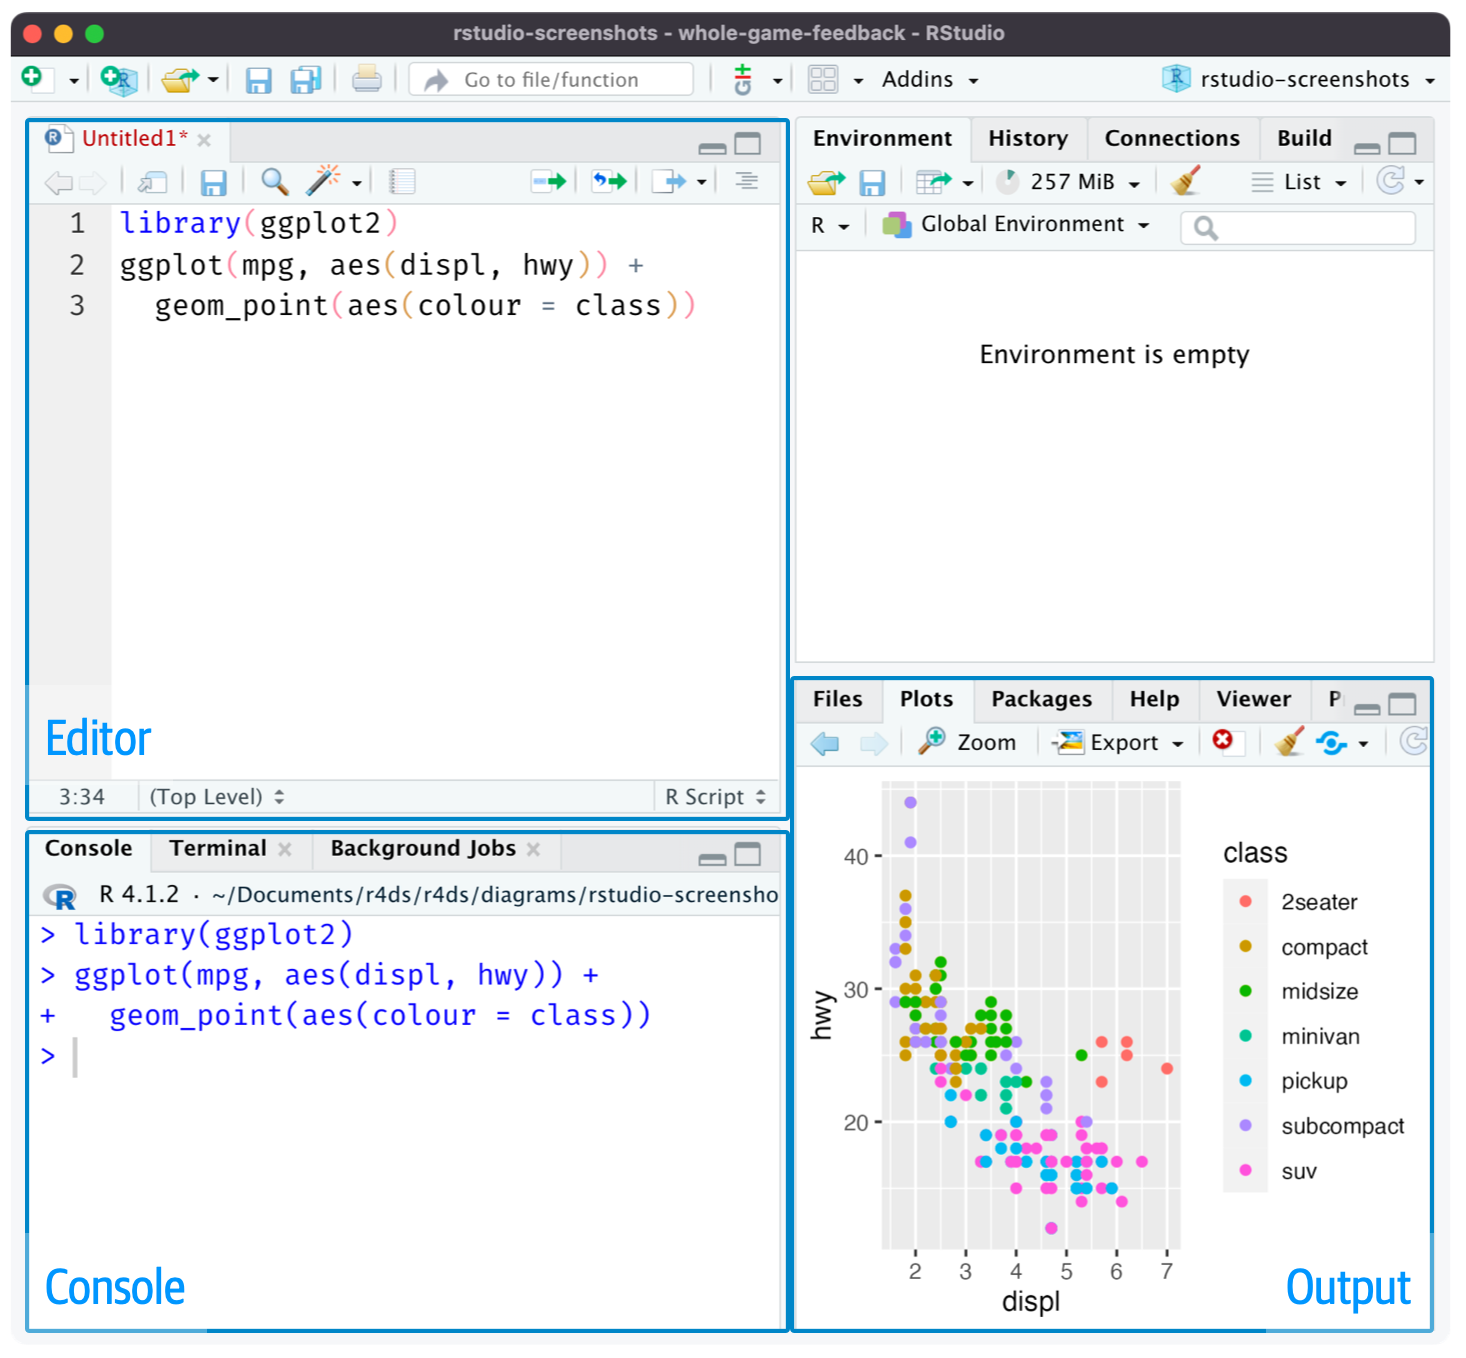
\includegraphics[keepaspectratio]{chapters/images/rstudio_interface.png}}

}

\end{figure}%

\subsection{The Script Editor}\label{the-script-editor}

The Script Editor is where you write your R code in script files. A
script file is simply a text file containing R code that can be saved,
edited, and run again later. Working in script files is essential for
reproducibility---you can always go back and see exactly what you did,
make changes, and re-run your analysis. To open a new script file, go to
File → New File → R Script, or use the keyboard shortcut Cmd+Shift+N
(Mac) or Ctrl+Shift+N (Windows/Linux).

\subsection{The Console}\label{the-console}

The Console is where R actually executes your code. When you run code
from a script, it gets sent to the console line by line. You can also
type code directly into the console and press Enter to run it
immediately. However, code typed directly into the console is not saved,
so this approach is generally only recommended for quick tests or
exploratory work. Output from many functions, including regression
results, will be printed to the console.

\subsection{The Environment Panel}\label{the-environment-panel}

The Environment panel displays all the ``objects'' you have created in
your current R session. These objects might include data frames,
vectors, or stored values. You can see each object's name along with a
brief summary of its contents. This panel is useful for keeping track of
what data and variables you currently have available.

\subsection{The Plots and Output
Panel}\label{the-plots-and-output-panel}

This panel serves multiple purposes. When you create visualizations
(like scatter plots or histograms), they will appear here. This panel
also contains tabs for browsing files on your computer, viewing
installed packages, and accessing R's built-in help documentation.

\begin{tcolorbox}[enhanced jigsaw, arc=.35mm, bottomrule=.15mm, bottomtitle=1mm, breakable, colback=white, colbacktitle=quarto-callout-tip-color!10!white, colframe=quarto-callout-tip-color-frame, coltitle=black, left=2mm, leftrule=.75mm, opacityback=0, opacitybacktitle=0.6, rightrule=.15mm, title=\textcolor{quarto-callout-tip-color}{\faLightbulb}\hspace{0.5em}{Customizing Your Layout}, titlerule=0mm, toprule=.15mm, toptitle=1mm]

You can hide or show different panels under the ``View'' menu. This is
useful when you want more screen space for a particular task, such as
focusing on your script while writing code.

\end{tcolorbox}

\section{Basic Coding in R}\label{basic-coding-in-r}

Now that RStudio is set up, let's write some code! We'll start with
simple operations in the console to get familiar with R's syntax.

\subsection{Arithmetic Operations}\label{arithmetic-operations}

R can function as a sophisticated calculator. Try typing the following
expressions in the console and pressing Enter:

\begin{Shaded}
\begin{Highlighting}[]
\DecValTok{2} \SpecialCharTok{+} \DecValTok{2}
\end{Highlighting}
\end{Shaded}

\begin{verbatim}
[1] 4
\end{verbatim}

\begin{Shaded}
\begin{Highlighting}[]
\DecValTok{20} \SpecialCharTok{*} \DecValTok{5} \SpecialCharTok{/} \DecValTok{87}
\end{Highlighting}
\end{Shaded}

\begin{verbatim}
[1] 1.149425
\end{verbatim}

\begin{Shaded}
\begin{Highlighting}[]
\FunctionTok{sin}\NormalTok{(pi }\SpecialCharTok{/} \DecValTok{2}\NormalTok{)}
\end{Highlighting}
\end{Shaded}

\begin{verbatim}
[1] 1
\end{verbatim}

\begin{Shaded}
\begin{Highlighting}[]
\FunctionTok{sqrt}\NormalTok{(}\DecValTok{6}\NormalTok{)}
\end{Highlighting}
\end{Shaded}

\begin{verbatim}
[1] 2.44949
\end{verbatim}

As you can see, R can handle basic arithmetic as well as mathematical
functions like \texttt{sin()} and \texttt{sqrt()}. The \texttt{pi} you
see in the third example is a built-in constant in R representing the
mathematical constant \(\pi\).

\subsection{Objects and Assignment}\label{objects-and-assignment}

R is an ``object-oriented language,'' meaning that data, variables, and
nearly everything else is stored as an ``object.'' You create objects
using the assignment operator \texttt{\textless{}-}. The assignment
operator takes whatever is on the right side and stores it in the name
on the left side.

\begin{Shaded}
\begin{Highlighting}[]
\NormalTok{x }\OtherTok{\textless{}{-}} \DecValTok{2} \SpecialCharTok{+} \DecValTok{5}
\end{Highlighting}
\end{Shaded}

After running this code, the value \texttt{7} is now stored in an object
called \texttt{x}. Notice that R didn't print anything---it just stored
the value. To see what's stored in an object, type its name and press
Enter:

\begin{Shaded}
\begin{Highlighting}[]
\NormalTok{x}
\end{Highlighting}
\end{Shaded}

\begin{verbatim}
[1] 7
\end{verbatim}

You can use objects in subsequent calculations, just like variables in
algebra:

\begin{Shaded}
\begin{Highlighting}[]
\NormalTok{x }\SpecialCharTok{+} \DecValTok{10}
\end{Highlighting}
\end{Shaded}

\begin{verbatim}
[1] 17
\end{verbatim}

You can also update an object by reassigning it:

\begin{Shaded}
\begin{Highlighting}[]
\NormalTok{x }\OtherTok{\textless{}{-}}\NormalTok{ x }\SpecialCharTok{+} \DecValTok{50}
\NormalTok{x}
\end{Highlighting}
\end{Shaded}

\begin{verbatim}
[1] 57
\end{verbatim}

\begin{tcolorbox}[enhanced jigsaw, arc=.35mm, bottomrule=.15mm, bottomtitle=1mm, breakable, colback=white, colbacktitle=quarto-callout-tip-color!10!white, colframe=quarto-callout-tip-color-frame, coltitle=black, left=2mm, leftrule=.75mm, opacityback=0, opacitybacktitle=0.6, rightrule=.15mm, title=\textcolor{quarto-callout-tip-color}{\faLightbulb}\hspace{0.5em}{Naming Objects}, titlerule=0mm, toprule=.15mm, toptitle=1mm]

When creating object names, keep them short but descriptive. Object
names cannot contain spaces. Some good examples include:
\texttt{flight\_data}, \texttt{reg\_controls\_1}, \texttt{acs\_male}, or
\texttt{X\_mat}.

\end{tcolorbox}

\subsection{Vectors}\label{vectors}

A vector is the simplest type of object in R. Vectors contain a sequence
of values of the same type (all numbers, all text, etc.). You create
vectors using the \texttt{c()} function, which stands for ``combine'':

\begin{Shaded}
\begin{Highlighting}[]
\NormalTok{primes }\OtherTok{\textless{}{-}} \FunctionTok{c}\NormalTok{(}\DecValTok{2}\NormalTok{, }\DecValTok{3}\NormalTok{, }\DecValTok{5}\NormalTok{, }\DecValTok{7}\NormalTok{, }\DecValTok{11}\NormalTok{, }\DecValTok{13}\NormalTok{)}
\NormalTok{primes}
\end{Highlighting}
\end{Shaded}

\begin{verbatim}
[1]  2  3  5  7 11 13
\end{verbatim}

One powerful feature of R is that arithmetic operations on vectors are
applied element-by-element:

\begin{Shaded}
\begin{Highlighting}[]
\NormalTok{primes }\SpecialCharTok{*} \DecValTok{2}
\end{Highlighting}
\end{Shaded}

\begin{verbatim}
[1]  4  6 10 14 22 26
\end{verbatim}

\begin{Shaded}
\begin{Highlighting}[]
\NormalTok{primes }\SpecialCharTok{{-}} \DecValTok{1}
\end{Highlighting}
\end{Shaded}

\begin{verbatim}
[1]  1  2  4  6 10 12
\end{verbatim}

You can also perform arithmetic between two vectors of the same length:

\begin{Shaded}
\begin{Highlighting}[]
\NormalTok{odds }\OtherTok{\textless{}{-}} \FunctionTok{c}\NormalTok{(}\DecValTok{1}\NormalTok{, }\DecValTok{3}\NormalTok{, }\DecValTok{5}\NormalTok{, }\DecValTok{7}\NormalTok{, }\DecValTok{9}\NormalTok{, }\DecValTok{11}\NormalTok{)}
\NormalTok{primes }\SpecialCharTok{+}\NormalTok{ odds}
\end{Highlighting}
\end{Shaded}

\begin{verbatim}
[1]  3  6 10 14 20 24
\end{verbatim}

\subsection{Functions}\label{functions}

R has a large collection of built-in functions that perform specific
tasks. Functions are called using the syntax:
\texttt{function\_name(argument1\ =\ value1,\ argument2\ =\ value2,\ ...)}.

For example, the \texttt{seq()} function generates a sequence of
numbers:

\begin{Shaded}
\begin{Highlighting}[]
\NormalTok{bb }\OtherTok{\textless{}{-}} \FunctionTok{seq}\NormalTok{(}\AttributeTok{from =} \DecValTok{1}\NormalTok{, }\AttributeTok{to =} \DecValTok{30}\NormalTok{, }\AttributeTok{by =} \DecValTok{3}\NormalTok{)}
\NormalTok{bb}
\end{Highlighting}
\end{Shaded}

\begin{verbatim}
 [1]  1  4  7 10 13 16 19 22 25 28
\end{verbatim}

Here, \texttt{from}, \texttt{to}, and \texttt{by} are the
\emph{arguments} of the function. We set \texttt{from\ =\ 1} to start at
1, \texttt{to\ =\ 30} to end at 30, and \texttt{by\ =\ 3} to increment
by 3.

\begin{tcolorbox}[enhanced jigsaw, arc=.35mm, bottomrule=.15mm, bottomtitle=1mm, breakable, colback=white, colbacktitle=quarto-callout-tip-color!10!white, colframe=quarto-callout-tip-color-frame, coltitle=black, left=2mm, leftrule=.75mm, opacityback=0, opacitybacktitle=0.6, rightrule=.15mm, title=\textcolor{quarto-callout-tip-color}{\faLightbulb}\hspace{0.5em}{Getting Help}, titlerule=0mm, toprule=.15mm, toptitle=1mm]

To learn more about any function, type \texttt{?} followed by the
function name in the console. For example, \texttt{?seq} will open the
documentation for the \texttt{seq()} function.

\end{tcolorbox}

\section{Data Types in R}\label{data-types-in-r}

Every piece of data in R has a \textbf{type} that determines how it can
be used. Understanding data types is essential because certain
operations only work with certain types, and R will sometimes convert
between types automatically in ways that can cause unexpected results.

\subsection{Numeric Types}\label{numeric-types}

R has two main numeric types:

\textbf{Integer} (\texttt{int}): Whole numbers without decimal places.
Created by adding \texttt{L} after a number:

\begin{Shaded}
\begin{Highlighting}[]
\NormalTok{my\_integer }\OtherTok{\textless{}{-}} \DecValTok{5}\NormalTok{L}
\FunctionTok{typeof}\NormalTok{(my\_integer)}
\end{Highlighting}
\end{Shaded}

\begin{verbatim}
[1] "integer"
\end{verbatim}

\textbf{Double} (\texttt{dbl}): Numbers with decimal places (also called
``floating point''). This is the default for most numbers:

\begin{Shaded}
\begin{Highlighting}[]
\NormalTok{my\_double }\OtherTok{\textless{}{-}} \FloatTok{5.7}
\FunctionTok{typeof}\NormalTok{(my\_double)}
\end{Highlighting}
\end{Shaded}

\begin{verbatim}
[1] "double"
\end{verbatim}

In practice, the distinction between integers and doubles rarely matters
for econometric analysis---R handles conversions automatically. When you
see \texttt{\textless{}int\textgreater{}} or
\texttt{\textless{}dbl\textgreater{}} in your data, both are simply
``numbers.''

\subsection{Character Strings}\label{character-strings}

\textbf{Character} (\texttt{chr}): Text data, always enclosed in quotes:

\begin{Shaded}
\begin{Highlighting}[]
\NormalTok{my\_name }\OtherTok{\textless{}{-}} \StringTok{"Economics"}
\FunctionTok{typeof}\NormalTok{(my\_name)}
\end{Highlighting}
\end{Shaded}

\begin{verbatim}
[1] "character"
\end{verbatim}

Character strings are used for labels, names, and categorical data that
hasn't been converted to a factor.

\subsection{Logical Values}\label{logical-values}

\textbf{Logical} (\texttt{lgl}): TRUE or FALSE values (can be
abbreviated as \texttt{T} and \texttt{F}):

\begin{Shaded}
\begin{Highlighting}[]
\NormalTok{is\_enrolled }\OtherTok{\textless{}{-}} \ConstantTok{TRUE}
\FunctionTok{typeof}\NormalTok{(is\_enrolled)}
\end{Highlighting}
\end{Shaded}

\begin{verbatim}
[1] "logical"
\end{verbatim}

Logical values are often created by comparisons:

\begin{Shaded}
\begin{Highlighting}[]
\DecValTok{5} \SpecialCharTok{\textgreater{}} \DecValTok{3}
\end{Highlighting}
\end{Shaded}

\begin{verbatim}
[1] TRUE
\end{verbatim}

\begin{Shaded}
\begin{Highlighting}[]
\DecValTok{10} \SpecialCharTok{==} \DecValTok{10}  \CommentTok{\# Note: == tests equality, = is for assignment}
\end{Highlighting}
\end{Shaded}

\begin{verbatim}
[1] TRUE
\end{verbatim}

Logical values are essential for filtering data (e.g., ``keep only
observations where income \textgreater{} 50000'').

\subsection{Factors}\label{factors}

\textbf{Factor} (\texttt{fct}): Categorical variables with a fixed set
of possible values (called ``levels''). Factors are crucial in
regression because R treats them differently from numeric variables:

\begin{Shaded}
\begin{Highlighting}[]
\CommentTok{\# Create a factor for education level}
\NormalTok{edu\_level }\OtherTok{\textless{}{-}} \FunctionTok{factor}\NormalTok{(}\FunctionTok{c}\NormalTok{(}\StringTok{"High School"}\NormalTok{, }\StringTok{"College"}\NormalTok{, }\StringTok{"Graduate"}\NormalTok{, }\StringTok{"College"}\NormalTok{, }\StringTok{"High School"}\NormalTok{))}
\NormalTok{edu\_level}
\end{Highlighting}
\end{Shaded}

\begin{verbatim}
[1] High School College     Graduate    College     High School
Levels: College Graduate High School
\end{verbatim}

Notice how R shows the ``Levels''---the complete set of possible
categories. Factors are especially important for dummy variables in
regression.

\begin{tcolorbox}[enhanced jigsaw, arc=.35mm, bottomrule=.15mm, bottomtitle=1mm, breakable, colback=white, colbacktitle=quarto-callout-important-color!10!white, colframe=quarto-callout-important-color-frame, coltitle=black, left=2mm, leftrule=.75mm, opacityback=0, opacitybacktitle=0.6, rightrule=.15mm, title=\textcolor{quarto-callout-important-color}{\faExclamation}\hspace{0.5em}{Why Factors Matter}, titlerule=0mm, toprule=.15mm, toptitle=1mm]

When you include a factor in a regression, R automatically creates dummy
variables for each level. If you include a character variable, R may
treat it as text rather than a categorical variable, leading to errors
or unexpected results. We will talk more about this in section
Chapter~\ref{sec-dummy-nonlinear}.

\end{tcolorbox}

\subsection{Checking and Converting
Types}\label{checking-and-converting-types}

You can check an object's type with \texttt{typeof()} or
\texttt{class()}:

\begin{Shaded}
\begin{Highlighting}[]
\FunctionTok{class}\NormalTok{(edu\_level)}
\end{Highlighting}
\end{Shaded}

\begin{verbatim}
[1] "factor"
\end{verbatim}

Convert between types using \texttt{as.numeric()},
\texttt{as.character()}, \texttt{as.factor()}, etc.:

\begin{Shaded}
\begin{Highlighting}[]
\CommentTok{\# Convert character to factor}
\NormalTok{major }\OtherTok{\textless{}{-}} \FunctionTok{c}\NormalTok{(}\StringTok{"Economics"}\NormalTok{, }\StringTok{"Math"}\NormalTok{, }\StringTok{"Economics"}\NormalTok{, }\StringTok{"Physics"}\NormalTok{)}
\NormalTok{major\_factor }\OtherTok{\textless{}{-}} \FunctionTok{as.factor}\NormalTok{(major)}
\NormalTok{major\_factor}
\end{Highlighting}
\end{Shaded}

\begin{verbatim}
[1] Economics Math      Economics Physics  
Levels: Economics Math Physics
\end{verbatim}

\begin{Shaded}
\begin{Highlighting}[]
\CommentTok{\# Convert numeric to character}
\NormalTok{numbers }\OtherTok{\textless{}{-}} \FunctionTok{c}\NormalTok{(}\DecValTok{1}\NormalTok{, }\DecValTok{2}\NormalTok{, }\DecValTok{3}\NormalTok{)}
\FunctionTok{as.character}\NormalTok{(numbers)}
\end{Highlighting}
\end{Shaded}

\begin{verbatim}
[1] "1" "2" "3"
\end{verbatim}

\subsection{Common Type Abbreviations}\label{common-type-abbreviations}

When working with data frames, you'll frequently see these
abbreviations:

\begin{longtable}[]{@{}
  >{\raggedright\arraybackslash}p{(\linewidth - 6\tabcolsep) * \real{0.3333}}
  >{\raggedright\arraybackslash}p{(\linewidth - 6\tabcolsep) * \real{0.1429}}
  >{\raggedright\arraybackslash}p{(\linewidth - 6\tabcolsep) * \real{0.3095}}
  >{\raggedright\arraybackslash}p{(\linewidth - 6\tabcolsep) * \real{0.2143}}@{}}
\caption{Common data type abbreviations in
R}\label{tbl-type-abbrev}\tabularnewline
\toprule\noalign{}
\begin{minipage}[b]{\linewidth}\raggedright
Abbreviation
\end{minipage} & \begin{minipage}[b]{\linewidth}\raggedright
Type
\end{minipage} & \begin{minipage}[b]{\linewidth}\raggedright
Description
\end{minipage} & \begin{minipage}[b]{\linewidth}\raggedright
Example
\end{minipage} \\
\midrule\noalign{}
\endfirsthead
\toprule\noalign{}
\begin{minipage}[b]{\linewidth}\raggedright
Abbreviation
\end{minipage} & \begin{minipage}[b]{\linewidth}\raggedright
Type
\end{minipage} & \begin{minipage}[b]{\linewidth}\raggedright
Description
\end{minipage} & \begin{minipage}[b]{\linewidth}\raggedright
Example
\end{minipage} \\
\midrule\noalign{}
\endhead
\bottomrule\noalign{}
\endlastfoot
\texttt{\textless{}dbl\textgreater{}} & Double & Numbers with decimals &
\texttt{3.14}, \texttt{2.5} \\
\texttt{\textless{}int\textgreater{}} & Integer & Whole numbers &
\texttt{1}, \texttt{42} \\
\texttt{\textless{}chr\textgreater{}} & Character & Text strings &
\texttt{"hello"}, \texttt{"NY"} \\
\texttt{\textless{}fct\textgreater{}} & Factor & Categorical variable &
\texttt{factor("low",\ "med",\ "high")} \\
\texttt{\textless{}lgl\textgreater{}} & Logical & TRUE/FALSE &
\texttt{TRUE}, \texttt{FALSE} \\
\texttt{\textless{}date\textgreater{}} & Date & Calendar dates &
\texttt{as.Date("2024-01-15")} \\
\end{longtable}

\subsection{Data Frames}\label{data-frames}

Data frames are the primary way that structured, tabular data is stored
in R. A data frame is essentially a table where each column is a vector
and each row is an observation. R comes with several built-in data
frames for practice, including \texttt{mtcars}, which contains data on
various car models.

Use \texttt{head()} to view the first few rows of a data frame:

\begin{Shaded}
\begin{Highlighting}[]
\FunctionTok{head}\NormalTok{(mtcars)}
\end{Highlighting}
\end{Shaded}

\begin{verbatim}
                   mpg cyl disp  hp drat    wt  qsec vs am gear carb
Mazda RX4         21.0   6  160 110 3.90 2.620 16.46  0  1    4    4
Mazda RX4 Wag     21.0   6  160 110 3.90 2.875 17.02  0  1    4    4
Datsun 710        22.8   4  108  93 3.85 2.320 18.61  1  1    4    1
Hornet 4 Drive    21.4   6  258 110 3.08 3.215 19.44  1  0    3    1
Hornet Sportabout 18.7   8  360 175 3.15 3.440 17.02  0  0    3    2
Valiant           18.1   6  225 105 2.76 3.460 20.22  1  0    3    1
\end{verbatim}

You can explore the structure of a data frame using several helpful
functions:

\begin{Shaded}
\begin{Highlighting}[]
\FunctionTok{nrow}\NormalTok{(mtcars)}
\end{Highlighting}
\end{Shaded}

\begin{verbatim}
[1] 32
\end{verbatim}

\begin{Shaded}
\begin{Highlighting}[]
\FunctionTok{ncol}\NormalTok{(mtcars)}
\end{Highlighting}
\end{Shaded}

\begin{verbatim}
[1] 11
\end{verbatim}

\begin{Shaded}
\begin{Highlighting}[]
\FunctionTok{colnames}\NormalTok{(mtcars)}
\end{Highlighting}
\end{Shaded}

\begin{verbatim}
 [1] "mpg"  "cyl"  "disp" "hp"   "drat" "wt"   "qsec" "vs"   "am"   "gear"
[11] "carb"
\end{verbatim}

To access a specific column (variable) within a data frame, use the
\texttt{\$} operator:

\begin{Shaded}
\begin{Highlighting}[]
\FunctionTok{head}\NormalTok{(mtcars}\SpecialCharTok{$}\NormalTok{mpg)}
\end{Highlighting}
\end{Shaded}

\begin{verbatim}
[1] 21.0 21.0 22.8 21.4 18.7 18.1
\end{verbatim}

Here, \texttt{mtcars\$mpg} extracts the \texttt{mpg} column from the
\texttt{mtcars} data frame as a vector. I wrapped it in \texttt{head()}
to show only the first few values.

\subsection{Comments}\label{comments}

In R, anything preceded by the \texttt{\#} symbol is treated as a
comment and will not be executed. Comments are essential for documenting
your code---explaining what each section does, leaving notes for
yourself, or marking areas that need revision.

\begin{Shaded}
\begin{Highlighting}[]
\CommentTok{\# Find the mean miles per gallon}
\FunctionTok{mean}\NormalTok{(mtcars}\SpecialCharTok{$}\NormalTok{mpg)}
\end{Highlighting}
\end{Shaded}

\begin{verbatim}
[1] 20.09062
\end{verbatim}

Good commenting habits make your code readable to others (and to your
future self).

\section{Working with R Scripts}\label{working-with-r-scripts}

While the console is useful for quick tests, you should do the vast
majority of your work in script files. Scripts allow you to save your
code, edit it easily, and reproduce your entire analysis by running the
script from top to bottom.

\subsection{Creating and Running
Scripts}\label{creating-and-running-scripts}

To create a new script, go to File → New File → R Script (or use
Cmd/Ctrl + Shift + N). Write your code in the script editor, then use
the following keyboard shortcuts to run it:

\textbf{Cmd/Ctrl + Enter} executes the current line (or highlighted
selection) in the console. The cursor then automatically moves to the
next line, making it easy to step through your code line by line.

\begin{figure}

\caption{\label{fig-cursor-script}Example R script with cursor position
shown. Pressing Cmd/Ctrl + Enter will run the complete command that
creates the \texttt{not\_cancelled} object, then move the cursor to the
next statement.}

\centering{

\pandocbounded{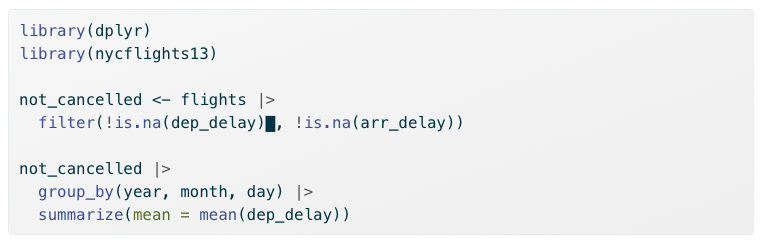
\includegraphics[keepaspectratio]{chapters/images/cursor_script.png}}

}

\end{figure}%

\textbf{Cmd/Ctrl + Shift + S} runs the entire script from top to bottom.
This is useful for checking that your complete analysis works correctly
and produces reproducible results.

\subsection{Script Best Practices}\label{script-best-practices}

Following good practices when writing scripts will save you time and
frustration. Always start your script with your name and a brief
description of the script's purpose in comments. Load all required
packages at the beginning of the script using \texttt{library()} so
anyone reading your code knows what dependencies are needed. Never
include \texttt{install.packages()} in your script---you only need to
install packages once on your computer, and you don't want your script
to install packages on someone else's machine without their permission.
Save your scripts with short, descriptive names that contain no spaces,
such as \texttt{assignment\_3.R} or \texttt{ec\_325\_data\_plotting.R}.

\section{Working Directories}\label{working-directories}

R uses a concept called the ``working directory''---the folder on your
computer where R looks for files you want to load and where it saves
files you create. You can see your current working directory at the top
of the console, or by running:

\begin{Shaded}
\begin{Highlighting}[]
\FunctionTok{getwd}\NormalTok{()}
\end{Highlighting}
\end{Shaded}

A good workflow is to save your R script in a dedicated folder for this
course (or a subfolder for each week's work), put all related data files
in the same folder, and then set your working directory to that
location. In RStudio, go to Session → Set Working Directory → To Source
File Location to automatically set the working directory to wherever
your script is saved.

\section{R Packages}\label{r-packages}

R comes with a set of ``base'' packages that provide fundamental
functionality. However, the true power of R lies in its vast ecosystem
of user-contributed packages. These packages extend R's capabilities for
specialized tasks---from data visualization to complex statistical
modeling.

\subsection{Installing Packages}\label{installing-packages}

You only need to install a package once on your computer. Use the
\texttt{install.packages()} function:

\begin{Shaded}
\begin{Highlighting}[]
\FunctionTok{install.packages}\NormalTok{(}\StringTok{"tidyverse"}\NormalTok{)}
\end{Highlighting}
\end{Shaded}

\subsection{The Tidyverse}\label{the-tidyverse}

The tidyverse is a collection of R packages designed for data science.
These packages share a common philosophy and work seamlessly together,
making data manipulation and visualization more intuitive. Some of the
most commonly used tidyverse packages include \texttt{dplyr} (data
manipulation), \texttt{ggplot2} (visualization), and \texttt{readr}
(reading data files).

Installing \texttt{tidyverse} installs all of these packages at once.

\subsection{Loading Packages}\label{loading-packages}

Once a package is installed, you need to load it each time you start a
new R session using \texttt{library()}:

\begin{Shaded}
\begin{Highlighting}[]
\FunctionTok{library}\NormalTok{(tidyverse)}
\end{Highlighting}
\end{Shaded}

When you load the \texttt{tidyverse}, you'll see a message listing which
packages were attached. You may also see messages about
``conflicts''---this just means some \texttt{tidyverse} functions have
the same name as functions in base R, and the \texttt{tidyverse}
versions will take precedence. This is normal and expected behavior.

\subsection{The Pipe Operator}\label{the-pipe-operator}

One of the most useful features of the \texttt{tidyverse} is the
\textbf{pipe operator}: \texttt{\textbar{}\textgreater{}}. The pipe
takes the result of whatever is on its left and passes it as the first
argument to the function on its right.

Think of the pipe like a conjunction in a sentence. Just as ``and'' or
``then'' connect actions in English, the pipe connects operations in R.
Instead of saying ``Take the data, then filter it, then summarize it,''
you write code that reads almost the same way:

\begin{Shaded}
\begin{Highlighting}[]
\NormalTok{data }\SpecialCharTok{|\textgreater{}}
  \FunctionTok{filter}\NormalTok{(year }\SpecialCharTok{==} \DecValTok{2020}\NormalTok{) }\SpecialCharTok{|\textgreater{}}
  \FunctionTok{summarize}\NormalTok{(}\AttributeTok{mean\_income =} \FunctionTok{mean}\NormalTok{(income))}
\end{Highlighting}
\end{Shaded}

This code reads naturally from top to bottom: ``Start with
\texttt{data}, \emph{then} filter to rows where year equals 2020,
\emph{then} summarize by calculating the mean income.''

Without the pipe, you would need to either nest functions inside each
other (hard to read) or create intermediate objects at each step
(clutters your environment). The pipe lets you write code that mirrors
how you think about the analysis.

\begin{tcolorbox}[enhanced jigsaw, arc=.35mm, bottomrule=.15mm, bottomtitle=1mm, breakable, colback=white, colbacktitle=quarto-callout-note-color!10!white, colframe=quarto-callout-note-color-frame, coltitle=black, left=2mm, leftrule=.75mm, opacityback=0, opacitybacktitle=0.6, rightrule=.15mm, title=\textcolor{quarto-callout-note-color}{\faInfo}\hspace{0.5em}{Base R Pipe vs.~Magrittr Pipe}, titlerule=0mm, toprule=.15mm, toptitle=1mm]

R now has a built-in pipe (\texttt{\textbar{}\textgreater{}}) that works
without loading any packages. The \texttt{tidyverse} historically used
\texttt{\%\textgreater{}\%} from the \texttt{magrittr} package, which
you may see other people use. Both work similarly for most purposes.
We'll use the base R pipe \texttt{\textbar{}\textgreater{}} in this
course.

\end{tcolorbox}

\begin{tcolorbox}[enhanced jigsaw, arc=.35mm, bottomrule=.15mm, bottomtitle=1mm, breakable, colback=white, colbacktitle=quarto-callout-important-color!10!white, colframe=quarto-callout-important-color-frame, coltitle=black, left=2mm, leftrule=.75mm, opacityback=0, opacitybacktitle=0.6, rightrule=.15mm, title=\textcolor{quarto-callout-important-color}{\faExclamation}\hspace{0.5em}{Remember the Difference}, titlerule=0mm, toprule=.15mm, toptitle=1mm]

\texttt{install.packages()} downloads and installs a package to your
computer (do this once). \texttt{library()} loads an already-installed
package into your current R session (do this every time you start R).

\end{tcolorbox}

\section{Summary and Conclusion}\label{summary-and-conclusion-3}

This appendix walked you through the essential first steps for working
with R. You installed R and RStudio, learned how the RStudio interface
is organized, and wrote your first R code. You now understand how to
create and manipulate objects, work with vectors and data frames, write
and run scripts, and install packages.

\subsection{Key Takeaways}\label{key-takeaways-5}

\begin{itemize}
\item
  \textbf{RStudio is your interface to R:} Always work in RStudio, not
  base R. The script editor, console, environment, and plots panels each
  serve distinct purposes in your workflow.
\item
  \textbf{Scripts are essential for reproducibility:} Write your code in
  script files that you can save, edit, and re-run. Use comments to
  document what your code does.
\item
  \textbf{Objects store everything in R:} Use the assignment operator
  \texttt{\textless{}-} to create objects. Vectors hold sequences of
  values; data frames hold structured tabular data.
\item
  \textbf{Packages extend R's capabilities:} Install packages once with
  \texttt{install.packages()}, then load them each session with
  \texttt{library()}. The tidyverse is a particularly useful collection
  of packages for data science.
\item
  \textbf{Working directories matter:} Set your working directory to the
  folder containing your script and data files to keep your analysis
  organized.
\end{itemize}

With these foundations in place, you are ready to start loading real
data, creating visualizations, and running econometric analyses.

\section{Check Your Understanding}\label{check-your-understanding-13}

\emph{Note: This section contains interactive content only available in
the HTML version.}

\chapter{Statistics and Probability Review}\label{sec-stats-review}

\begin{tcolorbox}[enhanced jigsaw, arc=.35mm, bottomrule=.15mm, bottomtitle=1mm, breakable, colback=white, colbacktitle=quarto-callout-tip-color!10!white, colframe=quarto-callout-tip-color-frame, coltitle=black, left=2mm, leftrule=.75mm, opacityback=0, opacitybacktitle=0.6, rightrule=.15mm, title=\textcolor{quarto-callout-tip-color}{\faLightbulb}\hspace{0.5em}{\textbf{Key Questions}}, titlerule=0mm, toprule=.15mm, toptitle=1mm]

\begin{itemize}
\tightlist
\item
  What are the properties of the summation operator?
\item
  What are the key rules for logarithms, and why do economists use logs
  so often?
\item
  How do we interpret derivatives and partial derivatives?
\item
  How do we find the maximum or minimum of a function?
\item
  What is the difference between a population and a sample?
\item
  What is a random variable and how do we describe its distribution?
\item
  How do we measure central tendency, variability, and relationships
  between variables?
\item
  What is the normal distribution and why is it important?
\end{itemize}

\end{tcolorbox}

\begin{tcolorbox}[enhanced jigsaw, arc=.35mm, bottomrule=.15mm, bottomtitle=1mm, breakable, colback=white, colbacktitle=quarto-callout-note-color!10!white, colframe=quarto-callout-note-color-frame, coltitle=black, left=2mm, leftrule=.75mm, opacityback=0, opacitybacktitle=0.6, rightrule=.15mm, title=\textcolor{quarto-callout-note-color}{\faInfo}\hspace{0.5em}{\textbf{Suggested Readings}}, titlerule=0mm, toprule=.15mm, toptitle=1mm]

\begin{itemize}
\tightlist
\item
  Wooldridge (2019), Appendix A, B, and C
\end{itemize}

\end{tcolorbox}

This appendix reviews the essential mathematical and statistical
concepts that form the foundation for econometrics. If you've taken
introductory statistics or calculus, much of this material will be
familiar. However, econometrics uses these tools in specific ways, so
it's worth reviewing them with an eye toward how they'll appear
throughout the course.

\section{Basic Mathematical Tools}\label{basic-mathematical-tools}

\subsection{The Summation Operator}\label{the-summation-operator}

The summation operator provides a compact way to write the sum of a
sequence of numbers. If \(\{x_i: i = 1, 2, ..., n\}\) is a sequence of
\(n\) numbers, then the sum of these numbers is written as:

\[
x_1 + x_2 + ... + x_n = \sum_{i=1}^{n} x_i
\]

The symbol \(\Sigma\) (capital Greek letter sigma) tells us to add up
the terms. The expression \(i=1\) below the sigma indicates that we
start counting at \(i=1\), and the \(n\) above tells us to stop at
\(i=n\).

\subsubsection{Properties of Summation}\label{properties-of-summation}

The summation operator has several useful properties that we will use
frequently.

\textbf{Property 1: Summing a constant.} If we add a constant \(c\) to
itself \(n\) times, we get \(n\) times the constant:

\[
\sum_{i=1}^{n} c = nc
\]

\textbf{Property 2: Factoring out constants.} We can pull constants
outside the summation:

\[
\sum_{i=1}^{n} cx_i = c \sum_{i=1}^{n} x_i
\]

\textbf{Property 3: Separating additive terms.} Sums can be split across
addition:

\[
\sum_{i=1}^{n} (ax_i + by_i) = a\sum_{i=1}^{n} x_i + b\sum_{i=1}^{n} y_i
\]

\begin{tcolorbox}[enhanced jigsaw, arc=.35mm, bottomrule=.15mm, bottomtitle=1mm, breakable, colback=white, colbacktitle=quarto-callout-warning-color!10!white, colframe=quarto-callout-warning-color-frame, coltitle=black, left=2mm, leftrule=.75mm, opacityback=0, opacitybacktitle=0.6, rightrule=.15mm, title=\textcolor{quarto-callout-warning-color}{\faExclamationTriangle}\hspace{0.5em}{Common Mistakes with Summation}, titlerule=0mm, toprule=.15mm, toptitle=1mm]

These properties do \textbf{not} extend to division or multiplication in
the ways you might expect.

We \textbf{cannot} break up divided expressions: \[
\sum_{i=1}^{n} \frac{x_i}{y_i} \neq \frac{\sum_{i=1}^{n} x_i}{\sum_{i=1}^{n} y_i}
\]

We \textbf{cannot} break up multiplicative expressions: \[
\sum_{i=1}^{n} x_i^2 \neq \left(\sum_{i=1}^{n} x_i\right)^2
\]

\end{tcolorbox}

\subsubsection{The Sample Mean}\label{the-sample-mean}

Given \(n\) numbers \(\{x_i: i = 1, 2, ..., n\}\), we can compute their
\textbf{average} or \textbf{mean} value by adding them up and dividing
by \(n\). The average value, denoted \(\bar{x}\) (read ``x-bar''), is
written as:

\[
\bar{x} = \frac{1}{n} \sum_{i=1}^{n} x_i
\]

The average is an example of a \textbf{descriptive statistic}: a value
that describes or summarizes a characteristic of a set of data points.
In this case, the mean describes the \textbf{central tendency} of
\(x_i\)---where the ``middle'' of the data lies.

\subsubsection{Useful Summation Results}\label{useful-summation-results}

Two results involving summations will appear repeatedly in this course.

\textbf{Result 1: Deviations from the mean sum to zero.} The sum of the
deviations \((x_i - \bar{x})\) from the mean always equals zero:

\[
\sum_{i=1}^{n} (x_i - \bar{x}) = 0
\]

This can be proven using the properties above:

\[
\sum_{i=1}^{n} (x_i - \bar{x}) = \sum_{i=1}^{n} x_i - \sum_{i=1}^{n} \bar{x} = \sum_{i=1}^{n} x_i - n\bar{x} = n\bar{x} - n\bar{x} = 0
\]

The last step follows because
\(\bar{x} = \frac{1}{n}\sum_{i=1}^{n} x_i\) implies
\(n\bar{x} = \sum_{i=1}^{n} x_i\).

\textbf{Result 2: Sum of squared deviations.} The sum of squared
deviations can be rewritten as:

\[
\sum_{i=1}^{n} (x_i - \bar{x})^2 = \sum_{i=1}^{n} x_i^2 - n\bar{x}^2
\]

More generally, for two variables \(x\) and \(y\):

\[
\sum_{i=1}^{n} (x_i - \bar{x})(y_i - \bar{y}) = \sum_{i=1}^{n} x_i y_i - n\bar{x}\bar{y}
\]

These identities are useful for computing variances and covariances,
which we will discuss shortly.

\subsection{Derivatives}\label{derivatives}

The derivative \(\frac{dy}{dx}\) of a function \(y = f(x)\) measures its
\textbf{instantaneous rate of change}. It tells you how sensitive the
function's output is to a small change in its input. In econometrics,
derivatives help us interpret how changes in independent variables
affect dependent variables.

Here are derivatives of some common functional forms in econometrics:

{\def\LTcaptype{none} % do not increment counter
\begin{longtable}[]{@{}
  >{\raggedright\arraybackslash}p{(\linewidth - 2\tabcolsep) * \real{0.4545}}
  >{\raggedright\arraybackslash}p{(\linewidth - 2\tabcolsep) * \real{0.5455}}@{}}
\toprule\noalign{}
\begin{minipage}[b]{\linewidth}\raggedright
Function
\end{minipage} & \begin{minipage}[b]{\linewidth}\raggedright
Derivative
\end{minipage} \\
\midrule\noalign{}
\endhead
\bottomrule\noalign{}
\endlastfoot
\(y = \beta_0 + \beta_1 x\) & \(\frac{dy}{dx} = \beta_1\) \\
\(y = \beta_0 + \beta_1 x + \beta_2 x^2\) &
\(\frac{dy}{dx} = \beta_1 + 2\beta_2 x\) \\
\(y = \beta_0 + \frac{\beta_1}{x}\) &
\(\frac{dy}{dx} = -\frac{\beta_1}{x^2}\) \\
\(y = \beta_0 + \beta_1 \ln(x)\) &
\(\frac{dy}{dx} = \frac{\beta_1}{x}\) \\
\end{longtable}
}

Notice that in the linear case, the derivative is simply the coefficient
\(\beta_1\)---the effect of \(x\) on \(y\) is constant. In the other
cases, the derivative depends on the value of \(x\), meaning the effect
of \(x\) on \(y\) varies depending on where you start.

\subsection{Percentages and Percent
Changes}\label{percentages-and-percent-changes}

Understanding percentages is essential for econometrics. Many economic
variables are reported as percentages (unemployment rate, interest
rates, inflation), and we frequently describe changes in percentage
terms. Getting the language right matters---confusing ``percent'' with
``percentage points'' is a common source of errors.

\subsubsection{Percentages}\label{percentages}

A \textbf{percentage} expresses a number as a fraction of 100. To
convert a decimal to a percentage, multiply by 100:

\[0.25 = 25\%\]

To convert a percentage to a decimal, divide by 100:

\[25\% = 0.25\]

In econometrics, we typically work with decimals in our calculations and
convert to percentages for interpretation.

\subsubsection{Percent Change}\label{percent-change}

The \textbf{percent change} (or \textbf{percentage change}) measures how
much a variable changed relative to its initial value:

\[\text{Percent Change} = \frac{\text{New Value} - \text{Old Value}}{\text{Old Value}} \times 100\%\]

Or more compactly:

\[\%\Delta Y = \frac{Y_2 - Y_1}{Y_1} \times 100\%\]

\textbf{Example:} If wages increase from \$20 to \$22 per hour:

\[\%\Delta wage = \frac{22 - 20}{20} \times 100\% = \frac{2}{20} \times 100\% = 10\%\]

Wages increased by \textbf{10 percent}.

\begin{tcolorbox}[enhanced jigsaw, arc=.35mm, bottomrule=.15mm, bottomtitle=1mm, breakable, colback=white, colbacktitle=quarto-callout-warning-color!10!white, colframe=quarto-callout-warning-color-frame, coltitle=black, left=2mm, leftrule=.75mm, opacityback=0, opacitybacktitle=0.6, rightrule=.15mm, title=\textcolor{quarto-callout-warning-color}{\faExclamationTriangle}\hspace{0.5em}{Percent Change vs.~Percentage Point Change}, titlerule=0mm, toprule=.15mm, toptitle=1mm]

These are \textbf{not} the same thing! This distinction trips up many
students.

\begin{itemize}
\tightlist
\item
  \textbf{Percent change:} The change relative to the starting value
\item
  \textbf{Percentage point change:} The arithmetic difference between
  two percentages
\end{itemize}

\textbf{Example:} If the unemployment rate rises from 4\% to 5\%:

\begin{itemize}
\tightlist
\item
  The \textbf{percentage point change} is: \(5\% - 4\% = 1\) percentage
  point
\item
  The \textbf{percent change} is:
  \(\frac{5 - 4}{4} \times 100\% = 25\%\)
\end{itemize}

Both statements are correct:

\begin{itemize}
\tightlist
\item
  ``Unemployment rose by 1 percentage point''
\item
  ``Unemployment rose by 25 percent''
\end{itemize}

They mean very different things! In news and policy discussions, this
distinction matters enormously.

\end{tcolorbox}

\subsubsection{When to Use Which}\label{when-to-use-which}

Use \textbf{percentage points} when:

\begin{itemize}
\tightlist
\item
  Describing changes in variables already measured as percentages
  (interest rates, unemployment rates, test scores out of 100)
\item
  You want to describe the absolute change in the percentage
\end{itemize}

Use \textbf{percent change} when:

\begin{itemize}
\tightlist
\item
  Describing changes in levels (wages, prices, GDP, population)
\item
  You want to describe the relative or proportional change
\end{itemize}

\textbf{Example:} An interest rate cut from 5\% to 4\% is:

\begin{itemize}
\tightlist
\item
  A 1 percentage point decrease ✓
\item
  A 20\% decrease ✓ (both are correct, but mean different things)
\item
  \st{A 1\% decrease} ✗ (this is ambiguous and often wrong)
\end{itemize}

\subsubsection{Calculating Values After Percent
Changes}\label{calculating-values-after-percent-changes}

If \(Y\) increases by \(p\%\), the new value is:

\[Y_{new} = Y_{old} \times (1 + p/100)\]

If \(Y\) decreases by \(p\%\), the new value is:

\[Y_{new} = Y_{old} \times (1 - p/100)\]

\textbf{Example:} If a \$50 item increases in price by 20\%:

\[Price_{new} = 50 \times (1 + 0.20) = 50 \times 1.20 = \$60\]

\subsubsection{Compounding Percent
Changes}\label{compounding-percent-changes}

Percent changes don't add---they compound. If wages increase by 10\% and
then by another 10\%, the total increase is \textbf{not} 20\%.

\[\text{Final} = \text{Initial} \times 1.10 \times 1.10 = \text{Initial} \times 1.21\]

The total increase is \textbf{21\%}, not 20\%.

This is why we use logarithms: log changes \textbf{do} add up, making
them convenient for analyzing growth over time.

\subsection{Logarithms}\label{logarithms}

Logarithms appear constantly in econometrics. We use them to model
percentage changes, interpret coefficients as elasticities, and
transform skewed variables like income and wages. Understanding log
rules is essential for working with regression models.

\subsubsection{What is a Logarithm?}\label{what-is-a-logarithm}

The natural logarithm, denoted \(\ln(x)\), is the inverse of the
exponential function \(e^x\). If \(y = \ln(x)\), then \(e^y = x\).

Some key values to remember:

\begin{itemize}
\tightlist
\item
  \(\ln(1) = 0\) because \(e^0 = 1\)
\item
  \(\ln(e) = 1\) because \(e^1 = e\)
\item
  \(\ln(x)\) is only defined for \(x > 0\)
\end{itemize}

\subsubsection{Essential Log Rules}\label{essential-log-rules}

Three rules form the foundation for working with logarithms:

\textbf{Rule 1: Product Rule.} The log of a product is the sum of the
logs: \[\ln(ab) = \ln(a) + \ln(b)\]

\textbf{Rule 2: Quotient Rule.} The log of a ratio is the difference of
the logs: \[\ln\left(\frac{a}{b}\right) = \ln(a) - \ln(b)\]

\textbf{Rule 3: Power Rule.} The log of a power brings the exponent
down: \[\ln(a^k) = k \ln(a)\]

These rules are used constantly when manipulating regression equations
and interpreting coefficients.

\subsubsection{Logs and Percentage
Changes}\label{logs-and-percentage-changes}

Here is the most important property of logs for econometrics:

\begin{tcolorbox}[enhanced jigsaw, arc=.35mm, bottomrule=.15mm, bottomtitle=1mm, breakable, colback=white, colbacktitle=quarto-callout-important-color!10!white, colframe=quarto-callout-important-color-frame, coltitle=black, left=2mm, leftrule=.75mm, opacityback=0, opacitybacktitle=0.6, rightrule=.15mm, title=\textcolor{quarto-callout-important-color}{\faExclamation}\hspace{0.5em}{The Key Insight}, titlerule=0mm, toprule=.15mm, toptitle=1mm]

For small changes, the \textbf{difference in logs approximately equals
the percentage change}:
\[\ln(Y_2) - \ln(Y_1) \approx \frac{Y_2 - Y_1}{Y_1}\]

In other words: \textbf{\(\Delta ln(Y) \approx \%\) change in Y}

\end{tcolorbox}

This approximation works well for changes up to about 20\%. It follows
from the quotient rule:
\[\ln(Y_2) - \ln(Y_1) = \ln\left(\frac{Y_2}{Y_1}\right)\]

When \(Y_2\) is close to \(Y_1\), the ratio \(Y_2/Y_1\) is close to 1,
and \(\ln(1 + x) \approx x\) for small \(x\).

\textbf{Example:} If \(\ln(wage)\) increases from 2.50 to 2.58, the
change is \(0.08\). This means wages increased by approximately
\textbf{8\%}.

\subsubsection{Other Uses of Logs}\label{other-uses-of-logs}

Logarithms are useful in economics for several reasons:

\begin{enumerate}
\def\labelenumi{\arabic{enumi}.}
\item
  \textbf{Percentage interpretation:} Coefficients in log models have
  natural percentage interpretations (more on this in
  Chapter~\ref{sec-dummy-nonlinear}).
\item
  \textbf{Elasticities:} In a log-log model like
  \(\ln(Y) = \beta_0 + \beta_1 \ln(X)\), the coefficient \(\beta_1\) is
  the \textbf{elasticity}---the percentage change in \(Y\) for a 1\%
  change in \(X\).
\item
  \textbf{Reducing skewness:} Variables like income, wages, and prices
  are often right-skewed. Taking logs makes them more symmetric and
  closer to normal.
\item
  \textbf{Multiplicative relationships:} Logs transform multiplicative
  relationships into additive ones, which are easier to estimate with
  linear regression.
\end{enumerate}

\begin{figure}

\caption{\label{fig-log-transform}Left: The distribution of wages is
right-skewed. Right: The distribution of log wages is more symmetric.}

\centering{


\includegraphics[width=0.85\linewidth,height=\textheight,keepaspectratio]{chapters/statsreview_files/figure-pdf/fig-log-transform-1.pdf}

}

\end{figure}%

\subsection{Partial Derivatives}\label{partial-derivatives}

When \(y\) is a function of multiple variables, say \(y = f(x_1, x_2)\),
we use \textbf{partial derivatives} to measure how \(y\) changes with
respect to one variable while holding the others constant.

The partial derivative of \(y\) with respect to \(x_1\), holding \(x_2\)
constant, is denoted \(\frac{\partial y}{\partial x_1}\). Similarly, the
partial derivative with respect to \(x_2\), holding \(x_1\) constant, is
\(\frac{\partial y}{\partial x_2}\).

For example, if \(y = \beta_0 + \beta_1 x_1 + \beta_2 x_2\), then:

\[
\frac{\partial y}{\partial x_1} = \beta_1, \qquad \frac{\partial y}{\partial x_2} = \beta_2
\]

The concept of ``holding other variables constant'' is central to
econometrics. When we estimate a regression coefficient, we are trying
to measure the partial effect of one variable on the outcome,
controlling for other factors.

\subsection{Optimization: Maxima and
Minima}\label{optimization-maxima-and-minima}

In econometrics, we often need to find the value of a variable that
maximizes or minimizes a function. For example, Ordinary Least Squares
(OLS) regression finds coefficient estimates by minimizing the sum of
squared residuals. Understanding optimization is essential for
understanding how these estimates are derived.

\subsubsection{Finding Critical Points}\label{finding-critical-points}

To find the maximum or minimum of a function \(f(x)\), we take the
derivative, set it equal to zero, and solve for \(x\). The solutions are
called \textbf{critical points}.

For example, consider the quadratic function:

\[
f(x) = ax^2 + bx + c
\]

Taking the derivative and setting it equal to zero:

\[
\frac{df}{dx} = 2ax + b = 0
\]

Solving for \(x\):

\[
x^* = -\frac{b}{2a}
\]

This critical point \(x^*\) is where the function reaches its maximum or
minimum.

\subsubsection{Determining Maximum
vs.~Minimum}\label{determining-maximum-vs.-minimum}

How do we know if a critical point is a maximum or a minimum? We use the
\textbf{second derivative test}. The second derivative tells us about
the curvature of the function:

\[
\frac{d^2f}{dx^2} = 2a
\]

The rule is:

\begin{itemize}
\tightlist
\item
  If \(\frac{d^2f}{dx^2} > 0\) at the critical point, the function is
  \textbf{concave up} (bowl-shaped), and we have a \textbf{minimum}
\item
  If \(\frac{d^2f}{dx^2} < 0\) at the critical point, the function is
  \textbf{concave down} (hill-shaped), and we have a \textbf{maximum}
\end{itemize}

For our quadratic function \(f(x) = ax^2 + bx + c\):

\begin{itemize}
\tightlist
\item
  If \(a > 0\): The parabola opens upward, and \(x^* = -\frac{b}{2a}\)
  is a \textbf{minimum}
\item
  If \(a < 0\): The parabola opens downward, and \(x^* = -\frac{b}{2a}\)
  is a \textbf{maximum}
\end{itemize}

\begin{figure}

\caption{\label{fig-quadratic-optimization}Left: When a \textgreater{}
0, the parabola opens upward and the critical point is a minimum. Right:
When a \textless{} 0, the parabola opens downward and the critical point
is a maximum.}

\centering{


\includegraphics[width=0.85\linewidth,height=\textheight,keepaspectratio]{chapters/statsreview_files/figure-pdf/fig-quadratic-optimization-1.pdf}

}

\end{figure}%

\begin{tcolorbox}[enhanced jigsaw, arc=.35mm, bottomrule=.15mm, bottomtitle=1mm, breakable, colback=white, colbacktitle=quarto-callout-tip-color!10!white, colframe=quarto-callout-tip-color-frame, coltitle=black, left=2mm, leftrule=.75mm, opacityback=0, opacitybacktitle=0.6, rightrule=.15mm, title=\textcolor{quarto-callout-tip-color}{\faLightbulb}\hspace{0.5em}{Optimization in OLS}, titlerule=0mm, toprule=.15mm, toptitle=1mm]

In OLS regression, we minimize the sum of squared residuals, which is a
quadratic function of the coefficients. The second derivative is
positive (the function is convex), confirming that the solution is
indeed a minimum. This is why setting the first derivative equal to zero
gives us the best-fitting line.

\end{tcolorbox}

\subsubsection{Optimization with Multiple
Variables}\label{optimization-with-multiple-variables}

When a function depends on multiple variables, we find critical points
by setting all partial derivatives equal to zero simultaneously. For a
function \(f(x_1, x_2)\):

\[
\frac{\partial f}{\partial x_1} = 0 \quad \text{and} \quad \frac{\partial f}{\partial x_2} = 0
\]

Determining whether a critical point is a maximum, minimum, or neither
(a saddle point) requires examining the second partial derivatives,
which we will encounter when deriving the OLS estimator.

\section{Population vs.~Sample}\label{population-vs.-sample}

Before diving into probability, it's important to understand the
distinction between a \textbf{population} and a \textbf{sample}, as this
distinction underlies all of statistical inference.

The \textbf{population} is the entire group of individuals, objects, or
observations that we are interested in studying. For example, if we want
to understand the wages of all U.S. workers, the population is every
person employed in the United States. If we want to know the effect of a
drug on blood pressure, the population might be all adults with
hypertension.

In practice, we almost never observe the entire population. Instead, we
collect data on a \textbf{sample}---a subset of the population. We might
survey 5,000 workers rather than all 160 million, or run a clinical
trial with 500 patients rather than everyone with hypertension.

\begin{tcolorbox}[enhanced jigsaw, arc=.35mm, bottomrule=.15mm, bottomtitle=1mm, breakable, colback=white, colbacktitle=quarto-callout-important-color!10!white, colframe=quarto-callout-important-color-frame, coltitle=black, left=2mm, leftrule=.75mm, opacityback=0, opacitybacktitle=0.6, rightrule=.15mm, title=\textcolor{quarto-callout-important-color}{\faExclamation}\hspace{0.5em}{The Goal of Statistical Inference}, titlerule=0mm, toprule=.15mm, toptitle=1mm]

The fundamental goal of statistics is to use information from a
\textbf{sample} to draw conclusions about the \textbf{population}. We
observe sample statistics (like the sample mean \(\bar{x}\)) and use
them to make inferences about population parameters (like the population
mean \(\mu\)).

\end{tcolorbox}

This distinction affects our notation:

{\def\LTcaptype{none} % do not increment counter
\begin{longtable}[]{@{}lll@{}}
\toprule\noalign{}
Concept & Population Parameter & Sample Statistic \\
\midrule\noalign{}
\endhead
\bottomrule\noalign{}
\endlastfoot
Mean & \(\mu\) & \(\bar{x}\) \\
Variance & \(\sigma^2\) & \(s^2\) \\
Standard deviation & \(\sigma\) & \(s\) \\
Correlation & \(\rho\) & \(r\) \\
\end{longtable}
}

Population parameters are typically denoted with Greek letters and are
usually unknown. Sample statistics are computed from our data and are
used to estimate the population parameters.

For example, if we want to know the average wage of all U.S. workers
(\(\mu\)), we collect a sample and compute the sample mean
(\(\bar{x}\)). Under certain conditions, \(\bar{x}\) is a good estimate
of \(\mu\). Much of econometrics is about understanding when and how
well sample statistics estimate population parameters, and quantifying
the uncertainty in those estimates.

\section{Probability Basics}\label{probability-basics}

\subsection{Random Variables}\label{random-variables}

A \textbf{random variable} is a variable whose value is determined by a
random phenomenon. It represents a number, but the exact value is
determined by chance. Examples include the outcome of a dice roll,
whether a coin lands heads or tails, or the percentage of flights that
arrive on time.

Most variables we work with in econometrics can be thought of as random
variables. A person's wage, years of education, or health status all
have elements of randomness---we cannot perfectly predict them in
advance.

\subsection{Probability}\label{probability}

\textbf{Probability} quantifies uncertainty. If \(X\) is a random
variable that takes on \(k\) possible values \(\{x_1, x_2, ..., x_k\}\),
then the probability that \(X\) takes a particular value \(x_j\) is
denoted:

\[
p_j = P(X = x_j)
\]

Each probability \(p_j\) must be between 0 and 1, and the probabilities
must sum to 1: \(p_1 + p_2 + ... + p_k = 1\).

\subsection{Probability Distributions}\label{probability-distributions}

The \textbf{probability density function (pdf)}, denoted \(f(x)\), gives
the probability that a random variable takes on a particular value
\(x\). For discrete random variables, \(f(x) = P(X = x)\).

The \textbf{cumulative distribution function (cdf)}, denoted \(F(x)\),
gives the probability that the random variable is less than or equal to
\(x\):

\[
F(x) = P(X \leq x)
\]

The cdf is useful for answering questions like ``what is the probability
that \(X\) is below some threshold?''

\subsection{Expected Values}\label{expected-values}

The \textbf{expected value} (or \textbf{mathematical expectation}) of a
random variable \(X\), denoted \(E[X]\), represents the ``average''
outcome we would expect if we could repeat the random process many
times. It is our population ``best guess'' for the value of \(X\). We
often denote it with \(\mu\) or \(\mu_X\).

For a discrete random variable with pdf \(f(x)\), the expected value is
the weighted average of all possible values, where the weights are the
probabilities:

\[
E[X] = \sum_{j=1}^{k} x_j f(x_j) = \mu
\]

\textbf{Example:} Let \(X\) be the outcome of rolling a fair six-sided
die. Each value (1 through 6) has probability \(1/6\). The expected
value is:

\[
E[X] = \frac{1}{6}(1) + \frac{1}{6}(2) + \frac{1}{6}(3) + \frac{1}{6}(4) + \frac{1}{6}(5) + \frac{1}{6}(6) = 3.5
\]

Notice that 3.5 is not a possible outcome of any single roll, but it is
the average we would expect over many rolls.

\subsubsection{Properties of Expected
Values}\label{properties-of-expected-values}

The properties of expected values mirror those of the summation operator
and are essential for working with regression models.

\textbf{Property 1: Expected value of a constant.} The expected value of
a constant is simply that constant: \[E[c] = c\]

This makes intuitive sense: if there is no randomness, the ``expected''
value is just the value itself.

\textbf{Property 2: Multiplication by a constant.} Constants can be
factored out of the expectation operator: \[E[cX] = cE[X]\]

If you double a random variable, its expected value doubles.

\textbf{Property 3: Additivity (Linearity).} The expectation of a sum
equals the sum of expectations: \[E[X + Y] = E[X] + E[Y]\]

Importantly, this property holds \textbf{regardless of whether \(X\) and
\(Y\) are independent}. This is one of the most useful properties in
econometrics.

\textbf{Property 4: Combining the above.} Combining Properties 1, 2, and
3, we get the general linearity property:
\[E[aX + bY + c] = aE[X] + bE[Y] + c\]

This is extremely useful for working with regression equations. If
\(Y = \beta_0 + \beta_1 X + u\), we can take expectations of both sides
and apply this property.

\textbf{Property 5: Product of independent variables.} If \(X\) and
\(Y\) are \textbf{independent} random variables, then:
\[E[XY] = E[X]E[Y]\]

\begin{tcolorbox}[enhanced jigsaw, arc=.35mm, bottomrule=.15mm, bottomtitle=1mm, breakable, colback=white, colbacktitle=quarto-callout-warning-color!10!white, colframe=quarto-callout-warning-color-frame, coltitle=black, left=2mm, leftrule=.75mm, opacityback=0, opacitybacktitle=0.6, rightrule=.15mm, title=\textcolor{quarto-callout-warning-color}{\faExclamationTriangle}\hspace{0.5em}{Independence Required!}, titlerule=0mm, toprule=.15mm, toptitle=1mm]

This property only holds when \(X\) and \(Y\) are independent. If they
are correlated, \(E[XY] \neq E[X]E[Y]\) in general. In fact,
\(E[XY] - E[X]E[Y] = \text{Cov}(X,Y)\).

\end{tcolorbox}

\textbf{Property 6: Expectation of a function (Jensen's Inequality).} In
general, the expectation of a function is \textbf{not} equal to the
function of the expectation: \[E[g(X)] \neq g(E[X])\]

For example, \(E[X^2] \neq (E[X])^2\). The difference between these two
quantities is related to the variance:
\(E[X^2] - (E[X])^2 = \text{Var}(X)\).

\section{Measures of Variability}\label{measures-of-variability}

Knowing the central tendency of a variable is useful, but it doesn't
tell us everything. Two distributions can have the same mean but look
very different if one is tightly clustered around the mean while the
other is spread out. We need measures of \textbf{variability} or
\textbf{dispersion}.

\subsection{Variance}\label{variance}

Let \(X\) be a random variable with mean \(\mu = E[X]\). The
\textbf{variance} of \(X\), denoted \(\sigma^2\) or \(\text{Var}(X)\),
measures how spread out the distribution is:

\[
\text{Var}(X) = E[(X - \mu)^2] = \sigma^2
\]

The variance is the expected squared deviation from the mean. Squaring
serves two purposes: it ensures all deviations are positive (so positive
and negative deviations don't cancel out), and it gives more weight to
observations far from the mean.

\subsection{Standard Deviation}\label{standard-deviation}

The \textbf{standard deviation} of \(X\), denoted \(\text{sd}(X)\) or
\(\sigma\), is the positive square root of the variance:

\[
\text{sd}(X) = \sqrt{\text{Var}(X)} = \sigma
\]

The standard deviation is often more interpretable than the variance
because it is measured in the same units as \(X\) itself. If \(X\) is
measured in dollars, the standard deviation is also in dollars, whereas
the variance would be in ``dollars squared.''

When computing the variance and standard deviation from a sample of
\(n\) observations, we use the \textbf{sample variance}
\(s^2 = \frac{1}{n-1}\sum_{i=1}^{n}(x_i - \bar{x})^2\) and
\textbf{sample standard deviation} \(s = \sqrt{s^2}\). The \(n-1\) in
the denominator (rather than \(n\)) is called Bessel's correction and
ensures the sample variance is an unbiased estimator of the population
variance.

\subsection{Covariance}\label{covariance}

A central concern in econometrics is understanding how variables move
together. When \(X\) is large, is \(Y\) also large? Or is it small? Or
is there no relationship at all?

The \textbf{covariance} quantifies the linear relationship between two
random variables. Let \(X\) and \(Y\) be random variables with means
\(\mu_X = E[X]\) and \(\mu_Y = E[Y]\). The covariance is defined as:

\[
\text{Cov}(X, Y) = E[(X - \mu_X)(Y - \mu_Y)]
\]

The covariance measures how \(X\) and \(Y\) move together:

\begin{itemize}
\tightlist
\item
  \textbf{Positive covariance:} When \(X\) is above its mean, \(Y\)
  tends to be above its mean (and vice versa). The variables move in the
  same direction.
\item
  \textbf{Negative covariance:} When \(X\) is above its mean, \(Y\)
  tends to be below its mean. The variables move in opposite directions.
\item
  \textbf{Zero covariance:} There is no linear relationship between
  \(X\) and \(Y\).
\end{itemize}

\subsection{Correlation Coefficient}\label{correlation-coefficient}

The covariance tells us the direction of the relationship, but its
magnitude depends on the scales of \(X\) and \(Y\), making it hard to
interpret. The \textbf{correlation coefficient} standardizes the
covariance to produce a unitless measure:

\[
\text{Corr}(X, Y) = \frac{\text{Cov}(X, Y)}{\text{sd}(X) \cdot \text{sd}(Y)} = \rho_{XY}
\]

The correlation coefficient is always between \(-1\) and \(1\):

\begin{itemize}
\tightlist
\item
  \(\rho_{XY} = 1\): Perfect positive linear relationship
\item
  \(\rho_{XY} = -1\): Perfect negative linear relationship
\item
  \(\rho_{XY} = 0\): No linear relationship
\end{itemize}

Perfect correlations rarely occur in practice. Values of \(\rho_{XY}\)
closer to \(1\) or \(-1\) indicate stronger linear relationships.

\begin{tcolorbox}[enhanced jigsaw, arc=.35mm, bottomrule=.15mm, bottomtitle=1mm, breakable, colback=white, colbacktitle=quarto-callout-note-color!10!white, colframe=quarto-callout-note-color-frame, coltitle=black, left=2mm, leftrule=.75mm, opacityback=0, opacitybacktitle=0.6, rightrule=.15mm, title=\textcolor{quarto-callout-note-color}{\faInfo}\hspace{0.5em}{Correlation vs.~Causation}, titlerule=0mm, toprule=.15mm, toptitle=1mm]

Remember from Chapter~\ref{sec-introduction}: correlation does not imply
causation! A strong correlation between \(X\) and \(Y\) tells us the
variables move together, but it does not tell us whether \(X\) causes
\(Y\), \(Y\) causes \(X\), or some third factor causes both.

\end{tcolorbox}

\subsection{Conditional Expectations}\label{conditional-expectations-1}

While correlation measures the overall linear relationship between two
variables, we often want to describe how the expected value of one
variable changes with another. This is where \textbf{conditional
expectations} come in.

Let \(X\) and \(Y\) be random variables. The conditional expectation of
\(Y\) given that \(X\) takes a specific value \(x\) is denoted:

\[
E[Y | X = x]
\]

This asks: what is our ``best guess'' for \(Y\) when we know that \(X\)
equals \(x\)?

\textbf{Example:} What is the expected wage (\(Y\)) for people with a
college degree (\(X = 1\)) versus those without (\(X = 0\))?
\(E[Y | X = 1]\) and \(E[Y | X = 0]\) answer these questions.

Conditional expectations are fundamental to regression analysis. When we
estimate a regression of \(Y\) on \(X\), we are essentially modeling how
\(E[Y | X]\) changes with \(X\).

\section{Distributions}\label{distributions}

\subsection{The Normal Distribution}\label{the-normal-distribution}

The \textbf{normal distribution} (also called the Gaussian distribution)
is the most important distribution in statistics and econometrics. Many
naturally occurring phenomena are approximately normally distributed,
and many statistical procedures assume normality.

A random variable \(X\) with mean \(\mu\) and variance \(\sigma^2\) that
follows a normal distribution is denoted:

\[
X \sim N(\mu, \sigma^2)
\]

The normal distribution has a characteristic ``bell curve'' shape:
symmetric around the mean, with most observations clustered near the
center and fewer observations in the tails.

\begin{figure}

\caption{\label{fig-normal-dist}A histogram of 10,000 draws from a
normal distribution with mean 20 and standard deviation 10.}

\centering{


\includegraphics[width=0.7\linewidth,height=\textheight,keepaspectratio]{chapters/statsreview_files/figure-pdf/fig-normal-dist-1.pdf}

}

\end{figure}%

Two key facts about the normal distribution:

\begin{itemize}
\tightlist
\item
  Approximately \textbf{68\%} of observations lie within one standard
  deviation of the mean (between \(\mu - \sigma\) and \(\mu + \sigma\))
\item
  Approximately \textbf{95\%} of observations lie within two standard
  deviations of the mean (between \(\mu - 2\sigma\) and
  \(\mu + 2\sigma\))
\end{itemize}

\subsection{The Standard Normal
Distribution}\label{the-standard-normal-distribution}

The \textbf{standard normal distribution} is a special case of the
normal distribution with mean 0 and variance 1:

\[
Z \sim N(0, 1)
\]

The standard normal is important because any normal random variable can
be converted to a standard normal through \textbf{standardization}. If
\(X \sim N(\mu, \sigma^2)\), then:

\[
Z = \frac{X - \mu}{\sigma} \sim N(0, 1)
\]

Standardization subtracts the mean (centering the distribution at zero)
and divides by the standard deviation (scaling it to have unit
variance).

\begin{figure}

\caption{\label{fig-standard-normal}A histogram of 10,000 draws from a
standard normal distribution (mean 0, standard deviation 1).}

\centering{


\includegraphics[width=0.7\linewidth,height=\textheight,keepaspectratio]{chapters/statsreview_files/figure-pdf/fig-standard-normal-1.pdf}

}

\end{figure}%

The standard normal is what z-tables (or statistical software) use to
compute probabilities. Once you standardize a variable, you can look up
the probability of observing values in any range.

\section{Summary}\label{summary-10}

This appendix reviewed the mathematical and statistical foundations
needed for econometrics. We covered the summation operator and its
properties, which are essential for understanding formulas throughout
the course. We introduced derivatives and partial derivatives, which
help us interpret how changes in one variable affect another, and
learned how to find and classify maxima and minima of functions. We
distinguished between populations and samples---a fundamental concept
for statistical inference. We then turned to probability, defining
random variables, expected values, variance, covariance, and
correlation. Finally, we introduced the normal distribution, which plays
a central role in statistical inference.

\subsection{Key Formulas}\label{key-formulas}

{\def\LTcaptype{none} % do not increment counter
\begin{longtable}[]{@{}
  >{\raggedright\arraybackslash}p{(\linewidth - 2\tabcolsep) * \real{0.5000}}
  >{\raggedright\arraybackslash}p{(\linewidth - 2\tabcolsep) * \real{0.5000}}@{}}
\toprule\noalign{}
\begin{minipage}[b]{\linewidth}\raggedright
Concept
\end{minipage} & \begin{minipage}[b]{\linewidth}\raggedright
Formula
\end{minipage} \\
\midrule\noalign{}
\endhead
\bottomrule\noalign{}
\endlastfoot
Sample mean & \(\bar{x} = \frac{1}{n}\sum_{i=1}^{n} x_i\) \\
Percent change & \(\%\Delta Y = \frac{Y_2 - Y_1}{Y_1} \times 100\%\) \\
Value after \% increase & \(Y_{new} = Y_{old} \times (1 + p/100)\) \\
Log product rule & \(\ln(ab) = \ln(a) + \ln(b)\) \\
Log quotient rule & \(\ln(a/b) = \ln(a) - \ln(b)\) \\
Log power rule & \(\ln(a^k) = k\ln(a)\) \\
Logs and \% changes & \(\ln(Y_2) - \ln(Y_1) \approx \%\Delta Y\) \\
Derivative of ln(x) & \(\frac{d}{dx}\ln(x) = \frac{1}{x}\) \\
Critical point (quadratic) & \(x^* = -\frac{b}{2a}\) for
\(f(x) = ax^2 + bx + c\) \\
Second derivative test & Max if \(f''(x^*) < 0\); Min if
\(f''(x^*) > 0\) \\
Expected value & \(E[X] = \sum_{j=1}^{k} x_j f(x_j) = \mu\) \\
E{[}constant{]} & \(E[c] = c\) \\
E{[}linear combo{]} & \(E[aX + bY + c] = aE[X] + bE[Y] + c\) \\
E{[}product{]} (indep.) & \(E[XY] = E[X]E[Y]\) (if independent) \\
Variance & \(\text{Var}(X) = E[(X-\mu)^2] = \sigma^2\) \\
Standard deviation & \(\text{sd}(X) = \sqrt{\text{Var}(X)} = \sigma\) \\
Covariance & \(\text{Cov}(X,Y) = E[(X-\mu_X)(Y-\mu_Y)]\) \\
Correlation &
\(\rho_{XY} = \frac{\text{Cov}(X,Y)}{\text{sd}(X) \cdot \text{sd}(Y)}\) \\
Standardization & \(Z = \frac{X - \mu}{\sigma}\) \\
\end{longtable}
}

\section{Check Your Understanding}\label{check-your-understanding-14}

\emph{Note: This section contains interactive content only available in
the HTML version.}

\chapter{Importing and Working with Data}\label{sec-working-with-data}

\begin{tcolorbox}[enhanced jigsaw, arc=.35mm, bottomrule=.15mm, bottomtitle=1mm, breakable, colback=white, colbacktitle=quarto-callout-tip-color!10!white, colframe=quarto-callout-tip-color-frame, coltitle=black, left=2mm, leftrule=.75mm, opacityback=0, opacitybacktitle=0.6, rightrule=.15mm, title=\textcolor{quarto-callout-tip-color}{\faLightbulb}\hspace{0.5em}{\textbf{Key Questions}}, titlerule=0mm, toprule=.15mm, toptitle=1mm]

\begin{itemize}
\tightlist
\item
  How do I import data files into R?
\item
  What are README files and codebooks, and why do they matter?
\item
  What are the first things I should do after loading a dataset?
\item
  What is the difference between wide and long data?
\item
  How do I reshape data between wide and long formats?
\item
  How do I export data from R?
\end{itemize}

\end{tcolorbox}

\begin{tcolorbox}[enhanced jigsaw, arc=.35mm, bottomrule=.15mm, bottomtitle=1mm, breakable, colback=white, colbacktitle=quarto-callout-note-color!10!white, colframe=quarto-callout-note-color-frame, coltitle=black, left=2mm, leftrule=.75mm, opacityback=0, opacitybacktitle=0.6, rightrule=.15mm, title=\textcolor{quarto-callout-note-color}{\faInfo}\hspace{0.5em}{\textbf{Suggested Readings}}, titlerule=0mm, toprule=.15mm, toptitle=1mm]

\begin{itemize}
\tightlist
\item
  Wickham et al. (2023), Ch. 7-8, 11
\end{itemize}

\end{tcolorbox}

Every empirical analysis starts with the same step: getting data into R.
Whether you're working with a dataset from a published paper, government
statistics, or data you collected yourself, you need to know how to
import it, understand its structure, and get it into the right shape for
your analysis. This appendix walks you through the entire process, from
reading in a data file to reshaping and exporting your results.

\section{README Files and Codebooks}\label{readme-files-and-codebooks}

Before you ever open a dataset in R, you should look for its
\textbf{documentation}. Two types of documentation are especially
important: the README file and the codebook.

\subsection{README Files}\label{readme-files}

A README file provides a high-level overview of a dataset or project. It
typically contains information about where the data came from, when it
was collected, who collected it, and any important notes about how the
data should be used or cited. README files are usually plain text
(\texttt{.txt}) or Markdown (\texttt{.md}) files.

A good README for a research dataset might look something like this:

\begin{verbatim}
================================================================
README: County-Level Birth Outcomes Data
================================================================

Source:       National Vital Statistics System (NVSS)
Years:        2015-2020
Unit:         County-year
Coverage:     All U.S. counties with 100+ births per year

Description:
  This dataset contains county-level measures of birth outcomes
  including low birth weight rates, preterm birth rates, and
  infant mortality rates. Data are derived from individual birth
  certificate records aggregated to the county level.

Files:
  birth_outcomes.csv     - Main analysis dataset
  county_covariates.csv  - County demographic characteristics
  codebook.txt           - Variable descriptions and coding

Notes:
  - Counties with fewer than 100 births in a given year are
    suppressed for privacy.
  - Infant mortality rates are per 1,000 live births.
  - FIPS codes follow 2015 county definitions.

Citation:
  National Center for Health Statistics. National Vital
  Statistics System, Natality Data, 2015-2020.
================================================================
\end{verbatim}

Even if a dataset doesn't come with a README, you should create one for
your own projects. When you come back to an analysis six months later,
you will thank yourself for writing down where the data came from and
what the key variables mean.

\subsection{Codebooks}\label{codebooks}

A \textbf{codebook} (sometimes called a data dictionary) is more
detailed than a README. It describes every variable in the dataset: what
it measures, what values it can take, how missing values are coded, and
any important notes about interpretation.

Here's an example of what a codebook might look like for the birth
outcomes dataset described above:

\begin{verbatim}
================================================================
CODEBOOK: birth_outcomes.csv
================================================================

Variable        Type      Description
----------------------------------------------------------------
fips            character 5-digit county FIPS code
state           character 2-letter state abbreviation
county_name     character County name
year            integer   Calendar year (2015-2020)
total_births    integer   Total number of live births
lbw_rate        numeric   Low birth weight rate (% of births
                          under 2,500 grams)
preterm_rate    numeric   Preterm birth rate (% of births
                          before 37 weeks gestation)
imr             numeric   Infant mortality rate
                          (deaths per 1,000 live births)
median_income   numeric   County median household income
                          (in 2020 dollars)
pct_uninsured   numeric   Percent of population uninsured
urban           integer   1 = metropolitan county,
                          0 = non-metropolitan county

Missing Values: Coded as NA
================================================================
\end{verbatim}

\begin{tcolorbox}[enhanced jigsaw, arc=.35mm, bottomrule=.15mm, bottomtitle=1mm, breakable, colback=white, colbacktitle=quarto-callout-important-color!10!white, colframe=quarto-callout-important-color-frame, coltitle=black, left=2mm, leftrule=.75mm, opacityback=0, opacitybacktitle=0.6, rightrule=.15mm, title=\textcolor{quarto-callout-important-color}{\faExclamation}\hspace{0.5em}{Always Look for Documentation First}, titlerule=0mm, toprule=.15mm, toptitle=1mm]

Before you start analyzing any dataset, look for the README and
codebook. Understanding what your variables actually measure---and how
they are coded---is essential for avoiding errors in your analysis. For
example, if you don't know that \texttt{imr} is measured per 1,000 live
births, you might mistakenly interpret a coefficient as a percentage
change.

\end{tcolorbox}

\section{Importing Data}\label{importing-data}

The \texttt{tidyverse} includes a package called \texttt{readr} that
provides fast, consistent functions for reading data files into R. When
you load the \texttt{tidyverse} with \texttt{library(tidyverse)},
\texttt{readr} is automatically loaded for you.

\subsection{CSV Files}\label{csv-files}

The most common data format you'll encounter is the \textbf{CSV}
(comma-separated values) file. A CSV file is essentially a plain text
file where each row is an observation and each value is separated by
commas. To read a CSV file, use \texttt{read\_csv()}:

\begin{Shaded}
\begin{Highlighting}[]
\CommentTok{\# Read a CSV file from your working directory}
\NormalTok{birth\_data }\OtherTok{\textless{}{-}} \FunctionTok{read\_csv}\NormalTok{(}\StringTok{"birth\_outcomes.csv"}\NormalTok{)}
\end{Highlighting}
\end{Shaded}

When you run \texttt{read\_csv()}, it will print a message showing you
what type it assigned to each column. This is helpful for catching
issues---for example, if a column you expected to be numeric shows up as
character, that might indicate there are non-numeric entries (like
``N/A'' or ``-'') in the data that need to be addressed.

You can also read CSV files directly from a URL, which is convenient for
datasets hosted online:

\begin{Shaded}
\begin{Highlighting}[]
\CommentTok{\# Read a CSV file from a URL}
\NormalTok{storms\_data }\OtherTok{\textless{}{-}} \FunctionTok{read\_csv}\NormalTok{(}\StringTok{"https://vincentarelbundock.github.io/Rdatasets/csv/dplyr/storms.csv"}\NormalTok{)}

\FunctionTok{head}\NormalTok{(storms\_data)}
\end{Highlighting}
\end{Shaded}

\begin{verbatim}
# A tibble: 6 x 14
  rownames name   year month   day  hour   lat  long status       category  wind
     <dbl> <chr> <dbl> <dbl> <dbl> <dbl> <dbl> <dbl> <chr>           <dbl> <dbl>
1        1 Amy    1975     6    27     0  27.5 -79   tropical de~       NA    25
2        2 Amy    1975     6    27     6  28.5 -79   tropical de~       NA    25
3        3 Amy    1975     6    27    12  29.5 -79   tropical de~       NA    25
4        4 Amy    1975     6    27    18  30.5 -79   tropical de~       NA    25
5        5 Amy    1975     6    28     0  31.5 -78.8 tropical de~       NA    25
6        6 Amy    1975     6    28     6  32.4 -78.7 tropical de~       NA    25
# i 3 more variables: pressure <dbl>, tropicalstorm_force_diameter <dbl>,
#   hurricane_force_diameter <dbl>
\end{verbatim}

\subsection{Other Delimited Files}\label{other-delimited-files}

Not all text-based data files use commas as separators. Some use tabs,
semicolons, or other characters. The \texttt{readr} package (included
when loading the \texttt{tidyverse}) has functions for common variants:

\begin{Shaded}
\begin{Highlighting}[]
\CommentTok{\# Tab{-}separated files}
\NormalTok{my\_data }\OtherTok{\textless{}{-}} \FunctionTok{read\_tsv}\NormalTok{(}\StringTok{"data\_file.tsv"}\NormalTok{)}

\CommentTok{\# Semicolon{-}separated files (common in some European data)}
\NormalTok{my\_data }\OtherTok{\textless{}{-}} \FunctionTok{read\_delim}\NormalTok{(}\StringTok{"data\_file.csv"}\NormalTok{, }\AttributeTok{delim =} \StringTok{";"}\NormalTok{)}
\end{Highlighting}
\end{Shaded}

\subsection{Excel Files}\label{excel-files}

Many datasets, especially those from government agencies or
organizations, come in Excel format (\texttt{.xlsx} or \texttt{.xls}).
To read Excel files, you need the \texttt{readxl} package, which is
installed as part of the \texttt{tidyverse} but not loaded
automatically:

\begin{Shaded}
\begin{Highlighting}[]
\FunctionTok{library}\NormalTok{(readxl)}

\CommentTok{\# Read the first sheet of an Excel file}
\NormalTok{my\_data }\OtherTok{\textless{}{-}} \FunctionTok{read\_excel}\NormalTok{(}\StringTok{"data\_file.xlsx"}\NormalTok{)}

\CommentTok{\# Read a specific sheet}
\NormalTok{my\_data }\OtherTok{\textless{}{-}} \FunctionTok{read\_excel}\NormalTok{(}\StringTok{"data\_file.xlsx"}\NormalTok{, }\AttributeTok{sheet =} \StringTok{"Sheet2"}\NormalTok{)}

\CommentTok{\# Read a specific sheet by number}
\NormalTok{my\_data }\OtherTok{\textless{}{-}} \FunctionTok{read\_excel}\NormalTok{(}\StringTok{"data\_file.xlsx"}\NormalTok{, }\AttributeTok{sheet =} \DecValTok{2}\NormalTok{)}
\end{Highlighting}
\end{Shaded}

\subsection{Stata and Other Statistical Software
Files}\label{stata-and-other-statistical-software-files}

If you're working with data from other statistical software, the
\texttt{haven} package (also installed with \texttt{tidyverse} but not
loaded automatically) can read files from Stata (\texttt{.dta}), SPSS
(\texttt{.sav}), and SAS (\texttt{.sas7bdat}):

\begin{Shaded}
\begin{Highlighting}[]
\FunctionTok{library}\NormalTok{(haven)}

\CommentTok{\# Read a Stata file}
\NormalTok{stata\_data }\OtherTok{\textless{}{-}} \FunctionTok{read\_dta}\NormalTok{(}\StringTok{"data\_file.dta"}\NormalTok{)}

\CommentTok{\# Read an SPSS file}
\NormalTok{spss\_data }\OtherTok{\textless{}{-}} \FunctionTok{read\_sav}\NormalTok{(}\StringTok{"data\_file.sav"}\NormalTok{)}
\end{Highlighting}
\end{Shaded}

Stata files are particularly common in economics research, so
\texttt{read\_dta()} is a function you will use often.

\subsection{R Data Files}\label{r-data-files}

R has its own file formats for saving data. The most common is
\texttt{.rds}, which stores a single R object:

\begin{Shaded}
\begin{Highlighting}[]
\CommentTok{\# Read an RDS file}
\NormalTok{my\_data }\OtherTok{\textless{}{-}} \FunctionTok{read\_rds}\NormalTok{(}\StringTok{"data\_file.rds"}\NormalTok{)}
\end{Highlighting}
\end{Shaded}

You may also encounter \texttt{.RData} or \texttt{.rda} files, which can
store multiple objects at once. These are loaded using \texttt{load()}:

\begin{Shaded}
\begin{Highlighting}[]
\CommentTok{\# Load an RData file (objects are loaded into your environment}
\CommentTok{\# with whatever names they were saved with)}
\FunctionTok{load}\NormalTok{(}\StringTok{"data\_file.RData"}\NormalTok{)}
\end{Highlighting}
\end{Shaded}

\begin{tcolorbox}[enhanced jigsaw, arc=.35mm, bottomrule=.15mm, bottomtitle=1mm, breakable, colback=white, colbacktitle=quarto-callout-tip-color!10!white, colframe=quarto-callout-tip-color-frame, coltitle=black, left=2mm, leftrule=.75mm, opacityback=0, opacitybacktitle=0.6, rightrule=.15mm, title=\textcolor{quarto-callout-tip-color}{\faLightbulb}\hspace{0.5em}{Which Function Do I Use?}, titlerule=0mm, toprule=.15mm, toptitle=1mm]

Here's a quick reference for which import function to use based on your
file type:

\begin{longtable}[]{@{}lll@{}}
\caption{Import functions by file
type}\label{tbl-import-functions}\tabularnewline
\toprule\noalign{}
File Extension & Function & Package \\
\midrule\noalign{}
\endfirsthead
\toprule\noalign{}
File Extension & Function & Package \\
\midrule\noalign{}
\endhead
\bottomrule\noalign{}
\endlastfoot
\texttt{.csv} & \texttt{read\_csv()} & readr (tidyverse) \\
\texttt{.tsv} & \texttt{read\_tsv()} & readr (tidyverse) \\
\texttt{.xlsx} / \texttt{.xls} & \texttt{read\_excel()} & readxl \\
\texttt{.dta} & \texttt{read\_dta()} & haven \\
\texttt{.sav} & \texttt{read\_sav()} & haven \\
\texttt{.rds} & \texttt{read\_rds()} & readr (tidyverse) \\
\texttt{.RData} & \texttt{load()} & base R \\
\end{longtable}

\end{tcolorbox}

\section{First Things to Do with Your
Data}\label{first-things-to-do-with-your-data}

You've imported your data---now what? Before jumping into any analysis,
you should take a few minutes to explore the dataset and make sure
everything looks right. For a deeper discussion of why this
matters---and how descriptive statistics and visualization can help you
catch errors---see Chapter~\ref{sec-data-practices}. Here we'll focus on
the three functions you should run every time you load a new dataset.

Let's demonstrate using the \texttt{penguins} dataset from the
\texttt{palmerpenguins} package:

\begin{Shaded}
\begin{Highlighting}[]
\FunctionTok{library}\NormalTok{(palmerpenguins)}
\FunctionTok{data}\NormalTok{(penguins)}
\end{Highlighting}
\end{Shaded}

\subsection{\texorpdfstring{\texttt{head()}: Look at the First Few
Rows}{head(): Look at the First Few Rows}}\label{head-look-at-the-first-few-rows}

The \texttt{head()} function shows you the first few rows of your data,
giving you an immediate sense of what variables are present and what the
values look like:

\begin{Shaded}
\begin{Highlighting}[]
\FunctionTok{head}\NormalTok{(penguins)}
\end{Highlighting}
\end{Shaded}

\begin{verbatim}
# A tibble: 6 x 8
  species island    bill_length_mm bill_depth_mm flipper_length_mm body_mass_g
  <fct>   <fct>              <dbl>         <dbl>             <int>       <int>
1 Adelie  Torgersen           39.1          18.7               181        3750
2 Adelie  Torgersen           39.5          17.4               186        3800
3 Adelie  Torgersen           40.3          18                 195        3250
4 Adelie  Torgersen           NA            NA                  NA          NA
5 Adelie  Torgersen           36.7          19.3               193        3450
6 Adelie  Torgersen           39.3          20.6               190        3650
# i 2 more variables: sex <fct>, year <int>
\end{verbatim}

By default, \texttt{head()} shows 6 rows. You can change this with the
\texttt{n} argument (e.g., \texttt{head(penguins,\ n\ =\ 10)}).

\subsection{\texorpdfstring{\texttt{glimpse()}: Get a Compact
Overview}{glimpse(): Get a Compact Overview}}\label{glimpse-get-a-compact-overview}

The \texttt{glimpse()} function shows every column's name, data type,
and first several values. This is one of the most efficient ways to
quickly understand a dataset's structure:

\begin{Shaded}
\begin{Highlighting}[]
\FunctionTok{glimpse}\NormalTok{(penguins)}
\end{Highlighting}
\end{Shaded}

\begin{verbatim}
Rows: 344
Columns: 8
$ species           <fct> Adelie, Adelie, Adelie, Adelie, Adelie, Adelie, Adel~
$ island            <fct> Torgersen, Torgersen, Torgersen, Torgersen, Torgerse~
$ bill_length_mm    <dbl> 39.1, 39.5, 40.3, NA, 36.7, 39.3, 38.9, 39.2, 34.1, ~
$ bill_depth_mm     <dbl> 18.7, 17.4, 18.0, NA, 19.3, 20.6, 17.8, 19.6, 18.1, ~
$ flipper_length_mm <int> 181, 186, 195, NA, 193, 190, 181, 195, 193, 190, 186~
$ body_mass_g       <int> 3750, 3800, 3250, NA, 3450, 3650, 3625, 4675, 3475, ~
$ sex               <fct> male, female, female, NA, female, male, female, male~
$ year              <int> 2007, 2007, 2007, 2007, 2007, 2007, 2007, 2007, 2007~
\end{verbatim}

From this output, we can immediately see that the dataset has 344 rows
and 8 columns, and we can verify that each variable has the type we'd
expect (e.g., \texttt{species} is a factor, \texttt{bill\_length\_mm} is
a double).

\subsection{\texorpdfstring{\texttt{summary()}: Check Key
Statistics}{summary(): Check Key Statistics}}\label{summary-check-key-statistics}

The \texttt{summary()} function provides basic descriptive statistics
for every variable---minimums, maximums, means, medians, and counts of
missing values:

\begin{Shaded}
\begin{Highlighting}[]
\FunctionTok{summary}\NormalTok{(penguins)}
\end{Highlighting}
\end{Shaded}

\begin{verbatim}
      species          island    bill_length_mm  bill_depth_mm  
 Adelie   :152   Biscoe   :168   Min.   :32.10   Min.   :13.10  
 Chinstrap: 68   Dream    :124   1st Qu.:39.23   1st Qu.:15.60  
 Gentoo   :124   Torgersen: 52   Median :44.45   Median :17.30  
                                 Mean   :43.92   Mean   :17.15  
                                 3rd Qu.:48.50   3rd Qu.:18.70  
                                 Max.   :59.60   Max.   :21.50  
                                 NA's   :2       NA's   :2      
 flipper_length_mm  body_mass_g       sex           year     
 Min.   :172.0     Min.   :2700   female:165   Min.   :2007  
 1st Qu.:190.0     1st Qu.:3550   male  :168   1st Qu.:2007  
 Median :197.0     Median :4050   NA's  : 11   Median :2008  
 Mean   :200.9     Mean   :4202                Mean   :2008  
 3rd Qu.:213.0     3rd Qu.:4750                3rd Qu.:2009  
 Max.   :231.0     Max.   :6300                Max.   :2009  
 NA's   :2         NA's   :2                                 
\end{verbatim}

This lets you quickly verify that variable ranges make sense and spot
any missing data. For example, we can see that \texttt{sex} has 11
\texttt{NA\textquotesingle{}s}---something to keep in mind for our
analysis.

\section{Data Structure: Wide
vs.~Long}\label{data-structure-wide-vs.-long}

One of the most important concepts in data management is the distinction
between \textbf{wide} and \textbf{long} data formats. The same
information can be arranged in fundamentally different ways, and the
format you need depends on what you're trying to do with the data.
Understanding this distinction---and knowing how to switch between
formats---is a crucial skill for applied econometrics.

\subsection{Wide Data}\label{wide-data}

In \textbf{wide format}, each row represents a single observational unit
(like a country, state, or person), and each time period or category
gets its own column. This is how data often appears in spreadsheets and
published tables.

Here's an example of wide-format data showing GDP per capita for several
countries across three years:

\begin{Shaded}
\begin{Highlighting}[]
\NormalTok{gdp\_wide }\OtherTok{\textless{}{-}} \FunctionTok{tibble}\NormalTok{(}
  \AttributeTok{country =} \FunctionTok{c}\NormalTok{(}\StringTok{"United States"}\NormalTok{, }\StringTok{"United Kingdom"}\NormalTok{, }\StringTok{"Germany"}\NormalTok{, }\StringTok{"Japan"}\NormalTok{),}
  \AttributeTok{gdp\_2018 =} \FunctionTok{c}\NormalTok{(}\DecValTok{62887}\NormalTok{, }\DecValTok{42943}\NormalTok{, }\DecValTok{47603}\NormalTok{, }\DecValTok{39287}\NormalTok{),}
  \AttributeTok{gdp\_2019 =} \FunctionTok{c}\NormalTok{(}\DecValTok{65298}\NormalTok{, }\DecValTok{42330}\NormalTok{, }\DecValTok{46468}\NormalTok{, }\DecValTok{40247}\NormalTok{),}
  \AttributeTok{gdp\_2020 =} \FunctionTok{c}\NormalTok{(}\DecValTok{63544}\NormalTok{, }\DecValTok{40285}\NormalTok{, }\DecValTok{45724}\NormalTok{, }\DecValTok{39539}\NormalTok{)}
\NormalTok{)}

\NormalTok{gdp\_wide}
\end{Highlighting}
\end{Shaded}

\begin{verbatim}
# A tibble: 4 x 4
  country        gdp_2018 gdp_2019 gdp_2020
  <chr>             <dbl>    <dbl>    <dbl>
1 United States     62887    65298    63544
2 United Kingdom    42943    42330    40285
3 Germany           47603    46468    45724
4 Japan             39287    40247    39539
\end{verbatim}

Wide data is easy to read as a table. You can quickly compare across
years for a given country by scanning across a row, or compare across
countries for a given year by scanning down a column.

\subsection{Long Data}\label{long-data}

In \textbf{long format}, each row represents a single observation for a
single unit at a single point in time. Instead of having separate
columns for each year, there is one column that identifies the time
period and another column that holds the value.

Here is the same GDP data in long format:

\begin{Shaded}
\begin{Highlighting}[]
\NormalTok{gdp\_long }\OtherTok{\textless{}{-}} \FunctionTok{tibble}\NormalTok{(}
  \AttributeTok{country =} \FunctionTok{rep}\NormalTok{(}\FunctionTok{c}\NormalTok{(}\StringTok{"United States"}\NormalTok{, }\StringTok{"United Kingdom"}\NormalTok{, }\StringTok{"Germany"}\NormalTok{, }\StringTok{"Japan"}\NormalTok{), }\AttributeTok{each =} \DecValTok{3}\NormalTok{),}
  \AttributeTok{year =} \FunctionTok{rep}\NormalTok{(}\FunctionTok{c}\NormalTok{(}\DecValTok{2018}\NormalTok{, }\DecValTok{2019}\NormalTok{, }\DecValTok{2020}\NormalTok{), }\AttributeTok{times =} \DecValTok{4}\NormalTok{),}
  \AttributeTok{gdp\_per\_capita =} \FunctionTok{c}\NormalTok{(}\DecValTok{62887}\NormalTok{, }\DecValTok{65298}\NormalTok{, }\DecValTok{63544}\NormalTok{,}
                     \DecValTok{42943}\NormalTok{, }\DecValTok{42330}\NormalTok{, }\DecValTok{40285}\NormalTok{,}
                     \DecValTok{47603}\NormalTok{, }\DecValTok{46468}\NormalTok{, }\DecValTok{45724}\NormalTok{,}
                     \DecValTok{39287}\NormalTok{, }\DecValTok{40247}\NormalTok{, }\DecValTok{39539}\NormalTok{)}
\NormalTok{)}

\NormalTok{gdp\_long}
\end{Highlighting}
\end{Shaded}

\begin{verbatim}
# A tibble: 12 x 3
   country         year gdp_per_capita
   <chr>          <dbl>          <dbl>
 1 United States   2018          62887
 2 United States   2019          65298
 3 United States   2020          63544
 4 United Kingdom  2018          42943
 5 United Kingdom  2019          42330
 6 United Kingdom  2020          40285
 7 Germany         2018          47603
 8 Germany         2019          46468
 9 Germany         2020          45724
10 Japan           2018          39287
11 Japan           2019          40247
12 Japan           2020          39539
\end{verbatim}

Long data has more rows but fewer columns. Each row is a single
country-year observation. This format might seem less intuitive at
first, but it is often the format that R functions---especially
\texttt{ggplot2} for visualization and regression functions---expect.

\subsection{When to Use Which Format}\label{when-to-use-which-format}

Wide format is natural for presenting data in tables, reading data
quickly by eye, and working with data where you want to compare values
across time periods within a row.

Long format is necessary for most data analysis in R. Specifically,
\texttt{ggplot2} works best with long data because you can map variables
like \texttt{year} to aesthetics (like color or facets). Regression
functions like \texttt{lm()} and \texttt{feols()} require long data when
you want to include time as a variable. The \texttt{dplyr} verbs like
\texttt{group\_by()} and \texttt{summarize()} are designed for long
data.

As a general rule: if your data has column names that contain variable
values (like \texttt{gdp\_2018}, \texttt{gdp\_2019},
\texttt{gdp\_2020}), it is probably in wide format and may need to be
converted to long format for analysis.

\section{\texorpdfstring{Reshaping Data with \texttt{pivot\_longer()}
and
\texttt{pivot\_wider()}}{Reshaping Data with pivot\_longer() and pivot\_wider()}}\label{reshaping-data-with-pivot_longer-and-pivot_wider}

The \texttt{tidyr} package (part of the \texttt{tidyverse}) provides two
functions for reshaping data: \texttt{pivot\_longer()} converts wide
data to long, and \texttt{pivot\_wider()} converts long data to wide.

\subsection{\texorpdfstring{Wide to Long with
\texttt{pivot\_longer()}}{Wide to Long with pivot\_longer()}}\label{wide-to-long-with-pivot_longer}

Let's convert our wide GDP data to long format:

\begin{Shaded}
\begin{Highlighting}[]
\NormalTok{gdp\_long }\OtherTok{\textless{}{-}}\NormalTok{ gdp\_wide }\SpecialCharTok{|\textgreater{}}
  \FunctionTok{pivot\_longer}\NormalTok{(}
    \AttributeTok{cols =} \FunctionTok{starts\_with}\NormalTok{(}\StringTok{"gdp\_"}\NormalTok{),}
    \AttributeTok{names\_to =} \StringTok{"year"}\NormalTok{,}
    \AttributeTok{values\_to =} \StringTok{"gdp\_per\_capita"}
\NormalTok{  )}

\NormalTok{gdp\_long}
\end{Highlighting}
\end{Shaded}

\begin{verbatim}
# A tibble: 12 x 3
   country        year     gdp_per_capita
   <chr>          <chr>             <dbl>
 1 United States  gdp_2018          62887
 2 United States  gdp_2019          65298
 3 United States  gdp_2020          63544
 4 United Kingdom gdp_2018          42943
 5 United Kingdom gdp_2019          42330
 6 United Kingdom gdp_2020          40285
 7 Germany        gdp_2018          47603
 8 Germany        gdp_2019          46468
 9 Germany        gdp_2020          45724
10 Japan          gdp_2018          39287
11 Japan          gdp_2019          40247
12 Japan          gdp_2020          39539
\end{verbatim}

Let's break down the three key arguments:

\begin{itemize}
\tightlist
\item
  \texttt{cols} tells R which columns to ``pivot'' or stack. Here we use
  \texttt{starts\_with("gdp\_")} to select all columns whose names begin
  with \texttt{"gdp\_"}. You could also list the columns explicitly as
  \texttt{cols\ =\ c(gdp\_2018,\ gdp\_2019,\ gdp\_2020)}.
\item
  \texttt{names\_to} is the name of the \emph{new} column that will
  store the old column names. We call it \texttt{"year"} because the old
  column names (\texttt{gdp\_2018}, \texttt{gdp\_2019},
  \texttt{gdp\_2020}) represent years.
\item
  \texttt{values\_to} is the name of the \emph{new} column that will
  store the values. We call it \texttt{"gdp\_per\_capita"}.
\end{itemize}

Notice that the \texttt{year} column still has the \texttt{gdp\_} prefix
attached. We can clean that up by adding \texttt{names\_prefix} to strip
the prefix:

\begin{Shaded}
\begin{Highlighting}[]
\NormalTok{gdp\_long }\OtherTok{\textless{}{-}}\NormalTok{ gdp\_wide }\SpecialCharTok{|\textgreater{}}
  \FunctionTok{pivot\_longer}\NormalTok{(}
    \AttributeTok{cols =} \FunctionTok{starts\_with}\NormalTok{(}\StringTok{"gdp\_"}\NormalTok{),}
    \AttributeTok{names\_to =} \StringTok{"year"}\NormalTok{,}
    \AttributeTok{names\_prefix =} \StringTok{"gdp\_"}\NormalTok{,}
    \AttributeTok{values\_to =} \StringTok{"gdp\_per\_capita"}
\NormalTok{  )}

\NormalTok{gdp\_long}
\end{Highlighting}
\end{Shaded}

\begin{verbatim}
# A tibble: 12 x 3
   country        year  gdp_per_capita
   <chr>          <chr>          <dbl>
 1 United States  2018           62887
 2 United States  2019           65298
 3 United States  2020           63544
 4 United Kingdom 2018           42943
 5 United Kingdom 2019           42330
 6 United Kingdom 2020           40285
 7 Germany        2018           47603
 8 Germany        2019           46468
 9 Germany        2020           45724
10 Japan          2018           39287
11 Japan          2019           40247
12 Japan          2020           39539
\end{verbatim}

Now the \texttt{year} column contains just the year numbers. However,
notice that \texttt{year} is still a character type (because it was
extracted from column names). We can convert it to numeric by adding
\texttt{names\_transform}:

\begin{Shaded}
\begin{Highlighting}[]
\NormalTok{gdp\_long }\OtherTok{\textless{}{-}}\NormalTok{ gdp\_wide }\SpecialCharTok{|\textgreater{}}
  \FunctionTok{pivot\_longer}\NormalTok{(}
    \AttributeTok{cols =} \FunctionTok{starts\_with}\NormalTok{(}\StringTok{"gdp\_"}\NormalTok{),}
    \AttributeTok{names\_to =} \StringTok{"year"}\NormalTok{,}
    \AttributeTok{names\_prefix =} \StringTok{"gdp\_"}\NormalTok{,}
    \AttributeTok{names\_transform =} \FunctionTok{list}\NormalTok{(}\AttributeTok{year =}\NormalTok{ as.integer),}
    \AttributeTok{values\_to =} \StringTok{"gdp\_per\_capita"}
\NormalTok{  )}

\NormalTok{gdp\_long}
\end{Highlighting}
\end{Shaded}

\begin{verbatim}
# A tibble: 12 x 3
   country         year gdp_per_capita
   <chr>          <int>          <dbl>
 1 United States   2018          62887
 2 United States   2019          65298
 3 United States   2020          63544
 4 United Kingdom  2018          42943
 5 United Kingdom  2019          42330
 6 United Kingdom  2020          40285
 7 Germany         2018          47603
 8 Germany         2019          46468
 9 Germany         2020          45724
10 Japan           2018          39287
11 Japan           2019          40247
12 Japan           2020          39539
\end{verbatim}

Now \texttt{year} is a proper integer column, ready for use in
regressions or plots.

\subsection{A More Detailed Example}\label{a-more-detailed-example}

Let's work through a slightly more complex example. Suppose you have
state-level data on unemployment rates and poverty rates across several
years:

\begin{Shaded}
\begin{Highlighting}[]
\NormalTok{state\_wide }\OtherTok{\textless{}{-}} \FunctionTok{tibble}\NormalTok{(}
  \AttributeTok{state =} \FunctionTok{c}\NormalTok{(}\StringTok{"Maine"}\NormalTok{, }\StringTok{"Vermont"}\NormalTok{, }\StringTok{"New Hampshire"}\NormalTok{),}
  \AttributeTok{unemp\_2018 =} \FunctionTok{c}\NormalTok{(}\FloatTok{3.4}\NormalTok{, }\FloatTok{2.7}\NormalTok{, }\FloatTok{2.5}\NormalTok{),}
  \AttributeTok{unemp\_2019 =} \FunctionTok{c}\NormalTok{(}\FloatTok{3.0}\NormalTok{, }\FloatTok{2.4}\NormalTok{, }\FloatTok{2.6}\NormalTok{),}
  \AttributeTok{unemp\_2020 =} \FunctionTok{c}\NormalTok{(}\FloatTok{5.4}\NormalTok{, }\FloatTok{5.0}\NormalTok{, }\FloatTok{6.2}\NormalTok{),}
  \AttributeTok{poverty\_2018 =} \FunctionTok{c}\NormalTok{(}\FloatTok{12.9}\NormalTok{, }\FloatTok{11.3}\NormalTok{, }\FloatTok{7.6}\NormalTok{),}
  \AttributeTok{poverty\_2019 =} \FunctionTok{c}\NormalTok{(}\FloatTok{11.6}\NormalTok{, }\FloatTok{10.2}\NormalTok{, }\FloatTok{7.3}\NormalTok{),}
  \AttributeTok{poverty\_2020 =} \FunctionTok{c}\NormalTok{(}\FloatTok{11.4}\NormalTok{, }\FloatTok{10.8}\NormalTok{, }\FloatTok{7.1}\NormalTok{)}
\NormalTok{)}

\NormalTok{state\_wide}
\end{Highlighting}
\end{Shaded}

\begin{verbatim}
# A tibble: 3 x 7
  state  unemp_2018 unemp_2019 unemp_2020 poverty_2018 poverty_2019 poverty_2020
  <chr>       <dbl>      <dbl>      <dbl>        <dbl>        <dbl>        <dbl>
1 Maine         3.4        3          5.4         12.9         11.6         11.4
2 Vermo~        2.7        2.4        5           11.3         10.2         10.8
3 New H~        2.5        2.6        6.2          7.6          7.3          7.1
\end{verbatim}

This dataset has two variables (unemployment and poverty) each measured
across three years. To pivot this to long format, we need to handle the
fact that column names encode \emph{two} pieces of information: the
variable name and the year. We use \texttt{names\_sep} to tell
\texttt{pivot\_longer()} how to split the column names:

\begin{Shaded}
\begin{Highlighting}[]
\NormalTok{state\_long }\OtherTok{\textless{}{-}}\NormalTok{ state\_wide }\SpecialCharTok{|\textgreater{}}
  \FunctionTok{pivot\_longer}\NormalTok{(}
    \AttributeTok{cols =} \SpecialCharTok{{-}}\NormalTok{state,}
    \AttributeTok{names\_to =} \FunctionTok{c}\NormalTok{(}\StringTok{"variable"}\NormalTok{, }\StringTok{"year"}\NormalTok{),}
    \AttributeTok{names\_sep =} \StringTok{"\_"}\NormalTok{,}
    \AttributeTok{values\_to =} \StringTok{"value"}
\NormalTok{  )}

\NormalTok{state\_long}
\end{Highlighting}
\end{Shaded}

\begin{verbatim}
# A tibble: 18 x 4
   state         variable year  value
   <chr>         <chr>    <chr> <dbl>
 1 Maine         unemp    2018    3.4
 2 Maine         unemp    2019    3  
 3 Maine         unemp    2020    5.4
 4 Maine         poverty  2018   12.9
 5 Maine         poverty  2019   11.6
 6 Maine         poverty  2020   11.4
 7 Vermont       unemp    2018    2.7
 8 Vermont       unemp    2019    2.4
 9 Vermont       unemp    2020    5  
10 Vermont       poverty  2018   11.3
11 Vermont       poverty  2019   10.2
12 Vermont       poverty  2020   10.8
13 New Hampshire unemp    2018    2.5
14 New Hampshire unemp    2019    2.6
15 New Hampshire unemp    2020    6.2
16 New Hampshire poverty  2018    7.6
17 New Hampshire poverty  2019    7.3
18 New Hampshire poverty  2020    7.1
\end{verbatim}

Here we used \texttt{cols\ =\ -state} to pivot all columns \emph{except}
\texttt{state}. The \texttt{names\_sep\ =\ "\_"} tells R to split each
column name at the underscore, putting the first part into a column
called \texttt{variable} and the second part into a column called
\texttt{year}.

If you'd prefer each variable to have its own column (which is usually
more useful for analysis), you can add one more step using
\texttt{pivot\_wider()}:

\begin{Shaded}
\begin{Highlighting}[]
\NormalTok{state\_tidy }\OtherTok{\textless{}{-}}\NormalTok{ state\_long }\SpecialCharTok{|\textgreater{}}
  \FunctionTok{pivot\_wider}\NormalTok{(}
    \AttributeTok{names\_from =}\NormalTok{ variable,}
    \AttributeTok{values\_from =}\NormalTok{ value}
\NormalTok{  )}

\NormalTok{state\_tidy}
\end{Highlighting}
\end{Shaded}

\begin{verbatim}
# A tibble: 9 x 4
  state         year  unemp poverty
  <chr>         <chr> <dbl>   <dbl>
1 Maine         2018    3.4    12.9
2 Maine         2019    3      11.6
3 Maine         2020    5.4    11.4
4 Vermont       2018    2.7    11.3
5 Vermont       2019    2.4    10.2
6 Vermont       2020    5      10.8
7 New Hampshire 2018    2.5     7.6
8 New Hampshire 2019    2.6     7.3
9 New Hampshire 2020    6.2     7.1
\end{verbatim}

Now each row is a state-year observation with separate columns for
unemployment and poverty---exactly the format you'd want for a
regression or a plot.

\subsection{\texorpdfstring{Long to Wide with
\texttt{pivot\_wider()}}{Long to Wide with pivot\_wider()}}\label{long-to-wide-with-pivot_wider}

Sometimes you need to go in the other direction---converting long data
to wide. This is common when creating summary tables or when a dataset
arrived in long format but you need it wide for a specific purpose.

\texttt{pivot\_wider()} is essentially the reverse of
\texttt{pivot\_longer()}:

\begin{Shaded}
\begin{Highlighting}[]
\NormalTok{gdp\_wide\_again }\OtherTok{\textless{}{-}}\NormalTok{ gdp\_long }\SpecialCharTok{|\textgreater{}}
  \FunctionTok{pivot\_wider}\NormalTok{(}
    \AttributeTok{names\_from =}\NormalTok{ year,}
    \AttributeTok{values\_from =}\NormalTok{ gdp\_per\_capita,}
    \AttributeTok{names\_prefix =} \StringTok{"gdp\_"}
\NormalTok{  )}

\NormalTok{gdp\_wide\_again}
\end{Highlighting}
\end{Shaded}

\begin{verbatim}
# A tibble: 4 x 4
  country        gdp_2018 gdp_2019 gdp_2020
  <chr>             <dbl>    <dbl>    <dbl>
1 United States     62887    65298    63544
2 United Kingdom    42943    42330    40285
3 Germany           47603    46468    45724
4 Japan             39287    40247    39539
\end{verbatim}

The key arguments for \texttt{pivot\_wider()} are:

\begin{itemize}
\tightlist
\item
  \texttt{names\_from} specifies which column contains the values that
  will become the new column names.
\item
  \texttt{values\_from} specifies which column contains the values that
  will fill those new columns.
\item
  \texttt{names\_prefix} (optional) adds a prefix to the new column
  names. Without it, the columns would just be named \texttt{2018},
  \texttt{2019}, \texttt{2020}---which are valid R column names but
  harder to work with because they start with numbers.
\end{itemize}

\subsection{\texorpdfstring{Another \texttt{pivot\_wider()}
Example}{Another pivot\_wider() Example}}\label{another-pivot_wider-example}

Suppose you have panel data on birth outcomes and want to create a table
comparing states:

\begin{Shaded}
\begin{Highlighting}[]
\NormalTok{birth\_long }\OtherTok{\textless{}{-}} \FunctionTok{tibble}\NormalTok{(}
  \AttributeTok{state =} \FunctionTok{rep}\NormalTok{(}\FunctionTok{c}\NormalTok{(}\StringTok{"Maine"}\NormalTok{, }\StringTok{"Vermont"}\NormalTok{, }\StringTok{"New Hampshire"}\NormalTok{), }\AttributeTok{each =} \DecValTok{3}\NormalTok{),}
  \AttributeTok{year =} \FunctionTok{rep}\NormalTok{(}\DecValTok{2018}\SpecialCharTok{:}\DecValTok{2020}\NormalTok{, }\AttributeTok{times =} \DecValTok{3}\NormalTok{),}
  \AttributeTok{lbw\_rate =} \FunctionTok{c}\NormalTok{(}\FloatTok{7.1}\NormalTok{, }\FloatTok{7.3}\NormalTok{, }\FloatTok{7.0}\NormalTok{,}
               \FloatTok{6.8}\NormalTok{, }\FloatTok{6.5}\NormalTok{, }\FloatTok{6.9}\NormalTok{,}
               \FloatTok{6.2}\NormalTok{, }\FloatTok{6.4}\NormalTok{, }\FloatTok{6.1}\NormalTok{)}
\NormalTok{)}

\NormalTok{birth\_long}
\end{Highlighting}
\end{Shaded}

\begin{verbatim}
# A tibble: 9 x 3
  state          year lbw_rate
  <chr>         <int>    <dbl>
1 Maine          2018      7.1
2 Maine          2019      7.3
3 Maine          2020      7  
4 Vermont        2018      6.8
5 Vermont        2019      6.5
6 Vermont        2020      6.9
7 New Hampshire  2018      6.2
8 New Hampshire  2019      6.4
9 New Hampshire  2020      6.1
\end{verbatim}

To create a wide table comparing states across years:

\begin{Shaded}
\begin{Highlighting}[]
\NormalTok{birth\_wide }\OtherTok{\textless{}{-}}\NormalTok{ birth\_long }\SpecialCharTok{|\textgreater{}}
  \FunctionTok{pivot\_wider}\NormalTok{(}
    \AttributeTok{names\_from =}\NormalTok{ year,}
    \AttributeTok{values\_from =}\NormalTok{ lbw\_rate}
\NormalTok{  )}

\NormalTok{birth\_wide}
\end{Highlighting}
\end{Shaded}

\begin{verbatim}
# A tibble: 3 x 4
  state         `2018` `2019` `2020`
  <chr>          <dbl>  <dbl>  <dbl>
1 Maine            7.1    7.3    7  
2 Vermont          6.8    6.5    6.9
3 New Hampshire    6.2    6.4    6.1
\end{verbatim}

This wide format is convenient for a presentation table where you want
to compare across years at a glance.

\begin{tcolorbox}[enhanced jigsaw, arc=.35mm, bottomrule=.15mm, bottomtitle=1mm, breakable, colback=white, colbacktitle=quarto-callout-note-color!10!white, colframe=quarto-callout-note-color-frame, coltitle=black, left=2mm, leftrule=.75mm, opacityback=0, opacitybacktitle=0.6, rightrule=.15mm, title=\textcolor{quarto-callout-note-color}{\faInfo}\hspace{0.5em}{Remembering the Difference}, titlerule=0mm, toprule=.15mm, toptitle=1mm]

A helpful way to remember: \texttt{pivot\_longer()} makes your data
\emph{longer} (more rows, fewer columns), and \texttt{pivot\_wider()}
makes your data \emph{wider} (fewer rows, more columns). If your column
names contain data values (like years), you probably need
\texttt{pivot\_longer()}. If you want to spread values across columns,
you need \texttt{pivot\_wider()}.

\end{tcolorbox}

\section{Merging Data with Joins}\label{merging-data-with-joins}

In applied economics, the data you need for an analysis rarely comes in
a single file. You might have county-level health outcomes in one
dataset and county-level demographic characteristics in another, or
state policy variables in one file and state economic indicators in a
second. To bring these together for regression analysis, you need to
\textbf{merge} (or \textbf{join}) the datasets.

The \texttt{tidyverse} provides a family of \texttt{\_join()} functions
that merge two data frames based on one or more shared key variables.
The key variable is simply a column that appears in both datasets and
identifies which rows should be matched---a county FIPS code, a state
abbreviation, a year, or some combination of these.

\subsection{A Simple Example}\label{a-simple-example}

Suppose you have two small datasets about states. One contains
population data and the other contains policy information:

\begin{Shaded}
\begin{Highlighting}[]
\FunctionTok{library}\NormalTok{(tidyverse)}

\CommentTok{\# Population data}
\NormalTok{pop\_data }\OtherTok{\textless{}{-}} \FunctionTok{tibble}\NormalTok{(}
    \AttributeTok{state =} \FunctionTok{c}\NormalTok{(}\StringTok{"NC"}\NormalTok{, }\StringTok{"VA"}\NormalTok{, }\StringTok{"SC"}\NormalTok{, }\StringTok{"GA"}\NormalTok{),}
    \AttributeTok{population =} \FunctionTok{c}\NormalTok{(}\FloatTok{10.7}\NormalTok{, }\FloatTok{8.6}\NormalTok{, }\FloatTok{5.2}\NormalTok{, }\FloatTok{10.9}\NormalTok{)}
\NormalTok{)}

\CommentTok{\# Policy data}
\NormalTok{policy\_data }\OtherTok{\textless{}{-}} \FunctionTok{tibble}\NormalTok{(}
    \AttributeTok{state =} \FunctionTok{c}\NormalTok{(}\StringTok{"NC"}\NormalTok{, }\StringTok{"VA"}\NormalTok{, }\StringTok{"SC"}\NormalTok{, }\StringTok{"TN"}\NormalTok{),}
    \AttributeTok{medicaid\_expanded =} \FunctionTok{c}\NormalTok{(}\ConstantTok{TRUE}\NormalTok{, }\ConstantTok{TRUE}\NormalTok{, }\ConstantTok{FALSE}\NormalTok{, }\ConstantTok{TRUE}\NormalTok{)}
\NormalTok{)}

\NormalTok{pop\_data}
\end{Highlighting}
\end{Shaded}

\begin{verbatim}
# A tibble: 4 x 2
  state population
  <chr>      <dbl>
1 NC          10.7
2 VA           8.6
3 SC           5.2
4 GA          10.9
\end{verbatim}

\begin{Shaded}
\begin{Highlighting}[]
\NormalTok{policy\_data}
\end{Highlighting}
\end{Shaded}

\begin{verbatim}
# A tibble: 4 x 2
  state medicaid_expanded
  <chr> <lgl>            
1 NC    TRUE             
2 VA    TRUE             
3 SC    FALSE            
4 TN    TRUE             
\end{verbatim}

Notice that the two datasets overlap but are not identical: both contain
NC, VA, and SC, but \texttt{pop\_data} has GA while
\texttt{policy\_data} has TN. How the join handles these non-overlapping
rows is what distinguishes the different join types.

\subsection{\texorpdfstring{\texttt{left\_join()}}{left\_join()}}\label{left_join}

A \textbf{left join} keeps all rows from the first (left) dataset and
adds matching columns from the second (right) dataset. Rows in the left
dataset that have no match in the right dataset get \texttt{NA} for the
new columns:

\begin{Shaded}
\begin{Highlighting}[]
\FunctionTok{left\_join}\NormalTok{(pop\_data, policy\_data, }\AttributeTok{by =} \StringTok{"state"}\NormalTok{)}
\end{Highlighting}
\end{Shaded}

\begin{verbatim}
# A tibble: 4 x 3
  state population medicaid_expanded
  <chr>      <dbl> <lgl>            
1 NC          10.7 TRUE             
2 VA           8.6 TRUE             
3 SC           5.2 FALSE            
4 GA          10.9 NA               
\end{verbatim}

All four states from \texttt{pop\_data} are retained. GA has no match in
\texttt{policy\_data}, so its \texttt{medicaid\_expanded} value is
\texttt{NA}. TN, which appears only in \texttt{policy\_data}, is dropped
because it is not in the left dataset.

This is the most commonly used join in applied work. When you have a
``main'' analysis dataset and want to add variables from a supplementary
source, \texttt{left\_join()} ensures you don't lose any of your primary
observations.

\subsection{\texorpdfstring{\texttt{right\_join()}}{right\_join()}}\label{right_join}

A \textbf{right join} is the mirror image: it keeps all rows from the
second (right) dataset and fills in \texttt{NA} where the left dataset
has no match:

\begin{Shaded}
\begin{Highlighting}[]
\FunctionTok{right\_join}\NormalTok{(pop\_data, policy\_data, }\AttributeTok{by =} \StringTok{"state"}\NormalTok{)}
\end{Highlighting}
\end{Shaded}

\begin{verbatim}
# A tibble: 4 x 3
  state population medicaid_expanded
  <chr>      <dbl> <lgl>            
1 NC          10.7 TRUE             
2 VA           8.6 TRUE             
3 SC           5.2 FALSE            
4 TN          NA   TRUE             
\end{verbatim}

Now TN is retained (with \texttt{NA} for \texttt{population}) and GA is
dropped. In practice, \texttt{right\_join()} is less common because you
can always achieve the same result by switching the order of the
datasets in a \texttt{left\_join()}.

\subsection{\texorpdfstring{\texttt{inner\_join()}}{inner\_join()}}\label{inner_join}

An \textbf{inner join} keeps only rows that have a match in \emph{both}
datasets:

\begin{Shaded}
\begin{Highlighting}[]
\FunctionTok{inner\_join}\NormalTok{(pop\_data, policy\_data, }\AttributeTok{by =} \StringTok{"state"}\NormalTok{)}
\end{Highlighting}
\end{Shaded}

\begin{verbatim}
# A tibble: 3 x 3
  state population medicaid_expanded
  <chr>      <dbl> <lgl>            
1 NC          10.7 TRUE             
2 VA           8.6 TRUE             
3 SC           5.2 FALSE            
\end{verbatim}

Only NC, VA, and SC appear---they are the states present in both
datasets. GA and TN are both dropped.

Use \texttt{inner\_join()} when you only want observations for which you
have complete data from both sources. The downside is that you may
silently lose observations, so always check how many rows you started
with and how many the join returns.

\subsection{\texorpdfstring{\texttt{full\_join()}}{full\_join()}}\label{full_join}

A \textbf{full join} keeps all rows from both datasets, filling in
\texttt{NA} wherever a match is missing:

\begin{Shaded}
\begin{Highlighting}[]
\FunctionTok{full\_join}\NormalTok{(pop\_data, policy\_data, }\AttributeTok{by =} \StringTok{"state"}\NormalTok{)}
\end{Highlighting}
\end{Shaded}

\begin{verbatim}
# A tibble: 5 x 3
  state population medicaid_expanded
  <chr>      <dbl> <lgl>            
1 NC          10.7 TRUE             
2 VA           8.6 TRUE             
3 SC           5.2 FALSE            
4 GA          10.9 NA               
5 TN          NA   TRUE             
\end{verbatim}

All five states appear. GA has \texttt{NA} for
\texttt{medicaid\_expanded} and TN has \texttt{NA} for
\texttt{population}. This is useful when you want to see the complete
universe of observations across both sources and deal with missing
values later.

\subsection{Joining on Multiple Key
Variables}\label{joining-on-multiple-key-variables}

Many economics datasets require matching on more than one variable.
Panel data, for instance, typically needs to be joined on both a unit
identifier and a time variable. You can pass a vector of column names to
the \texttt{by} argument:

\begin{Shaded}
\begin{Highlighting}[]
\CommentTok{\# State{-}year economic data}
\NormalTok{econ\_data }\OtherTok{\textless{}{-}} \FunctionTok{tibble}\NormalTok{(}
    \AttributeTok{state =} \FunctionTok{c}\NormalTok{(}\StringTok{"NC"}\NormalTok{, }\StringTok{"NC"}\NormalTok{, }\StringTok{"VA"}\NormalTok{, }\StringTok{"VA"}\NormalTok{),}
    \AttributeTok{year  =} \FunctionTok{c}\NormalTok{(}\DecValTok{2020}\NormalTok{, }\DecValTok{2021}\NormalTok{, }\DecValTok{2020}\NormalTok{, }\DecValTok{2021}\NormalTok{),}
    \AttributeTok{unem\_rate =} \FunctionTok{c}\NormalTok{(}\FloatTok{6.8}\NormalTok{, }\FloatTok{4.1}\NormalTok{, }\FloatTok{6.2}\NormalTok{, }\FloatTok{3.8}\NormalTok{)}
\NormalTok{)}

\CommentTok{\# State{-}year health data}
\NormalTok{health\_data }\OtherTok{\textless{}{-}} \FunctionTok{tibble}\NormalTok{(}
    \AttributeTok{state =} \FunctionTok{c}\NormalTok{(}\StringTok{"NC"}\NormalTok{, }\StringTok{"NC"}\NormalTok{, }\StringTok{"VA"}\NormalTok{, }\StringTok{"VA"}\NormalTok{),}
    \AttributeTok{year  =} \FunctionTok{c}\NormalTok{(}\DecValTok{2020}\NormalTok{, }\DecValTok{2021}\NormalTok{, }\DecValTok{2020}\NormalTok{, }\DecValTok{2021}\NormalTok{),}
    \AttributeTok{infant\_mort =} \FunctionTok{c}\NormalTok{(}\FloatTok{7.1}\NormalTok{, }\FloatTok{6.9}\NormalTok{, }\FloatTok{5.8}\NormalTok{, }\FloatTok{5.6}\NormalTok{)}
\NormalTok{)}

\FunctionTok{left\_join}\NormalTok{(econ\_data, health\_data, }\AttributeTok{by =} \FunctionTok{c}\NormalTok{(}\StringTok{"state"}\NormalTok{, }\StringTok{"year"}\NormalTok{))}
\end{Highlighting}
\end{Shaded}

\begin{verbatim}
# A tibble: 4 x 4
  state  year unem_rate infant_mort
  <chr> <dbl>     <dbl>       <dbl>
1 NC     2020       6.8         7.1
2 NC     2021       4.1         6.9
3 VA     2020       6.2         5.8
4 VA     2021       3.8         5.6
\end{verbatim}

Each row is matched on the combination of \texttt{state} \emph{and}
\texttt{year}, so North Carolina in 2020 gets paired with the correct
infant mortality rate for that state and year. If you only joined on
\texttt{state}, each NC row would match both NC-2020 and NC-2021 from
the other dataset, creating duplicate rows---a common mistake that
inflates your sample size and produces incorrect results.

\subsection{Joining When Key Variables Have Different
Names}\label{joining-when-key-variables-have-different-names}

Sometimes the key variable is named differently in the two datasets.
Rather than renaming a column before the merge, you can specify the
mapping directly:

\begin{Shaded}
\begin{Highlighting}[]
\CommentTok{\# This dataset uses "st" instead of "state"}
\NormalTok{policy\_data\_alt }\OtherTok{\textless{}{-}} \FunctionTok{tibble}\NormalTok{(}
    \AttributeTok{st =} \FunctionTok{c}\NormalTok{(}\StringTok{"NC"}\NormalTok{, }\StringTok{"VA"}\NormalTok{, }\StringTok{"SC"}\NormalTok{, }\StringTok{"TN"}\NormalTok{),}
    \AttributeTok{medicaid\_expanded =} \FunctionTok{c}\NormalTok{(}\ConstantTok{TRUE}\NormalTok{, }\ConstantTok{TRUE}\NormalTok{, }\ConstantTok{FALSE}\NormalTok{, }\ConstantTok{TRUE}\NormalTok{)}
\NormalTok{)}

\FunctionTok{left\_join}\NormalTok{(pop\_data, policy\_data\_alt, }\AttributeTok{by =} \FunctionTok{c}\NormalTok{(}\StringTok{"state"} \OtherTok{=} \StringTok{"st"}\NormalTok{))}
\end{Highlighting}
\end{Shaded}

\begin{verbatim}
# A tibble: 4 x 3
  state population medicaid_expanded
  <chr>      <dbl> <lgl>            
1 NC          10.7 TRUE             
2 VA           8.6 TRUE             
3 SC           5.2 FALSE            
4 GA          10.9 NA               
\end{verbatim}

The \texttt{by\ =\ c("state"\ =\ "st")} syntax tells R to match
\texttt{state} in the left dataset to \texttt{st} in the right dataset.
The output keeps the column name from the left dataset.

\subsection{Diagnosing Join Problems}\label{diagnosing-join-problems}

Merges can go wrong in ways that are easy to miss if you don't check.
Here are two things to watch for after every join:

\textbf{Check the row count.} If your merged dataset has more rows than
your original dataset, you likely have duplicate keys in the right-hand
dataset---meaning one row in your main data matched multiple rows in the
supplementary data. This is the most common join mistake in applied
work:

\begin{Shaded}
\begin{Highlighting}[]
\CommentTok{\# Accidental duplicates in the lookup table}
\NormalTok{bad\_lookup }\OtherTok{\textless{}{-}} \FunctionTok{tibble}\NormalTok{(}
    \AttributeTok{state =} \FunctionTok{c}\NormalTok{(}\StringTok{"NC"}\NormalTok{, }\StringTok{"NC"}\NormalTok{, }\StringTok{"VA"}\NormalTok{, }\StringTok{"SC"}\NormalTok{),}
    \AttributeTok{region =} \FunctionTok{c}\NormalTok{(}\StringTok{"South"}\NormalTok{, }\StringTok{"Southeast"}\NormalTok{, }\StringTok{"South"}\NormalTok{, }\StringTok{"South"}\NormalTok{)}
\NormalTok{)}

\CommentTok{\# This produces MORE rows than we started with}
\NormalTok{result }\OtherTok{\textless{}{-}} \FunctionTok{left\_join}\NormalTok{(pop\_data, bad\_lookup, }\AttributeTok{by =} \StringTok{"state"}\NormalTok{)}
\NormalTok{result}
\end{Highlighting}
\end{Shaded}

\begin{verbatim}
# A tibble: 5 x 3
  state population region   
  <chr>      <dbl> <chr>    
1 NC          10.7 South    
2 NC          10.7 Southeast
3 VA           8.6 South    
4 SC           5.2 South    
5 GA          10.9 <NA>     
\end{verbatim}

\begin{Shaded}
\begin{Highlighting}[]
\FunctionTok{nrow}\NormalTok{(pop\_data)}
\end{Highlighting}
\end{Shaded}

\begin{verbatim}
[1] 4
\end{verbatim}

\begin{Shaded}
\begin{Highlighting}[]
\FunctionTok{nrow}\NormalTok{(result)}
\end{Highlighting}
\end{Shaded}

\begin{verbatim}
[1] 5
\end{verbatim}

NC appeared twice in \texttt{bad\_lookup}, so the join created two rows
for NC. If this goes unnoticed, every subsequent analysis is wrong.
Always compare \texttt{nrow()} before and after a join.

\textbf{Check for unexpected \texttt{NA} values.} After a
\texttt{left\_join()}, scan the new columns for \texttt{NA} values. A
handful of missing values might be expected (not every observation will
have a match), but a large number suggests a problem with the key
variable---perhaps different formatting, spelling differences, or
leading zeros in FIPS codes that were stripped when the data was read
in.

\begin{tcolorbox}[enhanced jigsaw, arc=.35mm, bottomrule=.15mm, bottomtitle=1mm, breakable, colback=white, colbacktitle=quarto-callout-tip-color!10!white, colframe=quarto-callout-tip-color-frame, coltitle=black, left=2mm, leftrule=.75mm, opacityback=0, opacitybacktitle=0.6, rightrule=.15mm, title=\textcolor{quarto-callout-tip-color}{\faLightbulb}\hspace{0.5em}{Join Quick Reference}, titlerule=0mm, toprule=.15mm, toptitle=1mm]

\begin{longtable}[]{@{}ll@{}}
\caption{Join functions and what they
retain}\label{tbl-join-functions}\tabularnewline
\toprule\noalign{}
Function & Keeps \\
\midrule\noalign{}
\endfirsthead
\toprule\noalign{}
Function & Keeps \\
\midrule\noalign{}
\endhead
\bottomrule\noalign{}
\endlastfoot
\texttt{left\_join(x,\ y)} & All rows from \texttt{x}, matching rows
from \texttt{y} \\
\texttt{right\_join(x,\ y)} & All rows from \texttt{y}, matching rows
from \texttt{x} \\
\texttt{inner\_join(x,\ y)} & Only rows with matches in both \\
\texttt{full\_join(x,\ y)} & All rows from both \\
\end{longtable}

\end{tcolorbox}

\section{Exporting Data}\label{exporting-data}

After cleaning, reshaping, or creating a new dataset, you'll often want
to save it for future use or to share with others. The
\texttt{tidyverse} provides straightforward functions for exporting
data.

\subsection{Writing CSV Files}\label{writing-csv-files}

The most common export format is CSV, because it can be opened by
virtually any software:

\begin{Shaded}
\begin{Highlighting}[]
\CommentTok{\# Write a data frame to a CSV file}
\FunctionTok{write\_csv}\NormalTok{(gdp\_long, }\StringTok{"gdp\_data\_clean.csv"}\NormalTok{)}
\end{Highlighting}
\end{Shaded}

This creates a file called \texttt{gdp\_data\_clean.csv} in your working
directory. The file will contain the data in plain text with commas
separating the values---no special formatting, no formulas, just clean
data.

\subsection{Writing R Data Files}\label{writing-r-data-files}

If you're saving data that will only be used in R, the \texttt{.rds}
format is preferable because it preserves all of R's data types
(factors, dates, etc.) and is more compact than CSV:

\begin{Shaded}
\begin{Highlighting}[]
\CommentTok{\# Save as an RDS file}
\FunctionTok{write\_rds}\NormalTok{(gdp\_long, }\StringTok{"gdp\_data\_clean.rds"}\NormalTok{)}
\end{Highlighting}
\end{Shaded}

To read it back in later:

\begin{Shaded}
\begin{Highlighting}[]
\NormalTok{gdp\_long }\OtherTok{\textless{}{-}} \FunctionTok{read\_rds}\NormalTok{(}\StringTok{"gdp\_data\_clean.rds"}\NormalTok{)}
\end{Highlighting}
\end{Shaded}

\subsection{Writing Stata Files}\label{writing-stata-files}

If you need to share data with someone using Stata, the \texttt{haven}
package can write \texttt{.dta} files:

\begin{Shaded}
\begin{Highlighting}[]
\FunctionTok{library}\NormalTok{(haven)}

\FunctionTok{write\_dta}\NormalTok{(gdp\_long, }\StringTok{"gdp\_data\_clean.dta"}\NormalTok{)}
\end{Highlighting}
\end{Shaded}

\subsection{Writing Excel Files}\label{writing-excel-files}

To export to Excel format, you can use the \texttt{writexl} package:

\begin{Shaded}
\begin{Highlighting}[]
\FunctionTok{library}\NormalTok{(writexl)}

\FunctionTok{write\_xlsx}\NormalTok{(gdp\_long, }\StringTok{"gdp\_data\_clean.xlsx"}\NormalTok{)}
\end{Highlighting}
\end{Shaded}

\begin{tcolorbox}[enhanced jigsaw, arc=.35mm, bottomrule=.15mm, bottomtitle=1mm, breakable, colback=white, colbacktitle=quarto-callout-tip-color!10!white, colframe=quarto-callout-tip-color-frame, coltitle=black, left=2mm, leftrule=.75mm, opacityback=0, opacitybacktitle=0.6, rightrule=.15mm, title=\textcolor{quarto-callout-tip-color}{\faLightbulb}\hspace{0.5em}{Export Function Quick Reference}, titlerule=0mm, toprule=.15mm, toptitle=1mm]

\begin{longtable}[]{@{}lll@{}}
\caption{Export functions by file
type}\label{tbl-export-functions}\tabularnewline
\toprule\noalign{}
Format & Function & Package \\
\midrule\noalign{}
\endfirsthead
\toprule\noalign{}
Format & Function & Package \\
\midrule\noalign{}
\endhead
\bottomrule\noalign{}
\endlastfoot
CSV & \texttt{write\_csv()} & readr (tidyverse) \\
TSV & \texttt{write\_tsv()} & readr (tidyverse) \\
RDS & \texttt{write\_rds()} & readr (tidyverse) \\
Stata (.dta) & \texttt{write\_dta()} & haven \\
Excel (.xlsx) & \texttt{write\_xlsx()} & writexl \\
\end{longtable}

\end{tcolorbox}

\section{Summary and Conclusion}\label{summary-and-conclusion-4}

This appendix covered the essential workflow for getting data into and
out of R and understanding its structure along the way.

\subsection{Key Takeaways}\label{key-takeaways-6}

\begin{itemize}
\item
  \textbf{Documentation first:} Always look for README files and
  codebooks before analyzing a dataset. Understanding what your
  variables measure and how they're coded prevents errors downstream.
\item
  \textbf{Import with the right function:} Use \texttt{read\_csv()} for
  CSV files, \texttt{read\_excel()} for Excel files,
  \texttt{read\_dta()} for Stata files, and \texttt{read\_rds()} for R
  data files. The \texttt{tidyverse} and its companion packages cover
  virtually every common file format.
\item
  \textbf{Explore before you analyze:} Run \texttt{head()},
  \texttt{glimpse()}, and \texttt{summary()} on every new dataset. Check
  for missing values and verify that variable types and ranges make
  sense. This quick health check catches problems early.
\item
  \textbf{Know wide vs.~long:} Wide data has one row per unit with
  separate columns for time periods; long data has one row per unit-time
  observation. Most R analysis functions expect long data.
\item
  \textbf{Reshape with pivot functions:} Use \texttt{pivot\_longer()} to
  go from wide to long and \texttt{pivot\_wider()} to go from long to
  wide. The key arguments are \texttt{cols},
  \texttt{names\_to}/\texttt{names\_from}, and
  \texttt{values\_to}/\texttt{values\_from}.
\item
  \textbf{Merge with joins:} Use \texttt{left\_join()} to add variables
  from a supplementary dataset while keeping all rows in your main data.
  Always join on the correct key variables (including both unit and time
  identifiers for panel data), and check your row count before and after
  to catch duplicate-key problems.
\item
  \textbf{Export in the right format:} Use \texttt{write\_csv()} for
  universal compatibility, \texttt{write\_rds()} for R-only workflows,
  and format-specific functions like \texttt{write\_dta()} when sharing
  with colleagues who use other software.
\end{itemize}

\section{Check Your Understanding}\label{check-your-understanding-15}

\emph{Note: This section contains interactive content only available in
the HTML version.}

\chapter{R Functions and Packages Reference}\label{sec-r-reference}

This appendix provides a quick reference for all the R functions and
packages used throughout this book. Use this as a handy guide when you
need to remember the syntax or arguments for a particular function.

\section{Packages Used in This Book}\label{packages-used-in-this-book}

\subsection{tidyverse}\label{tidyverse}

The \texttt{tidyverse} is a collection of R packages designed for data
science. When you load \texttt{tidyverse}, it automatically loads
several packages including \texttt{ggplot2}, \texttt{dplyr},
\texttt{tidyr}, \texttt{readr}, and others.

\textbf{What it's used for:}

\begin{itemize}
\tightlist
\item
  Data manipulation and transformation (\texttt{dplyr})
\item
  Data visualization (\texttt{ggplot2})
\item
  Reshaping data (\texttt{tidyr})
\item
  Reading data files (\texttt{readr})
\end{itemize}

\textbf{Loading:}

\begin{Shaded}
\begin{Highlighting}[]
\FunctionTok{library}\NormalTok{(tidyverse)}
\end{Highlighting}
\end{Shaded}

\begin{center}\rule{0.5\linewidth}{0.5pt}\end{center}

\subsection{modelsummary}\label{modelsummary}

The \texttt{modelsummary} package creates publication-quality tables for
regression results and descriptive statistics.

\textbf{What it's used for:}

\begin{itemize}
\tightlist
\item
  Creating formatted regression tables comparing multiple models
\item
  Generating descriptive statistics tables
\item
  Exporting tables to Word, LaTeX, or HTML
\end{itemize}

\textbf{Loading:}

\begin{Shaded}
\begin{Highlighting}[]
\FunctionTok{library}\NormalTok{(modelsummary)}
\end{Highlighting}
\end{Shaded}

\begin{center}\rule{0.5\linewidth}{0.5pt}\end{center}

\subsection{palmerpenguins}\label{palmerpenguins}

A dataset package containing measurements of penguins from Palmer
Station, Antarctica. Great for learning data visualization and
exploration.

\textbf{What it's used for:}

\begin{itemize}
\tightlist
\item
  Practice dataset for learning R
\item
  Data visualization examples
\item
  Regression examples
\end{itemize}

\textbf{Loading:}

\begin{Shaded}
\begin{Highlighting}[]
\FunctionTok{library}\NormalTok{(palmerpenguins)}
\FunctionTok{data}\NormalTok{(penguins)}
\end{Highlighting}
\end{Shaded}

\begin{center}\rule{0.5\linewidth}{0.5pt}\end{center}

\subsection{wooldridge}\label{wooldridge}

Contains all datasets from Wooldridge's \emph{Introductory Econometrics}
textbook.

\textbf{What it's used for:}

\begin{itemize}
\tightlist
\item
  Real-world econometric datasets
\item
  Regression examples (wages, crime, etc.)
\end{itemize}

\textbf{Loading:}

\begin{Shaded}
\begin{Highlighting}[]
\FunctionTok{library}\NormalTok{(wooldridge)}
\FunctionTok{data}\NormalTok{(wage1)  }\CommentTok{\# Example: load the wage1 dataset}
\end{Highlighting}
\end{Shaded}

\begin{center}\rule{0.5\linewidth}{0.5pt}\end{center}

\subsection{fixest}\label{fixest}

A fast and powerful package for fixed effects and panel data regression.

\textbf{What it's used for:}

\begin{itemize}
\tightlist
\item
  Panel data regression with fixed effects
\item
  Clustered standard errors
\item
  Very large datasets (faster than \texttt{lm()})
\end{itemize}

\textbf{Loading:}

\begin{Shaded}
\begin{Highlighting}[]
\FunctionTok{library}\NormalTok{(fixest)}
\end{Highlighting}
\end{Shaded}

\begin{center}\rule{0.5\linewidth}{0.5pt}\end{center}

\subsection{lmtest}\label{lmtest}

Provides diagnostic tests for linear regression models.

\textbf{What it's used for:}

\begin{itemize}
\tightlist
\item
  Breusch-Pagan test for heteroskedasticity
\item
  Other specification tests
\end{itemize}

\textbf{Loading:}

\begin{Shaded}
\begin{Highlighting}[]
\FunctionTok{library}\NormalTok{(lmtest)}
\end{Highlighting}
\end{Shaded}

\begin{center}\rule{0.5\linewidth}{0.5pt}\end{center}

\subsection{sandwich}\label{sandwich}

Provides robust covariance matrix estimators
(heteroskedasticity-consistent standard errors).

\textbf{What it's used for:}

\begin{itemize}
\tightlist
\item
  Robust standard errors
\item
  Heteroskedasticity-consistent (HC) standard errors
\end{itemize}

\textbf{Loading:}

\begin{Shaded}
\begin{Highlighting}[]
\FunctionTok{library}\NormalTok{(sandwich)}
\end{Highlighting}
\end{Shaded}

\begin{center}\rule{0.5\linewidth}{0.5pt}\end{center}

\subsection{patchwork}\label{patchwork}

Easily combine multiple ggplot2 plots into a single figure.

\textbf{What it's used for:}

\begin{itemize}
\tightlist
\item
  Arranging multiple plots side by side
\item
  Creating multi-panel figures
\end{itemize}

\textbf{Loading:}

\begin{Shaded}
\begin{Highlighting}[]
\FunctionTok{library}\NormalTok{(patchwork)}
\end{Highlighting}
\end{Shaded}

\begin{center}\rule{0.5\linewidth}{0.5pt}\end{center}

\section{Data Import and Export
Functions}\label{data-import-and-export-functions}

\subsection{\texorpdfstring{\texttt{read\_csv()}
(readr)}{read\_csv() (readr)}}\label{read_csv-readr}

Read a comma-separated values (CSV) file into a tibble.

\textbf{Arguments:}

\begin{itemize}
\tightlist
\item
  \texttt{file}: Path to the CSV file
\item
  \texttt{col\_types}: Optional column type specification
\item
  \texttt{skip}: Number of rows to skip before reading
\item
  \texttt{na}: Character vector of strings to interpret as \texttt{NA}
\end{itemize}

\textbf{Example:}

\begin{Shaded}
\begin{Highlighting}[]
\FunctionTok{library}\NormalTok{(tidyverse)}
\NormalTok{df }\OtherTok{\textless{}{-}} \FunctionTok{read\_csv}\NormalTok{(}\StringTok{"my\_data.csv"}\NormalTok{)}
\end{Highlighting}
\end{Shaded}

\begin{center}\rule{0.5\linewidth}{0.5pt}\end{center}

\subsection{\texorpdfstring{\texttt{read\_excel()}
(readxl)}{read\_excel() (readxl)}}\label{read_excel-readxl}

Read an Excel file (\texttt{.xlsx} or \texttt{.xls}) into a tibble.

\textbf{Arguments:}

\begin{itemize}
\tightlist
\item
  \texttt{path}: Path to the Excel file
\item
  \texttt{sheet}: Sheet to read (name or number)
\item
  \texttt{skip}: Number of rows to skip
\end{itemize}

\textbf{Example:}

\begin{Shaded}
\begin{Highlighting}[]
\FunctionTok{library}\NormalTok{(readxl)}
\NormalTok{df }\OtherTok{\textless{}{-}} \FunctionTok{read\_excel}\NormalTok{(}\StringTok{"my\_data.xlsx"}\NormalTok{, }\AttributeTok{sheet =} \DecValTok{1}\NormalTok{)}
\end{Highlighting}
\end{Shaded}

\begin{center}\rule{0.5\linewidth}{0.5pt}\end{center}

\subsection{\texorpdfstring{\texttt{read\_dta()}
(haven)}{read\_dta() (haven)}}\label{read_dta-haven}

Read a Stata \texttt{.dta} file into a tibble.

\textbf{Arguments:}

\begin{itemize}
\tightlist
\item
  \texttt{file}: Path to the \texttt{.dta} file
\end{itemize}

\textbf{Example:}

\begin{Shaded}
\begin{Highlighting}[]
\FunctionTok{library}\NormalTok{(haven)}
\NormalTok{df }\OtherTok{\textless{}{-}} \FunctionTok{read\_dta}\NormalTok{(}\StringTok{"my\_data.dta"}\NormalTok{)}
\end{Highlighting}
\end{Shaded}

\begin{center}\rule{0.5\linewidth}{0.5pt}\end{center}

\subsection{\texorpdfstring{\texttt{read\_rds()}}{read\_rds()}}\label{read_rds}

Read an R data file (\texttt{.rds}) into R. Preserves all R data types.

\textbf{Arguments:}

\begin{itemize}
\tightlist
\item
  \texttt{file}: Path to the \texttt{.rds} file
\end{itemize}

\textbf{Example:}

\begin{Shaded}
\begin{Highlighting}[]
\NormalTok{df }\OtherTok{\textless{}{-}} \FunctionTok{read\_rds}\NormalTok{(}\StringTok{"my\_data.rds"}\NormalTok{)}
\end{Highlighting}
\end{Shaded}

\begin{center}\rule{0.5\linewidth}{0.5pt}\end{center}

\subsection{\texorpdfstring{\texttt{write\_csv()}}{write\_csv()}}\label{write_csv}

Write a data frame to a CSV file.

\textbf{Arguments:}

\begin{itemize}
\tightlist
\item
  \texttt{x}: A data frame
\item
  \texttt{file}: Path for the output file
\end{itemize}

\textbf{Example:}

\begin{Shaded}
\begin{Highlighting}[]
\FunctionTok{write\_csv}\NormalTok{(df, }\StringTok{"clean\_data.csv"}\NormalTok{)}
\end{Highlighting}
\end{Shaded}

\begin{center}\rule{0.5\linewidth}{0.5pt}\end{center}

\subsection{\texorpdfstring{\texttt{write\_rds()}}{write\_rds()}}\label{write_rds}

Save an R object to an \texttt{.rds} file.

\textbf{Arguments:}

\begin{itemize}
\tightlist
\item
  \texttt{x}: An R object
\item
  \texttt{file}: Path for the output file
\end{itemize}

\textbf{Example:}

\begin{Shaded}
\begin{Highlighting}[]
\FunctionTok{write\_rds}\NormalTok{(df, }\StringTok{"clean\_data.rds"}\NormalTok{)}
\end{Highlighting}
\end{Shaded}

\begin{center}\rule{0.5\linewidth}{0.5pt}\end{center}

\subsection{\texorpdfstring{\texttt{write\_dta()}
(haven)}{write\_dta() (haven)}}\label{write_dta-haven}

Write a data frame to a Stata \texttt{.dta} file.

\textbf{Arguments:}

\begin{itemize}
\tightlist
\item
  \texttt{data}: A data frame
\item
  \texttt{path}: Path for the output file
\end{itemize}

\textbf{Example:}

\begin{Shaded}
\begin{Highlighting}[]
\FunctionTok{library}\NormalTok{(haven)}
\FunctionTok{write\_dta}\NormalTok{(df, }\StringTok{"clean\_data.dta"}\NormalTok{)}
\end{Highlighting}
\end{Shaded}

\begin{center}\rule{0.5\linewidth}{0.5pt}\end{center}

\section{Data Inspection Functions}\label{data-inspection-functions}

\subsection{\texorpdfstring{\texttt{head()}}{head()}}\label{head}

Display the first few rows of a data frame.

\textbf{Arguments:}

\begin{itemize}
\tightlist
\item
  \texttt{x}: A data frame or vector
\item
  \texttt{n}: Number of rows to display (default: 6)
\end{itemize}

\textbf{Example:}

\begin{Shaded}
\begin{Highlighting}[]
\FunctionTok{head}\NormalTok{(mtcars, }\AttributeTok{n =} \DecValTok{3}\NormalTok{)}
\end{Highlighting}
\end{Shaded}

\begin{verbatim}
               mpg cyl disp  hp drat    wt  qsec vs am gear carb
Mazda RX4     21.0   6  160 110 3.90 2.620 16.46  0  1    4    4
Mazda RX4 Wag 21.0   6  160 110 3.90 2.875 17.02  0  1    4    4
Datsun 710    22.8   4  108  93 3.85 2.320 18.61  1  1    4    1
\end{verbatim}

\begin{center}\rule{0.5\linewidth}{0.5pt}\end{center}

\subsection{\texorpdfstring{\texttt{glimpse()}}{glimpse()}}\label{glimpse}

Get a compact overview of a data frame's structure and column types.

\textbf{Arguments:}

\begin{itemize}
\tightlist
\item
  \texttt{x}: A data frame
\end{itemize}

\textbf{Example:}

\begin{Shaded}
\begin{Highlighting}[]
\FunctionTok{glimpse}\NormalTok{(mtcars)}
\end{Highlighting}
\end{Shaded}

\begin{verbatim}
Rows: 32
Columns: 11
$ mpg  <dbl> 21.0, 21.0, 22.8, 21.4, 18.7, 18.1, 14.3, 24.4, 22.8, 19.2, 17.8,~
$ cyl  <dbl> 6, 6, 4, 6, 8, 6, 8, 4, 4, 6, 6, 8, 8, 8, 8, 8, 8, 4, 4, 4, 4, 8,~
$ disp <dbl> 160.0, 160.0, 108.0, 258.0, 360.0, 225.0, 360.0, 146.7, 140.8, 16~
$ hp   <dbl> 110, 110, 93, 110, 175, 105, 245, 62, 95, 123, 123, 180, 180, 180~
$ drat <dbl> 3.90, 3.90, 3.85, 3.08, 3.15, 2.76, 3.21, 3.69, 3.92, 3.92, 3.92,~
$ wt   <dbl> 2.620, 2.875, 2.320, 3.215, 3.440, 3.460, 3.570, 3.190, 3.150, 3.~
$ qsec <dbl> 16.46, 17.02, 18.61, 19.44, 17.02, 20.22, 15.84, 20.00, 22.90, 18~
$ vs   <dbl> 0, 0, 1, 1, 0, 1, 0, 1, 1, 1, 1, 0, 0, 0, 0, 0, 0, 1, 1, 1, 1, 0,~
$ am   <dbl> 1, 1, 1, 0, 0, 0, 0, 0, 0, 0, 0, 0, 0, 0, 0, 0, 0, 1, 1, 1, 0, 0,~
$ gear <dbl> 4, 4, 4, 3, 3, 3, 3, 4, 4, 4, 4, 3, 3, 3, 3, 3, 3, 4, 4, 4, 3, 3,~
$ carb <dbl> 4, 4, 1, 1, 2, 1, 4, 2, 2, 4, 4, 3, 3, 3, 4, 4, 4, 1, 2, 1, 1, 2,~
\end{verbatim}

\begin{center}\rule{0.5\linewidth}{0.5pt}\end{center}

\subsection{\texorpdfstring{\texttt{summary()}}{summary()}}\label{summary-11}

Generate summary statistics for each variable.

\textbf{Arguments:}

\begin{itemize}
\tightlist
\item
  \texttt{object}: A data frame, vector, or model object
\end{itemize}

\textbf{Example:}

\begin{Shaded}
\begin{Highlighting}[]
\FunctionTok{summary}\NormalTok{(mtcars}\SpecialCharTok{$}\NormalTok{mpg)}
\end{Highlighting}
\end{Shaded}

\begin{verbatim}
   Min. 1st Qu.  Median    Mean 3rd Qu.    Max. 
  10.40   15.43   19.20   20.09   22.80   33.90 
\end{verbatim}

\begin{center}\rule{0.5\linewidth}{0.5pt}\end{center}

\subsection{\texorpdfstring{\texttt{nrow()} and
\texttt{ncol()}}{nrow() and ncol()}}\label{nrow-and-ncol}

Return the number of rows or columns in a data frame.

\textbf{Arguments:}

\begin{itemize}
\tightlist
\item
  \texttt{x}: A data frame or matrix
\end{itemize}

\textbf{Example:}

\begin{Shaded}
\begin{Highlighting}[]
\FunctionTok{nrow}\NormalTok{(mtcars)}
\end{Highlighting}
\end{Shaded}

\begin{verbatim}
[1] 32
\end{verbatim}

\begin{Shaded}
\begin{Highlighting}[]
\FunctionTok{ncol}\NormalTok{(mtcars)}
\end{Highlighting}
\end{Shaded}

\begin{verbatim}
[1] 11
\end{verbatim}

\begin{center}\rule{0.5\linewidth}{0.5pt}\end{center}

\subsection{\texorpdfstring{\texttt{colnames()}}{colnames()}}\label{colnames}

Return or set the column names of a data frame.

\textbf{Arguments:}

\begin{itemize}
\tightlist
\item
  \texttt{x}: A data frame or matrix
\end{itemize}

\textbf{Example:}

\begin{Shaded}
\begin{Highlighting}[]
\FunctionTok{colnames}\NormalTok{(mtcars)}
\end{Highlighting}
\end{Shaded}

\begin{verbatim}
 [1] "mpg"  "cyl"  "disp" "hp"   "drat" "wt"   "qsec" "vs"   "am"   "gear"
[11] "carb"
\end{verbatim}

\begin{center}\rule{0.5\linewidth}{0.5pt}\end{center}

\subsection{\texorpdfstring{\texttt{class()} and
\texttt{typeof()}}{class() and typeof()}}\label{class-and-typeof}

Return the class or underlying type of an object.

\textbf{Arguments:}

\begin{itemize}
\tightlist
\item
  \texttt{x}: Any R object
\end{itemize}

\textbf{Example:}

\begin{Shaded}
\begin{Highlighting}[]
\FunctionTok{class}\NormalTok{(mtcars}\SpecialCharTok{$}\NormalTok{mpg)}
\end{Highlighting}
\end{Shaded}

\begin{verbatim}
[1] "numeric"
\end{verbatim}

\begin{Shaded}
\begin{Highlighting}[]
\FunctionTok{typeof}\NormalTok{(mtcars}\SpecialCharTok{$}\NormalTok{mpg)}
\end{Highlighting}
\end{Shaded}

\begin{verbatim}
[1] "double"
\end{verbatim}

\begin{center}\rule{0.5\linewidth}{0.5pt}\end{center}

\section{Descriptive Statistics
Functions}\label{descriptive-statistics-functions}

\subsection{\texorpdfstring{\texttt{mean()}}{mean()}}\label{mean}

Calculate the arithmetic mean.

\textbf{Arguments:}

\begin{itemize}
\tightlist
\item
  \texttt{x}: A numeric vector
\item
  \texttt{na.rm}: Remove missing values? (default: \texttt{FALSE})
\end{itemize}

\textbf{Example:}

\begin{Shaded}
\begin{Highlighting}[]
\NormalTok{x }\OtherTok{\textless{}{-}} \FunctionTok{c}\NormalTok{(}\DecValTok{10}\NormalTok{, }\DecValTok{20}\NormalTok{, }\DecValTok{30}\NormalTok{, }\ConstantTok{NA}\NormalTok{, }\DecValTok{50}\NormalTok{)}
\FunctionTok{mean}\NormalTok{(x, }\AttributeTok{na.rm =} \ConstantTok{TRUE}\NormalTok{)}
\end{Highlighting}
\end{Shaded}

\begin{verbatim}
[1] 27.5
\end{verbatim}

\begin{center}\rule{0.5\linewidth}{0.5pt}\end{center}

\subsection{\texorpdfstring{\texttt{sd()}}{sd()}}\label{sd}

Calculate the standard deviation.

\textbf{Arguments:}

\begin{itemize}
\tightlist
\item
  \texttt{x}: A numeric vector
\item
  \texttt{na.rm}: Remove missing values? (default: \texttt{FALSE})
\end{itemize}

\textbf{Example:}

\begin{Shaded}
\begin{Highlighting}[]
\FunctionTok{sd}\NormalTok{(mtcars}\SpecialCharTok{$}\NormalTok{mpg)}
\end{Highlighting}
\end{Shaded}

\begin{verbatim}
[1] 6.026948
\end{verbatim}

\begin{center}\rule{0.5\linewidth}{0.5pt}\end{center}

\subsection{\texorpdfstring{\texttt{median()}}{median()}}\label{median}

Calculate the median (middle value).

\textbf{Arguments:}

\begin{itemize}
\tightlist
\item
  \texttt{x}: A numeric vector
\item
  \texttt{na.rm}: Remove missing values? (default: \texttt{FALSE})
\end{itemize}

\textbf{Example:}

\begin{Shaded}
\begin{Highlighting}[]
\FunctionTok{median}\NormalTok{(mtcars}\SpecialCharTok{$}\NormalTok{mpg)}
\end{Highlighting}
\end{Shaded}

\begin{verbatim}
[1] 19.2
\end{verbatim}

\begin{center}\rule{0.5\linewidth}{0.5pt}\end{center}

\subsection{\texorpdfstring{\texttt{min()} and
\texttt{max()}}{min() and max()}}\label{min-and-max}

Find the minimum or maximum value.

\textbf{Arguments:}

\begin{itemize}
\tightlist
\item
  \texttt{...}: Numeric vectors
\item
  \texttt{na.rm}: Remove missing values? (default: \texttt{FALSE})
\end{itemize}

\textbf{Example:}

\begin{Shaded}
\begin{Highlighting}[]
\FunctionTok{min}\NormalTok{(mtcars}\SpecialCharTok{$}\NormalTok{mpg)}
\end{Highlighting}
\end{Shaded}

\begin{verbatim}
[1] 10.4
\end{verbatim}

\begin{Shaded}
\begin{Highlighting}[]
\FunctionTok{max}\NormalTok{(mtcars}\SpecialCharTok{$}\NormalTok{mpg)}
\end{Highlighting}
\end{Shaded}

\begin{verbatim}
[1] 33.9
\end{verbatim}

\begin{center}\rule{0.5\linewidth}{0.5pt}\end{center}

\subsection{\texorpdfstring{\texttt{sum()}}{sum()}}\label{sum}

Calculate the sum of all values.

\textbf{Arguments:}

\begin{itemize}
\tightlist
\item
  \texttt{...}: Numeric vectors
\item
  \texttt{na.rm}: Remove missing values? (default: \texttt{FALSE})
\end{itemize}

\textbf{Example:}

\begin{Shaded}
\begin{Highlighting}[]
\FunctionTok{sum}\NormalTok{(mtcars}\SpecialCharTok{$}\NormalTok{mpg)}
\end{Highlighting}
\end{Shaded}

\begin{verbatim}
[1] 642.9
\end{verbatim}

\begin{center}\rule{0.5\linewidth}{0.5pt}\end{center}

\subsection{\texorpdfstring{\texttt{var()}}{var()}}\label{var}

Calculate the variance.

\textbf{Arguments:}

\begin{itemize}
\tightlist
\item
  \texttt{x}: A numeric vector
\item
  \texttt{na.rm}: Remove missing values? (default: \texttt{FALSE})
\end{itemize}

\textbf{Example:}

\begin{Shaded}
\begin{Highlighting}[]
\FunctionTok{var}\NormalTok{(mtcars}\SpecialCharTok{$}\NormalTok{mpg)}
\end{Highlighting}
\end{Shaded}

\begin{verbatim}
[1] 36.3241
\end{verbatim}

\begin{center}\rule{0.5\linewidth}{0.5pt}\end{center}

\subsection{\texorpdfstring{\texttt{cor()}}{cor()}}\label{cor}

Calculate the correlation between two variables.

\textbf{Arguments:}

\begin{itemize}
\tightlist
\item
  \texttt{x}, \texttt{y}: Numeric vectors
\item
  \texttt{use}: How to handle missing values (e.g.,
  \texttt{"complete.obs"})
\end{itemize}

\textbf{Example:}

\begin{Shaded}
\begin{Highlighting}[]
\FunctionTok{cor}\NormalTok{(mtcars}\SpecialCharTok{$}\NormalTok{mpg, mtcars}\SpecialCharTok{$}\NormalTok{hp)}
\end{Highlighting}
\end{Shaded}

\begin{verbatim}
[1] -0.7761684
\end{verbatim}

\begin{center}\rule{0.5\linewidth}{0.5pt}\end{center}

\section{Data Manipulation Functions
(dplyr)}\label{data-manipulation-functions-dplyr}

\subsection{\texorpdfstring{\texttt{select()}}{select()}}\label{select}

Choose which columns to keep.

\textbf{Arguments:}

\begin{itemize}
\tightlist
\item
  \texttt{.data}: A data frame
\item
  \texttt{...}: Column names or selection helpers
\end{itemize}

\textbf{Example:}

\begin{Shaded}
\begin{Highlighting}[]
\NormalTok{mtcars }\SpecialCharTok{|\textgreater{}}
  \FunctionTok{select}\NormalTok{(mpg, cyl, hp) }\SpecialCharTok{|\textgreater{}}
  \FunctionTok{head}\NormalTok{(}\DecValTok{3}\NormalTok{)}
\end{Highlighting}
\end{Shaded}

\begin{verbatim}
               mpg cyl  hp
Mazda RX4     21.0   6 110
Mazda RX4 Wag 21.0   6 110
Datsun 710    22.8   4  93
\end{verbatim}

\begin{center}\rule{0.5\linewidth}{0.5pt}\end{center}

\subsection{\texorpdfstring{\texttt{filter()}}{filter()}}\label{filter}

Keep rows that meet a condition.

\textbf{Arguments:}

\begin{itemize}
\tightlist
\item
  \texttt{.data}: A data frame
\item
  \texttt{...}: Logical conditions
\end{itemize}

\textbf{Example:}

\begin{Shaded}
\begin{Highlighting}[]
\NormalTok{mtcars }\SpecialCharTok{|\textgreater{}}
  \FunctionTok{filter}\NormalTok{(mpg }\SpecialCharTok{\textgreater{}} \DecValTok{25}\NormalTok{) }\SpecialCharTok{|\textgreater{}}
  \FunctionTok{head}\NormalTok{(}\DecValTok{3}\NormalTok{)}
\end{Highlighting}
\end{Shaded}

\begin{verbatim}
                mpg cyl disp hp drat    wt  qsec vs am gear carb
Fiat 128       32.4   4 78.7 66 4.08 2.200 19.47  1  1    4    1
Honda Civic    30.4   4 75.7 52 4.93 1.615 18.52  1  1    4    2
Toyota Corolla 33.9   4 71.1 65 4.22 1.835 19.90  1  1    4    1
\end{verbatim}

\begin{center}\rule{0.5\linewidth}{0.5pt}\end{center}

\subsection{\texorpdfstring{\texttt{mutate()}}{mutate()}}\label{mutate}

Create new variables or modify existing ones.

\textbf{Arguments:}

\begin{itemize}
\tightlist
\item
  \texttt{.data}: A data frame
\item
  \texttt{...}: Name-value pairs of expressions
\end{itemize}

\textbf{Example:}

\begin{Shaded}
\begin{Highlighting}[]
\NormalTok{mtcars }\SpecialCharTok{|\textgreater{}}
  \FunctionTok{mutate}\NormalTok{(}\AttributeTok{kpl =}\NormalTok{ mpg }\SpecialCharTok{*} \FloatTok{0.425}\NormalTok{) }\SpecialCharTok{|\textgreater{}}  \CommentTok{\# Convert to km per liter}
  \FunctionTok{select}\NormalTok{(mpg, kpl) }\SpecialCharTok{|\textgreater{}}
  \FunctionTok{head}\NormalTok{(}\DecValTok{3}\NormalTok{)}
\end{Highlighting}
\end{Shaded}

\begin{verbatim}
               mpg   kpl
Mazda RX4     21.0 8.925
Mazda RX4 Wag 21.0 8.925
Datsun 710    22.8 9.690
\end{verbatim}

\begin{center}\rule{0.5\linewidth}{0.5pt}\end{center}

\subsection{\texorpdfstring{\texttt{group\_by()}}{group\_by()}}\label{group_by}

Group data by one or more variables (usually followed by
\texttt{summarize()}).

\textbf{Arguments:}

\begin{itemize}
\tightlist
\item
  \texttt{.data}: A data frame
\item
  \texttt{...}: Variables to group by
\end{itemize}

\textbf{Example:}

\begin{Shaded}
\begin{Highlighting}[]
\NormalTok{mtcars }\SpecialCharTok{|\textgreater{}}
  \FunctionTok{group\_by}\NormalTok{(cyl) }\SpecialCharTok{|\textgreater{}}
  \FunctionTok{summarize}\NormalTok{(}\AttributeTok{avg\_mpg =} \FunctionTok{mean}\NormalTok{(mpg))}
\end{Highlighting}
\end{Shaded}

\begin{verbatim}
# A tibble: 3 x 2
    cyl avg_mpg
  <dbl>   <dbl>
1     4    26.7
2     6    19.7
3     8    15.1
\end{verbatim}

\begin{center}\rule{0.5\linewidth}{0.5pt}\end{center}

\subsection{\texorpdfstring{\texttt{summarize()} /
\texttt{summarise()}}{summarize() / summarise()}}\label{summarize-summarise}

Calculate summary statistics for each group.

\textbf{Arguments:}

\begin{itemize}
\tightlist
\item
  \texttt{.data}: A data frame (usually grouped)
\item
  \texttt{...}: Name-value pairs of summary functions
\end{itemize}

\textbf{Example:}

\begin{Shaded}
\begin{Highlighting}[]
\NormalTok{mtcars }\SpecialCharTok{|\textgreater{}}
  \FunctionTok{group\_by}\NormalTok{(cyl) }\SpecialCharTok{|\textgreater{}}
  \FunctionTok{summarize}\NormalTok{(}
    \AttributeTok{avg\_mpg =} \FunctionTok{mean}\NormalTok{(mpg),}
    \AttributeTok{sd\_mpg =} \FunctionTok{sd}\NormalTok{(mpg),}
    \AttributeTok{n =} \FunctionTok{n}\NormalTok{()}
\NormalTok{  )}
\end{Highlighting}
\end{Shaded}

\begin{verbatim}
# A tibble: 3 x 4
    cyl avg_mpg sd_mpg     n
  <dbl>   <dbl>  <dbl> <int>
1     4    26.7   4.51    11
2     6    19.7   1.45     7
3     8    15.1   2.56    14
\end{verbatim}

\begin{center}\rule{0.5\linewidth}{0.5pt}\end{center}

\subsection{\texorpdfstring{\texttt{count()}}{count()}}\label{count}

Count observations by group.

\textbf{Arguments:}

\begin{itemize}
\tightlist
\item
  \texttt{x}: A data frame
\item
  \texttt{...}: Variables to count by
\item
  \texttt{sort}: Sort by count? (default: \texttt{FALSE})
\end{itemize}

\textbf{Example:}

\begin{Shaded}
\begin{Highlighting}[]
\NormalTok{mtcars }\SpecialCharTok{|\textgreater{}}
  \FunctionTok{count}\NormalTok{(cyl)}
\end{Highlighting}
\end{Shaded}

\begin{verbatim}
  cyl  n
1   4 11
2   6  7
3   8 14
\end{verbatim}

\begin{center}\rule{0.5\linewidth}{0.5pt}\end{center}

\subsection{\texorpdfstring{\texttt{arrange()}}{arrange()}}\label{arrange}

Sort rows by one or more variables.

\textbf{Arguments:}

\begin{itemize}
\tightlist
\item
  \texttt{.data}: A data frame
\item
  \texttt{...}: Variables to sort by (use \texttt{desc()} for
  descending)
\end{itemize}

\textbf{Example:}

\begin{Shaded}
\begin{Highlighting}[]
\NormalTok{mtcars }\SpecialCharTok{|\textgreater{}}
  \FunctionTok{arrange}\NormalTok{(}\FunctionTok{desc}\NormalTok{(mpg)) }\SpecialCharTok{|\textgreater{}}
  \FunctionTok{head}\NormalTok{(}\DecValTok{3}\NormalTok{)}
\end{Highlighting}
\end{Shaded}

\begin{verbatim}
                mpg cyl disp hp drat    wt  qsec vs am gear carb
Toyota Corolla 33.9   4 71.1 65 4.22 1.835 19.90  1  1    4    1
Fiat 128       32.4   4 78.7 66 4.08 2.200 19.47  1  1    4    1
Honda Civic    30.4   4 75.7 52 4.93 1.615 18.52  1  1    4    2
\end{verbatim}

\begin{center}\rule{0.5\linewidth}{0.5pt}\end{center}

\subsection{\texorpdfstring{\texttt{case\_when()}}{case\_when()}}\label{case_when}

Vectorized if-else for creating categorical variables.

\textbf{Arguments:}

\begin{itemize}
\tightlist
\item
  \texttt{...}: A sequence of two-sided formulas:
  \texttt{condition\ \textasciitilde{}\ value}
\end{itemize}

\textbf{Example:}

\begin{Shaded}
\begin{Highlighting}[]
\NormalTok{mtcars }\SpecialCharTok{|\textgreater{}}
  \FunctionTok{mutate}\NormalTok{(}
    \AttributeTok{mpg\_category =} \FunctionTok{case\_when}\NormalTok{(}
\NormalTok{      mpg }\SpecialCharTok{\textless{}} \DecValTok{15} \SpecialCharTok{\textasciitilde{}} \StringTok{"Low"}\NormalTok{,}
\NormalTok{      mpg }\SpecialCharTok{\textless{}} \DecValTok{25} \SpecialCharTok{\textasciitilde{}} \StringTok{"Medium"}\NormalTok{,}
      \ConstantTok{TRUE} \SpecialCharTok{\textasciitilde{}} \StringTok{"High"}
\NormalTok{    )}
\NormalTok{  ) }\SpecialCharTok{|\textgreater{}}
  \FunctionTok{count}\NormalTok{(mpg\_category)}
\end{Highlighting}
\end{Shaded}

\begin{verbatim}
  mpg_category  n
1         High  6
2          Low  5
3       Medium 21
\end{verbatim}

\begin{center}\rule{0.5\linewidth}{0.5pt}\end{center}

\subsection{\texorpdfstring{\texttt{ifelse()}}{ifelse()}}\label{ifelse}

Simple conditional: if condition is TRUE, return one value; otherwise,
another.

\textbf{Arguments:}

\begin{itemize}
\tightlist
\item
  \texttt{test}: A logical condition
\item
  \texttt{yes}: Value if TRUE
\item
  \texttt{no}: Value if FALSE
\end{itemize}

\textbf{Example:}

\begin{Shaded}
\begin{Highlighting}[]
\NormalTok{mtcars }\SpecialCharTok{|\textgreater{}}
  \FunctionTok{mutate}\NormalTok{(}\AttributeTok{efficient =} \FunctionTok{ifelse}\NormalTok{(mpg }\SpecialCharTok{\textgreater{}} \DecValTok{20}\NormalTok{, }\DecValTok{1}\NormalTok{, }\DecValTok{0}\NormalTok{)) }\SpecialCharTok{|\textgreater{}}
  \FunctionTok{count}\NormalTok{(efficient)}
\end{Highlighting}
\end{Shaded}

\begin{verbatim}
  efficient  n
1         0 18
2         1 14
\end{verbatim}

\begin{center}\rule{0.5\linewidth}{0.5pt}\end{center}

\subsection{\texorpdfstring{\texttt{n()}}{n()}}\label{n}

Count the number of observations in the current group (used inside
\texttt{summarize()}).

\textbf{Arguments:} None

\textbf{Example:}

\begin{Shaded}
\begin{Highlighting}[]
\NormalTok{mtcars }\SpecialCharTok{|\textgreater{}}
  \FunctionTok{group\_by}\NormalTok{(cyl) }\SpecialCharTok{|\textgreater{}}
  \FunctionTok{summarize}\NormalTok{(}\AttributeTok{count =} \FunctionTok{n}\NormalTok{())}
\end{Highlighting}
\end{Shaded}

\begin{verbatim}
# A tibble: 3 x 2
    cyl count
  <dbl> <int>
1     4    11
2     6     7
3     8    14
\end{verbatim}

\begin{center}\rule{0.5\linewidth}{0.5pt}\end{center}

\subsection{\texorpdfstring{\texttt{rename()}}{rename()}}\label{rename}

Rename columns in a data frame.

\textbf{Arguments:}

\begin{itemize}
\tightlist
\item
  \texttt{.data}: A data frame
\item
  \texttt{...}: New name = old name pairs
\end{itemize}

\textbf{Example:}

\begin{Shaded}
\begin{Highlighting}[]
\NormalTok{mtcars }\SpecialCharTok{|\textgreater{}}
  \FunctionTok{rename}\NormalTok{(}\AttributeTok{miles\_per\_gallon =}\NormalTok{ mpg, }\AttributeTok{horsepower =}\NormalTok{ hp) }\SpecialCharTok{|\textgreater{}}
  \FunctionTok{head}\NormalTok{(}\DecValTok{3}\NormalTok{)}
\end{Highlighting}
\end{Shaded}

\begin{verbatim}
              miles_per_gallon cyl disp horsepower drat    wt  qsec vs am gear
Mazda RX4                 21.0   6  160        110 3.90 2.620 16.46  0  1    4
Mazda RX4 Wag             21.0   6  160        110 3.90 2.875 17.02  0  1    4
Datsun 710                22.8   4  108         93 3.85 2.320 18.61  1  1    4
              carb
Mazda RX4        4
Mazda RX4 Wag    4
Datsun 710       1
\end{verbatim}

\begin{center}\rule{0.5\linewidth}{0.5pt}\end{center}

\subsection{\texorpdfstring{\texttt{slice()}}{slice()}}\label{slice}

Select rows by position.

\textbf{Arguments:}

\begin{itemize}
\tightlist
\item
  \texttt{.data}: A data frame
\item
  \texttt{...}: Integer row positions
\end{itemize}

\textbf{Example:}

\begin{Shaded}
\begin{Highlighting}[]
\NormalTok{mtcars }\SpecialCharTok{|\textgreater{}}
  \FunctionTok{slice}\NormalTok{(}\DecValTok{1}\SpecialCharTok{:}\DecValTok{5}\NormalTok{)}
\end{Highlighting}
\end{Shaded}

\begin{verbatim}
                   mpg cyl disp  hp drat    wt  qsec vs am gear carb
Mazda RX4         21.0   6  160 110 3.90 2.620 16.46  0  1    4    4
Mazda RX4 Wag     21.0   6  160 110 3.90 2.875 17.02  0  1    4    4
Datsun 710        22.8   4  108  93 3.85 2.320 18.61  1  1    4    1
Hornet 4 Drive    21.4   6  258 110 3.08 3.215 19.44  1  0    3    1
Hornet Sportabout 18.7   8  360 175 3.15 3.440 17.02  0  0    3    2
\end{verbatim}

\begin{center}\rule{0.5\linewidth}{0.5pt}\end{center}

\subsection{\texorpdfstring{\texttt{across()}}{across()}}\label{across}

Apply a function to multiple columns at once (used inside
\texttt{mutate()} or \texttt{summarize()}).

\textbf{Arguments:}

\begin{itemize}
\tightlist
\item
  \texttt{.cols}: Columns to transform (use tidy-select helpers like
  \texttt{where()}, \texttt{starts\_with()})
\item
  \texttt{.fns}: Function(s) to apply
\end{itemize}

\textbf{Example:}

\begin{Shaded}
\begin{Highlighting}[]
\NormalTok{mtcars }\SpecialCharTok{|\textgreater{}}
  \FunctionTok{summarize}\NormalTok{(}\FunctionTok{across}\NormalTok{(}\FunctionTok{c}\NormalTok{(mpg, hp, wt), mean))}
\end{Highlighting}
\end{Shaded}

\begin{verbatim}
       mpg       hp      wt
1 20.09062 146.6875 3.21725
\end{verbatim}

\begin{center}\rule{0.5\linewidth}{0.5pt}\end{center}

\subsection{\texorpdfstring{\texttt{starts\_with()},
\texttt{ends\_with()},
\texttt{contains()}}{starts\_with(), ends\_with(), contains()}}\label{starts_with-ends_with-contains}

Tidy-select helpers for choosing columns by name patterns. Used inside
\texttt{select()}, \texttt{across()}, \texttt{pivot\_longer()}, and
other tidyverse functions.

\textbf{Example:}

\begin{Shaded}
\begin{Highlighting}[]
\CommentTok{\# Select columns whose names start with "s"}
\NormalTok{mtcars }\SpecialCharTok{|\textgreater{}} \FunctionTok{select}\NormalTok{(}\FunctionTok{starts\_with}\NormalTok{(}\StringTok{"d"}\NormalTok{))}

\CommentTok{\# Select columns whose names contain "a"}
\NormalTok{mtcars }\SpecialCharTok{|\textgreater{}} \FunctionTok{select}\NormalTok{(}\FunctionTok{contains}\NormalTok{(}\StringTok{"a"}\NormalTok{))}
\end{Highlighting}
\end{Shaded}

\begin{center}\rule{0.5\linewidth}{0.5pt}\end{center}

\subsection{\texorpdfstring{\texttt{where()}}{where()}}\label{where}

A tidy-select helper that selects columns based on a function that
returns \texttt{TRUE} or \texttt{FALSE}. Commonly used with
\texttt{across()}.

\textbf{Example:}

\begin{Shaded}
\begin{Highlighting}[]
\CommentTok{\# Round all numeric columns to 1 decimal place}
\NormalTok{mtcars }\SpecialCharTok{|\textgreater{}}
  \FunctionTok{mutate}\NormalTok{(}\FunctionTok{across}\NormalTok{(}\FunctionTok{where}\NormalTok{(is.numeric), \textbackslash{}(x) }\FunctionTok{round}\NormalTok{(x, }\DecValTok{1}\NormalTok{))) }\SpecialCharTok{|\textgreater{}}
  \FunctionTok{head}\NormalTok{(}\DecValTok{3}\NormalTok{)}
\end{Highlighting}
\end{Shaded}

\begin{verbatim}
               mpg cyl disp  hp drat  wt qsec vs am gear carb
Mazda RX4     21.0   6  160 110  3.9 2.6 16.5  0  1    4    4
Mazda RX4 Wag 21.0   6  160 110  3.9 2.9 17.0  0  1    4    4
Datsun 710    22.8   4  108  93  3.9 2.3 18.6  1  1    4    1
\end{verbatim}

\begin{center}\rule{0.5\linewidth}{0.5pt}\end{center}

\subsection{\texorpdfstring{\texttt{everything()}}{everything()}}\label{everything}

A tidy-select helper that selects all columns. Useful for reordering
columns.

\textbf{Example:}

\begin{Shaded}
\begin{Highlighting}[]
\CommentTok{\# Move "am" to the front, keep everything else after it}
\NormalTok{mtcars }\SpecialCharTok{|\textgreater{}} \FunctionTok{select}\NormalTok{(am, }\FunctionTok{everything}\NormalTok{())}
\end{Highlighting}
\end{Shaded}

\begin{center}\rule{0.5\linewidth}{0.5pt}\end{center}

\subsection{\texorpdfstring{\texttt{ungroup()}}{ungroup()}}\label{ungroup}

Remove grouping from a grouped data frame.

\textbf{Arguments:}

\begin{itemize}
\tightlist
\item
  \texttt{x}: A grouped data frame
\end{itemize}

\textbf{Example:}

\begin{Shaded}
\begin{Highlighting}[]
\NormalTok{mtcars }\SpecialCharTok{|\textgreater{}}
  \FunctionTok{group\_by}\NormalTok{(cyl) }\SpecialCharTok{|\textgreater{}}
  \FunctionTok{mutate}\NormalTok{(}\AttributeTok{avg\_mpg =} \FunctionTok{mean}\NormalTok{(mpg)) }\SpecialCharTok{|\textgreater{}}
  \FunctionTok{ungroup}\NormalTok{() }\SpecialCharTok{|\textgreater{}}
  \FunctionTok{head}\NormalTok{(}\DecValTok{3}\NormalTok{)}
\end{Highlighting}
\end{Shaded}

\begin{verbatim}
# A tibble: 3 x 12
    mpg   cyl  disp    hp  drat    wt  qsec    vs    am  gear  carb avg_mpg
  <dbl> <dbl> <dbl> <dbl> <dbl> <dbl> <dbl> <dbl> <dbl> <dbl> <dbl>   <dbl>
1  21       6   160   110  3.9   2.62  16.5     0     1     4     4    19.7
2  21       6   160   110  3.9   2.88  17.0     0     1     4     4    19.7
3  22.8     4   108    93  3.85  2.32  18.6     1     1     4     1    26.7
\end{verbatim}

\begin{center}\rule{0.5\linewidth}{0.5pt}\end{center}

\section{Join Functions (dplyr)}\label{join-functions-dplyr}

\subsection{\texorpdfstring{\texttt{left\_join()}}{left\_join()}}\label{left_join-1}

Merge two data frames, keeping all rows from the left (first) dataset
and adding matching columns from the right (second) dataset.
Non-matching rows get \texttt{NA}.

\textbf{Arguments:}

\begin{itemize}
\tightlist
\item
  \texttt{x}: Left data frame (all rows kept)
\item
  \texttt{y}: Right data frame
\item
  \texttt{by}: Column(s) to match on
\end{itemize}

\textbf{Example:}

\begin{Shaded}
\begin{Highlighting}[]
\NormalTok{students }\OtherTok{\textless{}{-}} \FunctionTok{tibble}\NormalTok{(}\AttributeTok{id =} \DecValTok{1}\SpecialCharTok{:}\DecValTok{4}\NormalTok{, }\AttributeTok{name =} \FunctionTok{c}\NormalTok{(}\StringTok{"Alice"}\NormalTok{, }\StringTok{"Bob"}\NormalTok{, }\StringTok{"Carol"}\NormalTok{, }\StringTok{"Dan"}\NormalTok{))}
\NormalTok{grades   }\OtherTok{\textless{}{-}} \FunctionTok{tibble}\NormalTok{(}\AttributeTok{id =} \FunctionTok{c}\NormalTok{(}\DecValTok{1}\NormalTok{, }\DecValTok{2}\NormalTok{, }\DecValTok{3}\NormalTok{, }\DecValTok{5}\NormalTok{), }\AttributeTok{grade =} \FunctionTok{c}\NormalTok{(}\StringTok{"A"}\NormalTok{, }\StringTok{"B"}\NormalTok{, }\StringTok{"A"}\NormalTok{, }\StringTok{"C"}\NormalTok{))}

\FunctionTok{left\_join}\NormalTok{(students, grades, }\AttributeTok{by =} \StringTok{"id"}\NormalTok{)}
\end{Highlighting}
\end{Shaded}

\begin{verbatim}
# A tibble: 4 x 3
     id name  grade
  <dbl> <chr> <chr>
1     1 Alice A    
2     2 Bob   B    
3     3 Carol A    
4     4 Dan   <NA> 
\end{verbatim}

\begin{center}\rule{0.5\linewidth}{0.5pt}\end{center}

\subsection{\texorpdfstring{\texttt{right\_join()}}{right\_join()}}\label{right_join-1}

Merge two data frames, keeping all rows from the right (second) dataset.

\textbf{Arguments:}

\begin{itemize}
\tightlist
\item
  \texttt{x}: Left data frame
\item
  \texttt{y}: Right data frame (all rows kept)
\item
  \texttt{by}: Column(s) to match on
\end{itemize}

\textbf{Example:}

\begin{Shaded}
\begin{Highlighting}[]
\FunctionTok{right\_join}\NormalTok{(students, grades, }\AttributeTok{by =} \StringTok{"id"}\NormalTok{)}
\end{Highlighting}
\end{Shaded}

\begin{verbatim}
# A tibble: 4 x 3
     id name  grade
  <dbl> <chr> <chr>
1     1 Alice A    
2     2 Bob   B    
3     3 Carol A    
4     5 <NA>  C    
\end{verbatim}

\begin{center}\rule{0.5\linewidth}{0.5pt}\end{center}

\subsection{\texorpdfstring{\texttt{inner\_join()}}{inner\_join()}}\label{inner_join-1}

Merge two data frames, keeping only rows that have matches in both
datasets.

\textbf{Arguments:}

\begin{itemize}
\tightlist
\item
  \texttt{x}, \texttt{y}: Data frames
\item
  \texttt{by}: Column(s) to match on
\end{itemize}

\textbf{Example:}

\begin{Shaded}
\begin{Highlighting}[]
\FunctionTok{inner\_join}\NormalTok{(students, grades, }\AttributeTok{by =} \StringTok{"id"}\NormalTok{)}
\end{Highlighting}
\end{Shaded}

\begin{verbatim}
# A tibble: 3 x 3
     id name  grade
  <dbl> <chr> <chr>
1     1 Alice A    
2     2 Bob   B    
3     3 Carol A    
\end{verbatim}

\begin{center}\rule{0.5\linewidth}{0.5pt}\end{center}

\subsection{\texorpdfstring{\texttt{full\_join()}}{full\_join()}}\label{full_join-1}

Merge two data frames, keeping all rows from both datasets. Missing
values filled with \texttt{NA}.

\textbf{Arguments:}

\begin{itemize}
\tightlist
\item
  \texttt{x}, \texttt{y}: Data frames
\item
  \texttt{by}: Column(s) to match on
\end{itemize}

\textbf{Example:}

\begin{Shaded}
\begin{Highlighting}[]
\FunctionTok{full\_join}\NormalTok{(students, grades, }\AttributeTok{by =} \StringTok{"id"}\NormalTok{)}
\end{Highlighting}
\end{Shaded}

\begin{verbatim}
# A tibble: 5 x 3
     id name  grade
  <dbl> <chr> <chr>
1     1 Alice A    
2     2 Bob   B    
3     3 Carol A    
4     4 Dan   <NA> 
5     5 <NA>  C    
\end{verbatim}

\begin{center}\rule{0.5\linewidth}{0.5pt}\end{center}

\section{Reshaping Functions (tidyr)}\label{reshaping-functions-tidyr}

\subsection{\texorpdfstring{\texttt{pivot\_longer()}}{pivot\_longer()}}\label{pivot_longer}

Reshape data from wide format to long format.

\textbf{Arguments:}

\begin{itemize}
\tightlist
\item
  \texttt{data}: A data frame
\item
  \texttt{cols}: Columns to pivot into longer format
\item
  \texttt{names\_to}: Name of the new column for the old column names
\item
  \texttt{values\_to}: Name of the new column for the values
\end{itemize}

\textbf{Example:}

\begin{Shaded}
\begin{Highlighting}[]
\NormalTok{wide\_data }\OtherTok{\textless{}{-}} \FunctionTok{tibble}\NormalTok{(}
  \AttributeTok{id =} \DecValTok{1}\SpecialCharTok{:}\DecValTok{3}\NormalTok{,}
  \AttributeTok{score\_2020 =} \FunctionTok{c}\NormalTok{(}\DecValTok{80}\NormalTok{, }\DecValTok{90}\NormalTok{, }\DecValTok{85}\NormalTok{),}
  \AttributeTok{score\_2021 =} \FunctionTok{c}\NormalTok{(}\DecValTok{85}\NormalTok{, }\DecValTok{92}\NormalTok{, }\DecValTok{88}\NormalTok{)}
\NormalTok{)}

\NormalTok{wide\_data }\SpecialCharTok{|\textgreater{}}
  \FunctionTok{pivot\_longer}\NormalTok{(}
    \AttributeTok{cols =} \FunctionTok{starts\_with}\NormalTok{(}\StringTok{"score"}\NormalTok{),}
    \AttributeTok{names\_to =} \StringTok{"year"}\NormalTok{,}
    \AttributeTok{values\_to =} \StringTok{"score"}
\NormalTok{  )}
\end{Highlighting}
\end{Shaded}

\begin{verbatim}
# A tibble: 6 x 3
     id year       score
  <int> <chr>      <dbl>
1     1 score_2020    80
2     1 score_2021    85
3     2 score_2020    90
4     2 score_2021    92
5     3 score_2020    85
6     3 score_2021    88
\end{verbatim}

\begin{center}\rule{0.5\linewidth}{0.5pt}\end{center}

\subsection{\texorpdfstring{\texttt{pivot\_wider()}}{pivot\_wider()}}\label{pivot_wider}

Reshape data from long format to wide format. The reverse of
\texttt{pivot\_longer()}.

\textbf{Arguments:}

\begin{itemize}
\tightlist
\item
  \texttt{data}: A data frame
\item
  \texttt{names\_from}: Column whose values become new column names
\item
  \texttt{values\_from}: Column whose values fill the new columns
\end{itemize}

\textbf{Example:}

\begin{Shaded}
\begin{Highlighting}[]
\NormalTok{long\_data }\OtherTok{\textless{}{-}} \FunctionTok{tibble}\NormalTok{(}
  \AttributeTok{id =} \FunctionTok{c}\NormalTok{(}\DecValTok{1}\NormalTok{, }\DecValTok{1}\NormalTok{, }\DecValTok{2}\NormalTok{, }\DecValTok{2}\NormalTok{),}
  \AttributeTok{year =} \FunctionTok{c}\NormalTok{(}\DecValTok{2020}\NormalTok{, }\DecValTok{2021}\NormalTok{, }\DecValTok{2020}\NormalTok{, }\DecValTok{2021}\NormalTok{),}
  \AttributeTok{score =} \FunctionTok{c}\NormalTok{(}\DecValTok{80}\NormalTok{, }\DecValTok{85}\NormalTok{, }\DecValTok{90}\NormalTok{, }\DecValTok{92}\NormalTok{)}
\NormalTok{)}

\NormalTok{long\_data }\SpecialCharTok{|\textgreater{}}
  \FunctionTok{pivot\_wider}\NormalTok{(}
    \AttributeTok{names\_from =}\NormalTok{ year,}
    \AttributeTok{values\_from =}\NormalTok{ score}
\NormalTok{  )}
\end{Highlighting}
\end{Shaded}

\begin{verbatim}
# A tibble: 2 x 3
     id `2020` `2021`
  <dbl>  <dbl>  <dbl>
1     1     80     85
2     2     90     92
\end{verbatim}

\begin{center}\rule{0.5\linewidth}{0.5pt}\end{center}

\section{Regression Functions}\label{regression-functions}

\subsection{\texorpdfstring{\texttt{lm()}}{lm()}}\label{lm}

Fit a linear model using Ordinary Least Squares (OLS).

\textbf{Arguments:}

\begin{itemize}
\tightlist
\item
  \texttt{formula}: A formula like
  \texttt{y\ \textasciitilde{}\ x1\ +\ x2}
\item
  \texttt{data}: A data frame
\end{itemize}

\textbf{Example:}

\begin{Shaded}
\begin{Highlighting}[]
\NormalTok{reg }\OtherTok{\textless{}{-}} \FunctionTok{lm}\NormalTok{(mpg }\SpecialCharTok{\textasciitilde{}}\NormalTok{ hp }\SpecialCharTok{+}\NormalTok{ wt, }\AttributeTok{data =}\NormalTok{ mtcars)}
\FunctionTok{summary}\NormalTok{(reg)}
\end{Highlighting}
\end{Shaded}

\begin{verbatim}

Call:
lm(formula = mpg ~ hp + wt, data = mtcars)

Residuals:
   Min     1Q Median     3Q    Max 
-3.941 -1.600 -0.182  1.050  5.854 

Coefficients:
            Estimate Std. Error t value Pr(>|t|)    
(Intercept) 37.22727    1.59879  23.285  < 2e-16 ***
hp          -0.03177    0.00903  -3.519  0.00145 ** 
wt          -3.87783    0.63273  -6.129 1.12e-06 ***
---
Signif. codes:  0 '***' 0.001 '**' 0.01 '*' 0.05 '.' 0.1 ' ' 1

Residual standard error: 2.593 on 29 degrees of freedom
Multiple R-squared:  0.8268,    Adjusted R-squared:  0.8148 
F-statistic: 69.21 on 2 and 29 DF,  p-value: 9.109e-12
\end{verbatim}

\begin{center}\rule{0.5\linewidth}{0.5pt}\end{center}

\subsection{\texorpdfstring{\texttt{summary()} (for
regression)}{summary() (for regression)}}\label{summary-for-regression}

Display detailed regression results including coefficients, standard
errors, t-statistics, and p-values.

\textbf{Arguments:}

\begin{itemize}
\tightlist
\item
  \texttt{object}: A fitted model object
\end{itemize}

\textbf{Example:}

\begin{Shaded}
\begin{Highlighting}[]
\NormalTok{reg }\OtherTok{\textless{}{-}} \FunctionTok{lm}\NormalTok{(mpg }\SpecialCharTok{\textasciitilde{}}\NormalTok{ hp, }\AttributeTok{data =}\NormalTok{ mtcars)}
\FunctionTok{summary}\NormalTok{(reg)}
\end{Highlighting}
\end{Shaded}

\begin{center}\rule{0.5\linewidth}{0.5pt}\end{center}

\subsection{\texorpdfstring{\texttt{coef()}}{coef()}}\label{coef}

Extract the estimated coefficients from a model.

\textbf{Arguments:}

\begin{itemize}
\tightlist
\item
  \texttt{object}: A fitted model object
\end{itemize}

\textbf{Example:}

\begin{Shaded}
\begin{Highlighting}[]
\NormalTok{reg }\OtherTok{\textless{}{-}} \FunctionTok{lm}\NormalTok{(mpg }\SpecialCharTok{\textasciitilde{}}\NormalTok{ hp, }\AttributeTok{data =}\NormalTok{ mtcars)}
\FunctionTok{coef}\NormalTok{(reg)}
\end{Highlighting}
\end{Shaded}

\begin{verbatim}
(Intercept)          hp 
30.09886054 -0.06822828 
\end{verbatim}

\begin{center}\rule{0.5\linewidth}{0.5pt}\end{center}

\subsection{\texorpdfstring{\texttt{confint()}}{confint()}}\label{confint}

Calculate confidence intervals for model coefficients.

\textbf{Arguments:}

\begin{itemize}
\tightlist
\item
  \texttt{object}: A fitted model object
\item
  \texttt{level}: Confidence level (default: 0.95)
\end{itemize}

\textbf{Example:}

\begin{Shaded}
\begin{Highlighting}[]
\NormalTok{reg }\OtherTok{\textless{}{-}} \FunctionTok{lm}\NormalTok{(mpg }\SpecialCharTok{\textasciitilde{}}\NormalTok{ hp, }\AttributeTok{data =}\NormalTok{ mtcars)}
\FunctionTok{confint}\NormalTok{(reg, }\AttributeTok{level =} \FloatTok{0.95}\NormalTok{)}
\end{Highlighting}
\end{Shaded}

\begin{verbatim}
                  2.5 %     97.5 %
(Intercept) 26.76194879 33.4357723
hp          -0.08889465 -0.0475619
\end{verbatim}

\begin{center}\rule{0.5\linewidth}{0.5pt}\end{center}

\subsection{\texorpdfstring{\texttt{predict()}}{predict()}}\label{predict}

Generate predicted values from a fitted model.

\textbf{Arguments:}

\begin{itemize}
\tightlist
\item
  \texttt{object}: A fitted model object
\item
  \texttt{newdata}: Optional data frame with new predictor values
\end{itemize}

\textbf{Example:}

\begin{Shaded}
\begin{Highlighting}[]
\NormalTok{reg }\OtherTok{\textless{}{-}} \FunctionTok{lm}\NormalTok{(mpg }\SpecialCharTok{\textasciitilde{}}\NormalTok{ hp, }\AttributeTok{data =}\NormalTok{ mtcars)}
\CommentTok{\# Predict for existing data}
\FunctionTok{head}\NormalTok{(}\FunctionTok{predict}\NormalTok{(reg))}
\end{Highlighting}
\end{Shaded}

\begin{verbatim}
        Mazda RX4     Mazda RX4 Wag        Datsun 710    Hornet 4 Drive 
         22.59375          22.59375          23.75363          22.59375 
Hornet Sportabout           Valiant 
         18.15891          22.93489 
\end{verbatim}

\begin{Shaded}
\begin{Highlighting}[]
\CommentTok{\# Predict for new data}
\FunctionTok{predict}\NormalTok{(reg, }\AttributeTok{newdata =} \FunctionTok{data.frame}\NormalTok{(}\AttributeTok{hp =} \FunctionTok{c}\NormalTok{(}\DecValTok{100}\NormalTok{, }\DecValTok{150}\NormalTok{, }\DecValTok{200}\NormalTok{)))}
\end{Highlighting}
\end{Shaded}

\begin{verbatim}
       1        2        3 
23.27603 19.86462 16.45320 
\end{verbatim}

\begin{center}\rule{0.5\linewidth}{0.5pt}\end{center}

\subsection{\texorpdfstring{\texttt{residuals()}}{residuals()}}\label{residuals}

Extract residuals (prediction errors) from a fitted model.

\textbf{Arguments:}

\begin{itemize}
\tightlist
\item
  \texttt{object}: A fitted model object
\end{itemize}

\textbf{Example:}

\begin{Shaded}
\begin{Highlighting}[]
\NormalTok{reg }\OtherTok{\textless{}{-}} \FunctionTok{lm}\NormalTok{(mpg }\SpecialCharTok{\textasciitilde{}}\NormalTok{ hp, }\AttributeTok{data =}\NormalTok{ mtcars)}
\FunctionTok{head}\NormalTok{(}\FunctionTok{residuals}\NormalTok{(reg))}
\end{Highlighting}
\end{Shaded}

\begin{verbatim}
        Mazda RX4     Mazda RX4 Wag        Datsun 710    Hornet 4 Drive 
       -1.5937500        -1.5937500        -0.9536307        -1.1937500 
Hornet Sportabout           Valiant 
        0.5410881        -4.8348913 
\end{verbatim}

\begin{center}\rule{0.5\linewidth}{0.5pt}\end{center}

\subsection{\texorpdfstring{\texttt{feols()} (fixest
package)}{feols() (fixest package)}}\label{feols-fixest-package}

Fit linear models with fixed effects and robust standard errors.

\textbf{Arguments:}

\begin{itemize}
\tightlist
\item
  \texttt{fml}: A formula (use \texttt{\textbar{}} for fixed effects)
\item
  \texttt{data}: A data frame
\item
  \texttt{vcov}: Type of standard errors (e.g., \texttt{"HC1"} for
  robust)
\end{itemize}

\textbf{Example:}

\begin{Shaded}
\begin{Highlighting}[]
\FunctionTok{library}\NormalTok{(fixest)}
\NormalTok{reg }\OtherTok{\textless{}{-}} \FunctionTok{feols}\NormalTok{(mpg }\SpecialCharTok{\textasciitilde{}}\NormalTok{ hp }\SpecialCharTok{+}\NormalTok{ wt, }\AttributeTok{data =}\NormalTok{ mtcars, }\AttributeTok{vcov =} \StringTok{"HC1"}\NormalTok{)}
\FunctionTok{summary}\NormalTok{(reg)}
\end{Highlighting}
\end{Shaded}

\begin{center}\rule{0.5\linewidth}{0.5pt}\end{center}

\subsection{\texorpdfstring{\texttt{modelsummary()} (modelsummary
package)}{modelsummary() (modelsummary package)}}\label{modelsummary-modelsummary-package}

Create publication-quality regression tables.

\textbf{Arguments:}

\begin{itemize}
\tightlist
\item
  \texttt{models}: A model or list of models
\item
  \texttt{stars}: Show significance stars?
\item
  \texttt{gof\_map}: Which goodness-of-fit statistics to show
\end{itemize}

\textbf{Example:}

\begin{Shaded}
\begin{Highlighting}[]
\FunctionTok{library}\NormalTok{(modelsummary)}
\NormalTok{reg1 }\OtherTok{\textless{}{-}} \FunctionTok{lm}\NormalTok{(mpg }\SpecialCharTok{\textasciitilde{}}\NormalTok{ hp, }\AttributeTok{data =}\NormalTok{ mtcars)}
\NormalTok{reg2 }\OtherTok{\textless{}{-}} \FunctionTok{lm}\NormalTok{(mpg }\SpecialCharTok{\textasciitilde{}}\NormalTok{ hp }\SpecialCharTok{+}\NormalTok{ wt, }\AttributeTok{data =}\NormalTok{ mtcars)}
\FunctionTok{modelsummary}\NormalTok{(}\FunctionTok{list}\NormalTok{(reg1, reg2), }\AttributeTok{stars =} \ConstantTok{TRUE}\NormalTok{)}
\end{Highlighting}
\end{Shaded}

\begin{center}\rule{0.5\linewidth}{0.5pt}\end{center}

\subsection{\texorpdfstring{\texttt{datasummary\_skim()} (modelsummary
package)}{datasummary\_skim() (modelsummary package)}}\label{datasummary_skim-modelsummary-package}

Generate a quick descriptive statistics table for all variables in a
data frame.

\textbf{Arguments:}

\begin{itemize}
\tightlist
\item
  \texttt{data}: A data frame
\item
  \texttt{type}: \texttt{"numeric"} (default) or \texttt{"categorical"}
\end{itemize}

\textbf{Example:}

\begin{Shaded}
\begin{Highlighting}[]
\FunctionTok{library}\NormalTok{(modelsummary)}
\FunctionTok{datasummary\_skim}\NormalTok{(mtcars)}
\end{Highlighting}
\end{Shaded}

\begin{center}\rule{0.5\linewidth}{0.5pt}\end{center}

\subsection{\texorpdfstring{\texttt{glm()}}{glm()}}\label{glm}

Fit a generalized linear model. Used for logistic regression and other
non-linear models.

\textbf{Arguments:}

\begin{itemize}
\tightlist
\item
  \texttt{formula}: A formula like
  \texttt{y\ \textasciitilde{}\ x1\ +\ x2}
\item
  \texttt{data}: A data frame
\item
  \texttt{family}: Distribution family (e.g.,
  \texttt{binomial(link\ =\ "logit")} for logistic regression)
\end{itemize}

\textbf{Example:}

\begin{Shaded}
\begin{Highlighting}[]
\NormalTok{mtcars}\SpecialCharTok{$}\NormalTok{high\_mpg }\OtherTok{\textless{}{-}} \FunctionTok{ifelse}\NormalTok{(mtcars}\SpecialCharTok{$}\NormalTok{mpg }\SpecialCharTok{\textgreater{}} \DecValTok{20}\NormalTok{, }\DecValTok{1}\NormalTok{, }\DecValTok{0}\NormalTok{)}
\NormalTok{logit\_reg }\OtherTok{\textless{}{-}} \FunctionTok{glm}\NormalTok{(high\_mpg }\SpecialCharTok{\textasciitilde{}}\NormalTok{ hp }\SpecialCharTok{+}\NormalTok{ wt, }\AttributeTok{data =}\NormalTok{ mtcars, }\AttributeTok{family =} \FunctionTok{binomial}\NormalTok{(}\AttributeTok{link =} \StringTok{"logit"}\NormalTok{))}
\end{Highlighting}
\end{Shaded}

\begin{verbatim}
Warning: glm.fit: algorithm did not converge
\end{verbatim}

\begin{verbatim}
Warning: glm.fit: fitted probabilities numerically 0 or 1 occurred
\end{verbatim}

\begin{Shaded}
\begin{Highlighting}[]
\FunctionTok{summary}\NormalTok{(logit\_reg)}
\end{Highlighting}
\end{Shaded}

\begin{verbatim}

Call:
glm(formula = high_mpg ~ hp + wt, family = binomial(link = "logit"), 
    data = mtcars)

Coefficients:
              Estimate Std. Error z value Pr(>|z|)
(Intercept)    894.228 365884.162   0.002    0.998
hp              -2.021    858.062  -0.002    0.998
wt            -202.865  84688.218  -0.002    0.998

(Dispersion parameter for binomial family taken to be 1)

    Null deviance: 4.3860e+01  on 31  degrees of freedom
Residual deviance: 1.1156e-08  on 29  degrees of freedom
AIC: 6

Number of Fisher Scoring iterations: 25
\end{verbatim}

\begin{center}\rule{0.5\linewidth}{0.5pt}\end{center}

\subsection{\texorpdfstring{\texttt{feglm()} (fixest
package)}{feglm() (fixest package)}}\label{feglm-fixest-package}

Fit generalized linear models with fixed effects. The \texttt{fixest}
counterpart to \texttt{glm()}.

\textbf{Arguments:}

\begin{itemize}
\tightlist
\item
  \texttt{fml}: A formula (use \texttt{\textbar{}} for fixed effects)
\item
  \texttt{data}: A data frame
\item
  \texttt{family}: Distribution family (e.g.,
  \texttt{binomial(link\ =\ "logit")})
\end{itemize}

\textbf{Example:}

\begin{Shaded}
\begin{Highlighting}[]
\FunctionTok{library}\NormalTok{(fixest)}
\NormalTok{logit\_fe }\OtherTok{\textless{}{-}} \FunctionTok{feglm}\NormalTok{(outcome }\SpecialCharTok{\textasciitilde{}}\NormalTok{ treatment }\SpecialCharTok{|}\NormalTok{ group, }\AttributeTok{data =}\NormalTok{ df, }\AttributeTok{family =} \FunctionTok{binomial}\NormalTok{(}\AttributeTok{link =} \StringTok{"logit"}\NormalTok{))}
\end{Highlighting}
\end{Shaded}

\begin{center}\rule{0.5\linewidth}{0.5pt}\end{center}

\subsection{\texorpdfstring{\texttt{fixef()} (fixest
package)}{fixef() (fixest package)}}\label{fixef-fixest-package}

Extract the estimated fixed effects from a \texttt{feols()} or
\texttt{feglm()} model.

\textbf{Arguments:}

\begin{itemize}
\tightlist
\item
  \texttt{x}: A \texttt{fixest} model object
\end{itemize}

\textbf{Example:}

\begin{Shaded}
\begin{Highlighting}[]
\FunctionTok{library}\NormalTok{(fixest)}
\NormalTok{reg }\OtherTok{\textless{}{-}} \FunctionTok{feols}\NormalTok{(mpg }\SpecialCharTok{\textasciitilde{}}\NormalTok{ hp }\SpecialCharTok{|}\NormalTok{ cyl, }\AttributeTok{data =}\NormalTok{ mtcars)}
\FunctionTok{fixef}\NormalTok{(reg)}
\end{Highlighting}
\end{Shaded}

\begin{center}\rule{0.5\linewidth}{0.5pt}\end{center}

\subsection{\texorpdfstring{\texttt{bptest()} (lmtest
package)}{bptest() (lmtest package)}}\label{bptest-lmtest-package}

Breusch-Pagan test for heteroskedasticity. A significant p-value
suggests the residuals have non-constant variance.

\textbf{Arguments:}

\begin{itemize}
\tightlist
\item
  \texttt{formula}: A fitted model object or formula
\end{itemize}

\textbf{Example:}

\begin{Shaded}
\begin{Highlighting}[]
\FunctionTok{library}\NormalTok{(lmtest)}
\NormalTok{reg }\OtherTok{\textless{}{-}} \FunctionTok{lm}\NormalTok{(mpg }\SpecialCharTok{\textasciitilde{}}\NormalTok{ hp }\SpecialCharTok{+}\NormalTok{ wt, }\AttributeTok{data =}\NormalTok{ mtcars)}
\FunctionTok{bptest}\NormalTok{(reg)}
\end{Highlighting}
\end{Shaded}

\begin{center}\rule{0.5\linewidth}{0.5pt}\end{center}

\subsection{\texorpdfstring{\texttt{coeftest()} (lmtest
package)}{coeftest() (lmtest package)}}\label{coeftest-lmtest-package}

Re-test model coefficients with a different covariance matrix. Typically
used to report robust standard errors.

\textbf{Arguments:}

\begin{itemize}
\tightlist
\item
  \texttt{x}: A fitted model object
\item
  \texttt{vcov.}: A covariance matrix or function that computes one
\end{itemize}

\textbf{Example:}

\begin{Shaded}
\begin{Highlighting}[]
\FunctionTok{library}\NormalTok{(lmtest)}
\FunctionTok{library}\NormalTok{(sandwich)}
\NormalTok{reg }\OtherTok{\textless{}{-}} \FunctionTok{lm}\NormalTok{(mpg }\SpecialCharTok{\textasciitilde{}}\NormalTok{ hp }\SpecialCharTok{+}\NormalTok{ wt, }\AttributeTok{data =}\NormalTok{ mtcars)}
\FunctionTok{coeftest}\NormalTok{(reg, }\AttributeTok{vcov. =} \FunctionTok{vcovHC}\NormalTok{(reg, }\AttributeTok{type =} \StringTok{"HC1"}\NormalTok{))}
\end{Highlighting}
\end{Shaded}

\begin{center}\rule{0.5\linewidth}{0.5pt}\end{center}

\subsection{\texorpdfstring{\texttt{vcovHC()} (sandwich
package)}{vcovHC() (sandwich package)}}\label{vcovhc-sandwich-package}

Compute heteroskedasticity-consistent (robust) covariance matrix
estimators.

\textbf{Arguments:}

\begin{itemize}
\tightlist
\item
  \texttt{x}: A fitted model object
\item
  \texttt{type}: Type of estimator (\texttt{"HC0"}, \texttt{"HC1"},
  \texttt{"HC2"}, \texttt{"HC3"})
\end{itemize}

\textbf{Example:}

\begin{Shaded}
\begin{Highlighting}[]
\FunctionTok{library}\NormalTok{(sandwich)}
\NormalTok{reg }\OtherTok{\textless{}{-}} \FunctionTok{lm}\NormalTok{(mpg }\SpecialCharTok{\textasciitilde{}}\NormalTok{ hp }\SpecialCharTok{+}\NormalTok{ wt, }\AttributeTok{data =}\NormalTok{ mtcars)}
\FunctionTok{vcovHC}\NormalTok{(reg, }\AttributeTok{type =} \StringTok{"HC1"}\NormalTok{)}
\end{Highlighting}
\end{Shaded}

\begin{center}\rule{0.5\linewidth}{0.5pt}\end{center}

\section{Visualization Functions
(ggplot2)}\label{visualization-functions-ggplot2}

\subsection{\texorpdfstring{\texttt{ggplot()}}{ggplot()}}\label{ggplot}

Initialize a ggplot object.

\textbf{Arguments:}

\begin{itemize}
\tightlist
\item
  \texttt{data}: A data frame
\item
  \texttt{mapping}: Aesthetic mappings created by \texttt{aes()}
\end{itemize}

\textbf{Example:}

\begin{Shaded}
\begin{Highlighting}[]
\FunctionTok{ggplot}\NormalTok{(mtcars, }\FunctionTok{aes}\NormalTok{(}\AttributeTok{x =}\NormalTok{ hp, }\AttributeTok{y =}\NormalTok{ mpg)) }\SpecialCharTok{+}
  \FunctionTok{geom\_point}\NormalTok{()}
\end{Highlighting}
\end{Shaded}

\pandocbounded{
\includegraphics[keepaspectratio]{chapters/r_reference_files/figure-pdf/unnamed-chunk-68-1.pdf}}

\begin{center}\rule{0.5\linewidth}{0.5pt}\end{center}

\subsection{\texorpdfstring{\texttt{aes()}}{aes()}}\label{aes}

Define aesthetic mappings (which variables map to x, y, color, etc.).

\textbf{Arguments:}

\begin{itemize}
\tightlist
\item
  \texttt{x}, \texttt{y}: Variables for axes
\item
  \texttt{color}, \texttt{fill}: Variables for color
\item
  \texttt{size}, \texttt{shape}: Variables for size and shape
\end{itemize}

\textbf{Example:}

\begin{Shaded}
\begin{Highlighting}[]
\FunctionTok{ggplot}\NormalTok{(mtcars, }\FunctionTok{aes}\NormalTok{(}\AttributeTok{x =}\NormalTok{ hp, }\AttributeTok{y =}\NormalTok{ mpg, }\AttributeTok{color =} \FunctionTok{factor}\NormalTok{(cyl))) }\SpecialCharTok{+}
  \FunctionTok{geom\_point}\NormalTok{()}
\end{Highlighting}
\end{Shaded}

\pandocbounded{
\includegraphics[keepaspectratio]{chapters/r_reference_files/figure-pdf/unnamed-chunk-69-1.pdf}}

\begin{center}\rule{0.5\linewidth}{0.5pt}\end{center}

\subsection{\texorpdfstring{\texttt{geom\_point()}}{geom\_point()}}\label{geom_point}

Add points to a plot (scatterplot).

\textbf{Arguments:}

\begin{itemize}
\tightlist
\item
  \texttt{size}: Point size
\item
  \texttt{color}: Point color
\item
  \texttt{alpha}: Transparency (0 to 1)
\end{itemize}

\textbf{Example:}

\begin{Shaded}
\begin{Highlighting}[]
\FunctionTok{ggplot}\NormalTok{(mtcars, }\FunctionTok{aes}\NormalTok{(}\AttributeTok{x =}\NormalTok{ hp, }\AttributeTok{y =}\NormalTok{ mpg)) }\SpecialCharTok{+}
  \FunctionTok{geom\_point}\NormalTok{(}\AttributeTok{size =} \DecValTok{3}\NormalTok{, }\AttributeTok{color =} \StringTok{"steelblue"}\NormalTok{, }\AttributeTok{alpha =} \FloatTok{0.7}\NormalTok{)}
\end{Highlighting}
\end{Shaded}

\pandocbounded{
\includegraphics[keepaspectratio]{chapters/r_reference_files/figure-pdf/unnamed-chunk-70-1.pdf}}

\begin{center}\rule{0.5\linewidth}{0.5pt}\end{center}

\subsection{\texorpdfstring{\texttt{geom\_line()}}{geom\_line()}}\label{geom_line}

Add lines connecting points.

\textbf{Arguments:}

\begin{itemize}
\tightlist
\item
  \texttt{linewidth}: Line thickness
\item
  \texttt{color}: Line color
\item
  \texttt{linetype}: Line type (e.g., ``dashed'')
\end{itemize}

\textbf{Example:}

\begin{Shaded}
\begin{Highlighting}[]
\CommentTok{\# Line plot (useful for time series)}
\NormalTok{df }\OtherTok{\textless{}{-}} \FunctionTok{data.frame}\NormalTok{(}\AttributeTok{x =} \DecValTok{1}\SpecialCharTok{:}\DecValTok{10}\NormalTok{, }\AttributeTok{y =} \FunctionTok{cumsum}\NormalTok{(}\FunctionTok{rnorm}\NormalTok{(}\DecValTok{10}\NormalTok{)))}
\FunctionTok{ggplot}\NormalTok{(df, }\FunctionTok{aes}\NormalTok{(}\AttributeTok{x =}\NormalTok{ x, }\AttributeTok{y =}\NormalTok{ y)) }\SpecialCharTok{+}
  \FunctionTok{geom\_line}\NormalTok{(}\AttributeTok{color =} \StringTok{"steelblue"}\NormalTok{, }\AttributeTok{linewidth =} \DecValTok{1}\NormalTok{)}
\end{Highlighting}
\end{Shaded}

\pandocbounded{
\includegraphics[keepaspectratio]{chapters/r_reference_files/figure-pdf/unnamed-chunk-71-1.pdf}}

\begin{center}\rule{0.5\linewidth}{0.5pt}\end{center}

\subsection{\texorpdfstring{\texttt{geom\_histogram()}}{geom\_histogram()}}\label{geom_histogram}

Create a histogram.

\textbf{Arguments:}

\begin{itemize}
\tightlist
\item
  \texttt{binwidth}: Width of each bin
\item
  \texttt{bins}: Number of bins
\item
  \texttt{fill}: Bar fill color
\item
  \texttt{color}: Bar outline color
\end{itemize}

\textbf{Example:}

\begin{Shaded}
\begin{Highlighting}[]
\FunctionTok{ggplot}\NormalTok{(mtcars, }\FunctionTok{aes}\NormalTok{(}\AttributeTok{x =}\NormalTok{ mpg)) }\SpecialCharTok{+}
  \FunctionTok{geom\_histogram}\NormalTok{(}\AttributeTok{binwidth =} \DecValTok{3}\NormalTok{, }\AttributeTok{fill =} \StringTok{"steelblue"}\NormalTok{, }\AttributeTok{color =} \StringTok{"white"}\NormalTok{)}
\end{Highlighting}
\end{Shaded}

\pandocbounded{
\includegraphics[keepaspectratio]{chapters/r_reference_files/figure-pdf/unnamed-chunk-72-1.pdf}}

\begin{center}\rule{0.5\linewidth}{0.5pt}\end{center}

\subsection{\texorpdfstring{\texttt{geom\_boxplot()}}{geom\_boxplot()}}\label{geom_boxplot}

Create a boxplot.

\textbf{Arguments:}

\begin{itemize}
\tightlist
\item
  \texttt{fill}: Box fill color
\item
  \texttt{outlier.color}: Color of outlier points
\end{itemize}

\textbf{Example:}

\begin{Shaded}
\begin{Highlighting}[]
\FunctionTok{ggplot}\NormalTok{(mtcars, }\FunctionTok{aes}\NormalTok{(}\AttributeTok{x =} \FunctionTok{factor}\NormalTok{(cyl), }\AttributeTok{y =}\NormalTok{ mpg)) }\SpecialCharTok{+}
  \FunctionTok{geom\_boxplot}\NormalTok{(}\AttributeTok{fill =} \StringTok{"lightblue"}\NormalTok{)}
\end{Highlighting}
\end{Shaded}

\pandocbounded{
\includegraphics[keepaspectratio]{chapters/r_reference_files/figure-pdf/unnamed-chunk-73-1.pdf}}

\begin{center}\rule{0.5\linewidth}{0.5pt}\end{center}

\subsection{\texorpdfstring{\texttt{geom\_bar()} and
\texttt{geom\_col()}}{geom\_bar() and geom\_col()}}\label{geom_bar-and-geom_col}

Create bar charts. \texttt{geom\_bar()} counts observations;
\texttt{geom\_col()} uses values directly.

\textbf{Arguments:}

\begin{itemize}
\tightlist
\item
  \texttt{fill}: Bar fill color
\item
  \texttt{stat}: For \texttt{geom\_bar()}, use \texttt{"identity"} to
  plot values directly
\end{itemize}

\textbf{Example:}

\begin{Shaded}
\begin{Highlighting}[]
\CommentTok{\# geom\_bar counts automatically}
\FunctionTok{ggplot}\NormalTok{(mtcars, }\FunctionTok{aes}\NormalTok{(}\AttributeTok{x =} \FunctionTok{factor}\NormalTok{(cyl))) }\SpecialCharTok{+}
  \FunctionTok{geom\_bar}\NormalTok{(}\AttributeTok{fill =} \StringTok{"steelblue"}\NormalTok{)}
\end{Highlighting}
\end{Shaded}

\pandocbounded{
\includegraphics[keepaspectratio]{chapters/r_reference_files/figure-pdf/unnamed-chunk-74-1.pdf}}

\begin{center}\rule{0.5\linewidth}{0.5pt}\end{center}

\subsection{\texorpdfstring{\texttt{geom\_smooth()}}{geom\_smooth()}}\label{geom_smooth}

Add a smoothed conditional mean (often a regression line).

\textbf{Arguments:}

\begin{itemize}
\tightlist
\item
  \texttt{method}: Smoothing method (e.g., \texttt{"lm"} for linear)
\item
  \texttt{se}: Show confidence interval? (default: \texttt{TRUE})
\item
  \texttt{color}: Line color
\end{itemize}

\textbf{Example:}

\begin{Shaded}
\begin{Highlighting}[]
\FunctionTok{ggplot}\NormalTok{(mtcars, }\FunctionTok{aes}\NormalTok{(}\AttributeTok{x =}\NormalTok{ hp, }\AttributeTok{y =}\NormalTok{ mpg)) }\SpecialCharTok{+}
  \FunctionTok{geom\_point}\NormalTok{() }\SpecialCharTok{+}
  \FunctionTok{geom\_smooth}\NormalTok{(}\AttributeTok{method =} \StringTok{"lm"}\NormalTok{, }\AttributeTok{se =} \ConstantTok{TRUE}\NormalTok{, }\AttributeTok{color =} \StringTok{"red"}\NormalTok{)}
\end{Highlighting}
\end{Shaded}

\begin{verbatim}
`geom_smooth()` using formula = 'y ~ x'
\end{verbatim}

\pandocbounded{
\includegraphics[keepaspectratio]{chapters/r_reference_files/figure-pdf/unnamed-chunk-75-1.pdf}}

\begin{center}\rule{0.5\linewidth}{0.5pt}\end{center}

\subsection{\texorpdfstring{\texttt{geom\_hline()} and
\texttt{geom\_vline()}}{geom\_hline() and geom\_vline()}}\label{geom_hline-and-geom_vline}

Add horizontal or vertical reference lines.

\textbf{Arguments:}

\begin{itemize}
\tightlist
\item
  \texttt{yintercept} / \texttt{xintercept}: Where to draw the line
\item
  \texttt{linetype}: Line type (e.g., \texttt{"dashed"})
\item
  \texttt{color}: Line color
\end{itemize}

\textbf{Example:}

\begin{Shaded}
\begin{Highlighting}[]
\FunctionTok{ggplot}\NormalTok{(mtcars, }\FunctionTok{aes}\NormalTok{(}\AttributeTok{x =}\NormalTok{ hp, }\AttributeTok{y =}\NormalTok{ mpg)) }\SpecialCharTok{+}
  \FunctionTok{geom\_point}\NormalTok{() }\SpecialCharTok{+}
  \FunctionTok{geom\_hline}\NormalTok{(}\AttributeTok{yintercept =} \FunctionTok{mean}\NormalTok{(mtcars}\SpecialCharTok{$}\NormalTok{mpg), }\AttributeTok{linetype =} \StringTok{"dashed"}\NormalTok{, }\AttributeTok{color =} \StringTok{"red"}\NormalTok{)}
\end{Highlighting}
\end{Shaded}

\pandocbounded{
\includegraphics[keepaspectratio]{chapters/r_reference_files/figure-pdf/unnamed-chunk-76-1.pdf}}

\begin{center}\rule{0.5\linewidth}{0.5pt}\end{center}

\subsection{\texorpdfstring{\texttt{labs()}}{labs()}}\label{labs}

Add labels to the plot (title, axis labels, etc.).

\textbf{Arguments:}

\begin{itemize}
\tightlist
\item
  \texttt{title}: Plot title
\item
  \texttt{x}, \texttt{y}: Axis labels
\item
  \texttt{color}, \texttt{fill}: Legend titles
\end{itemize}

\textbf{Example:}

\begin{Shaded}
\begin{Highlighting}[]
\FunctionTok{ggplot}\NormalTok{(mtcars, }\FunctionTok{aes}\NormalTok{(}\AttributeTok{x =}\NormalTok{ hp, }\AttributeTok{y =}\NormalTok{ mpg)) }\SpecialCharTok{+}
  \FunctionTok{geom\_point}\NormalTok{() }\SpecialCharTok{+}
  \FunctionTok{labs}\NormalTok{(}
    \AttributeTok{title =} \StringTok{"Fuel Efficiency vs. Horsepower"}\NormalTok{,}
    \AttributeTok{x =} \StringTok{"Horsepower"}\NormalTok{,}
    \AttributeTok{y =} \StringTok{"Miles per Gallon"}
\NormalTok{  )}
\end{Highlighting}
\end{Shaded}

\pandocbounded{
\includegraphics[keepaspectratio]{chapters/r_reference_files/figure-pdf/unnamed-chunk-77-1.pdf}}

\begin{center}\rule{0.5\linewidth}{0.5pt}\end{center}

\subsection{\texorpdfstring{\texttt{facet\_wrap()}}{facet\_wrap()}}\label{facet_wrap}

Create small multiples (separate panels for each level of a variable).

\textbf{Arguments:}

\begin{itemize}
\tightlist
\item
  \texttt{facets}: A formula like \texttt{\textasciitilde{}\ variable}
\item
  \texttt{nrow}, \texttt{ncol}: Number of rows or columns
\item
  \texttt{scales}: Should scales be fixed or free?
\end{itemize}

\textbf{Example:}

\begin{Shaded}
\begin{Highlighting}[]
\FunctionTok{ggplot}\NormalTok{(mtcars, }\FunctionTok{aes}\NormalTok{(}\AttributeTok{x =}\NormalTok{ hp, }\AttributeTok{y =}\NormalTok{ mpg)) }\SpecialCharTok{+}
  \FunctionTok{geom\_point}\NormalTok{() }\SpecialCharTok{+}
  \FunctionTok{facet\_wrap}\NormalTok{(}\SpecialCharTok{\textasciitilde{}}\NormalTok{ cyl, }\AttributeTok{nrow =} \DecValTok{1}\NormalTok{)}
\end{Highlighting}
\end{Shaded}

\pandocbounded{
\includegraphics[keepaspectratio]{chapters/r_reference_files/figure-pdf/unnamed-chunk-78-1.pdf}}

\begin{center}\rule{0.5\linewidth}{0.5pt}\end{center}

\subsection{\texorpdfstring{\texttt{theme\_minimal()}}{theme\_minimal()}}\label{theme_minimal}

Apply a clean, minimal theme to the plot.

\textbf{Arguments:} None (or see \texttt{theme()} for customization)

\textbf{Example:}

\begin{Shaded}
\begin{Highlighting}[]
\FunctionTok{ggplot}\NormalTok{(mtcars, }\FunctionTok{aes}\NormalTok{(}\AttributeTok{x =}\NormalTok{ hp, }\AttributeTok{y =}\NormalTok{ mpg)) }\SpecialCharTok{+}
  \FunctionTok{geom\_point}\NormalTok{() }\SpecialCharTok{+}
  \FunctionTok{theme\_minimal}\NormalTok{()}
\end{Highlighting}
\end{Shaded}

\pandocbounded{
\includegraphics[keepaspectratio]{chapters/r_reference_files/figure-pdf/unnamed-chunk-79-1.pdf}}

\begin{center}\rule{0.5\linewidth}{0.5pt}\end{center}

\section{Utility Functions}\label{utility-functions}

\subsection{\texorpdfstring{\texttt{c()}}{c()}}\label{c}

Combine values into a vector.

\textbf{Arguments:}

\begin{itemize}
\tightlist
\item
  \texttt{...}: Values to combine
\end{itemize}

\textbf{Example:}

\begin{Shaded}
\begin{Highlighting}[]
\NormalTok{x }\OtherTok{\textless{}{-}} \FunctionTok{c}\NormalTok{(}\DecValTok{1}\NormalTok{, }\DecValTok{2}\NormalTok{, }\DecValTok{3}\NormalTok{, }\DecValTok{4}\NormalTok{, }\DecValTok{5}\NormalTok{)}
\NormalTok{x}
\end{Highlighting}
\end{Shaded}

\begin{verbatim}
[1] 1 2 3 4 5
\end{verbatim}

\begin{center}\rule{0.5\linewidth}{0.5pt}\end{center}

\subsection{\texorpdfstring{\texttt{seq()}}{seq()}}\label{seq}

Generate a sequence of numbers.

\textbf{Arguments:}

\begin{itemize}
\tightlist
\item
  \texttt{from}: Starting value
\item
  \texttt{to}: Ending value
\item
  \texttt{by}: Increment
\item
  \texttt{length.out}: Desired length of sequence
\end{itemize}

\textbf{Example:}

\begin{Shaded}
\begin{Highlighting}[]
\FunctionTok{seq}\NormalTok{(}\AttributeTok{from =} \DecValTok{0}\NormalTok{, }\AttributeTok{to =} \DecValTok{10}\NormalTok{, }\AttributeTok{by =} \DecValTok{2}\NormalTok{)}
\end{Highlighting}
\end{Shaded}

\begin{verbatim}
[1]  0  2  4  6  8 10
\end{verbatim}

\begin{Shaded}
\begin{Highlighting}[]
\FunctionTok{seq}\NormalTok{(}\AttributeTok{from =} \DecValTok{0}\NormalTok{, }\AttributeTok{to =} \DecValTok{1}\NormalTok{, }\AttributeTok{length.out =} \DecValTok{5}\NormalTok{)}
\end{Highlighting}
\end{Shaded}

\begin{verbatim}
[1] 0.00 0.25 0.50 0.75 1.00
\end{verbatim}

\begin{center}\rule{0.5\linewidth}{0.5pt}\end{center}

\subsection{\texorpdfstring{\texttt{rep()}}{rep()}}\label{rep}

Repeat values.

\textbf{Arguments:}

\begin{itemize}
\tightlist
\item
  \texttt{x}: Value(s) to repeat
\item
  \texttt{times}: Number of times to repeat
\end{itemize}

\textbf{Example:}

\begin{Shaded}
\begin{Highlighting}[]
\FunctionTok{rep}\NormalTok{(}\FunctionTok{c}\NormalTok{(}\StringTok{"A"}\NormalTok{, }\StringTok{"B"}\NormalTok{), }\AttributeTok{times =} \DecValTok{3}\NormalTok{)}
\end{Highlighting}
\end{Shaded}

\begin{verbatim}
[1] "A" "B" "A" "B" "A" "B"
\end{verbatim}

\begin{center}\rule{0.5\linewidth}{0.5pt}\end{center}

\subsection{\texorpdfstring{\texttt{sample()}}{sample()}}\label{sample}

Take a random sample.

\textbf{Arguments:}

\begin{itemize}
\tightlist
\item
  \texttt{x}: Vector to sample from
\item
  \texttt{size}: Number of items to sample
\item
  \texttt{replace}: Sample with replacement?
\end{itemize}

\textbf{Example:}

\begin{Shaded}
\begin{Highlighting}[]
\FunctionTok{set.seed}\NormalTok{(}\DecValTok{123}\NormalTok{)}
\FunctionTok{sample}\NormalTok{(}\DecValTok{1}\SpecialCharTok{:}\DecValTok{10}\NormalTok{, }\AttributeTok{size =} \DecValTok{5}\NormalTok{, }\AttributeTok{replace =} \ConstantTok{FALSE}\NormalTok{)}
\end{Highlighting}
\end{Shaded}

\begin{verbatim}
[1]  3 10  2  8  6
\end{verbatim}

\begin{center}\rule{0.5\linewidth}{0.5pt}\end{center}

\subsection{\texorpdfstring{\texttt{set.seed()}}{set.seed()}}\label{set.seed}

Set the random number seed for reproducibility.

\textbf{Arguments:}

\begin{itemize}
\tightlist
\item
  \texttt{seed}: An integer
\end{itemize}

\textbf{Example:}

\begin{Shaded}
\begin{Highlighting}[]
\FunctionTok{set.seed}\NormalTok{(}\DecValTok{42}\NormalTok{)}
\FunctionTok{rnorm}\NormalTok{(}\DecValTok{3}\NormalTok{)  }\CommentTok{\# Will always produce the same values}
\end{Highlighting}
\end{Shaded}

\begin{verbatim}
[1]  1.3709584 -0.5646982  0.3631284
\end{verbatim}

\begin{center}\rule{0.5\linewidth}{0.5pt}\end{center}

\subsection{\texorpdfstring{\texttt{rnorm()}}{rnorm()}}\label{rnorm}

Generate random numbers from a normal distribution.

\textbf{Arguments:}

\begin{itemize}
\tightlist
\item
  \texttt{n}: Number of values to generate
\item
  \texttt{mean}: Mean of the distribution (default: 0)
\item
  \texttt{sd}: Standard deviation (default: 1)
\end{itemize}

\textbf{Example:}

\begin{Shaded}
\begin{Highlighting}[]
\FunctionTok{set.seed}\NormalTok{(}\DecValTok{123}\NormalTok{)}
\FunctionTok{rnorm}\NormalTok{(}\DecValTok{5}\NormalTok{, }\AttributeTok{mean =} \DecValTok{100}\NormalTok{, }\AttributeTok{sd =} \DecValTok{15}\NormalTok{)}
\end{Highlighting}
\end{Shaded}

\begin{verbatim}
[1]  91.59287  96.54734 123.38062 101.05763 101.93932
\end{verbatim}

\begin{center}\rule{0.5\linewidth}{0.5pt}\end{center}

\subsection{\texorpdfstring{\texttt{factor()}}{factor()}}\label{factor}

Create a factor (categorical variable).

\textbf{Arguments:}

\begin{itemize}
\tightlist
\item
  \texttt{x}: A vector
\item
  \texttt{levels}: The allowed levels (in order)
\item
  \texttt{labels}: Labels for the levels
\end{itemize}

\textbf{Example:}

\begin{Shaded}
\begin{Highlighting}[]
\NormalTok{education }\OtherTok{\textless{}{-}} \FunctionTok{c}\NormalTok{(}\StringTok{"HS"}\NormalTok{, }\StringTok{"College"}\NormalTok{, }\StringTok{"HS"}\NormalTok{, }\StringTok{"Graduate"}\NormalTok{)}
\FunctionTok{factor}\NormalTok{(education, }\AttributeTok{levels =} \FunctionTok{c}\NormalTok{(}\StringTok{"HS"}\NormalTok{, }\StringTok{"College"}\NormalTok{, }\StringTok{"Graduate"}\NormalTok{))}
\end{Highlighting}
\end{Shaded}

\begin{verbatim}
[1] HS       College  HS       Graduate
Levels: HS College Graduate
\end{verbatim}

\begin{center}\rule{0.5\linewidth}{0.5pt}\end{center}

\subsection{\texorpdfstring{\texttt{as.factor()}, \texttt{as.numeric()},
\texttt{as.character()}}{as.factor(), as.numeric(), as.character()}}\label{as.factor-as.numeric-as.character}

Convert objects to a different type.

\textbf{Arguments:}

\begin{itemize}
\tightlist
\item
  \texttt{x}: Object to convert
\end{itemize}

\textbf{Example:}

\begin{Shaded}
\begin{Highlighting}[]
\NormalTok{x }\OtherTok{\textless{}{-}} \FunctionTok{c}\NormalTok{(}\StringTok{"1"}\NormalTok{, }\StringTok{"2"}\NormalTok{, }\StringTok{"3"}\NormalTok{)}
\FunctionTok{as.numeric}\NormalTok{(x)}
\end{Highlighting}
\end{Shaded}

\begin{verbatim}
[1] 1 2 3
\end{verbatim}

\begin{center}\rule{0.5\linewidth}{0.5pt}\end{center}

\subsection{\texorpdfstring{\texttt{is.na()}}{is.na()}}\label{is.na}

Check for missing values.

\textbf{Arguments:}

\begin{itemize}
\tightlist
\item
  \texttt{x}: A vector or data frame
\end{itemize}

\textbf{Example:}

\begin{Shaded}
\begin{Highlighting}[]
\NormalTok{x }\OtherTok{\textless{}{-}} \FunctionTok{c}\NormalTok{(}\DecValTok{1}\NormalTok{, }\DecValTok{2}\NormalTok{, }\ConstantTok{NA}\NormalTok{, }\DecValTok{4}\NormalTok{)}
\FunctionTok{is.na}\NormalTok{(x)}
\end{Highlighting}
\end{Shaded}

\begin{verbatim}
[1] FALSE FALSE  TRUE FALSE
\end{verbatim}

\begin{Shaded}
\begin{Highlighting}[]
\FunctionTok{sum}\NormalTok{(}\FunctionTok{is.na}\NormalTok{(x))  }\CommentTok{\# Count missing values}
\end{Highlighting}
\end{Shaded}

\begin{verbatim}
[1] 1
\end{verbatim}

\begin{center}\rule{0.5\linewidth}{0.5pt}\end{center}

\subsection{\texorpdfstring{\texttt{library()}}{library()}}\label{library}

Load an installed package.

\textbf{Arguments:}

\begin{itemize}
\tightlist
\item
  \texttt{package}: Name of the package (unquoted)
\end{itemize}

\textbf{Example:}

\begin{Shaded}
\begin{Highlighting}[]
\FunctionTok{library}\NormalTok{(tidyverse)}
\end{Highlighting}
\end{Shaded}

\begin{center}\rule{0.5\linewidth}{0.5pt}\end{center}

\subsection{\texorpdfstring{\texttt{install.packages()}}{install.packages()}}\label{install.packages}

Install a package from CRAN (run once, not in scripts).

\textbf{Arguments:}

\begin{itemize}
\tightlist
\item
  \texttt{pkgs}: Package name (quoted)
\end{itemize}

\textbf{Example:}

\begin{Shaded}
\begin{Highlighting}[]
\FunctionTok{install.packages}\NormalTok{(}\StringTok{"tidyverse"}\NormalTok{)}
\end{Highlighting}
\end{Shaded}

\begin{center}\rule{0.5\linewidth}{0.5pt}\end{center}

\subsection{\texorpdfstring{\texttt{data.frame()}}{data.frame()}}\label{data.frame}

Create a data frame (base R version). See also \texttt{tibble()} for the
tidyverse alternative.

\textbf{Arguments:}

\begin{itemize}
\tightlist
\item
  \texttt{...}: Name-value pairs of columns
\end{itemize}

\textbf{Example:}

\begin{Shaded}
\begin{Highlighting}[]
\FunctionTok{data.frame}\NormalTok{(}
  \AttributeTok{x =} \DecValTok{1}\SpecialCharTok{:}\DecValTok{3}\NormalTok{,}
  \AttributeTok{y =} \FunctionTok{c}\NormalTok{(}\StringTok{"a"}\NormalTok{, }\StringTok{"b"}\NormalTok{, }\StringTok{"c"}\NormalTok{)}
\NormalTok{)}
\end{Highlighting}
\end{Shaded}

\begin{verbatim}
  x y
1 1 a
2 2 b
3 3 c
\end{verbatim}

\begin{center}\rule{0.5\linewidth}{0.5pt}\end{center}

\subsection{\texorpdfstring{\texttt{names()}}{names()}}\label{names}

Get or set the names of an object (column names for data frames, element
names for vectors and lists).

\textbf{Arguments:}

\begin{itemize}
\tightlist
\item
  \texttt{x}: An R object
\end{itemize}

\textbf{Example:}

\begin{Shaded}
\begin{Highlighting}[]
\NormalTok{x }\OtherTok{\textless{}{-}} \FunctionTok{c}\NormalTok{(}\AttributeTok{a =} \DecValTok{1}\NormalTok{, }\AttributeTok{b =} \DecValTok{2}\NormalTok{, }\AttributeTok{c =} \DecValTok{3}\NormalTok{)}
\FunctionTok{names}\NormalTok{(x)}
\end{Highlighting}
\end{Shaded}

\begin{verbatim}
[1] "a" "b" "c"
\end{verbatim}

\begin{center}\rule{0.5\linewidth}{0.5pt}\end{center}

\subsection{\texorpdfstring{\texttt{length()}}{length()}}\label{length}

Return the number of elements in a vector or list.

\textbf{Arguments:}

\begin{itemize}
\tightlist
\item
  \texttt{x}: A vector or list
\end{itemize}

\textbf{Example:}

\begin{Shaded}
\begin{Highlighting}[]
\NormalTok{x }\OtherTok{\textless{}{-}} \FunctionTok{c}\NormalTok{(}\DecValTok{10}\NormalTok{, }\DecValTok{20}\NormalTok{, }\DecValTok{30}\NormalTok{, }\DecValTok{40}\NormalTok{)}
\FunctionTok{length}\NormalTok{(x)}
\end{Highlighting}
\end{Shaded}

\begin{verbatim}
[1] 4
\end{verbatim}

\begin{center}\rule{0.5\linewidth}{0.5pt}\end{center}

\subsection{\texorpdfstring{\texttt{unique()}}{unique()}}\label{unique}

Return the unique values in a vector, removing duplicates.

\textbf{Arguments:}

\begin{itemize}
\tightlist
\item
  \texttt{x}: A vector
\end{itemize}

\textbf{Example:}

\begin{Shaded}
\begin{Highlighting}[]
\NormalTok{x }\OtherTok{\textless{}{-}} \FunctionTok{c}\NormalTok{(}\DecValTok{1}\NormalTok{, }\DecValTok{2}\NormalTok{, }\DecValTok{2}\NormalTok{, }\DecValTok{3}\NormalTok{, }\DecValTok{3}\NormalTok{, }\DecValTok{3}\NormalTok{)}
\FunctionTok{unique}\NormalTok{(x)}
\end{Highlighting}
\end{Shaded}

\begin{verbatim}
[1] 1 2 3
\end{verbatim}

\begin{center}\rule{0.5\linewidth}{0.5pt}\end{center}

\subsection{\texorpdfstring{\texttt{which()}}{which()}}\label{which}

Return the indices of elements that satisfy a condition.

\textbf{Arguments:}

\begin{itemize}
\tightlist
\item
  \texttt{x}: A logical vector
\end{itemize}

\textbf{Example:}

\begin{Shaded}
\begin{Highlighting}[]
\NormalTok{x }\OtherTok{\textless{}{-}} \FunctionTok{c}\NormalTok{(}\DecValTok{5}\NormalTok{, }\DecValTok{12}\NormalTok{, }\DecValTok{3}\NormalTok{, }\DecValTok{18}\NormalTok{, }\DecValTok{7}\NormalTok{)}
\FunctionTok{which}\NormalTok{(x }\SpecialCharTok{\textgreater{}} \DecValTok{10}\NormalTok{)}
\end{Highlighting}
\end{Shaded}

\begin{verbatim}
[1] 2 4
\end{verbatim}

\begin{center}\rule{0.5\linewidth}{0.5pt}\end{center}

\subsection{\texorpdfstring{\texttt{table()}}{table()}}\label{table}

Build a frequency table (counts of each unique value).

\textbf{Arguments:}

\begin{itemize}
\tightlist
\item
  \texttt{...}: One or more vectors
\end{itemize}

\textbf{Example:}

\begin{Shaded}
\begin{Highlighting}[]
\FunctionTok{table}\NormalTok{(mtcars}\SpecialCharTok{$}\NormalTok{cyl)}
\end{Highlighting}
\end{Shaded}

\begin{verbatim}

 4  6  8 
11  7 14 
\end{verbatim}

\begin{center}\rule{0.5\linewidth}{0.5pt}\end{center}

\subsection{\texorpdfstring{\texttt{paste()} and
\texttt{paste0()}}{paste() and paste0()}}\label{paste-and-paste0}

Concatenate strings. \texttt{paste()} separates with a space by default;
\texttt{paste0()} uses no separator.

\textbf{Arguments:}

\begin{itemize}
\tightlist
\item
  \texttt{...}: Strings or vectors to concatenate
\item
  \texttt{sep}: Separator between elements (default \texttt{"\ "} for
  \texttt{paste()}, \texttt{""} for \texttt{paste0()})
\item
  \texttt{collapse}: Optional string to collapse a vector into a single
  string
\end{itemize}

\textbf{Example:}

\begin{Shaded}
\begin{Highlighting}[]
\FunctionTok{paste}\NormalTok{(}\StringTok{"Year"}\NormalTok{, }\DecValTok{2020}\NormalTok{)}
\end{Highlighting}
\end{Shaded}

\begin{verbatim}
[1] "Year 2020"
\end{verbatim}

\begin{Shaded}
\begin{Highlighting}[]
\FunctionTok{paste0}\NormalTok{(}\StringTok{"x"}\NormalTok{, }\DecValTok{1}\SpecialCharTok{:}\DecValTok{3}\NormalTok{)}
\end{Highlighting}
\end{Shaded}

\begin{verbatim}
[1] "x1" "x2" "x3"
\end{verbatim}

\begin{Shaded}
\begin{Highlighting}[]
\FunctionTok{paste}\NormalTok{(}\FunctionTok{c}\NormalTok{(}\StringTok{"a"}\NormalTok{, }\StringTok{"b"}\NormalTok{, }\StringTok{"c"}\NormalTok{), }\AttributeTok{collapse =} \StringTok{", "}\NormalTok{)}
\end{Highlighting}
\end{Shaded}

\begin{verbatim}
[1] "a, b, c"
\end{verbatim}

\begin{center}\rule{0.5\linewidth}{0.5pt}\end{center}

\subsection{\texorpdfstring{\texttt{sprintf()}}{sprintf()}}\label{sprintf}

Format strings with placeholders. Useful for inserting numbers into text
with specific formatting.

\textbf{Arguments:}

\begin{itemize}
\tightlist
\item
  \texttt{fmt}: A format string with \texttt{\%s} (string), \texttt{\%d}
  (integer), \texttt{\%f} (decimal) placeholders
\item
  \texttt{...}: Values to insert
\end{itemize}

\textbf{Example:}

\begin{Shaded}
\begin{Highlighting}[]
\FunctionTok{sprintf}\NormalTok{(}\StringTok{"The coefficient is \%.3f (p = \%.4f)"}\NormalTok{, }\SpecialCharTok{{-}}\FloatTok{0.068}\NormalTok{, }\FloatTok{0.0023}\NormalTok{)}
\end{Highlighting}
\end{Shaded}

\begin{verbatim}
[1] "The coefficient is -0.068 (p = 0.0023)"
\end{verbatim}

\begin{center}\rule{0.5\linewidth}{0.5pt}\end{center}

\subsection{\texorpdfstring{\texttt{format()}}{format()}}\label{format}

Format numbers for display with control over decimal places, significant
digits, and separators.

\textbf{Arguments:}

\begin{itemize}
\tightlist
\item
  \texttt{x}: A number or vector
\item
  \texttt{digits}: Number of significant digits
\item
  \texttt{nsmall}: Minimum number of digits after the decimal
\item
  \texttt{big.mark}: Thousands separator
\end{itemize}

\textbf{Example:}

\begin{Shaded}
\begin{Highlighting}[]
\FunctionTok{format}\NormalTok{(}\FloatTok{123456.789}\NormalTok{, }\AttributeTok{big.mark =} \StringTok{","}\NormalTok{, }\AttributeTok{nsmall =} \DecValTok{2}\NormalTok{)}
\end{Highlighting}
\end{Shaded}

\begin{verbatim}
[1] "123,456.79"
\end{verbatim}

\begin{center}\rule{0.5\linewidth}{0.5pt}\end{center}

\subsection{\texorpdfstring{\texttt{print()} and
\texttt{cat()}}{print() and cat()}}\label{print-and-cat}

Display output. \texttt{print()} prints R objects with their structure;
\texttt{cat()} prints raw text without quotes or formatting.

\textbf{Example:}

\begin{Shaded}
\begin{Highlighting}[]
\FunctionTok{print}\NormalTok{(}\StringTok{"Hello"}\NormalTok{)}
\end{Highlighting}
\end{Shaded}

\begin{verbatim}
[1] "Hello"
\end{verbatim}

\begin{Shaded}
\begin{Highlighting}[]
\FunctionTok{cat}\NormalTok{(}\StringTok{"The answer is"}\NormalTok{, }\DecValTok{42}\NormalTok{, }\StringTok{"}\SpecialCharTok{\textbackslash{}n}\StringTok{"}\NormalTok{)}
\end{Highlighting}
\end{Shaded}

\begin{verbatim}
The answer is 42 
\end{verbatim}

\begin{center}\rule{0.5\linewidth}{0.5pt}\end{center}

\subsection{\texorpdfstring{\texttt{log()} and
\texttt{exp()}}{log() and exp()}}\label{log-and-exp}

Natural logarithm and exponential functions. \texttt{log()} computes
\(\ln(x)\); \texttt{exp()} computes \(e^x\).

\textbf{Arguments:}

\begin{itemize}
\tightlist
\item
  \texttt{x}: A numeric vector
\item
  \texttt{base}: Base of the logarithm (default: \(e\), use
  \texttt{base\ =\ 10} for \(\log_{10}\))
\end{itemize}

\textbf{Example:}

\begin{Shaded}
\begin{Highlighting}[]
\FunctionTok{log}\NormalTok{(}\DecValTok{100}\NormalTok{)        }\CommentTok{\# Natural log}
\end{Highlighting}
\end{Shaded}

\begin{verbatim}
[1] 4.60517
\end{verbatim}

\begin{Shaded}
\begin{Highlighting}[]
\FunctionTok{log}\NormalTok{(}\DecValTok{100}\NormalTok{, }\AttributeTok{base =} \DecValTok{10}\NormalTok{)  }\CommentTok{\# Log base 10}
\end{Highlighting}
\end{Shaded}

\begin{verbatim}
[1] 2
\end{verbatim}

\begin{Shaded}
\begin{Highlighting}[]
\FunctionTok{exp}\NormalTok{(}\DecValTok{1}\NormalTok{)          }\CommentTok{\# e\^{}1 = 2.718...}
\end{Highlighting}
\end{Shaded}

\begin{verbatim}
[1] 2.718282
\end{verbatim}

\begin{center}\rule{0.5\linewidth}{0.5pt}\end{center}

\subsection{\texorpdfstring{\texttt{sqrt()}}{sqrt()}}\label{sqrt}

Compute the square root.

\textbf{Arguments:}

\begin{itemize}
\tightlist
\item
  \texttt{x}: A numeric vector
\end{itemize}

\textbf{Example:}

\begin{Shaded}
\begin{Highlighting}[]
\FunctionTok{sqrt}\NormalTok{(}\DecValTok{144}\NormalTok{)}
\end{Highlighting}
\end{Shaded}

\begin{verbatim}
[1] 12
\end{verbatim}

\begin{center}\rule{0.5\linewidth}{0.5pt}\end{center}

\subsection{\texorpdfstring{\texttt{abs()}}{abs()}}\label{abs}

Compute the absolute value.

\textbf{Arguments:}

\begin{itemize}
\tightlist
\item
  \texttt{x}: A numeric vector
\end{itemize}

\textbf{Example:}

\begin{Shaded}
\begin{Highlighting}[]
\FunctionTok{abs}\NormalTok{(}\FunctionTok{c}\NormalTok{(}\SpecialCharTok{{-}}\DecValTok{3}\NormalTok{, }\SpecialCharTok{{-}}\DecValTok{1}\NormalTok{, }\DecValTok{0}\NormalTok{, }\DecValTok{2}\NormalTok{, }\DecValTok{5}\NormalTok{))}
\end{Highlighting}
\end{Shaded}

\begin{verbatim}
[1] 3 1 0 2 5
\end{verbatim}

\begin{center}\rule{0.5\linewidth}{0.5pt}\end{center}

\subsection{\texorpdfstring{\texttt{round()}}{round()}}\label{round}

Round a number to a specified number of decimal places.

\textbf{Arguments:}

\begin{itemize}
\tightlist
\item
  \texttt{x}: A numeric vector
\item
  \texttt{digits}: Number of decimal places (default: 0)
\end{itemize}

\textbf{Example:}

\begin{Shaded}
\begin{Highlighting}[]
\FunctionTok{round}\NormalTok{(}\FloatTok{3.14159}\NormalTok{, }\AttributeTok{digits =} \DecValTok{2}\NormalTok{)}
\end{Highlighting}
\end{Shaded}

\begin{verbatim}
[1] 3.14
\end{verbatim}

\begin{center}\rule{0.5\linewidth}{0.5pt}\end{center}

\subsection{\texorpdfstring{\texttt{cumsum()}}{cumsum()}}\label{cumsum}

Compute the cumulative sum of a vector.

\textbf{Arguments:}

\begin{itemize}
\tightlist
\item
  \texttt{x}: A numeric vector
\end{itemize}

\textbf{Example:}

\begin{Shaded}
\begin{Highlighting}[]
\FunctionTok{cumsum}\NormalTok{(}\FunctionTok{c}\NormalTok{(}\DecValTok{1}\NormalTok{, }\DecValTok{2}\NormalTok{, }\DecValTok{3}\NormalTok{, }\DecValTok{4}\NormalTok{, }\DecValTok{5}\NormalTok{))}
\end{Highlighting}
\end{Shaded}

\begin{verbatim}
[1]  1  3  6 10 15
\end{verbatim}

\begin{center}\rule{0.5\linewidth}{0.5pt}\end{center}

\section{\texorpdfstring{The Pipe Operator:
\texttt{\textbar{}\textgreater{}}}{The Pipe Operator: \textbar\textgreater{}}}\label{the-pipe-operator-1}

The pipe operator takes the output from the left side and passes it as
the first argument to the function on the right. This allows you to
chain operations together in a readable way.

\textbf{Example without pipe:}

\begin{Shaded}
\begin{Highlighting}[]
\CommentTok{\# Nested functions are hard to read}
\FunctionTok{summary}\NormalTok{(}\FunctionTok{select}\NormalTok{(}\FunctionTok{filter}\NormalTok{(mtcars, mpg }\SpecialCharTok{\textgreater{}} \DecValTok{20}\NormalTok{), mpg, hp))}
\end{Highlighting}
\end{Shaded}

\textbf{Example with pipe:}

\begin{Shaded}
\begin{Highlighting}[]
\CommentTok{\# Piped version is much clearer}
\NormalTok{mtcars }\SpecialCharTok{|\textgreater{}}
  \FunctionTok{filter}\NormalTok{(mpg }\SpecialCharTok{\textgreater{}} \DecValTok{20}\NormalTok{) }\SpecialCharTok{|\textgreater{}}
  \FunctionTok{select}\NormalTok{(mpg, hp) }\SpecialCharTok{|\textgreater{}}
  \FunctionTok{summary}\NormalTok{()}
\end{Highlighting}
\end{Shaded}

\begin{verbatim}
      mpg              hp       
 Min.   :21.00   Min.   : 52.0  
 1st Qu.:21.43   1st Qu.: 66.0  
 Median :23.60   Median : 94.0  
 Mean   :25.48   Mean   : 88.5  
 3rd Qu.:29.62   3rd Qu.:109.8  
 Max.   :33.90   Max.   :113.0  
\end{verbatim}

\begin{tcolorbox}[enhanced jigsaw, arc=.35mm, bottomrule=.15mm, bottomtitle=1mm, breakable, colback=white, colbacktitle=quarto-callout-tip-color!10!white, colframe=quarto-callout-tip-color-frame, coltitle=black, left=2mm, leftrule=.75mm, opacityback=0, opacitybacktitle=0.6, rightrule=.15mm, title=\textcolor{quarto-callout-tip-color}{\faLightbulb}\hspace{0.5em}{Keyboard Shortcut}, titlerule=0mm, toprule=.15mm, toptitle=1mm]

In RStudio, type \textbf{Cmd/Ctrl + Shift + M} to insert the pipe
operator.

\end{tcolorbox}

\begin{center}\rule{0.5\linewidth}{0.5pt}\end{center}

\section{Statistical Distribution
Functions}\label{statistical-distribution-functions}

R has a consistent naming convention for distribution functions. Each
distribution has four functions, prefixed by a letter:

\begin{itemize}
\tightlist
\item
  \texttt{d} = \textbf{density} (the height of the PDF at a given value)
\item
  \texttt{p} = \textbf{probability} (the CDF---cumulative probability up
  to a given value)
\item
  \texttt{q} = \textbf{quantile} (the inverse of the CDF---find the
  value for a given probability)
\item
  \texttt{r} = \textbf{random} (generate random draws from the
  distribution)
\end{itemize}

For example, for the normal distribution: \texttt{dnorm()},
\texttt{pnorm()}, \texttt{qnorm()}, \texttt{rnorm()}.

\subsection{\texorpdfstring{\texttt{dnorm()} and
\texttt{dt()}}{dnorm() and dt()}}\label{dnorm-and-dt}

Compute the probability density function (PDF) for the normal or
t-distribution. Useful for plotting distribution curves.

\textbf{Arguments:}

\begin{itemize}
\tightlist
\item
  \texttt{x}: Value(s) at which to evaluate the density
\item
  \texttt{mean}, \texttt{sd}: Parameters of the normal distribution (for
  \texttt{dnorm()})
\item
  \texttt{df}: Degrees of freedom (for \texttt{dt()})
\end{itemize}

\textbf{Example:}

\begin{Shaded}
\begin{Highlighting}[]
\CommentTok{\# Height of the standard normal PDF at x = 0}
\FunctionTok{dnorm}\NormalTok{(}\DecValTok{0}\NormalTok{, }\AttributeTok{mean =} \DecValTok{0}\NormalTok{, }\AttributeTok{sd =} \DecValTok{1}\NormalTok{)}
\end{Highlighting}
\end{Shaded}

\begin{verbatim}
[1] 0.3989423
\end{verbatim}

\begin{Shaded}
\begin{Highlighting}[]
\CommentTok{\# Height of the t{-}distribution PDF at x = 2 with 30 df}
\FunctionTok{dt}\NormalTok{(}\DecValTok{2}\NormalTok{, }\AttributeTok{df =} \DecValTok{30}\NormalTok{)}
\end{Highlighting}
\end{Shaded}

\begin{verbatim}
[1] 0.05685228
\end{verbatim}

\begin{center}\rule{0.5\linewidth}{0.5pt}\end{center}

\subsection{\texorpdfstring{\texttt{pt()}}{pt()}}\label{pt}

Compute the cumulative distribution function (CDF) for the
t-distribution. This gives you the probability that a t-distributed
random variable is less than or equal to a given value. Essential for
computing p-values.

\textbf{Arguments:}

\begin{itemize}
\tightlist
\item
  \texttt{q}: The t-value(s) to evaluate
\item
  \texttt{df}: Degrees of freedom
\item
  \texttt{lower.tail}: If \texttt{TRUE} (default), returns
  \(P(T \leq q)\); if \texttt{FALSE}, returns \(P(T > q)\)
\end{itemize}

\textbf{Example:}

\begin{Shaded}
\begin{Highlighting}[]
\CommentTok{\# P{-}value for a two{-}sided test with t = 2.3 and 100 df}
\DecValTok{2} \SpecialCharTok{*} \FunctionTok{pt}\NormalTok{(}\FunctionTok{abs}\NormalTok{(}\FloatTok{2.3}\NormalTok{), }\AttributeTok{df =} \DecValTok{100}\NormalTok{, }\AttributeTok{lower.tail =} \ConstantTok{FALSE}\NormalTok{)}
\end{Highlighting}
\end{Shaded}

\begin{verbatim}
[1] 0.0235262
\end{verbatim}

\begin{center}\rule{0.5\linewidth}{0.5pt}\end{center}

\subsection{\texorpdfstring{\texttt{qt()}}{qt()}}\label{qt}

Compute the quantile function (inverse CDF) for the t-distribution.
Given a probability, it returns the corresponding t-value. Used to find
critical values for hypothesis tests.

\textbf{Arguments:}

\begin{itemize}
\tightlist
\item
  \texttt{p}: Probability (between 0 and 1)
\item
  \texttt{df}: Degrees of freedom
\item
  \texttt{lower.tail}: If \texttt{TRUE} (default), finds the value where
  \(P(T \leq q) = p\); if \texttt{FALSE}, finds the value where
  \(P(T > q) = p\)
\end{itemize}

\textbf{Example:}

\begin{Shaded}
\begin{Highlighting}[]
\CommentTok{\# Critical value for a two{-}sided 5\% test with 100 df}
\CommentTok{\# We want the value that leaves 2.5\% in the upper tail}
\FunctionTok{qt}\NormalTok{(}\FloatTok{0.025}\NormalTok{, }\AttributeTok{df =} \DecValTok{100}\NormalTok{, }\AttributeTok{lower.tail =} \ConstantTok{FALSE}\NormalTok{)}
\end{Highlighting}
\end{Shaded}

\begin{verbatim}
[1] 1.983972
\end{verbatim}

\begin{center}\rule{0.5\linewidth}{0.5pt}\end{center}

\subsection{\texorpdfstring{\texttt{qf()}}{qf()}}\label{qf}

Compute the quantile function for the F-distribution. Used to find
critical values for F-tests.

\textbf{Arguments:}

\begin{itemize}
\tightlist
\item
  \texttt{p}: Probability
\item
  \texttt{df1}: Numerator degrees of freedom (number of restrictions)
\item
  \texttt{df2}: Denominator degrees of freedom (from the unrestricted
  model)
\item
  \texttt{lower.tail}: If \texttt{FALSE}, returns the value where
  \(P(F > q) = p\)
\end{itemize}

\textbf{Example:}

\begin{Shaded}
\begin{Highlighting}[]
\CommentTok{\# Critical value for an F{-}test with 2 and 494 degrees of freedom at 5\%}
\FunctionTok{qf}\NormalTok{(}\FloatTok{0.05}\NormalTok{, }\AttributeTok{df1 =} \DecValTok{2}\NormalTok{, }\AttributeTok{df2 =} \DecValTok{494}\NormalTok{, }\AttributeTok{lower.tail =} \ConstantTok{FALSE}\NormalTok{)}
\end{Highlighting}
\end{Shaded}

\begin{verbatim}
[1] 3.013973
\end{verbatim}

\begin{center}\rule{0.5\linewidth}{0.5pt}\end{center}

\subsection{\texorpdfstring{\texttt{runif()}}{runif()}}\label{runif}

Generate random draws from a uniform distribution.

\textbf{Arguments:}

\begin{itemize}
\tightlist
\item
  \texttt{n}: Number of values to generate
\item
  \texttt{min}: Minimum value (default: 0)
\item
  \texttt{max}: Maximum value (default: 1)
\end{itemize}

\textbf{Example:}

\begin{Shaded}
\begin{Highlighting}[]
\FunctionTok{set.seed}\NormalTok{(}\DecValTok{123}\NormalTok{)}
\FunctionTok{runif}\NormalTok{(}\DecValTok{5}\NormalTok{, }\AttributeTok{min =} \DecValTok{1}\NormalTok{, }\AttributeTok{max =} \DecValTok{10}\NormalTok{)}
\end{Highlighting}
\end{Shaded}

\begin{verbatim}
[1] 3.588198 8.094746 4.680792 8.947157 9.464206
\end{verbatim}

\begin{center}\rule{0.5\linewidth}{0.5pt}\end{center}

\subsection{\texorpdfstring{\texttt{rexp()}}{rexp()}}\label{rexp}

Generate random draws from an exponential distribution.

\textbf{Arguments:}

\begin{itemize}
\tightlist
\item
  \texttt{n}: Number of values to generate
\item
  \texttt{rate}: Rate parameter \(\lambda\) (default: 1). The mean of
  the distribution is \(1/\lambda\).
\end{itemize}

\textbf{Example:}

\begin{Shaded}
\begin{Highlighting}[]
\FunctionTok{set.seed}\NormalTok{(}\DecValTok{123}\NormalTok{)}
\FunctionTok{rexp}\NormalTok{(}\DecValTok{5}\NormalTok{, }\AttributeTok{rate =} \FloatTok{0.5}\NormalTok{)  }\CommentTok{\# Mean = 1/0.5 = 2}
\end{Highlighting}
\end{Shaded}

\begin{verbatim}
[1] 1.68691452 1.15322054 2.65810974 0.06315472 0.11242195
\end{verbatim}

\begin{center}\rule{0.5\linewidth}{0.5pt}\end{center}

\subsection{\texorpdfstring{\texttt{rbinom()}}{rbinom()}}\label{rbinom}

Generate random draws from a binomial distribution. Useful for
simulating binary outcomes (e.g., treatment assignment).

\textbf{Arguments:}

\begin{itemize}
\tightlist
\item
  \texttt{n}: Number of values to generate
\item
  \texttt{size}: Number of trials
\item
  \texttt{prob}: Probability of success on each trial
\end{itemize}

\textbf{Example:}

\begin{Shaded}
\begin{Highlighting}[]
\FunctionTok{set.seed}\NormalTok{(}\DecValTok{123}\NormalTok{)}
\CommentTok{\# Simulate 10 coin flips (1 = heads, 0 = tails)}
\FunctionTok{rbinom}\NormalTok{(}\DecValTok{10}\NormalTok{, }\AttributeTok{size =} \DecValTok{1}\NormalTok{, }\AttributeTok{prob =} \FloatTok{0.5}\NormalTok{)}
\end{Highlighting}
\end{Shaded}

\begin{verbatim}
 [1] 0 1 0 1 1 0 1 1 1 0
\end{verbatim}

\begin{center}\rule{0.5\linewidth}{0.5pt}\end{center}

\subsection{\texorpdfstring{\texttt{rt()}}{rt()}}\label{rt}

Generate random draws from a t-distribution.

\textbf{Arguments:}

\begin{itemize}
\tightlist
\item
  \texttt{n}: Number of values to generate
\item
  \texttt{df}: Degrees of freedom
\end{itemize}

\textbf{Example:}

\begin{Shaded}
\begin{Highlighting}[]
\FunctionTok{set.seed}\NormalTok{(}\DecValTok{123}\NormalTok{)}
\FunctionTok{rt}\NormalTok{(}\DecValTok{5}\NormalTok{, }\AttributeTok{df =} \DecValTok{30}\NormalTok{)}
\end{Highlighting}
\end{Shaded}

\begin{verbatim}
[1] -0.5878234 -1.4779045 -0.1125616 -1.4142351  1.6124113
\end{verbatim}

\begin{center}\rule{0.5\linewidth}{0.5pt}\end{center}

\section{Model Diagnostic Functions}\label{model-diagnostic-functions}

\subsection{\texorpdfstring{\texttt{anova()}}{anova()}}\label{anova}

Compare nested models using an F-test. Pass the restricted (smaller)
model first, then the unrestricted (larger) model. Tests whether the
additional variables in the unrestricted model are jointly significant.

\textbf{Arguments:}

\begin{itemize}
\tightlist
\item
  \texttt{object}: One or more fitted model objects
\end{itemize}

\textbf{Example:}

\begin{Shaded}
\begin{Highlighting}[]
\NormalTok{reg\_small }\OtherTok{\textless{}{-}} \FunctionTok{lm}\NormalTok{(mpg }\SpecialCharTok{\textasciitilde{}}\NormalTok{ hp, }\AttributeTok{data =}\NormalTok{ mtcars)}
\NormalTok{reg\_large }\OtherTok{\textless{}{-}} \FunctionTok{lm}\NormalTok{(mpg }\SpecialCharTok{\textasciitilde{}}\NormalTok{ hp }\SpecialCharTok{+}\NormalTok{ wt }\SpecialCharTok{+}\NormalTok{ cyl, }\AttributeTok{data =}\NormalTok{ mtcars)}
\FunctionTok{anova}\NormalTok{(reg\_small, reg\_large)}
\end{Highlighting}
\end{Shaded}

\begin{verbatim}
Analysis of Variance Table

Model 1: mpg ~ hp
Model 2: mpg ~ hp + wt + cyl
  Res.Df    RSS Df Sum of Sq      F    Pr(>F)    
1     30 447.67                                  
2     28 176.62  2    271.05 21.485 2.214e-06 ***
---
Signif. codes:  0 '***' 0.001 '**' 0.01 '*' 0.05 '.' 0.1 ' ' 1
\end{verbatim}

\begin{center}\rule{0.5\linewidth}{0.5pt}\end{center}

\subsection{\texorpdfstring{\texttt{nobs()}}{nobs()}}\label{nobs}

Return the number of observations used to fit a model.

\textbf{Arguments:}

\begin{itemize}
\tightlist
\item
  \texttt{object}: A fitted model object
\end{itemize}

\textbf{Example:}

\begin{Shaded}
\begin{Highlighting}[]
\NormalTok{reg }\OtherTok{\textless{}{-}} \FunctionTok{lm}\NormalTok{(mpg }\SpecialCharTok{\textasciitilde{}}\NormalTok{ hp, }\AttributeTok{data =}\NormalTok{ mtcars)}
\FunctionTok{nobs}\NormalTok{(reg)}
\end{Highlighting}
\end{Shaded}

\begin{verbatim}
[1] 32
\end{verbatim}

\begin{center}\rule{0.5\linewidth}{0.5pt}\end{center}

\subsection{\texorpdfstring{\texttt{df.residual()}}{df.residual()}}\label{df.residual}

Return the residual degrees of freedom (\(n - k - 1\)) from a fitted
model.

\textbf{Arguments:}

\begin{itemize}
\tightlist
\item
  \texttt{object}: A fitted model object
\end{itemize}

\textbf{Example:}

\begin{Shaded}
\begin{Highlighting}[]
\NormalTok{reg }\OtherTok{\textless{}{-}} \FunctionTok{lm}\NormalTok{(mpg }\SpecialCharTok{\textasciitilde{}}\NormalTok{ hp }\SpecialCharTok{+}\NormalTok{ wt, }\AttributeTok{data =}\NormalTok{ mtcars)}
\FunctionTok{df.residual}\NormalTok{(reg)  }\CommentTok{\# 32 {-} 2 {-} 1 = 29}
\end{Highlighting}
\end{Shaded}

\begin{verbatim}
[1] 29
\end{verbatim}

\begin{center}\rule{0.5\linewidth}{0.5pt}\end{center}

\subsection{\texorpdfstring{\texttt{resid()}}{resid()}}\label{resid}

Extract residuals from a fitted model. Equivalent to
\texttt{residuals()}.

\textbf{Arguments:}

\begin{itemize}
\tightlist
\item
  \texttt{object}: A fitted model object
\end{itemize}

\textbf{Example:}

\begin{Shaded}
\begin{Highlighting}[]
\NormalTok{reg }\OtherTok{\textless{}{-}} \FunctionTok{lm}\NormalTok{(mpg }\SpecialCharTok{\textasciitilde{}}\NormalTok{ hp, }\AttributeTok{data =}\NormalTok{ mtcars)}
\FunctionTok{head}\NormalTok{(}\FunctionTok{resid}\NormalTok{(reg))}
\end{Highlighting}
\end{Shaded}

\begin{verbatim}
        Mazda RX4     Mazda RX4 Wag        Datsun 710    Hornet 4 Drive 
       -1.5937500        -1.5937500        -0.9536307        -1.1937500 
Hornet Sportabout           Valiant 
        0.5410881        -4.8348913 
\end{verbatim}

\begin{center}\rule{0.5\linewidth}{0.5pt}\end{center}

\section{Additional Data Manipulation
Functions}\label{additional-data-manipulation-functions}

\subsection{\texorpdfstring{\texttt{tibble()}}{tibble()}}\label{tibble}

Create a data frame (modern version). Works like \texttt{data.frame()}
but with better defaults: it doesn't convert strings to factors and
prints more cleanly.

\textbf{Arguments:}

\begin{itemize}
\tightlist
\item
  \texttt{...}: Name-value pairs of columns
\end{itemize}

\textbf{Example:}

\begin{Shaded}
\begin{Highlighting}[]
\FunctionTok{tibble}\NormalTok{(}
  \AttributeTok{name =} \FunctionTok{c}\NormalTok{(}\StringTok{"Alice"}\NormalTok{, }\StringTok{"Bob"}\NormalTok{, }\StringTok{"Carol"}\NormalTok{),}
  \AttributeTok{age =} \FunctionTok{c}\NormalTok{(}\DecValTok{25}\NormalTok{, }\DecValTok{30}\NormalTok{, }\DecValTok{35}\NormalTok{),}
  \AttributeTok{income =} \FunctionTok{c}\NormalTok{(}\DecValTok{50000}\NormalTok{, }\DecValTok{60000}\NormalTok{, }\DecValTok{70000}\NormalTok{)}
\NormalTok{)}
\end{Highlighting}
\end{Shaded}

\begin{verbatim}
# A tibble: 3 x 3
  name    age income
  <chr> <dbl>  <dbl>
1 Alice    25  50000
2 Bob      30  60000
3 Carol    35  70000
\end{verbatim}

\begin{center}\rule{0.5\linewidth}{0.5pt}\end{center}

\subsection{\texorpdfstring{\texttt{bind\_rows()}}{bind\_rows()}}\label{bind_rows}

Stack data frames on top of each other (by rows).

\textbf{Arguments:}

\begin{itemize}
\tightlist
\item
  \texttt{...}: Data frames to bind together
\end{itemize}

\textbf{Example:}

\begin{Shaded}
\begin{Highlighting}[]
\NormalTok{df1 }\OtherTok{\textless{}{-}} \FunctionTok{tibble}\NormalTok{(}\AttributeTok{x =} \DecValTok{1}\SpecialCharTok{:}\DecValTok{3}\NormalTok{, }\AttributeTok{y =} \FunctionTok{c}\NormalTok{(}\StringTok{"a"}\NormalTok{, }\StringTok{"b"}\NormalTok{, }\StringTok{"c"}\NormalTok{))}
\NormalTok{df2 }\OtherTok{\textless{}{-}} \FunctionTok{tibble}\NormalTok{(}\AttributeTok{x =} \DecValTok{4}\SpecialCharTok{:}\DecValTok{6}\NormalTok{, }\AttributeTok{y =} \FunctionTok{c}\NormalTok{(}\StringTok{"d"}\NormalTok{, }\StringTok{"e"}\NormalTok{, }\StringTok{"f"}\NormalTok{))}
\FunctionTok{bind\_rows}\NormalTok{(df1, df2)}
\end{Highlighting}
\end{Shaded}

\begin{verbatim}
# A tibble: 6 x 2
      x y    
  <int> <chr>
1     1 a    
2     2 b    
3     3 c    
4     4 d    
5     5 e    
6     6 f    
\end{verbatim}

\begin{center}\rule{0.5\linewidth}{0.5pt}\end{center}

\subsection{\texorpdfstring{\texttt{slice\_sample()}}{slice\_sample()}}\label{slice_sample}

Randomly sample rows from a data frame.

\textbf{Arguments:}

\begin{itemize}
\tightlist
\item
  \texttt{.data}: A data frame
\item
  \texttt{n}: Number of rows to sample
\item
  \texttt{replace}: Sample with replacement? (default: \texttt{FALSE})
\end{itemize}

\textbf{Example:}

\begin{Shaded}
\begin{Highlighting}[]
\FunctionTok{set.seed}\NormalTok{(}\DecValTok{123}\NormalTok{)}
\NormalTok{mtcars }\SpecialCharTok{|\textgreater{}}
  \FunctionTok{slice\_sample}\NormalTok{(}\AttributeTok{n =} \DecValTok{5}\NormalTok{)}
\end{Highlighting}
\end{Shaded}

\begin{verbatim}
                    mpg cyl  disp  hp drat    wt  qsec vs am gear carb high_mpg
Maserati Bora      15.0   8 301.0 335 3.54 3.570 14.60  0  1    5    8        0
Cadillac Fleetwood 10.4   8 472.0 205 2.93 5.250 17.98  0  0    3    4        0
Honda Civic        30.4   4  75.7  52 4.93 1.615 18.52  1  1    4    2        1
Merc 450SLC        15.2   8 275.8 180 3.07 3.780 18.00  0  0    3    3        0
Datsun 710         22.8   4 108.0  93 3.85 2.320 18.61  1  1    4    1        1
\end{verbatim}

\begin{center}\rule{0.5\linewidth}{0.5pt}\end{center}

\subsection{\texorpdfstring{\texttt{map\_dfr()}
(purrr)}{map\_dfr() (purrr)}}\label{map_dfr-purrr}

Apply a function to each element of a list or vector and combine the
results into a single data frame by binding rows. Useful for running
simulations.

\textbf{Arguments:}

\begin{itemize}
\tightlist
\item
  \texttt{.x}: A list or vector to iterate over
\item
  \texttt{.f}: A function to apply to each element
\end{itemize}

\textbf{Example:}

\begin{Shaded}
\begin{Highlighting}[]
\CommentTok{\# Run 5 simulations and collect results}
\FunctionTok{map\_dfr}\NormalTok{(}\DecValTok{1}\SpecialCharTok{:}\DecValTok{5}\NormalTok{, }\ControlFlowTok{function}\NormalTok{(i) \{}
\NormalTok{  x }\OtherTok{\textless{}{-}} \FunctionTok{rnorm}\NormalTok{(}\DecValTok{50}\NormalTok{)}
  \FunctionTok{tibble}\NormalTok{(}\AttributeTok{sim =}\NormalTok{ i, }\AttributeTok{mean\_x =} \FunctionTok{mean}\NormalTok{(x))}
\NormalTok{\})}
\end{Highlighting}
\end{Shaded}

\begin{verbatim}
# A tibble: 5 x 2
    sim    mean_x
  <int>     <dbl>
1     1 -0.0600  
2     2  0.0103  
3     3  0.0978  
4     4 -0.000785
5     5 -0.0664  
\end{verbatim}

\begin{center}\rule{0.5\linewidth}{0.5pt}\end{center}

\section{Additional ggplot2
Functions}\label{additional-ggplot2-functions}

\subsection{\texorpdfstring{\texttt{annotate()}}{annotate()}}\label{annotate}

Add text, labels, or shapes to a plot at specific coordinates. Unlike
\texttt{geom\_text()}, \texttt{annotate()} is for adding single
annotations rather than mapping data to text.

\textbf{Arguments:}

\begin{itemize}
\tightlist
\item
  \texttt{geom}: Type of annotation (e.g., \texttt{"text"},
  \texttt{"rect"}, \texttt{"segment"})
\item
  \texttt{x}, \texttt{y}: Position of the annotation
\item
  \texttt{label}: Text to display (for \texttt{"text"} geom)
\item
  \texttt{parse}: If \texttt{TRUE}, interpret the label as a plotmath
  expression (default: \texttt{FALSE})
\item
  \texttt{color}, \texttt{size}: Styling options
\end{itemize}

\textbf{Example:}

\begin{Shaded}
\begin{Highlighting}[]
\FunctionTok{ggplot}\NormalTok{(mtcars, }\FunctionTok{aes}\NormalTok{(}\AttributeTok{x =}\NormalTok{ hp, }\AttributeTok{y =}\NormalTok{ mpg)) }\SpecialCharTok{+}
  \FunctionTok{geom\_point}\NormalTok{() }\SpecialCharTok{+}
  \FunctionTok{annotate}\NormalTok{(}\StringTok{"text"}\NormalTok{, }\AttributeTok{x =} \DecValTok{300}\NormalTok{, }\AttributeTok{y =} \DecValTok{30}\NormalTok{,}
           \AttributeTok{label =} \StringTok{"hat(beta)[1] == {-}0.068"}\NormalTok{,}
           \AttributeTok{parse =} \ConstantTok{TRUE}\NormalTok{, }\AttributeTok{color =} \StringTok{"red"}\NormalTok{, }\AttributeTok{size =} \DecValTok{5}\NormalTok{)}
\end{Highlighting}
\end{Shaded}

\pandocbounded{
\includegraphics[keepaspectratio]{chapters/r_reference_files/figure-pdf/unnamed-chunk-124-1.pdf}}

\begin{center}\rule{0.5\linewidth}{0.5pt}\end{center}

\subsection{\texorpdfstring{\texttt{stat\_function()}}{stat\_function()}}\label{stat_function}

Overlay a mathematical function on a ggplot. Useful for plotting
theoretical distributions on top of histograms.

\textbf{Arguments:}

\begin{itemize}
\tightlist
\item
  \texttt{fun}: The function to plot (e.g., \texttt{dnorm}, \texttt{dt})
\item
  \texttt{args}: A list of additional arguments to pass to the function
\item
  \texttt{color}, \texttt{linewidth}: Styling options
\end{itemize}

\textbf{Example:}

\begin{Shaded}
\begin{Highlighting}[]
\FunctionTok{ggplot}\NormalTok{(}\FunctionTok{data.frame}\NormalTok{(}\AttributeTok{x =} \FunctionTok{rnorm}\NormalTok{(}\DecValTok{500}\NormalTok{)), }\FunctionTok{aes}\NormalTok{(}\AttributeTok{x =}\NormalTok{ x)) }\SpecialCharTok{+}
  \FunctionTok{geom\_histogram}\NormalTok{(}\FunctionTok{aes}\NormalTok{(}\AttributeTok{y =} \FunctionTok{after\_stat}\NormalTok{(density)),}
                 \AttributeTok{bins =} \DecValTok{30}\NormalTok{, }\AttributeTok{fill =} \StringTok{"lightblue"}\NormalTok{, }\AttributeTok{color =} \StringTok{"black"}\NormalTok{) }\SpecialCharTok{+}
  \FunctionTok{stat\_function}\NormalTok{(}\AttributeTok{fun =}\NormalTok{ dnorm, }\AttributeTok{args =} \FunctionTok{list}\NormalTok{(}\AttributeTok{mean =} \DecValTok{0}\NormalTok{, }\AttributeTok{sd =} \DecValTok{1}\NormalTok{),}
                \AttributeTok{color =} \StringTok{"red"}\NormalTok{, }\AttributeTok{linewidth =} \FloatTok{1.2}\NormalTok{)}
\end{Highlighting}
\end{Shaded}

\pandocbounded{
\includegraphics[keepaspectratio]{chapters/r_reference_files/figure-pdf/unnamed-chunk-125-1.pdf}}

\begin{center}\rule{0.5\linewidth}{0.5pt}\end{center}

\subsection{\texorpdfstring{\texttt{geom\_segment()}}{geom\_segment()}}\label{geom_segment}

Draw line segments between specified start and end points. Useful for
adding arrows, error bars, or connecting points.

\textbf{Arguments:}

\begin{itemize}
\tightlist
\item
  \texttt{aes(x,\ y,\ xend,\ yend)}: Start and end coordinates
\item
  \texttt{arrow}: Add arrowheads with \texttt{arrow()}
\item
  \texttt{color}, \texttt{linewidth}, \texttt{linetype}: Styling options
\end{itemize}

\textbf{Example:}

\begin{Shaded}
\begin{Highlighting}[]
\FunctionTok{ggplot}\NormalTok{(mtcars, }\FunctionTok{aes}\NormalTok{(}\AttributeTok{x =}\NormalTok{ hp, }\AttributeTok{y =}\NormalTok{ mpg)) }\SpecialCharTok{+}
  \FunctionTok{geom\_point}\NormalTok{() }\SpecialCharTok{+}
  \FunctionTok{geom\_segment}\NormalTok{(}\FunctionTok{aes}\NormalTok{(}\AttributeTok{x =} \DecValTok{150}\NormalTok{, }\AttributeTok{y =} \DecValTok{25}\NormalTok{, }\AttributeTok{xend =} \DecValTok{150}\NormalTok{, }\AttributeTok{yend =} \DecValTok{15}\NormalTok{),}
               \AttributeTok{arrow =} \FunctionTok{arrow}\NormalTok{(}\AttributeTok{length =} \FunctionTok{unit}\NormalTok{(}\FloatTok{0.2}\NormalTok{, }\StringTok{"cm"}\NormalTok{)),}
               \AttributeTok{color =} \StringTok{"red"}\NormalTok{, }\AttributeTok{linewidth =} \DecValTok{1}\NormalTok{)}
\end{Highlighting}
\end{Shaded}

\begin{verbatim}
Warning in geom_segment(aes(x = 150, y = 25, xend = 150, yend = 15), arrow = arrow(length = unit(0.2, : All aesthetics have length 1, but the data has 32 rows.
i Please consider using `annotate()` or provide this layer with data containing
  a single row.
\end{verbatim}

\pandocbounded{
\includegraphics[keepaspectratio]{chapters/r_reference_files/figure-pdf/unnamed-chunk-126-1.pdf}}

\begin{center}\rule{0.5\linewidth}{0.5pt}\end{center}

\subsection{\texorpdfstring{\texttt{geom\_ribbon()} and
\texttt{geom\_area()}}{geom\_ribbon() and geom\_area()}}\label{geom_ribbon-and-geom_area}

Shade a region between a \texttt{ymin} and \texttt{ymax}.
\texttt{geom\_area()} is a special case where \texttt{ymin\ =\ 0}.
Useful for shading regions under distribution curves (e.g., p-values,
rejection regions).

\textbf{Arguments:}

\begin{itemize}
\tightlist
\item
  \texttt{aes(x,\ ymin,\ ymax)}: Boundaries of the shaded region
\item
  \texttt{fill}: Fill color
\item
  \texttt{alpha}: Transparency
\end{itemize}

\textbf{Example:}

\begin{Shaded}
\begin{Highlighting}[]
\NormalTok{shade\_data }\OtherTok{\textless{}{-}} \FunctionTok{tibble}\NormalTok{(}
  \AttributeTok{x =} \FunctionTok{seq}\NormalTok{(}\SpecialCharTok{{-}}\DecValTok{3}\NormalTok{, }\DecValTok{3}\NormalTok{, }\AttributeTok{length.out =} \DecValTok{200}\NormalTok{),}
  \AttributeTok{y =} \FunctionTok{dnorm}\NormalTok{(x)}
\NormalTok{)}

\FunctionTok{ggplot}\NormalTok{(shade\_data, }\FunctionTok{aes}\NormalTok{(}\AttributeTok{x =}\NormalTok{ x)) }\SpecialCharTok{+}
  \FunctionTok{geom\_line}\NormalTok{(}\FunctionTok{aes}\NormalTok{(}\AttributeTok{y =}\NormalTok{ y)) }\SpecialCharTok{+}
  \FunctionTok{geom\_ribbon}\NormalTok{(}\AttributeTok{data =}\NormalTok{ shade\_data }\SpecialCharTok{|\textgreater{}} \FunctionTok{filter}\NormalTok{(x }\SpecialCharTok{\textgreater{}=} \FloatTok{1.96}\NormalTok{),}
              \FunctionTok{aes}\NormalTok{(}\AttributeTok{ymin =} \DecValTok{0}\NormalTok{, }\AttributeTok{ymax =}\NormalTok{ y),}
              \AttributeTok{fill =} \StringTok{"red"}\NormalTok{, }\AttributeTok{alpha =} \FloatTok{0.5}\NormalTok{)}
\end{Highlighting}
\end{Shaded}

\pandocbounded{
\includegraphics[keepaspectratio]{chapters/r_reference_files/figure-pdf/unnamed-chunk-127-1.pdf}}

\begin{center}\rule{0.5\linewidth}{0.5pt}\end{center}

\subsection{\texorpdfstring{\texttt{geom\_errorbar()}}{geom\_errorbar()}}\label{geom_errorbar}

Add error bars to a plot. Can be vertical (default) or horizontal (with
\texttt{orientation\ =\ "y"}). Commonly used for confidence interval
plots.

\textbf{Arguments:}

\begin{itemize}
\tightlist
\item
  \texttt{aes(ymin,\ ymax)}: Lower and upper bounds (vertical), or
  \texttt{aes(xmin,\ xmax)} with \texttt{orientation\ =\ "y"}
  (horizontal)
\item
  \texttt{width}: Width of the error bar caps
\item
  \texttt{orientation}: Set to \texttt{"y"} for horizontal error bars
\end{itemize}

\textbf{Example:}

\begin{Shaded}
\begin{Highlighting}[]
\NormalTok{ci\_data }\OtherTok{\textless{}{-}} \FunctionTok{tibble}\NormalTok{(}
  \AttributeTok{variable =} \FunctionTok{c}\NormalTok{(}\StringTok{"hp"}\NormalTok{, }\StringTok{"wt"}\NormalTok{, }\StringTok{"cyl"}\NormalTok{),}
  \AttributeTok{estimate =} \FunctionTok{c}\NormalTok{(}\SpecialCharTok{{-}}\FloatTok{0.03}\NormalTok{, }\SpecialCharTok{{-}}\FloatTok{3.8}\NormalTok{, }\SpecialCharTok{{-}}\FloatTok{1.5}\NormalTok{),}
  \AttributeTok{lower =} \FunctionTok{c}\NormalTok{(}\SpecialCharTok{{-}}\FloatTok{0.05}\NormalTok{, }\SpecialCharTok{{-}}\FloatTok{5.1}\NormalTok{, }\SpecialCharTok{{-}}\FloatTok{2.8}\NormalTok{),}
  \AttributeTok{upper =} \FunctionTok{c}\NormalTok{(}\SpecialCharTok{{-}}\FloatTok{0.01}\NormalTok{, }\SpecialCharTok{{-}}\FloatTok{2.5}\NormalTok{, }\SpecialCharTok{{-}}\FloatTok{0.2}\NormalTok{)}
\NormalTok{)}

\FunctionTok{ggplot}\NormalTok{(ci\_data, }\FunctionTok{aes}\NormalTok{(}\AttributeTok{y =}\NormalTok{ variable, }\AttributeTok{x =}\NormalTok{ estimate)) }\SpecialCharTok{+}
  \FunctionTok{geom\_point}\NormalTok{(}\AttributeTok{size =} \DecValTok{3}\NormalTok{) }\SpecialCharTok{+}
  \FunctionTok{geom\_errorbar}\NormalTok{(}\FunctionTok{aes}\NormalTok{(}\AttributeTok{xmin =}\NormalTok{ lower, }\AttributeTok{xmax =}\NormalTok{ upper),}
                \AttributeTok{width =} \FloatTok{0.2}\NormalTok{, }\AttributeTok{orientation =} \StringTok{"y"}\NormalTok{) }\SpecialCharTok{+}
  \FunctionTok{geom\_vline}\NormalTok{(}\AttributeTok{xintercept =} \DecValTok{0}\NormalTok{, }\AttributeTok{linetype =} \StringTok{"dashed"}\NormalTok{) }\SpecialCharTok{+}
  \FunctionTok{theme\_minimal}\NormalTok{()}
\end{Highlighting}
\end{Shaded}

\pandocbounded{
\includegraphics[keepaspectratio]{chapters/r_reference_files/figure-pdf/unnamed-chunk-128-1.pdf}}

\begin{center}\rule{0.5\linewidth}{0.5pt}\end{center}

\subsection{\texorpdfstring{\texttt{geom\_density()}}{geom\_density()}}\label{geom_density}

Plot a smoothed density estimate. An alternative to histograms for
visualizing distributions.

\textbf{Arguments:}

\begin{itemize}
\tightlist
\item
  \texttt{fill}: Fill color
\item
  \texttt{alpha}: Transparency
\item
  \texttt{color}: Line color
\end{itemize}

\textbf{Example:}

\begin{Shaded}
\begin{Highlighting}[]
\FunctionTok{ggplot}\NormalTok{(mtcars, }\FunctionTok{aes}\NormalTok{(}\AttributeTok{x =}\NormalTok{ mpg)) }\SpecialCharTok{+}
  \FunctionTok{geom\_density}\NormalTok{(}\AttributeTok{fill =} \StringTok{"steelblue"}\NormalTok{, }\AttributeTok{alpha =} \FloatTok{0.5}\NormalTok{)}
\end{Highlighting}
\end{Shaded}

\pandocbounded{
\includegraphics[keepaspectratio]{chapters/r_reference_files/figure-pdf/unnamed-chunk-129-1.pdf}}

\begin{center}\rule{0.5\linewidth}{0.5pt}\end{center}

\subsection{\texorpdfstring{\texttt{scale\_color\_manual()} and
\texttt{scale\_fill\_manual()}}{scale\_color\_manual() and scale\_fill\_manual()}}\label{scale_color_manual-and-scale_fill_manual}

Manually set colors for categorical variables mapped to \texttt{color}
or \texttt{fill}.

\textbf{Arguments:}

\begin{itemize}
\tightlist
\item
  \texttt{values}: A named vector of colors
\item
  \texttt{labels}: Optional labels for the legend
\end{itemize}

\textbf{Example:}

\begin{Shaded}
\begin{Highlighting}[]
\FunctionTok{ggplot}\NormalTok{(mtcars, }\FunctionTok{aes}\NormalTok{(}\AttributeTok{x =}\NormalTok{ hp, }\AttributeTok{y =}\NormalTok{ mpg, }\AttributeTok{color =} \FunctionTok{factor}\NormalTok{(cyl))) }\SpecialCharTok{+}
  \FunctionTok{geom\_point}\NormalTok{(}\AttributeTok{size =} \DecValTok{2}\NormalTok{) }\SpecialCharTok{+}
  \FunctionTok{scale\_color\_manual}\NormalTok{(}\AttributeTok{values =} \FunctionTok{c}\NormalTok{(}\StringTok{"4"} \OtherTok{=} \StringTok{"steelblue"}\NormalTok{, }\StringTok{"6"} \OtherTok{=} \StringTok{"orange"}\NormalTok{, }\StringTok{"8"} \OtherTok{=} \StringTok{"red"}\NormalTok{))}
\end{Highlighting}
\end{Shaded}

\pandocbounded{
\includegraphics[keepaspectratio]{chapters/r_reference_files/figure-pdf/unnamed-chunk-130-1.pdf}}

\begin{center}\rule{0.5\linewidth}{0.5pt}\end{center}

\subsection{\texorpdfstring{\texttt{coord\_cartesian()}}{coord\_cartesian()}}\label{coord_cartesian}

Zoom into a region of the plot without dropping data points (unlike
\texttt{xlim()}/\texttt{ylim()}, which remove data outside the range).

\textbf{Arguments:}

\begin{itemize}
\tightlist
\item
  \texttt{xlim}: Range for x-axis as \texttt{c(min,\ max)}
\item
  \texttt{ylim}: Range for y-axis as \texttt{c(min,\ max)}
\end{itemize}

\textbf{Example:}

\begin{Shaded}
\begin{Highlighting}[]
\FunctionTok{ggplot}\NormalTok{(mtcars, }\FunctionTok{aes}\NormalTok{(}\AttributeTok{x =}\NormalTok{ hp, }\AttributeTok{y =}\NormalTok{ mpg)) }\SpecialCharTok{+}
  \FunctionTok{geom\_point}\NormalTok{() }\SpecialCharTok{+}
  \FunctionTok{coord\_cartesian}\NormalTok{(}\AttributeTok{xlim =} \FunctionTok{c}\NormalTok{(}\DecValTok{50}\NormalTok{, }\DecValTok{200}\NormalTok{), }\AttributeTok{ylim =} \FunctionTok{c}\NormalTok{(}\DecValTok{15}\NormalTok{, }\DecValTok{35}\NormalTok{))}
\end{Highlighting}
\end{Shaded}

\pandocbounded{
\includegraphics[keepaspectratio]{chapters/r_reference_files/figure-pdf/unnamed-chunk-131-1.pdf}}

\begin{center}\rule{0.5\linewidth}{0.5pt}\end{center}

\subsection{\texorpdfstring{\texttt{coord\_flip()}}{coord\_flip()}}\label{coord_flip}

Flip the x and y axes. Useful for making horizontal bar charts or
coefficient plots.

\textbf{Example:}

\begin{Shaded}
\begin{Highlighting}[]
\FunctionTok{ggplot}\NormalTok{(mtcars, }\FunctionTok{aes}\NormalTok{(}\AttributeTok{x =} \FunctionTok{factor}\NormalTok{(cyl), }\AttributeTok{y =}\NormalTok{ mpg)) }\SpecialCharTok{+}
  \FunctionTok{geom\_boxplot}\NormalTok{(}\AttributeTok{fill =} \StringTok{"lightblue"}\NormalTok{) }\SpecialCharTok{+}
  \FunctionTok{coord\_flip}\NormalTok{()}
\end{Highlighting}
\end{Shaded}

\pandocbounded{
\includegraphics[keepaspectratio]{chapters/r_reference_files/figure-pdf/unnamed-chunk-132-1.pdf}}

\begin{center}\rule{0.5\linewidth}{0.5pt}\end{center}

\subsection{\texorpdfstring{\texttt{theme()}}{theme()}}\label{theme}

Customize individual elements of a plot's appearance (axis text, legend
position, grid lines, etc.). Use inside \texttt{+} like any other ggplot
layer.

\textbf{Arguments:}

\begin{itemize}
\tightlist
\item
  \texttt{axis.text}: Control axis tick label appearance with
  \texttt{element\_text()}
\item
  \texttt{axis.title}: Control axis title appearance
\item
  \texttt{legend.position}: Position of legend (\texttt{"top"},
  \texttt{"bottom"}, \texttt{"left"}, \texttt{"right"}, \texttt{"none"})
\item
  \texttt{panel.grid.minor}: Control minor grid lines with
  \texttt{element\_blank()} to remove
\end{itemize}

\textbf{Example:}

\begin{Shaded}
\begin{Highlighting}[]
\FunctionTok{ggplot}\NormalTok{(mtcars, }\FunctionTok{aes}\NormalTok{(}\AttributeTok{x =}\NormalTok{ hp, }\AttributeTok{y =}\NormalTok{ mpg)) }\SpecialCharTok{+}
  \FunctionTok{geom\_point}\NormalTok{() }\SpecialCharTok{+}
  \FunctionTok{theme}\NormalTok{(}
    \AttributeTok{axis.text =} \FunctionTok{element\_text}\NormalTok{(}\AttributeTok{size =} \DecValTok{12}\NormalTok{),}
    \AttributeTok{legend.position =} \StringTok{"none"}\NormalTok{,}
    \AttributeTok{panel.grid.minor =} \FunctionTok{element\_blank}\NormalTok{()}
\NormalTok{  )}
\end{Highlighting}
\end{Shaded}

\pandocbounded{
\includegraphics[keepaspectratio]{chapters/r_reference_files/figure-pdf/unnamed-chunk-133-1.pdf}}

\begin{center}\rule{0.5\linewidth}{0.5pt}\end{center}

\subsection{\texorpdfstring{\texttt{element\_text()} and
\texttt{element\_blank()}}{element\_text() and element\_blank()}}\label{element_text-and-element_blank}

Helper functions used inside \texttt{theme()}. \texttt{element\_text()}
styles text elements; \texttt{element\_blank()} removes elements
entirely.

\textbf{Arguments (\texttt{element\_text()}):}

\begin{itemize}
\tightlist
\item
  \texttt{size}: Font size
\item
  \texttt{face}: Font face (\texttt{"bold"}, \texttt{"italic"})
\item
  \texttt{angle}: Rotation angle
\item
  \texttt{hjust}, \texttt{vjust}: Horizontal and vertical justification
\end{itemize}

\textbf{Example:}

\begin{Shaded}
\begin{Highlighting}[]
\FunctionTok{ggplot}\NormalTok{(mtcars, }\FunctionTok{aes}\NormalTok{(}\AttributeTok{x =}\NormalTok{ hp, }\AttributeTok{y =}\NormalTok{ mpg)) }\SpecialCharTok{+}
  \FunctionTok{geom\_point}\NormalTok{() }\SpecialCharTok{+}
  \FunctionTok{labs}\NormalTok{(}\AttributeTok{title =} \StringTok{"MPG vs Horsepower"}\NormalTok{) }\SpecialCharTok{+}
  \FunctionTok{theme}\NormalTok{(}
    \AttributeTok{plot.title =} \FunctionTok{element\_text}\NormalTok{(}\AttributeTok{size =} \DecValTok{16}\NormalTok{, }\AttributeTok{face =} \StringTok{"bold"}\NormalTok{),}
    \AttributeTok{panel.grid.minor =} \FunctionTok{element\_blank}\NormalTok{()}
\NormalTok{  )}
\end{Highlighting}
\end{Shaded}

\pandocbounded{
\includegraphics[keepaspectratio]{chapters/r_reference_files/figure-pdf/unnamed-chunk-134-1.pdf}}

\begin{center}\rule{0.5\linewidth}{0.5pt}\end{center}

\subsection{\texorpdfstring{\texttt{geom\_text()} and
\texttt{geom\_label()}}{geom\_text() and geom\_label()}}\label{geom_text-and-geom_label}

Add text labels to data points. \texttt{geom\_label()} draws a rectangle
behind the text for readability.

\textbf{Arguments:}

\begin{itemize}
\tightlist
\item
  \texttt{aes(label)}: The text to display
\item
  \texttt{nudge\_x}, \texttt{nudge\_y}: Offset the label from the point
\item
  \texttt{size}: Text size
\item
  \texttt{hjust}, \texttt{vjust}: Horizontal and vertical justification
\end{itemize}

\textbf{Example:}

\begin{Shaded}
\begin{Highlighting}[]
\NormalTok{top\_cars }\OtherTok{\textless{}{-}}\NormalTok{ mtcars }\SpecialCharTok{|\textgreater{}}
  \FunctionTok{mutate}\NormalTok{(}\AttributeTok{car =} \FunctionTok{rownames}\NormalTok{(mtcars)) }\SpecialCharTok{|\textgreater{}}
  \FunctionTok{slice}\NormalTok{(}\DecValTok{1}\SpecialCharTok{:}\DecValTok{5}\NormalTok{)}

\FunctionTok{ggplot}\NormalTok{(top\_cars, }\FunctionTok{aes}\NormalTok{(}\AttributeTok{x =}\NormalTok{ hp, }\AttributeTok{y =}\NormalTok{ mpg, }\AttributeTok{label =}\NormalTok{ car)) }\SpecialCharTok{+}
  \FunctionTok{geom\_point}\NormalTok{() }\SpecialCharTok{+}
  \FunctionTok{geom\_text}\NormalTok{(}\AttributeTok{nudge\_y =} \DecValTok{1}\NormalTok{, }\AttributeTok{size =} \DecValTok{3}\NormalTok{)}
\end{Highlighting}
\end{Shaded}

\pandocbounded{
\includegraphics[keepaspectratio]{chapters/r_reference_files/figure-pdf/unnamed-chunk-135-1.pdf}}

\begin{center}\rule{0.5\linewidth}{0.5pt}\end{center}

\subsection{\texorpdfstring{\texttt{geom\_rug()}}{geom\_rug()}}\label{geom_rug}

Add small tick marks along the axes showing the marginal distribution of
the data. Useful for showing where observations are concentrated.

\textbf{Arguments:}

\begin{itemize}
\tightlist
\item
  \texttt{sides}: Which sides to draw rugs on (\texttt{"b"} = bottom,
  \texttt{"l"} = left, \texttt{"bl"} = both)
\item
  \texttt{alpha}: Transparency
\end{itemize}

\textbf{Example:}

\begin{Shaded}
\begin{Highlighting}[]
\FunctionTok{ggplot}\NormalTok{(mtcars, }\FunctionTok{aes}\NormalTok{(}\AttributeTok{x =}\NormalTok{ hp, }\AttributeTok{y =}\NormalTok{ mpg)) }\SpecialCharTok{+}
  \FunctionTok{geom\_point}\NormalTok{() }\SpecialCharTok{+}
  \FunctionTok{geom\_rug}\NormalTok{(}\AttributeTok{alpha =} \FloatTok{0.5}\NormalTok{)}
\end{Highlighting}
\end{Shaded}

\pandocbounded{
\includegraphics[keepaspectratio]{chapters/r_reference_files/figure-pdf/unnamed-chunk-136-1.pdf}}

\begin{center}\rule{0.5\linewidth}{0.5pt}\end{center}

\subsection{\texorpdfstring{\texttt{scale\_x\_continuous()} and
\texttt{scale\_y\_continuous()}}{scale\_x\_continuous() and scale\_y\_continuous()}}\label{scale_x_continuous-and-scale_y_continuous}

Customize the x or y axis for continuous variables: set limits, breaks,
and labels.

\textbf{Arguments:}

\begin{itemize}
\tightlist
\item
  \texttt{breaks}: Where to place tick marks
\item
  \texttt{labels}: Labels for the tick marks
\item
  \texttt{limits}: Range of the axis
\item
  \texttt{expand}: Expansion around the data range
\end{itemize}

\textbf{Example:}

\begin{Shaded}
\begin{Highlighting}[]
\FunctionTok{ggplot}\NormalTok{(mtcars, }\FunctionTok{aes}\NormalTok{(}\AttributeTok{x =}\NormalTok{ hp, }\AttributeTok{y =}\NormalTok{ mpg)) }\SpecialCharTok{+}
  \FunctionTok{geom\_point}\NormalTok{() }\SpecialCharTok{+}
  \FunctionTok{scale\_x\_continuous}\NormalTok{(}\AttributeTok{breaks =} \FunctionTok{seq}\NormalTok{(}\DecValTok{50}\NormalTok{, }\DecValTok{350}\NormalTok{, }\AttributeTok{by =} \DecValTok{50}\NormalTok{)) }\SpecialCharTok{+}
  \FunctionTok{scale\_y\_continuous}\NormalTok{(}\AttributeTok{limits =} \FunctionTok{c}\NormalTok{(}\DecValTok{10}\NormalTok{, }\DecValTok{35}\NormalTok{))}
\end{Highlighting}
\end{Shaded}

\pandocbounded{
\includegraphics[keepaspectratio]{chapters/r_reference_files/figure-pdf/unnamed-chunk-137-1.pdf}}

\begin{center}\rule{0.5\linewidth}{0.5pt}\end{center}

\subsection{\texorpdfstring{\texttt{guides()} and
\texttt{guide\_legend()}}{guides() and guide\_legend()}}\label{guides-and-guide_legend}

Customize or remove legends. \texttt{guides()} controls which aesthetics
get legends; \texttt{guide\_legend()} customizes legend appearance.

\textbf{Arguments (\texttt{guides()}):}

\begin{itemize}
\tightlist
\item
  Aesthetic names (e.g., \texttt{color}, \texttt{fill}, \texttt{size})
  set to \texttt{"none"} to remove or \texttt{guide\_legend()} to
  customize
\end{itemize}

\textbf{Example:}

\begin{Shaded}
\begin{Highlighting}[]
\FunctionTok{ggplot}\NormalTok{(mtcars, }\FunctionTok{aes}\NormalTok{(}\AttributeTok{x =}\NormalTok{ hp, }\AttributeTok{y =}\NormalTok{ mpg, }\AttributeTok{color =} \FunctionTok{factor}\NormalTok{(cyl))) }\SpecialCharTok{+}
  \FunctionTok{geom\_point}\NormalTok{(}\AttributeTok{size =} \DecValTok{3}\NormalTok{) }\SpecialCharTok{+}
  \FunctionTok{guides}\NormalTok{(}\AttributeTok{color =} \FunctionTok{guide\_legend}\NormalTok{(}\AttributeTok{title =} \StringTok{"Cylinders"}\NormalTok{))}
\end{Highlighting}
\end{Shaded}

\pandocbounded{
\includegraphics[keepaspectratio]{chapters/r_reference_files/figure-pdf/unnamed-chunk-138-1.pdf}}

\begin{center}\rule{0.5\linewidth}{0.5pt}\end{center}

\section{Quick Reference Tables}\label{quick-reference-tables}

\subsection{Data Import/Export
Functions}\label{data-importexport-functions}

\begin{longtable}[]{@{}lll@{}}
\caption{Data import/export
functions}\label{tbl-import-ref}\tabularnewline
\toprule\noalign{}
Function & Purpose & Package \\
\midrule\noalign{}
\endfirsthead
\toprule\noalign{}
Function & Purpose & Package \\
\midrule\noalign{}
\endhead
\bottomrule\noalign{}
\endlastfoot
\texttt{read\_csv()} & Read CSV files & readr (tidyverse) \\
\texttt{read\_excel()} & Read Excel files & readxl \\
\texttt{read\_dta()} & Read Stata files & haven \\
\texttt{read\_rds()} & Read R data files & readr (tidyverse) \\
\texttt{write\_csv()} & Write CSV files & readr (tidyverse) \\
\texttt{write\_rds()} & Write R data files & readr (tidyverse) \\
\texttt{write\_dta()} & Write Stata files & haven \\
\end{longtable}

\subsection{Descriptive Statistics
Functions}\label{descriptive-statistics-functions-1}

\begin{longtable}[]{@{}lll@{}}
\caption{Descriptive statistics
functions}\label{tbl-desc-stats-ref}\tabularnewline
\toprule\noalign{}
Function & Purpose & Key Argument \\
\midrule\noalign{}
\endfirsthead
\toprule\noalign{}
Function & Purpose & Key Argument \\
\midrule\noalign{}
\endhead
\bottomrule\noalign{}
\endlastfoot
\texttt{mean()} & Average & \texttt{na.rm\ =\ TRUE} \\
\texttt{sd()} & Standard deviation & \texttt{na.rm\ =\ TRUE} \\
\texttt{median()} & Middle value & \texttt{na.rm\ =\ TRUE} \\
\texttt{min()}, \texttt{max()} & Extremes & \texttt{na.rm\ =\ TRUE} \\
\texttt{sum()} & Total & \texttt{na.rm\ =\ TRUE} \\
\texttt{var()} & Variance & \texttt{na.rm\ =\ TRUE} \\
\texttt{cor()} & Correlation & \texttt{use\ =\ "complete.obs"} \\
\texttt{summary()} & Multiple stats & --- \\
\texttt{datasummary\_skim()} & Quick summary table & modelsummary \\
\end{longtable}

\subsection{Data Manipulation Functions
(dplyr)}\label{data-manipulation-functions-dplyr-1}

\begin{longtable}[]{@{}
  >{\raggedright\arraybackslash}p{(\linewidth - 4\tabcolsep) * \real{0.3571}}
  >{\raggedright\arraybackslash}p{(\linewidth - 4\tabcolsep) * \real{0.3214}}
  >{\raggedright\arraybackslash}p{(\linewidth - 4\tabcolsep) * \real{0.3214}}@{}}
\caption{Data manipulation
functions}\label{tbl-dplyr-ref}\tabularnewline
\toprule\noalign{}
\begin{minipage}[b]{\linewidth}\raggedright
Function
\end{minipage} & \begin{minipage}[b]{\linewidth}\raggedright
Purpose
\end{minipage} & \begin{minipage}[b]{\linewidth}\raggedright
Example
\end{minipage} \\
\midrule\noalign{}
\endfirsthead
\toprule\noalign{}
\begin{minipage}[b]{\linewidth}\raggedright
Function
\end{minipage} & \begin{minipage}[b]{\linewidth}\raggedright
Purpose
\end{minipage} & \begin{minipage}[b]{\linewidth}\raggedright
Example
\end{minipage} \\
\midrule\noalign{}
\endhead
\bottomrule\noalign{}
\endlastfoot
\texttt{select()} & Choose columns &
\texttt{select(data,\ col1,\ col2)} \\
\texttt{filter()} & Choose rows &
\texttt{filter(data,\ x\ \textgreater{}\ 5)} \\
\texttt{mutate()} & Create/modify variables &
\texttt{mutate(data,\ new\ =\ x\ *\ 2)} \\
\texttt{group\_by()} & Group data &
\texttt{group\_by(data,\ category)} \\
\texttt{summarize()} & Aggregate &
\texttt{summarize(data,\ avg\ =\ mean(x))} \\
\texttt{count()} & Count rows & \texttt{count(data,\ category)} \\
\texttt{arrange()} & Sort rows & \texttt{arrange(data,\ desc(x))} \\
\texttt{rename()} & Rename columns &
\texttt{rename(data,\ new\ =\ old)} \\
\texttt{slice()} & Select rows by position &
\texttt{slice(data,\ 1:10)} \\
\texttt{across()} & Apply function to multiple columns &
\texttt{across(where(is.numeric),\ mean)} \\
\texttt{ungroup()} & Remove grouping & \texttt{ungroup(data)} \\
\end{longtable}

\subsection{Join Functions (dplyr)}\label{join-functions-dplyr-1}

\begin{longtable}[]{@{}ll@{}}
\caption{Join functions}\label{tbl-join-ref}\tabularnewline
\toprule\noalign{}
Function & Keeps \\
\midrule\noalign{}
\endfirsthead
\toprule\noalign{}
Function & Keeps \\
\midrule\noalign{}
\endhead
\bottomrule\noalign{}
\endlastfoot
\texttt{left\_join(x,\ y)} & All rows from \texttt{x}, matching rows
from \texttt{y} \\
\texttt{right\_join(x,\ y)} & All rows from \texttt{y}, matching rows
from \texttt{x} \\
\texttt{inner\_join(x,\ y)} & Only rows with matches in both \\
\texttt{full\_join(x,\ y)} & All rows from both \\
\end{longtable}

\subsection{Reshaping Functions
(tidyr)}\label{reshaping-functions-tidyr-1}

\begin{longtable}[]{@{}lll@{}}
\caption{Reshaping functions}\label{tbl-reshape-ref}\tabularnewline
\toprule\noalign{}
Function & Purpose & Key Arguments \\
\midrule\noalign{}
\endfirsthead
\toprule\noalign{}
Function & Purpose & Key Arguments \\
\midrule\noalign{}
\endhead
\bottomrule\noalign{}
\endlastfoot
\texttt{pivot\_longer()} & Wide to long & \texttt{cols},
\texttt{names\_to}, \texttt{values\_to} \\
\texttt{pivot\_wider()} & Long to wide & \texttt{names\_from},
\texttt{values\_from} \\
\end{longtable}

\subsection{Regression and Diagnostic
Functions}\label{regression-and-diagnostic-functions}

\begin{longtable}[]{@{}lll@{}}
\caption{Regression and diagnostic
functions}\label{tbl-reg-ref}\tabularnewline
\toprule\noalign{}
Function & Purpose & Package \\
\midrule\noalign{}
\endfirsthead
\toprule\noalign{}
Function & Purpose & Package \\
\midrule\noalign{}
\endhead
\bottomrule\noalign{}
\endlastfoot
\texttt{lm()} & OLS regression & base R \\
\texttt{glm()} & Generalized linear models & base R \\
\texttt{summary()} & Model results & base R \\
\texttt{coef()} & Coefficients & base R \\
\texttt{confint()} & Confidence intervals & base R \\
\texttt{predict()} & Fitted values & base R \\
\texttt{residuals()} / \texttt{resid()} & Residuals & base R \\
\texttt{anova()} & F-test (compare models) & base R \\
\texttt{nobs()} & Number of observations & base R \\
\texttt{df.residual()} & Residual degrees of freedom & base R \\
\texttt{feols()} & Fixed effects + robust SE & fixest \\
\texttt{feglm()} & GLM with fixed effects & fixest \\
\texttt{fixef()} & Extract fixed effects & fixest \\
\texttt{bptest()} & Breusch-Pagan test & lmtest \\
\texttt{coeftest()} & Test with robust SEs & lmtest \\
\texttt{vcovHC()} & Robust covariance matrix & sandwich \\
\texttt{modelsummary()} & Formatted tables & modelsummary \\
\end{longtable}

\subsection{Statistical Distribution
Functions}\label{statistical-distribution-functions-1}

\begin{longtable}[]{@{}
  >{\raggedright\arraybackslash}p{(\linewidth - 4\tabcolsep) * \real{0.3571}}
  >{\raggedright\arraybackslash}p{(\linewidth - 4\tabcolsep) * \real{0.3214}}
  >{\raggedright\arraybackslash}p{(\linewidth - 4\tabcolsep) * \real{0.3214}}@{}}
\caption{Statistical distribution
functions}\label{tbl-dist-ref}\tabularnewline
\toprule\noalign{}
\begin{minipage}[b]{\linewidth}\raggedright
Function
\end{minipage} & \begin{minipage}[b]{\linewidth}\raggedright
Purpose
\end{minipage} & \begin{minipage}[b]{\linewidth}\raggedright
Example
\end{minipage} \\
\midrule\noalign{}
\endfirsthead
\toprule\noalign{}
\begin{minipage}[b]{\linewidth}\raggedright
Function
\end{minipage} & \begin{minipage}[b]{\linewidth}\raggedright
Purpose
\end{minipage} & \begin{minipage}[b]{\linewidth}\raggedright
Example
\end{minipage} \\
\midrule\noalign{}
\endhead
\bottomrule\noalign{}
\endlastfoot
\texttt{dnorm()}, \texttt{dt()} & Density (PDF height) &
\texttt{dnorm(0)}, \texttt{dt(2,\ df=30)} \\
\texttt{pt()} & CDF for t-distribution & \texttt{pt(2.3,\ df=100)} \\
\texttt{qt()} & Critical values (t-dist) &
\texttt{qt(0.025,\ df=100)} \\
\texttt{qf()} & Critical values (F-dist) &
\texttt{qf(0.05,\ df1=2,\ df2=494)} \\
\texttt{rnorm()} & Random normal draws &
\texttt{rnorm(100,\ mean=0,\ sd=1)} \\
\texttt{runif()} & Random uniform draws &
\texttt{runif(100,\ min=0,\ max=1)} \\
\texttt{rbinom()} & Random binomial draws &
\texttt{rbinom(100,\ size=1,\ prob=0.5)} \\
\texttt{rexp()} & Random exponential draws &
\texttt{rexp(100,\ rate=0.5)} \\
\texttt{rt()} & Random t-dist draws & \texttt{rt(100,\ df=30)} \\
\end{longtable}

\subsection{ggplot2 Geometries and
Customization}\label{ggplot2-geometries-and-customization}

\begin{longtable}[]{@{}ll@{}}
\caption{ggplot2 geometries and
customization}\label{tbl-ggplot-ref}\tabularnewline
\toprule\noalign{}
Function & Plot Type / Purpose \\
\midrule\noalign{}
\endfirsthead
\toprule\noalign{}
Function & Plot Type / Purpose \\
\midrule\noalign{}
\endhead
\bottomrule\noalign{}
\endlastfoot
\texttt{geom\_point()} & Scatterplot \\
\texttt{geom\_line()} & Line plot \\
\texttt{geom\_histogram()} & Histogram \\
\texttt{geom\_density()} & Smoothed density \\
\texttt{geom\_boxplot()} & Boxplot \\
\texttt{geom\_bar()} & Bar chart (counts) \\
\texttt{geom\_col()} & Bar chart (values) \\
\texttt{geom\_smooth()} & Smoothed line/regression \\
\texttt{geom\_segment()} & Line segments/arrows \\
\texttt{geom\_ribbon()} / \texttt{geom\_area()} & Shaded regions \\
\texttt{geom\_errorbar()} & Error bars / CIs \\
\texttt{geom\_hline()} / \texttt{geom\_vline()} & Reference lines \\
\texttt{geom\_text()} / \texttt{geom\_label()} & Data labels \\
\texttt{geom\_rug()} & Marginal tick marks \\
\texttt{annotate()} & Text/shape annotations \\
\texttt{stat\_function()} & Overlay math functions \\
\texttt{theme()} & Customize plot appearance \\
\texttt{scale\_x\_continuous()} / \texttt{scale\_y\_continuous()} &
Customize axes \\
\texttt{scale\_color\_manual()} / \texttt{scale\_fill\_manual()} &
Custom colors \\
\texttt{coord\_cartesian()} & Zoom without dropping data \\
\texttt{coord\_flip()} & Flip axes \\
\texttt{guides()} / \texttt{guide\_legend()} & Customize legends \\
\end{longtable}

\subsection{Utility Functions}\label{utility-functions-1}

\begin{longtable}[]{@{}ll@{}}
\caption{Utility functions}\label{tbl-util-ref}\tabularnewline
\toprule\noalign{}
Function & Purpose \\
\midrule\noalign{}
\endfirsthead
\toprule\noalign{}
Function & Purpose \\
\midrule\noalign{}
\endhead
\bottomrule\noalign{}
\endlastfoot
\texttt{c()} & Combine values into a vector \\
\texttt{data.frame()} / \texttt{tibble()} & Create data frames \\
\texttt{paste()} / \texttt{paste0()} & Concatenate strings \\
\texttt{sprintf()} / \texttt{format()} & Format strings and numbers \\
\texttt{log()} / \texttt{exp()} & Natural log and exponential \\
\texttt{sqrt()} / \texttt{abs()} & Square root and absolute value \\
\texttt{round()} & Round to decimal places \\
\texttt{cumsum()} & Cumulative sum \\
\texttt{length()} / \texttt{unique()} & Vector length / unique values \\
\texttt{which()} / \texttt{table()} & Find indices / frequency table \\
\texttt{names()} & Get/set names \\
\texttt{is.na()} & Check for missing values \\
\texttt{factor()} & Create categorical variable \\
\end{longtable}




\end{document}
